\documentclass[twoside]{book}

% Packages required by doxygen
\usepackage{calc}
\usepackage{doxygen}
\usepackage{graphicx}
\usepackage[utf8]{inputenc}
\usepackage{makeidx}
\usepackage{multicol}
\usepackage{multirow}
\usepackage{fixltx2e}
\PassOptionsToPackage{warn}{textcomp}
\usepackage{textcomp}
\usepackage[nointegrals]{wasysym}
\usepackage[table]{xcolor}

% Font selection
\usepackage[T1]{fontenc}
\usepackage{mathptmx}
\usepackage[scaled=.90]{helvet}
\usepackage{courier}
\usepackage{amssymb}
\usepackage{sectsty}
\renewcommand{\familydefault}{\sfdefault}
\allsectionsfont{%
  \fontseries{bc}\selectfont%
  \color{darkgray}%
}
\renewcommand{\DoxyLabelFont}{%
  \fontseries{bc}\selectfont%
  \color{darkgray}%
}
\newcommand{\+}{\discretionary{\mbox{\scriptsize$\hookleftarrow$}}{}{}}

% Page & text layout
\usepackage{geometry}
\geometry{%
  a4paper,%
  top=2.5cm,%
  bottom=2.5cm,%
  left=2.5cm,%
  right=2.5cm%
}
\tolerance=750
\hfuzz=15pt
\hbadness=750
\setlength{\emergencystretch}{15pt}
\setlength{\parindent}{0cm}
\setlength{\parskip}{0.2cm}
\makeatletter
\renewcommand{\paragraph}{%
  \@startsection{paragraph}{4}{0ex}{-1.0ex}{1.0ex}{%
    \normalfont\normalsize\bfseries\SS@parafont%
  }%
}
\renewcommand{\subparagraph}{%
  \@startsection{subparagraph}{5}{0ex}{-1.0ex}{1.0ex}{%
    \normalfont\normalsize\bfseries\SS@subparafont%
  }%
}
\makeatother

% Headers & footers
\usepackage{fancyhdr}
\pagestyle{fancyplain}
\fancyhead[LE]{\fancyplain{}{\bfseries\thepage}}
\fancyhead[CE]{\fancyplain{}{}}
\fancyhead[RE]{\fancyplain{}{\bfseries\leftmark}}
\fancyhead[LO]{\fancyplain{}{\bfseries\rightmark}}
\fancyhead[CO]{\fancyplain{}{}}
\fancyhead[RO]{\fancyplain{}{\bfseries\thepage}}
\fancyfoot[LE]{\fancyplain{}{}}
\fancyfoot[CE]{\fancyplain{}{}}
\fancyfoot[RE]{\fancyplain{}{\bfseries\scriptsize Generated on Thu Dec 4 2014 14\+:24\+:23 for Ge\+N\+N by Doxygen }}
\fancyfoot[LO]{\fancyplain{}{\bfseries\scriptsize Generated on Thu Dec 4 2014 14\+:24\+:23 for Ge\+N\+N by Doxygen }}
\fancyfoot[CO]{\fancyplain{}{}}
\fancyfoot[RO]{\fancyplain{}{}}
\renewcommand{\footrulewidth}{0.4pt}
\renewcommand{\chaptermark}[1]{%
  \markboth{#1}{}%
}
\renewcommand{\sectionmark}[1]{%
  \markright{\thesection\ #1}%
}

% Indices & bibliography
\usepackage{natbib}
\usepackage[titles]{tocloft}
\setcounter{tocdepth}{3}
\setcounter{secnumdepth}{5}
\makeindex

% Hyperlinks (required, but should be loaded last)
\usepackage{ifpdf}
\ifpdf
  \usepackage[pdftex,pagebackref=true]{hyperref}
\else
  \usepackage[ps2pdf,pagebackref=true]{hyperref}
\fi
\hypersetup{%
  colorlinks=true,%
  linkcolor=blue,%
  citecolor=blue,%
  unicode%
}

% Custom commands
\newcommand{\clearemptydoublepage}{%
  \newpage{\pagestyle{empty}\cleardoublepage}%
}


%===== C O N T E N T S =====

\begin{document}

% Titlepage & ToC
\hypersetup{pageanchor=false,
             bookmarks=true,
             bookmarksnumbered=true,
             pdfencoding=unicode
            }
\pagenumbering{roman}
\begin{titlepage}
\vspace*{7cm}
\begin{center}%
{\Large Ge\+N\+N \\[1ex]\large 1.\+1 }\\
\vspace*{1cm}
{\large Generated by Doxygen 1.8.7}\\
\vspace*{0.5cm}
{\small Thu Dec 4 2014 14:24:23}\\
\end{center}
\end{titlepage}
\clearemptydoublepage
\tableofcontents
\clearemptydoublepage
\pagenumbering{arabic}
\hypersetup{pageanchor=true}

%--- Begin generated contents ---
\chapter{Main Page}
\label{index}\hypertarget{index}{}Ge\+N\+N is a software package to enable neuronal network simulations on N\+V\+I\+D\+I\+A G\+P\+Us by code generation. Models are defined in a simple C-\/style A\+P\+I and the code for running them on either G\+P\+U or C\+P\+U hardware is generated by Ge\+N\+N. Ge\+N\+N can also be used through external interfaces. Currently there are prototype interfaces for Spine\+Creator and Spine\+M\+L and for \href{http://http://brian2.readthedocs.org/en/2.0beta/index.html}{\tt Brian2}.

Ge\+N\+N is currently developed and maintained by

\href{http://www.sussex.ac.uk/informatics/people/peoplelists/person/288366}{\tt James Turner} (\href{mailto:jt273@sussex.ac.uk}{\tt contact James}) ~\newline
 \href{http://www.sussex.ac.uk/profiles/320683}{\tt Dr. Esin Yavuz} (\href{mailto:E.Yavuz@sussex.ac.uk}{\tt contact Esin}) ~\newline
 \href{http://www.sussex.ac.uk/informatics/people/peoplelists/person/206151}{\tt Prof. Thomas Nowotny} (\href{mailto:T.Nowotny@sussex.ac.uk}{\tt contact Thomas}) ~\newline
\hypertarget{index_Contents}{}\section{Contents}\label{index_Contents}
\hyperlink{Installation}{1 Installation} ~\newline
 \hyperlink{Quickstart}{2 Quickstart}~\newline
 \hyperlink{Examples}{3 Examples}~\newline
 \hyperlink{ListOfVariables}{4 List of Ge\+N\+N Variables}~\newline
 \hyperlink{UserManual}{5 User Manual }~\newline


The development of Ge\+N\+N is partially supported by the \href{http://www.epsrc.ac.uk/}{\tt E\+P\+S\+R\+C} (grant number \href{http://gow.epsrc.ac.uk/NGBOViewGrant.aspx?GrantRef=EP/J019690/1}{\tt E\+P/\+J019690/1} -\/ \href{http://greenbrainproject.co.uk/}{\tt Green Brain Project}).

\begin{DoxyNote}{Note}
This documentation is under construction. If you cannot find what you are looking for, please contact the project developers.
\end{DoxyNote}
~\newline
 

 \hyperlink{Installation}{Next } 
\chapter{Installation}
\label{d8/d99/Installation}
\hypertarget{d8/d99/Installation}{}
You can download Ge\+N\+N either as a zip file of a stable release or a snapshot of the most recent stable version or the unstable development version using the Git version control system.\hypertarget{Installation_Downloading}{}\section{Downloading a release}\label{Installation_Downloading}
Point your browser to {\itshape \href{https://github.com/genn-team/genn/releases}{\tt https\+://github.\+com/genn-\/team/genn/releases}} and download a release from the list by clicking the relevant source code button. Note that Ge\+N\+N is only distributed in the form of source code due to its code generation design. Binary distributions would not make sense in this framework and are not provided. After downloading continue to install Ge\+N\+N as described in the install section below.\hypertarget{Installation_GitSnapshot}{}\section{Obtaining a Git snapshot}\label{Installation_GitSnapshot}
If it is not yet installed on your system, download and install Git ({\itshape \href{http://git-scm.com/}{\tt http\+://git-\/scm.\+com/}}). Then clone the Ge\+N\+N repository from Github 
\begin{DoxyCode}
git clone https:\textcolor{comment}{//github.com/genn-team/genn.git}
\end{DoxyCode}
 The github url of Ge\+N\+N in the command above can be copied from the H\+T\+T\+P\+S clone U\+R\+L displayed on the Ge\+N\+N Github page ({\itshape \href{https://github.com/genn-team/genn}{\tt https\+://github.\+com/genn-\/team/genn}}).

This will clone the entire repository, including all open branches. By default git will check out the master branch which contains the source version upon which the latest release is based. If you want the most recent (but unstable) development version (which may or may not be fully functional at any given time), checkout the development branch 
\begin{DoxyCode}
git checkout development
\end{DoxyCode}
 There are other branches in the repository that are used for specific development purposes and are opened and closed without warning.

Alternatively to using git you can also download the full content of Ge\+N\+N sources clicking on the \char`\"{}\+Download Z\+I\+P\char`\"{} button on the bottom right of the Ge\+N\+N Github page ({\itshape \href{https://github.com/genn-team/genn}{\tt https\+://github.\+com/genn-\/team/genn}}).\hypertarget{Installation_installing}{}\section{Installing Ge\+N\+N}\label{Installation_installing}
Installing Ge\+N\+N comprises a few simple steps to create the Ge\+N\+N development environment.

(i) If you have downloaded a zip file, unpack Ge\+N\+N.\+zip in a convenient location. Otherwise enter the directory where you downloaded the Git repository.

(ii) Define the environment variable \char`\"{}\+G\+E\+N\+N\+\_\+\+P\+A\+T\+H\char`\"{} to point to the main Ge\+N\+N directory, e.\+g. if you extracted/downloaded Ge\+N\+N to /usr/local/\+Ge\+N\+N, then you can add \char`\"{}export
     G\+E\+N\+N\+\_\+\+P\+A\+T\+H=/usr/local/\+Ge\+N\+N\char`\"{} to your login script (e.\+g. {\ttfamily .profile} or {\ttfamily .bashrc}. If you are using W\+I\+N\+D\+O\+W\+S, the path should be a windows path as it will be interpreted by the Visual C++ compiler {\ttfamily cl}, and enciront variables are best set using {\ttfamily setx} in a Windows cmd window. To do so, open a Windows cmd window byt typing {\ttfamily cmd} in the search field of the start menu, followed by the {\ttfamily enter} key. In the {\ttfamily cmd} window type 
\begin{DoxyCode}
setx GENN\_PATH \textcolor{stringliteral}{"C:\(\backslash\)Users\(\backslash\)me\(\backslash\)GeNN"}
\end{DoxyCode}
 where {\ttfamily C\+:\textbackslash{}Users\textbackslash{}me\textbackslash{}Ge\+N\+N} is the path to your Ge\+N\+N directory.

(iii) Add \$\+G\+E\+N\+N\+\_\+\+P\+A\+T\+H/lib/bin to your P\+A\+T\+H variable, e.\+g. 
\begin{DoxyCode}
export PATH=$PATH:$GENN\_PATH/lib/bin
\end{DoxyCode}
 in your login script, or in windows, 
\begin{DoxyCode}
setx PATH=%PATH%;%GENN\_PATH%/lib/bin
\end{DoxyCode}


(iv) If you haven't installed C\+U\+D\+A on your machine, obtain a fresh installation of the N\+V\+I\+D\+I\+A C\+U\+D\+A toolkit from {\itshape \href{https://developer.nvidia.com/cuda-downloads}{\tt https\+://developer.\+nvidia.\+com/cuda-\/downloads}} 

(v) Set the {\ttfamily C\+U\+D\+A\+\_\+\+P\+A\+T\+H} variable if it is not already set by the system, by putting 
\begin{DoxyCode}
export CUDA\_PATH=/usr/local/cuda
\end{DoxyCode}
 in your login script (or, if C\+U\+D\+A is installed in a non-\/standard location, the appropriate path to the main C\+U\+D\+A directory). For most people, this will be done by the C\+U\+D\+A install script and the default value of /usr/local/cuda is fine. In Windows, use {\ttfamily setx} to set this variable, 
\begin{DoxyCode}
setx CUDA\_PATH 
\end{DoxyCode}


This normally completes the installation.

Depending on the needs of your own projects, e.\+g., depencies on other libraries or non-\/standard installation paths of libraries used by Ge\+N\+N, you may want to modify Makefile examples under {\ttfamily \$\+G\+E\+N\+N\+\_\+\+P\+A\+T\+H/userproject/xxx\+\_\+project} and {\ttfamily \$\+G\+E\+N\+N\+\_\+\+P\+A\+T\+H/userproject/xxx\+\_\+project/model} to add extra linker-\/, include-\/ and compiler-\/flags on a per-\/project basis, or modify global default flags in \$\+G\+E\+N\+N\+\_\+\+P\+A\+T\+H/lib/include/makefile\+\_\+common.mk.

For all makefiles there are separate makefiles for Unix-\/style operating systems (G\+N\+Umakefile) such as Linux or Mac\+O\+S and for Windows (W\+I\+Nmakefile).

If you are using Ge\+N\+N in Windows, you can use make.\+bat to build examples which will attempt to setup your development environment by executing {\ttfamily vcvarsall.\+bat} which is part of every Visual Studio distribution. For this to work properly, Ge\+N\+N must be able to locate the Visual Studio install directory, which should be contained in the {\ttfamily V\+S\+\_\+\+P\+A\+T\+H} environment variable. You can set this variable by hand if it is not already set by the Visual C++ installer by typing 
\begin{DoxyCode}
setx VS\_PATH \textcolor{stringliteral}{"C:\(\backslash\)Program Files (x86)\(\backslash\)Microsoft Visual Studio 10.0"}
\end{DoxyCode}


\begin{DoxyNote}{Note}

\begin{DoxyItemize}
\item The exact path and name of Visual C++ installations will vary between systems.
\item Double quotation marks like in the above example are necessary whenever a path contains spaces.
\end{DoxyItemize}
\end{DoxyNote}
Ge\+N\+N also has experimental C\+Y\+G\+W\+I\+N support. However, with the introduction of native Windows support in Ge\+N\+N 1.\+1.\+3, this is not being developed further and should be considered as deprecated.\hypertarget{Installation_testInstall}{}\section{Testing Your Installation}\label{Installation_testInstall}
To test your installation, follow the example in the \hyperlink{Quickstart}{Quickstart section}.

~\newline
 

 \hyperlink{index_Contents}{Previous} $\vert$ \hyperlink{Installation}{Top} $\vert$ \hyperlink{Quickstart}{Next} 
\chapter{Quickstart}
\label{d7/d98/Quickstart}
\hypertarget{d7/d98/Quickstart}{}
Ge\+N\+N is based on the idea of code generation for the involved G\+P\+U or C\+P\+U simulation code for neuronal network models but leaves a lot of freedom how to use the generated code in the final application. To facilitate the use of Ge\+N\+N on the background of this philosophy it comes with a number of complete examples containing both the model description code that is used by Ge\+N\+N for code generation and the \char`\"{}user side code\char`\"{} to run the generated model and safe the results. Running these complete examples should be achievable in a few minutes. The necessary steps are described below.\hypertarget{Quickstart_unix_quick}{}\section{Running an Example Model in Unix}\label{Quickstart_unix_quick}
In order to get a quick start and run a provided model, open a shell, navigate to {\ttfamily Ge\+N\+N/tools} and type 
\begin{DoxyCode}
make
\end{DoxyCode}
 This will compile additional tools for creating and running example projects. For a first complete test, the system is best used with a full driver program such as in the \hyperlink{Examples_ex_mbody}{Insect Olfaction Model} example\+: 
\begin{DoxyCode}
tools/generate\_run [\hyperlink{modelSpec_8h_ad703205f9a4d4bb6af9c25257c23ce6d}{CPU}/\hyperlink{modelSpec_8h_a39cb9803524b6f3b783344b2f89867b4}{GPU}] [#AL] [#KC] [#LH] [#DN] [gscale] [OUTNAME] [MODEL] [DEBUG] [FTYPE] [
      REUSE]. 
\end{DoxyCode}


To compile {\ttfamily generate\+\_\+run.\+cc}, navigate to the {\ttfamily userproject/\+M\+Body1\+\_\+project} directory and type 
\begin{DoxyCode}
make all
\end{DoxyCode}
 This will generate an executable that you can invoke with, e.\+g., 
\begin{DoxyCode}
./generate\_run 1 100 1000 20 100 0.0025 test1 MBody1 0 \hyperlink{modelSpec_8h_ae8690abbffa85934d64d545920e2b108}{FLOAT} 0
\end{DoxyCode}
 which would generate and simulate a model of the locust olfactory system with 100 projection neurons, 1000 Kenyon cells, 20 lateral horn interneurons and 100 output neurons n the mushroom body lobes.

The tool generate\+\_\+run will generate connectivity matrices for the model {\ttfamily M\+Body1} and store them into files, compile and run the model on the G\+P\+U using these files as inputs and output the resulting spiking activity. To fix the G\+P\+U used, replace the first argument {\ttfamily 1} with the device number of the desired G\+P\+U plus 2, e.\+g., {\ttfamily 2} for G\+P\+U 0. All input and output files will be prefixed with {\ttfamily test1} and will be created in a sub-\/directory with the name {\ttfamily test1\+\_\+output}. The third to last parameter {\ttfamily 0} will switch the debugging mode off, {\ttfamily 1} would switch it on. More about debugging in the \hyperlink{}{debugging section }. The parameter {\ttfamily F\+L\+O\+A\+T} will run the model in float (single precision floating point), using {\ttfamily D\+O\+U\+B\+L\+E} would use double precision. The last parameter regulates whether previously generated files for connectivity and input should be reused (1) or files should be generated anew (0).

The M\+Body1 example is already a highly integrated example that showcases many of the features of Ge\+N\+N and how to program the user-\/side code for a Ge\+N\+N application. More details in the \hyperlink{UserManual}{User Manual }\hypertarget{Quickstart_windows_quick}{}\section{Running an Example Model in Windows}\label{Quickstart_windows_quick}
All interaction with Ge\+N\+N programs are command-\/line based and hence are executed within a {\ttfamily cmd} window. Open a {\ttfamily cmd} window and navigate to the {\ttfamily userprojects\textbackslash{}tools} directory. 
\begin{DoxyCode}
cd %GENN\_PATH%\(\backslash\)userprojects\(\backslash\)tools
\end{DoxyCode}
 Then type 
\begin{DoxyCode}
make.bat all
\end{DoxyCode}
 to compile a number of tools that are used by the example projects to generate connectivity and inputs to model networks.

The navigate to the {\ttfamily M\+Body1\+\_\+project} directory. 
\begin{DoxyCode}
cd ..\(\backslash\)MBody1\_project
\end{DoxyCode}
 By typing 
\begin{DoxyCode}
make.bat all
\end{DoxyCode}
 you can compile the {\ttfamily generate\+\_\+run} engine that allows to run a \hyperlink{Examples_ex_mbody}{Insect Olfaction Model} model of the insect mushroom body\+: 
\begin{DoxyCode}
tools/generate\_run [\hyperlink{modelSpec_8h_ad703205f9a4d4bb6af9c25257c23ce6d}{CPU}/\hyperlink{modelSpec_8h_a39cb9803524b6f3b783344b2f89867b4}{GPU}] [#AL] [#KC] [#LH] [#DN] [gscale] [DIR] [EXE] [MODEL] [DEBUG OFF/ON]. 
\end{DoxyCode}
 To invoke {\ttfamily generate\+\_\+run.\+exe} type, e.\+g., 
\begin{DoxyCode}
generate\_run.exe 1 100 1000 20 100 0.0025 test1 MBody1 0 
\end{DoxyCode}
 which would generate and simulate a model of the locust olfactory system with 100 projection neurons, 1000 Kenyon cells, 20 lateral horn interneurons and 100 output neurons n the mushroom body lobes.

The tool {\ttfamily generate\+\_\+run.\+exe} will generate connectivity matrices for the model {\ttfamily M\+Body1} and store them into files, compile and run the model on an automatically chosen G\+P\+U using these files as inputs and output the resulting spiking activity. To fix the G\+P\+U used, replace the first argument {\ttfamily 1} with the device number of the desired G\+P\+U plus 2, e.\+g., {\ttfamily 2} for G\+P\+U 0. All input and output files will be prefixed with {\ttfamily test1} and will be created in a sub-\/directory with the name {\ttfamily test1\+\_\+output}. The last parameter {\ttfamily 0} will switch the debugging mode off, {\ttfamily 1} would switch it on. More about debugging in the \hyperlink{}{debugging section }.

The M\+Body1 example is already a highly integrated example that showcases many of the features of Ge\+N\+N and how to program the user-\/side code for a Ge\+N\+N application. \hyperlink{}{More details in the User Manual }\hypertarget{Quickstart_how_to}{}\section{How to use Ge\+N\+N for New Projects}\label{Quickstart_how_to}
Creating and running projects in Ge\+N\+N involves a few steps ranging from defining the fundamentals of the model, inputs to the model, dteails of the model like specific connectivity matrices or initial values, running the model and analyzing or saving the data.

The most common way to use Ge\+N\+N is to create or modify a program such as {\ttfamily \hyperlink{userproject_2MBody1__project_2generate__run_8cc}{userproject/\+M\+Body1\+\_\+project/generate\+\_\+run.\+cc}} that wraps around other programs that are used for each of the necessary steps listed above. In more detail, what {\ttfamily generate\+\_\+run} and similar programs do is\+:


\begin{DoxyEnumerate}
\item To use other tools (programs) to generate connectivity matrices and store them into files.
\item To build the source code of a model simulation using Ge\+N\+N. In the example of the M\+Body1\+\_\+project this entails writing neuron numbers into {\ttfamily \hyperlink{sizes_8h}{userproject/include/sizes.\+h}}, and executing 
\begin{DoxyCode}
buildmodel.sh MBody1 [DEBUG OFF/ON]
\end{DoxyCode}
 The {\ttfamily buildmodel.\+sh} script compiles the installed Ge\+N\+N code generator in conjunction with the user-\/provided model description (see \hyperlink{Quickstart_ownmodel}{below}), in this example {\ttfamily model/\+M\+Body1.\+cc}. It then executes the Ge\+N\+N code generator to generate the complete model simulation code for the M\+Body1 model.
\item To compile the generated model code, that can be found in {\ttfamily model/\+M\+Body1\+\_\+\+C\+O\+D\+E/} by invoking {\ttfamily make clean \&\& make} in the {\ttfamily model} directory. It is at this stage that Ge\+N\+N generated model simulation code is combined with user-\/side run-\/time code, in this example {\ttfamily classol\+\_\+sim.\+cu} (classify-\/olfaction-\/simulation) which uses the {\ttfamily map\+\_\+classol} (map-\/neuron-\/based-\/classifier-\/olfaction) class.
\item To finally run the resulting stand-\/alone simulator executable, in the M\+Body1 example {\ttfamily classol\+\_\+sim} in the {\ttfamily model} directory.
\end{DoxyEnumerate}

The {\ttfamily generate\+\_\+run} tool is only a suggested usage scenario of Ge\+N\+N. Alternatively, users can manually execute the four steps above or integrate Ge\+N\+N with development environments of their own choice.

\begin{DoxyNote}{Note}
The usage scenario described was made explicit for Unix environments. In Windows the setup is essentially the same except for the usual operating system dependent syntax differences, e.\+g. the build script is named buildmodel.\+bat, compilation of the generated model simulator would be {\ttfamily make.\+bat clean \&\& make.\+bat all}, or, {\ttfamily nmake /f W\+I\+Nmakefile clean \&\& nmake /f W\+I\+Nmakefile all}, and the resulting executable would be named {\ttfamily classol\+\_\+sim.\+exe}.
\end{DoxyNote}
Ge\+N\+N comes with several example projects which showcase how to use its features. The M\+Body1 example discussed above is one of the many provided examples that are described in more detail in \hyperlink{Examples}{Example projects}.\hypertarget{Quickstart_ownmodel}{}\section{Defining a New Model in Ge\+N\+N}\label{Quickstart_ownmodel}
According to the workflow outlined above, there are several steps to be completed to define a neuronal network model.


\begin{DoxyEnumerate}
\item The neuronal network of interest is defined in a model definitoin file, e.\+g. {\ttfamily Example1.\+cc}. \begin{DoxyNote}{Note}
Ge\+N\+N follows a convention in which C/\+C++ files end with {\ttfamily .cc} and the model definition file will only be recognizd by the {\ttfamily buildmodel.\+sh} or {\ttfamily buildmodel.\+bat} scripts if it follows this convention and ends on {\ttfamily .cc}.
\end{DoxyNote}

\item Within the the model definition file {\ttfamily Example1.\+cc}, the following tasks need to be completed\+:

a) The time step {\ttfamily D\+T} needs to be defined, e.\+g. 
\begin{DoxyCode}
\textcolor{preprocessor}{#define DT 0.1}
\end{DoxyCode}
 \begin{DoxyNote}{Note}
All provided examples and pre-\/defined model elements in Ge\+N\+N work with units of m\+V, ms, n\+F and mu\+S. However, the choice of units is entirely left to the user if custom model elements are used.
\end{DoxyNote}
b) The Ge\+N\+N files {\ttfamily \hyperlink{modelSpec_8h}{model\+Spec.\+h}} and {\ttfamily \hyperlink{modelSpec_8cc}{model\+Spec.\+cc}} need to be included, 
\begin{DoxyCode}
\textcolor{preprocessor}{#include "\hyperlink{modelSpec_8h}{modelSpec.h}"}
\textcolor{preprocessor}{#include "\hyperlink{modelSpec_8cc}{modelSpec.cc}"}
\end{DoxyCode}
 c) The values for initial variables and parameters for neuron and synapse populations need to be defined, e.\+g. 
\begin{DoxyCode}
\textcolor{keywordtype}{float} \hyperlink{tmp_2model_2MBody__userdef_8cc_aa8fe3267f630659c3634841347ae2e09}{myPOI\_p}[4]= \{
  0.1,        \textcolor{comment}{// 0 - firing rate}
  2.5,        \textcolor{comment}{// 1 - refratory period}
  20.0,       \textcolor{comment}{// 2 - Vspike}
  -60.0       \textcolor{comment}{// 3 - Vrest}
\};
\end{DoxyCode}
 would define the (homogeneous) parameters for a population of Poisson neurons. \begin{DoxyNote}{Note}
The number of required parameters and their meaning is defined by the neuron or synapse type. Refer to the \hyperlink{UserManual}{User Manual} for details. ~\newline
 If heterogeneous parameter values are needed for any particular population of neurons (synapses), a new neuron (synapse) type needs to be defined in which these parameters are defined as variables rather than parameters. See the \hyperlink{UserManual}{User Manual} for how to define new neuron (synapse) types.
\end{DoxyNote}
d) the actual network needs to be defined in the form of a function {\ttfamily model\+Definition}, i.\+e. 
\begin{DoxyCode}
\textcolor{keywordtype}{void} \hyperlink{tmp_2model_2MBody__userdef_8cc_a9aeaa0a22980484b2c472564fc9f686e}{modelDefinition}(\hyperlink{classNNmodel}{NNmodel} &model); 
\end{DoxyCode}
 \begin{DoxyNote}{Note}
The name {\ttfamily model\+Definition} and its parameter of type {\ttfamily \hyperlink{classNNmodel}{N\+Nmodel}\&} are fixed and cannot be changed if Ge\+N\+N is to recognise it as a model definition.
\end{DoxyNote}
{\ttfamily M\+Body1.\+cc} shows a typical example of a model definition function. In its core tt contains calls to {\ttfamily model.\+add\+Neuron\+Population} and {\ttfamily model.\+add\+Synapse\+Population} to build up the network. For a full range of options for defining a network, refer to the \hyperlink{UserManual}{User Manual}.
\item The programmer defines her own \char`\"{}user-\/side\char`\"{} modeling code similar to the code in {\ttfamily userproject/\+M\+Body1\+\_\+project/model/map\+\_\+classol.$\ast$} and {\ttfamily userproject/\+M\+Body1\+\_\+project/model/classol\+\_\+sim.$\ast$}. In this code,

a) she defines the connectivity matrices between neuron groups. (In the M\+Body1 example those are read from files). Refer to the \hyperlink{UserManual}{User Manual} for the required format of connectivity matrices for dense or sparse connectivities.

b) she defines input patterns (e.\+g. for Poisson neurons like in the M\+Body1 example) or individual initial values for neuron and/or synapse variables. \begin{DoxyNote}{Note}
The initial values given in the {\ttfamily model\+Definition} are automatically applied homogeneously to every individual neuron or synapse in each of the neuron or synapse groups.
\end{DoxyNote}
c) she uses {\ttfamily step\+Time\+G\+P\+U(...);} to run one time step on the G\+P\+U or {\ttfamily step\+Time\+C\+P\+U(...);} to run one on the C\+P\+U. (both G\+P\+U and C\+P\+U versions are always compiled). \begin{DoxyNote}{Note}
However, mixing C\+P\+U and G\+P\+U execution does not make too much sense. Among pother things, The C\+P\+U version uses the same host side memory whereto results from the G\+P\+U version are copied, which would lead to collisions between what is calculated on the C\+P\+U and on the G\+P\+U (see next point). However, in certain circumstances, expert users may want to split the calculation and calculate parts (e.\+g. neurons) on the G\+P\+U and parts (e.\+g. synapses) on the C\+P\+U. In such cases the fundamental kernel and function calls contained in {\ttfamily step\+Time\+X\+X\+X} need to be used and appropriate copies of the data from teh C\+P\+U to the G\+P\+U and vice versa need to be performed.
\end{DoxyNote}
d) she uses functions like {\ttfamily copy\+State\+From\+Device()} etc to transfer the results from G\+P\+U calculations to the main memory of the host computer for further processing.

e) she analyzes the results. In the most simple case this could just be writing the relevant data to output files.
\end{DoxyEnumerate}

~\newline
 

 \hyperlink{Installation}{Previous} $\vert$ \hyperlink{Quickstart}{Top} $\vert$ \hyperlink{Examples}{Next} 
\chapter{Examples}
\label{d9/d61/Examples}
\hypertarget{d9/d61/Examples}{}
Ge\+N\+N comes with a number of complete examples. At the moment, there are seven such example projects provided with Ge\+N\+N.

~\newline
\hypertarget{Examples_Ex_OneComp}{}\section{Single compartment Izhikevich neuron(s)}\label{Examples_Ex_OneComp}
This is a minimal example, with only one neuron population (with more or less neurons depending on the command line, but without any synapses). The neurons are Izhikevich neurons \cite{izhikevich2003simple} with homogeneous parameters across the neuron population. The model can be used by navigating to the {\ttfamily userproject/\+One\+Comp\+\_\+project} directory and entering a command line 
\begin{DoxyCode}
./generate\_run <\hyperlink{modelSpec_8h_ad703205f9a4d4bb6af9c25257c23ce6d}{CPU}/\hyperlink{modelSpec_8h_a39cb9803524b6f3b783344b2f89867b4}{GPU}> <n> <OUTNAME> <MODEL> <DEBUG> <FTYPE> <REUSE>.
\end{DoxyCode}
 All parameters are mandatory and signify\+: \begin{DoxyItemize}
\item {\ttfamily C\+P\+U/\+G\+P\+U}\+: Choose whether to run the simulation on C\+P\+U ({\ttfamily 0}) or G\+P\+U ({\ttfamily 1}). \item {\ttfamily n}\+: Number of neurons \item {\ttfamily O\+U\+T\+N\+A\+M\+E}\+: The base name of the output location and output files \item {\ttfamily M\+O\+D\+E\+L}\+: The name of the model to execute, as provided this would be {\ttfamily One\+Comp} \item {\ttfamily D\+E\+B\+U\+G}\+: Whether to start in debug mode (1) or normally (0) \item {\ttfamily F\+T\+Y\+P\+E}\+: Floating point type {\ttfamily F\+L\+O\+A\+T} or {\ttfamily D\+O\+U\+B\+L\+E} \item {\ttfamily R\+E\+U\+S\+E}\+: whether to re-\/use input files\end{DoxyItemize}
This would create {\ttfamily n} tonic spiking Izhikevich neuron(s) with no connectivity, receiving a constant, identical 4 n\+A input current.

For example, navigate to the {\ttfamily userproject/\+One\+Comp\+\_\+project} directory and type 
\begin{DoxyCode}
make all
./generate\_run 1 1 Outdir OneComp\_sim OneComp 0 \hyperlink{modelSpec_8h_ae8690abbffa85934d64d545920e2b108}{FLOAT} 0
\end{DoxyCode}
 to model a single neuron which output will be saved in the {\ttfamily Outdir\+\_\+output} directory.

~\newline
\hypertarget{Examples_ex_poissonizh}{}\section{Izhikevich Network Driven by Poisson Input Spike Trains\+:}\label{Examples_ex_poissonizh}
In this example project there is again a pool of non-\/connected Izhikevich model neurons \cite{izhikevich2003simple} that are connected to a pool of Poisson input neurons with a fixed probability.

The model can be compiled by navigating to the {\ttfamily userproject\textbackslash{}Poisson\+Izh\+\_\+project} directory and typing 
\begin{DoxyCode}
make all
\end{DoxyCode}
 Subsequently it can be invoked using the following command line 
\begin{DoxyCode}
./generate\_run <\hyperlink{modelSpec_8h_ad703205f9a4d4bb6af9c25257c23ce6d}{CPU}/\hyperlink{modelSpec_8h_a39cb9803524b6f3b783344b2f89867b4}{GPU}> <#POISSON> <#\hyperlink{modelSpec_8h_a57aaf01a1c5e075bc2ad849b9b48db31}{IZHIKEVICH}> <PCONN> <GSCALE> <OUTNAME> <MODEL> <DEBUG
       OFF/ON> <FTYPE> <REUSE>
\end{DoxyCode}
 All parameters are mandatory and signify\+: \begin{DoxyItemize}
\item {\ttfamily C\+P\+U/\+G\+P\+U}\+: Choose whether to run the simulation on C\+P\+U ({\ttfamily 0}) or G\+P\+U ({\ttfamily 1}). \item {\ttfamily \#\+P\+O\+I\+S\+S\+O\+N}\+: Number of Poisson input neurons \item {\ttfamily \#I\+Z\+H\+I\+K\+E\+V\+I\+C\+H}\+: Number of Izhikevich neurons \item {\ttfamily P\+C\+O\+N\+N}\+: Probability of connections \item {\ttfamily O\+U\+T\+N\+A\+M\+E}\+: The base name of the output location and output files \item {\ttfamily M\+O\+D\+E\+L}\+: The name of the model to execute, as provided this would be {\ttfamily Poisson\+Izh} \item {\ttfamily D\+E\+B\+U\+G}\+: Whether to start in debug mode (1) or normally (0) \item {\ttfamily F\+T\+Y\+P\+E}\+: Floating point type {\ttfamily F\+L\+O\+A\+T} or {\ttfamily D\+O\+U\+B\+L\+E} \item {\ttfamily R\+E\+U\+S\+E}\+: whether to re-\/use input files\end{DoxyItemize}
For example, navigate to the {\ttfamily userproject/\+Poisson\+Izh\+\_\+project} directory and type 
\begin{DoxyCode}
./generate\_run 1 100 10 0.5 2 Outdir PoissonIzh 0 \hyperlink{modelSpec_8h_a8747af38b86aa2bbcda2f1b1aa0888c2}{DOUBLE} 0
\end{DoxyCode}
 This will generate a network of 100 Poisson neurons connected to 10 Izhikevich neurons with a 0.\+5 probability. The same example network can be used with sparse connectivity (i.\+e. sparse matrix representations for the connectivity within Ge\+N\+N) by using the keyword {\ttfamily S\+P\+A\+R\+S\+E} in the add\+Synapse\+Population instead of {\ttfamily D\+E\+N\+S\+E} in \hyperlink{PoissonIzh_8cc}{Poisson\+Izh.\+cc} and by uncommenting the lines following the comment {\ttfamily //\+S\+P\+A\+R\+S\+E C\+O\+N\+N\+E\+C\+T\+I\+V\+I\+T\+Y} in the file Poisson\+Izh.\+cu. In this example the model would be simulated with double precision variables and input files and connectivity would not be reused from earlier runs.

~\newline
\hypertarget{Examples_ex_izhnetwork}{}\section{Pulse-\/coupled Izhikevich Network}\label{Examples_ex_izhnetwork}
This example model is inspired by simple thalamo-\/cortical network of Izhikevich \cite{izhikevich2003simple} with an excitatory and an inhibitory population of spiking neurons that are randomly connected.

The model can be built by navigating to the {\ttfamily userproject/\+Izh\+\_\+\+Sparse\+\_\+project} directory and typing 
\begin{DoxyCode}
make all
\end{DoxyCode}
 It can then be used as 
\begin{DoxyCode}
./generate\_run <\hyperlink{modelSpec_8h_ad703205f9a4d4bb6af9c25257c23ce6d}{CPU}/\hyperlink{modelSpec_8h_a39cb9803524b6f3b783344b2f89867b4}{GPU}> <#N> <#CONN> <GSCALE> <OUTNAME> <MODEL> <DEBUG OFF/ON> 
 <FTYPE> <REUSE>
\end{DoxyCode}
 All parameters are mandatory and signify\+: \begin{DoxyItemize}
\item {\ttfamily C\+P\+U/\+G\+P\+U}\+: Choose whether to run the simulation on C\+P\+U ({\ttfamily 0}) or G\+P\+U ({\ttfamily 1}). \item {\ttfamily \#\+N}\+: Number of neurons \item {\ttfamily \#\+C\+O\+N\+N}\+: Number of connections per neuron \item `\+G\+S\+C\+A\+L\+E'\+: General scaling of synaptic conductances \item {\ttfamily O\+U\+T\+N\+A\+M\+E}\+: The base name of the output location and output files \item {\ttfamily M\+O\+D\+E\+L}\+: The name of the model to execute, as provided this would be {\ttfamily Izh\+\_\+sparse} \item {\ttfamily D\+E\+B\+U\+G}\+: Whether to start in debug mode (1) or normally (0) \item {\ttfamily F\+T\+Y\+P\+E}\+: Floating point type {\ttfamily F\+L\+O\+A\+T} or {\ttfamily D\+O\+U\+B\+L\+E} \item {\ttfamily R\+E\+U\+S\+E}\+: whether to re-\/use input files\end{DoxyItemize}
The model creates a pulse-\/coupled network \cite{izhikevich2003simple} with 80\% excitatory 20\% inhibitory neurons, each connecting to \#\+C\+O\+N\+N neurons using the sparse matrix connectivity methods of Ge\+N\+N.

For example, typing 
\begin{DoxyCode}
./tools/generate\_izhikevich\_network\_run 1 10000 1000 1 Outdir Izh\_sparse 0 \hyperlink{modelSpec_8h_ae8690abbffa85934d64d545920e2b108}{FLOAT} 0 
\end{DoxyCode}
 generates a random network of 8000 excitatory and 2000 inhibitory neurons which each have 1000 outgoing synapses to randomly chosen post-\/synaptic target neurons. The synapses are of a simple pulse-\/coupling type. The results of the simulation are saved in the directory {\ttfamily Outdir\+\_\+output}, debugging is switched off, and the connectivity is generated afresh (rather than being read from existing files). \begin{DoxyNote}{Note}
If connectivity were to be read from files, the connectivity files would have to be in the {\ttfamily inputfiles} sub-\/directory and be named according to the names of the synapse populations involved, e.\+g., {\ttfamily g\+Izh\+\_\+sparse\+\_\+ee} ($<$variable name$>$=\char`\"{}\char`\"{}$>$={\ttfamily g} $<$model name$>$=\char`\"{}\char`\"{}$>$={\ttfamily Izh\+\_\+sparse} \+\_\+$<$synapse population$>$={\ttfamily \+\_\+ee}). These name conventions are not part of the core Ge\+N\+N definitions and it is the privilege (or burden) of the user to find their own in their own versions of {\ttfamily generate\+\_\+\+X\+X\+X\+\_\+run}.
\end{DoxyNote}
~\newline
\hypertarget{Examples_ex_izhdelay}{}\section{Izhikevich network with delayed synapses}\label{Examples_ex_izhdelay}
This example project demonstrates the feature of synaptic delays in Ge\+N\+N. It creates a network of three Izhikevich neuron groups, connected all-\/to-\/all with short, medium and long delay synapse groups. Neurons in the output group only spike if they are simultaneously innervated by the input neurons, via synapses with long delay, and the interneurons, via synapses with shorter delay.

To run this example project, navigate to {\ttfamily userproject/\+Syn\+Delay\+\_\+project} and type, e.\+g., 
\begin{DoxyCode}
buildmodel \hyperlink{classSynDelay}{SynDelay}
make clean && make 
./bin/release/syn\_delay 1 output
\end{DoxyCode}


~\newline
\hypertarget{Examples_ex_mbody}{}\section{Insect Olfaction Model}\label{Examples_ex_mbody}
This project implements the insect olfaction model by Nowotny et al. \cite{nowotny2005self} that demonstrates self-\/organized clustering of odours in a simulation of the insect antennal lobe and mushroom body. As provided the model works with conductance based Hodgkin-\/\+Huxley neurons \cite{Traub1991} and several different synapse types, conductance based (but pulse-\/coupled) excitatory synapses, graded inhibitory synapses and synapses with a type of S\+T\+D\+P rule.

To explore the model navigate to {\ttfamily userproject/\+M\+Body1\+\_\+project/} and type 
\begin{DoxyCode}
make all
./generate\_run 
\end{DoxyCode}
 This will show you the command line parameters that are needed, 
\begin{DoxyCode}
tools/generate\_run <\hyperlink{modelSpec_8h_ad703205f9a4d4bb6af9c25257c23ce6d}{CPU}/\hyperlink{modelSpec_8h_a39cb9803524b6f3b783344b2f89867b4}{GPU}> <#AL> <#KC> <#LHI> <#DN> <GSCALE> <OUTNAME> <MODEL> <DEBUG> <FTYPE> <
      REUSE>
\end{DoxyCode}
 All parameters are mandatory and signify\+: \begin{DoxyItemize}
\item {\ttfamily C\+P\+U/\+G\+P\+U}\+: Choose whether to run the simulation on C\+P\+U ({\ttfamily 0}) or G\+P\+U ({\ttfamily 1}). \item {\ttfamily \#\+A\+L}\+: Number of neurons in the antennal lobe (A\+L), the input neurons to this model \item {\ttfamily \#\+K\+C}\+: Number of Kenyon cells (K\+C) in the \char`\"{}hidden layer\char`\"{} \item {\ttfamily \#\+L\+H}\+: Number of lateral horn interneurons, implementing gain control \item {\ttfamily \#\+D\+N}\+: Number of decision neurons (D\+N) in the output layer \item {\ttfamily G\+S\+C\+A\+L\+E}\+: A general rescaling factor for snaptic strength \item {\ttfamily O\+U\+T\+N\+A\+M\+E}\+: The base name of the output location and output files \item {\ttfamily M\+O\+D\+E\+L}\+: The name of the model to execute, as provided this would be {\ttfamily M\+Body1} \item {\ttfamily D\+E\+B\+U\+G}\+: Whether to start in debug mode (1) or normally (0) \item {\ttfamily F\+T\+Y\+P\+E}\+: Floating point type {\ttfamily F\+L\+O\+A\+T} or {\ttfamily D\+O\+U\+B\+L\+E} \item {\ttfamily R\+E\+U\+S\+E}\+: whether to re-\/use input files\end{DoxyItemize}
The tool generate\+\_\+run will generate connectivity files for the model {\ttfamily M\+Body1}, compile this model for the C\+P\+U and G\+P\+U and execute it. The command line parameters are the numbers of neurons in the different neuropils of the model and an overall synaptic strength scaling factor. A typical call would be, e.\+g., 
\begin{DoxyCode}
../../tools/generate\_run 1 100 1000 20 100 0.0025 test1 MBody1 0 \hyperlink{modelSpec_8h_ae8690abbffa85934d64d545920e2b108}{FLOAT} 0
\end{DoxyCode}
 which would generate a model, and run it on the G\+P\+U (first parameter), with 100 antennal lobe neurons, 1000 mushroom body Kenyon cells, 20 lateral horn interneurons and 100 mushroom body output neurons. All output files will be prefixed with {\ttfamily test1} and stored in {\ttfamily test1\+\_\+output}. The model that is run is defined in {\ttfamily model/\+M\+Body1.\+cc}, debugging is switched off, the model would be simulated using float (single precision floating point) variables and parameters and the connectivity and input would be generated afresh for this run.

As provided, the model outputs a file {\ttfamily test1.\+out.\+st} that contains the spiking activity observed in the simulation, where there are two columns in this A\+S\+C\+I\+I file, the first one containing the time of a spike and the second one the I\+D of the neuron that spiked. Users of matlab can use the scripts in the {\ttfamily matlab} directory to plot the results of a simulation. For more about the model itself and the scientific insights gained from it see \cite{nowotny2005self}.

~\newline
\hypertarget{Examples_ex_mbody_userdef}{}\section{Insect Olfaction Model with User-\/\+Defined Types}\label{Examples_ex_mbody_userdef}
This examples recapitulates the exact same model as \hyperlink{Examples_ex_mbody}{Insect Olfaction Model} above but with user-\/defined model types for neurons and synapses throughout. It is run the same way as \hyperlink{Examples_ex_mbody}{Insect Olfaction Model}, e.\+g. 
\begin{DoxyCode}
../../tools/generate\_run 1 100 1000 20 100 0.0025 test1 MBody\_userdef 0 \hyperlink{modelSpec_8h_ae8690abbffa85934d64d545920e2b108}{FLOAT} 0
\end{DoxyCode}
 But the way user-\/defined types are used should be very instructive to advanced users wishing to do the same with their models. 

 \hyperlink{Quickstart}{Previous} $\vert$ \hyperlink{Examples}{Top} $\vert$ \hyperlink{ReleaseNotes}{Next} 
\chapter{Release Notes for Ge\+N\+N v2.0}
\label{df/ddb/ReleaseNotes}
\hypertarget{df/ddb/ReleaseNotes}{}
Version 2.\+0 of Ge\+N\+N comes with a lot of improvements and added features, some of which have necessitated some changes to the structure of parameter arrays among others.\hypertarget{ReleaseNotes_UserChange}{}\section{User Side Changes}\label{ReleaseNotes_UserChange}

\begin{DoxyEnumerate}
\item Users are now required to call \char`\"{}init\+Ge\+N\+N()\char`\"{} in the model definition function before adding any populations to the neuronal network model.
\item glbscnt is now call glb\+Spk\+Cnt for consistency with glb\+Spk\+Evnt\+Cnt.
\item There is no longer a privileged parameter {\ttfamily Epre}. Spike type events are now defined by a code string {\ttfamily spk\+Evnt\+Threshold} like proper spikes. The only difference ism that Spike type events are specific to a synapse type rather than a neuron type.
\item The function set\+Synapse\+G has been deprecated. In a {\ttfamily G\+L\+O\+B\+A\+L\+G} scenario, the variables of a synapse group are set to the initial values provided in modeldefinition.
\item Due to the split of synaptic models into \hyperlink{classweightUpdateModel}{weight\+Update\+Model} and \hyperlink{structpostSynModel}{post\+Syn\+Model}, the parameter arrays used during model definition need to be carefully split as well so that each side gets the right parameters. For example, previously 
\begin{DoxyCode}
\textcolor{keywordtype}{float} \hyperlink{tmp_2model_2MBody__userdef_8cc_aae91814eee9533981fe819ddae4671c2}{myPNKC\_p}[3]= \{
  0.0,           \textcolor{comment}{// 0 - Erev: Reversal potential}
  -20.0,         \textcolor{comment}{// 1 - Epre: Presynaptic threshold potential}
  1.0            \textcolor{comment}{// 2 - tau\_S: decay time constant for S [ms]}
\};
\end{DoxyCode}
 would define the parameter array of three parameters, {\ttfamily Erev}, {\ttfamily Epre}, and {\ttfamily tau\+\_\+\+S} for a synapse of type {\ttfamily N\+S\+Y\+N\+A\+P\+S\+E}. This now needs to be \char`\"{}split\char`\"{} into 
\begin{DoxyCode}
\textcolor{keywordtype}{float} *myPNKC\_p= NULL;
\textcolor{keywordtype}{float} \hyperlink{tmp_2model_2MBody__userdef_8cc_a0186f2a893745a3325fb929335e73621}{postExpPNKC}[2]=\{
  1.0,            \textcolor{comment}{// 0 - tau\_S: decay time constant for S [ms]}
  0.0             \textcolor{comment}{// 1 - Erev: Reversal potential}
\};
\end{DoxyCode}
 i.\+e. parameters {\ttfamily Erev} and {\ttfamily tau\+\_\+\+S} are moved to the post-\/synaptic model and its parameter array of two parameters. {\ttfamily Epre} is discontinued as a parameter for {\ttfamily N\+S\+Y\+N\+A\+P\+S\+E}. As a consequence the weightupdate model of {\ttfamily N\+S\+Y\+N\+A\+P\+S\+E} has no parameters and one can pass {\ttfamily N\+U\+L\+L} for the parameter array in {\ttfamily add\+Synapse\+Population}. ~\newline
 The correct parameter lists for all defined neuron and synapse model types are listed in the \hyperlink{UserManual}{User Manual}. \begin{DoxyNote}{Note}
If the parameters are not redefined appropriately this will lead to uncontrolled behaviour of models and likely to sgementation faults and crashes.
\end{DoxyNote}

\item Advanced users can now define variables as type \char`\"{}scalar\char`\"{} when introducing new neuron or synapse types. This will at the code generation stage be translated to the model's floating point type (ftype), {\ttfamily float} or {\ttfamily double}. This works for defining variables as well as in all code snippets. Users can also use the expressions \char`\"{}\+S\+C\+A\+L\+A\+R\+\_\+\+M\+A\+X\char`\"{} and \char`\"{}\+S\+C\+A\+L\+A\+R\+\_\+\+M\+I\+N\char`\"{} for \char`\"{}\+F\+L\+T\+\_\+\+M\+I\+N\char`\"{}, \char`\"{}\+F\+L\+T\+\_\+\+M\+A\+X\char`\"{}, \char`\"{}\+D\+B\+L\+\_\+\+M\+I\+N\char`\"{} and \char`\"{}\+D\+B\+L\+\_\+\+M\+A\+X\char`\"{}, respectively. Corresponding definitions of {\ttfamily scalar}, {\ttfamily S\+C\+A\+L\+A\+R\+\_\+\+M\+I\+N} and {\ttfamily S\+C\+A\+L\+A\+R\+\_\+\+M\+A\+X} are also available for user-\/side code whenever the code-\/generated file {\ttfamily runner.\+cc} has been included.
\item The example projects have been re-\/organized so that wrapper scripts of the {\ttfamily generate\+\_\+run} type are now all located together with the models they run instead of in a common {\ttfamily tools} directory. Generally the structure now is that each example project contains the wrapper script {\ttfamily generate\+\_\+run} and a {\ttfamily model} subdirectory which contains the model description file and the user side code complete with Makefiles for Unix and Windows operating systems. The generated code will be deposited in the {\ttfamily model} subdirectory in its own {\ttfamily modelname\+\_\+\+C\+O\+D\+E} folder. Simulation results will always be deposited in a new sub-\/folder of the main project directory.
\item The {\ttfamily add\+Synapse\+Population(...)} function has now more mandatory parameters relating to the introduction of separate weightupdate models (pre-\/synaptic models) and postynaptic models. The correct syntax for the {\ttfamily add\+Synapse\+Population(...)} can be found with detailed explanations in teh \hyperlink{UserManual}{User Manual}.
\item We have introduced a simple performance profiling method that users can employ to get an overview over the differential use of time by different kernels. To enable the timers in Ge\+N\+N generated code, one needs to declare 
\begin{DoxyCode}
networkmodel.setTiming(\hyperlink{modelSpec_8h_aa8cecfc5c5c054d2875c03e77b7be15d}{TRUE});
\end{DoxyCode}
 This will make available and operate G\+P\+U-\/side cude\+Event based timers whose cumulative value can be found in the double precision variables {\ttfamily neuron\+\_\+tme}, {\ttfamily synapse\+\_\+tme} and {\ttfamily learning\+\_\+tme}. They measure the accumulated time that has been spent calculating the neuron kernel, synapse kernel and learning kernel, respectively. C\+P\+U-\/side timers for the simulation functions are also available and their cumulative values can be obtained through 
\begin{DoxyCode}
\textcolor{keywordtype}{float} x= sdkGetTimerValue(&neuron\_timer);
\textcolor{keywordtype}{float} y= sdkGetTimerValue(&synapse\_timer);
\textcolor{keywordtype}{float} z= sdkGetTimerValue(&learning\_timer);
\end{DoxyCode}
 The \hyperlink{Examples_ex_mbody}{Insect Olfaction Model} example shows how these can be used in the user-\/side code. To enable timing profiling in this example, simply enable it for Ge\+N\+N\+: 
\begin{DoxyCode}
model.setTiming(\hyperlink{modelSpec_8h_aa8cecfc5c5c054d2875c03e77b7be15d}{TRUE});
\end{DoxyCode}
 in {\ttfamily M\+Body1.\+cc}'s {\ttfamily model\+Definition} function and define the macro {\ttfamily T\+I\+M\+I\+N\+G} in {\ttfamily classol\+\_\+sim.\+h} 
\begin{DoxyCode}
\textcolor{preprocessor}{#define TIMING}
\end{DoxyCode}
 This will have the effect that timing information is output into {\ttfamily O\+U\+T\+N\+A\+M\+E\+\_\+output/\+O\+U\+T\+N\+A\+M\+E.\+timingprofile}.
\end{DoxyEnumerate}\hypertarget{ReleaseNotes_developerChange}{}\section{Developer Side Changes}\label{ReleaseNotes_developerChange}

\begin{DoxyEnumerate}
\item {\ttfamily allocate\+Sparse\+Arrays()} has been changed to take the number of connections, conn\+N, as an argument rather than expecting it to have been set in the Connetion struct before the function is called as was the arrangement previously.
\item For the case of sparse connectivity, there is now a reverse mapping implemented with revers index arrays and a remap array that points to the original positions of variable values in teh forward array. By this mechanism, revers lookups from post to pre synaptic indices are possible but value changes in the sparse array values do only need to be done once.
\item Spk\+Evnt code is no longer generated whenever it is not actually used. That is also true on a somewhat finer granularity where variable queues for synapse delays are only maintained if the corresponding variables are used in synaptic code. True spikes on the other hand are always detected in case the user is interested in them.
\end{DoxyEnumerate}

~\newline
 

 \hyperlink{Examples}{Previous} $\vert$ \hyperlink{ReleaseNotes}{Top} $\vert$ \hyperlink{UserManual}{Next} 
\chapter{User Manual}
\label{dc/d05/UserManual}
\hypertarget{dc/d05/UserManual}{}
\hypertarget{index_Contents}{}\section{Contents}\label{index_Contents}
\hyperlink{UserManual_sIntro}{Introduction} ~\newline
 \hyperlink{sect1}{Defining a network model} ~\newline
 \hyperlink{sect2}{Neuron models} ~\newline
 \hyperlink{sect3}{Synapse models} ~\newline
 \hyperlink{sect_postsyn}{Post-\/synaptic integration methods} ~\newline
 \hyperlink{ListOfVariables}{Variables in Ge\+N\+N} ~\newline
 \hyperlink{Credits}{Credits} ~\newline
\hypertarget{UserManual_sIntro}{}\section{Introduction}\label{UserManual_sIntro}
Ge\+N\+N is a software library for facilitating the simulation of neuronal network models on N\+V\+I\+D\+I\+A C\+U\+D\+A enabled G\+P\+U hardware. It was designed with computational neuroscience models in mind rather than artificial neural networks. The main philosophy of Ge\+N\+N is two-\/fold\+:
\begin{DoxyEnumerate}
\item Ge\+N\+N relies heavily on code generation to make it very flexible and to allow adjusting simulation code to the model of interest and the G\+P\+U hardware that is detected at compile time.
\item Ge\+N\+N is lightweight in that it provides code for running models of neuronal networks on G\+P\+U hardware but it leaves it to the user to write a final simulation engine. It so allows maximal flexibility to the user who can use any of the provided code but can fully choose, inspect, extend or otherwise modify the generated code. She can also introduce her own optimisations and in particular control the data flow from and to the G\+P\+U in any desired granularity.
\end{DoxyEnumerate}

This manual gives an overview of how to use Ge\+N\+N for a novice user and tries to lead the user to more expert use later on. With this we jump right in.

~\newline
 

 \hyperlink{ReleaseNotes}{Previous} $\vert$ \hyperlink{UserManual}{Top} $\vert$ \hyperlink{sect1}{Next} \hypertarget{sect1}{}\section{Defining a network model}\label{sect1}
A network model is defined by the user by providing the function 
\begin{DoxyCode}
\textcolor{keywordtype}{void} \hyperlink{tmp_2model_2MBody__userdef_8cc_a9aeaa0a22980484b2c472564fc9f686e}{modelDefinition}(\hyperlink{classNNmodel}{NNmodel} &model) 
\end{DoxyCode}
 in a separate file with name {\ttfamily name.\+cc}, where {\ttfamily name} is the name of the model network under consideration. In this function, the following tasks must be completed\+:
\begin{DoxyEnumerate}
\item The name of the model must be defined\+: 
\begin{DoxyCode}
model.\hyperlink{classNNmodel_a757eff2a5877688e6e5492726df035ee}{setName}(\textcolor{stringliteral}{"MyModel"});
\end{DoxyCode}

\item Neuron populations (at least one) must be added (see \hyperlink{sect1_subsect11}{Defining neuron populations}). The user may add as many neuron populations as she wishes. If resources run out, there will not be a warning but Ge\+N\+N will fail. However, before this breaking point is reached, Ge\+N\+N will make all necessary efforts in terms of block size optimisation to accommodate the defined models. All populations should have a unique name.
\item Synapse populations (zero or more) can be added (see \hyperlink{sect1_subsect12}{Defining synapse populations}). Again, the number of synaptic connection populations is unlimited other than by resources.
\end{DoxyEnumerate}

\begin{DoxyNote}{Note}
Ge\+N\+N uses the convention where C/\+C++ files end in {\ttfamily .cc}. If this is not adhered to the build script {\ttfamily buildmodel.\+sh} will not recognise the model definition file.
\end{DoxyNote}
\hypertarget{sect1_subsect11}{}\subsection{Defining neuron populations}\label{sect1_subsect11}
Neuron populations are added using the function 
\begin{DoxyCode}
model.\hyperlink{classNNmodel_a24532739d3ae98da3e00a9fe5aadd54e}{addNeuronPopulation}(name, n, TYPE, para, ini);
\end{DoxyCode}
 where the arguments are\+: \begin{DoxyItemize}
\item {\ttfamily const} {\ttfamily char$\ast$} name\+: Name of the neuron population \item {\ttfamily int} n\+: number of neurons in the population \item {\ttfamily int} T\+Y\+P\+E\+: Type of the neurons, refers to either a standard type (see \hyperlink{sect2}{Neuron models}) or user-\/defined type \item {\ttfamily float} $\ast$para\+: Parameters of this neuron type \item {\ttfamily float} $\ast$ini\+: Initial values for variables of this neuron type\end{DoxyItemize}
The user may add as many neuron populations as the model necessitates. They should all have unique names. The possible values for the arguments, predefined models and their parameters and initial values are detailed \hyperlink{sect2}{Neuron models} below.\hypertarget{sect1_subsect12}{}\subsection{Defining synapse populations}\label{sect1_subsect12}
Synapse populations are added with the command 
\begin{DoxyCode}
model.\hyperlink{classNNmodel_a9dceb36a7d36c82adfdb5642df8f25f7}{addSynapsePopulation}(\textcolor{stringliteral}{"name"}, sType, sConn, gType, delay, postSyn, \textcolor{stringliteral}{"preName"}, \textcolor{stringliteral}{"
      postName"}, sIni, sParam, postSynIni, postSynParam);
\end{DoxyCode}
 where the arguments are \begin{DoxyItemize}
\item {\ttfamily const} {\ttfamily char$\ast$} name\+: The name of the synapse population \item {\ttfamily int} {\ttfamily s\+Type\+:} The type of synapse to be added. See \hyperlink{sect3_subsect31}{Models} below for the available predefined synapse types. \item {\ttfamily int} {\ttfamily s\+Conn\+:} The type of synaptic connectivity. the options currently are \char`\"{}\+A\+L\+L\+T\+O\+A\+L\+L\char`\"{}, \char`\"{}\+D\+E\+N\+S\+E\char`\"{}, \char`\"{}\+S\+P\+A\+R\+S\+E\char`\"{} (see \hyperlink{sect3_subsect32}{Connectivity types} ) \item {\ttfamily int} {\ttfamily g\+Type\+:} The way how the synaptic conductivity g will be defined. Options are \char`\"{}\+I\+N\+D\+I\+V\+I\+D\+U\+A\+L\+G\char`\"{}, \char`\"{}\+G\+L\+O\+B\+A\+L\+G\char`\"{}, \char`\"{}\+I\+N\+D\+I\+V\+I\+D\+U\+A\+L\+I\+D\char`\"{}. For their meaning, see \hyperlink{sect3_subsect33}{Conductance definition methods} below. \item {\ttfamily int} {\ttfamily delay\+:} Synaptic delay (in multiples of the simulation time step {\ttfamily D\+T}). \item {\ttfamily int} {\ttfamily post\+Syn\+:} Postsynaptic integration method. See \hyperlink{sect_postsyn}{Post-\/synaptic integration methods} for predefined types. \item {\ttfamily char$\ast$} {\ttfamily pre\+Name\+:} Name of the (existing!) pre-\/synaptic neuron population. \item {\ttfamily char$\ast$} {\ttfamily post\+Name\+:} Name of the (existing!) post-\/synaptic neuron population. \item {\ttfamily float$\ast$} {\ttfamily s\+Ini\+:} A C-\/array of floats containing initial values for the (pre-\/) synaptic variables. \item {\ttfamily float$\ast$} {\ttfamily s\+Param\+:} A C-\/array of floats that contains parameter values (common to all synapses of the population) which will be used for the defined synapses. The array must contain the right number of parameters in the right order for the chosen synapse type. If too few, segmentation faults will occur, if too many, excess will be ignored. For pre-\/defined synapse types the required parameters and their meaning are listed in \hyperlink{sect3_sect31}{N\+S\+Y\+N\+A\+P\+S\+E (No Learning)} below.\end{DoxyItemize}
\begin{DoxyNote}{Note}
If the synapse conductance definition type is \char`\"{}\+G\+L\+O\+B\+A\+L\+G\char`\"{} then the global value of the synapse conductances is taken from the initial value provided in {\ttfamily s\+I\+N\+I}. (The function set\+Synapse\+G() from earlier versions of Ge\+N\+N has been deprecated).
\end{DoxyNote}
Synaptic updates can occur per \char`\"{}true\char`\"{} spike (i.\+e at one point per spike, e.\+g. after a threshold was crossed) or for all \char`\"{}spike type events\char`\"{} (e.\+g. all points above a given threshold). This is defined within each given synapse type.

~\newline
 

 \hyperlink{UserManual}{Previous} $\vert$ \hyperlink{sect1}{Top} $\vert$ \hyperlink{sect3}{Next} \hypertarget{sect2}{}\section{Neuron models}\label{sect2}
There is a number of predefined models which can be chosen in the {\ttfamily add\+Neuron\+Group}(...) function by their unique cardinal number, starting from 0. For convenience, C variables with readable names are predefined
\begin{DoxyItemize}
\item 0\+: \hyperlink{sect2_sect21}{M\+A\+P\+N\+E\+U\+R\+O\+N}
\item 1\+: \hyperlink{sect2_sect22}{P\+O\+I\+S\+S\+O\+N\+N\+E\+U\+R\+O\+N}
\item 2\+: \hyperlink{sect2_sect23}{T\+R\+A\+U\+B\+M\+I\+L\+E\+S}
\item 3\+: \hyperlink{sect2_sect24}{I\+Z\+H\+I\+K\+E\+V\+I\+C\+H}
\item 4\+: \hyperlink{sect2_sect25}{I\+Z\+H\+I\+K\+E\+V\+I\+C\+H\+\_\+\+V}
\end{DoxyItemize}

\begin{DoxyNote}{Note}
Ist is best practice to not depend on the unique cardinal numbers but use predefined names. While it is not intended that the numbers will change the unique names are guaranteed to work in all future versions of Ge\+N\+N.
\end{DoxyNote}
\hypertarget{sect2_sect21}{}\subsection{M\+A\+P\+N\+E\+U\+R\+O\+N (\+Map Neurons)}\label{sect2_sect21}
The M\+A\+P\+N\+E\+U\+R\+O\+N type is a map based neuron model based on \cite{Rulkov2002} but in the 1-\/dimensional map form used in \cite{nowotny2005self} \+: \begin{eqnarray*} V(t+\Delta t) &=& \left\{ \begin{array}{ll} V_{\rm spike} \Big(\frac{\alpha V_{\rm spike}}{V_{\rm spike}-V(t) \beta I_{\rm syn}} + y \Big) & V(t) \leq 0 \\ V_{\rm spike} \big(\alpha+y\big) & V(t) \leq V_{\rm spike} \big(\alpha + y\big) \; \& \; V(t-\Delta t) \leq 0 \\ -V_{\rm spike} & {\rm otherwise} \end{array} \right. \end{eqnarray*} \begin{DoxyNote}{Note}
The {\ttfamily M\+A\+P\+N\+E\+U\+R\+O\+N} type only works as intended for the single time step size of {\ttfamily D\+T}= 0.\+5.
\end{DoxyNote}
The {\ttfamily M\+A\+P\+N\+E\+U\+R\+O\+N} type has 2 variables\+:
\begin{DoxyItemize}
\item {\ttfamily V} -\/ the membrane potential
\item {\ttfamily pre\+V} -\/ the membrane potential at the previous time step
\end{DoxyItemize}

and it has 4 parameters\+:
\begin{DoxyItemize}
\item {\ttfamily Vspike} -\/ determines the amplitude of spikes, typically -\/60m\+V
\item {\ttfamily alpha} -\/ determines the shape of the iteration function, typically $\alpha $= 3
\item {\ttfamily y} -\/ \char`\"{}shift / excitation\char`\"{} parameter, also determines the iteration function,originally, y= -\/2.\+468
\item {\ttfamily beta} -\/ roughly speaking equivalent to the input resistance, i.\+e. it regulates the scale of the input into the neuron, typically $\beta$= 2.\+64 ${\rm M}\Omega$.
\end{DoxyItemize}

\begin{DoxyNote}{Note}
The initial values array for the {\ttfamily M\+A\+P\+N\+E\+U\+R\+O\+N} type needs two entries for {\ttfamily V} and {\ttfamily Vpre} and the parameter array needs four entries for {\ttfamily Vspike}, {\ttfamily alpha}, {\ttfamily y} and {\ttfamily beta}, {\itshape in that order}.
\end{DoxyNote}
\hypertarget{sect2_sect22}{}\subsection{P\+O\+I\+S\+S\+O\+N\+N\+E\+U\+R\+O\+N (\+Poisson Neurons)}\label{sect2_sect22}
Poisson neurons have constant membrane potential ({\ttfamily Vrest}) unless they are activated randomly to the {\ttfamily Vspike} value if (t-\/ {\ttfamily Spike\+Time} ) $>$ {\ttfamily trefract}.

It has 3 variables\+:


\begin{DoxyItemize}
\item {\ttfamily V} -\/ Membrane potential
\item {\ttfamily Seed} -\/ Seed for random number generation
\item {\ttfamily Spike\+Time} -\/ Time at which the neuron spiked for the last time
\end{DoxyItemize}

and 4 parameters\+:


\begin{DoxyItemize}
\item {\ttfamily therate} -\/ Firing rate
\item {\ttfamily trefract} -\/ Refractory period
\item {\ttfamily Vspike} -\/ Membrane potential at spike (m\+V)
\item {\ttfamily Vrest} -\/ Membrane potential at rest (m\+V)
\end{DoxyItemize}

\begin{DoxyNote}{Note}
The initial values array for the {\ttfamily P\+O\+I\+S\+S\+O\+N\+N\+E\+U\+R\+O\+N} type needs three entries for {\ttfamily V}, {\ttfamily Seed} and {\ttfamily Spike\+Time} and the parameter array needs four entries for {\ttfamily therate}, {\ttfamily trefract}, {\ttfamily Vspike} and {\ttfamily Vrest}, {\itshape in that order}.

Internally, Ge\+N\+N uses a linear approximation for the probability of firing a spike in a given time step of size {\ttfamily D\+T}, i.\+e. the probability of firing is {\ttfamily therate} times {\ttfamily D\+T}\+: $ p = \lambda \Delta t $. This approximation is usually very good, especially for typical, quite small time steps and moderate firing rates. However, it is worth noting that the approximation becomes poor for very high firing rates and large time steps. An unrelated problem may occur with very low firing rates and small time steps. In that case it can occur that the firing probability is so small that the granularity of the 64 bit integer based random number generator begins to show. The effect manifests itself in that small changes in the firing rate do not seem to have an effect on the behaviour of the Poisson neurons because the numbers are so small that only if the random number is identical 0 a spike will be triggered.
\end{DoxyNote}
\hypertarget{sect2_sect23}{}\subsection{T\+R\+A\+U\+B\+M\+I\+L\+E\+S (\+Hodgkin-\/\+Huxley neurons with Traub \& Miles algorithm)}\label{sect2_sect23}
This conductance based model has been taken from Traub1991 and can be described by the equations\+: \begin{eqnarray*} C \frac{d V}{dt} &=& -I_{{\rm Na}} -I_K-I_{{\rm leak}}-I_M-I_{i,DC}-I_{i,{\rm syn}}-I_i, \\ I_{{\rm Na}}(t) &=& g_{{\rm Na}} m_i(t)^3 h_i(t)(V_i(t)-E_{{\rm Na}}) \\ I_{{\rm K}}(t) &=& g_{{\rm K}} n_i(t)^4(V_i(t)-E_{{\rm K}}) \\ \frac{dy(t)}{dt} &=& \alpha_y (V(t))(1-y(t))-\beta_y(V(t)) y(t), \end{eqnarray*} where $y_i= m, h, n$, and \begin{eqnarray*} \alpha_n&=& 0.032(-50-V)/\big(\exp((-50-V)/5)-1\big) \\ \beta_n &=& 0.5\exp((-55-V)/40) \\ \alpha_m &=& 0.32(-52-V)/\big(\exp((-52-V)/4)-1\big) \\ \beta_m &=& 0.28(25+V)/\big(\exp((25+V)/5)-1\big) \\ \alpha_h &=& 0.128\exp((-48-V)/18) \\ \beta_h &=& 4/\big(\exp((-25-V)/5)+1\big). \end{eqnarray*} and typical parameters are $C=0.143$ n\+F, $g_{{\rm leak}}= 0.02672$ $\mu$S, $E_{{\rm leak}}= -63.563$ m\+V, $g_{{\rm Na}}=7.15$ $\mu$S, $E_{{\rm Na}}= 50$ m\+V, $g_{{\rm {\rm K}}}=1.43$ $\mu$S, $E_{{\rm K}}= -95$ m\+V.

It has 4 variables\+:


\begin{DoxyItemize}
\item {\ttfamily V} -\/ membrane potential E
\item {\ttfamily m} -\/ probability for Na channel activation m
\item {\ttfamily h} -\/ probability for not Na channel blocking h
\item {\ttfamily n} -\/ probability for K channel activation n
\end{DoxyItemize}

and 7 parameters\+:


\begin{DoxyItemize}
\item {\ttfamily g\+Na} -\/ Na conductance in 1/(m\+Ohms $\ast$ cm$^\wedge$2)
\item {\ttfamily E\+Na} -\/ Na equi potential in m\+V
\item {\ttfamily g\+K} -\/ K conductance in 1/(m\+Ohms $\ast$ cm$^\wedge$2)
\item {\ttfamily E\+K} -\/ K equi potential in m\+V
\item {\ttfamily gl} -\/ Leak conductance in 1/(m\+Ohms $\ast$ cm$^\wedge$2)
\item {\ttfamily El} -\/ Leak equi potential in m\+V
\item {\ttfamily Cmem} -\/ Membrane capacity density in mu\+F/cm$^\wedge$2
\end{DoxyItemize}

\begin{DoxyNote}{Note}
Internally, the ordinary differential equations defining the model are integrated with a linear Euler algorithm and Ge\+N\+N integrates 25 internal time steps for each neuron for each network time step. I.\+e., if the network is simulated at {\ttfamily D\+T= 0.\+1} ms, then the neurons are integrated with a linear Euler algorithm with {\ttfamily l\+D\+T= 0.\+004} ms.
\end{DoxyNote}
\hypertarget{sect2_sect24}{}\subsection{I\+Z\+H\+I\+K\+E\+V\+I\+C\+H (\+Izhikevich neurons with fixed parameters)}\label{sect2_sect24}
This is the Izhikevich model with fixed parameters \cite{izhikevich2003simple}. It is usually described as \begin{eqnarray*} \frac{dV}{dt} &=& 0.04 V^2 + 5 V + 140 - U + I, \\ \frac{dU}{dt} &=& a (bV-U), \end{eqnarray*} I is an external input current and the voltage V is reset to parameter c and U incremented by parameter d, whenever V $>$= 30 m\+V. This is paired with a particular integration procedure of two 0.\+5 ms Euler time steps for the V equation followed by one 1 ms time step of the U equation. Because of its popularity we provide this model in this form here event though due to the details of the usual implementation it is strictly speaking inconsistent with the displayed equations.

Variables are\+:


\begin{DoxyItemize}
\item {\ttfamily V} -\/ Membrane potential
\item {\ttfamily U} -\/ Membrane recovery variable
\end{DoxyItemize}

Parameters are\+:
\begin{DoxyItemize}
\item {\ttfamily a} -\/ time scale of U
\item {\ttfamily b} -\/ sensitivity of U
\item {\ttfamily c} -\/ after-\/spike reset value of V
\item {\ttfamily d} -\/ after-\/spike reset value of U
\end{DoxyItemize}\hypertarget{sect2_sect25}{}\subsection{I\+Z\+H\+I\+K\+E\+V\+I\+C\+H\+\_\+\+V (\+Izhikevich neurons with variable parameters)}\label{sect2_sect25}
This is the same model as \hyperlink{sect2_sect24}{I\+Z\+H\+I\+K\+E\+V\+I\+C\+H (Izhikevich neurons with fixed parameters)} I\+Z\+H\+I\+K\+E\+V\+I\+C\+H but parameters are defined as \char`\"{}variables\char`\"{} in order to allow users to provide individual values for each individual neuron instead of fixed values for all neurons across the population.

Accordingly, the model has the Variables\+:
\begin{DoxyItemize}
\item {\ttfamily V} -\/ Membrane potential
\item {\ttfamily U} -\/ Membrane recovery variable
\item {\ttfamily a} -\/ time scale of U
\item {\ttfamily b} -\/ sensitivity of U
\item {\ttfamily c} -\/ after-\/spike reset value of V
\item {\ttfamily d} -\/ after-\/spike reset value of U
\end{DoxyItemize}

and no parameters.\hypertarget{sect2_sect_own}{}\subsection{Defining your own neuron type}\label{sect2_sect_own}
In order to define a new neuron type for use in a Ge\+N\+N application, it is necessary to populate an object of class {\ttfamily \hyperlink{structneuronModel}{neuron\+Model}} and append it to the global vector {\ttfamily n\+Models}. The {\ttfamily \hyperlink{structneuronModel}{neuron\+Model}} class has several data members that make up the full description of the neuron model\+:


\begin{DoxyItemize}
\item {\ttfamily sim\+Code} of type {\ttfamily string\+:} This needs to be assigned a C++ string that contains the code for executing the integration of the model for one time step. Within this code string, variables need to be referred to by , where N\+A\+M\+E is the name of the variable as defined in the vector var\+Names. The code may refer to the predefined primitives {\ttfamily D\+T} for the time step size and {\ttfamily Isyn} for the total incoming synaptic current. ~\newline
 Example\+: 
\begin{DoxyCode}
\hyperlink{structneuronModel}{neuronModel} model;
model.\hyperlink{structneuronModel_a9e6536fd15b69fa24b708e41f97df899}{simCode}=String(\textcolor{stringliteral}{"$(V)+= (-$(a)$(V)+$(Isyn))*DT;"});
\end{DoxyCode}
 would implement a leaky itegrator $\frac{dV}{dt}= -a V + I_{{\rm syn}}$.
\item {\ttfamily var\+Names} of type {\ttfamily vector$<$string$>$}\+: This vector needs to be filled with the names of variables that make up the neuron state. The variables defined here as {\ttfamily N\+A\+M\+E} can then be used in the syntax {\ttfamily } in the code string. ~\newline
 Example\+: 
\begin{DoxyCode}
model.\hyperlink{structneuronModel_a9a9156ffb643572fd67f6e585ef79ad0}{varNames}.push\_back(String(\textcolor{stringliteral}{"V"}));
\end{DoxyCode}
 would add the variable V as needed by the code string in the example above.
\item {\ttfamily var\+Types} of type {\ttfamily vector$<$string$>$}\+: This vector needs to be filled with the variable type (e.\+g. \char`\"{}float\char`\"{}, \char`\"{}double\char`\"{}, etc) for the variables defined in {\ttfamily var\+Names}. Types and variables are matched to each other by position in the respective vectors. ~\newline
 Example\+: 
\begin{DoxyCode}
model.\hyperlink{structneuronModel_a86788cb29131da0a26ce79693a076352}{varTypes}.push\_back(String(\textcolor{stringliteral}{"float"}));
\end{DoxyCode}
 would designate the variable V to be of type float. \begin{DoxyNote}{Note}
Variable names and variable types are matched by their position in the corresponding arrays {\ttfamily var\+Names} and {\ttfamily var\+Types}, i.\+e. the 0th entry of {\ttfamily var\+Names} will have the type stored in the 0th entry of {\ttfamily var\+Types} and so on.
\end{DoxyNote}

\item {\ttfamily p\+Names} of type {\ttfamily vector$<$string$>$}\+: This vector will contain the names of parameters relevant to the model. If defined as {\ttfamily N\+A\+M\+E} here, they can then be referenced as {\ttfamily } in the code string. The length of this vector determines the expected number of parameters in the initialisation of the neuron model. Parameters are currently assumed to be always of type float. ~\newline
 
\begin{DoxyCode}
model.\hyperlink{structneuronModel_a4a5bf1f757a72b6edc28ad26ed61b2be}{pNames}.push\_back(String(\textcolor{stringliteral}{"a"}));
\end{DoxyCode}
 stores the parameter {\ttfamily a} needed in the code example above.
\item {\ttfamily dp\+Names} of type {\ttfamily vector$<$string$>$}\+: Names of \char`\"{}dependent
  parameters\char`\"{}. Dependent parameters are a mechanism for enhanced efficiency when running neuron models. If parameters with model-\/side meaning, such as time constants or conductances always appear in a certain combination in the model, then it is more efficient to pre-\/compute this combination and define it as a dependent parameter. This vector contains the names of such dependent parameters. ~\newline
 For example, if in the example above the original model had been $\frac{dV}{dt} = -g/C \, V +I_{\rm syn}$. Then one could define the code string and parameters as 
\begin{DoxyCode}
model.\hyperlink{structneuronModel_a9e6536fd15b69fa24b708e41f97df899}{simCode}=String(\textcolor{stringliteral}{"$(V)+= (-$(a)$(V)+$(Isyn))*DT;"});
model.\hyperlink{structneuronModel_a9a9156ffb643572fd67f6e585ef79ad0}{varNames}.push\_back(String(\textcolor{stringliteral}{"V"}));
model.\hyperlink{structneuronModel_a86788cb29131da0a26ce79693a076352}{varTypes}.push\_back(String(\textcolor{stringliteral}{"float"}));
model.\hyperlink{structneuronModel_a4a5bf1f757a72b6edc28ad26ed61b2be}{pNames}.push\_back(String(\textcolor{stringliteral}{"g"}));
model.\hyperlink{structneuronModel_a4a5bf1f757a72b6edc28ad26ed61b2be}{pNames}.push\_back(String(\textcolor{stringliteral}{"C"}));
model.\hyperlink{structneuronModel_a051c0c704ce383c43cdf446accbeb201}{dpNames}.push\_back(String(\textcolor{stringliteral}{"a"}));
\end{DoxyCode}

\item {\ttfamily dps} of type {\ttfamily dpclass}$\ast$\+: The dependent parameter class, i.\+e. an implementation of {\ttfamily dpclass} which would return the value for dependent parameters when queried for them. E.\+g. in the example above it would return {\ttfamily a} when queried for dependent parameter 0 through {\ttfamily \hyperlink{classdpclass_a4227f736c0ec826d7bda6c98e783d74a}{dpclass\+::calculate\+Derived\+Parameter()}}. Examples how this is done can be found in the pre-\/defined classes, e.\+g. \hyperlink{classexpDecayDp}{exp\+Decay\+Dp}, \hyperlink{classpwSTDP}{pw\+S\+T\+D\+P}, \hyperlink{classrulkovdp}{rulkovdp} etc.
\item {\ttfamily tmp\+Var\+Names} of type {\ttfamily vector$<$string$>$}\+: This vector can be used to request additional variables that are not part of the state of the neuron but used only as temporary storage during evaluation of the integration time step. ~\newline
 For example, one could define 
\begin{DoxyCode}
model.\hyperlink{structneuronModel_ab193cb434db2df5f1fa9a79fba30af83}{tmpVarNames}.push\_back(String(\textcolor{stringliteral}{"a"}));
model.\hyperlink{structneuronModel_ab193cb434db2df5f1fa9a79fba30af83}{tmpVarNames}.push\_back(String(\textcolor{stringliteral}{"float"}));
model.\hyperlink{structneuronModel_a9e6536fd15b69fa24b708e41f97df899}{simCode}= String(\textcolor{stringliteral}{"$(a)= $(g)/$(C); \(\backslash\)n\(\backslash\)}
\textcolor{stringliteral}{$(V)+= -$(a)*$(V);\(\backslash\)n\(\backslash\)");}
\end{DoxyCode}
 which would be equivalent to 
\begin{DoxyCode}
model.\hyperlink{structneuronModel_a9e6536fd15b69fa24b708e41f97df899}{simCode}= String(\textcolor{stringliteral}{"float $(a)= $(g)/$(C); \(\backslash\)n\(\backslash\)}
\textcolor{stringliteral}{$(V)+= -$(a)*$(V);\(\backslash\)n\(\backslash\)");}
\end{DoxyCode}

\item {\ttfamily tmp\+Var\+Types} of type {\ttfamily vector$<$string$>$}\+: This vector will contain the variable types of the temporary variables, matched up by position as usual.
\end{DoxyItemize}

Once the completed {\ttfamily \hyperlink{structneuronModel}{neuron\+Model}} object is appended to the {\ttfamily n\+Models} vector, 
\begin{DoxyCode}
\hyperlink{utils_8h_a2bd39d11c2cd6cec9bf9b81c183b6cd4}{nModels}.push\_back(model);
\end{DoxyCode}
 it can be used in network descriptions by referring to its cardinal number in the n\+Models vector. I.\+e., if the model is added as the 4th entry, it would be model \char`\"{}3\char`\"{} (counting starts at 0 in usual C convention). The information of the cardinal number of a new model can be obtained by referring to {\ttfamily n\+Models.\+size()} right before appending the new model, i.\+e. a typical use case would be. 
\begin{DoxyCode}
\textcolor{keywordtype}{int} myModel= \hyperlink{utils_8h_a2bd39d11c2cd6cec9bf9b81c183b6cd4}{nModels}.size();
\hyperlink{utils_8h_a2bd39d11c2cd6cec9bf9b81c183b6cd4}{nModels}.push\_back(model);
\end{DoxyCode}
. Then one can use the model as 
\begin{DoxyCode}
networkModel.addNeuronPopulation(..., myModel, ...);
\end{DoxyCode}
\hypertarget{sect2_sect_explinput}{}\subsection{Explicit current input to neurons}\label{sect2_sect_explinput}
The user can decide whether a neuron group receives external input current or not in addition to the synaptic input that it receives from the network. External input to a neuron group is activated by calling {\ttfamily activate\+Direct\+Input} function. It receives two arguments\+: The first argument is the name of the neuron group to receive input current. The second parameter defines the type of input. Current options are\+:


\begin{DoxyItemize}
\item 0\+: N\+O\+I\+N\+P\+: Neuron group receives no input. This is the value by default when the explicit input is not activated.
\item 1\+: C\+O\+N\+S\+T\+I\+N\+P\+: All the neurons receive a constant input value. This value may also be defined as a variable, i.\+e. be time-\/dependent.
\item 2\+: M\+A\+T\+I\+N\+P\+: The input is read from a file containing the input matrix.
\item 3\+: I\+N\+P\+R\+U\+L\+E\+: The input is defined as a rule. It differs from C\+O\+N\+S\+T\+I\+N\+P in the way that the input is injected\+: C\+O\+N\+S\+T\+I\+N\+P creates a value which is modified in real time, hence complex instructions are limited. I\+N\+P\+R\+U\+L\+E creates an input array which will be copied into the device memory. 
\end{DoxyItemize}\hypertarget{sect3}{}\section{Synapse models}\label{sect3}
\hypertarget{sect3_subsect31}{}\subsection{Models}\label{sect3_subsect31}
Currently 3 predefined synapse models are available\+:
\begin{DoxyItemize}
\item 0\+: \hyperlink{sect3_sect31}{N\+S\+Y\+N\+A\+P\+S\+E}
\item 1\+: \hyperlink{sect3_sect32}{N\+G\+R\+A\+D\+S\+Y\+N\+A\+P\+S\+E}
\item 2\+: \hyperlink{sect3_sect33}{L\+E\+A\+R\+N1\+S\+Y\+N\+A\+P\+S\+E}
\end{DoxyItemize}\hypertarget{sect3_sect31}{}\subsection{N\+S\+Y\+N\+A\+P\+S\+E (\+No Learning)}\label{sect3_sect31}
If this model is selected, no learning rule is applied to the synapse. The model has 3 parameters\+:
\begin{DoxyItemize}
\item {\ttfamily tau\+\_\+\+S$\ast$} -\/ decay time constant for S \mbox{[}ms\mbox{]}
\item {\ttfamily Epre\+:} Presynaptic threshold potential
\item {\ttfamily Erev$\ast$} -\/ Reversal potential
\end{DoxyItemize}

($\ast$ D\+E\+P\+R\+E\+C\+A\+T\+E\+D\+: Decay time constant and reversal potential in synapse parameters are not used anymore and they will be removed in the next release. They should be defined in the postsynaptic mechanisms.)\hypertarget{sect3_sect32}{}\subsection{N\+G\+R\+A\+D\+S\+Y\+N\+A\+P\+S\+E (\+Graded Synapse)}\label{sect3_sect32}
In a graded synapse, the conductance is updated gradually with the rule\+:

\[ gSyn= g * tanh((E - E_{pre}) / V_{slope} \]

The parameters are\+:
\begin{DoxyItemize}
\item {\ttfamily Erev$\ast$}\+: Reversal potential
\item {\ttfamily Epre\+:} Presynaptic threshold potential
\item {\ttfamily tau\+\_\+\+S$\ast$}\+: Decay time constant for S \mbox{[}ms\mbox{]}
\item {\ttfamily Vslope\+:} Activation slope of graded release
\end{DoxyItemize}

($\ast$ D\+E\+P\+R\+E\+C\+A\+T\+E\+D\+: Decay time constant and reversal potential in synapse parameters are not used anymore and they will be removed in the next release. They should be defined in the postsynaptic mechanisms.)\hypertarget{sect3_sect33}{}\subsection{L\+E\+A\+R\+N1\+S\+Y\+N\+A\+P\+S\+E (\+Learning Synapse with a Primitive Role)}\label{sect3_sect33}
This is a simple S\+T\+D\+P rule including a time delay for the finite transmission speed of the synapse, defined as a piecewise function.

This model has 13 parameters\+:
\begin{DoxyItemize}
\item {\ttfamily Erev\+:} Reversal potential
\item {\ttfamily Epre\+:} Presynaptic threshold potential
\item {\ttfamily tau\+\_\+\+S\+:} Decay time constant for S \mbox{[}ms\mbox{]}
\item {\ttfamily T\+L\+R\+N\+:} Time scale of learning changes
\item {\ttfamily T\+C\+H\+N\+G\+:} Width of learning window
\item {\ttfamily T\+D\+E\+C\+A\+Y\+:} Time scale of synaptic strength decay
\item {\ttfamily T\+P\+U\+N\+I\+S\+H10\+:} Time window of suppression in response to 1/0
\item {\ttfamily T\+P\+U\+N\+I\+S\+H01\+:} Time window of suppression in response to 0/1
\item {\ttfamily G\+M\+A\+X\+:} Maximal conductance achievable
\item {\ttfamily G\+M\+I\+D\+:} Midpoint of sigmoid g filter curve
\item {\ttfamily G\+S\+L\+O\+P\+E\+:} Slope of sigmoid g filter curve
\item {\ttfamily T\+A\+U\+S\+Hi\+F\+T\+:} Shift of learning curve
\item {\ttfamily G\+S\+Y\+N0\+:} Value of syn conductance g decays to
\end{DoxyItemize}

For more details, see \cite{nowotny2005self}.\hypertarget{sect3_sect34}{}\subsection{Defining a new synapse model}\label{sect3_sect34}
There is a way to define a synapse model the same way a \hyperlink{structneuronModel}{neuron\+Model} can be defined. This feature is still experimental and supported only with the Spine\+M\+L and development branches.

A synapse model is a \hyperlink{classweightUpdateModel}{weight\+Update\+Model} object which consists of variables, parameters, and three string objects which will be substituted in the code. These three strings are\+:


\begin{DoxyItemize}
\item {\ttfamily sim\+Code\+:} Simulation code that is used when a true spike is detected (only one point after Vthresh)
\item {\ttfamily sim\+Code\+Evnt\+:} Simulation code that is used for spike events (all the instances where Vm $>$ Vthres)
\item {\ttfamily sim\+Learn\+Post\+:} Simulation code which is used in the learn\+Synapses\+Post kernel/function, where postsynaptic neuron spikes before the presynaptic neuron in the S\+T\+D\+P window. Usually this is simply the conductance update rule defined by the other sim\+Code elements above, with negative timing. This code is needed as sim\+Code and sim\+Code\+Envt are used after spanning the presynaptic spikes, where it is not possible to detect where a postsynaptic neuron fired before the presynaptic neuron.
\end{DoxyItemize}

These codes would include update functions for adding up conductances for that neuron model and for changes in conductances for the next time step (learning). Condutance in this code should be referred to as \$(\char`\"{}\+G\char`\"{})\hypertarget{sect3_subsect32}{}\subsection{Connectivity types}\label{sect3_subsect32}
If I\+N\+D\+I\+V\+I\+D\+U\+A\+L\+G is used with A\+L\+L\+T\+O\+A\+L\+L connectivity, the conductance values are stored in an array called \char`\"{}ftype $\ast$ gp$<$synapse\+Name$>$\char`\"{}, defined and initialised in runner.\+cc in the generated code.

If I\+N\+D\+I\+V\+I\+D\+U\+A\+L\+I\+D is used with A\+L\+L\+T\+O\+A\+L\+L connectivity, the connectivity matrix is stored in an array called \char`\"{}unsigned int $\ast$ gp$<$synapse\+Name$>$\char`\"{}

If connectivity is of S\+P\+A\+R\+S\+E type, connectivity and conductance values are stored in a struct in order to occupy minimum memory needed. The struct Conductance contains 3 array members and one integer member\+: 1\+: unsigned int conn\+N\+: number of connections in the population. This value is needed for allocaton of arrays. 2\+: floattype $\ast$ gp\+: Values of conductances. The indices that correspond to these values are defined in a pre-\/to-\/post basis by the following arrays\+: 4\+: unsigned int g\+Ind, of size conn\+N\+: Indices of corresponding postsynaptic neurons concatenated for each presynaptic neuron. 3\+: unsigned int $\ast$g\+Ind\+In\+G, of size model.\+neuron\+N\mbox{[}model.\+synapse\+Source\mbox{[}syn\+Ind\mbox{]}\mbox{]}+1\+: This array defines from which index in the gp array the indices in g\+Ind would correspond to the presynaptic neuron that corresponds to the index of the g\+Ind\+In\+G array, with the number of connections being the size of g\+Ind. More specifically, g\+Ind\+Ing\mbox{[}n+1\mbox{]}-\/g\+Ind\+Ing\mbox{[}n\mbox{]} would give the number of postsynaptic connections for neuron n, and the conductance values are stored in gp\mbox{[}g\+Ind\+Ing\mbox{[}n\mbox{]}\mbox{]} to gp\mbox{[}g\+Ind\+Ing\mbox{[}n\mbox{]}+1\mbox{]}. if there are no connections for a presynaptic neuron, then gp\mbox{[}g\+Ind\+Ing\mbox{[}n\mbox{]}\mbox{]}=gp\mbox{[}g\+Ind\+Ing\mbox{[}n\mbox{]}+1\mbox{]}.

For example, consider a network of two presynaptic neurons connected to three postsynaptic neurons\+: 0th presynaptic neuron connected to 1st and 2nd postsynaptic neurons, the 1st presynaptic neuron connected to 0th and 2nd neurons. The struct Conductance should have these members, with indexing from 0\+: Conn\+N = 4 gp= g\+Pre0-\/\+Post1 gpre0-\/post2 gpre1-\/post0 gpre1-\/post2 g\+Ind= 1 2 0 2 g\+Ind\+Ing= 0 2 4

See tools/gen\+\_\+syns\+\_\+sparse\+\_\+\+Izh\+Model used in Izh\+\_\+sparse project to see a working example.\hypertarget{sect3_subsect33}{}\subsection{Conductance definition methods}\label{sect3_subsect33}
The available options work as follows\+:
\begin{DoxyItemize}
\item I\+N\+D\+I\+V\+I\+D\+U\+A\+L\+G\+: When this option is chosen in the {\ttfamily add\+Synapse\+Population} command, Ge\+N\+N reserves an array of size n\+\_\+pre x n\+\_\+post float for individual conductance values for each combination of pre and postsynaptic neuron. The actual values of the conductances are passed at runtime from the user side code, using the {\ttfamily copy\+G\+To\+Device} function.
\item G\+L\+O\+B\+A\+L\+G\+: When this option is chosen, the {\ttfamily add\+Synapse\+Population} command must be followed within the {\ttfamily model\+Definition} function by a call to {\ttfamily set\+Synapse\+G} for this synapse population. This option can only be sensibly combined with connectivity type A\+L\+L\+T\+O\+A\+L\+L.
\item I\+N\+D\+I\+V\+I\+D\+U\+A\+L\+I\+D\+: When this option is chosen, Ge\+N\+N expects to use the same maximal conductance for all existing synaptic connections but which synapses exist will be defined at runtime from the user side code.
\end{DoxyItemize}

~\newline
 

 \hyperlink{sect2}{Previous} $\vert$ \hyperlink{sect3}{Top} $\vert$ \hyperlink{sect_postsyn}{Next} \hypertarget{sect_postsyn}{}\section{Post-\/synaptic integration methods}\label{sect_postsyn}
The shape of the postsynaptic current can be defined by either using a predefined method or by adding a new \hyperlink{structpostSynModel}{post\+Syn\+Model} object.


\begin{DoxyItemize}
\item E\+X\+P\+D\+E\+C\+A\+Y\+: Exponential decay. Decay time constant and reversal potential parameters are needed for this postsynaptic mechanism.
\end{DoxyItemize}

~\newline
 

 \hyperlink{sect3}{Previous} $\vert$ \hyperlink{sect_postsyn}{Top} $\vert$ \hyperlink{ListOfVariables}{Next} \hypertarget{ListOfVariables}{}\section{Variables in Ge\+N\+N}\label{ListOfVariables}
There are different types of variables that users of Ge\+N\+N should be aware of and should know how to use.\hypertarget{ListOfVariables_modelVars}{}\subsection{Neuron and Synapse variables}\label{ListOfVariables_modelVars}
One type of variables are those that originate from a neuron model type, weightupdate model type or post-\/synaptic model type. The core name of the variable is defined when the model type is introduced, i.\+e. with a statement such as 
\begin{DoxyCode}
\hyperlink{structneuronModel}{neuronModel} model;
model.\hyperlink{structneuronModel_a9a9156ffb643572fd67f6e585ef79ad0}{varNames}.push\_back(String\textcolor{stringliteral}{"x"}));
model.\hyperlink{structneuronModel_a86788cb29131da0a26ce79693a076352}{varTypes}.push\_back(String(\textcolor{stringliteral}{"double"}));
...
int myModel= \hyperlink{utils_8h_a2bd39d11c2cd6cec9bf9b81c183b6cd4}{nModels}.size();
\hyperlink{utils_8h_a2bd39d11c2cd6cec9bf9b81c183b6cd4}{nModels}.push\_back(model);
\end{DoxyCode}
 This declares that whenever the defined model type of cardinal number {\ttfamily my\+Model} is used, there will be a variable of core name {\ttfamily x}. The full Ge\+N\+N name of this variable is obtained by directly concatenating the core name with the name of the neuron population in which the model type has been used, i.\+e. after a definition 
\begin{DoxyCode}
networkModel.addNeuronPopulation(\textcolor{stringliteral}{"EN"}, n, myModel, ...);
\end{DoxyCode}
 there will be a variable {\ttfamily x\+E\+N} of type {\ttfamily double$\ast$} available in the global namespace of the simulation program. Ge\+N\+N will pre-\/allocated this C array to the correct size of elements corresponding to the size of the neuron population, {\ttfamily n} in the example above. Ge\+N\+N will also free these variables when the provided function {\ttfamily free\+Mem()} is called. Users can otherwise manipulate these variable arrays as they wish. For convenience, Ge\+N\+N provides functions {\ttfamily pull\+X\+Xfrom\+Device()} and {\ttfamily push\+X\+Xto\+Device()} to copy the variables associated to a neuron population {\ttfamily X\+X} from the device into host memory and vice versa. E.\+g. 
\begin{DoxyCode}
pullENfromDevice();
\end{DoxyCode}
 would copy the C array x\+E\+N from device memory into host memory (and any other variables that the neuron type of the population E\+N may have).

The user can also directly use C\+U\+D\+A memory copy commands independent of the provided convenience function. The relevant device pointers for all variables that exist in host memory have the same name prefixed with {\ttfamily d\+\_\+}. For example, the copy command that would be contained in {\ttfamily pull\+E\+Nfrom\+Device()} might look like 
\begin{DoxyCode}
\textcolor{keywordtype}{unsigned} \textcolor{keywordtype}{int} size;      
size = \textcolor{keyword}{sizeof}(double) * nEN;
cudaMemcpy(xEN, d\_xEN, size, cudaMemcpyDeviceToHost);
\end{DoxyCode}
 where {\ttfamily n} is an integer containing the population size of the E\+N neuron population.

The same convention as for neuron variables applies for the variables of synapse groups, both for those originating from weightupdate models and from post-\/synaptic models, e.\+g. the variables in type {\ttfamily N\+S\+Y\+N\+A\+P\+S\+E} contain the variable {\ttfamily g} of type float. Then, after 
\begin{DoxyCode}
networkModel.addSynapsePopulation(\textcolor{stringliteral}{"ENIN"}, \hyperlink{modelSpec_8h_a1110b98e1962bdb6bcc86b647b1431d4}{NSYNAPSE}, ...);
\end{DoxyCode}
 there will be a global variable of type {\ttfamily float$\ast$} with the name {\ttfamily g\+E\+N\+I\+N} that is pre-\/allocated to the right size. There will also be a matching device pointer with the name {\ttfamily d\+\_\+g\+E\+N\+I\+N}. \begin{DoxyNote}{Note}
The content of {\ttfamily g\+E\+N\+I\+N} needs to be interpreted differently for D\+E\+N\+S\+E connectivity and sparse matrix based S\+P\+A\+R\+S\+E connectivity representations. For D\+E\+N\+S\+E connectivity {\ttfamily g\+E\+N\+I\+N} would contain \char`\"{}n\+\_\+pre\char`\"{} times \char`\"{}n\+\_\+post\char`\"{} elements, ordered along the pre-\/synaptic neuronsas the major dimension, i.\+e. the value of {\ttfamily g\+E\+N\+I\+N} for the ith pre-\/synaptic neuron and the jth post-\/synaptic neuron would be {\ttfamily g\+E\+N\+I\+N\mbox{[}i$\ast$n\+\_\+post+j\mbox{]}}. The arrangement of values in the S\+P\+A\+R\+S\+E representation is explained in section \hyperlink{sect3_subsect32}{Connectivity types}
\end{DoxyNote}
\hypertarget{ListOfVariables_predefinedVars}{}\subsection{Pre-\/defined Variables in Ge\+N\+N}\label{ListOfVariables_predefinedVars}
In addition to the explicitly declared neuron, weightupdate and post-\/synaptic variables there are some variables that are built-\/in and modified in a predefined way by Ge\+N\+N. These variables are used for intermediary calculations and communication between different parts of the generated code. They can be used in the user defined code but no other variables should be defined with these names.


\begin{DoxyItemize}
\item {\ttfamily addtoin\+Syn} is a local variable which is used for updating synaptic input. The way it is modified is defined by the weightupdate model, therefore if a user defines her own model she should update this variable to contain the input to the post-\/synaptic model. At the end of the synaptic update, its value is copied back to the d\+\_\+in\+Syn$<$synapse\+Population$>$ variables which will are used in the next step of the neuron update to provide the input to the post-\/snaptic neurons.
\item {\ttfamily Isyn} is a local variable which defines the (summed) input current to a neuron. It is typically the sum of any explicit current input and all synaptic inputs. The way its value is calculated during the update of the postsynaptic neuron is defined by the code provided in the \hyperlink{structpostSynModel}{post\+Syn\+Model}. For example, the standard {\ttfamily exp\+Decay} post-\/synaptic model defines ps.\+post\+Synto\+Current= String(\char`\"{}\$(in\+Syn)$\ast$(\$(\+E)-\/\$(\+V))\char`\"{});  which implements a conductance based synapse in which the post-\/synaptic current is given by $I_{\rm syn}= g*s*(V_{\rm rev}-V_{\rm post})$. \begin{DoxyNote}{Note}
The {\ttfamily addtoin\+Syn} variables from all incoming synapses are automatically summed and added to the current value of {\ttfamily in\+Syn}.
\end{DoxyNote}
The value resulting from the {\ttfamily post\+Synto\+Current} code is assigned to {\ttfamily Isyn} and can then be used in neuron sim\+Code like so\+: 
\begin{DoxyCode}
$(V)+= (-$(V)+$(Isyn))*\hyperlink{tmp_2model_2MBody__userdef_8cc_a943f07034774ef1261d62cd0d3d1fec9}{DT} 
\end{DoxyCode}

\item {\ttfamily s\+T$<$neuron\+Name$>$} is the last spike time in a neuron and is automatically generated for pre-\/ and postsynaptic neuron groups of a synapse group i that follows a spike based learning rule (indicated by uses\+Post\+Learning\mbox{[}i\mbox{]}= T\+R\+U\+E for the ith synapse population).
\end{DoxyItemize}

~\newline
 

 \hyperlink{sect_postsyn}{Previous} $\vert$ \hyperlink{ListOfVariables}{Top} $\vert$ \hyperlink{Credits}{Next} \hypertarget{Credits}{}\section{Credits}\label{Credits}
Ge\+N\+N was created by Thomas Nowotny.

Addition of Izhikevich model, debugging modes and sparse connectivity by Esin Yavuz.

Block size optimisations and delayed synapses by James Turner.

Automatic brackets and dense to sparse network conversion by Alan Diamond.

User-\/defined synaptic and postsynaptic methods by Alex Cope and Esin Yavuz.

~\newline
 

 \hyperlink{ListOfVariables}{Previous} $\vert$ \hyperlink{Credits}{Top} 
\chapter{Hierarchical Index}
\section{Class Hierarchy}
This inheritance list is sorted roughly, but not completely, alphabetically\+:\begin{DoxyCompactList}
\item \contentsline{section}{class\+Izh}{\pageref{de/dba/classclassIzh}}{}
\item \contentsline{section}{classol}{\pageref{d1/d16/classclassol}}{}
\item \contentsline{section}{Code\+Helper}{\pageref{d1/d03/classCodeHelper}}{}
\item \contentsline{section}{C\+Stop\+Watch}{\pageref{d9/de8/classCStopWatch}}{}
\item \contentsline{section}{dpclass}{\pageref{db/de6/classdpclass}}{}
\begin{DoxyCompactList}
\item \contentsline{section}{exp\+Decay\+Dp}{\pageref{da/d0d/classexpDecayDp}}{}
\item \contentsline{section}{pw\+S\+T\+D\+P}{\pageref{d0/dba/classpwSTDP}}{}
\item \contentsline{section}{pw\+S\+T\+D\+P}{\pageref{d0/dba/classpwSTDP}}{}
\item \contentsline{section}{pw\+S\+T\+D\+P\+\_\+userdef}{\pageref{dd/d4e/classpwSTDP__userdef}}{}
\item \contentsline{section}{rulkovdp}{\pageref{d6/d9e/classrulkovdp}}{}
\end{DoxyCompactList}
\item \contentsline{section}{err\+Tupel}{\pageref{d4/da7/structerrTupel}}{}
\item \contentsline{section}{histogram}{\pageref{d1/d6c/structhistogram}}{}
\item \contentsline{section}{input\+Spec}{\pageref{de/dad/structinputSpec}}{}
\item \contentsline{section}{neuron\+Model}{\pageref{d3/d64/structneuronModel}}{}
\item \contentsline{section}{N\+Nmodel}{\pageref{dc/de5/classNNmodel}}{}
\item \contentsline{section}{post\+Syn\+Model}{\pageref{d8/dbb/structpostSynModel}}{}
\item \contentsline{section}{random\+Gauss}{\pageref{d5/d45/classrandomGauss}}{}
\item \contentsline{section}{random\+Gen}{\pageref{d8/d3b/classrandomGen}}{}
\item \contentsline{section}{std\+R\+G}{\pageref{db/d09/classstdRG}}{}
\item \contentsline{section}{stop\+Watch}{\pageref{d1/df5/structstopWatch}}{}
\item \contentsline{section}{Syn\+Delay}{\pageref{db/df7/classSynDelay}}{}
\item \contentsline{section}{weight\+Update\+Model}{\pageref{dd/db7/classweightUpdateModel}}{}
\end{DoxyCompactList}

\chapter{Class Index}
\section{Class List}
Here are the classes, structs, unions and interfaces with brief descriptions\+:\begin{DoxyCompactList}
\item\contentsline{section}{\hyperlink{classclassIzh}{class\+Izh} }{\pageref{de/dba/classclassIzh}}{}
\item\contentsline{section}{\hyperlink{classclassol}{classol} \\*This class cpontains the methods for running the M\+Body1 example model }{\pageref{d1/d16/classclassol}}{}
\item\contentsline{section}{\hyperlink{classCodeHelper}{Code\+Helper} }{\pageref{d1/d03/classCodeHelper}}{}
\item\contentsline{section}{\hyperlink{classCStopWatch}{C\+Stop\+Watch} }{\pageref{d9/de8/classCStopWatch}}{}
\item\contentsline{section}{\hyperlink{classdpclass}{dpclass} }{\pageref{db/de6/classdpclass}}{}
\item\contentsline{section}{\hyperlink{structerrTupel}{err\+Tupel} }{\pageref{d4/da7/structerrTupel}}{}
\item\contentsline{section}{\hyperlink{classexpDecayDp}{exp\+Decay\+Dp} \\*Class defining the dependent parameter for exponential decay }{\pageref{da/d0d/classexpDecayDp}}{}
\item\contentsline{section}{\hyperlink{structhistogram}{histogram} }{\pageref{d1/d6c/structhistogram}}{}
\item\contentsline{section}{\hyperlink{structinputSpec}{input\+Spec} }{\pageref{de/dad/structinputSpec}}{}
\item\contentsline{section}{\hyperlink{structneuronModel}{neuron\+Model} \\*Class (struct) for specifying a neuron model }{\pageref{d3/d64/structneuronModel}}{}
\item\contentsline{section}{\hyperlink{classNNmodel}{N\+Nmodel} \\*Structure to hold the information that defines synapse dynamics (a model of how synapse variables change over time, independent of or in addition to changes when spikes occur) }{\pageref{dc/de5/classNNmodel}}{}
\item\contentsline{section}{\hyperlink{structpostSynModel}{post\+Syn\+Model} \\*Structure to hold the information that defines a post-\/synaptoic model (a model of how synapses affect post-\/synaptic neuron variables, classically in the form of a synaptic current). It also allows to define an equation for the dynamics that can be applied to the summed synaptic input variable \char`\"{}insyn\char`\"{} }{\pageref{d8/dbb/structpostSynModel}}{}
\item\contentsline{section}{\hyperlink{classpwSTDP}{pw\+S\+T\+D\+P} \\*T\+O\+D\+O This class definition may be code-\/generated in a future release }{\pageref{d0/dba/classpwSTDP}}{}
\item\contentsline{section}{\hyperlink{classpwSTDP__userdef}{pw\+S\+T\+D\+P\+\_\+userdef} \\*T\+O\+D\+O This class definition may be code-\/generated in a future release }{\pageref{dd/d4e/classpwSTDP__userdef}}{}
\item\contentsline{section}{\hyperlink{classrandomGauss}{random\+Gauss} \\*Class random Gauss encapsulates the methods for generating random neumbers with Gaussian distribution }{\pageref{d5/d45/classrandomGauss}}{}
\item\contentsline{section}{\hyperlink{classrandomGen}{random\+Gen} \\*Class \hyperlink{classrandomGen}{random\+Gen} which implements the I\+S\+A\+A\+C random number generator for uniformely distributed random numbers }{\pageref{d8/d3b/classrandomGen}}{}
\item\contentsline{section}{\hyperlink{classrulkovdp}{rulkovdp} \\*Class defining the dependent parameters of teh Rulkov map neuron }{\pageref{d6/d9e/classrulkovdp}}{}
\item\contentsline{section}{\hyperlink{classstdRG}{std\+R\+G} }{\pageref{db/d09/classstdRG}}{}
\item\contentsline{section}{\hyperlink{structstopWatch}{stop\+Watch} }{\pageref{d1/df5/structstopWatch}}{}
\item\contentsline{section}{\hyperlink{classSynDelay}{Syn\+Delay} }{\pageref{db/df7/classSynDelay}}{}
\item\contentsline{section}{\hyperlink{classweightUpdateModel}{weight\+Update\+Model} \\*Structure to hold the information that defines a weightupdate model (a model of how spikes affect synaptic (and/or) (mostly) post-\/synaptic neuron variables. It also allows to define changes in response to post-\/synaptic spikes/spike-\/like events }{\pageref{dd/db7/classweightUpdateModel}}{}
\end{DoxyCompactList}

\chapter{File Index}
\section{File List}
Here is a list of all files with brief descriptions\+:\begin{DoxyCompactList}
\item\contentsline{section}{lib/include/\hyperlink{ensureFtype_8h}{ensure\+Ftype.\+h} }{\pageref{d9/d5b/ensureFtype_8h}}{}
\item\contentsline{section}{lib/include/\hyperlink{extra__neurons_8h}{extra\+\_\+neurons.\+h} }{\pageref{db/d66/extra__neurons_8h}}{}
\item\contentsline{section}{lib/include/\hyperlink{lib_2include_2extra__postsynapses_8h}{extra\+\_\+postsynapses.\+h} }{\pageref{d1/de9/lib_2include_2extra__postsynapses_8h}}{}
\item\contentsline{section}{lib/include/\hyperlink{extra__weightupdates_8h}{extra\+\_\+weightupdates.\+h} }{\pageref{d4/d71/extra__weightupdates_8h}}{}
\item\contentsline{section}{lib/include/\hyperlink{global_8h}{global.\+h} \\*Global header file containing a few global variables. Part of the code generation section }{\pageref{d2/d49/global_8h}}{}
\item\contentsline{section}{lib/include/\hyperlink{hr__time_8cpp}{hr\+\_\+time.\+cpp} \\*This file contains the implementation of the \hyperlink{classCStopWatch}{C\+Stop\+Watch} class that provides a simple timing tool based on the system clock }{\pageref{df/d71/hr__time_8cpp}}{}
\item\contentsline{section}{lib/include/\hyperlink{hr__time_8h}{hr\+\_\+time.\+h} \\*This header file contains the definition of the \hyperlink{classCStopWatch}{C\+Stop\+Watch} class that implements a simple timing tool using the system clock }{\pageref{db/dd6/hr__time_8h}}{}
\item\contentsline{section}{lib/include/\hyperlink{modelSpec_8cc}{model\+Spec.\+cc} }{\pageref{d7/dfd/modelSpec_8cc}}{}
\item\contentsline{section}{lib/include/\hyperlink{modelSpec_8h}{model\+Spec.\+h} \\*Header file that contains the class (struct) definition of \hyperlink{structneuronModel}{neuron\+Model} for defining a neuron model and the class definition of \hyperlink{classNNmodel}{N\+Nmodel} for defining a neuronal network model. Part of the code generation and generated code sections }{\pageref{dc/de1/modelSpec_8h}}{}
\item\contentsline{section}{lib/include/\hyperlink{sparseUtils_8cc}{sparse\+Utils.\+cc} }{\pageref{da/d23/sparseUtils_8cc}}{}
\item\contentsline{section}{lib/include/\hyperlink{testi_8cc}{testi.\+cc} }{\pageref{d3/da1/testi_8cc}}{}
\item\contentsline{section}{lib/include/\hyperlink{toString_8h}{to\+String.\+h} \\*Contains a template function for string conversion from const char$\ast$ to C++ string }{\pageref{dd/d28/toString_8h}}{}
\item\contentsline{section}{lib/include/\hyperlink{usertools_8h}{usertools.\+h} }{\pageref{d6/dd0/usertools_8h}}{}
\item\contentsline{section}{lib/include/\hyperlink{utils_8h}{utils.\+h} \\*This file contains standard utility functions provide within the N\+V\+I\+D\+I\+A C\+U\+D\+A software development toolkit (S\+D\+K). The remainder of the file contains a function that defines the standard neuron models }{\pageref{d5/d60/utils_8h}}{}
\item\contentsline{section}{lib/include/numlib/\hyperlink{gauss_8cc}{gauss.\+cc} \\*Contains the implementation of the Gaussian random number generator class \hyperlink{classrandomGauss}{random\+Gauss} }{\pageref{db/d8c/gauss_8cc}}{}
\item\contentsline{section}{lib/include/numlib/\hyperlink{gauss_8h}{gauss.\+h} \\*Random number generator for Gaussian random variable with mean 0 and standard deviation 1 }{\pageref{d1/d69/gauss_8h}}{}
\item\contentsline{section}{lib/include/numlib/\hyperlink{randomGen_8cc}{random\+Gen.\+cc} \\*Contains the implementation of the I\+S\+A\+A\+C random number generator class for uniformly distributed random numbers and for a standard random number generator based on the C function rand() }{\pageref{d4/d7d/randomGen_8cc}}{}
\item\contentsline{section}{lib/include/numlib/\hyperlink{randomGen_8h}{random\+Gen.\+h} \\*Header file containing the class definition for a uniform random generator based on the I\+S\+A\+A\+C random number generator }{\pageref{de/de8/randomGen_8h}}{}
\item\contentsline{section}{lib/include/numlib/\hyperlink{simpleBit_8h}{simple\+Bit.\+h} \\*Contains three macros that allow simple bit manipulations on an (presumably unsigned) 64 bit integer }{\pageref{db/d06/simpleBit_8h}}{}
\item\contentsline{section}{lib/src/\hyperlink{CodeHelper_8cc}{Code\+Helper.\+cc} }{\pageref{d6/d8a/CodeHelper_8cc}}{}
\item\contentsline{section}{lib/src/\hyperlink{generateALL_8cc}{generate\+A\+L\+L.\+cc} \\*Main file combining the code for code generation. Part of the code generation section }{\pageref{df/d10/generateALL_8cc}}{}
\item\contentsline{section}{lib/src/\hyperlink{generateCPU_8cc}{generate\+C\+P\+U.\+cc} \\*Functions for generating code that will run the neuron and synapse simulations on the C\+P\+U. Part of the code generation section }{\pageref{da/d80/generateCPU_8cc}}{}
\item\contentsline{section}{lib/src/\hyperlink{generateKernels_8cc}{generate\+Kernels.\+cc} \\*Contains functions that generate code for C\+U\+D\+A kernels. Part of the code generation section }{\pageref{da/d14/generateKernels_8cc}}{}
\item\contentsline{section}{lib/src/\hyperlink{generateRunner_8cc}{generate\+Runner.\+cc} \\*Contains functions to generate code for running the simulation on the G\+P\+U, and for I/\+O convenience functions between G\+P\+U and C\+P\+U space. Part of the code generation section }{\pageref{d3/dad/generateRunner_8cc}}{}
\item\contentsline{section}{Spine\+M\+L\+\_\+to\+\_\+\+Ge\+N\+N/\hyperlink{SpineML__to__GeNN_2extra__postsynapses_8h}{extra\+\_\+postsynapses.\+h} }{\pageref{d9/d1d/SpineML__to__GeNN_2extra__postsynapses_8h}}{}
\item\contentsline{section}{tmp/\hyperlink{tmp_2generate__run_8cc}{generate\+\_\+run.\+cc} }{\pageref{df/d75/tmp_2generate__run_8cc}}{}
\item\contentsline{section}{tmp/\hyperlink{test_8cc}{test.\+cc} }{\pageref{df/d52/test_8cc}}{}
\item\contentsline{section}{tmp/model/\hyperlink{tmp_2model_2classol__sim_8cu}{classol\+\_\+sim.\+cu} }{\pageref{d6/d92/tmp_2model_2classol__sim_8cu}}{}
\item\contentsline{section}{tmp/model/\hyperlink{tmp_2model_2classol__sim_8h}{classol\+\_\+sim.\+h} }{\pageref{d4/d2c/tmp_2model_2classol__sim_8h}}{}
\item\contentsline{section}{tmp/model/\hyperlink{tmp_2model_2map__classol_8cc}{map\+\_\+classol.\+cc} }{\pageref{d2/d7f/tmp_2model_2map__classol_8cc}}{}
\item\contentsline{section}{tmp/model/\hyperlink{tmp_2model_2map__classol_8h}{map\+\_\+classol.\+h} }{\pageref{de/df2/tmp_2model_2map__classol_8h}}{}
\item\contentsline{section}{tmp/model/\hyperlink{tmp_2model_2MBody__userdef_8cc}{M\+Body\+\_\+userdef.\+cc} }{\pageref{dd/d09/tmp_2model_2MBody__userdef_8cc}}{}
\item\contentsline{section}{userproject/\hyperlink{GeNNHelperKrnls_8cu}{Ge\+N\+N\+Helper\+Krnls.\+cu} }{\pageref{db/d69/GeNNHelperKrnls_8cu}}{}
\item\contentsline{section}{userproject/\+H\+H\+Vclamp\+G\+A\+\_\+project/\hyperlink{userproject_2HHVclampGA__project_2generate__run_8cc}{generate\+\_\+run.\+cc} }{\pageref{d9/dfb/userproject_2HHVclampGA__project_2generate__run_8cc}}{}
\item\contentsline{section}{userproject/\+H\+H\+Vclamp\+G\+A\+\_\+project/model/\hyperlink{GA_8cc}{G\+A.\+cc} }{\pageref{d5/d06/GA_8cc}}{}
\item\contentsline{section}{userproject/\+H\+H\+Vclamp\+G\+A\+\_\+project/model/\hyperlink{helper_8h}{helper.\+h} }{\pageref{d4/da1/helper_8h}}{}
\item\contentsline{section}{userproject/\+H\+H\+Vclamp\+G\+A\+\_\+project/model/\hyperlink{HHVClamp_8cc}{H\+H\+V\+Clamp.\+cc} \\*This file contains the model definition of H\+H\+V\+Clamp model. It is used in both the Ge\+N\+N code generation and the user side simulation code. The H\+H\+V\+Clamp model implements a population of unconnected Hodgkin-\/\+Huxley neurons that evolve to mimick a model run on the C\+P\+U, using genetic algorithm techniques }{\pageref{d9/dba/HHVClamp_8cc}}{}
\item\contentsline{section}{userproject/\+H\+H\+Vclamp\+G\+A\+\_\+project/model/\hyperlink{HHVclampGA__project_2model_2MBody1_8cc}{M\+Body1.\+cc} }{\pageref{de/d16/HHVclampGA__project_2model_2MBody1_8cc}}{}
\item\contentsline{section}{userproject/\+H\+H\+Vclamp\+G\+A\+\_\+project/model/\hyperlink{VClampGA_8cu}{V\+Clamp\+G\+A.\+cu} \\*Main entry point for the Ge\+N\+N project demonstrating realtime fitting of a neuron with a G\+A running mostly on the G\+P\+U }{\pageref{d1/d20/VClampGA_8cu}}{}
\item\contentsline{section}{userproject/\+H\+H\+Vclamp\+G\+A\+\_\+project/model/\hyperlink{VClampGA_8h}{V\+Clamp\+G\+A.\+h} }{\pageref{d4/de3/VClampGA_8h}}{}
\item\contentsline{section}{userproject/include/\hyperlink{HHVClampParameters_8h}{H\+H\+V\+Clamp\+Parameters.\+h} }{\pageref{df/d46/HHVClampParameters_8h}}{}
\item\contentsline{section}{userproject/include/\hyperlink{sizes_8h}{sizes.\+h} }{\pageref{d4/deb/sizes_8h}}{}
\item\contentsline{section}{userproject/\+Izh\+\_\+sparse\+\_\+project/\hyperlink{userproject_2Izh__sparse__project_2generate__run_8cc}{generate\+\_\+run.\+cc} }{\pageref{d6/da1/userproject_2Izh__sparse__project_2generate__run_8cc}}{}
\item\contentsline{section}{userproject/\+Izh\+\_\+sparse\+\_\+project/model/\hyperlink{Izh__sim__sparse_8cu}{Izh\+\_\+sim\+\_\+sparse.\+cu} }{\pageref{da/dab/Izh__sim__sparse_8cu}}{}
\item\contentsline{section}{userproject/\+Izh\+\_\+sparse\+\_\+project/model/\hyperlink{Izh__sparse_8cc}{Izh\+\_\+sparse.\+cc} }{\pageref{d7/d5b/Izh__sparse_8cc}}{}
\item\contentsline{section}{userproject/\+Izh\+\_\+sparse\+\_\+project/model/\hyperlink{Izh__sparse__model_8cc}{Izh\+\_\+sparse\+\_\+model.\+cc} }{\pageref{d3/d43/Izh__sparse__model_8cc}}{}
\item\contentsline{section}{userproject/\+Izh\+\_\+sparse\+\_\+project/model/\hyperlink{Izh__sparse__model_8h}{Izh\+\_\+sparse\+\_\+model.\+h} }{\pageref{dd/d4a/Izh__sparse__model_8h}}{}
\item\contentsline{section}{userproject/\+Izh\+\_\+sparse\+\_\+project/model/\hyperlink{Izh__sparse__sim_8h}{Izh\+\_\+sparse\+\_\+sim.\+h} }{\pageref{df/d0a/Izh__sparse__sim_8h}}{}
\item\contentsline{section}{userproject/\+M\+Body1\+\_\+project/\hyperlink{userproject_2MBody1__project_2generate__run_8cc}{generate\+\_\+run.\+cc} }{\pageref{d7/d80/userproject_2MBody1__project_2generate__run_8cc}}{}
\item\contentsline{section}{userproject/\+M\+Body1\+\_\+project/model/\hyperlink{userproject_2MBody1__project_2model_2classol__sim_8cu}{classol\+\_\+sim.\+cu} }{\pageref{de/d89/userproject_2MBody1__project_2model_2classol__sim_8cu}}{}
\item\contentsline{section}{userproject/\+M\+Body1\+\_\+project/model/\hyperlink{userproject_2MBody1__project_2model_2classol__sim_8h}{classol\+\_\+sim.\+h} }{\pageref{d8/d70/userproject_2MBody1__project_2model_2classol__sim_8h}}{}
\item\contentsline{section}{userproject/\+M\+Body1\+\_\+project/model/\hyperlink{classol__sim__detailed__output_8cu}{classol\+\_\+sim\+\_\+detailed\+\_\+output.\+cu} }{\pageref{d3/dba/classol__sim__detailed__output_8cu}}{}
\item\contentsline{section}{userproject/\+M\+Body1\+\_\+project/model/\hyperlink{userproject_2MBody1__project_2model_2map__classol_8cc}{map\+\_\+classol.\+cc} }{\pageref{d1/d8c/userproject_2MBody1__project_2model_2map__classol_8cc}}{}
\item\contentsline{section}{userproject/\+M\+Body1\+\_\+project/model/\hyperlink{userproject_2MBody1__project_2model_2map__classol_8h}{map\+\_\+classol.\+h} }{\pageref{d1/d62/userproject_2MBody1__project_2model_2map__classol_8h}}{}
\item\contentsline{section}{userproject/\+M\+Body1\+\_\+project/model/\hyperlink{MBody1__project_2model_2MBody1_8cc}{M\+Body1.\+cc} }{\pageref{dc/de0/MBody1__project_2model_2MBody1_8cc}}{}
\item\contentsline{section}{userproject/\+M\+Body1\+\_\+project/modelcmp/\hyperlink{userproject_2MBody1__project_2modelcmp_2classol__sim_8cu}{classol\+\_\+sim.\+cu} }{\pageref{d4/d2b/userproject_2MBody1__project_2modelcmp_2classol__sim_8cu}}{}
\item\contentsline{section}{userproject/\+M\+Body1\+\_\+project/modelcmp/\hyperlink{userproject_2MBody1__project_2modelcmp_2classol__sim_8h}{classol\+\_\+sim.\+h} }{\pageref{d6/da4/userproject_2MBody1__project_2modelcmp_2classol__sim_8h}}{}
\item\contentsline{section}{userproject/\+M\+Body1\+\_\+project/modelcmp/\hyperlink{userproject_2MBody1__project_2modelcmp_2map__classol_8cc}{map\+\_\+classol.\+cc} }{\pageref{d2/d1e/userproject_2MBody1__project_2modelcmp_2map__classol_8cc}}{}
\item\contentsline{section}{userproject/\+M\+Body1\+\_\+project/modelcmp/\hyperlink{userproject_2MBody1__project_2modelcmp_2map__classol_8h}{map\+\_\+classol.\+h} }{\pageref{d8/da9/userproject_2MBody1__project_2modelcmp_2map__classol_8h}}{}
\item\contentsline{section}{userproject/\+M\+Body1\+\_\+project/modelcmp/\hyperlink{MBody1__project_2modelcmp_2MBody1_8cc}{M\+Body1.\+cc} }{\pageref{d8/d56/MBody1__project_2modelcmp_2MBody1_8cc}}{}
\item\contentsline{section}{userproject/\+M\+Body\+\_\+userdef\+\_\+project/\hyperlink{userproject_2MBody__userdef__project_2generate__run_8cc}{generate\+\_\+run.\+cc} }{\pageref{df/d18/userproject_2MBody__userdef__project_2generate__run_8cc}}{}
\item\contentsline{section}{userproject/\+M\+Body\+\_\+userdef\+\_\+project/model/\hyperlink{userproject_2MBody__userdef__project_2model_2classol__sim_8cu}{classol\+\_\+sim.\+cu} }{\pageref{d6/dae/userproject_2MBody__userdef__project_2model_2classol__sim_8cu}}{}
\item\contentsline{section}{userproject/\+M\+Body\+\_\+userdef\+\_\+project/model/\hyperlink{userproject_2MBody__userdef__project_2model_2classol__sim_8h}{classol\+\_\+sim.\+h} }{\pageref{d5/d2f/userproject_2MBody__userdef__project_2model_2classol__sim_8h}}{}
\item\contentsline{section}{userproject/\+M\+Body\+\_\+userdef\+\_\+project/model/\hyperlink{userproject_2MBody__userdef__project_2model_2map__classol_8cc}{map\+\_\+classol.\+cc} }{\pageref{d9/d39/userproject_2MBody__userdef__project_2model_2map__classol_8cc}}{}
\item\contentsline{section}{userproject/\+M\+Body\+\_\+userdef\+\_\+project/model/\hyperlink{userproject_2MBody__userdef__project_2model_2map__classol_8h}{map\+\_\+classol.\+h} }{\pageref{df/dbe/userproject_2MBody__userdef__project_2model_2map__classol_8h}}{}
\item\contentsline{section}{userproject/\+M\+Body\+\_\+userdef\+\_\+project/model/\hyperlink{userproject_2MBody__userdef__project_2model_2MBody__userdef_8cc}{M\+Body\+\_\+userdef.\+cc} }{\pageref{de/d1c/userproject_2MBody__userdef__project_2model_2MBody__userdef_8cc}}{}
\item\contentsline{section}{userproject/\+One\+Comp\+\_\+project/\hyperlink{userproject_2OneComp__project_2generate__run_8cc}{generate\+\_\+run.\+cc} }{\pageref{d2/d88/userproject_2OneComp__project_2generate__run_8cc}}{}
\item\contentsline{section}{userproject/\+One\+Comp\+\_\+project/model/\hyperlink{OneComp_8cc}{One\+Comp.\+cc} }{\pageref{db/d47/OneComp_8cc}}{}
\item\contentsline{section}{userproject/\+One\+Comp\+\_\+project/model/\hyperlink{OneComp__model_8cc}{One\+Comp\+\_\+model.\+cc} }{\pageref{da/de9/OneComp__model_8cc}}{}
\item\contentsline{section}{userproject/\+One\+Comp\+\_\+project/model/\hyperlink{OneComp__model_8h}{One\+Comp\+\_\+model.\+h} }{\pageref{db/d00/OneComp__model_8h}}{}
\item\contentsline{section}{userproject/\+One\+Comp\+\_\+project/model/\hyperlink{OneComp__sim_8cu}{One\+Comp\+\_\+sim.\+cu} }{\pageref{d3/de7/OneComp__sim_8cu}}{}
\item\contentsline{section}{userproject/\+One\+Comp\+\_\+project/model/\hyperlink{OneComp__sim_8h}{One\+Comp\+\_\+sim.\+h} }{\pageref{dc/d20/OneComp__sim_8h}}{}
\item\contentsline{section}{userproject/\+Poisson\+Izh\+\_\+project/\hyperlink{userproject_2PoissonIzh__project_2generate__run_8cc}{generate\+\_\+run.\+cc} }{\pageref{da/de6/userproject_2PoissonIzh__project_2generate__run_8cc}}{}
\item\contentsline{section}{userproject/\+Poisson\+Izh\+\_\+project/model/\hyperlink{PoissonIzh-model_8cc}{Poisson\+Izh-\/model.\+cc} }{\pageref{d8/d11/PoissonIzh-model_8cc}}{}
\item\contentsline{section}{userproject/\+Poisson\+Izh\+\_\+project/model/\hyperlink{PoissonIzh-model_8h}{Poisson\+Izh-\/model.\+h} }{\pageref{df/d16/PoissonIzh-model_8h}}{}
\item\contentsline{section}{userproject/\+Poisson\+Izh\+\_\+project/model/\hyperlink{PoissonIzh_8cc}{Poisson\+Izh.\+cc} }{\pageref{dc/d3f/PoissonIzh_8cc}}{}
\item\contentsline{section}{userproject/\+Poisson\+Izh\+\_\+project/model/\hyperlink{PoissonIzh__sim_8cu}{Poisson\+Izh\+\_\+sim.\+cu} }{\pageref{d3/d43/PoissonIzh__sim_8cu}}{}
\item\contentsline{section}{userproject/\+Poisson\+Izh\+\_\+project/model/\hyperlink{PoissonIzh__sim_8h}{Poisson\+Izh\+\_\+sim.\+h} }{\pageref{d9/d32/PoissonIzh__sim_8h}}{}
\item\contentsline{section}{userproject/\+Syn\+Delay\+\_\+project/\hyperlink{SynDelay_8cc}{Syn\+Delay.\+cc} }{\pageref{dd/d0e/SynDelay_8cc}}{}
\item\contentsline{section}{userproject/\+Syn\+Delay\+\_\+project/\hyperlink{SynDelaySim_8cu}{Syn\+Delay\+Sim.\+cu} }{\pageref{d6/d0d/SynDelaySim_8cu}}{}
\item\contentsline{section}{userproject/\+Syn\+Delay\+\_\+project/\hyperlink{SynDelaySim_8h}{Syn\+Delay\+Sim.\+h} }{\pageref{db/df9/SynDelaySim_8h}}{}
\item\contentsline{section}{userproject/tools/\hyperlink{gen__input__structured_8cc}{gen\+\_\+input\+\_\+structured.\+cc} }{\pageref{d8/d7d/gen__input__structured_8cc}}{}
\item\contentsline{section}{userproject/tools/\hyperlink{gen__kcdn__syns_8cc}{gen\+\_\+kcdn\+\_\+syns.\+cc} \\*This file is part of a tool chain for running the classol/\+M\+Body1 example model }{\pageref{d1/dd5/gen__kcdn__syns_8cc}}{}
\item\contentsline{section}{userproject/tools/\hyperlink{gen__pnkc__syns_8cc}{gen\+\_\+pnkc\+\_\+syns.\+cc} \\*This file is part of a tool chain for running the classol/\+M\+Body1 example model }{\pageref{da/d40/gen__pnkc__syns_8cc}}{}
\item\contentsline{section}{userproject/tools/\hyperlink{gen__pnkc__syns__indivID_8cc}{gen\+\_\+pnkc\+\_\+syns\+\_\+indiv\+I\+D.\+cc} \\*This file is part of a tool chain for running the classol/\+M\+Body1 example model }{\pageref{d8/d08/gen__pnkc__syns__indivID_8cc}}{}
\item\contentsline{section}{userproject/tools/\hyperlink{gen__pnlhi__syns_8cc}{gen\+\_\+pnlhi\+\_\+syns.\+cc} \\*This file is part of a tool chain for running the classol/\+M\+Body1 example model }{\pageref{d2/db6/gen__pnlhi__syns_8cc}}{}
\item\contentsline{section}{userproject/tools/\hyperlink{gen__syns__sparse_8cc}{gen\+\_\+syns\+\_\+sparse.\+cc} \\*This file generates the arrays needed for sparse connectivity. The connectivity is saved to a file for each variable and can then be read to fill the struct of connectivity }{\pageref{dc/d45/gen__syns__sparse_8cc}}{}
\item\contentsline{section}{userproject/tools/\hyperlink{gen__syns__sparse__izhModel_8cc}{gen\+\_\+syns\+\_\+sparse\+\_\+izh\+Model.\+cc} \\*This file is part of a tool chain for running the Izhikevich network model }{\pageref{d8/d1e/gen__syns__sparse__izhModel_8cc}}{}
\end{DoxyCompactList}

\chapter{Class Documentation}
\hypertarget{classclassIzh}{\section{class\+Izh Class Reference}
\label{classclassIzh}\index{class\+Izh@{class\+Izh}}
}


{\ttfamily \#include $<$Izh\+\_\+sparse\+\_\+model.\+h$>$}

\subsection*{Public Member Functions}
\begin{DoxyCompactItemize}
\item 
\hyperlink{classclassIzh_a2b13361aa84b9d2b4d6ed1f8b3a83280}{class\+Izh} ()
\item 
\hyperlink{classclassIzh_a06b95847ce84d932d67357ee5f67cdb4}{$\sim$class\+Izh} ()
\item 
void \hyperlink{classclassIzh_a9d857d14090cc9ad27376d4430d14097}{init} (unsigned int)
\item 
void \hyperlink{classclassIzh_afb7e0ee19c092c388b7c9a892aea5f1c}{allocate\+\_\+device\+\_\+mem\+\_\+patterns} ()
\item 
void \hyperlink{classclassIzh_af7e70326650adf3445f7d36e2135a505}{allocate\+\_\+device\+\_\+mem\+\_\+input} ()
\item 
void \hyperlink{classclassIzh_aa13d5c82fb1656eb849c0e6235b17050}{copy\+\_\+device\+\_\+mem\+\_\+input} ()
\item 
void \hyperlink{classclassIzh_a52cb833ef2ffa20a6bb7be0665394cf2}{read\+\_\+sparsesyns\+\_\+par} (int, struct Conductance, F\+I\+L\+E $\ast$, F\+I\+L\+E $\ast$, F\+I\+L\+E $\ast$, float $\ast$)
\item 
void \hyperlink{classclassIzh_aeae590d32336966c62f68489ebdc89bd}{gen\+\_\+alltoall\+\_\+syns} (float $\ast$, unsigned int, unsigned int, float)
\item 
void \hyperlink{classclassIzh_a931d1414232340a14769339acbf9a5fb}{free\+\_\+device\+\_\+mem} ()
\item 
void \hyperlink{classclassIzh_a27f8e522081a245e42e501436f4763ca}{write\+\_\+input\+\_\+to\+\_\+file} (F\+I\+L\+E $\ast$)
\item 
void \hyperlink{classclassIzh_a2e61b42ce2edc2d51899ba450d40ab23}{read\+\_\+input\+\_\+values} (F\+I\+L\+E $\ast$)
\item 
void \hyperlink{classclassIzh_af5c816414db830ad5085fa9620435bfe}{create\+\_\+input\+\_\+values} ()
\item 
void \hyperlink{classclassIzh_af26eb171e7856ede69d597e17b6bf445}{run} (float, unsigned int)
\item 
void \hyperlink{classclassIzh_ad555c603963d93621851a3eaa0dbf8e5}{get\+Spikes\+From\+G\+P\+U} ()
\begin{DoxyCompactList}\small\item\em Method for copying all spikes of the last time step from the G\+P\+U. \end{DoxyCompactList}\item 
void \hyperlink{classclassIzh_a45922a013797bb3fc93c8d3c51c619e3}{get\+Spike\+Numbers\+From\+G\+P\+U} ()
\begin{DoxyCompactList}\small\item\em Method for copying the number of spikes in all neuron populations that have occurred during the last time step. \end{DoxyCompactList}\item 
void \hyperlink{classclassIzh_a5a52b32cb0d24d7b5eaa7af6b930574f}{output\+\_\+state} (F\+I\+L\+E $\ast$, unsigned int)
\item 
void \hyperlink{classclassIzh_a84d0f9ea387dbc8626595f37aa14f01b}{output\+\_\+spikes} (F\+I\+L\+E $\ast$, unsigned int)
\item 
void \hyperlink{classclassIzh_a266d6ea6aa52227f4af47c0a7858f556}{output\+\_\+params} (F\+I\+L\+E $\ast$, F\+I\+L\+E $\ast$)
\item 
void \hyperlink{classclassIzh_a721c5922909192b3fd23d2907202b5ea}{sum\+\_\+spikes} ()
\item 
void \hyperlink{classclassIzh_a75c6b6ea09132daa34d06396dcc7f321}{set\+Input} (unsigned int)
\item 
void \hyperlink{classclassIzh_a613b77cd2615916130b2971656eb26d0}{randomize\+Var} (float $\ast$, float, unsigned int)
\item 
void \hyperlink{classclassIzh_a8e16c0e84a720b2a9cc6072ecc9efb61}{randomize\+Var\+Sq} (float $\ast$, float, unsigned int)
\item 
void \hyperlink{classclassIzh_a52fe8debc76c04e677ede74b5eb17896}{initialize\+All\+Vars} (unsigned int)
\end{DoxyCompactItemize}
\subsection*{Public Attributes}
\begin{DoxyCompactItemize}
\item 
\hyperlink{classNNmodel}{N\+Nmodel} \hyperlink{classclassIzh_ad5e7af3f3f65bb85830ce41efff7875e}{model}
\item 
float $\ast$ \hyperlink{classclassIzh_acbda3bf4f3357bd233f6fe2294965500}{input1}
\item 
float $\ast$ \hyperlink{classclassIzh_a600d51ce808dffee6fbce81f6681791b}{input2}
\item 
float $\ast$ \hyperlink{classclassIzh_aeb9e8508d594332f804590f8b59a0f7f}{d\+\_\+input1}
\item 
float $\ast$ \hyperlink{classclassIzh_a7eaec632e8a4d4dc55847bbb443ec1dd}{d\+\_\+input2}
\item 
unsigned int \hyperlink{classclassIzh_a494e8cf8484db99c98dcdfd8bd3b34d7}{sum\+P\+Exc}
\item 
unsigned int \hyperlink{classclassIzh_a031b848aecec82eb395587455fe54860}{sum\+P\+Inh}
\end{DoxyCompactItemize}


\subsection{Constructor \& Destructor Documentation}
\hypertarget{classclassIzh_a2b13361aa84b9d2b4d6ed1f8b3a83280}{\index{class\+Izh@{class\+Izh}!class\+Izh@{class\+Izh}}
\index{class\+Izh@{class\+Izh}!class\+Izh@{class\+Izh}}
\subsubsection[{class\+Izh}]{\setlength{\rightskip}{0pt plus 5cm}class\+Izh\+::class\+Izh (
\begin{DoxyParamCaption}
{}
\end{DoxyParamCaption}
)}}\label{classclassIzh_a2b13361aa84b9d2b4d6ed1f8b3a83280}
\hypertarget{classclassIzh_a06b95847ce84d932d67357ee5f67cdb4}{\index{class\+Izh@{class\+Izh}!````~class\+Izh@{$\sim$class\+Izh}}
\index{````~class\+Izh@{$\sim$class\+Izh}!class\+Izh@{class\+Izh}}
\subsubsection[{$\sim$class\+Izh}]{\setlength{\rightskip}{0pt plus 5cm}class\+Izh\+::$\sim$class\+Izh (
\begin{DoxyParamCaption}
{}
\end{DoxyParamCaption}
)}}\label{classclassIzh_a06b95847ce84d932d67357ee5f67cdb4}


\subsection{Member Function Documentation}
\hypertarget{classclassIzh_af7e70326650adf3445f7d36e2135a505}{\index{class\+Izh@{class\+Izh}!allocate\+\_\+device\+\_\+mem\+\_\+input@{allocate\+\_\+device\+\_\+mem\+\_\+input}}
\index{allocate\+\_\+device\+\_\+mem\+\_\+input@{allocate\+\_\+device\+\_\+mem\+\_\+input}!class\+Izh@{class\+Izh}}
\subsubsection[{allocate\+\_\+device\+\_\+mem\+\_\+input}]{\setlength{\rightskip}{0pt plus 5cm}void class\+Izh\+::allocate\+\_\+device\+\_\+mem\+\_\+input (
\begin{DoxyParamCaption}
{}
\end{DoxyParamCaption}
)}}\label{classclassIzh_af7e70326650adf3445f7d36e2135a505}
\hypertarget{classclassIzh_afb7e0ee19c092c388b7c9a892aea5f1c}{\index{class\+Izh@{class\+Izh}!allocate\+\_\+device\+\_\+mem\+\_\+patterns@{allocate\+\_\+device\+\_\+mem\+\_\+patterns}}
\index{allocate\+\_\+device\+\_\+mem\+\_\+patterns@{allocate\+\_\+device\+\_\+mem\+\_\+patterns}!class\+Izh@{class\+Izh}}
\subsubsection[{allocate\+\_\+device\+\_\+mem\+\_\+patterns}]{\setlength{\rightskip}{0pt plus 5cm}void class\+Izh\+::allocate\+\_\+device\+\_\+mem\+\_\+patterns (
\begin{DoxyParamCaption}
{}
\end{DoxyParamCaption}
)}}\label{classclassIzh_afb7e0ee19c092c388b7c9a892aea5f1c}
\hypertarget{classclassIzh_aa13d5c82fb1656eb849c0e6235b17050}{\index{class\+Izh@{class\+Izh}!copy\+\_\+device\+\_\+mem\+\_\+input@{copy\+\_\+device\+\_\+mem\+\_\+input}}
\index{copy\+\_\+device\+\_\+mem\+\_\+input@{copy\+\_\+device\+\_\+mem\+\_\+input}!class\+Izh@{class\+Izh}}
\subsubsection[{copy\+\_\+device\+\_\+mem\+\_\+input}]{\setlength{\rightskip}{0pt plus 5cm}void class\+Izh\+::copy\+\_\+device\+\_\+mem\+\_\+input (
\begin{DoxyParamCaption}
{}
\end{DoxyParamCaption}
)}}\label{classclassIzh_aa13d5c82fb1656eb849c0e6235b17050}
\hypertarget{classclassIzh_af5c816414db830ad5085fa9620435bfe}{\index{class\+Izh@{class\+Izh}!create\+\_\+input\+\_\+values@{create\+\_\+input\+\_\+values}}
\index{create\+\_\+input\+\_\+values@{create\+\_\+input\+\_\+values}!class\+Izh@{class\+Izh}}
\subsubsection[{create\+\_\+input\+\_\+values}]{\setlength{\rightskip}{0pt plus 5cm}void class\+Izh\+::create\+\_\+input\+\_\+values (
\begin{DoxyParamCaption}
{}
\end{DoxyParamCaption}
)}}\label{classclassIzh_af5c816414db830ad5085fa9620435bfe}
\hypertarget{classclassIzh_a931d1414232340a14769339acbf9a5fb}{\index{class\+Izh@{class\+Izh}!free\+\_\+device\+\_\+mem@{free\+\_\+device\+\_\+mem}}
\index{free\+\_\+device\+\_\+mem@{free\+\_\+device\+\_\+mem}!class\+Izh@{class\+Izh}}
\subsubsection[{free\+\_\+device\+\_\+mem}]{\setlength{\rightskip}{0pt plus 5cm}void class\+Izh\+::free\+\_\+device\+\_\+mem (
\begin{DoxyParamCaption}
{}
\end{DoxyParamCaption}
)}}\label{classclassIzh_a931d1414232340a14769339acbf9a5fb}
\hypertarget{classclassIzh_aeae590d32336966c62f68489ebdc89bd}{\index{class\+Izh@{class\+Izh}!gen\+\_\+alltoall\+\_\+syns@{gen\+\_\+alltoall\+\_\+syns}}
\index{gen\+\_\+alltoall\+\_\+syns@{gen\+\_\+alltoall\+\_\+syns}!class\+Izh@{class\+Izh}}
\subsubsection[{gen\+\_\+alltoall\+\_\+syns}]{\setlength{\rightskip}{0pt plus 5cm}void class\+Izh\+::gen\+\_\+alltoall\+\_\+syns (
\begin{DoxyParamCaption}
\item[{float $\ast$}]{g, }
\item[{unsigned int}]{n\+Pre, }
\item[{unsigned int}]{n\+Post, }
\item[{float}]{gscale}
\end{DoxyParamCaption}
)}}\label{classclassIzh_aeae590d32336966c62f68489ebdc89bd}

\begin{DoxyParams}{Parameters}
{\em gscale} & Generate random conductivity values for an all to all network \\
\hline
\end{DoxyParams}
\hypertarget{classclassIzh_a45922a013797bb3fc93c8d3c51c619e3}{\index{class\+Izh@{class\+Izh}!get\+Spike\+Numbers\+From\+G\+P\+U@{get\+Spike\+Numbers\+From\+G\+P\+U}}
\index{get\+Spike\+Numbers\+From\+G\+P\+U@{get\+Spike\+Numbers\+From\+G\+P\+U}!class\+Izh@{class\+Izh}}
\subsubsection[{get\+Spike\+Numbers\+From\+G\+P\+U}]{\setlength{\rightskip}{0pt plus 5cm}void class\+Izh\+::get\+Spike\+Numbers\+From\+G\+P\+U (
\begin{DoxyParamCaption}
{}
\end{DoxyParamCaption}
)}}\label{classclassIzh_a45922a013797bb3fc93c8d3c51c619e3}


Method for copying the number of spikes in all neuron populations that have occurred during the last time step. 

This method is a simple wrapper for the convenience function copy\+Spike\+N\+From\+Device() provided by Ge\+N\+N. \hypertarget{classclassIzh_ad555c603963d93621851a3eaa0dbf8e5}{\index{class\+Izh@{class\+Izh}!get\+Spikes\+From\+G\+P\+U@{get\+Spikes\+From\+G\+P\+U}}
\index{get\+Spikes\+From\+G\+P\+U@{get\+Spikes\+From\+G\+P\+U}!class\+Izh@{class\+Izh}}
\subsubsection[{get\+Spikes\+From\+G\+P\+U}]{\setlength{\rightskip}{0pt plus 5cm}void class\+Izh\+::get\+Spikes\+From\+G\+P\+U (
\begin{DoxyParamCaption}
{}
\end{DoxyParamCaption}
)}}\label{classclassIzh_ad555c603963d93621851a3eaa0dbf8e5}


Method for copying all spikes of the last time step from the G\+P\+U. 

This is a simple wrapper for the convenience function copy\+Spikes\+From\+Device() which is provided by Ge\+N\+N. \hypertarget{classclassIzh_a9d857d14090cc9ad27376d4430d14097}{\index{class\+Izh@{class\+Izh}!init@{init}}
\index{init@{init}!class\+Izh@{class\+Izh}}
\subsubsection[{init}]{\setlength{\rightskip}{0pt plus 5cm}void class\+Izh\+::init (
\begin{DoxyParamCaption}
\item[{unsigned int}]{which}
\end{DoxyParamCaption}
)}}\label{classclassIzh_a9d857d14090cc9ad27376d4430d14097}
\hypertarget{classclassIzh_a52fe8debc76c04e677ede74b5eb17896}{\index{class\+Izh@{class\+Izh}!initialize\+All\+Vars@{initialize\+All\+Vars}}
\index{initialize\+All\+Vars@{initialize\+All\+Vars}!class\+Izh@{class\+Izh}}
\subsubsection[{initialize\+All\+Vars}]{\setlength{\rightskip}{0pt plus 5cm}void class\+Izh\+::initialize\+All\+Vars (
\begin{DoxyParamCaption}
\item[{unsigned int}]{which}
\end{DoxyParamCaption}
)}}\label{classclassIzh_a52fe8debc76c04e677ede74b5eb17896}
\hypertarget{classclassIzh_a266d6ea6aa52227f4af47c0a7858f556}{\index{class\+Izh@{class\+Izh}!output\+\_\+params@{output\+\_\+params}}
\index{output\+\_\+params@{output\+\_\+params}!class\+Izh@{class\+Izh}}
\subsubsection[{output\+\_\+params}]{\setlength{\rightskip}{0pt plus 5cm}void class\+Izh\+::output\+\_\+params (
\begin{DoxyParamCaption}
\item[{F\+I\+L\+E $\ast$}]{f, }
\item[{F\+I\+L\+E $\ast$}]{f2}
\end{DoxyParamCaption}
)}}\label{classclassIzh_a266d6ea6aa52227f4af47c0a7858f556}
\hypertarget{classclassIzh_a84d0f9ea387dbc8626595f37aa14f01b}{\index{class\+Izh@{class\+Izh}!output\+\_\+spikes@{output\+\_\+spikes}}
\index{output\+\_\+spikes@{output\+\_\+spikes}!class\+Izh@{class\+Izh}}
\subsubsection[{output\+\_\+spikes}]{\setlength{\rightskip}{0pt plus 5cm}void class\+Izh\+::output\+\_\+spikes (
\begin{DoxyParamCaption}
\item[{F\+I\+L\+E $\ast$}]{f, }
\item[{unsigned int}]{which}
\end{DoxyParamCaption}
)}}\label{classclassIzh_a84d0f9ea387dbc8626595f37aa14f01b}
\hypertarget{classclassIzh_a5a52b32cb0d24d7b5eaa7af6b930574f}{\index{class\+Izh@{class\+Izh}!output\+\_\+state@{output\+\_\+state}}
\index{output\+\_\+state@{output\+\_\+state}!class\+Izh@{class\+Izh}}
\subsubsection[{output\+\_\+state}]{\setlength{\rightskip}{0pt plus 5cm}void class\+Izh\+::output\+\_\+state (
\begin{DoxyParamCaption}
\item[{F\+I\+L\+E $\ast$}]{f, }
\item[{unsigned int}]{which}
\end{DoxyParamCaption}
)}}\label{classclassIzh_a5a52b32cb0d24d7b5eaa7af6b930574f}
\hypertarget{classclassIzh_a613b77cd2615916130b2971656eb26d0}{\index{class\+Izh@{class\+Izh}!randomize\+Var@{randomize\+Var}}
\index{randomize\+Var@{randomize\+Var}!class\+Izh@{class\+Izh}}
\subsubsection[{randomize\+Var}]{\setlength{\rightskip}{0pt plus 5cm}void class\+Izh\+::randomize\+Var (
\begin{DoxyParamCaption}
\item[{float $\ast$}]{Var, }
\item[{float}]{strength, }
\item[{unsigned int}]{neuron\+Grp}
\end{DoxyParamCaption}
)}}\label{classclassIzh_a613b77cd2615916130b2971656eb26d0}
\hypertarget{classclassIzh_a8e16c0e84a720b2a9cc6072ecc9efb61}{\index{class\+Izh@{class\+Izh}!randomize\+Var\+Sq@{randomize\+Var\+Sq}}
\index{randomize\+Var\+Sq@{randomize\+Var\+Sq}!class\+Izh@{class\+Izh}}
\subsubsection[{randomize\+Var\+Sq}]{\setlength{\rightskip}{0pt plus 5cm}void class\+Izh\+::randomize\+Var\+Sq (
\begin{DoxyParamCaption}
\item[{float $\ast$}]{Var, }
\item[{float}]{strength, }
\item[{unsigned int}]{neuron\+Grp}
\end{DoxyParamCaption}
)}}\label{classclassIzh_a8e16c0e84a720b2a9cc6072ecc9efb61}
\hypertarget{classclassIzh_a2e61b42ce2edc2d51899ba450d40ab23}{\index{class\+Izh@{class\+Izh}!read\+\_\+input\+\_\+values@{read\+\_\+input\+\_\+values}}
\index{read\+\_\+input\+\_\+values@{read\+\_\+input\+\_\+values}!class\+Izh@{class\+Izh}}
\subsubsection[{read\+\_\+input\+\_\+values}]{\setlength{\rightskip}{0pt plus 5cm}void class\+Izh\+::read\+\_\+input\+\_\+values (
\begin{DoxyParamCaption}
\item[{F\+I\+L\+E $\ast$}]{}
\end{DoxyParamCaption}
)}}\label{classclassIzh_a2e61b42ce2edc2d51899ba450d40ab23}
\hypertarget{classclassIzh_a52cb833ef2ffa20a6bb7be0665394cf2}{\index{class\+Izh@{class\+Izh}!read\+\_\+sparsesyns\+\_\+par@{read\+\_\+sparsesyns\+\_\+par}}
\index{read\+\_\+sparsesyns\+\_\+par@{read\+\_\+sparsesyns\+\_\+par}!class\+Izh@{class\+Izh}}
\subsubsection[{read\+\_\+sparsesyns\+\_\+par}]{\setlength{\rightskip}{0pt plus 5cm}void class\+Izh\+::read\+\_\+sparsesyns\+\_\+par (
\begin{DoxyParamCaption}
\item[{int}]{syn\+Ind, }
\item[{struct Conductance}]{C, }
\item[{F\+I\+L\+E $\ast$}]{f\+\_\+ind, }
\item[{F\+I\+L\+E $\ast$}]{f\+\_\+ind\+In\+G, }
\item[{F\+I\+L\+E $\ast$}]{f\+\_\+g, }
\item[{float $\ast$}]{g}
\end{DoxyParamCaption}
)}}\label{classclassIzh_a52cb833ef2ffa20a6bb7be0665394cf2}

\begin{DoxyParams}{Parameters}
{\em g} & File handle for a file containing sparse conductivity values \\
\hline
\end{DoxyParams}
\hypertarget{classclassIzh_af26eb171e7856ede69d597e17b6bf445}{\index{class\+Izh@{class\+Izh}!run@{run}}
\index{run@{run}!class\+Izh@{class\+Izh}}
\subsubsection[{run}]{\setlength{\rightskip}{0pt plus 5cm}void class\+Izh\+::run (
\begin{DoxyParamCaption}
\item[{float}]{runtime, }
\item[{unsigned int}]{which}
\end{DoxyParamCaption}
)}}\label{classclassIzh_af26eb171e7856ede69d597e17b6bf445}
\hypertarget{classclassIzh_a75c6b6ea09132daa34d06396dcc7f321}{\index{class\+Izh@{class\+Izh}!set\+Input@{set\+Input}}
\index{set\+Input@{set\+Input}!class\+Izh@{class\+Izh}}
\subsubsection[{set\+Input}]{\setlength{\rightskip}{0pt plus 5cm}void class\+Izh\+::set\+Input (
\begin{DoxyParamCaption}
\item[{unsigned int}]{which}
\end{DoxyParamCaption}
)}}\label{classclassIzh_a75c6b6ea09132daa34d06396dcc7f321}
\hypertarget{classclassIzh_a721c5922909192b3fd23d2907202b5ea}{\index{class\+Izh@{class\+Izh}!sum\+\_\+spikes@{sum\+\_\+spikes}}
\index{sum\+\_\+spikes@{sum\+\_\+spikes}!class\+Izh@{class\+Izh}}
\subsubsection[{sum\+\_\+spikes}]{\setlength{\rightskip}{0pt plus 5cm}void class\+Izh\+::sum\+\_\+spikes (
\begin{DoxyParamCaption}
{}
\end{DoxyParamCaption}
)}}\label{classclassIzh_a721c5922909192b3fd23d2907202b5ea}
\hypertarget{classclassIzh_a27f8e522081a245e42e501436f4763ca}{\index{class\+Izh@{class\+Izh}!write\+\_\+input\+\_\+to\+\_\+file@{write\+\_\+input\+\_\+to\+\_\+file}}
\index{write\+\_\+input\+\_\+to\+\_\+file@{write\+\_\+input\+\_\+to\+\_\+file}!class\+Izh@{class\+Izh}}
\subsubsection[{write\+\_\+input\+\_\+to\+\_\+file}]{\setlength{\rightskip}{0pt plus 5cm}void class\+Izh\+::write\+\_\+input\+\_\+to\+\_\+file (
\begin{DoxyParamCaption}
\item[{F\+I\+L\+E $\ast$}]{f}
\end{DoxyParamCaption}
)}}\label{classclassIzh_a27f8e522081a245e42e501436f4763ca}


\subsection{Member Data Documentation}
\hypertarget{classclassIzh_aeb9e8508d594332f804590f8b59a0f7f}{\index{class\+Izh@{class\+Izh}!d\+\_\+input1@{d\+\_\+input1}}
\index{d\+\_\+input1@{d\+\_\+input1}!class\+Izh@{class\+Izh}}
\subsubsection[{d\+\_\+input1}]{\setlength{\rightskip}{0pt plus 5cm}float$\ast$ class\+Izh\+::d\+\_\+input1}}\label{classclassIzh_aeb9e8508d594332f804590f8b59a0f7f}
\hypertarget{classclassIzh_a7eaec632e8a4d4dc55847bbb443ec1dd}{\index{class\+Izh@{class\+Izh}!d\+\_\+input2@{d\+\_\+input2}}
\index{d\+\_\+input2@{d\+\_\+input2}!class\+Izh@{class\+Izh}}
\subsubsection[{d\+\_\+input2}]{\setlength{\rightskip}{0pt plus 5cm}float $\ast$ class\+Izh\+::d\+\_\+input2}}\label{classclassIzh_a7eaec632e8a4d4dc55847bbb443ec1dd}
\hypertarget{classclassIzh_acbda3bf4f3357bd233f6fe2294965500}{\index{class\+Izh@{class\+Izh}!input1@{input1}}
\index{input1@{input1}!class\+Izh@{class\+Izh}}
\subsubsection[{input1}]{\setlength{\rightskip}{0pt plus 5cm}float$\ast$ class\+Izh\+::input1}}\label{classclassIzh_acbda3bf4f3357bd233f6fe2294965500}
\hypertarget{classclassIzh_a600d51ce808dffee6fbce81f6681791b}{\index{class\+Izh@{class\+Izh}!input2@{input2}}
\index{input2@{input2}!class\+Izh@{class\+Izh}}
\subsubsection[{input2}]{\setlength{\rightskip}{0pt plus 5cm}float $\ast$ class\+Izh\+::input2}}\label{classclassIzh_a600d51ce808dffee6fbce81f6681791b}
\hypertarget{classclassIzh_ad5e7af3f3f65bb85830ce41efff7875e}{\index{class\+Izh@{class\+Izh}!model@{model}}
\index{model@{model}!class\+Izh@{class\+Izh}}
\subsubsection[{model}]{\setlength{\rightskip}{0pt plus 5cm}{\bf N\+Nmodel} class\+Izh\+::model}}\label{classclassIzh_ad5e7af3f3f65bb85830ce41efff7875e}
\hypertarget{classclassIzh_a494e8cf8484db99c98dcdfd8bd3b34d7}{\index{class\+Izh@{class\+Izh}!sum\+P\+Exc@{sum\+P\+Exc}}
\index{sum\+P\+Exc@{sum\+P\+Exc}!class\+Izh@{class\+Izh}}
\subsubsection[{sum\+P\+Exc}]{\setlength{\rightskip}{0pt plus 5cm}unsigned int class\+Izh\+::sum\+P\+Exc}}\label{classclassIzh_a494e8cf8484db99c98dcdfd8bd3b34d7}
\hypertarget{classclassIzh_a031b848aecec82eb395587455fe54860}{\index{class\+Izh@{class\+Izh}!sum\+P\+Inh@{sum\+P\+Inh}}
\index{sum\+P\+Inh@{sum\+P\+Inh}!class\+Izh@{class\+Izh}}
\subsubsection[{sum\+P\+Inh}]{\setlength{\rightskip}{0pt plus 5cm}unsigned int class\+Izh\+::sum\+P\+Inh}}\label{classclassIzh_a031b848aecec82eb395587455fe54860}


The documentation for this class was generated from the following files\+:\begin{DoxyCompactItemize}
\item 
userproject/\+Izh\+\_\+sparse\+\_\+project/model/\hyperlink{Izh__sparse__model_8h}{Izh\+\_\+sparse\+\_\+model.\+h}\item 
userproject/\+Izh\+\_\+sparse\+\_\+project/model/\hyperlink{Izh__sparse__model_8cc}{Izh\+\_\+sparse\+\_\+model.\+cc}\end{DoxyCompactItemize}

\hypertarget{classclassol}{\section{classol Class Reference}
\label{classclassol}\index{classol@{classol}}
}


This class cpontains the methods for running the M\+Body1 example model.  




{\ttfamily \#include $<$map\+\_\+classol.\+h$>$}

\subsection*{Public Member Functions}
\begin{DoxyCompactItemize}
\item 
\hyperlink{classclassol_a0f4a2bbdd48bcdfcc2abaa58a839232c}{classol} ()
\item 
\hyperlink{classclassol_a1273a6a57e2127a7b028bdbd92fed9b4}{$\sim$classol} ()
\item 
void \hyperlink{classclassol_ae1d319555e41d814ef2f8407418df8dc}{init} (unsigned int)
\begin{DoxyCompactList}\small\item\em Method for initialising variables. \end{DoxyCompactList}\item 
void \hyperlink{classclassol_a224bf755bd74d7512606518ae2658215}{allocate\+\_\+device\+\_\+mem\+\_\+patterns} ()
\begin{DoxyCompactList}\small\item\em Method for allocating memory on the G\+P\+U device to hold the input patterns. \end{DoxyCompactList}\item 
void \hyperlink{classclassol_ade653847f5de20fe2f944260d532ddf9}{free\+\_\+device\+\_\+mem} ()
\begin{DoxyCompactList}\small\item\em Methods for unallocating the memory for input patterns on the G\+P\+U device. \end{DoxyCompactList}\item 
void \hyperlink{classclassol_a1529539e9d2424d56016ad8e60aa0b79}{read\+\_\+pnkcsyns} (F\+I\+L\+E $\ast$)
\begin{DoxyCompactList}\small\item\em Method for reading the connectivity between P\+Ns and K\+Cs from a file. \end{DoxyCompactList}\item 
void \hyperlink{classclassol_a8f2e2c575501aa0bb2c5864adccd6aac}{read\+\_\+sparsesyns\+\_\+par} (int, struct Conductance, F\+I\+L\+E $\ast$, F\+I\+L\+E $\ast$, F\+I\+L\+E $\ast$)
\item 
void \hyperlink{classclassol_a272983bc77c8c547310a38fd340c29e4}{write\+\_\+pnkcsyns} (F\+I\+L\+E $\ast$)
\begin{DoxyCompactList}\small\item\em Method for writing the conenctivity between P\+Ns and K\+Cs back into file. \end{DoxyCompactList}\item 
void \hyperlink{classclassol_a135ee4ab60d3afa11c5cba74d362fbe6}{read\+\_\+pnlhisyns} (F\+I\+L\+E $\ast$)
\begin{DoxyCompactList}\small\item\em Method for reading the connectivity between P\+Ns and L\+H\+Is from a file. \end{DoxyCompactList}\item 
void \hyperlink{classclassol_a661def594f59444eac7a0a08e599ec07}{write\+\_\+pnlhisyns} (F\+I\+L\+E $\ast$)
\begin{DoxyCompactList}\small\item\em Method for writing the connectivity between P\+Ns and L\+H\+Is to a file. \end{DoxyCompactList}\item 
void \hyperlink{classclassol_a5530acb74e884fe7b802e2e6eaec9c3a}{read\+\_\+kcdnsyns} (F\+I\+L\+E $\ast$)
\begin{DoxyCompactList}\small\item\em Method for reading the connectivity between K\+Cs and D\+Ns (detector neurons) from a file. \end{DoxyCompactList}\item 
void \hyperlink{classclassol_ad409b77aceb2136bbc069b1ec55d7998}{write\+\_\+kcdnsyns} (F\+I\+L\+E $\ast$)
\begin{DoxyCompactList}\small\item\em Method to write the connectivity between K\+Cs and D\+Ns (detector neurons) to a file. \end{DoxyCompactList}\item 
void \hyperlink{classclassol_a554e027fafa47fbf9ee68e9e5bd91de2}{read\+\_\+input\+\_\+patterns} (F\+I\+L\+E $\ast$)
\begin{DoxyCompactList}\small\item\em Method for reading the input patterns from a file. \end{DoxyCompactList}\item 
void \hyperlink{classclassol_a4e4e5bee0655e84dfee6e98e6a75dc3b}{generate\+\_\+baserates} ()
\begin{DoxyCompactList}\small\item\em Method for calculating the baseline rates of the Poisson input neurons. \end{DoxyCompactList}\item 
void \hyperlink{classclassol_ae907498a8660fe41f7d9b41aad6e5d10}{run} (float, unsigned int)
\begin{DoxyCompactList}\small\item\em Method for simulating the model for a given period of time. \end{DoxyCompactList}\item 
void \hyperlink{classclassol_a88179d17f4ea568b7b58a329a741eb53}{output\+\_\+state} (F\+I\+L\+E $\ast$, unsigned int)
\begin{DoxyCompactList}\small\item\em Method for copying from device and writing out to file of the entire state of the model. \end{DoxyCompactList}\item 
void \hyperlink{classclassol_ae571e028c069103e19bb4975bdb0dd47}{get\+Spikes\+From\+G\+P\+U} ()
\begin{DoxyCompactList}\small\item\em Method for copying all spikes of the last time step from the G\+P\+U. \end{DoxyCompactList}\item 
void \hyperlink{classclassol_a08d82fc16288158062aef866a1e29a65}{get\+Spike\+Numbers\+From\+G\+P\+U} ()
\begin{DoxyCompactList}\small\item\em Method for copying the number of spikes in all neuron populations that have occurred during the last time step. \end{DoxyCompactList}\item 
void \hyperlink{classclassol_a54d61e7df53d16d7b8e1de46bcca6c6c}{output\+\_\+spikes} (F\+I\+L\+E $\ast$, unsigned int)
\begin{DoxyCompactList}\small\item\em Method for writing the spikes occurred in the last time step to a file. \end{DoxyCompactList}\item 
void \hyperlink{classclassol_af9dfaa92f0e4737dbadd9ec9cd203555}{sum\+\_\+spikes} ()
\begin{DoxyCompactList}\small\item\em Method for summing up spike numbers. \end{DoxyCompactList}\item 
void \hyperlink{classclassol_af4700403ad71ef8d07c67883ad914f75}{get\+\_\+kcdnsyns} ()
\begin{DoxyCompactList}\small\item\em Method for copying the synaptic conductances of the learning synapses between K\+Cs and D\+Ns (detector neurons) back to the C\+P\+U memory. \end{DoxyCompactList}\item 
\hyperlink{classclassol_a0f4a2bbdd48bcdfcc2abaa58a839232c}{classol} ()
\item 
\hyperlink{classclassol_a1273a6a57e2127a7b028bdbd92fed9b4}{$\sim$classol} ()
\item 
void \hyperlink{classclassol_ae1d319555e41d814ef2f8407418df8dc}{init} (unsigned int)
\item 
void \hyperlink{classclassol_a224bf755bd74d7512606518ae2658215}{allocate\+\_\+device\+\_\+mem\+\_\+patterns} ()
\item 
void \hyperlink{classclassol_ade653847f5de20fe2f944260d532ddf9}{free\+\_\+device\+\_\+mem} ()
\item 
void \hyperlink{classclassol_a1529539e9d2424d56016ad8e60aa0b79}{read\+\_\+pnkcsyns} (F\+I\+L\+E $\ast$)
\item 
void \hyperlink{classclassol_a0aa3dc991bd9e89071e9333d32757157}{read\+\_\+sparsesyns\+\_\+par} (int, struct Conductance, \hyperlink{sizes_8h_afad04d16ebd8523dd0d5f74145280a40}{scalar} $\ast$, F\+I\+L\+E $\ast$, F\+I\+L\+E $\ast$, F\+I\+L\+E $\ast$)
\item 
void \hyperlink{classclassol_a272983bc77c8c547310a38fd340c29e4}{write\+\_\+pnkcsyns} (F\+I\+L\+E $\ast$)
\item 
void \hyperlink{classclassol_a135ee4ab60d3afa11c5cba74d362fbe6}{read\+\_\+pnlhisyns} (F\+I\+L\+E $\ast$)
\item 
void \hyperlink{classclassol_a661def594f59444eac7a0a08e599ec07}{write\+\_\+pnlhisyns} (F\+I\+L\+E $\ast$)
\item 
void \hyperlink{classclassol_a5530acb74e884fe7b802e2e6eaec9c3a}{read\+\_\+kcdnsyns} (F\+I\+L\+E $\ast$)
\item 
void \hyperlink{classclassol_ad409b77aceb2136bbc069b1ec55d7998}{write\+\_\+kcdnsyns} (F\+I\+L\+E $\ast$)
\item 
void \hyperlink{classclassol_a554e027fafa47fbf9ee68e9e5bd91de2}{read\+\_\+input\+\_\+patterns} (F\+I\+L\+E $\ast$)
\item 
void \hyperlink{classclassol_a4e4e5bee0655e84dfee6e98e6a75dc3b}{generate\+\_\+baserates} ()
\item 
void \hyperlink{classclassol_a27128f5afa624f6dc0c6b47d73ce5827}{run} (\hyperlink{sizes_8h_afad04d16ebd8523dd0d5f74145280a40}{scalar}, unsigned int)
\begin{DoxyCompactList}\small\item\em Method for simulating the model for a given period of time. \end{DoxyCompactList}\item 
void \hyperlink{classclassol_a88179d17f4ea568b7b58a329a741eb53}{output\+\_\+state} (F\+I\+L\+E $\ast$, unsigned int)
\item 
void \hyperlink{classclassol_ae571e028c069103e19bb4975bdb0dd47}{get\+Spikes\+From\+G\+P\+U} ()
\item 
void \hyperlink{classclassol_a08d82fc16288158062aef866a1e29a65}{get\+Spike\+Numbers\+From\+G\+P\+U} ()
\item 
void \hyperlink{classclassol_a54d61e7df53d16d7b8e1de46bcca6c6c}{output\+\_\+spikes} (F\+I\+L\+E $\ast$, unsigned int)
\item 
void \hyperlink{classclassol_af9dfaa92f0e4737dbadd9ec9cd203555}{sum\+\_\+spikes} ()
\item 
void \hyperlink{classclassol_af4700403ad71ef8d07c67883ad914f75}{get\+\_\+kcdnsyns} ()
\item 
\hyperlink{classclassol_a0f4a2bbdd48bcdfcc2abaa58a839232c}{classol} ()
\item 
\hyperlink{classclassol_a1273a6a57e2127a7b028bdbd92fed9b4}{$\sim$classol} ()
\item 
void \hyperlink{classclassol_ae1d319555e41d814ef2f8407418df8dc}{init} (unsigned int)
\item 
void \hyperlink{classclassol_a224bf755bd74d7512606518ae2658215}{allocate\+\_\+device\+\_\+mem\+\_\+patterns} ()
\item 
void \hyperlink{classclassol_ade653847f5de20fe2f944260d532ddf9}{free\+\_\+device\+\_\+mem} ()
\item 
void \hyperlink{classclassol_a1529539e9d2424d56016ad8e60aa0b79}{read\+\_\+pnkcsyns} (F\+I\+L\+E $\ast$)
\item 
void \hyperlink{classclassol_a8f2e2c575501aa0bb2c5864adccd6aac}{read\+\_\+sparsesyns\+\_\+par} (int, struct Conductance, F\+I\+L\+E $\ast$, F\+I\+L\+E $\ast$, F\+I\+L\+E $\ast$)
\item 
void \hyperlink{classclassol_a272983bc77c8c547310a38fd340c29e4}{write\+\_\+pnkcsyns} (F\+I\+L\+E $\ast$)
\item 
void \hyperlink{classclassol_a135ee4ab60d3afa11c5cba74d362fbe6}{read\+\_\+pnlhisyns} (F\+I\+L\+E $\ast$)
\item 
void \hyperlink{classclassol_a661def594f59444eac7a0a08e599ec07}{write\+\_\+pnlhisyns} (F\+I\+L\+E $\ast$)
\item 
void \hyperlink{classclassol_a5530acb74e884fe7b802e2e6eaec9c3a}{read\+\_\+kcdnsyns} (F\+I\+L\+E $\ast$)
\item 
void \hyperlink{classclassol_ad409b77aceb2136bbc069b1ec55d7998}{write\+\_\+kcdnsyns} (F\+I\+L\+E $\ast$)
\item 
void \hyperlink{classclassol_a554e027fafa47fbf9ee68e9e5bd91de2}{read\+\_\+input\+\_\+patterns} (F\+I\+L\+E $\ast$)
\item 
void \hyperlink{classclassol_a4e4e5bee0655e84dfee6e98e6a75dc3b}{generate\+\_\+baserates} ()
\item 
void \hyperlink{classclassol_ae907498a8660fe41f7d9b41aad6e5d10}{run} (float, unsigned int)
\item 
void \hyperlink{classclassol_a88179d17f4ea568b7b58a329a741eb53}{output\+\_\+state} (F\+I\+L\+E $\ast$, unsigned int)
\item 
void \hyperlink{classclassol_ae571e028c069103e19bb4975bdb0dd47}{get\+Spikes\+From\+G\+P\+U} ()
\item 
void \hyperlink{classclassol_a08d82fc16288158062aef866a1e29a65}{get\+Spike\+Numbers\+From\+G\+P\+U} ()
\item 
void \hyperlink{classclassol_a54d61e7df53d16d7b8e1de46bcca6c6c}{output\+\_\+spikes} (F\+I\+L\+E $\ast$, unsigned int)
\item 
void \hyperlink{classclassol_af9dfaa92f0e4737dbadd9ec9cd203555}{sum\+\_\+spikes} ()
\item 
void \hyperlink{classclassol_af4700403ad71ef8d07c67883ad914f75}{get\+\_\+kcdnsyns} ()
\item 
\hyperlink{classclassol_a0f4a2bbdd48bcdfcc2abaa58a839232c}{classol} ()
\item 
\hyperlink{classclassol_a1273a6a57e2127a7b028bdbd92fed9b4}{$\sim$classol} ()
\item 
void \hyperlink{classclassol_ae1d319555e41d814ef2f8407418df8dc}{init} (unsigned int)
\item 
void \hyperlink{classclassol_a224bf755bd74d7512606518ae2658215}{allocate\+\_\+device\+\_\+mem\+\_\+patterns} ()
\item 
void \hyperlink{classclassol_ade653847f5de20fe2f944260d532ddf9}{free\+\_\+device\+\_\+mem} ()
\item 
void \hyperlink{classclassol_a1529539e9d2424d56016ad8e60aa0b79}{read\+\_\+pnkcsyns} (F\+I\+L\+E $\ast$)
\item 
{\footnotesize template$<$class D\+A\+T\+A\+T\+Y\+P\+E $>$ }\\void \hyperlink{classclassol_a978cae14cbba95f29619c0aacba7ffbe}{read\+\_\+sparsesyns\+\_\+par} (D\+A\+T\+A\+T\+Y\+P\+E $\ast$, int, struct Conductance, F\+I\+L\+E $\ast$, F\+I\+L\+E $\ast$, F\+I\+L\+E $\ast$)
\item 
void \hyperlink{classclassol_a272983bc77c8c547310a38fd340c29e4}{write\+\_\+pnkcsyns} (F\+I\+L\+E $\ast$)
\item 
void \hyperlink{classclassol_a135ee4ab60d3afa11c5cba74d362fbe6}{read\+\_\+pnlhisyns} (F\+I\+L\+E $\ast$)
\item 
void \hyperlink{classclassol_a661def594f59444eac7a0a08e599ec07}{write\+\_\+pnlhisyns} (F\+I\+L\+E $\ast$)
\item 
void \hyperlink{classclassol_a5530acb74e884fe7b802e2e6eaec9c3a}{read\+\_\+kcdnsyns} (F\+I\+L\+E $\ast$)
\item 
void \hyperlink{classclassol_ad409b77aceb2136bbc069b1ec55d7998}{write\+\_\+kcdnsyns} (F\+I\+L\+E $\ast$)
\item 
void \hyperlink{classclassol_a554e027fafa47fbf9ee68e9e5bd91de2}{read\+\_\+input\+\_\+patterns} (F\+I\+L\+E $\ast$)
\item 
void \hyperlink{classclassol_a4e4e5bee0655e84dfee6e98e6a75dc3b}{generate\+\_\+baserates} ()
\item 
void \hyperlink{classclassol_ae907498a8660fe41f7d9b41aad6e5d10}{run} (float, unsigned int)
\item 
void \hyperlink{classclassol_a88179d17f4ea568b7b58a329a741eb53}{output\+\_\+state} (F\+I\+L\+E $\ast$, unsigned int)
\item 
void \hyperlink{classclassol_ae571e028c069103e19bb4975bdb0dd47}{get\+Spikes\+From\+G\+P\+U} ()
\item 
void \hyperlink{classclassol_a08d82fc16288158062aef866a1e29a65}{get\+Spike\+Numbers\+From\+G\+P\+U} ()
\item 
void \hyperlink{classclassol_a54d61e7df53d16d7b8e1de46bcca6c6c}{output\+\_\+spikes} (F\+I\+L\+E $\ast$, unsigned int)
\item 
void \hyperlink{classclassol_af9dfaa92f0e4737dbadd9ec9cd203555}{sum\+\_\+spikes} ()
\item 
void \hyperlink{classclassol_af4700403ad71ef8d07c67883ad914f75}{get\+\_\+kcdnsyns} ()
\item 
\hyperlink{classclassol_a0f4a2bbdd48bcdfcc2abaa58a839232c}{classol} ()
\item 
\hyperlink{classclassol_a1273a6a57e2127a7b028bdbd92fed9b4}{$\sim$classol} ()
\item 
void \hyperlink{classclassol_ae1d319555e41d814ef2f8407418df8dc}{init} (unsigned int)
\item 
void \hyperlink{classclassol_a224bf755bd74d7512606518ae2658215}{allocate\+\_\+device\+\_\+mem\+\_\+patterns} ()
\item 
void \hyperlink{classclassol_aec30118b75a92ebca10eb227345cddfe}{allocate\+\_\+device\+\_\+mem\+\_\+input} ()
\item 
void \hyperlink{classclassol_aa831eea394ef445a1268f1928b737f27}{copy\+\_\+device\+\_\+mem\+\_\+input} ()
\item 
void \hyperlink{classclassol_ade653847f5de20fe2f944260d532ddf9}{free\+\_\+device\+\_\+mem} ()
\item 
void \hyperlink{classclassol_a838ec68a127f675e9d993fccd8aacd3f}{write\+\_\+input\+\_\+to\+\_\+file} (F\+I\+L\+E $\ast$)
\item 
void \hyperlink{classclassol_a79b3bb160419ce4f1ebb17327f9e77ca}{read\+\_\+input\+\_\+values} (F\+I\+L\+E $\ast$)
\item 
void \hyperlink{classclassol_ad02f7613b7db219eaf0edf7429f65475}{create\+\_\+input\+\_\+values} (float \hyperlink{PoissonIzh__sim_8h_afea36502e9d227ff62c5fb2719a246f2}{t})
\item 
void \hyperlink{classclassol_ae907498a8660fe41f7d9b41aad6e5d10}{run} (float, unsigned int)
\item 
void \hyperlink{classclassol_ae571e028c069103e19bb4975bdb0dd47}{get\+Spikes\+From\+G\+P\+U} ()
\item 
void \hyperlink{classclassol_a08d82fc16288158062aef866a1e29a65}{get\+Spike\+Numbers\+From\+G\+P\+U} ()
\item 
void \hyperlink{classclassol_a88179d17f4ea568b7b58a329a741eb53}{output\+\_\+state} (F\+I\+L\+E $\ast$, unsigned int)
\item 
void \hyperlink{classclassol_a54d61e7df53d16d7b8e1de46bcca6c6c}{output\+\_\+spikes} (F\+I\+L\+E $\ast$, unsigned int)
\item 
void \hyperlink{classclassol_af9dfaa92f0e4737dbadd9ec9cd203555}{sum\+\_\+spikes} ()
\item 
\hyperlink{classclassol_a0f4a2bbdd48bcdfcc2abaa58a839232c}{classol} ()
\item 
\hyperlink{classclassol_a1273a6a57e2127a7b028bdbd92fed9b4}{$\sim$classol} ()
\item 
void \hyperlink{classclassol_ae1d319555e41d814ef2f8407418df8dc}{init} (unsigned int)
\item 
void \hyperlink{classclassol_a224bf755bd74d7512606518ae2658215}{allocate\+\_\+device\+\_\+mem\+\_\+patterns} ()
\item 
void \hyperlink{classclassol_aec30118b75a92ebca10eb227345cddfe}{allocate\+\_\+device\+\_\+mem\+\_\+input} ()
\item 
void \hyperlink{classclassol_ade653847f5de20fe2f944260d532ddf9}{free\+\_\+device\+\_\+mem} ()
\item 
void \hyperlink{classclassol_a65f0ad084c38a82cde6cffcaf70aea0a}{read\+\_\+\+P\+N\+Izh1syns} (float $\ast$, F\+I\+L\+E $\ast$)
\item 
void \hyperlink{classclassol_a8f2e2c575501aa0bb2c5864adccd6aac}{read\+\_\+sparsesyns\+\_\+par} (int, struct Conductance, F\+I\+L\+E $\ast$, F\+I\+L\+E $\ast$, F\+I\+L\+E $\ast$)
\item 
void \hyperlink{classclassol_a554e027fafa47fbf9ee68e9e5bd91de2}{read\+\_\+input\+\_\+patterns} (F\+I\+L\+E $\ast$)
\item 
void \hyperlink{classclassol_a4e4e5bee0655e84dfee6e98e6a75dc3b}{generate\+\_\+baserates} ()
\item 
void \hyperlink{classclassol_ae907498a8660fe41f7d9b41aad6e5d10}{run} (float, unsigned int)
\item 
void \hyperlink{classclassol_a88179d17f4ea568b7b58a329a741eb53}{output\+\_\+state} (F\+I\+L\+E $\ast$, unsigned int)
\item 
void \hyperlink{classclassol_ae571e028c069103e19bb4975bdb0dd47}{get\+Spikes\+From\+G\+P\+U} ()
\item 
void \hyperlink{classclassol_a08d82fc16288158062aef866a1e29a65}{get\+Spike\+Numbers\+From\+G\+P\+U} ()
\item 
void \hyperlink{classclassol_a54d61e7df53d16d7b8e1de46bcca6c6c}{output\+\_\+spikes} (F\+I\+L\+E $\ast$, unsigned int)
\item 
void \hyperlink{classclassol_af9dfaa92f0e4737dbadd9ec9cd203555}{sum\+\_\+spikes} ()
\end{DoxyCompactItemize}
\subsection*{Public Attributes}
\begin{DoxyCompactItemize}
\item 
\hyperlink{classNNmodel}{N\+Nmodel} \hyperlink{classclassol_a9bc46b83d0158325cfdd8721936541d5}{model}
\item 
unsigned int $\ast$ \hyperlink{classclassol_ac0966348c8b0301162dfd20abe15720e}{the\+Rates}
\item 
unsigned int $\ast$ \hyperlink{classclassol_a808754f723275a8e8e76f456b63eaea3}{pattern}
\item 
unsigned int $\ast$ \hyperlink{classclassol_a7aa9c750f4ce5925003cb6b9cd215f8e}{baserates}
\item 
unsigned int $\ast$ \hyperlink{classclassol_a99dd2f7af0454b904234df4ac3400445}{d\+\_\+pattern}
\item 
unsigned int $\ast$ \hyperlink{classclassol_a0453758295a0bcabf7ae00949a51e717}{d\+\_\+baserates}
\item 
unsigned int \hyperlink{classclassol_abd188bdb202d67ec2c1a6316128f9c44}{sum\+P\+N}
\item 
unsigned int \hyperlink{classclassol_ad04f16a78fce1de429fc9371380fb15a}{sum\+K\+C}
\item 
unsigned int \hyperlink{classclassol_a9157c62195074a9bc34c5570e311315c}{sum\+L\+H\+I}
\item 
unsigned int \hyperlink{classclassol_ae8a843f0151b506bd3548c33c9d78c7c}{sum\+D\+N}
\item 
unsigned int \hyperlink{classclassol_aa6efbc353061391575387b33639d7961}{size\+\_\+g}
\item 
unsigned int \hyperlink{classclassol_a4c91e54037a58e0b286f10a986d46d9c}{offset}
\item 
uint64\+\_\+t $\ast$ \hyperlink{classclassol_a0b534a0ff6a56ab9e137f964bcf29d78}{the\+Rates}
\item 
\hyperlink{sizes_8h_afad04d16ebd8523dd0d5f74145280a40}{scalar} $\ast$ \hyperlink{classclassol_a39baf7a24fd68df1ba55b6f6dc5e3fd7}{p\+\_\+pattern}
\item 
uint64\+\_\+t $\ast$ \hyperlink{classclassol_a16f82061914e21c2724df0c0044f58dc}{pattern}
\item 
uint64\+\_\+t $\ast$ \hyperlink{classclassol_afc6650247da3c85e829264ccb5c4f569}{baserates}
\item 
uint64\+\_\+t $\ast$ \hyperlink{classclassol_ab864befa4f0f4b067b78933dbfd77ced}{d\+\_\+pattern}
\item 
uint64\+\_\+t $\ast$ \hyperlink{classclassol_adee39c3f46e3b1b691b047f7fae179c6}{d\+\_\+baserates}
\item 
float $\ast$ \hyperlink{classclassol_ab0eecc893b3ecf89505f2fd31e34403f}{p\+\_\+pattern}
\item 
float $\ast$ \hyperlink{classclassol_a5803e52deda310bbadbb22265045b8d9}{input1}
\item 
float $\ast$ \hyperlink{classclassol_a29d842c266bb5c84cdc3ef1e7d7d4e06}{d\+\_\+input1}
\item 
unsigned int \hyperlink{classclassol_a0cb78768c605c2cc8c3546e9d9e565ef}{sum\+Izh1}
\end{DoxyCompactItemize}


\subsection{Detailed Description}
This class cpontains the methods for running the M\+Body1 example model. 

\subsection{Constructor \& Destructor Documentation}
\hypertarget{classclassol_a0f4a2bbdd48bcdfcc2abaa58a839232c}{\index{classol@{classol}!classol@{classol}}
\index{classol@{classol}!classol@{classol}}
\subsubsection[{classol}]{\setlength{\rightskip}{0pt plus 5cm}classol\+::classol (
\begin{DoxyParamCaption}
{}
\end{DoxyParamCaption}
)}}\label{classclassol_a0f4a2bbdd48bcdfcc2abaa58a839232c}
\hypertarget{classclassol_a1273a6a57e2127a7b028bdbd92fed9b4}{\index{classol@{classol}!````~classol@{$\sim$classol}}
\index{````~classol@{$\sim$classol}!classol@{classol}}
\subsubsection[{$\sim$classol}]{\setlength{\rightskip}{0pt plus 5cm}classol\+::$\sim$classol (
\begin{DoxyParamCaption}
{}
\end{DoxyParamCaption}
)}}\label{classclassol_a1273a6a57e2127a7b028bdbd92fed9b4}
\hypertarget{classclassol_a0f4a2bbdd48bcdfcc2abaa58a839232c}{\index{classol@{classol}!classol@{classol}}
\index{classol@{classol}!classol@{classol}}
\subsubsection[{classol}]{\setlength{\rightskip}{0pt plus 5cm}classol\+::classol (
\begin{DoxyParamCaption}
{}
\end{DoxyParamCaption}
)}}\label{classclassol_a0f4a2bbdd48bcdfcc2abaa58a839232c}
\hypertarget{classclassol_a1273a6a57e2127a7b028bdbd92fed9b4}{\index{classol@{classol}!````~classol@{$\sim$classol}}
\index{````~classol@{$\sim$classol}!classol@{classol}}
\subsubsection[{$\sim$classol}]{\setlength{\rightskip}{0pt plus 5cm}classol\+::$\sim$classol (
\begin{DoxyParamCaption}
{}
\end{DoxyParamCaption}
)}}\label{classclassol_a1273a6a57e2127a7b028bdbd92fed9b4}
\hypertarget{classclassol_a0f4a2bbdd48bcdfcc2abaa58a839232c}{\index{classol@{classol}!classol@{classol}}
\index{classol@{classol}!classol@{classol}}
\subsubsection[{classol}]{\setlength{\rightskip}{0pt plus 5cm}classol\+::classol (
\begin{DoxyParamCaption}
{}
\end{DoxyParamCaption}
)}}\label{classclassol_a0f4a2bbdd48bcdfcc2abaa58a839232c}
\hypertarget{classclassol_a1273a6a57e2127a7b028bdbd92fed9b4}{\index{classol@{classol}!````~classol@{$\sim$classol}}
\index{````~classol@{$\sim$classol}!classol@{classol}}
\subsubsection[{$\sim$classol}]{\setlength{\rightskip}{0pt plus 5cm}classol\+::$\sim$classol (
\begin{DoxyParamCaption}
{}
\end{DoxyParamCaption}
)}}\label{classclassol_a1273a6a57e2127a7b028bdbd92fed9b4}
\hypertarget{classclassol_a0f4a2bbdd48bcdfcc2abaa58a839232c}{\index{classol@{classol}!classol@{classol}}
\index{classol@{classol}!classol@{classol}}
\subsubsection[{classol}]{\setlength{\rightskip}{0pt plus 5cm}classol\+::classol (
\begin{DoxyParamCaption}
{}
\end{DoxyParamCaption}
)}}\label{classclassol_a0f4a2bbdd48bcdfcc2abaa58a839232c}
\hypertarget{classclassol_a1273a6a57e2127a7b028bdbd92fed9b4}{\index{classol@{classol}!````~classol@{$\sim$classol}}
\index{````~classol@{$\sim$classol}!classol@{classol}}
\subsubsection[{$\sim$classol}]{\setlength{\rightskip}{0pt plus 5cm}classol\+::$\sim$classol (
\begin{DoxyParamCaption}
{}
\end{DoxyParamCaption}
)}}\label{classclassol_a1273a6a57e2127a7b028bdbd92fed9b4}
\hypertarget{classclassol_a0f4a2bbdd48bcdfcc2abaa58a839232c}{\index{classol@{classol}!classol@{classol}}
\index{classol@{classol}!classol@{classol}}
\subsubsection[{classol}]{\setlength{\rightskip}{0pt plus 5cm}classol\+::classol (
\begin{DoxyParamCaption}
{}
\end{DoxyParamCaption}
)}}\label{classclassol_a0f4a2bbdd48bcdfcc2abaa58a839232c}
\hypertarget{classclassol_a1273a6a57e2127a7b028bdbd92fed9b4}{\index{classol@{classol}!````~classol@{$\sim$classol}}
\index{````~classol@{$\sim$classol}!classol@{classol}}
\subsubsection[{$\sim$classol}]{\setlength{\rightskip}{0pt plus 5cm}classol\+::$\sim$classol (
\begin{DoxyParamCaption}
{}
\end{DoxyParamCaption}
)}}\label{classclassol_a1273a6a57e2127a7b028bdbd92fed9b4}
\hypertarget{classclassol_a0f4a2bbdd48bcdfcc2abaa58a839232c}{\index{classol@{classol}!classol@{classol}}
\index{classol@{classol}!classol@{classol}}
\subsubsection[{classol}]{\setlength{\rightskip}{0pt plus 5cm}classol\+::classol (
\begin{DoxyParamCaption}
{}
\end{DoxyParamCaption}
)}}\label{classclassol_a0f4a2bbdd48bcdfcc2abaa58a839232c}
\hypertarget{classclassol_a1273a6a57e2127a7b028bdbd92fed9b4}{\index{classol@{classol}!````~classol@{$\sim$classol}}
\index{````~classol@{$\sim$classol}!classol@{classol}}
\subsubsection[{$\sim$classol}]{\setlength{\rightskip}{0pt plus 5cm}classol\+::$\sim$classol (
\begin{DoxyParamCaption}
{}
\end{DoxyParamCaption}
)}}\label{classclassol_a1273a6a57e2127a7b028bdbd92fed9b4}


\subsection{Member Function Documentation}
\hypertarget{classclassol_aec30118b75a92ebca10eb227345cddfe}{\index{classol@{classol}!allocate\+\_\+device\+\_\+mem\+\_\+input@{allocate\+\_\+device\+\_\+mem\+\_\+input}}
\index{allocate\+\_\+device\+\_\+mem\+\_\+input@{allocate\+\_\+device\+\_\+mem\+\_\+input}!classol@{classol}}
\subsubsection[{allocate\+\_\+device\+\_\+mem\+\_\+input}]{\setlength{\rightskip}{0pt plus 5cm}void classol\+::allocate\+\_\+device\+\_\+mem\+\_\+input (
\begin{DoxyParamCaption}
{}
\end{DoxyParamCaption}
)}}\label{classclassol_aec30118b75a92ebca10eb227345cddfe}
\hypertarget{classclassol_aec30118b75a92ebca10eb227345cddfe}{\index{classol@{classol}!allocate\+\_\+device\+\_\+mem\+\_\+input@{allocate\+\_\+device\+\_\+mem\+\_\+input}}
\index{allocate\+\_\+device\+\_\+mem\+\_\+input@{allocate\+\_\+device\+\_\+mem\+\_\+input}!classol@{classol}}
\subsubsection[{allocate\+\_\+device\+\_\+mem\+\_\+input}]{\setlength{\rightskip}{0pt plus 5cm}void classol\+::allocate\+\_\+device\+\_\+mem\+\_\+input (
\begin{DoxyParamCaption}
{}
\end{DoxyParamCaption}
)}}\label{classclassol_aec30118b75a92ebca10eb227345cddfe}
\hypertarget{classclassol_a224bf755bd74d7512606518ae2658215}{\index{classol@{classol}!allocate\+\_\+device\+\_\+mem\+\_\+patterns@{allocate\+\_\+device\+\_\+mem\+\_\+patterns}}
\index{allocate\+\_\+device\+\_\+mem\+\_\+patterns@{allocate\+\_\+device\+\_\+mem\+\_\+patterns}!classol@{classol}}
\subsubsection[{allocate\+\_\+device\+\_\+mem\+\_\+patterns}]{\setlength{\rightskip}{0pt plus 5cm}void classol\+::allocate\+\_\+device\+\_\+mem\+\_\+patterns (
\begin{DoxyParamCaption}
{}
\end{DoxyParamCaption}
)}}\label{classclassol_a224bf755bd74d7512606518ae2658215}
\hypertarget{classclassol_a224bf755bd74d7512606518ae2658215}{\index{classol@{classol}!allocate\+\_\+device\+\_\+mem\+\_\+patterns@{allocate\+\_\+device\+\_\+mem\+\_\+patterns}}
\index{allocate\+\_\+device\+\_\+mem\+\_\+patterns@{allocate\+\_\+device\+\_\+mem\+\_\+patterns}!classol@{classol}}
\subsubsection[{allocate\+\_\+device\+\_\+mem\+\_\+patterns}]{\setlength{\rightskip}{0pt plus 5cm}void classol\+::allocate\+\_\+device\+\_\+mem\+\_\+patterns (
\begin{DoxyParamCaption}
{}
\end{DoxyParamCaption}
)}}\label{classclassol_a224bf755bd74d7512606518ae2658215}
\hypertarget{classclassol_a224bf755bd74d7512606518ae2658215}{\index{classol@{classol}!allocate\+\_\+device\+\_\+mem\+\_\+patterns@{allocate\+\_\+device\+\_\+mem\+\_\+patterns}}
\index{allocate\+\_\+device\+\_\+mem\+\_\+patterns@{allocate\+\_\+device\+\_\+mem\+\_\+patterns}!classol@{classol}}
\subsubsection[{allocate\+\_\+device\+\_\+mem\+\_\+patterns}]{\setlength{\rightskip}{0pt plus 5cm}void classol\+::allocate\+\_\+device\+\_\+mem\+\_\+patterns (
\begin{DoxyParamCaption}
{}
\end{DoxyParamCaption}
)}}\label{classclassol_a224bf755bd74d7512606518ae2658215}


Method for allocating memory on the G\+P\+U device to hold the input patterns. 

\hypertarget{classclassol_a224bf755bd74d7512606518ae2658215}{\index{classol@{classol}!allocate\+\_\+device\+\_\+mem\+\_\+patterns@{allocate\+\_\+device\+\_\+mem\+\_\+patterns}}
\index{allocate\+\_\+device\+\_\+mem\+\_\+patterns@{allocate\+\_\+device\+\_\+mem\+\_\+patterns}!classol@{classol}}
\subsubsection[{allocate\+\_\+device\+\_\+mem\+\_\+patterns}]{\setlength{\rightskip}{0pt plus 5cm}void classol\+::allocate\+\_\+device\+\_\+mem\+\_\+patterns (
\begin{DoxyParamCaption}
{}
\end{DoxyParamCaption}
)}}\label{classclassol_a224bf755bd74d7512606518ae2658215}
\hypertarget{classclassol_a224bf755bd74d7512606518ae2658215}{\index{classol@{classol}!allocate\+\_\+device\+\_\+mem\+\_\+patterns@{allocate\+\_\+device\+\_\+mem\+\_\+patterns}}
\index{allocate\+\_\+device\+\_\+mem\+\_\+patterns@{allocate\+\_\+device\+\_\+mem\+\_\+patterns}!classol@{classol}}
\subsubsection[{allocate\+\_\+device\+\_\+mem\+\_\+patterns}]{\setlength{\rightskip}{0pt plus 5cm}void classol\+::allocate\+\_\+device\+\_\+mem\+\_\+patterns (
\begin{DoxyParamCaption}
{}
\end{DoxyParamCaption}
)}}\label{classclassol_a224bf755bd74d7512606518ae2658215}
\hypertarget{classclassol_a224bf755bd74d7512606518ae2658215}{\index{classol@{classol}!allocate\+\_\+device\+\_\+mem\+\_\+patterns@{allocate\+\_\+device\+\_\+mem\+\_\+patterns}}
\index{allocate\+\_\+device\+\_\+mem\+\_\+patterns@{allocate\+\_\+device\+\_\+mem\+\_\+patterns}!classol@{classol}}
\subsubsection[{allocate\+\_\+device\+\_\+mem\+\_\+patterns}]{\setlength{\rightskip}{0pt plus 5cm}void classol\+::allocate\+\_\+device\+\_\+mem\+\_\+patterns (
\begin{DoxyParamCaption}
{}
\end{DoxyParamCaption}
)}}\label{classclassol_a224bf755bd74d7512606518ae2658215}
\hypertarget{classclassol_aa831eea394ef445a1268f1928b737f27}{\index{classol@{classol}!copy\+\_\+device\+\_\+mem\+\_\+input@{copy\+\_\+device\+\_\+mem\+\_\+input}}
\index{copy\+\_\+device\+\_\+mem\+\_\+input@{copy\+\_\+device\+\_\+mem\+\_\+input}!classol@{classol}}
\subsubsection[{copy\+\_\+device\+\_\+mem\+\_\+input}]{\setlength{\rightskip}{0pt plus 5cm}void classol\+::copy\+\_\+device\+\_\+mem\+\_\+input (
\begin{DoxyParamCaption}
{}
\end{DoxyParamCaption}
)}}\label{classclassol_aa831eea394ef445a1268f1928b737f27}
\hypertarget{classclassol_ad02f7613b7db219eaf0edf7429f65475}{\index{classol@{classol}!create\+\_\+input\+\_\+values@{create\+\_\+input\+\_\+values}}
\index{create\+\_\+input\+\_\+values@{create\+\_\+input\+\_\+values}!classol@{classol}}
\subsubsection[{create\+\_\+input\+\_\+values}]{\setlength{\rightskip}{0pt plus 5cm}void classol\+::create\+\_\+input\+\_\+values (
\begin{DoxyParamCaption}
\item[{float}]{t}
\end{DoxyParamCaption}
)}}\label{classclassol_ad02f7613b7db219eaf0edf7429f65475}
\hypertarget{classclassol_ade653847f5de20fe2f944260d532ddf9}{\index{classol@{classol}!free\+\_\+device\+\_\+mem@{free\+\_\+device\+\_\+mem}}
\index{free\+\_\+device\+\_\+mem@{free\+\_\+device\+\_\+mem}!classol@{classol}}
\subsubsection[{free\+\_\+device\+\_\+mem}]{\setlength{\rightskip}{0pt plus 5cm}void classol\+::free\+\_\+device\+\_\+mem (
\begin{DoxyParamCaption}
{}
\end{DoxyParamCaption}
)}}\label{classclassol_ade653847f5de20fe2f944260d532ddf9}
\hypertarget{classclassol_ade653847f5de20fe2f944260d532ddf9}{\index{classol@{classol}!free\+\_\+device\+\_\+mem@{free\+\_\+device\+\_\+mem}}
\index{free\+\_\+device\+\_\+mem@{free\+\_\+device\+\_\+mem}!classol@{classol}}
\subsubsection[{free\+\_\+device\+\_\+mem}]{\setlength{\rightskip}{0pt plus 5cm}void classol\+::free\+\_\+device\+\_\+mem (
\begin{DoxyParamCaption}
{}
\end{DoxyParamCaption}
)}}\label{classclassol_ade653847f5de20fe2f944260d532ddf9}
\hypertarget{classclassol_ade653847f5de20fe2f944260d532ddf9}{\index{classol@{classol}!free\+\_\+device\+\_\+mem@{free\+\_\+device\+\_\+mem}}
\index{free\+\_\+device\+\_\+mem@{free\+\_\+device\+\_\+mem}!classol@{classol}}
\subsubsection[{free\+\_\+device\+\_\+mem}]{\setlength{\rightskip}{0pt plus 5cm}void classol\+::free\+\_\+device\+\_\+mem (
\begin{DoxyParamCaption}
{}
\end{DoxyParamCaption}
)}}\label{classclassol_ade653847f5de20fe2f944260d532ddf9}


Methods for unallocating the memory for input patterns on the G\+P\+U device. 

\hypertarget{classclassol_ade653847f5de20fe2f944260d532ddf9}{\index{classol@{classol}!free\+\_\+device\+\_\+mem@{free\+\_\+device\+\_\+mem}}
\index{free\+\_\+device\+\_\+mem@{free\+\_\+device\+\_\+mem}!classol@{classol}}
\subsubsection[{free\+\_\+device\+\_\+mem}]{\setlength{\rightskip}{0pt plus 5cm}void classol\+::free\+\_\+device\+\_\+mem (
\begin{DoxyParamCaption}
{}
\end{DoxyParamCaption}
)}}\label{classclassol_ade653847f5de20fe2f944260d532ddf9}
\hypertarget{classclassol_ade653847f5de20fe2f944260d532ddf9}{\index{classol@{classol}!free\+\_\+device\+\_\+mem@{free\+\_\+device\+\_\+mem}}
\index{free\+\_\+device\+\_\+mem@{free\+\_\+device\+\_\+mem}!classol@{classol}}
\subsubsection[{free\+\_\+device\+\_\+mem}]{\setlength{\rightskip}{0pt plus 5cm}void classol\+::free\+\_\+device\+\_\+mem (
\begin{DoxyParamCaption}
{}
\end{DoxyParamCaption}
)}}\label{classclassol_ade653847f5de20fe2f944260d532ddf9}
\hypertarget{classclassol_ade653847f5de20fe2f944260d532ddf9}{\index{classol@{classol}!free\+\_\+device\+\_\+mem@{free\+\_\+device\+\_\+mem}}
\index{free\+\_\+device\+\_\+mem@{free\+\_\+device\+\_\+mem}!classol@{classol}}
\subsubsection[{free\+\_\+device\+\_\+mem}]{\setlength{\rightskip}{0pt plus 5cm}void classol\+::free\+\_\+device\+\_\+mem (
\begin{DoxyParamCaption}
{}
\end{DoxyParamCaption}
)}}\label{classclassol_ade653847f5de20fe2f944260d532ddf9}
\hypertarget{classclassol_a4e4e5bee0655e84dfee6e98e6a75dc3b}{\index{classol@{classol}!generate\+\_\+baserates@{generate\+\_\+baserates}}
\index{generate\+\_\+baserates@{generate\+\_\+baserates}!classol@{classol}}
\subsubsection[{generate\+\_\+baserates}]{\setlength{\rightskip}{0pt plus 5cm}void classol\+::generate\+\_\+baserates (
\begin{DoxyParamCaption}
{}
\end{DoxyParamCaption}
)}}\label{classclassol_a4e4e5bee0655e84dfee6e98e6a75dc3b}
\hypertarget{classclassol_a4e4e5bee0655e84dfee6e98e6a75dc3b}{\index{classol@{classol}!generate\+\_\+baserates@{generate\+\_\+baserates}}
\index{generate\+\_\+baserates@{generate\+\_\+baserates}!classol@{classol}}
\subsubsection[{generate\+\_\+baserates}]{\setlength{\rightskip}{0pt plus 5cm}void classol\+::generate\+\_\+baserates (
\begin{DoxyParamCaption}
{}
\end{DoxyParamCaption}
)}}\label{classclassol_a4e4e5bee0655e84dfee6e98e6a75dc3b}


Method for calculating the baseline rates of the Poisson input neurons. 

\hypertarget{classclassol_a4e4e5bee0655e84dfee6e98e6a75dc3b}{\index{classol@{classol}!generate\+\_\+baserates@{generate\+\_\+baserates}}
\index{generate\+\_\+baserates@{generate\+\_\+baserates}!classol@{classol}}
\subsubsection[{generate\+\_\+baserates}]{\setlength{\rightskip}{0pt plus 5cm}void classol\+::generate\+\_\+baserates (
\begin{DoxyParamCaption}
{}
\end{DoxyParamCaption}
)}}\label{classclassol_a4e4e5bee0655e84dfee6e98e6a75dc3b}
\hypertarget{classclassol_a4e4e5bee0655e84dfee6e98e6a75dc3b}{\index{classol@{classol}!generate\+\_\+baserates@{generate\+\_\+baserates}}
\index{generate\+\_\+baserates@{generate\+\_\+baserates}!classol@{classol}}
\subsubsection[{generate\+\_\+baserates}]{\setlength{\rightskip}{0pt plus 5cm}void classol\+::generate\+\_\+baserates (
\begin{DoxyParamCaption}
{}
\end{DoxyParamCaption}
)}}\label{classclassol_a4e4e5bee0655e84dfee6e98e6a75dc3b}
\hypertarget{classclassol_a4e4e5bee0655e84dfee6e98e6a75dc3b}{\index{classol@{classol}!generate\+\_\+baserates@{generate\+\_\+baserates}}
\index{generate\+\_\+baserates@{generate\+\_\+baserates}!classol@{classol}}
\subsubsection[{generate\+\_\+baserates}]{\setlength{\rightskip}{0pt plus 5cm}void classol\+::generate\+\_\+baserates (
\begin{DoxyParamCaption}
{}
\end{DoxyParamCaption}
)}}\label{classclassol_a4e4e5bee0655e84dfee6e98e6a75dc3b}
\hypertarget{classclassol_af4700403ad71ef8d07c67883ad914f75}{\index{classol@{classol}!get\+\_\+kcdnsyns@{get\+\_\+kcdnsyns}}
\index{get\+\_\+kcdnsyns@{get\+\_\+kcdnsyns}!classol@{classol}}
\subsubsection[{get\+\_\+kcdnsyns}]{\setlength{\rightskip}{0pt plus 5cm}void classol\+::get\+\_\+kcdnsyns (
\begin{DoxyParamCaption}
{}
\end{DoxyParamCaption}
)}}\label{classclassol_af4700403ad71ef8d07c67883ad914f75}


Method for copying the synaptic conductances of the learning synapses between K\+Cs and D\+Ns (detector neurons) back to the C\+P\+U memory. 

\hypertarget{classclassol_af4700403ad71ef8d07c67883ad914f75}{\index{classol@{classol}!get\+\_\+kcdnsyns@{get\+\_\+kcdnsyns}}
\index{get\+\_\+kcdnsyns@{get\+\_\+kcdnsyns}!classol@{classol}}
\subsubsection[{get\+\_\+kcdnsyns}]{\setlength{\rightskip}{0pt plus 5cm}void classol\+::get\+\_\+kcdnsyns (
\begin{DoxyParamCaption}
{}
\end{DoxyParamCaption}
)}}\label{classclassol_af4700403ad71ef8d07c67883ad914f75}
\hypertarget{classclassol_af4700403ad71ef8d07c67883ad914f75}{\index{classol@{classol}!get\+\_\+kcdnsyns@{get\+\_\+kcdnsyns}}
\index{get\+\_\+kcdnsyns@{get\+\_\+kcdnsyns}!classol@{classol}}
\subsubsection[{get\+\_\+kcdnsyns}]{\setlength{\rightskip}{0pt plus 5cm}void classol\+::get\+\_\+kcdnsyns (
\begin{DoxyParamCaption}
{}
\end{DoxyParamCaption}
)}}\label{classclassol_af4700403ad71ef8d07c67883ad914f75}
\hypertarget{classclassol_af4700403ad71ef8d07c67883ad914f75}{\index{classol@{classol}!get\+\_\+kcdnsyns@{get\+\_\+kcdnsyns}}
\index{get\+\_\+kcdnsyns@{get\+\_\+kcdnsyns}!classol@{classol}}
\subsubsection[{get\+\_\+kcdnsyns}]{\setlength{\rightskip}{0pt plus 5cm}void classol\+::get\+\_\+kcdnsyns (
\begin{DoxyParamCaption}
{}
\end{DoxyParamCaption}
)}}\label{classclassol_af4700403ad71ef8d07c67883ad914f75}
\hypertarget{classclassol_a08d82fc16288158062aef866a1e29a65}{\index{classol@{classol}!get\+Spike\+Numbers\+From\+G\+P\+U@{get\+Spike\+Numbers\+From\+G\+P\+U}}
\index{get\+Spike\+Numbers\+From\+G\+P\+U@{get\+Spike\+Numbers\+From\+G\+P\+U}!classol@{classol}}
\subsubsection[{get\+Spike\+Numbers\+From\+G\+P\+U}]{\setlength{\rightskip}{0pt plus 5cm}void classol\+::get\+Spike\+Numbers\+From\+G\+P\+U (
\begin{DoxyParamCaption}
{}
\end{DoxyParamCaption}
)}}\label{classclassol_a08d82fc16288158062aef866a1e29a65}
\hypertarget{classclassol_a08d82fc16288158062aef866a1e29a65}{\index{classol@{classol}!get\+Spike\+Numbers\+From\+G\+P\+U@{get\+Spike\+Numbers\+From\+G\+P\+U}}
\index{get\+Spike\+Numbers\+From\+G\+P\+U@{get\+Spike\+Numbers\+From\+G\+P\+U}!classol@{classol}}
\subsubsection[{get\+Spike\+Numbers\+From\+G\+P\+U}]{\setlength{\rightskip}{0pt plus 5cm}void classol\+::get\+Spike\+Numbers\+From\+G\+P\+U (
\begin{DoxyParamCaption}
{}
\end{DoxyParamCaption}
)}}\label{classclassol_a08d82fc16288158062aef866a1e29a65}
\hypertarget{classclassol_a08d82fc16288158062aef866a1e29a65}{\index{classol@{classol}!get\+Spike\+Numbers\+From\+G\+P\+U@{get\+Spike\+Numbers\+From\+G\+P\+U}}
\index{get\+Spike\+Numbers\+From\+G\+P\+U@{get\+Spike\+Numbers\+From\+G\+P\+U}!classol@{classol}}
\subsubsection[{get\+Spike\+Numbers\+From\+G\+P\+U}]{\setlength{\rightskip}{0pt plus 5cm}void classol\+::get\+Spike\+Numbers\+From\+G\+P\+U (
\begin{DoxyParamCaption}
{}
\end{DoxyParamCaption}
)}}\label{classclassol_a08d82fc16288158062aef866a1e29a65}


Method for copying the number of spikes in all neuron populations that have occurred during the last time step. 

This method is a simple wrapper for the convenience function copy\+Spike\+N\+From\+Device() provided by Ge\+N\+N. \hypertarget{classclassol_a08d82fc16288158062aef866a1e29a65}{\index{classol@{classol}!get\+Spike\+Numbers\+From\+G\+P\+U@{get\+Spike\+Numbers\+From\+G\+P\+U}}
\index{get\+Spike\+Numbers\+From\+G\+P\+U@{get\+Spike\+Numbers\+From\+G\+P\+U}!classol@{classol}}
\subsubsection[{get\+Spike\+Numbers\+From\+G\+P\+U}]{\setlength{\rightskip}{0pt plus 5cm}void classol\+::get\+Spike\+Numbers\+From\+G\+P\+U (
\begin{DoxyParamCaption}
{}
\end{DoxyParamCaption}
)}}\label{classclassol_a08d82fc16288158062aef866a1e29a65}
\hypertarget{classclassol_a08d82fc16288158062aef866a1e29a65}{\index{classol@{classol}!get\+Spike\+Numbers\+From\+G\+P\+U@{get\+Spike\+Numbers\+From\+G\+P\+U}}
\index{get\+Spike\+Numbers\+From\+G\+P\+U@{get\+Spike\+Numbers\+From\+G\+P\+U}!classol@{classol}}
\subsubsection[{get\+Spike\+Numbers\+From\+G\+P\+U}]{\setlength{\rightskip}{0pt plus 5cm}void classol\+::get\+Spike\+Numbers\+From\+G\+P\+U (
\begin{DoxyParamCaption}
{}
\end{DoxyParamCaption}
)}}\label{classclassol_a08d82fc16288158062aef866a1e29a65}
\hypertarget{classclassol_a08d82fc16288158062aef866a1e29a65}{\index{classol@{classol}!get\+Spike\+Numbers\+From\+G\+P\+U@{get\+Spike\+Numbers\+From\+G\+P\+U}}
\index{get\+Spike\+Numbers\+From\+G\+P\+U@{get\+Spike\+Numbers\+From\+G\+P\+U}!classol@{classol}}
\subsubsection[{get\+Spike\+Numbers\+From\+G\+P\+U}]{\setlength{\rightskip}{0pt plus 5cm}void classol\+::get\+Spike\+Numbers\+From\+G\+P\+U (
\begin{DoxyParamCaption}
{}
\end{DoxyParamCaption}
)}}\label{classclassol_a08d82fc16288158062aef866a1e29a65}
\hypertarget{classclassol_ae571e028c069103e19bb4975bdb0dd47}{\index{classol@{classol}!get\+Spikes\+From\+G\+P\+U@{get\+Spikes\+From\+G\+P\+U}}
\index{get\+Spikes\+From\+G\+P\+U@{get\+Spikes\+From\+G\+P\+U}!classol@{classol}}
\subsubsection[{get\+Spikes\+From\+G\+P\+U}]{\setlength{\rightskip}{0pt plus 5cm}void classol\+::get\+Spikes\+From\+G\+P\+U (
\begin{DoxyParamCaption}
{}
\end{DoxyParamCaption}
)}}\label{classclassol_ae571e028c069103e19bb4975bdb0dd47}
\hypertarget{classclassol_ae571e028c069103e19bb4975bdb0dd47}{\index{classol@{classol}!get\+Spikes\+From\+G\+P\+U@{get\+Spikes\+From\+G\+P\+U}}
\index{get\+Spikes\+From\+G\+P\+U@{get\+Spikes\+From\+G\+P\+U}!classol@{classol}}
\subsubsection[{get\+Spikes\+From\+G\+P\+U}]{\setlength{\rightskip}{0pt plus 5cm}void classol\+::get\+Spikes\+From\+G\+P\+U (
\begin{DoxyParamCaption}
{}
\end{DoxyParamCaption}
)}}\label{classclassol_ae571e028c069103e19bb4975bdb0dd47}
\hypertarget{classclassol_ae571e028c069103e19bb4975bdb0dd47}{\index{classol@{classol}!get\+Spikes\+From\+G\+P\+U@{get\+Spikes\+From\+G\+P\+U}}
\index{get\+Spikes\+From\+G\+P\+U@{get\+Spikes\+From\+G\+P\+U}!classol@{classol}}
\subsubsection[{get\+Spikes\+From\+G\+P\+U}]{\setlength{\rightskip}{0pt plus 5cm}void classol\+::get\+Spikes\+From\+G\+P\+U (
\begin{DoxyParamCaption}
{}
\end{DoxyParamCaption}
)}}\label{classclassol_ae571e028c069103e19bb4975bdb0dd47}


Method for copying all spikes of the last time step from the G\+P\+U. 

This is a simple wrapper for the convenience function copy\+Spikes\+From\+Device() which is provided by Ge\+N\+N. \hypertarget{classclassol_ae571e028c069103e19bb4975bdb0dd47}{\index{classol@{classol}!get\+Spikes\+From\+G\+P\+U@{get\+Spikes\+From\+G\+P\+U}}
\index{get\+Spikes\+From\+G\+P\+U@{get\+Spikes\+From\+G\+P\+U}!classol@{classol}}
\subsubsection[{get\+Spikes\+From\+G\+P\+U}]{\setlength{\rightskip}{0pt plus 5cm}void classol\+::get\+Spikes\+From\+G\+P\+U (
\begin{DoxyParamCaption}
{}
\end{DoxyParamCaption}
)}}\label{classclassol_ae571e028c069103e19bb4975bdb0dd47}
\hypertarget{classclassol_ae571e028c069103e19bb4975bdb0dd47}{\index{classol@{classol}!get\+Spikes\+From\+G\+P\+U@{get\+Spikes\+From\+G\+P\+U}}
\index{get\+Spikes\+From\+G\+P\+U@{get\+Spikes\+From\+G\+P\+U}!classol@{classol}}
\subsubsection[{get\+Spikes\+From\+G\+P\+U}]{\setlength{\rightskip}{0pt plus 5cm}void classol\+::get\+Spikes\+From\+G\+P\+U (
\begin{DoxyParamCaption}
{}
\end{DoxyParamCaption}
)}}\label{classclassol_ae571e028c069103e19bb4975bdb0dd47}
\hypertarget{classclassol_ae571e028c069103e19bb4975bdb0dd47}{\index{classol@{classol}!get\+Spikes\+From\+G\+P\+U@{get\+Spikes\+From\+G\+P\+U}}
\index{get\+Spikes\+From\+G\+P\+U@{get\+Spikes\+From\+G\+P\+U}!classol@{classol}}
\subsubsection[{get\+Spikes\+From\+G\+P\+U}]{\setlength{\rightskip}{0pt plus 5cm}void classol\+::get\+Spikes\+From\+G\+P\+U (
\begin{DoxyParamCaption}
{}
\end{DoxyParamCaption}
)}}\label{classclassol_ae571e028c069103e19bb4975bdb0dd47}
\hypertarget{classclassol_ae1d319555e41d814ef2f8407418df8dc}{\index{classol@{classol}!init@{init}}
\index{init@{init}!classol@{classol}}
\subsubsection[{init}]{\setlength{\rightskip}{0pt plus 5cm}void classol\+::init (
\begin{DoxyParamCaption}
\item[{unsigned}]{int}
\end{DoxyParamCaption}
)}}\label{classclassol_ae1d319555e41d814ef2f8407418df8dc}
\hypertarget{classclassol_ae1d319555e41d814ef2f8407418df8dc}{\index{classol@{classol}!init@{init}}
\index{init@{init}!classol@{classol}}
\subsubsection[{init}]{\setlength{\rightskip}{0pt plus 5cm}void classol\+::init (
\begin{DoxyParamCaption}
\item[{unsigned}]{int}
\end{DoxyParamCaption}
)}}\label{classclassol_ae1d319555e41d814ef2f8407418df8dc}
\hypertarget{classclassol_ae1d319555e41d814ef2f8407418df8dc}{\index{classol@{classol}!init@{init}}
\index{init@{init}!classol@{classol}}
\subsubsection[{init}]{\setlength{\rightskip}{0pt plus 5cm}void classol\+::init (
\begin{DoxyParamCaption}
\item[{unsigned int}]{which}
\end{DoxyParamCaption}
)}}\label{classclassol_ae1d319555e41d814ef2f8407418df8dc}


Method for initialising variables. 


\begin{DoxyParams}{Parameters}
{\em which} & Flag defining whether G\+P\+U or C\+P\+U only version is run \\
\hline
\end{DoxyParams}
\hypertarget{classclassol_ae1d319555e41d814ef2f8407418df8dc}{\index{classol@{classol}!init@{init}}
\index{init@{init}!classol@{classol}}
\subsubsection[{init}]{\setlength{\rightskip}{0pt plus 5cm}void classol\+::init (
\begin{DoxyParamCaption}
\item[{unsigned}]{int}
\end{DoxyParamCaption}
)}}\label{classclassol_ae1d319555e41d814ef2f8407418df8dc}
\hypertarget{classclassol_ae1d319555e41d814ef2f8407418df8dc}{\index{classol@{classol}!init@{init}}
\index{init@{init}!classol@{classol}}
\subsubsection[{init}]{\setlength{\rightskip}{0pt plus 5cm}void classol\+::init (
\begin{DoxyParamCaption}
\item[{unsigned}]{int}
\end{DoxyParamCaption}
)}}\label{classclassol_ae1d319555e41d814ef2f8407418df8dc}
\hypertarget{classclassol_ae1d319555e41d814ef2f8407418df8dc}{\index{classol@{classol}!init@{init}}
\index{init@{init}!classol@{classol}}
\subsubsection[{init}]{\setlength{\rightskip}{0pt plus 5cm}void classol\+::init (
\begin{DoxyParamCaption}
\item[{unsigned}]{int}
\end{DoxyParamCaption}
)}}\label{classclassol_ae1d319555e41d814ef2f8407418df8dc}
\hypertarget{classclassol_a54d61e7df53d16d7b8e1de46bcca6c6c}{\index{classol@{classol}!output\+\_\+spikes@{output\+\_\+spikes}}
\index{output\+\_\+spikes@{output\+\_\+spikes}!classol@{classol}}
\subsubsection[{output\+\_\+spikes}]{\setlength{\rightskip}{0pt plus 5cm}void classol\+::output\+\_\+spikes (
\begin{DoxyParamCaption}
\item[{F\+I\+L\+E $\ast$}]{, }
\item[{unsigned}]{int}
\end{DoxyParamCaption}
)}}\label{classclassol_a54d61e7df53d16d7b8e1de46bcca6c6c}
\hypertarget{classclassol_a54d61e7df53d16d7b8e1de46bcca6c6c}{\index{classol@{classol}!output\+\_\+spikes@{output\+\_\+spikes}}
\index{output\+\_\+spikes@{output\+\_\+spikes}!classol@{classol}}
\subsubsection[{output\+\_\+spikes}]{\setlength{\rightskip}{0pt plus 5cm}void classol\+::output\+\_\+spikes (
\begin{DoxyParamCaption}
\item[{F\+I\+L\+E $\ast$}]{, }
\item[{unsigned}]{int}
\end{DoxyParamCaption}
)}}\label{classclassol_a54d61e7df53d16d7b8e1de46bcca6c6c}
\hypertarget{classclassol_a54d61e7df53d16d7b8e1de46bcca6c6c}{\index{classol@{classol}!output\+\_\+spikes@{output\+\_\+spikes}}
\index{output\+\_\+spikes@{output\+\_\+spikes}!classol@{classol}}
\subsubsection[{output\+\_\+spikes}]{\setlength{\rightskip}{0pt plus 5cm}void classol\+::output\+\_\+spikes (
\begin{DoxyParamCaption}
\item[{F\+I\+L\+E $\ast$}]{f, }
\item[{unsigned int}]{which}
\end{DoxyParamCaption}
)}}\label{classclassol_a54d61e7df53d16d7b8e1de46bcca6c6c}


Method for writing the spikes occurred in the last time step to a file. 


\begin{DoxyParams}{Parameters}
{\em f} & File handle for a file to write spike times to \\
\hline
{\em which} & Flag determining whether using G\+P\+U or C\+P\+U only \\
\hline
\end{DoxyParams}
\hypertarget{classclassol_a54d61e7df53d16d7b8e1de46bcca6c6c}{\index{classol@{classol}!output\+\_\+spikes@{output\+\_\+spikes}}
\index{output\+\_\+spikes@{output\+\_\+spikes}!classol@{classol}}
\subsubsection[{output\+\_\+spikes}]{\setlength{\rightskip}{0pt plus 5cm}void classol\+::output\+\_\+spikes (
\begin{DoxyParamCaption}
\item[{F\+I\+L\+E $\ast$}]{, }
\item[{unsigned}]{int}
\end{DoxyParamCaption}
)}}\label{classclassol_a54d61e7df53d16d7b8e1de46bcca6c6c}
\hypertarget{classclassol_a54d61e7df53d16d7b8e1de46bcca6c6c}{\index{classol@{classol}!output\+\_\+spikes@{output\+\_\+spikes}}
\index{output\+\_\+spikes@{output\+\_\+spikes}!classol@{classol}}
\subsubsection[{output\+\_\+spikes}]{\setlength{\rightskip}{0pt plus 5cm}void classol\+::output\+\_\+spikes (
\begin{DoxyParamCaption}
\item[{F\+I\+L\+E $\ast$}]{, }
\item[{unsigned}]{int}
\end{DoxyParamCaption}
)}}\label{classclassol_a54d61e7df53d16d7b8e1de46bcca6c6c}
\hypertarget{classclassol_a54d61e7df53d16d7b8e1de46bcca6c6c}{\index{classol@{classol}!output\+\_\+spikes@{output\+\_\+spikes}}
\index{output\+\_\+spikes@{output\+\_\+spikes}!classol@{classol}}
\subsubsection[{output\+\_\+spikes}]{\setlength{\rightskip}{0pt plus 5cm}void classol\+::output\+\_\+spikes (
\begin{DoxyParamCaption}
\item[{F\+I\+L\+E $\ast$}]{, }
\item[{unsigned}]{int}
\end{DoxyParamCaption}
)}}\label{classclassol_a54d61e7df53d16d7b8e1de46bcca6c6c}
\hypertarget{classclassol_a88179d17f4ea568b7b58a329a741eb53}{\index{classol@{classol}!output\+\_\+state@{output\+\_\+state}}
\index{output\+\_\+state@{output\+\_\+state}!classol@{classol}}
\subsubsection[{output\+\_\+state}]{\setlength{\rightskip}{0pt plus 5cm}void classol\+::output\+\_\+state (
\begin{DoxyParamCaption}
\item[{F\+I\+L\+E $\ast$}]{, }
\item[{unsigned}]{int}
\end{DoxyParamCaption}
)}}\label{classclassol_a88179d17f4ea568b7b58a329a741eb53}
\hypertarget{classclassol_a88179d17f4ea568b7b58a329a741eb53}{\index{classol@{classol}!output\+\_\+state@{output\+\_\+state}}
\index{output\+\_\+state@{output\+\_\+state}!classol@{classol}}
\subsubsection[{output\+\_\+state}]{\setlength{\rightskip}{0pt plus 5cm}void classol\+::output\+\_\+state (
\begin{DoxyParamCaption}
\item[{F\+I\+L\+E $\ast$}]{, }
\item[{unsigned}]{int}
\end{DoxyParamCaption}
)}}\label{classclassol_a88179d17f4ea568b7b58a329a741eb53}
\hypertarget{classclassol_a88179d17f4ea568b7b58a329a741eb53}{\index{classol@{classol}!output\+\_\+state@{output\+\_\+state}}
\index{output\+\_\+state@{output\+\_\+state}!classol@{classol}}
\subsubsection[{output\+\_\+state}]{\setlength{\rightskip}{0pt plus 5cm}void classol\+::output\+\_\+state (
\begin{DoxyParamCaption}
\item[{F\+I\+L\+E $\ast$}]{f, }
\item[{unsigned int}]{which}
\end{DoxyParamCaption}
)}}\label{classclassol_a88179d17f4ea568b7b58a329a741eb53}


Method for copying from device and writing out to file of the entire state of the model. 


\begin{DoxyParams}{Parameters}
{\em f} & File handle for a file to write the model state to \\
\hline
{\em which} & Flag determining whether using G\+P\+U or C\+P\+U only \\
\hline
\end{DoxyParams}
\hypertarget{classclassol_a88179d17f4ea568b7b58a329a741eb53}{\index{classol@{classol}!output\+\_\+state@{output\+\_\+state}}
\index{output\+\_\+state@{output\+\_\+state}!classol@{classol}}
\subsubsection[{output\+\_\+state}]{\setlength{\rightskip}{0pt plus 5cm}void classol\+::output\+\_\+state (
\begin{DoxyParamCaption}
\item[{F\+I\+L\+E $\ast$}]{, }
\item[{unsigned}]{int}
\end{DoxyParamCaption}
)}}\label{classclassol_a88179d17f4ea568b7b58a329a741eb53}
\hypertarget{classclassol_a88179d17f4ea568b7b58a329a741eb53}{\index{classol@{classol}!output\+\_\+state@{output\+\_\+state}}
\index{output\+\_\+state@{output\+\_\+state}!classol@{classol}}
\subsubsection[{output\+\_\+state}]{\setlength{\rightskip}{0pt plus 5cm}void classol\+::output\+\_\+state (
\begin{DoxyParamCaption}
\item[{F\+I\+L\+E $\ast$}]{, }
\item[{unsigned}]{int}
\end{DoxyParamCaption}
)}}\label{classclassol_a88179d17f4ea568b7b58a329a741eb53}
\hypertarget{classclassol_a88179d17f4ea568b7b58a329a741eb53}{\index{classol@{classol}!output\+\_\+state@{output\+\_\+state}}
\index{output\+\_\+state@{output\+\_\+state}!classol@{classol}}
\subsubsection[{output\+\_\+state}]{\setlength{\rightskip}{0pt plus 5cm}void classol\+::output\+\_\+state (
\begin{DoxyParamCaption}
\item[{F\+I\+L\+E $\ast$}]{, }
\item[{unsigned}]{int}
\end{DoxyParamCaption}
)}}\label{classclassol_a88179d17f4ea568b7b58a329a741eb53}
\hypertarget{classclassol_a554e027fafa47fbf9ee68e9e5bd91de2}{\index{classol@{classol}!read\+\_\+input\+\_\+patterns@{read\+\_\+input\+\_\+patterns}}
\index{read\+\_\+input\+\_\+patterns@{read\+\_\+input\+\_\+patterns}!classol@{classol}}
\subsubsection[{read\+\_\+input\+\_\+patterns}]{\setlength{\rightskip}{0pt plus 5cm}void classol\+::read\+\_\+input\+\_\+patterns (
\begin{DoxyParamCaption}
\item[{F\+I\+L\+E $\ast$}]{}
\end{DoxyParamCaption}
)}}\label{classclassol_a554e027fafa47fbf9ee68e9e5bd91de2}
\hypertarget{classclassol_a554e027fafa47fbf9ee68e9e5bd91de2}{\index{classol@{classol}!read\+\_\+input\+\_\+patterns@{read\+\_\+input\+\_\+patterns}}
\index{read\+\_\+input\+\_\+patterns@{read\+\_\+input\+\_\+patterns}!classol@{classol}}
\subsubsection[{read\+\_\+input\+\_\+patterns}]{\setlength{\rightskip}{0pt plus 5cm}void classol\+::read\+\_\+input\+\_\+patterns (
\begin{DoxyParamCaption}
\item[{F\+I\+L\+E $\ast$}]{f}
\end{DoxyParamCaption}
)}}\label{classclassol_a554e027fafa47fbf9ee68e9e5bd91de2}


Method for reading the input patterns from a file. 


\begin{DoxyParams}{Parameters}
{\em f} & File handle for a file containing input patterns \\
\hline
\end{DoxyParams}
\hypertarget{classclassol_a554e027fafa47fbf9ee68e9e5bd91de2}{\index{classol@{classol}!read\+\_\+input\+\_\+patterns@{read\+\_\+input\+\_\+patterns}}
\index{read\+\_\+input\+\_\+patterns@{read\+\_\+input\+\_\+patterns}!classol@{classol}}
\subsubsection[{read\+\_\+input\+\_\+patterns}]{\setlength{\rightskip}{0pt plus 5cm}void classol\+::read\+\_\+input\+\_\+patterns (
\begin{DoxyParamCaption}
\item[{F\+I\+L\+E $\ast$}]{}
\end{DoxyParamCaption}
)}}\label{classclassol_a554e027fafa47fbf9ee68e9e5bd91de2}
\hypertarget{classclassol_a554e027fafa47fbf9ee68e9e5bd91de2}{\index{classol@{classol}!read\+\_\+input\+\_\+patterns@{read\+\_\+input\+\_\+patterns}}
\index{read\+\_\+input\+\_\+patterns@{read\+\_\+input\+\_\+patterns}!classol@{classol}}
\subsubsection[{read\+\_\+input\+\_\+patterns}]{\setlength{\rightskip}{0pt plus 5cm}void classol\+::read\+\_\+input\+\_\+patterns (
\begin{DoxyParamCaption}
\item[{F\+I\+L\+E $\ast$}]{}
\end{DoxyParamCaption}
)}}\label{classclassol_a554e027fafa47fbf9ee68e9e5bd91de2}
\hypertarget{classclassol_a554e027fafa47fbf9ee68e9e5bd91de2}{\index{classol@{classol}!read\+\_\+input\+\_\+patterns@{read\+\_\+input\+\_\+patterns}}
\index{read\+\_\+input\+\_\+patterns@{read\+\_\+input\+\_\+patterns}!classol@{classol}}
\subsubsection[{read\+\_\+input\+\_\+patterns}]{\setlength{\rightskip}{0pt plus 5cm}void classol\+::read\+\_\+input\+\_\+patterns (
\begin{DoxyParamCaption}
\item[{F\+I\+L\+E $\ast$}]{}
\end{DoxyParamCaption}
)}}\label{classclassol_a554e027fafa47fbf9ee68e9e5bd91de2}
\hypertarget{classclassol_a79b3bb160419ce4f1ebb17327f9e77ca}{\index{classol@{classol}!read\+\_\+input\+\_\+values@{read\+\_\+input\+\_\+values}}
\index{read\+\_\+input\+\_\+values@{read\+\_\+input\+\_\+values}!classol@{classol}}
\subsubsection[{read\+\_\+input\+\_\+values}]{\setlength{\rightskip}{0pt plus 5cm}void classol\+::read\+\_\+input\+\_\+values (
\begin{DoxyParamCaption}
\item[{F\+I\+L\+E $\ast$}]{f}
\end{DoxyParamCaption}
)}}\label{classclassol_a79b3bb160419ce4f1ebb17327f9e77ca}
\hypertarget{classclassol_a5530acb74e884fe7b802e2e6eaec9c3a}{\index{classol@{classol}!read\+\_\+kcdnsyns@{read\+\_\+kcdnsyns}}
\index{read\+\_\+kcdnsyns@{read\+\_\+kcdnsyns}!classol@{classol}}
\subsubsection[{read\+\_\+kcdnsyns}]{\setlength{\rightskip}{0pt plus 5cm}void classol\+::read\+\_\+kcdnsyns (
\begin{DoxyParamCaption}
\item[{F\+I\+L\+E $\ast$}]{f}
\end{DoxyParamCaption}
)}}\label{classclassol_a5530acb74e884fe7b802e2e6eaec9c3a}


Method for reading the connectivity between K\+Cs and D\+Ns (detector neurons) from a file. 


\begin{DoxyParams}{Parameters}
{\em f} & File handle for a file containing K\+C to D\+N (detector neuron) conductivity values \\
\hline
\end{DoxyParams}
\hypertarget{classclassol_a5530acb74e884fe7b802e2e6eaec9c3a}{\index{classol@{classol}!read\+\_\+kcdnsyns@{read\+\_\+kcdnsyns}}
\index{read\+\_\+kcdnsyns@{read\+\_\+kcdnsyns}!classol@{classol}}
\subsubsection[{read\+\_\+kcdnsyns}]{\setlength{\rightskip}{0pt plus 5cm}void classol\+::read\+\_\+kcdnsyns (
\begin{DoxyParamCaption}
\item[{F\+I\+L\+E $\ast$}]{}
\end{DoxyParamCaption}
)}}\label{classclassol_a5530acb74e884fe7b802e2e6eaec9c3a}
\hypertarget{classclassol_a5530acb74e884fe7b802e2e6eaec9c3a}{\index{classol@{classol}!read\+\_\+kcdnsyns@{read\+\_\+kcdnsyns}}
\index{read\+\_\+kcdnsyns@{read\+\_\+kcdnsyns}!classol@{classol}}
\subsubsection[{read\+\_\+kcdnsyns}]{\setlength{\rightskip}{0pt plus 5cm}void classol\+::read\+\_\+kcdnsyns (
\begin{DoxyParamCaption}
\item[{F\+I\+L\+E $\ast$}]{}
\end{DoxyParamCaption}
)}}\label{classclassol_a5530acb74e884fe7b802e2e6eaec9c3a}
\hypertarget{classclassol_a5530acb74e884fe7b802e2e6eaec9c3a}{\index{classol@{classol}!read\+\_\+kcdnsyns@{read\+\_\+kcdnsyns}}
\index{read\+\_\+kcdnsyns@{read\+\_\+kcdnsyns}!classol@{classol}}
\subsubsection[{read\+\_\+kcdnsyns}]{\setlength{\rightskip}{0pt plus 5cm}void classol\+::read\+\_\+kcdnsyns (
\begin{DoxyParamCaption}
\item[{F\+I\+L\+E $\ast$}]{}
\end{DoxyParamCaption}
)}}\label{classclassol_a5530acb74e884fe7b802e2e6eaec9c3a}
\hypertarget{classclassol_a65f0ad084c38a82cde6cffcaf70aea0a}{\index{classol@{classol}!read\+\_\+\+P\+N\+Izh1syns@{read\+\_\+\+P\+N\+Izh1syns}}
\index{read\+\_\+\+P\+N\+Izh1syns@{read\+\_\+\+P\+N\+Izh1syns}!classol@{classol}}
\subsubsection[{read\+\_\+\+P\+N\+Izh1syns}]{\setlength{\rightskip}{0pt plus 5cm}void classol\+::read\+\_\+\+P\+N\+Izh1syns (
\begin{DoxyParamCaption}
\item[{float $\ast$}]{gp, }
\item[{F\+I\+L\+E $\ast$}]{f}
\end{DoxyParamCaption}
)}}\label{classclassol_a65f0ad084c38a82cde6cffcaf70aea0a}
\hypertarget{classclassol_a1529539e9d2424d56016ad8e60aa0b79}{\index{classol@{classol}!read\+\_\+pnkcsyns@{read\+\_\+pnkcsyns}}
\index{read\+\_\+pnkcsyns@{read\+\_\+pnkcsyns}!classol@{classol}}
\subsubsection[{read\+\_\+pnkcsyns}]{\setlength{\rightskip}{0pt plus 5cm}void classol\+::read\+\_\+pnkcsyns (
\begin{DoxyParamCaption}
\item[{F\+I\+L\+E $\ast$}]{f}
\end{DoxyParamCaption}
)}}\label{classclassol_a1529539e9d2424d56016ad8e60aa0b79}


Method for reading the connectivity between P\+Ns and K\+Cs from a file. 


\begin{DoxyParams}{Parameters}
{\em f} & File handle for a file containing P\+N to K\+C conductivity values \\
\hline
\end{DoxyParams}
\hypertarget{classclassol_a1529539e9d2424d56016ad8e60aa0b79}{\index{classol@{classol}!read\+\_\+pnkcsyns@{read\+\_\+pnkcsyns}}
\index{read\+\_\+pnkcsyns@{read\+\_\+pnkcsyns}!classol@{classol}}
\subsubsection[{read\+\_\+pnkcsyns}]{\setlength{\rightskip}{0pt plus 5cm}void classol\+::read\+\_\+pnkcsyns (
\begin{DoxyParamCaption}
\item[{F\+I\+L\+E $\ast$}]{}
\end{DoxyParamCaption}
)}}\label{classclassol_a1529539e9d2424d56016ad8e60aa0b79}
\hypertarget{classclassol_a1529539e9d2424d56016ad8e60aa0b79}{\index{classol@{classol}!read\+\_\+pnkcsyns@{read\+\_\+pnkcsyns}}
\index{read\+\_\+pnkcsyns@{read\+\_\+pnkcsyns}!classol@{classol}}
\subsubsection[{read\+\_\+pnkcsyns}]{\setlength{\rightskip}{0pt plus 5cm}void classol\+::read\+\_\+pnkcsyns (
\begin{DoxyParamCaption}
\item[{F\+I\+L\+E $\ast$}]{}
\end{DoxyParamCaption}
)}}\label{classclassol_a1529539e9d2424d56016ad8e60aa0b79}
\hypertarget{classclassol_a1529539e9d2424d56016ad8e60aa0b79}{\index{classol@{classol}!read\+\_\+pnkcsyns@{read\+\_\+pnkcsyns}}
\index{read\+\_\+pnkcsyns@{read\+\_\+pnkcsyns}!classol@{classol}}
\subsubsection[{read\+\_\+pnkcsyns}]{\setlength{\rightskip}{0pt plus 5cm}void classol\+::read\+\_\+pnkcsyns (
\begin{DoxyParamCaption}
\item[{F\+I\+L\+E $\ast$}]{}
\end{DoxyParamCaption}
)}}\label{classclassol_a1529539e9d2424d56016ad8e60aa0b79}
\hypertarget{classclassol_a135ee4ab60d3afa11c5cba74d362fbe6}{\index{classol@{classol}!read\+\_\+pnlhisyns@{read\+\_\+pnlhisyns}}
\index{read\+\_\+pnlhisyns@{read\+\_\+pnlhisyns}!classol@{classol}}
\subsubsection[{read\+\_\+pnlhisyns}]{\setlength{\rightskip}{0pt plus 5cm}void classol\+::read\+\_\+pnlhisyns (
\begin{DoxyParamCaption}
\item[{F\+I\+L\+E $\ast$}]{f}
\end{DoxyParamCaption}
)}}\label{classclassol_a135ee4ab60d3afa11c5cba74d362fbe6}


Method for reading the connectivity between P\+Ns and L\+H\+Is from a file. 


\begin{DoxyParams}{Parameters}
{\em f} & File handle for a file containing P\+N to L\+H\+I conductivity values \\
\hline
\end{DoxyParams}
\hypertarget{classclassol_a135ee4ab60d3afa11c5cba74d362fbe6}{\index{classol@{classol}!read\+\_\+pnlhisyns@{read\+\_\+pnlhisyns}}
\index{read\+\_\+pnlhisyns@{read\+\_\+pnlhisyns}!classol@{classol}}
\subsubsection[{read\+\_\+pnlhisyns}]{\setlength{\rightskip}{0pt plus 5cm}void classol\+::read\+\_\+pnlhisyns (
\begin{DoxyParamCaption}
\item[{F\+I\+L\+E $\ast$}]{}
\end{DoxyParamCaption}
)}}\label{classclassol_a135ee4ab60d3afa11c5cba74d362fbe6}
\hypertarget{classclassol_a135ee4ab60d3afa11c5cba74d362fbe6}{\index{classol@{classol}!read\+\_\+pnlhisyns@{read\+\_\+pnlhisyns}}
\index{read\+\_\+pnlhisyns@{read\+\_\+pnlhisyns}!classol@{classol}}
\subsubsection[{read\+\_\+pnlhisyns}]{\setlength{\rightskip}{0pt plus 5cm}void classol\+::read\+\_\+pnlhisyns (
\begin{DoxyParamCaption}
\item[{F\+I\+L\+E $\ast$}]{}
\end{DoxyParamCaption}
)}}\label{classclassol_a135ee4ab60d3afa11c5cba74d362fbe6}
\hypertarget{classclassol_a135ee4ab60d3afa11c5cba74d362fbe6}{\index{classol@{classol}!read\+\_\+pnlhisyns@{read\+\_\+pnlhisyns}}
\index{read\+\_\+pnlhisyns@{read\+\_\+pnlhisyns}!classol@{classol}}
\subsubsection[{read\+\_\+pnlhisyns}]{\setlength{\rightskip}{0pt plus 5cm}void classol\+::read\+\_\+pnlhisyns (
\begin{DoxyParamCaption}
\item[{F\+I\+L\+E $\ast$}]{}
\end{DoxyParamCaption}
)}}\label{classclassol_a135ee4ab60d3afa11c5cba74d362fbe6}
\hypertarget{classclassol_a8f2e2c575501aa0bb2c5864adccd6aac}{\index{classol@{classol}!read\+\_\+sparsesyns\+\_\+par@{read\+\_\+sparsesyns\+\_\+par}}
\index{read\+\_\+sparsesyns\+\_\+par@{read\+\_\+sparsesyns\+\_\+par}!classol@{classol}}
\subsubsection[{read\+\_\+sparsesyns\+\_\+par}]{\setlength{\rightskip}{0pt plus 5cm}void classol\+::read\+\_\+sparsesyns\+\_\+par (
\begin{DoxyParamCaption}
\item[{int}]{, }
\item[{struct Conductance}]{, }
\item[{F\+I\+L\+E $\ast$}]{, }
\item[{F\+I\+L\+E $\ast$}]{, }
\item[{F\+I\+L\+E $\ast$}]{}
\end{DoxyParamCaption}
)}}\label{classclassol_a8f2e2c575501aa0bb2c5864adccd6aac}
\hypertarget{classclassol_a8f2e2c575501aa0bb2c5864adccd6aac}{\index{classol@{classol}!read\+\_\+sparsesyns\+\_\+par@{read\+\_\+sparsesyns\+\_\+par}}
\index{read\+\_\+sparsesyns\+\_\+par@{read\+\_\+sparsesyns\+\_\+par}!classol@{classol}}
\subsubsection[{read\+\_\+sparsesyns\+\_\+par}]{\setlength{\rightskip}{0pt plus 5cm}void classol\+::read\+\_\+sparsesyns\+\_\+par (
\begin{DoxyParamCaption}
\item[{int}]{syn\+Ind, }
\item[{struct Conductance}]{C, }
\item[{F\+I\+L\+E $\ast$}]{f\+\_\+ind, }
\item[{F\+I\+L\+E $\ast$}]{f\+\_\+ind\+In\+G, }
\item[{F\+I\+L\+E $\ast$}]{f\+\_\+g}
\end{DoxyParamCaption}
)}}\label{classclassol_a8f2e2c575501aa0bb2c5864adccd6aac}

\begin{DoxyParams}{Parameters}
{\em f\+\_\+g} & File handle for a file containing sparse conductivity values \\
\hline
\end{DoxyParams}
\hypertarget{classclassol_a8f2e2c575501aa0bb2c5864adccd6aac}{\index{classol@{classol}!read\+\_\+sparsesyns\+\_\+par@{read\+\_\+sparsesyns\+\_\+par}}
\index{read\+\_\+sparsesyns\+\_\+par@{read\+\_\+sparsesyns\+\_\+par}!classol@{classol}}
\subsubsection[{read\+\_\+sparsesyns\+\_\+par}]{\setlength{\rightskip}{0pt plus 5cm}void classol\+::read\+\_\+sparsesyns\+\_\+par (
\begin{DoxyParamCaption}
\item[{int}]{, }
\item[{struct Conductance}]{, }
\item[{F\+I\+L\+E $\ast$}]{, }
\item[{F\+I\+L\+E $\ast$}]{, }
\item[{F\+I\+L\+E $\ast$}]{}
\end{DoxyParamCaption}
)}}\label{classclassol_a8f2e2c575501aa0bb2c5864adccd6aac}
\hypertarget{classclassol_a0aa3dc991bd9e89071e9333d32757157}{\index{classol@{classol}!read\+\_\+sparsesyns\+\_\+par@{read\+\_\+sparsesyns\+\_\+par}}
\index{read\+\_\+sparsesyns\+\_\+par@{read\+\_\+sparsesyns\+\_\+par}!classol@{classol}}
\subsubsection[{read\+\_\+sparsesyns\+\_\+par}]{\setlength{\rightskip}{0pt plus 5cm}void classol\+::read\+\_\+sparsesyns\+\_\+par (
\begin{DoxyParamCaption}
\item[{int}]{syn\+Ind, }
\item[{struct Conductance}]{C, }
\item[{{\bf scalar} $\ast$}]{g, }
\item[{F\+I\+L\+E $\ast$}]{f\+\_\+ind, }
\item[{F\+I\+L\+E $\ast$}]{f\+\_\+ind\+In\+G, }
\item[{F\+I\+L\+E $\ast$}]{f\+\_\+g}
\end{DoxyParamCaption}
)}}\label{classclassol_a0aa3dc991bd9e89071e9333d32757157}

\begin{DoxyParams}{Parameters}
{\em f\+\_\+g} & File handle for a file containing sparse conductivity values \\
\hline
\end{DoxyParams}
\hypertarget{classclassol_a978cae14cbba95f29619c0aacba7ffbe}{\index{classol@{classol}!read\+\_\+sparsesyns\+\_\+par@{read\+\_\+sparsesyns\+\_\+par}}
\index{read\+\_\+sparsesyns\+\_\+par@{read\+\_\+sparsesyns\+\_\+par}!classol@{classol}}
\subsubsection[{read\+\_\+sparsesyns\+\_\+par}]{\setlength{\rightskip}{0pt plus 5cm}template$<$class D\+A\+T\+A\+T\+Y\+P\+E $>$ void classol\+::read\+\_\+sparsesyns\+\_\+par (
\begin{DoxyParamCaption}
\item[{D\+A\+T\+A\+T\+Y\+P\+E $\ast$}]{wuvar, }
\item[{int}]{syn\+Ind, }
\item[{struct Conductance}]{C, }
\item[{F\+I\+L\+E $\ast$}]{f\+\_\+ind, }
\item[{F\+I\+L\+E $\ast$}]{f\+\_\+ind\+In\+G, }
\item[{F\+I\+L\+E $\ast$}]{f\+\_\+g}
\end{DoxyParamCaption}
)}}\label{classclassol_a978cae14cbba95f29619c0aacba7ffbe}

\begin{DoxyParams}{Parameters}
{\em f\+\_\+g} & File handle for a file containing sparse conductivity values \\
\hline
\end{DoxyParams}
\hypertarget{classclassol_ae907498a8660fe41f7d9b41aad6e5d10}{\index{classol@{classol}!run@{run}}
\index{run@{run}!classol@{classol}}
\subsubsection[{run}]{\setlength{\rightskip}{0pt plus 5cm}void classol\+::run (
\begin{DoxyParamCaption}
\item[{float}]{, }
\item[{unsigned}]{int}
\end{DoxyParamCaption}
)}}\label{classclassol_ae907498a8660fe41f7d9b41aad6e5d10}
\hypertarget{classclassol_ae907498a8660fe41f7d9b41aad6e5d10}{\index{classol@{classol}!run@{run}}
\index{run@{run}!classol@{classol}}
\subsubsection[{run}]{\setlength{\rightskip}{0pt plus 5cm}void classol\+::run (
\begin{DoxyParamCaption}
\item[{float}]{, }
\item[{unsigned}]{int}
\end{DoxyParamCaption}
)}}\label{classclassol_ae907498a8660fe41f7d9b41aad6e5d10}
\hypertarget{classclassol_ae907498a8660fe41f7d9b41aad6e5d10}{\index{classol@{classol}!run@{run}}
\index{run@{run}!classol@{classol}}
\subsubsection[{run}]{\setlength{\rightskip}{0pt plus 5cm}void classol\+::run (
\begin{DoxyParamCaption}
\item[{float}]{runtime, }
\item[{unsigned int}]{which}
\end{DoxyParamCaption}
)}}\label{classclassol_ae907498a8660fe41f7d9b41aad6e5d10}


Method for simulating the model for a given period of time. 


\begin{DoxyParams}{Parameters}
{\em runtime} & Duration of time to run the model for \\
\hline
{\em which} & Flag determining whether to run on G\+P\+U or C\+P\+U only \\
\hline
\end{DoxyParams}
\hypertarget{classclassol_ae907498a8660fe41f7d9b41aad6e5d10}{\index{classol@{classol}!run@{run}}
\index{run@{run}!classol@{classol}}
\subsubsection[{run}]{\setlength{\rightskip}{0pt plus 5cm}void classol\+::run (
\begin{DoxyParamCaption}
\item[{float}]{, }
\item[{unsigned}]{int}
\end{DoxyParamCaption}
)}}\label{classclassol_ae907498a8660fe41f7d9b41aad6e5d10}
\hypertarget{classclassol_a27128f5afa624f6dc0c6b47d73ce5827}{\index{classol@{classol}!run@{run}}
\index{run@{run}!classol@{classol}}
\subsubsection[{run}]{\setlength{\rightskip}{0pt plus 5cm}void classol\+::run (
\begin{DoxyParamCaption}
\item[{{\bf scalar}}]{runtime, }
\item[{unsigned int}]{which}
\end{DoxyParamCaption}
)}}\label{classclassol_a27128f5afa624f6dc0c6b47d73ce5827}


Method for simulating the model for a given period of time. 


\begin{DoxyParams}{Parameters}
{\em runtime} & Duration of time to run the model for \\
\hline
{\em which} & Flag determining whether to run on G\+P\+U or C\+P\+U only \\
\hline
\end{DoxyParams}
\hypertarget{classclassol_ae907498a8660fe41f7d9b41aad6e5d10}{\index{classol@{classol}!run@{run}}
\index{run@{run}!classol@{classol}}
\subsubsection[{run}]{\setlength{\rightskip}{0pt plus 5cm}void classol\+::run (
\begin{DoxyParamCaption}
\item[{float}]{, }
\item[{unsigned}]{int}
\end{DoxyParamCaption}
)}}\label{classclassol_ae907498a8660fe41f7d9b41aad6e5d10}
\hypertarget{classclassol_af9dfaa92f0e4737dbadd9ec9cd203555}{\index{classol@{classol}!sum\+\_\+spikes@{sum\+\_\+spikes}}
\index{sum\+\_\+spikes@{sum\+\_\+spikes}!classol@{classol}}
\subsubsection[{sum\+\_\+spikes}]{\setlength{\rightskip}{0pt plus 5cm}void classol\+::sum\+\_\+spikes (
\begin{DoxyParamCaption}
{}
\end{DoxyParamCaption}
)}}\label{classclassol_af9dfaa92f0e4737dbadd9ec9cd203555}
\hypertarget{classclassol_af9dfaa92f0e4737dbadd9ec9cd203555}{\index{classol@{classol}!sum\+\_\+spikes@{sum\+\_\+spikes}}
\index{sum\+\_\+spikes@{sum\+\_\+spikes}!classol@{classol}}
\subsubsection[{sum\+\_\+spikes}]{\setlength{\rightskip}{0pt plus 5cm}void classol\+::sum\+\_\+spikes (
\begin{DoxyParamCaption}
{}
\end{DoxyParamCaption}
)}}\label{classclassol_af9dfaa92f0e4737dbadd9ec9cd203555}
\hypertarget{classclassol_af9dfaa92f0e4737dbadd9ec9cd203555}{\index{classol@{classol}!sum\+\_\+spikes@{sum\+\_\+spikes}}
\index{sum\+\_\+spikes@{sum\+\_\+spikes}!classol@{classol}}
\subsubsection[{sum\+\_\+spikes}]{\setlength{\rightskip}{0pt plus 5cm}void classol\+::sum\+\_\+spikes (
\begin{DoxyParamCaption}
{}
\end{DoxyParamCaption}
)}}\label{classclassol_af9dfaa92f0e4737dbadd9ec9cd203555}


Method for summing up spike numbers. 

\hypertarget{classclassol_af9dfaa92f0e4737dbadd9ec9cd203555}{\index{classol@{classol}!sum\+\_\+spikes@{sum\+\_\+spikes}}
\index{sum\+\_\+spikes@{sum\+\_\+spikes}!classol@{classol}}
\subsubsection[{sum\+\_\+spikes}]{\setlength{\rightskip}{0pt plus 5cm}void classol\+::sum\+\_\+spikes (
\begin{DoxyParamCaption}
{}
\end{DoxyParamCaption}
)}}\label{classclassol_af9dfaa92f0e4737dbadd9ec9cd203555}
\hypertarget{classclassol_af9dfaa92f0e4737dbadd9ec9cd203555}{\index{classol@{classol}!sum\+\_\+spikes@{sum\+\_\+spikes}}
\index{sum\+\_\+spikes@{sum\+\_\+spikes}!classol@{classol}}
\subsubsection[{sum\+\_\+spikes}]{\setlength{\rightskip}{0pt plus 5cm}void classol\+::sum\+\_\+spikes (
\begin{DoxyParamCaption}
{}
\end{DoxyParamCaption}
)}}\label{classclassol_af9dfaa92f0e4737dbadd9ec9cd203555}
\hypertarget{classclassol_af9dfaa92f0e4737dbadd9ec9cd203555}{\index{classol@{classol}!sum\+\_\+spikes@{sum\+\_\+spikes}}
\index{sum\+\_\+spikes@{sum\+\_\+spikes}!classol@{classol}}
\subsubsection[{sum\+\_\+spikes}]{\setlength{\rightskip}{0pt plus 5cm}void classol\+::sum\+\_\+spikes (
\begin{DoxyParamCaption}
{}
\end{DoxyParamCaption}
)}}\label{classclassol_af9dfaa92f0e4737dbadd9ec9cd203555}
\hypertarget{classclassol_a838ec68a127f675e9d993fccd8aacd3f}{\index{classol@{classol}!write\+\_\+input\+\_\+to\+\_\+file@{write\+\_\+input\+\_\+to\+\_\+file}}
\index{write\+\_\+input\+\_\+to\+\_\+file@{write\+\_\+input\+\_\+to\+\_\+file}!classol@{classol}}
\subsubsection[{write\+\_\+input\+\_\+to\+\_\+file}]{\setlength{\rightskip}{0pt plus 5cm}void classol\+::write\+\_\+input\+\_\+to\+\_\+file (
\begin{DoxyParamCaption}
\item[{F\+I\+L\+E $\ast$}]{f}
\end{DoxyParamCaption}
)}}\label{classclassol_a838ec68a127f675e9d993fccd8aacd3f}
\hypertarget{classclassol_ad409b77aceb2136bbc069b1ec55d7998}{\index{classol@{classol}!write\+\_\+kcdnsyns@{write\+\_\+kcdnsyns}}
\index{write\+\_\+kcdnsyns@{write\+\_\+kcdnsyns}!classol@{classol}}
\subsubsection[{write\+\_\+kcdnsyns}]{\setlength{\rightskip}{0pt plus 5cm}void classol\+::write\+\_\+kcdnsyns (
\begin{DoxyParamCaption}
\item[{F\+I\+L\+E $\ast$}]{f}
\end{DoxyParamCaption}
)}}\label{classclassol_ad409b77aceb2136bbc069b1ec55d7998}


Method to write the connectivity between K\+Cs and D\+Ns (detector neurons) to a file. 


\begin{DoxyParams}{Parameters}
{\em f} & File handle for a file to write K\+C to D\+N (detectore neuron) conductivity values to \\
\hline
\end{DoxyParams}
\hypertarget{classclassol_ad409b77aceb2136bbc069b1ec55d7998}{\index{classol@{classol}!write\+\_\+kcdnsyns@{write\+\_\+kcdnsyns}}
\index{write\+\_\+kcdnsyns@{write\+\_\+kcdnsyns}!classol@{classol}}
\subsubsection[{write\+\_\+kcdnsyns}]{\setlength{\rightskip}{0pt plus 5cm}void classol\+::write\+\_\+kcdnsyns (
\begin{DoxyParamCaption}
\item[{F\+I\+L\+E $\ast$}]{}
\end{DoxyParamCaption}
)}}\label{classclassol_ad409b77aceb2136bbc069b1ec55d7998}
\hypertarget{classclassol_ad409b77aceb2136bbc069b1ec55d7998}{\index{classol@{classol}!write\+\_\+kcdnsyns@{write\+\_\+kcdnsyns}}
\index{write\+\_\+kcdnsyns@{write\+\_\+kcdnsyns}!classol@{classol}}
\subsubsection[{write\+\_\+kcdnsyns}]{\setlength{\rightskip}{0pt plus 5cm}void classol\+::write\+\_\+kcdnsyns (
\begin{DoxyParamCaption}
\item[{F\+I\+L\+E $\ast$}]{}
\end{DoxyParamCaption}
)}}\label{classclassol_ad409b77aceb2136bbc069b1ec55d7998}
\hypertarget{classclassol_ad409b77aceb2136bbc069b1ec55d7998}{\index{classol@{classol}!write\+\_\+kcdnsyns@{write\+\_\+kcdnsyns}}
\index{write\+\_\+kcdnsyns@{write\+\_\+kcdnsyns}!classol@{classol}}
\subsubsection[{write\+\_\+kcdnsyns}]{\setlength{\rightskip}{0pt plus 5cm}void classol\+::write\+\_\+kcdnsyns (
\begin{DoxyParamCaption}
\item[{F\+I\+L\+E $\ast$}]{}
\end{DoxyParamCaption}
)}}\label{classclassol_ad409b77aceb2136bbc069b1ec55d7998}
\hypertarget{classclassol_a272983bc77c8c547310a38fd340c29e4}{\index{classol@{classol}!write\+\_\+pnkcsyns@{write\+\_\+pnkcsyns}}
\index{write\+\_\+pnkcsyns@{write\+\_\+pnkcsyns}!classol@{classol}}
\subsubsection[{write\+\_\+pnkcsyns}]{\setlength{\rightskip}{0pt plus 5cm}void classol\+::write\+\_\+pnkcsyns (
\begin{DoxyParamCaption}
\item[{F\+I\+L\+E $\ast$}]{f}
\end{DoxyParamCaption}
)}}\label{classclassol_a272983bc77c8c547310a38fd340c29e4}


Method for writing the conenctivity between P\+Ns and K\+Cs back into file. 


\begin{DoxyParams}{Parameters}
{\em f} & File handle for a file to write P\+N to K\+C conductivity values to \\
\hline
\end{DoxyParams}
\hypertarget{classclassol_a272983bc77c8c547310a38fd340c29e4}{\index{classol@{classol}!write\+\_\+pnkcsyns@{write\+\_\+pnkcsyns}}
\index{write\+\_\+pnkcsyns@{write\+\_\+pnkcsyns}!classol@{classol}}
\subsubsection[{write\+\_\+pnkcsyns}]{\setlength{\rightskip}{0pt plus 5cm}void classol\+::write\+\_\+pnkcsyns (
\begin{DoxyParamCaption}
\item[{F\+I\+L\+E $\ast$}]{}
\end{DoxyParamCaption}
)}}\label{classclassol_a272983bc77c8c547310a38fd340c29e4}
\hypertarget{classclassol_a272983bc77c8c547310a38fd340c29e4}{\index{classol@{classol}!write\+\_\+pnkcsyns@{write\+\_\+pnkcsyns}}
\index{write\+\_\+pnkcsyns@{write\+\_\+pnkcsyns}!classol@{classol}}
\subsubsection[{write\+\_\+pnkcsyns}]{\setlength{\rightskip}{0pt plus 5cm}void classol\+::write\+\_\+pnkcsyns (
\begin{DoxyParamCaption}
\item[{F\+I\+L\+E $\ast$}]{}
\end{DoxyParamCaption}
)}}\label{classclassol_a272983bc77c8c547310a38fd340c29e4}
\hypertarget{classclassol_a272983bc77c8c547310a38fd340c29e4}{\index{classol@{classol}!write\+\_\+pnkcsyns@{write\+\_\+pnkcsyns}}
\index{write\+\_\+pnkcsyns@{write\+\_\+pnkcsyns}!classol@{classol}}
\subsubsection[{write\+\_\+pnkcsyns}]{\setlength{\rightskip}{0pt plus 5cm}void classol\+::write\+\_\+pnkcsyns (
\begin{DoxyParamCaption}
\item[{F\+I\+L\+E $\ast$}]{}
\end{DoxyParamCaption}
)}}\label{classclassol_a272983bc77c8c547310a38fd340c29e4}
\hypertarget{classclassol_a661def594f59444eac7a0a08e599ec07}{\index{classol@{classol}!write\+\_\+pnlhisyns@{write\+\_\+pnlhisyns}}
\index{write\+\_\+pnlhisyns@{write\+\_\+pnlhisyns}!classol@{classol}}
\subsubsection[{write\+\_\+pnlhisyns}]{\setlength{\rightskip}{0pt plus 5cm}void classol\+::write\+\_\+pnlhisyns (
\begin{DoxyParamCaption}
\item[{F\+I\+L\+E $\ast$}]{f}
\end{DoxyParamCaption}
)}}\label{classclassol_a661def594f59444eac7a0a08e599ec07}


Method for writing the connectivity between P\+Ns and L\+H\+Is to a file. 


\begin{DoxyParams}{Parameters}
{\em f} & File handle for a file to write P\+N to L\+H\+I conductivity values to \\
\hline
\end{DoxyParams}
\hypertarget{classclassol_a661def594f59444eac7a0a08e599ec07}{\index{classol@{classol}!write\+\_\+pnlhisyns@{write\+\_\+pnlhisyns}}
\index{write\+\_\+pnlhisyns@{write\+\_\+pnlhisyns}!classol@{classol}}
\subsubsection[{write\+\_\+pnlhisyns}]{\setlength{\rightskip}{0pt plus 5cm}void classol\+::write\+\_\+pnlhisyns (
\begin{DoxyParamCaption}
\item[{F\+I\+L\+E $\ast$}]{}
\end{DoxyParamCaption}
)}}\label{classclassol_a661def594f59444eac7a0a08e599ec07}
\hypertarget{classclassol_a661def594f59444eac7a0a08e599ec07}{\index{classol@{classol}!write\+\_\+pnlhisyns@{write\+\_\+pnlhisyns}}
\index{write\+\_\+pnlhisyns@{write\+\_\+pnlhisyns}!classol@{classol}}
\subsubsection[{write\+\_\+pnlhisyns}]{\setlength{\rightskip}{0pt plus 5cm}void classol\+::write\+\_\+pnlhisyns (
\begin{DoxyParamCaption}
\item[{F\+I\+L\+E $\ast$}]{}
\end{DoxyParamCaption}
)}}\label{classclassol_a661def594f59444eac7a0a08e599ec07}
\hypertarget{classclassol_a661def594f59444eac7a0a08e599ec07}{\index{classol@{classol}!write\+\_\+pnlhisyns@{write\+\_\+pnlhisyns}}
\index{write\+\_\+pnlhisyns@{write\+\_\+pnlhisyns}!classol@{classol}}
\subsubsection[{write\+\_\+pnlhisyns}]{\setlength{\rightskip}{0pt plus 5cm}void classol\+::write\+\_\+pnlhisyns (
\begin{DoxyParamCaption}
\item[{F\+I\+L\+E $\ast$}]{}
\end{DoxyParamCaption}
)}}\label{classclassol_a661def594f59444eac7a0a08e599ec07}


\subsection{Member Data Documentation}
\hypertarget{classclassol_a7aa9c750f4ce5925003cb6b9cd215f8e}{\index{classol@{classol}!baserates@{baserates}}
\index{baserates@{baserates}!classol@{classol}}
\subsubsection[{baserates}]{\setlength{\rightskip}{0pt plus 5cm}unsigned int $\ast$ classol\+::baserates}}\label{classclassol_a7aa9c750f4ce5925003cb6b9cd215f8e}
\hypertarget{classclassol_afc6650247da3c85e829264ccb5c4f569}{\index{classol@{classol}!baserates@{baserates}}
\index{baserates@{baserates}!classol@{classol}}
\subsubsection[{baserates}]{\setlength{\rightskip}{0pt plus 5cm}uint64\+\_\+t$\ast$ classol\+::baserates}}\label{classclassol_afc6650247da3c85e829264ccb5c4f569}
\hypertarget{classclassol_a0453758295a0bcabf7ae00949a51e717}{\index{classol@{classol}!d\+\_\+baserates@{d\+\_\+baserates}}
\index{d\+\_\+baserates@{d\+\_\+baserates}!classol@{classol}}
\subsubsection[{d\+\_\+baserates}]{\setlength{\rightskip}{0pt plus 5cm}unsigned int $\ast$ classol\+::d\+\_\+baserates}}\label{classclassol_a0453758295a0bcabf7ae00949a51e717}
\hypertarget{classclassol_adee39c3f46e3b1b691b047f7fae179c6}{\index{classol@{classol}!d\+\_\+baserates@{d\+\_\+baserates}}
\index{d\+\_\+baserates@{d\+\_\+baserates}!classol@{classol}}
\subsubsection[{d\+\_\+baserates}]{\setlength{\rightskip}{0pt plus 5cm}uint64\+\_\+t$\ast$ classol\+::d\+\_\+baserates}}\label{classclassol_adee39c3f46e3b1b691b047f7fae179c6}
\hypertarget{classclassol_a29d842c266bb5c84cdc3ef1e7d7d4e06}{\index{classol@{classol}!d\+\_\+input1@{d\+\_\+input1}}
\index{d\+\_\+input1@{d\+\_\+input1}!classol@{classol}}
\subsubsection[{d\+\_\+input1}]{\setlength{\rightskip}{0pt plus 5cm}float$\ast$ classol\+::d\+\_\+input1}}\label{classclassol_a29d842c266bb5c84cdc3ef1e7d7d4e06}
\hypertarget{classclassol_a99dd2f7af0454b904234df4ac3400445}{\index{classol@{classol}!d\+\_\+pattern@{d\+\_\+pattern}}
\index{d\+\_\+pattern@{d\+\_\+pattern}!classol@{classol}}
\subsubsection[{d\+\_\+pattern}]{\setlength{\rightskip}{0pt plus 5cm}unsigned int $\ast$ classol\+::d\+\_\+pattern}}\label{classclassol_a99dd2f7af0454b904234df4ac3400445}
\hypertarget{classclassol_ab864befa4f0f4b067b78933dbfd77ced}{\index{classol@{classol}!d\+\_\+pattern@{d\+\_\+pattern}}
\index{d\+\_\+pattern@{d\+\_\+pattern}!classol@{classol}}
\subsubsection[{d\+\_\+pattern}]{\setlength{\rightskip}{0pt plus 5cm}uint64\+\_\+t$\ast$ classol\+::d\+\_\+pattern}}\label{classclassol_ab864befa4f0f4b067b78933dbfd77ced}
\hypertarget{classclassol_a5803e52deda310bbadbb22265045b8d9}{\index{classol@{classol}!input1@{input1}}
\index{input1@{input1}!classol@{classol}}
\subsubsection[{input1}]{\setlength{\rightskip}{0pt plus 5cm}float$\ast$ classol\+::input1}}\label{classclassol_a5803e52deda310bbadbb22265045b8d9}
\hypertarget{classclassol_a9bc46b83d0158325cfdd8721936541d5}{\index{classol@{classol}!model@{model}}
\index{model@{model}!classol@{classol}}
\subsubsection[{model}]{\setlength{\rightskip}{0pt plus 5cm}{\bf N\+Nmodel} classol\+::model}}\label{classclassol_a9bc46b83d0158325cfdd8721936541d5}
\hypertarget{classclassol_a4c91e54037a58e0b286f10a986d46d9c}{\index{classol@{classol}!offset@{offset}}
\index{offset@{offset}!classol@{classol}}
\subsubsection[{offset}]{\setlength{\rightskip}{0pt plus 5cm}unsigned int classol\+::offset}}\label{classclassol_a4c91e54037a58e0b286f10a986d46d9c}
\hypertarget{classclassol_ab0eecc893b3ecf89505f2fd31e34403f}{\index{classol@{classol}!p\+\_\+pattern@{p\+\_\+pattern}}
\index{p\+\_\+pattern@{p\+\_\+pattern}!classol@{classol}}
\subsubsection[{p\+\_\+pattern}]{\setlength{\rightskip}{0pt plus 5cm}float$\ast$ classol\+::p\+\_\+pattern}}\label{classclassol_ab0eecc893b3ecf89505f2fd31e34403f}
\hypertarget{classclassol_a39baf7a24fd68df1ba55b6f6dc5e3fd7}{\index{classol@{classol}!p\+\_\+pattern@{p\+\_\+pattern}}
\index{p\+\_\+pattern@{p\+\_\+pattern}!classol@{classol}}
\subsubsection[{p\+\_\+pattern}]{\setlength{\rightskip}{0pt plus 5cm}float $\ast$ classol\+::p\+\_\+pattern}}\label{classclassol_a39baf7a24fd68df1ba55b6f6dc5e3fd7}
\hypertarget{classclassol_a808754f723275a8e8e76f456b63eaea3}{\index{classol@{classol}!pattern@{pattern}}
\index{pattern@{pattern}!classol@{classol}}
\subsubsection[{pattern}]{\setlength{\rightskip}{0pt plus 5cm}unsigned int $\ast$ classol\+::pattern}}\label{classclassol_a808754f723275a8e8e76f456b63eaea3}
\hypertarget{classclassol_a16f82061914e21c2724df0c0044f58dc}{\index{classol@{classol}!pattern@{pattern}}
\index{pattern@{pattern}!classol@{classol}}
\subsubsection[{pattern}]{\setlength{\rightskip}{0pt plus 5cm}uint64\+\_\+t$\ast$ classol\+::pattern}}\label{classclassol_a16f82061914e21c2724df0c0044f58dc}
\hypertarget{classclassol_aa6efbc353061391575387b33639d7961}{\index{classol@{classol}!size\+\_\+g@{size\+\_\+g}}
\index{size\+\_\+g@{size\+\_\+g}!classol@{classol}}
\subsubsection[{size\+\_\+g}]{\setlength{\rightskip}{0pt plus 5cm}unsigned int classol\+::size\+\_\+g}}\label{classclassol_aa6efbc353061391575387b33639d7961}
\hypertarget{classclassol_ae8a843f0151b506bd3548c33c9d78c7c}{\index{classol@{classol}!sum\+D\+N@{sum\+D\+N}}
\index{sum\+D\+N@{sum\+D\+N}!classol@{classol}}
\subsubsection[{sum\+D\+N}]{\setlength{\rightskip}{0pt plus 5cm}unsigned int classol\+::sum\+D\+N}}\label{classclassol_ae8a843f0151b506bd3548c33c9d78c7c}
\hypertarget{classclassol_a0cb78768c605c2cc8c3546e9d9e565ef}{\index{classol@{classol}!sum\+Izh1@{sum\+Izh1}}
\index{sum\+Izh1@{sum\+Izh1}!classol@{classol}}
\subsubsection[{sum\+Izh1}]{\setlength{\rightskip}{0pt plus 5cm}unsigned int classol\+::sum\+Izh1}}\label{classclassol_a0cb78768c605c2cc8c3546e9d9e565ef}
\hypertarget{classclassol_ad04f16a78fce1de429fc9371380fb15a}{\index{classol@{classol}!sum\+K\+C@{sum\+K\+C}}
\index{sum\+K\+C@{sum\+K\+C}!classol@{classol}}
\subsubsection[{sum\+K\+C}]{\setlength{\rightskip}{0pt plus 5cm}unsigned int classol\+::sum\+K\+C}}\label{classclassol_ad04f16a78fce1de429fc9371380fb15a}
\hypertarget{classclassol_a9157c62195074a9bc34c5570e311315c}{\index{classol@{classol}!sum\+L\+H\+I@{sum\+L\+H\+I}}
\index{sum\+L\+H\+I@{sum\+L\+H\+I}!classol@{classol}}
\subsubsection[{sum\+L\+H\+I}]{\setlength{\rightskip}{0pt plus 5cm}unsigned int classol\+::sum\+L\+H\+I}}\label{classclassol_a9157c62195074a9bc34c5570e311315c}
\hypertarget{classclassol_abd188bdb202d67ec2c1a6316128f9c44}{\index{classol@{classol}!sum\+P\+N@{sum\+P\+N}}
\index{sum\+P\+N@{sum\+P\+N}!classol@{classol}}
\subsubsection[{sum\+P\+N}]{\setlength{\rightskip}{0pt plus 5cm}unsigned int classol\+::sum\+P\+N}}\label{classclassol_abd188bdb202d67ec2c1a6316128f9c44}
\hypertarget{classclassol_ac0966348c8b0301162dfd20abe15720e}{\index{classol@{classol}!the\+Rates@{the\+Rates}}
\index{the\+Rates@{the\+Rates}!classol@{classol}}
\subsubsection[{the\+Rates}]{\setlength{\rightskip}{0pt plus 5cm}unsigned int $\ast$ classol\+::the\+Rates}}\label{classclassol_ac0966348c8b0301162dfd20abe15720e}
\hypertarget{classclassol_a0b534a0ff6a56ab9e137f964bcf29d78}{\index{classol@{classol}!the\+Rates@{the\+Rates}}
\index{the\+Rates@{the\+Rates}!classol@{classol}}
\subsubsection[{the\+Rates}]{\setlength{\rightskip}{0pt plus 5cm}uint64\+\_\+t$\ast$ classol\+::the\+Rates}}\label{classclassol_a0b534a0ff6a56ab9e137f964bcf29d78}


The documentation for this class was generated from the following files\+:\begin{DoxyCompactItemize}
\item 
tmp/model/\hyperlink{tmp_2model_2map__classol_8h}{map\+\_\+classol.\+h}\item 
userproject/\+One\+Comp\+\_\+project/model/\hyperlink{OneComp__model_8h}{One\+Comp\+\_\+model.\+h}\item 
userproject/\+Poisson\+Izh\+\_\+project/model/\hyperlink{PoissonIzh-model_8h}{Poisson\+Izh-\/model.\+h}\item 
tmp/model/\hyperlink{tmp_2model_2map__classol_8cc}{map\+\_\+classol.\+cc}\item 
userproject/\+One\+Comp\+\_\+project/model/\hyperlink{OneComp__model_8cc}{One\+Comp\+\_\+model.\+cc}\item 
userproject/\+Poisson\+Izh\+\_\+project/model/\hyperlink{PoissonIzh-model_8cc}{Poisson\+Izh-\/model.\+cc}\end{DoxyCompactItemize}

\hypertarget{classCodeHelper}{\section{Code\+Helper Class Reference}
\label{classCodeHelper}\index{Code\+Helper@{Code\+Helper}}
}
\subsection*{Public Member Functions}
\begin{DoxyCompactItemize}
\item 
\hyperlink{classCodeHelper_ae3e74fda2c0e82714cac1919d5ae4e77}{Code\+Helper} ()
\item 
void \hyperlink{classCodeHelper_a056ddd7c70cf16382b0518fed4fca8af}{set\+Verbose} (bool is\+Verbose)
\item 
string \hyperlink{classCodeHelper_a4524301cdac8abb8d326147496a16e1a}{open\+Brace} (unsigned int level)
\item 
string \hyperlink{classCodeHelper_a8329aa6863c34e68683a8767ea296021}{close\+Brace} (unsigned int level)
\item 
string \hyperlink{classCodeHelper_af9c4812353fe00c246c9f6270b4525b2}{endl} ()
\end{DoxyCompactItemize}
\subsection*{Public Attributes}
\begin{DoxyCompactItemize}
\item 
vector$<$ unsigned int $>$ \hyperlink{classCodeHelper_a6905dd45316e980be4ed4f68cf4fdf39}{braces}
\item 
bool \hyperlink{classCodeHelper_a5afe3ed0547836993784dcdedc35438a}{verbose}
\end{DoxyCompactItemize}


\subsection{Constructor \& Destructor Documentation}
\hypertarget{classCodeHelper_ae3e74fda2c0e82714cac1919d5ae4e77}{\index{Code\+Helper@{Code\+Helper}!Code\+Helper@{Code\+Helper}}
\index{Code\+Helper@{Code\+Helper}!Code\+Helper@{Code\+Helper}}
\subsubsection[{Code\+Helper}]{\setlength{\rightskip}{0pt plus 5cm}Code\+Helper\+::\+Code\+Helper (
\begin{DoxyParamCaption}
{}
\end{DoxyParamCaption}
)\hspace{0.3cm}{\ttfamily [inline]}}}\label{classCodeHelper_ae3e74fda2c0e82714cac1919d5ae4e77}


\subsection{Member Function Documentation}
\hypertarget{classCodeHelper_a8329aa6863c34e68683a8767ea296021}{\index{Code\+Helper@{Code\+Helper}!close\+Brace@{close\+Brace}}
\index{close\+Brace@{close\+Brace}!Code\+Helper@{Code\+Helper}}
\subsubsection[{close\+Brace}]{\setlength{\rightskip}{0pt plus 5cm}string Code\+Helper\+::close\+Brace (
\begin{DoxyParamCaption}
\item[{unsigned int}]{level}
\end{DoxyParamCaption}
)\hspace{0.3cm}{\ttfamily [inline]}}}\label{classCodeHelper_a8329aa6863c34e68683a8767ea296021}
\hypertarget{classCodeHelper_af9c4812353fe00c246c9f6270b4525b2}{\index{Code\+Helper@{Code\+Helper}!endl@{endl}}
\index{endl@{endl}!Code\+Helper@{Code\+Helper}}
\subsubsection[{endl}]{\setlength{\rightskip}{0pt plus 5cm}string Code\+Helper\+::endl (
\begin{DoxyParamCaption}
{}
\end{DoxyParamCaption}
)\hspace{0.3cm}{\ttfamily [inline]}}}\label{classCodeHelper_af9c4812353fe00c246c9f6270b4525b2}
\hypertarget{classCodeHelper_a4524301cdac8abb8d326147496a16e1a}{\index{Code\+Helper@{Code\+Helper}!open\+Brace@{open\+Brace}}
\index{open\+Brace@{open\+Brace}!Code\+Helper@{Code\+Helper}}
\subsubsection[{open\+Brace}]{\setlength{\rightskip}{0pt plus 5cm}string Code\+Helper\+::open\+Brace (
\begin{DoxyParamCaption}
\item[{unsigned int}]{level}
\end{DoxyParamCaption}
)\hspace{0.3cm}{\ttfamily [inline]}}}\label{classCodeHelper_a4524301cdac8abb8d326147496a16e1a}
\hypertarget{classCodeHelper_a056ddd7c70cf16382b0518fed4fca8af}{\index{Code\+Helper@{Code\+Helper}!set\+Verbose@{set\+Verbose}}
\index{set\+Verbose@{set\+Verbose}!Code\+Helper@{Code\+Helper}}
\subsubsection[{set\+Verbose}]{\setlength{\rightskip}{0pt plus 5cm}void Code\+Helper\+::set\+Verbose (
\begin{DoxyParamCaption}
\item[{bool}]{is\+Verbose}
\end{DoxyParamCaption}
)\hspace{0.3cm}{\ttfamily [inline]}}}\label{classCodeHelper_a056ddd7c70cf16382b0518fed4fca8af}


\subsection{Member Data Documentation}
\hypertarget{classCodeHelper_a6905dd45316e980be4ed4f68cf4fdf39}{\index{Code\+Helper@{Code\+Helper}!braces@{braces}}
\index{braces@{braces}!Code\+Helper@{Code\+Helper}}
\subsubsection[{braces}]{\setlength{\rightskip}{0pt plus 5cm}vector$<$unsigned int$>$ Code\+Helper\+::braces}}\label{classCodeHelper_a6905dd45316e980be4ed4f68cf4fdf39}
\hypertarget{classCodeHelper_a5afe3ed0547836993784dcdedc35438a}{\index{Code\+Helper@{Code\+Helper}!verbose@{verbose}}
\index{verbose@{verbose}!Code\+Helper@{Code\+Helper}}
\subsubsection[{verbose}]{\setlength{\rightskip}{0pt plus 5cm}bool Code\+Helper\+::verbose}}\label{classCodeHelper_a5afe3ed0547836993784dcdedc35438a}


The documentation for this class was generated from the following file\+:\begin{DoxyCompactItemize}
\item 
lib/src/\hyperlink{CodeHelper_8cc}{Code\+Helper.\+cc}\end{DoxyCompactItemize}

\hypertarget{classCStopWatch}{\section{C\+Stop\+Watch Class Reference}
\label{classCStopWatch}\index{C\+Stop\+Watch@{C\+Stop\+Watch}}
}


{\ttfamily \#include $<$hr\+\_\+time.\+h$>$}

\subsection*{Public Member Functions}
\begin{DoxyCompactItemize}
\item 
\hyperlink{classCStopWatch_a0cdafbed1a8d639c5a0e579ef3dfb408}{C\+Stop\+Watch} ()
\item 
void \hyperlink{classCStopWatch_a81ad6815a482099f7610e9da2d29112d}{start\+Timer} ()
\begin{DoxyCompactList}\small\item\em This method starts the timer. \end{DoxyCompactList}\item 
void \hyperlink{classCStopWatch_a65590f903e5316138472eb92cf21c215}{stop\+Timer} ()
\begin{DoxyCompactList}\small\item\em This method stops the timer. \end{DoxyCompactList}\item 
double \hyperlink{classCStopWatch_ad0ac505a6e6b9013616694c6fe14b883}{get\+Elapsed\+Time} ()
\begin{DoxyCompactList}\small\item\em This method returns the time elapsed between start and stop of the timer in seconds. \end{DoxyCompactList}\end{DoxyCompactItemize}


\subsection{Constructor \& Destructor Documentation}
\hypertarget{classCStopWatch_a0cdafbed1a8d639c5a0e579ef3dfb408}{\index{C\+Stop\+Watch@{C\+Stop\+Watch}!C\+Stop\+Watch@{C\+Stop\+Watch}}
\index{C\+Stop\+Watch@{C\+Stop\+Watch}!C\+Stop\+Watch@{C\+Stop\+Watch}}
\subsubsection[{C\+Stop\+Watch}]{\setlength{\rightskip}{0pt plus 5cm}C\+Stop\+Watch\+::\+C\+Stop\+Watch (
\begin{DoxyParamCaption}
{}
\end{DoxyParamCaption}
)\hspace{0.3cm}{\ttfamily [inline]}}}\label{classCStopWatch_a0cdafbed1a8d639c5a0e579ef3dfb408}


\subsection{Member Function Documentation}
\hypertarget{classCStopWatch_ad0ac505a6e6b9013616694c6fe14b883}{\index{C\+Stop\+Watch@{C\+Stop\+Watch}!get\+Elapsed\+Time@{get\+Elapsed\+Time}}
\index{get\+Elapsed\+Time@{get\+Elapsed\+Time}!C\+Stop\+Watch@{C\+Stop\+Watch}}
\subsubsection[{get\+Elapsed\+Time}]{\setlength{\rightskip}{0pt plus 5cm}double C\+Stop\+Watch\+::get\+Elapsed\+Time (
\begin{DoxyParamCaption}
{}
\end{DoxyParamCaption}
)}}\label{classCStopWatch_ad0ac505a6e6b9013616694c6fe14b883}


This method returns the time elapsed between start and stop of the timer in seconds. 

\hypertarget{classCStopWatch_a81ad6815a482099f7610e9da2d29112d}{\index{C\+Stop\+Watch@{C\+Stop\+Watch}!start\+Timer@{start\+Timer}}
\index{start\+Timer@{start\+Timer}!C\+Stop\+Watch@{C\+Stop\+Watch}}
\subsubsection[{start\+Timer}]{\setlength{\rightskip}{0pt plus 5cm}void C\+Stop\+Watch\+::start\+Timer (
\begin{DoxyParamCaption}
{}
\end{DoxyParamCaption}
)}}\label{classCStopWatch_a81ad6815a482099f7610e9da2d29112d}


This method starts the timer. 

\hypertarget{classCStopWatch_a65590f903e5316138472eb92cf21c215}{\index{C\+Stop\+Watch@{C\+Stop\+Watch}!stop\+Timer@{stop\+Timer}}
\index{stop\+Timer@{stop\+Timer}!C\+Stop\+Watch@{C\+Stop\+Watch}}
\subsubsection[{stop\+Timer}]{\setlength{\rightskip}{0pt plus 5cm}void C\+Stop\+Watch\+::stop\+Timer (
\begin{DoxyParamCaption}
{}
\end{DoxyParamCaption}
)}}\label{classCStopWatch_a65590f903e5316138472eb92cf21c215}


This method stops the timer. 



The documentation for this class was generated from the following files\+:\begin{DoxyCompactItemize}
\item 
lib/include/\hyperlink{hr__time_8h}{hr\+\_\+time.\+h}\item 
lib/include/\hyperlink{hr__time_8cpp}{hr\+\_\+time.\+cpp}\end{DoxyCompactItemize}

\hypertarget{classdpclass}{\section{dpclass Class Reference}
\label{classdpclass}\index{dpclass@{dpclass}}
}


{\ttfamily \#include $<$model\+Spec.\+h$>$}

Inheritance diagram for dpclass\+:\begin{figure}[H]
\begin{center}
\leavevmode
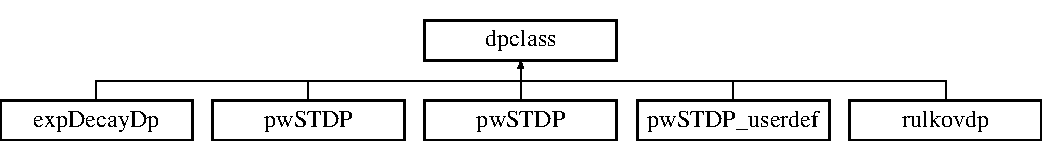
\includegraphics[height=1.898305cm]{db/de6/classdpclass}
\end{center}
\end{figure}
\subsection*{Public Member Functions}
\begin{DoxyCompactItemize}
\item 
\hyperlink{classdpclass_a08441ad6ecfc18420fcc9b715b18ae6c}{dpclass} ()
\item 
virtual float \hyperlink{classdpclass_a4227f736c0ec826d7bda6c98e783d74a}{calculate\+Derived\+Parameter} (int index, vector$<$ float $>$ pars, float dt=1.\+0)
\end{DoxyCompactItemize}


\subsection{Constructor \& Destructor Documentation}
\hypertarget{classdpclass_a08441ad6ecfc18420fcc9b715b18ae6c}{\index{dpclass@{dpclass}!dpclass@{dpclass}}
\index{dpclass@{dpclass}!dpclass@{dpclass}}
\subsubsection[{dpclass}]{\setlength{\rightskip}{0pt plus 5cm}dpclass\+::dpclass (
\begin{DoxyParamCaption}
{}
\end{DoxyParamCaption}
)\hspace{0.3cm}{\ttfamily [inline]}}}\label{classdpclass_a08441ad6ecfc18420fcc9b715b18ae6c}


\subsection{Member Function Documentation}
\hypertarget{classdpclass_a4227f736c0ec826d7bda6c98e783d74a}{\index{dpclass@{dpclass}!calculate\+Derived\+Parameter@{calculate\+Derived\+Parameter}}
\index{calculate\+Derived\+Parameter@{calculate\+Derived\+Parameter}!dpclass@{dpclass}}
\subsubsection[{calculate\+Derived\+Parameter}]{\setlength{\rightskip}{0pt plus 5cm}virtual float dpclass\+::calculate\+Derived\+Parameter (
\begin{DoxyParamCaption}
\item[{int}]{index, }
\item[{vector$<$ float $>$}]{pars, }
\item[{float}]{dt = {\ttfamily 1.0}}
\end{DoxyParamCaption}
)\hspace{0.3cm}{\ttfamily [inline]}, {\ttfamily [virtual]}}}\label{classdpclass_a4227f736c0ec826d7bda6c98e783d74a}


Reimplemented in \hyperlink{classexpDecayDp_adae43a9470a9bf248950fd4bfc31ee04}{exp\+Decay\+Dp}, \hyperlink{classpwSTDP_a29af7a11b93e3617d9da090cc07ad578}{pw\+S\+T\+D\+P}, \hyperlink{classpwSTDP__userdef_ab97adaaca41c96af7bcb70cde27f36cf}{pw\+S\+T\+D\+P\+\_\+userdef}, \hyperlink{classrulkovdp_ac05fee8df961da95972c7343e677660e}{rulkovdp}, and \hyperlink{classpwSTDP_a6c0e3e483e484f8805edd58b7fb37507}{pw\+S\+T\+D\+P}.



The documentation for this class was generated from the following file\+:\begin{DoxyCompactItemize}
\item 
lib/include/\hyperlink{modelSpec_8h}{model\+Spec.\+h}\end{DoxyCompactItemize}

\hypertarget{structerrTupel}{\section{err\+Tupel Struct Reference}
\label{structerrTupel}\index{err\+Tupel@{err\+Tupel}}
}
\subsection*{Public Attributes}
\begin{DoxyCompactItemize}
\item 
unsigned int \hyperlink{structerrTupel_a935755253156aeeda51214ef673690d0}{id}
\item 
double \hyperlink{structerrTupel_a99cafdc91eea024efa6fa2c501d7ff75}{err}
\end{DoxyCompactItemize}


\subsection{Member Data Documentation}
\hypertarget{structerrTupel_a99cafdc91eea024efa6fa2c501d7ff75}{\index{err\+Tupel@{err\+Tupel}!err@{err}}
\index{err@{err}!err\+Tupel@{err\+Tupel}}
\subsubsection[{err}]{\setlength{\rightskip}{0pt plus 5cm}double err\+Tupel\+::err}}\label{structerrTupel_a99cafdc91eea024efa6fa2c501d7ff75}
\hypertarget{structerrTupel_a935755253156aeeda51214ef673690d0}{\index{err\+Tupel@{err\+Tupel}!id@{id}}
\index{id@{id}!err\+Tupel@{err\+Tupel}}
\subsubsection[{id}]{\setlength{\rightskip}{0pt plus 5cm}unsigned int err\+Tupel\+::id}}\label{structerrTupel_a935755253156aeeda51214ef673690d0}


The documentation for this struct was generated from the following file\+:\begin{DoxyCompactItemize}
\item 
userproject/\+H\+H\+Vclamp\+G\+A\+\_\+project/model/\hyperlink{GA_8cc}{G\+A.\+cc}\end{DoxyCompactItemize}

\hypertarget{classexpDecayDp}{\section{exp\+Decay\+Dp Class Reference}
\label{classexpDecayDp}\index{exp\+Decay\+Dp@{exp\+Decay\+Dp}}
}


Class defining the dependent parameter for exponential decay.  




{\ttfamily \#include $<$utils.\+h$>$}

Inheritance diagram for exp\+Decay\+Dp\+:\begin{figure}[H]
\begin{center}
\leavevmode
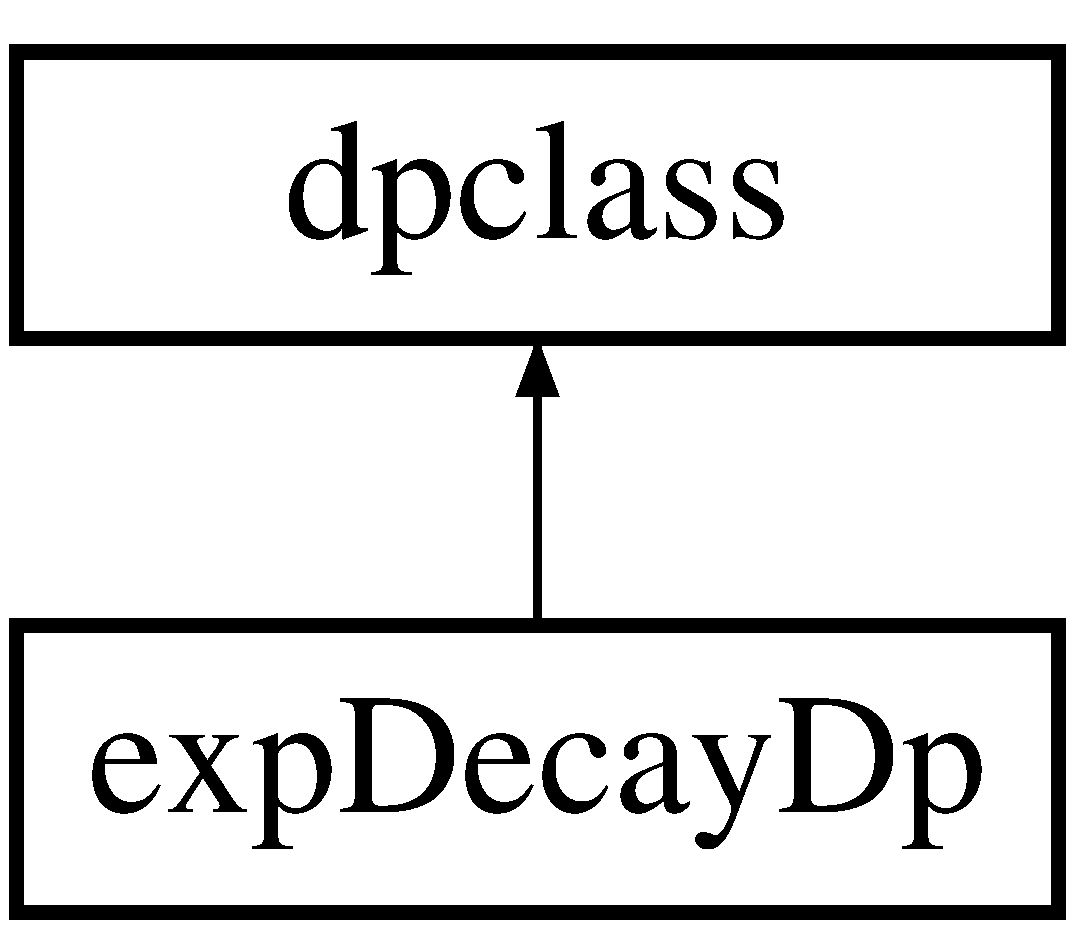
\includegraphics[height=2.000000cm]{da/d0d/classexpDecayDp}
\end{center}
\end{figure}
\subsection*{Public Member Functions}
\begin{DoxyCompactItemize}
\item 
float \hyperlink{classexpDecayDp_adae43a9470a9bf248950fd4bfc31ee04}{calculate\+Derived\+Parameter} (int index, vector$<$ float $>$ pars, float dt=1.\+0)
\item 
float \hyperlink{classexpDecayDp_a6432d17e1ca5e7158970685086a1003e}{exp\+Decay} (vector$<$ float $>$ pars, float dt)
\end{DoxyCompactItemize}


\subsection{Detailed Description}
Class defining the dependent parameter for exponential decay. 

\subsection{Member Function Documentation}
\hypertarget{classexpDecayDp_adae43a9470a9bf248950fd4bfc31ee04}{\index{exp\+Decay\+Dp@{exp\+Decay\+Dp}!calculate\+Derived\+Parameter@{calculate\+Derived\+Parameter}}
\index{calculate\+Derived\+Parameter@{calculate\+Derived\+Parameter}!exp\+Decay\+Dp@{exp\+Decay\+Dp}}
\subsubsection[{calculate\+Derived\+Parameter}]{\setlength{\rightskip}{0pt plus 5cm}float exp\+Decay\+Dp\+::calculate\+Derived\+Parameter (
\begin{DoxyParamCaption}
\item[{int}]{index, }
\item[{vector$<$ float $>$}]{pars, }
\item[{float}]{dt = {\ttfamily 1.0}}
\end{DoxyParamCaption}
)\hspace{0.3cm}{\ttfamily [inline]}, {\ttfamily [virtual]}}}\label{classexpDecayDp_adae43a9470a9bf248950fd4bfc31ee04}


Reimplemented from \hyperlink{classdpclass_a4227f736c0ec826d7bda6c98e783d74a}{dpclass}.

\hypertarget{classexpDecayDp_a6432d17e1ca5e7158970685086a1003e}{\index{exp\+Decay\+Dp@{exp\+Decay\+Dp}!exp\+Decay@{exp\+Decay}}
\index{exp\+Decay@{exp\+Decay}!exp\+Decay\+Dp@{exp\+Decay\+Dp}}
\subsubsection[{exp\+Decay}]{\setlength{\rightskip}{0pt plus 5cm}float exp\+Decay\+Dp\+::exp\+Decay (
\begin{DoxyParamCaption}
\item[{vector$<$ float $>$}]{pars, }
\item[{float}]{dt}
\end{DoxyParamCaption}
)\hspace{0.3cm}{\ttfamily [inline]}}}\label{classexpDecayDp_a6432d17e1ca5e7158970685086a1003e}


The documentation for this class was generated from the following file\+:\begin{DoxyCompactItemize}
\item 
lib/include/\hyperlink{utils_8h}{utils.\+h}\end{DoxyCompactItemize}

\hypertarget{structhistogram}{\section{histogram Struct Reference}
\label{structhistogram}\index{histogram@{histogram}}
}
\subsection*{Public Attributes}
\begin{DoxyCompactItemize}
\item 
unsigned int \hyperlink{structhistogram_a9696f69b741b869f3d569461d527513c}{id}
\item 
unsigned int \hyperlink{structhistogram_a58842f79a6c96378a2bcee46df1664ad}{N}
\end{DoxyCompactItemize}


\subsection{Member Data Documentation}
\hypertarget{structhistogram_a9696f69b741b869f3d569461d527513c}{\index{histogram@{histogram}!id@{id}}
\index{id@{id}!histogram@{histogram}}
\subsubsection[{id}]{\setlength{\rightskip}{0pt plus 5cm}unsigned int histogram\+::id}}\label{structhistogram_a9696f69b741b869f3d569461d527513c}
\hypertarget{structhistogram_a58842f79a6c96378a2bcee46df1664ad}{\index{histogram@{histogram}!N@{N}}
\index{N@{N}!histogram@{histogram}}
\subsubsection[{N}]{\setlength{\rightskip}{0pt plus 5cm}unsigned int histogram\+::\+N}}\label{structhistogram_a58842f79a6c96378a2bcee46df1664ad}


The documentation for this struct was generated from the following file\+:\begin{DoxyCompactItemize}
\item 
userproject/\+M\+Body1\+\_\+project/model/\hyperlink{classol__sim__detailed__output_8cu}{classol\+\_\+sim\+\_\+detailed\+\_\+output.\+cu}\end{DoxyCompactItemize}

\hypertarget{structinputSpec}{\section{input\+Spec Struct Reference}
\label{structinputSpec}\index{input\+Spec@{input\+Spec}}
}


{\ttfamily \#include $<$helper.\+h$>$}

\subsection*{Public Attributes}
\begin{DoxyCompactItemize}
\item 
double \hyperlink{structinputSpec_aa82b84b9475da88190cec34e78478908}{t}
\item 
double \hyperlink{structinputSpec_a6aeb08095e0d0094123108c8a74950a4}{base\+V}
\item 
int \hyperlink{structinputSpec_a25c637510c26633e00ac5f7704dce559}{N}
\item 
vector$<$ double $>$ \hyperlink{structinputSpec_ad88c6e86de04404e7f066b417284414b}{st}
\item 
vector$<$ double $>$ \hyperlink{structinputSpec_a99484aaff897f3d87d4bbfea19f61766}{V}
\end{DoxyCompactItemize}


\subsection{Member Data Documentation}
\hypertarget{structinputSpec_a6aeb08095e0d0094123108c8a74950a4}{\index{input\+Spec@{input\+Spec}!base\+V@{base\+V}}
\index{base\+V@{base\+V}!input\+Spec@{input\+Spec}}
\subsubsection[{base\+V}]{\setlength{\rightskip}{0pt plus 5cm}double input\+Spec\+::base\+V}}\label{structinputSpec_a6aeb08095e0d0094123108c8a74950a4}
\hypertarget{structinputSpec_a25c637510c26633e00ac5f7704dce559}{\index{input\+Spec@{input\+Spec}!N@{N}}
\index{N@{N}!input\+Spec@{input\+Spec}}
\subsubsection[{N}]{\setlength{\rightskip}{0pt plus 5cm}int input\+Spec\+::\+N}}\label{structinputSpec_a25c637510c26633e00ac5f7704dce559}
\hypertarget{structinputSpec_ad88c6e86de04404e7f066b417284414b}{\index{input\+Spec@{input\+Spec}!st@{st}}
\index{st@{st}!input\+Spec@{input\+Spec}}
\subsubsection[{st}]{\setlength{\rightskip}{0pt plus 5cm}vector$<$double$>$ input\+Spec\+::st}}\label{structinputSpec_ad88c6e86de04404e7f066b417284414b}
\hypertarget{structinputSpec_aa82b84b9475da88190cec34e78478908}{\index{input\+Spec@{input\+Spec}!t@{t}}
\index{t@{t}!input\+Spec@{input\+Spec}}
\subsubsection[{t}]{\setlength{\rightskip}{0pt plus 5cm}double input\+Spec\+::t}}\label{structinputSpec_aa82b84b9475da88190cec34e78478908}
\hypertarget{structinputSpec_a99484aaff897f3d87d4bbfea19f61766}{\index{input\+Spec@{input\+Spec}!V@{V}}
\index{V@{V}!input\+Spec@{input\+Spec}}
\subsubsection[{V}]{\setlength{\rightskip}{0pt plus 5cm}vector$<$double$>$ input\+Spec\+::\+V}}\label{structinputSpec_a99484aaff897f3d87d4bbfea19f61766}


The documentation for this struct was generated from the following file\+:\begin{DoxyCompactItemize}
\item 
userproject/\+H\+H\+Vclamp\+G\+A\+\_\+project/model/\hyperlink{helper_8h}{helper.\+h}\end{DoxyCompactItemize}

\hypertarget{structneuronModel}{\section{neuron\+Model Struct Reference}
\label{structneuronModel}\index{neuron\+Model@{neuron\+Model}}
}


class (struct) for specifying a neuron model.  




{\ttfamily \#include $<$model\+Spec.\+h$>$}

\subsection*{Public Attributes}
\begin{DoxyCompactItemize}
\item 
string \hyperlink{structneuronModel_a9e6536fd15b69fa24b708e41f97df899}{sim\+Code}
\begin{DoxyCompactList}\small\item\em Code that defines the execution of one timestep of integration of the neuron model. \end{DoxyCompactList}\item 
string \hyperlink{structneuronModel_a9b0fae36963fb760040c3b1d22bee25c}{threshold\+Condition\+Code}
\begin{DoxyCompactList}\small\item\em Code evaluating to a bool (e.\+g. \char`\"{}\+V $>$ 20\char`\"{}) that defines the condition for a true spike in the described neuron model. \end{DoxyCompactList}\item 
string \hyperlink{structneuronModel_ad97df9af00fba946865debf6cd539217}{reset\+Code}
\begin{DoxyCompactList}\small\item\em Code that defines the reset action taken after a spike occurred. This can be empty. \end{DoxyCompactList}\item 
vector$<$ string $>$ \hyperlink{structneuronModel_a9a9156ffb643572fd67f6e585ef79ad0}{var\+Names}
\begin{DoxyCompactList}\small\item\em Names of the variables in the neuron model. \end{DoxyCompactList}\item 
vector$<$ string $>$ \hyperlink{structneuronModel_ab193cb434db2df5f1fa9a79fba30af83}{tmp\+Var\+Names}
\begin{DoxyCompactList}\small\item\em never used \end{DoxyCompactList}\item 
vector$<$ string $>$ \hyperlink{structneuronModel_a86788cb29131da0a26ce79693a076352}{var\+Types}
\begin{DoxyCompactList}\small\item\em Types of the variable named above, e.\+g. \char`\"{}float\char`\"{}. Names and types are matched by their order of occurrence in the vector. \end{DoxyCompactList}\item 
vector$<$ string $>$ \hyperlink{structneuronModel_a3f5668e85624014cd5de97bf00d2b82f}{tmp\+Var\+Types}
\begin{DoxyCompactList}\small\item\em never used \end{DoxyCompactList}\item 
vector$<$ string $>$ \hyperlink{structneuronModel_a4a5bf1f757a72b6edc28ad26ed61b2be}{p\+Names}
\begin{DoxyCompactList}\small\item\em Names of (independent) parameters of the model. These are assumed to be always of type \char`\"{}float\char`\"{}. \end{DoxyCompactList}\item 
vector$<$ string $>$ \hyperlink{structneuronModel_a051c0c704ce383c43cdf446accbeb201}{dp\+Names}
\begin{DoxyCompactList}\small\item\em Names of dependent parameters of the model. These are assumed to be always of type \char`\"{}float\char`\"{}. \end{DoxyCompactList}\item 
vector$<$ string $>$ \hyperlink{structneuronModel_a00094db5e89eaa5d8017d83d84c63676}{extra\+Global\+Neuron\+Kernel\+Parameters}
\begin{DoxyCompactList}\small\item\em Additional parameter in the neuron kernel; it is translated to a population specific name but otherwise assumed to be one parameter per population rather than per neuron. \end{DoxyCompactList}\item 
vector$<$ string $>$ \hyperlink{structneuronModel_a35592a2fad7d926ca664871bd1513f24}{extra\+Global\+Neuron\+Kernel\+Parameter\+Types}
\begin{DoxyCompactList}\small\item\em Additional parameters in the neuron kernel; they are translated to a population specific name but otherwise assumed to be one parameter per population rather than per neuron. \end{DoxyCompactList}\item 
\hyperlink{classdpclass}{dpclass} $\ast$ \hyperlink{structneuronModel_a9b9b9e5e66702eb114b268bbd08d7c34}{dps}
\item 
bool \hyperlink{structneuronModel_aff3d8b2160410c976506e0c4ddf8b6c1}{need\+Pre\+St}
\item 
bool \hyperlink{structneuronModel_a633acff33b8b640f7a815f357b144117}{need\+Post\+St}
\end{DoxyCompactItemize}


\subsection{Detailed Description}
class (struct) for specifying a neuron model. 

\subsection{Member Data Documentation}
\hypertarget{structneuronModel_a051c0c704ce383c43cdf446accbeb201}{\index{neuron\+Model@{neuron\+Model}!dp\+Names@{dp\+Names}}
\index{dp\+Names@{dp\+Names}!neuron\+Model@{neuron\+Model}}
\subsubsection[{dp\+Names}]{\setlength{\rightskip}{0pt plus 5cm}vector$<$string$>$ neuron\+Model\+::dp\+Names}}\label{structneuronModel_a051c0c704ce383c43cdf446accbeb201}


Names of dependent parameters of the model. These are assumed to be always of type \char`\"{}float\char`\"{}. 

The dependent parameters are functions of independent parameters that enter into the neuron model. To avoid unecessary computational overhead, these parameters are calculated at compile time and inserted as explicit values into the generated code. See method N\+Nmodel\+::init\+Derived\+Neuron\+Para for how this is done. \hypertarget{structneuronModel_a9b9b9e5e66702eb114b268bbd08d7c34}{\index{neuron\+Model@{neuron\+Model}!dps@{dps}}
\index{dps@{dps}!neuron\+Model@{neuron\+Model}}
\subsubsection[{dps}]{\setlength{\rightskip}{0pt plus 5cm}{\bf dpclass}$\ast$ neuron\+Model\+::dps}}\label{structneuronModel_a9b9b9e5e66702eb114b268bbd08d7c34}
\hypertarget{structneuronModel_a00094db5e89eaa5d8017d83d84c63676}{\index{neuron\+Model@{neuron\+Model}!extra\+Global\+Neuron\+Kernel\+Parameters@{extra\+Global\+Neuron\+Kernel\+Parameters}}
\index{extra\+Global\+Neuron\+Kernel\+Parameters@{extra\+Global\+Neuron\+Kernel\+Parameters}!neuron\+Model@{neuron\+Model}}
\subsubsection[{extra\+Global\+Neuron\+Kernel\+Parameters}]{\setlength{\rightskip}{0pt plus 5cm}vector$<$string$>$ neuron\+Model\+::extra\+Global\+Neuron\+Kernel\+Parameters}}\label{structneuronModel_a00094db5e89eaa5d8017d83d84c63676}


Additional parameter in the neuron kernel; it is translated to a population specific name but otherwise assumed to be one parameter per population rather than per neuron. 

\hypertarget{structneuronModel_a35592a2fad7d926ca664871bd1513f24}{\index{neuron\+Model@{neuron\+Model}!extra\+Global\+Neuron\+Kernel\+Parameter\+Types@{extra\+Global\+Neuron\+Kernel\+Parameter\+Types}}
\index{extra\+Global\+Neuron\+Kernel\+Parameter\+Types@{extra\+Global\+Neuron\+Kernel\+Parameter\+Types}!neuron\+Model@{neuron\+Model}}
\subsubsection[{extra\+Global\+Neuron\+Kernel\+Parameter\+Types}]{\setlength{\rightskip}{0pt plus 5cm}vector$<$string$>$ neuron\+Model\+::extra\+Global\+Neuron\+Kernel\+Parameter\+Types}}\label{structneuronModel_a35592a2fad7d926ca664871bd1513f24}


Additional parameters in the neuron kernel; they are translated to a population specific name but otherwise assumed to be one parameter per population rather than per neuron. 

\hypertarget{structneuronModel_a633acff33b8b640f7a815f357b144117}{\index{neuron\+Model@{neuron\+Model}!need\+Post\+St@{need\+Post\+St}}
\index{need\+Post\+St@{need\+Post\+St}!neuron\+Model@{neuron\+Model}}
\subsubsection[{need\+Post\+St}]{\setlength{\rightskip}{0pt plus 5cm}bool neuron\+Model\+::need\+Post\+St}}\label{structneuronModel_a633acff33b8b640f7a815f357b144117}
\hypertarget{structneuronModel_aff3d8b2160410c976506e0c4ddf8b6c1}{\index{neuron\+Model@{neuron\+Model}!need\+Pre\+St@{need\+Pre\+St}}
\index{need\+Pre\+St@{need\+Pre\+St}!neuron\+Model@{neuron\+Model}}
\subsubsection[{need\+Pre\+St}]{\setlength{\rightskip}{0pt plus 5cm}bool neuron\+Model\+::need\+Pre\+St}}\label{structneuronModel_aff3d8b2160410c976506e0c4ddf8b6c1}
\hypertarget{structneuronModel_a4a5bf1f757a72b6edc28ad26ed61b2be}{\index{neuron\+Model@{neuron\+Model}!p\+Names@{p\+Names}}
\index{p\+Names@{p\+Names}!neuron\+Model@{neuron\+Model}}
\subsubsection[{p\+Names}]{\setlength{\rightskip}{0pt plus 5cm}vector$<$string$>$ neuron\+Model\+::p\+Names}}\label{structneuronModel_a4a5bf1f757a72b6edc28ad26ed61b2be}


Names of (independent) parameters of the model. These are assumed to be always of type \char`\"{}float\char`\"{}. 

\hypertarget{structneuronModel_ad97df9af00fba946865debf6cd539217}{\index{neuron\+Model@{neuron\+Model}!reset\+Code@{reset\+Code}}
\index{reset\+Code@{reset\+Code}!neuron\+Model@{neuron\+Model}}
\subsubsection[{reset\+Code}]{\setlength{\rightskip}{0pt plus 5cm}string neuron\+Model\+::reset\+Code}}\label{structneuronModel_ad97df9af00fba946865debf6cd539217}


Code that defines the reset action taken after a spike occurred. This can be empty. 

\hypertarget{structneuronModel_a9e6536fd15b69fa24b708e41f97df899}{\index{neuron\+Model@{neuron\+Model}!sim\+Code@{sim\+Code}}
\index{sim\+Code@{sim\+Code}!neuron\+Model@{neuron\+Model}}
\subsubsection[{sim\+Code}]{\setlength{\rightskip}{0pt plus 5cm}string neuron\+Model\+::sim\+Code}}\label{structneuronModel_a9e6536fd15b69fa24b708e41f97df899}


Code that defines the execution of one timestep of integration of the neuron model. 

The code will refer to  for the value of the variable with name \char`\"{}\+N\+N\char`\"{}. It needs to refer to the predefined variable \char`\"{}\+I\+S\+Y\+N\char`\"{}, i.\+e. contain , if it is to receive input. \hypertarget{structneuronModel_a9b0fae36963fb760040c3b1d22bee25c}{\index{neuron\+Model@{neuron\+Model}!threshold\+Condition\+Code@{threshold\+Condition\+Code}}
\index{threshold\+Condition\+Code@{threshold\+Condition\+Code}!neuron\+Model@{neuron\+Model}}
\subsubsection[{threshold\+Condition\+Code}]{\setlength{\rightskip}{0pt plus 5cm}string neuron\+Model\+::threshold\+Condition\+Code}}\label{structneuronModel_a9b0fae36963fb760040c3b1d22bee25c}


Code evaluating to a bool (e.\+g. \char`\"{}\+V $>$ 20\char`\"{}) that defines the condition for a true spike in the described neuron model. 

\hypertarget{structneuronModel_ab193cb434db2df5f1fa9a79fba30af83}{\index{neuron\+Model@{neuron\+Model}!tmp\+Var\+Names@{tmp\+Var\+Names}}
\index{tmp\+Var\+Names@{tmp\+Var\+Names}!neuron\+Model@{neuron\+Model}}
\subsubsection[{tmp\+Var\+Names}]{\setlength{\rightskip}{0pt plus 5cm}vector$<$string$>$ neuron\+Model\+::tmp\+Var\+Names}}\label{structneuronModel_ab193cb434db2df5f1fa9a79fba30af83}


never used 

\hypertarget{structneuronModel_a3f5668e85624014cd5de97bf00d2b82f}{\index{neuron\+Model@{neuron\+Model}!tmp\+Var\+Types@{tmp\+Var\+Types}}
\index{tmp\+Var\+Types@{tmp\+Var\+Types}!neuron\+Model@{neuron\+Model}}
\subsubsection[{tmp\+Var\+Types}]{\setlength{\rightskip}{0pt plus 5cm}vector$<$string$>$ neuron\+Model\+::tmp\+Var\+Types}}\label{structneuronModel_a3f5668e85624014cd5de97bf00d2b82f}


never used 

\hypertarget{structneuronModel_a9a9156ffb643572fd67f6e585ef79ad0}{\index{neuron\+Model@{neuron\+Model}!var\+Names@{var\+Names}}
\index{var\+Names@{var\+Names}!neuron\+Model@{neuron\+Model}}
\subsubsection[{var\+Names}]{\setlength{\rightskip}{0pt plus 5cm}vector$<$string$>$ neuron\+Model\+::var\+Names}}\label{structneuronModel_a9a9156ffb643572fd67f6e585ef79ad0}


Names of the variables in the neuron model. 

\hypertarget{structneuronModel_a86788cb29131da0a26ce79693a076352}{\index{neuron\+Model@{neuron\+Model}!var\+Types@{var\+Types}}
\index{var\+Types@{var\+Types}!neuron\+Model@{neuron\+Model}}
\subsubsection[{var\+Types}]{\setlength{\rightskip}{0pt plus 5cm}vector$<$string$>$ neuron\+Model\+::var\+Types}}\label{structneuronModel_a86788cb29131da0a26ce79693a076352}


Types of the variable named above, e.\+g. \char`\"{}float\char`\"{}. Names and types are matched by their order of occurrence in the vector. 



The documentation for this struct was generated from the following file\+:\begin{DoxyCompactItemize}
\item 
lib/include/\hyperlink{modelSpec_8h}{model\+Spec.\+h}\end{DoxyCompactItemize}

\hypertarget{classNNmodel}{\section{N\+Nmodel Class Reference}
\label{classNNmodel}\index{N\+Nmodel@{N\+Nmodel}}
}


Structure to hold the information that defines synapse dynamics (a model of how synapse variables change over time, independent of or in addition to changes when spikes occur).  




{\ttfamily \#include $<$model\+Spec.\+h$>$}

\subsection*{Public Member Functions}
\begin{DoxyCompactItemize}
\item 
\hyperlink{classNNmodel_a91216d74536a5871c507af7f40cd2d64}{N\+Nmodel} ()
\item 
\hyperlink{classNNmodel_aa9f519391df5f08c4ec5f59578ac5ffc}{$\sim$\+N\+Nmodel} ()
\item 
void \hyperlink{classNNmodel_a757eff2a5877688e6e5492726df035ee}{set\+Name} (const string)
\begin{DoxyCompactList}\small\item\em Method to set the neuronal network model name. \end{DoxyCompactList}\item 
void \hyperlink{classNNmodel_a44fb38b93216c56254fbbee6175cffd1}{set\+Precision} (unsigned int)
\begin{DoxyCompactList}\small\item\em Set numerical precision for floating point. \end{DoxyCompactList}\item 
void \hyperlink{classNNmodel_ab843183abd01171e9a8ab99b219cb2b7}{set\+Timing} (bool)
\begin{DoxyCompactList}\small\item\em Set whether timers and timing commands are to be included. \end{DoxyCompactList}\item 
void \hyperlink{classNNmodel_acc6b868fe6383bbea589ba2eddfac679}{set\+Seed} (unsigned int)
\begin{DoxyCompactList}\small\item\em Set the random seed (disables automatic seeding if argument not 0). \end{DoxyCompactList}\item 
void \hyperlink{classNNmodel_aa096950a3bb9a7d573df77c26919ab07}{check\+Sizes} (unsigned int $\ast$, unsigned int $\ast$, unsigned int $\ast$)
\item 
void \hyperlink{classNNmodel_a836c19f5ebf90740b18f6291b0c03732}{reset\+Padded\+Sums} ()
\begin{DoxyCompactList}\small\item\em Re-\/calculates the block-\/size-\/padded sum of threads needed to compute the groups of neurons and synapses assigned to each device. Must be called after changing the host\+I\+D\+:device\+I\+D of any group. \end{DoxyCompactList}\item 
void \hyperlink{classNNmodel_ae44b078dcca0b16ef45978a7fe54d16e}{set\+G\+P\+U\+Device} (int)
\begin{DoxyCompactList}\small\item\em Method to choose the G\+P\+U to be used for the model. If "A\+U\+T\+O\+D\+E\+V\+I\+C\+E' (-\/1), Ge\+N\+N will choose the device based on a heuristic rule. \end{DoxyCompactList}\item 
void \hyperlink{classNNmodel_a24532739d3ae98da3e00a9fe5aadd54e}{add\+Neuron\+Population} (const char $\ast$, unsigned int, unsigned int, float $\ast$, float $\ast$)
\begin{DoxyCompactList}\small\item\em Method for adding a neuron population to a neuronal network model, using C style character array for the name of the population. \end{DoxyCompactList}\item 
void \hyperlink{classNNmodel_af52eebfac8ff3cd3eaa4f2cfc0918e3a}{add\+Neuron\+Population} (const string, unsigned int, unsigned int, float $\ast$, float $\ast$)
\begin{DoxyCompactList}\small\item\em Method for adding a neuron population to a neuronal network model, using C++ string for the name of the population. \end{DoxyCompactList}\item 
void \hyperlink{classNNmodel_a95724e1798bd9ac5642a8fb2484a2f93}{activate\+Direct\+Input} (const string, unsigned int)
\begin{DoxyCompactList}\small\item\em This function defines the type of the explicit input to the neuron model. Current options are common constant input to all neurons, input from a file and input defines as a rule. \end{DoxyCompactList}\item 
void \hyperlink{classNNmodel_a9630c120beba41655f1f23e6dd21242e}{set\+Const\+Inp} (const string, float)
\begin{DoxyCompactList}\small\item\em Method for setting the global input value for a neuron population if C\+O\+N\+S\+T\+I\+N\+P. \end{DoxyCompactList}\item 
void \hyperlink{classNNmodel_a65aee794c66069cd3e6316ade0c91192}{set\+Neuron\+Cluster\+Index} (const string neuron\+Group, int host\+I\+D, int device\+I\+D)
\begin{DoxyCompactList}\small\item\em Function for setting which host and which device a neuron group will be simulated on. \end{DoxyCompactList}\item 
void \hyperlink{classNNmodel_a9dceb36a7d36c82adfdb5642df8f25f7}{add\+Synapse\+Population} (const string \hyperlink{classNNmodel_a7d81556b7b15a4a625b23f965944dae9}{name}, unsigned int syntype, unsigned int conntype, unsigned int gtype, const string src, const string trg, float $\ast$p)
\begin{DoxyCompactList}\small\item\em Overload of method for backwards compatibility. \end{DoxyCompactList}\item 
void \hyperlink{classNNmodel_ac82f4463de85aa6e345bc52518eb1f75}{add\+Synapse\+Population} (const char $\ast$, unsigned int, unsigned int, unsigned int, unsigned int, unsigned int, const char $\ast$, const char $\ast$, float $\ast$, float $\ast$, float $\ast$)
\begin{DoxyCompactList}\small\item\em Method for adding a synapse population to a neuronal network model, using C style character array for the name of the population. \end{DoxyCompactList}\item 
void \hyperlink{classNNmodel_aa31885e04282660f34e452c1310ef20e}{add\+Synapse\+Population} (const string, unsigned int, unsigned int, unsigned int, unsigned int, unsigned int, const string, const string, float $\ast$, float $\ast$, float $\ast$)
\begin{DoxyCompactList}\small\item\em Overloaded version without initial variables for synapses. \end{DoxyCompactList}\item 
void \hyperlink{classNNmodel_ac84ccb2f8e4dc3e3343fb663adedc460}{add\+Synapse\+Population} (const string, unsigned int, unsigned int, unsigned int, unsigned int, unsigned int, const string, const string, float $\ast$, float $\ast$, float $\ast$, float $\ast$)
\begin{DoxyCompactList}\small\item\em Method for adding a synapse population to a neuronal network model, using C++ string for the name of the population. \end{DoxyCompactList}\item 
void \hyperlink{classNNmodel_a06dd91d3a28b70b444e0866859a348f7}{set\+Synapse\+G} (const string, float)
\begin{DoxyCompactList}\small\item\em Method for setting the conductance (g) value for a synapse population with \char`\"{}\+G\+L\+O\+B\+A\+L\+G\char`\"{} charactertistic. \end{DoxyCompactList}\item 
void \hyperlink{classNNmodel_abcd74b0eb3c2696069320bd929070d4b}{set\+Max\+Conn} (const string, unsigned int)
\begin{DoxyCompactList}\small\item\em This function defines the maximum number of connections for a neuron in the population. \end{DoxyCompactList}\item 
void \hyperlink{classNNmodel_a2b7ad279fd8e68d951957f21bbb072c5}{set\+Synapse\+Cluster\+Index} (const string synapse\+Group, int host\+I\+D, int device\+I\+D)
\begin{DoxyCompactList}\small\item\em Function for setting which host and which device a synapse group will be simulated on. \end{DoxyCompactList}\item 
void \hyperlink{classNNmodel_a3de3cfc04cb28e939225341ee10e2119}{init\+Learn\+Grps} ()
\end{DoxyCompactItemize}
\subsection*{Public Attributes}
\begin{DoxyCompactItemize}
\item 
string \hyperlink{classNNmodel_a7d81556b7b15a4a625b23f965944dae9}{name}
\begin{DoxyCompactList}\small\item\em Name of the neuronal newtwork model. \end{DoxyCompactList}\item 
string \hyperlink{classNNmodel_a917241001f3469a569dbb91aaa6a4039}{ftype}
\begin{DoxyCompactList}\small\item\em Type of floating point variables (float, double, ...; default\+: float) \end{DoxyCompactList}\item 
string \hyperlink{classNNmodel_ae02892a44b18e3ce913dc43dc31dd380}{R\+Ntype}
\begin{DoxyCompactList}\small\item\em Underlying type for random number generation (default\+: long) \end{DoxyCompactList}\item 
int \hyperlink{classNNmodel_ad09a7a4c3888876f7a95e8d5e344c71e}{valid}
\begin{DoxyCompactList}\small\item\em Flag for whether the model has been validated (unused?) \end{DoxyCompactList}\item 
unsigned int \hyperlink{classNNmodel_ab5f42229881455bed0f484b6d0211795}{need\+St}
\begin{DoxyCompactList}\small\item\em Whether last spike times are needed at all in this network model (related to S\+T\+D\+P) \end{DoxyCompactList}\item 
unsigned int \hyperlink{classNNmodel_aa6753d648bcac06109f0820349b5d2be}{need\+Synapse\+Delay}
\begin{DoxyCompactList}\small\item\em Whether delayed synapse conductance is required in the network. \end{DoxyCompactList}\item 
int \hyperlink{classNNmodel_a79631e0c13cdd5ebed55a16bea15819a}{choose\+G\+P\+U\+Device}
\item 
bool \hyperlink{classNNmodel_afae2a91984509205ff07afc948cbf106}{timing}
\item 
unsigned int \hyperlink{classNNmodel_ad82f4dbcf4cc6a942965f9ecaa79616a}{seed}
\item 
bool \hyperlink{classNNmodel_a17091f9688dbfa4e9f2d83181a1b554a}{need\+Spk\+Evnt}
\item 
vector$<$ string $>$ \hyperlink{classNNmodel_af3c7ec6917040e62be5cee3505c330a8}{neuron\+Name}
\begin{DoxyCompactList}\small\item\em Names of neuron groups. \end{DoxyCompactList}\item 
unsigned int \hyperlink{classNNmodel_a383562e3f02192f58a6150a4ca0861c5}{neuron\+Grp\+N}
\begin{DoxyCompactList}\small\item\em Number of neuron groups. \end{DoxyCompactList}\item 
vector$<$ unsigned int $>$ \hyperlink{classNNmodel_a87d3de14d0d5c7183199fea48c04b949}{neuron\+N}
\begin{DoxyCompactList}\small\item\em Number of neurons in group. \end{DoxyCompactList}\item 
vector$<$ unsigned int $>$ \hyperlink{classNNmodel_a84cf2761cf76d70a06f871a77e64c0b4}{sum\+Neuron\+N}
\begin{DoxyCompactList}\small\item\em Summed neuron numbers. \end{DoxyCompactList}\item 
vector$<$ unsigned int $>$ \hyperlink{classNNmodel_a08d284601fc39e164ca5aeac399d6a59}{pad\+Sum\+Neuron\+N}
\begin{DoxyCompactList}\small\item\em Padded summed neuron numbers. \end{DoxyCompactList}\item 
vector$<$ unsigned int $>$ \hyperlink{classNNmodel_aec217846b4a0eeb38bfec1209319dd81}{neuron\+Post\+Syn}
\item 
vector$<$ unsigned int $>$ \hyperlink{classNNmodel_a0e5087ec30e3efb114f8f713759a4abc}{neuron\+Type}
\begin{DoxyCompactList}\small\item\em Postsynaptic methods to the neuron. \end{DoxyCompactList}\item 
vector$<$ vector$<$ float $>$ $>$ \hyperlink{classNNmodel_a4711c16ac1dc4bd09255f69a3469a4bd}{neuron\+Para}
\begin{DoxyCompactList}\small\item\em Parameters of neurons. \end{DoxyCompactList}\item 
vector$<$ vector$<$ float $>$ $>$ \hyperlink{classNNmodel_a7f834f3863c06a5b2381c0adddb901b8}{dnp}
\begin{DoxyCompactList}\small\item\em Derived neuron parameters. \end{DoxyCompactList}\item 
vector$<$ vector$<$ float $>$ $>$ \hyperlink{classNNmodel_a04c2e61ef297c1e0fd3f0acb32f79a17}{neuron\+Ini}
\begin{DoxyCompactList}\small\item\em Initial values of neurons. \end{DoxyCompactList}\item 
vector$<$ vector$<$ unsigned int $>$ $>$ \hyperlink{classNNmodel_af3f5459e9438989b12e4b675352dd258}{in\+Syn}
\begin{DoxyCompactList}\small\item\em The ids of the incoming synapse groups. \end{DoxyCompactList}\item 
vector$<$ vector$<$ unsigned int $>$ $>$ \hyperlink{classNNmodel_a6ba57b83448ab23eaa5a68d40b2ceac9}{out\+Syn}
\begin{DoxyCompactList}\small\item\em The ids of the outgoing synapse groups. \end{DoxyCompactList}\item 
vector$<$ unsigned int $>$ \hyperlink{classNNmodel_acd0592315c59ac3c0e0dbe9bb35d7004}{receives\+Input\+Current}
\begin{DoxyCompactList}\small\item\em flags whether neurons of a population receive explicit input currents \end{DoxyCompactList}\item 
vector$<$ bool $>$ \hyperlink{classNNmodel_ad14509938bfeb7f2fc8f011d2ec995ac}{neuron\+Need\+St}
\begin{DoxyCompactList}\small\item\em Whether last spike time needs to be saved for each indivual neuron type. \end{DoxyCompactList}\item 
vector$<$ bool $>$ \hyperlink{classNNmodel_abd22d449a48437fbf4e090b553f471f8}{neuron\+Need\+Spk\+Evnt}
\begin{DoxyCompactList}\small\item\em Whether this neuron group needs to record spike like events. \end{DoxyCompactList}\item 
vector$<$ string $>$ \hyperlink{classNNmodel_a2107fc30756637a876374ad35d69a19b}{neuron\+Spk\+Evnt\+Condition}
\begin{DoxyCompactList}\small\item\em Will contain the spike event condition code when spike events are used. \end{DoxyCompactList}\item 
vector$<$ unsigned int $>$ \hyperlink{classNNmodel_a0801942c5e41585da01b2c341f1e9f55}{neuron\+Delay\+Slots}
\begin{DoxyCompactList}\small\item\em The number of slots needed in the synapse delay queues of a neuron group. \end{DoxyCompactList}\item 
vector$<$ int $>$ \hyperlink{classNNmodel_a1ddf63324795faf42f32e4cf4a82a0e2}{neuron\+Host\+I\+D}
\begin{DoxyCompactList}\small\item\em The I\+D of the cluster node which the neuron groups are computed on. \end{DoxyCompactList}\item 
vector$<$ int $>$ \hyperlink{classNNmodel_a67ec0b349b4f423712b7636a3cc2fa1e}{neuron\+Device\+I\+D}
\begin{DoxyCompactList}\small\item\em The I\+D of the C\+U\+D\+A device which the neuron groups are comnputed on. \end{DoxyCompactList}\item 
vector$<$ vector$<$ bool $>$ $>$ \hyperlink{classNNmodel_a6cd30ae92d9eef399beb66098d016774}{neuron\+Var\+Need\+Spk\+Evnt}
\begin{DoxyCompactList}\small\item\em indicates whether spk\+Ent values (or delay queues) need to be stored for this variable \end{DoxyCompactList}\item 
vector$<$ vector$<$ bool $>$ $>$ \hyperlink{classNNmodel_a69a2c9a2317316d0eddf4033779f17cc}{neuron\+Var\+Need\+Spk}
\begin{DoxyCompactList}\small\item\em indicates whether spk values (or delay queues) need to be stored for this variable \end{DoxyCompactList}\item 
vector$<$ string $>$ \hyperlink{classNNmodel_a13993564faeb0e67a21b3c9ffababaf1}{synapse\+Name}
\begin{DoxyCompactList}\small\item\em Names of synapse groups. \end{DoxyCompactList}\item 
unsigned int \hyperlink{classNNmodel_a1e6209fc2014ab9f1820a614cc246c67}{synapse\+Grp\+N}
\begin{DoxyCompactList}\small\item\em Number of synapse groups. \end{DoxyCompactList}\item 
vector$<$ unsigned int $>$ \hyperlink{classNNmodel_a03e34fda1008acf6379f80e8d713d41b}{sum\+Synapse\+Trg\+N}
\begin{DoxyCompactList}\small\item\em Summed number of target neurons. \end{DoxyCompactList}\item 
vector$<$ unsigned int $>$ \hyperlink{classNNmodel_a73881a9d190c544cc6add9a19ee6a304}{pad\+Sum\+Synapse\+Trg\+N}
\begin{DoxyCompactList}\small\item\em \char`\"{}\+Padded\char`\"{} summed target neuron numbers \end{DoxyCompactList}\item 
vector$<$ unsigned int $>$ \hyperlink{classNNmodel_afd62bf5791467b37ef06b025ae419d36}{max\+Conn}
\begin{DoxyCompactList}\small\item\em Padded summed maximum number of connections for a neuron in the neuron groups. \end{DoxyCompactList}\item 
vector$<$ unsigned int $>$ \hyperlink{classNNmodel_a7c0e09e6fe2327601cc9b1e2e995b0e9}{pad\+Sum\+Synapse\+Krnl}
\item 
vector$<$ unsigned int $>$ \hyperlink{classNNmodel_a5945dd8a2936f38a5997a5cae51cf706}{synapse\+Type}
\begin{DoxyCompactList}\small\item\em Types of synapses. \end{DoxyCompactList}\item 
vector$<$ unsigned int $>$ \hyperlink{classNNmodel_a0b1d2c6f24b8ed9215dce9daf3ca0518}{synapse\+Conn\+Type}
\begin{DoxyCompactList}\small\item\em Connectivity type of synapses. \end{DoxyCompactList}\item 
vector$<$ unsigned int $>$ \hyperlink{classNNmodel_a521aa25f9cc763dab52769da0b775470}{synapse\+G\+Type}
\begin{DoxyCompactList}\small\item\em Type of specification method for synaptic conductance. \end{DoxyCompactList}\item 
vector$<$ unsigned int $>$ \hyperlink{classNNmodel_a39861eefc8f7b13c21aaf82142520227}{synapse\+Source}
\begin{DoxyCompactList}\small\item\em Presynaptic neuron groups. \end{DoxyCompactList}\item 
vector$<$ unsigned int $>$ \hyperlink{classNNmodel_a10c4e0a9d71bbfa6895de30a64f31ca6}{synapse\+Target}
\begin{DoxyCompactList}\small\item\em Postsynaptic neuron groups. \end{DoxyCompactList}\item 
vector$<$ unsigned int $>$ \hyperlink{classNNmodel_adc8ccfb003c34fbca10d0fd0e3b26ee0}{synapse\+In\+Syn\+No}
\begin{DoxyCompactList}\small\item\em I\+Ds of the target neurons' incoming synapse variables for each synapse group. \end{DoxyCompactList}\item 
vector$<$ unsigned int $>$ \hyperlink{classNNmodel_a7d6d9860957c931725cead04ee0d6d98}{synapse\+Out\+Syn\+No}
\begin{DoxyCompactList}\small\item\em The target neurons' outgoing synapse for each synapse group. \end{DoxyCompactList}\item 
vector$<$ unsigned int $>$ \hyperlink{classNNmodel_a5d70d70919f892c66196fdea7cb13a45}{uses\+True\+Spikes}
\begin{DoxyCompactList}\small\item\em Defines if synapse update is done after detection of real spikes (only one point after threshold) \end{DoxyCompactList}\item 
vector$<$ unsigned int $>$ \hyperlink{classNNmodel_a5d1a849b688fd0b7fdb999d39b5e049b}{uses\+Spike\+Events}
\begin{DoxyCompactList}\small\item\em Defines if synapse update is done after detection of spike events (every point above threshold) \end{DoxyCompactList}\item 
vector$<$ vector$<$ string $>$ $>$ \hyperlink{classNNmodel_a30e4ebc1109de5e7d921b22f1597cbf4}{synapse\+Spk\+Evnt\+Vars}
\begin{DoxyCompactList}\small\item\em Defines variable names that are needed in the Spk\+Evnt condition and that are pre-\/fetched for that purpose into shared memory. \end{DoxyCompactList}\item 
vector$<$ unsigned int $>$ \hyperlink{classNNmodel_a81fb25a9fab59e840ef622d469747d69}{uses\+Post\+Learning}
\begin{DoxyCompactList}\small\item\em Defines if anything is done in case of postsynaptic neuron spiking before presynaptic neuron (punishment in S\+T\+D\+P etc.) \end{DoxyCompactList}\item 
vector$<$ vector$<$ float $>$ $>$ \hyperlink{classNNmodel_a65795cabef5f0d1f75e8c08530750d0e}{synapse\+Para}
\begin{DoxyCompactList}\small\item\em parameters of synapses \end{DoxyCompactList}\item 
vector$<$ vector$<$ float $>$ $>$ \hyperlink{classNNmodel_a0b82703b2b3726e86116767f2bc0c422}{synapse\+Ini}
\begin{DoxyCompactList}\small\item\em Initial values of synapse variables. \end{DoxyCompactList}\item 
vector$<$ vector$<$ float $>$ $>$ \hyperlink{classNNmodel_aeb5fa229c8032952feb3440e055f6a85}{dsp\+\_\+w}
\begin{DoxyCompactList}\small\item\em Derived synapse parameters (\hyperlink{classweightUpdateModel}{weight\+Update\+Model} only) \end{DoxyCompactList}\item 
vector$<$ unsigned int $>$ \hyperlink{classNNmodel_a4fc23591415ddac76d1d92ab68c018c9}{post\+Synapse\+Type}
\begin{DoxyCompactList}\small\item\em Types of post-\/synaptic model. \end{DoxyCompactList}\item 
vector$<$ vector$<$ float $>$ $>$ \hyperlink{classNNmodel_a3b9431104ee496ed084ab549ebf2de10}{post\+Synapse\+Para}
\begin{DoxyCompactList}\small\item\em parameters of postsynapses \end{DoxyCompactList}\item 
vector$<$ vector$<$ float $>$ $>$ \hyperlink{classNNmodel_a82827284185d5c39e4e04e14cf612253}{post\+Syn\+Ini}
\begin{DoxyCompactList}\small\item\em Initial values of postsynaptic variables. \end{DoxyCompactList}\item 
vector$<$ vector$<$ float $>$ $>$ \hyperlink{classNNmodel_aa03452826c44c9af81eba7a618de7e09}{dpsp}
\begin{DoxyCompactList}\small\item\em Derived postsynapse parameters. \end{DoxyCompactList}\item 
vector$<$ float $>$ \hyperlink{classNNmodel_a8df5fd36faa5a56edea7d287fea1f625}{global\+Inp}
\begin{DoxyCompactList}\small\item\em Global explicit input if C\+O\+N\+S\+T\+I\+N\+P is chosen. \end{DoxyCompactList}\item 
unsigned int \hyperlink{classNNmodel_aa0e25f384103db3bcc8c8b0425ae01b3}{lrn\+Groups}
\begin{DoxyCompactList}\small\item\em Number of synapse groups with learning. \end{DoxyCompactList}\item 
vector$<$ unsigned int $>$ \hyperlink{classNNmodel_a2e6021bca44ea5ec0478e99cc6249295}{pad\+Sum\+Learn\+N}
\begin{DoxyCompactList}\small\item\em Padded summed neuron numbers of learn group source populations. \end{DoxyCompactList}\item 
vector$<$ unsigned int $>$ \hyperlink{classNNmodel_acbc44c117c06cf73ab36068eb701e240}{lrn\+Syn\+Grp}
\begin{DoxyCompactList}\small\item\em Enumeration of the I\+Ds of synapse groups that learn. \end{DoxyCompactList}\item 
vector$<$ unsigned int $>$ \hyperlink{classNNmodel_a3c7efe131920a17f9292c0d2ffd74d7c}{synapse\+Delay}
\begin{DoxyCompactList}\small\item\em Global synaptic conductance delay for the group (in time steps) \end{DoxyCompactList}\item 
vector$<$ int $>$ \hyperlink{classNNmodel_acd3b57fb1ab65b46f3d23a7464e4dcf8}{synapse\+Host\+I\+D}
\begin{DoxyCompactList}\small\item\em The I\+D of the cluster node which the synapse groups are computed on. \end{DoxyCompactList}\item 
vector$<$ int $>$ \hyperlink{classNNmodel_a55d5ec678b5ed7756c7dbb4c4c604f51}{synapse\+Device\+I\+D}
\begin{DoxyCompactList}\small\item\em The I\+D of the C\+U\+D\+A device which the synapse groups are comnputed on. \end{DoxyCompactList}\end{DoxyCompactItemize}


\subsection{Detailed Description}
Structure to hold the information that defines synapse dynamics (a model of how synapse variables change over time, independent of or in addition to changes when spikes occur). 

\subsection{Constructor \& Destructor Documentation}
\hypertarget{classNNmodel_a91216d74536a5871c507af7f40cd2d64}{\index{N\+Nmodel@{N\+Nmodel}!N\+Nmodel@{N\+Nmodel}}
\index{N\+Nmodel@{N\+Nmodel}!N\+Nmodel@{N\+Nmodel}}
\subsubsection[{N\+Nmodel}]{\setlength{\rightskip}{0pt plus 5cm}N\+Nmodel\+::\+N\+Nmodel (
\begin{DoxyParamCaption}
{}
\end{DoxyParamCaption}
)}}\label{classNNmodel_a91216d74536a5871c507af7f40cd2d64}
\hypertarget{classNNmodel_aa9f519391df5f08c4ec5f59578ac5ffc}{\index{N\+Nmodel@{N\+Nmodel}!````~N\+Nmodel@{$\sim$\+N\+Nmodel}}
\index{````~N\+Nmodel@{$\sim$\+N\+Nmodel}!N\+Nmodel@{N\+Nmodel}}
\subsubsection[{$\sim$\+N\+Nmodel}]{\setlength{\rightskip}{0pt plus 5cm}N\+Nmodel\+::$\sim$\+N\+Nmodel (
\begin{DoxyParamCaption}
{}
\end{DoxyParamCaption}
)}}\label{classNNmodel_aa9f519391df5f08c4ec5f59578ac5ffc}


\subsection{Member Function Documentation}
\hypertarget{classNNmodel_a95724e1798bd9ac5642a8fb2484a2f93}{\index{N\+Nmodel@{N\+Nmodel}!activate\+Direct\+Input@{activate\+Direct\+Input}}
\index{activate\+Direct\+Input@{activate\+Direct\+Input}!N\+Nmodel@{N\+Nmodel}}
\subsubsection[{activate\+Direct\+Input}]{\setlength{\rightskip}{0pt plus 5cm}void N\+Nmodel\+::activate\+Direct\+Input (
\begin{DoxyParamCaption}
\item[{const string}]{name, }
\item[{unsigned int}]{type}
\end{DoxyParamCaption}
)}}\label{classNNmodel_a95724e1798bd9ac5642a8fb2484a2f93}


This function defines the type of the explicit input to the neuron model. Current options are common constant input to all neurons, input from a file and input defines as a rule. 


\begin{DoxyParams}{Parameters}
{\em name} & Name of the neuron population \\
\hline
{\em type} & Type of input\+: 1 if common input, 2 if custom input from file, 3 if custom input as a rule \\
\hline
\end{DoxyParams}
\hypertarget{classNNmodel_a24532739d3ae98da3e00a9fe5aadd54e}{\index{N\+Nmodel@{N\+Nmodel}!add\+Neuron\+Population@{add\+Neuron\+Population}}
\index{add\+Neuron\+Population@{add\+Neuron\+Population}!N\+Nmodel@{N\+Nmodel}}
\subsubsection[{add\+Neuron\+Population}]{\setlength{\rightskip}{0pt plus 5cm}void N\+Nmodel\+::add\+Neuron\+Population (
\begin{DoxyParamCaption}
\item[{const char $\ast$}]{name, }
\item[{unsigned int}]{n\+No, }
\item[{unsigned int}]{type, }
\item[{float $\ast$}]{p, }
\item[{float $\ast$}]{ini}
\end{DoxyParamCaption}
)}}\label{classNNmodel_a24532739d3ae98da3e00a9fe5aadd54e}


Method for adding a neuron population to a neuronal network model, using C style character array for the name of the population. 


\begin{DoxyParams}{Parameters}
{\em name} & Name of the neuron population \\
\hline
{\em n\+No} & Number of neurons in the population \\
\hline
{\em type} & Type of the neurons, refers to either a standard type or user-\/defined type \\
\hline
{\em p} & Parameters of this neuron type \\
\hline
{\em ini} & Initial values for variables of this neuron type \\
\hline
\end{DoxyParams}
\hypertarget{classNNmodel_af52eebfac8ff3cd3eaa4f2cfc0918e3a}{\index{N\+Nmodel@{N\+Nmodel}!add\+Neuron\+Population@{add\+Neuron\+Population}}
\index{add\+Neuron\+Population@{add\+Neuron\+Population}!N\+Nmodel@{N\+Nmodel}}
\subsubsection[{add\+Neuron\+Population}]{\setlength{\rightskip}{0pt plus 5cm}void N\+Nmodel\+::add\+Neuron\+Population (
\begin{DoxyParamCaption}
\item[{const string}]{name, }
\item[{unsigned int}]{n\+No, }
\item[{unsigned int}]{type, }
\item[{float $\ast$}]{p, }
\item[{float $\ast$}]{ini}
\end{DoxyParamCaption}
)}}\label{classNNmodel_af52eebfac8ff3cd3eaa4f2cfc0918e3a}


Method for adding a neuron population to a neuronal network model, using C++ string for the name of the population. 

This function adds a neuron population to a neuronal network models, assigning the name, the number of neurons in the group, the neuron type, parameters and initial values. 
\begin{DoxyParams}{Parameters}
{\em name} & The name of the neuron population \\
\hline
{\em n\+No} & Number of neurons in the population \\
\hline
{\em type} & Type of the neurons, refers to either a standard type or user-\/defined type \\
\hline
{\em p} & Parameters of this neuron type \\
\hline
{\em ini} & Initial values for variables of this neuron type \\
\hline
\end{DoxyParams}
\hypertarget{classNNmodel_a9dceb36a7d36c82adfdb5642df8f25f7}{\index{N\+Nmodel@{N\+Nmodel}!add\+Synapse\+Population@{add\+Synapse\+Population}}
\index{add\+Synapse\+Population@{add\+Synapse\+Population}!N\+Nmodel@{N\+Nmodel}}
\subsubsection[{add\+Synapse\+Population}]{\setlength{\rightskip}{0pt plus 5cm}void N\+Nmodel\+::add\+Synapse\+Population (
\begin{DoxyParamCaption}
\item[{const string}]{name, }
\item[{unsigned int}]{syntype, }
\item[{unsigned int}]{conntype, }
\item[{unsigned int}]{gtype, }
\item[{const string}]{src, }
\item[{const string}]{target, }
\item[{float $\ast$}]{params}
\end{DoxyParamCaption}
)}}\label{classNNmodel_a9dceb36a7d36c82adfdb5642df8f25f7}


Overload of method for backwards compatibility. 


\begin{DoxyParams}{Parameters}
{\em name} & The name of the synapse population \\
\hline
{\em syntype} & The type of synapse to be added (i.\+e. learning mode) \\
\hline
{\em conntype} & The type of synaptic connectivity \\
\hline
{\em gtype} & The way how the synaptic conductivity g will be defined \\
\hline
{\em src} & Name of the (existing!) pre-\/synaptic neuron population \\
\hline
{\em target} & Name of the (existing!) post-\/synaptic neuron population \\
\hline
{\em params} & A C-\/type array of floats that contains synapse parameter values (common to all synapses of the population) which will be used for the defined synapses. The array must contain the right number of parameters in the right order for the chosen synapse type. If too few, segmentation faults will occur, if too many, excess will be ignored. \\
\hline
\end{DoxyParams}
\hypertarget{classNNmodel_ac82f4463de85aa6e345bc52518eb1f75}{\index{N\+Nmodel@{N\+Nmodel}!add\+Synapse\+Population@{add\+Synapse\+Population}}
\index{add\+Synapse\+Population@{add\+Synapse\+Population}!N\+Nmodel@{N\+Nmodel}}
\subsubsection[{add\+Synapse\+Population}]{\setlength{\rightskip}{0pt plus 5cm}void N\+Nmodel\+::add\+Synapse\+Population (
\begin{DoxyParamCaption}
\item[{const char $\ast$}]{name, }
\item[{unsigned int}]{syntype, }
\item[{unsigned int}]{conntype, }
\item[{unsigned int}]{gtype, }
\item[{unsigned int}]{delay\+Steps, }
\item[{unsigned int}]{postsyn, }
\item[{const char $\ast$}]{src, }
\item[{const char $\ast$}]{trg, }
\item[{float $\ast$}]{p, }
\item[{float $\ast$}]{P\+S\+Vini, }
\item[{float $\ast$}]{ps}
\end{DoxyParamCaption}
)}}\label{classNNmodel_ac82f4463de85aa6e345bc52518eb1f75}


Method for adding a synapse population to a neuronal network model, using C style character array for the name of the population. 


\begin{DoxyParams}{Parameters}
{\em name} & The name of the synapse population \\
\hline
{\em syntype} & The type of synapse to be added (i.\+e. learning mode) \\
\hline
{\em conntype} & The type of synaptic connectivity \\
\hline
{\em gtype} & The way how the synaptic conductivity g will be defined \\
\hline
{\em delay\+Steps} & Number of delay slots \\
\hline
{\em postsyn} & Postsynaptic integration method \\
\hline
{\em src} & Name of the (existing!) pre-\/synaptic neuron population \\
\hline
{\em trg} & Name of the (existing!) post-\/synaptic neuron population \\
\hline
{\em p} & A C-\/type array of floats that contains synapse parameter values (common to all synapses of the population) which will be used for the defined synapses. The array must contain the right number of parameters in the right order for the chosen synapse type. If too few, segmentation faults will occur, if too many, excess will be ignored. \\
\hline
{\em P\+S\+Vini} & A C-\/type array of floats that contains the initial values for postsynaptic mechanism variables (common to all synapses of the population) which will be used for the defined synapses. The array must contain the right number of parameters in the right order for the chosen synapse type. If too few, segmentation faults will occur, if too many, excess will be ignored. \\
\hline
{\em ps} & A C-\/type array of floats that contains postsynaptic mechanism parameter values (common to all synapses of the population) which will be used for the defined synapses. The array must contain the right number of parameters in the right order for the chosen synapse type. If too few, segmentation faults will occur, if too many, excess will be ignored. \\
\hline
\end{DoxyParams}
\hypertarget{classNNmodel_aa31885e04282660f34e452c1310ef20e}{\index{N\+Nmodel@{N\+Nmodel}!add\+Synapse\+Population@{add\+Synapse\+Population}}
\index{add\+Synapse\+Population@{add\+Synapse\+Population}!N\+Nmodel@{N\+Nmodel}}
\subsubsection[{add\+Synapse\+Population}]{\setlength{\rightskip}{0pt plus 5cm}void N\+Nmodel\+::add\+Synapse\+Population (
\begin{DoxyParamCaption}
\item[{const string}]{name, }
\item[{unsigned int}]{syntype, }
\item[{unsigned int}]{conntype, }
\item[{unsigned int}]{gtype, }
\item[{unsigned int}]{delay\+Steps, }
\item[{unsigned int}]{postsyn, }
\item[{const string}]{src, }
\item[{const string}]{trg, }
\item[{float $\ast$}]{p, }
\item[{float $\ast$}]{P\+S\+Vini, }
\item[{float $\ast$}]{ps}
\end{DoxyParamCaption}
)}}\label{classNNmodel_aa31885e04282660f34e452c1310ef20e}


Overloaded version without initial variables for synapses. 

Overloaded old version. 
\begin{DoxyParams}{Parameters}
{\em name} & The name of the synapse population \\
\hline
{\em syntype} & The type of synapse to be added (i.\+e. learning mode) \\
\hline
{\em conntype} & The type of synaptic connectivity \\
\hline
{\em gtype} & The way how the synaptic conductivity g will be defined \\
\hline
{\em delay\+Steps} & Number of delay slots \\
\hline
{\em postsyn} & Postsynaptic integration method \\
\hline
{\em src} & Name of the (existing!) pre-\/synaptic neuron population \\
\hline
{\em trg} & Name of the (existing!) post-\/synaptic neuron population \\
\hline
{\em p} & A C-\/type array of floats that contains synapse parameter values (common to all synapses of the population) which will be used for the defined synapses. The array must contain the right number of parameters in the right order for the chosen synapse type. If too few, segmentation faults will occur, if too many, excess will be ignored. \\
\hline
{\em P\+S\+Vini} & A C-\/type array of floats that contains the initial values for postsynaptic mechanism variables (common to all synapses of the population) which will be used for the defined synapses. The array must contain the right number of parameters in the right order for the chosen synapse type. If too few, segmentation faults will occur, if too many, excess will be ignored. \\
\hline
{\em ps} & A C-\/type array of floats that contains postsynaptic mechanism parameter values (common to all synapses of the population) which will be used for the defined synapses. The array must contain the right number of parameters in the right order for the chosen synapse type. If too few, segmentation faults will occur, if too many, excess will be ignored. \\
\hline
\end{DoxyParams}
\hypertarget{classNNmodel_ac84ccb2f8e4dc3e3343fb663adedc460}{\index{N\+Nmodel@{N\+Nmodel}!add\+Synapse\+Population@{add\+Synapse\+Population}}
\index{add\+Synapse\+Population@{add\+Synapse\+Population}!N\+Nmodel@{N\+Nmodel}}
\subsubsection[{add\+Synapse\+Population}]{\setlength{\rightskip}{0pt plus 5cm}void N\+Nmodel\+::add\+Synapse\+Population (
\begin{DoxyParamCaption}
\item[{const string}]{name, }
\item[{unsigned int}]{syntype, }
\item[{unsigned int}]{conntype, }
\item[{unsigned int}]{gtype, }
\item[{unsigned int}]{delay\+Steps, }
\item[{unsigned int}]{postsyn, }
\item[{const string}]{src, }
\item[{const string}]{trg, }
\item[{float $\ast$}]{synini, }
\item[{float $\ast$}]{p, }
\item[{float $\ast$}]{P\+S\+Vini, }
\item[{float $\ast$}]{ps}
\end{DoxyParamCaption}
)}}\label{classNNmodel_ac84ccb2f8e4dc3e3343fb663adedc460}


Method for adding a synapse population to a neuronal network model, using C++ string for the name of the population. 

This function adds a synapse population to a neuronal network model, assigning the name, the synapse type, the connectivity type, the type of conductance specification, the source and destination neuron populations, and the synaptic parameters. 
\begin{DoxyParams}{Parameters}
{\em name} & The name of the synapse population \\
\hline
{\em syntype} & The type of synapse to be added (i.\+e. learning mode) \\
\hline
{\em conntype} & The type of synaptic connectivity \\
\hline
{\em gtype} & The way how the synaptic conductivity g will be defined \\
\hline
{\em delay\+Steps} & Number of delay slots \\
\hline
{\em postsyn} & Postsynaptic integration method \\
\hline
{\em src} & Name of the (existing!) pre-\/synaptic neuron population \\
\hline
{\em trg} & Name of the (existing!) post-\/synaptic neuron population \\
\hline
{\em synini} & A C-\/type array of floats that contains the initial values for synapse variables (common to all synapses of the population) which will be used for the defined synapses. The array must contain the right number of parameters in the right order for the chosen synapse type. If too few, segmentation faults will occur, if too many, excess will be ignored. \\
\hline
{\em p} & A C-\/type array of floats that contains synapse parameter values (common to all synapses of the population) which will be used for the defined synapses. The array must contain the right number of parameters in the right order for the chosen synapse type. If too few, segmentation faults will occur, if too many, excess will be ignored. \\
\hline
{\em P\+S\+Vini} & A C-\/type array of floats that contains the initial values for postsynaptic mechanism variables (common to all synapses of the population) which will be used for the defined synapses. The array must contain the right number of parameters in the right order for the chosen synapse type. If too few, segmentation faults will occur, if too many, excess will be ignored. \\
\hline
{\em ps} & A C-\/type array of floats that contains postsynaptic mechanism parameter values (common to all synapses of the population) which will be used for the defined synapses. The array must contain the right number of parameters in the right order for the chosen synapse type. If too few, segmentation faults will occur, if too many, excess will be ignored. \\
\hline
\end{DoxyParams}
\hypertarget{classNNmodel_aa096950a3bb9a7d573df77c26919ab07}{\index{N\+Nmodel@{N\+Nmodel}!check\+Sizes@{check\+Sizes}}
\index{check\+Sizes@{check\+Sizes}!N\+Nmodel@{N\+Nmodel}}
\subsubsection[{check\+Sizes}]{\setlength{\rightskip}{0pt plus 5cm}void N\+Nmodel\+::check\+Sizes (
\begin{DoxyParamCaption}
\item[{unsigned int $\ast$}]{, }
\item[{unsigned int $\ast$}]{, }
\item[{unsigned int $\ast$}]{}
\end{DoxyParamCaption}
)}}\label{classNNmodel_aa096950a3bb9a7d573df77c26919ab07}
\hypertarget{classNNmodel_a3de3cfc04cb28e939225341ee10e2119}{\index{N\+Nmodel@{N\+Nmodel}!init\+Learn\+Grps@{init\+Learn\+Grps}}
\index{init\+Learn\+Grps@{init\+Learn\+Grps}!N\+Nmodel@{N\+Nmodel}}
\subsubsection[{init\+Learn\+Grps}]{\setlength{\rightskip}{0pt plus 5cm}void N\+Nmodel\+::init\+Learn\+Grps (
\begin{DoxyParamCaption}
{}
\end{DoxyParamCaption}
)}}\label{classNNmodel_a3de3cfc04cb28e939225341ee10e2119}
\hypertarget{classNNmodel_a836c19f5ebf90740b18f6291b0c03732}{\index{N\+Nmodel@{N\+Nmodel}!reset\+Padded\+Sums@{reset\+Padded\+Sums}}
\index{reset\+Padded\+Sums@{reset\+Padded\+Sums}!N\+Nmodel@{N\+Nmodel}}
\subsubsection[{reset\+Padded\+Sums}]{\setlength{\rightskip}{0pt plus 5cm}void N\+Nmodel\+::reset\+Padded\+Sums (
\begin{DoxyParamCaption}
{}
\end{DoxyParamCaption}
)}}\label{classNNmodel_a836c19f5ebf90740b18f6291b0c03732}


Re-\/calculates the block-\/size-\/padded sum of threads needed to compute the groups of neurons and synapses assigned to each device. Must be called after changing the host\+I\+D\+:device\+I\+D of any group. 

This function re-\/calculates the block-\/size-\/padded sum of threads needed to compute the groups of neurons and synapses assigned to each device. Must be called after changing the host\+I\+D\+:device\+I\+D of any neuron or synapse group. \hypertarget{classNNmodel_a9630c120beba41655f1f23e6dd21242e}{\index{N\+Nmodel@{N\+Nmodel}!set\+Const\+Inp@{set\+Const\+Inp}}
\index{set\+Const\+Inp@{set\+Const\+Inp}!N\+Nmodel@{N\+Nmodel}}
\subsubsection[{set\+Const\+Inp}]{\setlength{\rightskip}{0pt plus 5cm}void N\+Nmodel\+::set\+Const\+Inp (
\begin{DoxyParamCaption}
\item[{const string}]{s\+Name, }
\item[{float}]{global\+Inp0}
\end{DoxyParamCaption}
)}}\label{classNNmodel_a9630c120beba41655f1f23e6dd21242e}


Method for setting the global input value for a neuron population if C\+O\+N\+S\+T\+I\+N\+P. 

This function sets a global input value to the specified neuron group. \hypertarget{classNNmodel_ae44b078dcca0b16ef45978a7fe54d16e}{\index{N\+Nmodel@{N\+Nmodel}!set\+G\+P\+U\+Device@{set\+G\+P\+U\+Device}}
\index{set\+G\+P\+U\+Device@{set\+G\+P\+U\+Device}!N\+Nmodel@{N\+Nmodel}}
\subsubsection[{set\+G\+P\+U\+Device}]{\setlength{\rightskip}{0pt plus 5cm}void N\+Nmodel\+::set\+G\+P\+U\+Device (
\begin{DoxyParamCaption}
\item[{int}]{device}
\end{DoxyParamCaption}
)}}\label{classNNmodel_ae44b078dcca0b16ef45978a7fe54d16e}


Method to choose the G\+P\+U to be used for the model. If "A\+U\+T\+O\+D\+E\+V\+I\+C\+E' (-\/1), Ge\+N\+N will choose the device based on a heuristic rule. 

This function defines the way how the G\+P\+U is chosen. If \char`\"{}\+A\+U\+T\+O\+D\+E\+V\+I\+C\+E\char`\"{} (-\/1) is given as the argument, Ge\+N\+N will use internal heuristics to choose the device. Otherwise the argument is the device number and the indicated device will be used. \hypertarget{classNNmodel_abcd74b0eb3c2696069320bd929070d4b}{\index{N\+Nmodel@{N\+Nmodel}!set\+Max\+Conn@{set\+Max\+Conn}}
\index{set\+Max\+Conn@{set\+Max\+Conn}!N\+Nmodel@{N\+Nmodel}}
\subsubsection[{set\+Max\+Conn}]{\setlength{\rightskip}{0pt plus 5cm}void N\+Nmodel\+::set\+Max\+Conn (
\begin{DoxyParamCaption}
\item[{const string}]{sname, }
\item[{unsigned int}]{max\+Conn\+P}
\end{DoxyParamCaption}
)}}\label{classNNmodel_abcd74b0eb3c2696069320bd929070d4b}


This function defines the maximum number of connections for a neuron in the population. 

\hypertarget{classNNmodel_a757eff2a5877688e6e5492726df035ee}{\index{N\+Nmodel@{N\+Nmodel}!set\+Name@{set\+Name}}
\index{set\+Name@{set\+Name}!N\+Nmodel@{N\+Nmodel}}
\subsubsection[{set\+Name}]{\setlength{\rightskip}{0pt plus 5cm}void N\+Nmodel\+::set\+Name (
\begin{DoxyParamCaption}
\item[{const string}]{inname}
\end{DoxyParamCaption}
)}}\label{classNNmodel_a757eff2a5877688e6e5492726df035ee}


Method to set the neuronal network model name. 

\hypertarget{classNNmodel_a65aee794c66069cd3e6316ade0c91192}{\index{N\+Nmodel@{N\+Nmodel}!set\+Neuron\+Cluster\+Index@{set\+Neuron\+Cluster\+Index}}
\index{set\+Neuron\+Cluster\+Index@{set\+Neuron\+Cluster\+Index}!N\+Nmodel@{N\+Nmodel}}
\subsubsection[{set\+Neuron\+Cluster\+Index}]{\setlength{\rightskip}{0pt plus 5cm}void N\+Nmodel\+::set\+Neuron\+Cluster\+Index (
\begin{DoxyParamCaption}
\item[{const string}]{neuron\+Group, }
\item[{int}]{host\+I\+D, }
\item[{int}]{device\+I\+D}
\end{DoxyParamCaption}
)}}\label{classNNmodel_a65aee794c66069cd3e6316ade0c91192}


Function for setting which host and which device a neuron group will be simulated on. 

This function is for setting which host and which device a neuron group will be simulated on. 
\begin{DoxyParams}{Parameters}
{\em neuron\+Group} & Name of the neuron population \\
\hline
{\em host\+I\+D} & I\+D of the host \\
\hline
{\em device\+I\+D} & I\+D of the device \\
\hline
\end{DoxyParams}
\hypertarget{classNNmodel_a44fb38b93216c56254fbbee6175cffd1}{\index{N\+Nmodel@{N\+Nmodel}!set\+Precision@{set\+Precision}}
\index{set\+Precision@{set\+Precision}!N\+Nmodel@{N\+Nmodel}}
\subsubsection[{set\+Precision}]{\setlength{\rightskip}{0pt plus 5cm}void N\+Nmodel\+::set\+Precision (
\begin{DoxyParamCaption}
\item[{unsigned int}]{floattype}
\end{DoxyParamCaption}
)}}\label{classNNmodel_a44fb38b93216c56254fbbee6175cffd1}


Set numerical precision for floating point. 

This function sets the numerical precision of floating type variables. By default, it is float. \hypertarget{classNNmodel_acc6b868fe6383bbea589ba2eddfac679}{\index{N\+Nmodel@{N\+Nmodel}!set\+Seed@{set\+Seed}}
\index{set\+Seed@{set\+Seed}!N\+Nmodel@{N\+Nmodel}}
\subsubsection[{set\+Seed}]{\setlength{\rightskip}{0pt plus 5cm}void N\+Nmodel\+::set\+Seed (
\begin{DoxyParamCaption}
\item[{unsigned int}]{inseed}
\end{DoxyParamCaption}
)}}\label{classNNmodel_acc6b868fe6383bbea589ba2eddfac679}


Set the random seed (disables automatic seeding if argument not 0). 

This function sets the random seed. If the passed argument is $>$ 0, automatic seeding is disabled. If the argument is 0, the underlying seed is obtained from the time() function. 
\begin{DoxyParams}{Parameters}
{\em inseed} & the new seed \\
\hline
\end{DoxyParams}
\hypertarget{classNNmodel_a2b7ad279fd8e68d951957f21bbb072c5}{\index{N\+Nmodel@{N\+Nmodel}!set\+Synapse\+Cluster\+Index@{set\+Synapse\+Cluster\+Index}}
\index{set\+Synapse\+Cluster\+Index@{set\+Synapse\+Cluster\+Index}!N\+Nmodel@{N\+Nmodel}}
\subsubsection[{set\+Synapse\+Cluster\+Index}]{\setlength{\rightskip}{0pt plus 5cm}void N\+Nmodel\+::set\+Synapse\+Cluster\+Index (
\begin{DoxyParamCaption}
\item[{const string}]{synapse\+Group, }
\item[{int}]{host\+I\+D, }
\item[{int}]{device\+I\+D}
\end{DoxyParamCaption}
)}}\label{classNNmodel_a2b7ad279fd8e68d951957f21bbb072c5}


Function for setting which host and which device a synapse group will be simulated on. 

This function is for setting which host and which device a synapse group will be simulated on. 
\begin{DoxyParams}{Parameters}
{\em synapse\+Group} & Name of the synapse population \\
\hline
{\em host\+I\+D} & I\+D of the host \\
\hline
{\em device\+I\+D} & I\+D of the device \\
\hline
\end{DoxyParams}
\hypertarget{classNNmodel_a06dd91d3a28b70b444e0866859a348f7}{\index{N\+Nmodel@{N\+Nmodel}!set\+Synapse\+G@{set\+Synapse\+G}}
\index{set\+Synapse\+G@{set\+Synapse\+G}!N\+Nmodel@{N\+Nmodel}}
\subsubsection[{set\+Synapse\+G}]{\setlength{\rightskip}{0pt plus 5cm}void N\+Nmodel\+::set\+Synapse\+G (
\begin{DoxyParamCaption}
\item[{const string}]{s\+Name, }
\item[{float}]{g}
\end{DoxyParamCaption}
)}}\label{classNNmodel_a06dd91d3a28b70b444e0866859a348f7}


Method for setting the conductance (g) value for a synapse population with \char`\"{}\+G\+L\+O\+B\+A\+L\+G\char`\"{} charactertistic. 

This functions sets the global value of the maximal synaptic conductance for a synapse population that was idfentified as conductance specifcation method \char`\"{}\+G\+L\+O\+B\+A\+L\+G\char`\"{}. \hypertarget{classNNmodel_ab843183abd01171e9a8ab99b219cb2b7}{\index{N\+Nmodel@{N\+Nmodel}!set\+Timing@{set\+Timing}}
\index{set\+Timing@{set\+Timing}!N\+Nmodel@{N\+Nmodel}}
\subsubsection[{set\+Timing}]{\setlength{\rightskip}{0pt plus 5cm}void N\+Nmodel\+::set\+Timing (
\begin{DoxyParamCaption}
\item[{bool}]{the\+Timing}
\end{DoxyParamCaption}
)}}\label{classNNmodel_ab843183abd01171e9a8ab99b219cb2b7}


Set whether timers and timing commands are to be included. 

This function sets a flag to determine whether timers and timing commands are to be included in generated code. 

\subsection{Member Data Documentation}
\hypertarget{classNNmodel_a79631e0c13cdd5ebed55a16bea15819a}{\index{N\+Nmodel@{N\+Nmodel}!choose\+G\+P\+U\+Device@{choose\+G\+P\+U\+Device}}
\index{choose\+G\+P\+U\+Device@{choose\+G\+P\+U\+Device}!N\+Nmodel@{N\+Nmodel}}
\subsubsection[{choose\+G\+P\+U\+Device}]{\setlength{\rightskip}{0pt plus 5cm}int N\+Nmodel\+::choose\+G\+P\+U\+Device}}\label{classNNmodel_a79631e0c13cdd5ebed55a16bea15819a}
\hypertarget{classNNmodel_a7f834f3863c06a5b2381c0adddb901b8}{\index{N\+Nmodel@{N\+Nmodel}!dnp@{dnp}}
\index{dnp@{dnp}!N\+Nmodel@{N\+Nmodel}}
\subsubsection[{dnp}]{\setlength{\rightskip}{0pt plus 5cm}vector$<$vector$<$float$>$ $>$ N\+Nmodel\+::dnp}}\label{classNNmodel_a7f834f3863c06a5b2381c0adddb901b8}


Derived neuron parameters. 

\hypertarget{classNNmodel_aa03452826c44c9af81eba7a618de7e09}{\index{N\+Nmodel@{N\+Nmodel}!dpsp@{dpsp}}
\index{dpsp@{dpsp}!N\+Nmodel@{N\+Nmodel}}
\subsubsection[{dpsp}]{\setlength{\rightskip}{0pt plus 5cm}vector$<$vector$<$float$>$ $>$ N\+Nmodel\+::dpsp}}\label{classNNmodel_aa03452826c44c9af81eba7a618de7e09}


Derived postsynapse parameters. 

\hypertarget{classNNmodel_aeb5fa229c8032952feb3440e055f6a85}{\index{N\+Nmodel@{N\+Nmodel}!dsp\+\_\+w@{dsp\+\_\+w}}
\index{dsp\+\_\+w@{dsp\+\_\+w}!N\+Nmodel@{N\+Nmodel}}
\subsubsection[{dsp\+\_\+w}]{\setlength{\rightskip}{0pt plus 5cm}vector$<$vector$<$float$>$ $>$ N\+Nmodel\+::dsp\+\_\+w}}\label{classNNmodel_aeb5fa229c8032952feb3440e055f6a85}


Derived synapse parameters (\hyperlink{classweightUpdateModel}{weight\+Update\+Model} only) 

\hypertarget{classNNmodel_a917241001f3469a569dbb91aaa6a4039}{\index{N\+Nmodel@{N\+Nmodel}!ftype@{ftype}}
\index{ftype@{ftype}!N\+Nmodel@{N\+Nmodel}}
\subsubsection[{ftype}]{\setlength{\rightskip}{0pt plus 5cm}string N\+Nmodel\+::ftype}}\label{classNNmodel_a917241001f3469a569dbb91aaa6a4039}


Type of floating point variables (float, double, ...; default\+: float) 

\hypertarget{classNNmodel_a8df5fd36faa5a56edea7d287fea1f625}{\index{N\+Nmodel@{N\+Nmodel}!global\+Inp@{global\+Inp}}
\index{global\+Inp@{global\+Inp}!N\+Nmodel@{N\+Nmodel}}
\subsubsection[{global\+Inp}]{\setlength{\rightskip}{0pt plus 5cm}vector$<$float$>$ N\+Nmodel\+::global\+Inp}}\label{classNNmodel_a8df5fd36faa5a56edea7d287fea1f625}


Global explicit input if C\+O\+N\+S\+T\+I\+N\+P is chosen. 

\hypertarget{classNNmodel_af3f5459e9438989b12e4b675352dd258}{\index{N\+Nmodel@{N\+Nmodel}!in\+Syn@{in\+Syn}}
\index{in\+Syn@{in\+Syn}!N\+Nmodel@{N\+Nmodel}}
\subsubsection[{in\+Syn}]{\setlength{\rightskip}{0pt plus 5cm}vector$<$vector$<$unsigned int$>$ $>$ N\+Nmodel\+::in\+Syn}}\label{classNNmodel_af3f5459e9438989b12e4b675352dd258}


The ids of the incoming synapse groups. 

\hypertarget{classNNmodel_aa0e25f384103db3bcc8c8b0425ae01b3}{\index{N\+Nmodel@{N\+Nmodel}!lrn\+Groups@{lrn\+Groups}}
\index{lrn\+Groups@{lrn\+Groups}!N\+Nmodel@{N\+Nmodel}}
\subsubsection[{lrn\+Groups}]{\setlength{\rightskip}{0pt plus 5cm}unsigned int N\+Nmodel\+::lrn\+Groups}}\label{classNNmodel_aa0e25f384103db3bcc8c8b0425ae01b3}


Number of synapse groups with learning. 

\hypertarget{classNNmodel_acbc44c117c06cf73ab36068eb701e240}{\index{N\+Nmodel@{N\+Nmodel}!lrn\+Syn\+Grp@{lrn\+Syn\+Grp}}
\index{lrn\+Syn\+Grp@{lrn\+Syn\+Grp}!N\+Nmodel@{N\+Nmodel}}
\subsubsection[{lrn\+Syn\+Grp}]{\setlength{\rightskip}{0pt plus 5cm}vector$<$unsigned int$>$ N\+Nmodel\+::lrn\+Syn\+Grp}}\label{classNNmodel_acbc44c117c06cf73ab36068eb701e240}


Enumeration of the I\+Ds of synapse groups that learn. 

\hypertarget{classNNmodel_afd62bf5791467b37ef06b025ae419d36}{\index{N\+Nmodel@{N\+Nmodel}!max\+Conn@{max\+Conn}}
\index{max\+Conn@{max\+Conn}!N\+Nmodel@{N\+Nmodel}}
\subsubsection[{max\+Conn}]{\setlength{\rightskip}{0pt plus 5cm}vector$<$unsigned int$>$ N\+Nmodel\+::max\+Conn}}\label{classNNmodel_afd62bf5791467b37ef06b025ae419d36}


Padded summed maximum number of connections for a neuron in the neuron groups. 

\hypertarget{classNNmodel_a7d81556b7b15a4a625b23f965944dae9}{\index{N\+Nmodel@{N\+Nmodel}!name@{name}}
\index{name@{name}!N\+Nmodel@{N\+Nmodel}}
\subsubsection[{name}]{\setlength{\rightskip}{0pt plus 5cm}string N\+Nmodel\+::name}}\label{classNNmodel_a7d81556b7b15a4a625b23f965944dae9}


Name of the neuronal newtwork model. 

\hypertarget{classNNmodel_a17091f9688dbfa4e9f2d83181a1b554a}{\index{N\+Nmodel@{N\+Nmodel}!need\+Spk\+Evnt@{need\+Spk\+Evnt}}
\index{need\+Spk\+Evnt@{need\+Spk\+Evnt}!N\+Nmodel@{N\+Nmodel}}
\subsubsection[{need\+Spk\+Evnt}]{\setlength{\rightskip}{0pt plus 5cm}bool N\+Nmodel\+::need\+Spk\+Evnt}}\label{classNNmodel_a17091f9688dbfa4e9f2d83181a1b554a}
\hypertarget{classNNmodel_ab5f42229881455bed0f484b6d0211795}{\index{N\+Nmodel@{N\+Nmodel}!need\+St@{need\+St}}
\index{need\+St@{need\+St}!N\+Nmodel@{N\+Nmodel}}
\subsubsection[{need\+St}]{\setlength{\rightskip}{0pt plus 5cm}unsigned int N\+Nmodel\+::need\+St}}\label{classNNmodel_ab5f42229881455bed0f484b6d0211795}


Whether last spike times are needed at all in this network model (related to S\+T\+D\+P) 

\hypertarget{classNNmodel_aa6753d648bcac06109f0820349b5d2be}{\index{N\+Nmodel@{N\+Nmodel}!need\+Synapse\+Delay@{need\+Synapse\+Delay}}
\index{need\+Synapse\+Delay@{need\+Synapse\+Delay}!N\+Nmodel@{N\+Nmodel}}
\subsubsection[{need\+Synapse\+Delay}]{\setlength{\rightskip}{0pt plus 5cm}unsigned int N\+Nmodel\+::need\+Synapse\+Delay}}\label{classNNmodel_aa6753d648bcac06109f0820349b5d2be}


Whether delayed synapse conductance is required in the network. 

\hypertarget{classNNmodel_a0801942c5e41585da01b2c341f1e9f55}{\index{N\+Nmodel@{N\+Nmodel}!neuron\+Delay\+Slots@{neuron\+Delay\+Slots}}
\index{neuron\+Delay\+Slots@{neuron\+Delay\+Slots}!N\+Nmodel@{N\+Nmodel}}
\subsubsection[{neuron\+Delay\+Slots}]{\setlength{\rightskip}{0pt plus 5cm}vector$<$unsigned int$>$ N\+Nmodel\+::neuron\+Delay\+Slots}}\label{classNNmodel_a0801942c5e41585da01b2c341f1e9f55}


The number of slots needed in the synapse delay queues of a neuron group. 

\hypertarget{classNNmodel_a67ec0b349b4f423712b7636a3cc2fa1e}{\index{N\+Nmodel@{N\+Nmodel}!neuron\+Device\+I\+D@{neuron\+Device\+I\+D}}
\index{neuron\+Device\+I\+D@{neuron\+Device\+I\+D}!N\+Nmodel@{N\+Nmodel}}
\subsubsection[{neuron\+Device\+I\+D}]{\setlength{\rightskip}{0pt plus 5cm}vector$<$int$>$ N\+Nmodel\+::neuron\+Device\+I\+D}}\label{classNNmodel_a67ec0b349b4f423712b7636a3cc2fa1e}


The I\+D of the C\+U\+D\+A device which the neuron groups are comnputed on. 

\hypertarget{classNNmodel_a383562e3f02192f58a6150a4ca0861c5}{\index{N\+Nmodel@{N\+Nmodel}!neuron\+Grp\+N@{neuron\+Grp\+N}}
\index{neuron\+Grp\+N@{neuron\+Grp\+N}!N\+Nmodel@{N\+Nmodel}}
\subsubsection[{neuron\+Grp\+N}]{\setlength{\rightskip}{0pt plus 5cm}unsigned int N\+Nmodel\+::neuron\+Grp\+N}}\label{classNNmodel_a383562e3f02192f58a6150a4ca0861c5}


Number of neuron groups. 

\hypertarget{classNNmodel_a1ddf63324795faf42f32e4cf4a82a0e2}{\index{N\+Nmodel@{N\+Nmodel}!neuron\+Host\+I\+D@{neuron\+Host\+I\+D}}
\index{neuron\+Host\+I\+D@{neuron\+Host\+I\+D}!N\+Nmodel@{N\+Nmodel}}
\subsubsection[{neuron\+Host\+I\+D}]{\setlength{\rightskip}{0pt plus 5cm}vector$<$int$>$ N\+Nmodel\+::neuron\+Host\+I\+D}}\label{classNNmodel_a1ddf63324795faf42f32e4cf4a82a0e2}


The I\+D of the cluster node which the neuron groups are computed on. 

\hypertarget{classNNmodel_a04c2e61ef297c1e0fd3f0acb32f79a17}{\index{N\+Nmodel@{N\+Nmodel}!neuron\+Ini@{neuron\+Ini}}
\index{neuron\+Ini@{neuron\+Ini}!N\+Nmodel@{N\+Nmodel}}
\subsubsection[{neuron\+Ini}]{\setlength{\rightskip}{0pt plus 5cm}vector$<$vector$<$float$>$ $>$ N\+Nmodel\+::neuron\+Ini}}\label{classNNmodel_a04c2e61ef297c1e0fd3f0acb32f79a17}


Initial values of neurons. 

\hypertarget{classNNmodel_a87d3de14d0d5c7183199fea48c04b949}{\index{N\+Nmodel@{N\+Nmodel}!neuron\+N@{neuron\+N}}
\index{neuron\+N@{neuron\+N}!N\+Nmodel@{N\+Nmodel}}
\subsubsection[{neuron\+N}]{\setlength{\rightskip}{0pt plus 5cm}vector$<$unsigned int$>$ N\+Nmodel\+::neuron\+N}}\label{classNNmodel_a87d3de14d0d5c7183199fea48c04b949}


Number of neurons in group. 

\hypertarget{classNNmodel_af3c7ec6917040e62be5cee3505c330a8}{\index{N\+Nmodel@{N\+Nmodel}!neuron\+Name@{neuron\+Name}}
\index{neuron\+Name@{neuron\+Name}!N\+Nmodel@{N\+Nmodel}}
\subsubsection[{neuron\+Name}]{\setlength{\rightskip}{0pt plus 5cm}vector$<$string$>$ N\+Nmodel\+::neuron\+Name}}\label{classNNmodel_af3c7ec6917040e62be5cee3505c330a8}


Names of neuron groups. 

\hypertarget{classNNmodel_abd22d449a48437fbf4e090b553f471f8}{\index{N\+Nmodel@{N\+Nmodel}!neuron\+Need\+Spk\+Evnt@{neuron\+Need\+Spk\+Evnt}}
\index{neuron\+Need\+Spk\+Evnt@{neuron\+Need\+Spk\+Evnt}!N\+Nmodel@{N\+Nmodel}}
\subsubsection[{neuron\+Need\+Spk\+Evnt}]{\setlength{\rightskip}{0pt plus 5cm}vector$<$bool$>$ N\+Nmodel\+::neuron\+Need\+Spk\+Evnt}}\label{classNNmodel_abd22d449a48437fbf4e090b553f471f8}


Whether this neuron group needs to record spike like events. 

\hypertarget{classNNmodel_ad14509938bfeb7f2fc8f011d2ec995ac}{\index{N\+Nmodel@{N\+Nmodel}!neuron\+Need\+St@{neuron\+Need\+St}}
\index{neuron\+Need\+St@{neuron\+Need\+St}!N\+Nmodel@{N\+Nmodel}}
\subsubsection[{neuron\+Need\+St}]{\setlength{\rightskip}{0pt plus 5cm}vector$<$bool$>$ N\+Nmodel\+::neuron\+Need\+St}}\label{classNNmodel_ad14509938bfeb7f2fc8f011d2ec995ac}


Whether last spike time needs to be saved for each indivual neuron type. 

\hypertarget{classNNmodel_a4711c16ac1dc4bd09255f69a3469a4bd}{\index{N\+Nmodel@{N\+Nmodel}!neuron\+Para@{neuron\+Para}}
\index{neuron\+Para@{neuron\+Para}!N\+Nmodel@{N\+Nmodel}}
\subsubsection[{neuron\+Para}]{\setlength{\rightskip}{0pt plus 5cm}vector$<$vector$<$float$>$ $>$ N\+Nmodel\+::neuron\+Para}}\label{classNNmodel_a4711c16ac1dc4bd09255f69a3469a4bd}


Parameters of neurons. 

\hypertarget{classNNmodel_aec217846b4a0eeb38bfec1209319dd81}{\index{N\+Nmodel@{N\+Nmodel}!neuron\+Post\+Syn@{neuron\+Post\+Syn}}
\index{neuron\+Post\+Syn@{neuron\+Post\+Syn}!N\+Nmodel@{N\+Nmodel}}
\subsubsection[{neuron\+Post\+Syn}]{\setlength{\rightskip}{0pt plus 5cm}vector$<$unsigned int$>$ N\+Nmodel\+::neuron\+Post\+Syn}}\label{classNNmodel_aec217846b4a0eeb38bfec1209319dd81}
\hypertarget{classNNmodel_a2107fc30756637a876374ad35d69a19b}{\index{N\+Nmodel@{N\+Nmodel}!neuron\+Spk\+Evnt\+Condition@{neuron\+Spk\+Evnt\+Condition}}
\index{neuron\+Spk\+Evnt\+Condition@{neuron\+Spk\+Evnt\+Condition}!N\+Nmodel@{N\+Nmodel}}
\subsubsection[{neuron\+Spk\+Evnt\+Condition}]{\setlength{\rightskip}{0pt plus 5cm}vector$<$string$>$ N\+Nmodel\+::neuron\+Spk\+Evnt\+Condition}}\label{classNNmodel_a2107fc30756637a876374ad35d69a19b}


Will contain the spike event condition code when spike events are used. 

\hypertarget{classNNmodel_a0e5087ec30e3efb114f8f713759a4abc}{\index{N\+Nmodel@{N\+Nmodel}!neuron\+Type@{neuron\+Type}}
\index{neuron\+Type@{neuron\+Type}!N\+Nmodel@{N\+Nmodel}}
\subsubsection[{neuron\+Type}]{\setlength{\rightskip}{0pt plus 5cm}vector$<$unsigned int$>$ N\+Nmodel\+::neuron\+Type}}\label{classNNmodel_a0e5087ec30e3efb114f8f713759a4abc}


Postsynaptic methods to the neuron. 

Types of neurons \hypertarget{classNNmodel_a69a2c9a2317316d0eddf4033779f17cc}{\index{N\+Nmodel@{N\+Nmodel}!neuron\+Var\+Need\+Spk@{neuron\+Var\+Need\+Spk}}
\index{neuron\+Var\+Need\+Spk@{neuron\+Var\+Need\+Spk}!N\+Nmodel@{N\+Nmodel}}
\subsubsection[{neuron\+Var\+Need\+Spk}]{\setlength{\rightskip}{0pt plus 5cm}vector$<$vector$<$bool $>$ $>$ N\+Nmodel\+::neuron\+Var\+Need\+Spk}}\label{classNNmodel_a69a2c9a2317316d0eddf4033779f17cc}


indicates whether spk values (or delay queues) need to be stored for this variable 

\hypertarget{classNNmodel_a6cd30ae92d9eef399beb66098d016774}{\index{N\+Nmodel@{N\+Nmodel}!neuron\+Var\+Need\+Spk\+Evnt@{neuron\+Var\+Need\+Spk\+Evnt}}
\index{neuron\+Var\+Need\+Spk\+Evnt@{neuron\+Var\+Need\+Spk\+Evnt}!N\+Nmodel@{N\+Nmodel}}
\subsubsection[{neuron\+Var\+Need\+Spk\+Evnt}]{\setlength{\rightskip}{0pt plus 5cm}vector$<$vector$<$bool $>$ $>$ N\+Nmodel\+::neuron\+Var\+Need\+Spk\+Evnt}}\label{classNNmodel_a6cd30ae92d9eef399beb66098d016774}


indicates whether spk\+Ent values (or delay queues) need to be stored for this variable 

\hypertarget{classNNmodel_a6ba57b83448ab23eaa5a68d40b2ceac9}{\index{N\+Nmodel@{N\+Nmodel}!out\+Syn@{out\+Syn}}
\index{out\+Syn@{out\+Syn}!N\+Nmodel@{N\+Nmodel}}
\subsubsection[{out\+Syn}]{\setlength{\rightskip}{0pt plus 5cm}vector$<$vector$<$unsigned int$>$ $>$ N\+Nmodel\+::out\+Syn}}\label{classNNmodel_a6ba57b83448ab23eaa5a68d40b2ceac9}


The ids of the outgoing synapse groups. 

\hypertarget{classNNmodel_a2e6021bca44ea5ec0478e99cc6249295}{\index{N\+Nmodel@{N\+Nmodel}!pad\+Sum\+Learn\+N@{pad\+Sum\+Learn\+N}}
\index{pad\+Sum\+Learn\+N@{pad\+Sum\+Learn\+N}!N\+Nmodel@{N\+Nmodel}}
\subsubsection[{pad\+Sum\+Learn\+N}]{\setlength{\rightskip}{0pt plus 5cm}vector$<$unsigned int$>$ N\+Nmodel\+::pad\+Sum\+Learn\+N}}\label{classNNmodel_a2e6021bca44ea5ec0478e99cc6249295}


Padded summed neuron numbers of learn group source populations. 

\hypertarget{classNNmodel_a08d284601fc39e164ca5aeac399d6a59}{\index{N\+Nmodel@{N\+Nmodel}!pad\+Sum\+Neuron\+N@{pad\+Sum\+Neuron\+N}}
\index{pad\+Sum\+Neuron\+N@{pad\+Sum\+Neuron\+N}!N\+Nmodel@{N\+Nmodel}}
\subsubsection[{pad\+Sum\+Neuron\+N}]{\setlength{\rightskip}{0pt plus 5cm}vector$<$unsigned int$>$ N\+Nmodel\+::pad\+Sum\+Neuron\+N}}\label{classNNmodel_a08d284601fc39e164ca5aeac399d6a59}


Padded summed neuron numbers. 

\hypertarget{classNNmodel_a7c0e09e6fe2327601cc9b1e2e995b0e9}{\index{N\+Nmodel@{N\+Nmodel}!pad\+Sum\+Synapse\+Krnl@{pad\+Sum\+Synapse\+Krnl}}
\index{pad\+Sum\+Synapse\+Krnl@{pad\+Sum\+Synapse\+Krnl}!N\+Nmodel@{N\+Nmodel}}
\subsubsection[{pad\+Sum\+Synapse\+Krnl}]{\setlength{\rightskip}{0pt plus 5cm}vector$<$unsigned int$>$ N\+Nmodel\+::pad\+Sum\+Synapse\+Krnl}}\label{classNNmodel_a7c0e09e6fe2327601cc9b1e2e995b0e9}
\hypertarget{classNNmodel_a73881a9d190c544cc6add9a19ee6a304}{\index{N\+Nmodel@{N\+Nmodel}!pad\+Sum\+Synapse\+Trg\+N@{pad\+Sum\+Synapse\+Trg\+N}}
\index{pad\+Sum\+Synapse\+Trg\+N@{pad\+Sum\+Synapse\+Trg\+N}!N\+Nmodel@{N\+Nmodel}}
\subsubsection[{pad\+Sum\+Synapse\+Trg\+N}]{\setlength{\rightskip}{0pt plus 5cm}vector$<$unsigned int$>$ N\+Nmodel\+::pad\+Sum\+Synapse\+Trg\+N}}\label{classNNmodel_a73881a9d190c544cc6add9a19ee6a304}


\char`\"{}\+Padded\char`\"{} summed target neuron numbers 

\hypertarget{classNNmodel_a3b9431104ee496ed084ab549ebf2de10}{\index{N\+Nmodel@{N\+Nmodel}!post\+Synapse\+Para@{post\+Synapse\+Para}}
\index{post\+Synapse\+Para@{post\+Synapse\+Para}!N\+Nmodel@{N\+Nmodel}}
\subsubsection[{post\+Synapse\+Para}]{\setlength{\rightskip}{0pt plus 5cm}vector$<$vector$<$float$>$ $>$ N\+Nmodel\+::post\+Synapse\+Para}}\label{classNNmodel_a3b9431104ee496ed084ab549ebf2de10}


parameters of postsynapses 

\hypertarget{classNNmodel_a4fc23591415ddac76d1d92ab68c018c9}{\index{N\+Nmodel@{N\+Nmodel}!post\+Synapse\+Type@{post\+Synapse\+Type}}
\index{post\+Synapse\+Type@{post\+Synapse\+Type}!N\+Nmodel@{N\+Nmodel}}
\subsubsection[{post\+Synapse\+Type}]{\setlength{\rightskip}{0pt plus 5cm}vector$<$unsigned int$>$ N\+Nmodel\+::post\+Synapse\+Type}}\label{classNNmodel_a4fc23591415ddac76d1d92ab68c018c9}


Types of post-\/synaptic model. 

\hypertarget{classNNmodel_a82827284185d5c39e4e04e14cf612253}{\index{N\+Nmodel@{N\+Nmodel}!post\+Syn\+Ini@{post\+Syn\+Ini}}
\index{post\+Syn\+Ini@{post\+Syn\+Ini}!N\+Nmodel@{N\+Nmodel}}
\subsubsection[{post\+Syn\+Ini}]{\setlength{\rightskip}{0pt plus 5cm}vector$<$vector$<$float$>$ $>$ N\+Nmodel\+::post\+Syn\+Ini}}\label{classNNmodel_a82827284185d5c39e4e04e14cf612253}


Initial values of postsynaptic variables. 

\hypertarget{classNNmodel_acd0592315c59ac3c0e0dbe9bb35d7004}{\index{N\+Nmodel@{N\+Nmodel}!receives\+Input\+Current@{receives\+Input\+Current}}
\index{receives\+Input\+Current@{receives\+Input\+Current}!N\+Nmodel@{N\+Nmodel}}
\subsubsection[{receives\+Input\+Current}]{\setlength{\rightskip}{0pt plus 5cm}vector$<$unsigned int$>$ N\+Nmodel\+::receives\+Input\+Current}}\label{classNNmodel_acd0592315c59ac3c0e0dbe9bb35d7004}


flags whether neurons of a population receive explicit input currents 

\hypertarget{classNNmodel_ae02892a44b18e3ce913dc43dc31dd380}{\index{N\+Nmodel@{N\+Nmodel}!R\+Ntype@{R\+Ntype}}
\index{R\+Ntype@{R\+Ntype}!N\+Nmodel@{N\+Nmodel}}
\subsubsection[{R\+Ntype}]{\setlength{\rightskip}{0pt plus 5cm}string N\+Nmodel\+::\+R\+Ntype}}\label{classNNmodel_ae02892a44b18e3ce913dc43dc31dd380}


Underlying type for random number generation (default\+: long) 

\hypertarget{classNNmodel_ad82f4dbcf4cc6a942965f9ecaa79616a}{\index{N\+Nmodel@{N\+Nmodel}!seed@{seed}}
\index{seed@{seed}!N\+Nmodel@{N\+Nmodel}}
\subsubsection[{seed}]{\setlength{\rightskip}{0pt plus 5cm}unsigned int N\+Nmodel\+::seed}}\label{classNNmodel_ad82f4dbcf4cc6a942965f9ecaa79616a}
\hypertarget{classNNmodel_a84cf2761cf76d70a06f871a77e64c0b4}{\index{N\+Nmodel@{N\+Nmodel}!sum\+Neuron\+N@{sum\+Neuron\+N}}
\index{sum\+Neuron\+N@{sum\+Neuron\+N}!N\+Nmodel@{N\+Nmodel}}
\subsubsection[{sum\+Neuron\+N}]{\setlength{\rightskip}{0pt plus 5cm}vector$<$unsigned int$>$ N\+Nmodel\+::sum\+Neuron\+N}}\label{classNNmodel_a84cf2761cf76d70a06f871a77e64c0b4}


Summed neuron numbers. 

\hypertarget{classNNmodel_a03e34fda1008acf6379f80e8d713d41b}{\index{N\+Nmodel@{N\+Nmodel}!sum\+Synapse\+Trg\+N@{sum\+Synapse\+Trg\+N}}
\index{sum\+Synapse\+Trg\+N@{sum\+Synapse\+Trg\+N}!N\+Nmodel@{N\+Nmodel}}
\subsubsection[{sum\+Synapse\+Trg\+N}]{\setlength{\rightskip}{0pt plus 5cm}vector$<$unsigned int$>$ N\+Nmodel\+::sum\+Synapse\+Trg\+N}}\label{classNNmodel_a03e34fda1008acf6379f80e8d713d41b}


Summed number of target neurons. 

\hypertarget{classNNmodel_a0b1d2c6f24b8ed9215dce9daf3ca0518}{\index{N\+Nmodel@{N\+Nmodel}!synapse\+Conn\+Type@{synapse\+Conn\+Type}}
\index{synapse\+Conn\+Type@{synapse\+Conn\+Type}!N\+Nmodel@{N\+Nmodel}}
\subsubsection[{synapse\+Conn\+Type}]{\setlength{\rightskip}{0pt plus 5cm}vector$<$unsigned int$>$ N\+Nmodel\+::synapse\+Conn\+Type}}\label{classNNmodel_a0b1d2c6f24b8ed9215dce9daf3ca0518}


Connectivity type of synapses. 

\hypertarget{classNNmodel_a3c7efe131920a17f9292c0d2ffd74d7c}{\index{N\+Nmodel@{N\+Nmodel}!synapse\+Delay@{synapse\+Delay}}
\index{synapse\+Delay@{synapse\+Delay}!N\+Nmodel@{N\+Nmodel}}
\subsubsection[{synapse\+Delay}]{\setlength{\rightskip}{0pt plus 5cm}vector$<$unsigned int$>$ N\+Nmodel\+::synapse\+Delay}}\label{classNNmodel_a3c7efe131920a17f9292c0d2ffd74d7c}


Global synaptic conductance delay for the group (in time steps) 

\hypertarget{classNNmodel_a55d5ec678b5ed7756c7dbb4c4c604f51}{\index{N\+Nmodel@{N\+Nmodel}!synapse\+Device\+I\+D@{synapse\+Device\+I\+D}}
\index{synapse\+Device\+I\+D@{synapse\+Device\+I\+D}!N\+Nmodel@{N\+Nmodel}}
\subsubsection[{synapse\+Device\+I\+D}]{\setlength{\rightskip}{0pt plus 5cm}vector$<$int$>$ N\+Nmodel\+::synapse\+Device\+I\+D}}\label{classNNmodel_a55d5ec678b5ed7756c7dbb4c4c604f51}


The I\+D of the C\+U\+D\+A device which the synapse groups are comnputed on. 

\hypertarget{classNNmodel_a1e6209fc2014ab9f1820a614cc246c67}{\index{N\+Nmodel@{N\+Nmodel}!synapse\+Grp\+N@{synapse\+Grp\+N}}
\index{synapse\+Grp\+N@{synapse\+Grp\+N}!N\+Nmodel@{N\+Nmodel}}
\subsubsection[{synapse\+Grp\+N}]{\setlength{\rightskip}{0pt plus 5cm}unsigned int N\+Nmodel\+::synapse\+Grp\+N}}\label{classNNmodel_a1e6209fc2014ab9f1820a614cc246c67}


Number of synapse groups. 

\hypertarget{classNNmodel_a521aa25f9cc763dab52769da0b775470}{\index{N\+Nmodel@{N\+Nmodel}!synapse\+G\+Type@{synapse\+G\+Type}}
\index{synapse\+G\+Type@{synapse\+G\+Type}!N\+Nmodel@{N\+Nmodel}}
\subsubsection[{synapse\+G\+Type}]{\setlength{\rightskip}{0pt plus 5cm}vector$<$unsigned int$>$ N\+Nmodel\+::synapse\+G\+Type}}\label{classNNmodel_a521aa25f9cc763dab52769da0b775470}


Type of specification method for synaptic conductance. 

\hypertarget{classNNmodel_acd3b57fb1ab65b46f3d23a7464e4dcf8}{\index{N\+Nmodel@{N\+Nmodel}!synapse\+Host\+I\+D@{synapse\+Host\+I\+D}}
\index{synapse\+Host\+I\+D@{synapse\+Host\+I\+D}!N\+Nmodel@{N\+Nmodel}}
\subsubsection[{synapse\+Host\+I\+D}]{\setlength{\rightskip}{0pt plus 5cm}vector$<$int$>$ N\+Nmodel\+::synapse\+Host\+I\+D}}\label{classNNmodel_acd3b57fb1ab65b46f3d23a7464e4dcf8}


The I\+D of the cluster node which the synapse groups are computed on. 

\hypertarget{classNNmodel_a0b82703b2b3726e86116767f2bc0c422}{\index{N\+Nmodel@{N\+Nmodel}!synapse\+Ini@{synapse\+Ini}}
\index{synapse\+Ini@{synapse\+Ini}!N\+Nmodel@{N\+Nmodel}}
\subsubsection[{synapse\+Ini}]{\setlength{\rightskip}{0pt plus 5cm}vector$<$vector$<$float$>$ $>$ N\+Nmodel\+::synapse\+Ini}}\label{classNNmodel_a0b82703b2b3726e86116767f2bc0c422}


Initial values of synapse variables. 

\hypertarget{classNNmodel_adc8ccfb003c34fbca10d0fd0e3b26ee0}{\index{N\+Nmodel@{N\+Nmodel}!synapse\+In\+Syn\+No@{synapse\+In\+Syn\+No}}
\index{synapse\+In\+Syn\+No@{synapse\+In\+Syn\+No}!N\+Nmodel@{N\+Nmodel}}
\subsubsection[{synapse\+In\+Syn\+No}]{\setlength{\rightskip}{0pt plus 5cm}vector$<$unsigned int$>$ N\+Nmodel\+::synapse\+In\+Syn\+No}}\label{classNNmodel_adc8ccfb003c34fbca10d0fd0e3b26ee0}


I\+Ds of the target neurons' incoming synapse variables for each synapse group. 

\hypertarget{classNNmodel_a13993564faeb0e67a21b3c9ffababaf1}{\index{N\+Nmodel@{N\+Nmodel}!synapse\+Name@{synapse\+Name}}
\index{synapse\+Name@{synapse\+Name}!N\+Nmodel@{N\+Nmodel}}
\subsubsection[{synapse\+Name}]{\setlength{\rightskip}{0pt plus 5cm}vector$<$string$>$ N\+Nmodel\+::synapse\+Name}}\label{classNNmodel_a13993564faeb0e67a21b3c9ffababaf1}


Names of synapse groups. 

\hypertarget{classNNmodel_a7d6d9860957c931725cead04ee0d6d98}{\index{N\+Nmodel@{N\+Nmodel}!synapse\+Out\+Syn\+No@{synapse\+Out\+Syn\+No}}
\index{synapse\+Out\+Syn\+No@{synapse\+Out\+Syn\+No}!N\+Nmodel@{N\+Nmodel}}
\subsubsection[{synapse\+Out\+Syn\+No}]{\setlength{\rightskip}{0pt plus 5cm}vector$<$unsigned int$>$ N\+Nmodel\+::synapse\+Out\+Syn\+No}}\label{classNNmodel_a7d6d9860957c931725cead04ee0d6d98}


The target neurons' outgoing synapse for each synapse group. 

\hypertarget{classNNmodel_a65795cabef5f0d1f75e8c08530750d0e}{\index{N\+Nmodel@{N\+Nmodel}!synapse\+Para@{synapse\+Para}}
\index{synapse\+Para@{synapse\+Para}!N\+Nmodel@{N\+Nmodel}}
\subsubsection[{synapse\+Para}]{\setlength{\rightskip}{0pt plus 5cm}vector$<$vector$<$float$>$ $>$ N\+Nmodel\+::synapse\+Para}}\label{classNNmodel_a65795cabef5f0d1f75e8c08530750d0e}


parameters of synapses 

\hypertarget{classNNmodel_a39861eefc8f7b13c21aaf82142520227}{\index{N\+Nmodel@{N\+Nmodel}!synapse\+Source@{synapse\+Source}}
\index{synapse\+Source@{synapse\+Source}!N\+Nmodel@{N\+Nmodel}}
\subsubsection[{synapse\+Source}]{\setlength{\rightskip}{0pt plus 5cm}vector$<$unsigned int$>$ N\+Nmodel\+::synapse\+Source}}\label{classNNmodel_a39861eefc8f7b13c21aaf82142520227}


Presynaptic neuron groups. 

\hypertarget{classNNmodel_a30e4ebc1109de5e7d921b22f1597cbf4}{\index{N\+Nmodel@{N\+Nmodel}!synapse\+Spk\+Evnt\+Vars@{synapse\+Spk\+Evnt\+Vars}}
\index{synapse\+Spk\+Evnt\+Vars@{synapse\+Spk\+Evnt\+Vars}!N\+Nmodel@{N\+Nmodel}}
\subsubsection[{synapse\+Spk\+Evnt\+Vars}]{\setlength{\rightskip}{0pt plus 5cm}vector$<$vector$<$string$>$ $>$ N\+Nmodel\+::synapse\+Spk\+Evnt\+Vars}}\label{classNNmodel_a30e4ebc1109de5e7d921b22f1597cbf4}


Defines variable names that are needed in the Spk\+Evnt condition and that are pre-\/fetched for that purpose into shared memory. 

\hypertarget{classNNmodel_a10c4e0a9d71bbfa6895de30a64f31ca6}{\index{N\+Nmodel@{N\+Nmodel}!synapse\+Target@{synapse\+Target}}
\index{synapse\+Target@{synapse\+Target}!N\+Nmodel@{N\+Nmodel}}
\subsubsection[{synapse\+Target}]{\setlength{\rightskip}{0pt plus 5cm}vector$<$unsigned int$>$ N\+Nmodel\+::synapse\+Target}}\label{classNNmodel_a10c4e0a9d71bbfa6895de30a64f31ca6}


Postsynaptic neuron groups. 

\hypertarget{classNNmodel_a5945dd8a2936f38a5997a5cae51cf706}{\index{N\+Nmodel@{N\+Nmodel}!synapse\+Type@{synapse\+Type}}
\index{synapse\+Type@{synapse\+Type}!N\+Nmodel@{N\+Nmodel}}
\subsubsection[{synapse\+Type}]{\setlength{\rightskip}{0pt plus 5cm}vector$<$unsigned int$>$ N\+Nmodel\+::synapse\+Type}}\label{classNNmodel_a5945dd8a2936f38a5997a5cae51cf706}


Types of synapses. 

\hypertarget{classNNmodel_afae2a91984509205ff07afc948cbf106}{\index{N\+Nmodel@{N\+Nmodel}!timing@{timing}}
\index{timing@{timing}!N\+Nmodel@{N\+Nmodel}}
\subsubsection[{timing}]{\setlength{\rightskip}{0pt plus 5cm}bool N\+Nmodel\+::timing}}\label{classNNmodel_afae2a91984509205ff07afc948cbf106}
\hypertarget{classNNmodel_a81fb25a9fab59e840ef622d469747d69}{\index{N\+Nmodel@{N\+Nmodel}!uses\+Post\+Learning@{uses\+Post\+Learning}}
\index{uses\+Post\+Learning@{uses\+Post\+Learning}!N\+Nmodel@{N\+Nmodel}}
\subsubsection[{uses\+Post\+Learning}]{\setlength{\rightskip}{0pt plus 5cm}vector$<$unsigned int$>$ N\+Nmodel\+::uses\+Post\+Learning}}\label{classNNmodel_a81fb25a9fab59e840ef622d469747d69}


Defines if anything is done in case of postsynaptic neuron spiking before presynaptic neuron (punishment in S\+T\+D\+P etc.) 

\hypertarget{classNNmodel_a5d1a849b688fd0b7fdb999d39b5e049b}{\index{N\+Nmodel@{N\+Nmodel}!uses\+Spike\+Events@{uses\+Spike\+Events}}
\index{uses\+Spike\+Events@{uses\+Spike\+Events}!N\+Nmodel@{N\+Nmodel}}
\subsubsection[{uses\+Spike\+Events}]{\setlength{\rightskip}{0pt plus 5cm}vector$<$unsigned int$>$ N\+Nmodel\+::uses\+Spike\+Events}}\label{classNNmodel_a5d1a849b688fd0b7fdb999d39b5e049b}


Defines if synapse update is done after detection of spike events (every point above threshold) 

\hypertarget{classNNmodel_a5d70d70919f892c66196fdea7cb13a45}{\index{N\+Nmodel@{N\+Nmodel}!uses\+True\+Spikes@{uses\+True\+Spikes}}
\index{uses\+True\+Spikes@{uses\+True\+Spikes}!N\+Nmodel@{N\+Nmodel}}
\subsubsection[{uses\+True\+Spikes}]{\setlength{\rightskip}{0pt plus 5cm}vector$<$unsigned int$>$ N\+Nmodel\+::uses\+True\+Spikes}}\label{classNNmodel_a5d70d70919f892c66196fdea7cb13a45}


Defines if synapse update is done after detection of real spikes (only one point after threshold) 

\hypertarget{classNNmodel_ad09a7a4c3888876f7a95e8d5e344c71e}{\index{N\+Nmodel@{N\+Nmodel}!valid@{valid}}
\index{valid@{valid}!N\+Nmodel@{N\+Nmodel}}
\subsubsection[{valid}]{\setlength{\rightskip}{0pt plus 5cm}int N\+Nmodel\+::valid}}\label{classNNmodel_ad09a7a4c3888876f7a95e8d5e344c71e}


Flag for whether the model has been validated (unused?) 



The documentation for this class was generated from the following files\+:\begin{DoxyCompactItemize}
\item 
lib/include/\hyperlink{modelSpec_8h}{model\+Spec.\+h}\item 
lib/include/\hyperlink{modelSpec_8cc}{model\+Spec.\+cc}\end{DoxyCompactItemize}

\hypertarget{structpostSynModel}{\section{post\+Syn\+Model Struct Reference}
\label{structpostSynModel}\index{post\+Syn\+Model@{post\+Syn\+Model}}
}


Structure to hold the information that defines a post-\/synaptoic model (a model of how synapses affect post-\/synaptic neuron variables, classically in the form of a synaptic current). It also allows to define an equation for the dynamics that can be applied to the summed synaptic input variable \char`\"{}insyn\char`\"{}.  




{\ttfamily \#include $<$model\+Spec.\+h$>$}

\subsection*{Public Attributes}
\begin{DoxyCompactItemize}
\item 
string \hyperlink{structpostSynModel_a205249bc6ac27c021d3395a9cad6a81b}{post\+Synto\+Current}
\item 
string \hyperlink{structpostSynModel_a6fe67c6dc9d43b39e17930e61cbffeb0}{post\+Syn\+Decay}
\item 
vector$<$ string $>$ \hyperlink{structpostSynModel_a3ade04dd55a74c018cb3c3c16a0c4a47}{var\+Names}
\begin{DoxyCompactList}\small\item\em Names of the variables in the postsynaptic model. \end{DoxyCompactList}\item 
vector$<$ string $>$ \hyperlink{structpostSynModel_a5afb775c8211cb7591bb3c50526267fc}{var\+Types}
\begin{DoxyCompactList}\small\item\em Types of the variable named above, e.\+g. \char`\"{}float\char`\"{}. Names and types are matched by their order of occurrence in the vector. \end{DoxyCompactList}\item 
vector$<$ string $>$ \hyperlink{structpostSynModel_ae34333d8fa06e35cb7595a1228cc76ca}{p\+Names}
\begin{DoxyCompactList}\small\item\em Names of (independent) parameters of the model. These are assumed to be always of type \char`\"{}float\char`\"{}. \end{DoxyCompactList}\item 
vector$<$ string $>$ \hyperlink{structpostSynModel_a1deddbf488ffa49ec90f084791d9ebe3}{dp\+Names}
\begin{DoxyCompactList}\small\item\em Names of dependent parameters of the model. These are assumed to be always of type \char`\"{}float\char`\"{}. \end{DoxyCompactList}\item 
\hyperlink{classdpclass}{dpclass} $\ast$ \hyperlink{structpostSynModel_a5c0093ffd554c603c21cce0c1b440373}{dps}
\end{DoxyCompactItemize}


\subsection{Detailed Description}
Structure to hold the information that defines a post-\/synaptoic model (a model of how synapses affect post-\/synaptic neuron variables, classically in the form of a synaptic current). It also allows to define an equation for the dynamics that can be applied to the summed synaptic input variable \char`\"{}insyn\char`\"{}. 

\subsection{Member Data Documentation}
\hypertarget{structpostSynModel_a1deddbf488ffa49ec90f084791d9ebe3}{\index{post\+Syn\+Model@{post\+Syn\+Model}!dp\+Names@{dp\+Names}}
\index{dp\+Names@{dp\+Names}!post\+Syn\+Model@{post\+Syn\+Model}}
\subsubsection[{dp\+Names}]{\setlength{\rightskip}{0pt plus 5cm}vector$<$string$>$ post\+Syn\+Model\+::dp\+Names}}\label{structpostSynModel_a1deddbf488ffa49ec90f084791d9ebe3}


Names of dependent parameters of the model. These are assumed to be always of type \char`\"{}float\char`\"{}. 

\hypertarget{structpostSynModel_a5c0093ffd554c603c21cce0c1b440373}{\index{post\+Syn\+Model@{post\+Syn\+Model}!dps@{dps}}
\index{dps@{dps}!post\+Syn\+Model@{post\+Syn\+Model}}
\subsubsection[{dps}]{\setlength{\rightskip}{0pt plus 5cm}{\bf dpclass}$\ast$ post\+Syn\+Model\+::dps}}\label{structpostSynModel_a5c0093ffd554c603c21cce0c1b440373}
\hypertarget{structpostSynModel_ae34333d8fa06e35cb7595a1228cc76ca}{\index{post\+Syn\+Model@{post\+Syn\+Model}!p\+Names@{p\+Names}}
\index{p\+Names@{p\+Names}!post\+Syn\+Model@{post\+Syn\+Model}}
\subsubsection[{p\+Names}]{\setlength{\rightskip}{0pt plus 5cm}vector$<$string$>$ post\+Syn\+Model\+::p\+Names}}\label{structpostSynModel_ae34333d8fa06e35cb7595a1228cc76ca}


Names of (independent) parameters of the model. These are assumed to be always of type \char`\"{}float\char`\"{}. 

\hypertarget{structpostSynModel_a6fe67c6dc9d43b39e17930e61cbffeb0}{\index{post\+Syn\+Model@{post\+Syn\+Model}!post\+Syn\+Decay@{post\+Syn\+Decay}}
\index{post\+Syn\+Decay@{post\+Syn\+Decay}!post\+Syn\+Model@{post\+Syn\+Model}}
\subsubsection[{post\+Syn\+Decay}]{\setlength{\rightskip}{0pt plus 5cm}string post\+Syn\+Model\+::post\+Syn\+Decay}}\label{structpostSynModel_a6fe67c6dc9d43b39e17930e61cbffeb0}
\hypertarget{structpostSynModel_a205249bc6ac27c021d3395a9cad6a81b}{\index{post\+Syn\+Model@{post\+Syn\+Model}!post\+Synto\+Current@{post\+Synto\+Current}}
\index{post\+Synto\+Current@{post\+Synto\+Current}!post\+Syn\+Model@{post\+Syn\+Model}}
\subsubsection[{post\+Synto\+Current}]{\setlength{\rightskip}{0pt plus 5cm}string post\+Syn\+Model\+::post\+Synto\+Current}}\label{structpostSynModel_a205249bc6ac27c021d3395a9cad6a81b}
\hypertarget{structpostSynModel_a3ade04dd55a74c018cb3c3c16a0c4a47}{\index{post\+Syn\+Model@{post\+Syn\+Model}!var\+Names@{var\+Names}}
\index{var\+Names@{var\+Names}!post\+Syn\+Model@{post\+Syn\+Model}}
\subsubsection[{var\+Names}]{\setlength{\rightskip}{0pt plus 5cm}vector$<$string$>$ post\+Syn\+Model\+::var\+Names}}\label{structpostSynModel_a3ade04dd55a74c018cb3c3c16a0c4a47}


Names of the variables in the postsynaptic model. 

\hypertarget{structpostSynModel_a5afb775c8211cb7591bb3c50526267fc}{\index{post\+Syn\+Model@{post\+Syn\+Model}!var\+Types@{var\+Types}}
\index{var\+Types@{var\+Types}!post\+Syn\+Model@{post\+Syn\+Model}}
\subsubsection[{var\+Types}]{\setlength{\rightskip}{0pt plus 5cm}vector$<$string$>$ post\+Syn\+Model\+::var\+Types}}\label{structpostSynModel_a5afb775c8211cb7591bb3c50526267fc}


Types of the variable named above, e.\+g. \char`\"{}float\char`\"{}. Names and types are matched by their order of occurrence in the vector. 



The documentation for this struct was generated from the following file\+:\begin{DoxyCompactItemize}
\item 
lib/include/\hyperlink{modelSpec_8h}{model\+Spec.\+h}\end{DoxyCompactItemize}

\hypertarget{classpwSTDP}{\section{pw\+S\+T\+D\+P Class Reference}
\label{classpwSTDP}\index{pw\+S\+T\+D\+P@{pw\+S\+T\+D\+P}}
}


T\+O\+D\+O This class definition may be code-\/generated in a future release.  




{\ttfamily \#include $<$utils.\+h$>$}

Inheritance diagram for pw\+S\+T\+D\+P\+:\begin{figure}[H]
\begin{center}
\leavevmode
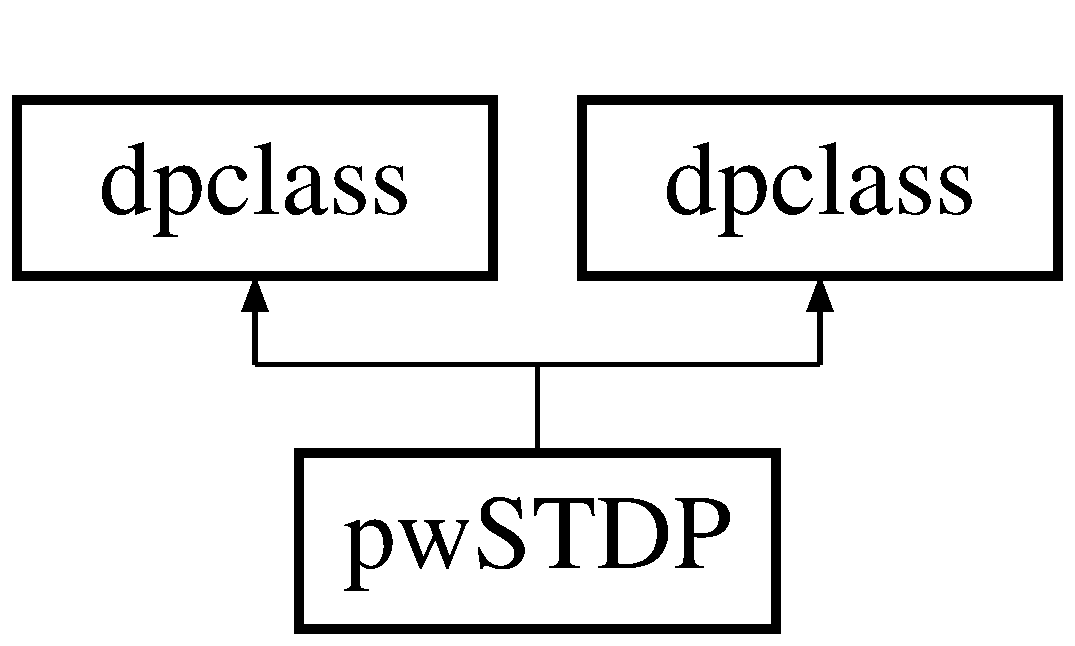
\includegraphics[height=2.000000cm]{d0/dba/classpwSTDP}
\end{center}
\end{figure}
\subsection*{Public Member Functions}
\begin{DoxyCompactItemize}
\item 
float \hyperlink{classpwSTDP_a6c0e3e483e484f8805edd58b7fb37507}{calculate\+Derived\+Parameter} (int index, vector$<$ float $>$ pars, float dt)
\item 
float \hyperlink{classpwSTDP_a996a53e179ac03e2f4865f85befad83a}{lim0} (vector$<$ float $>$ pars, float dt)
\item 
float \hyperlink{classpwSTDP_ae9755a1032792e651f9e93954fe85bb5}{lim1} (vector$<$ float $>$ pars, float dt)
\item 
float \hyperlink{classpwSTDP_a133f3a6b781d34b20be1eb951117e9f5}{slope0} (vector$<$ float $>$ pars, float dt)
\item 
float \hyperlink{classpwSTDP_a2ddfab4a97982618adc2f706e2d58aeb}{slope1} (vector$<$ float $>$ pars, float dt)
\item 
float \hyperlink{classpwSTDP_a488fa77803291d76e4e5e62766afb087}{off0} (vector$<$ float $>$ pars, float dt)
\item 
float \hyperlink{classpwSTDP_a97f72c888ee9384dd28beb7f551fcb0e}{off1} (vector$<$ float $>$ pars, float dt)
\item 
float \hyperlink{classpwSTDP_aa019d5962f48763e9468f081d6c5c1f7}{off2} (vector$<$ float $>$ pars, float dt)
\item 
float \hyperlink{classpwSTDP_a29af7a11b93e3617d9da090cc07ad578}{calculate\+Derived\+Parameter} (int index, vector$<$ float $>$ pars, float dt=\hyperlink{SynDelaySim_8h_a943f07034774ef1261d62cd0d3d1fec9}{D\+T})
\item 
float \hyperlink{classpwSTDP_a996a53e179ac03e2f4865f85befad83a}{lim0} (vector$<$ float $>$ pars, float dt)
\item 
float \hyperlink{classpwSTDP_ae9755a1032792e651f9e93954fe85bb5}{lim1} (vector$<$ float $>$ pars, float dt)
\item 
float \hyperlink{classpwSTDP_a133f3a6b781d34b20be1eb951117e9f5}{slope0} (vector$<$ float $>$ pars, float dt)
\item 
float \hyperlink{classpwSTDP_a2ddfab4a97982618adc2f706e2d58aeb}{slope1} (vector$<$ float $>$ pars, float dt)
\item 
float \hyperlink{classpwSTDP_a488fa77803291d76e4e5e62766afb087}{off0} (vector$<$ float $>$ pars, float dt)
\item 
float \hyperlink{classpwSTDP_a97f72c888ee9384dd28beb7f551fcb0e}{off1} (vector$<$ float $>$ pars, float dt)
\item 
float \hyperlink{classpwSTDP_aa019d5962f48763e9468f081d6c5c1f7}{off2} (vector$<$ float $>$ pars, float dt)
\end{DoxyCompactItemize}


\subsection{Detailed Description}
T\+O\+D\+O This class definition may be code-\/generated in a future release. 

This class defines derived parameters for the learn1synapse standard weightupdate model 

\subsection{Member Function Documentation}
\hypertarget{classpwSTDP_a6c0e3e483e484f8805edd58b7fb37507}{\index{pw\+S\+T\+D\+P@{pw\+S\+T\+D\+P}!calculate\+Derived\+Parameter@{calculate\+Derived\+Parameter}}
\index{calculate\+Derived\+Parameter@{calculate\+Derived\+Parameter}!pw\+S\+T\+D\+P@{pw\+S\+T\+D\+P}}
\subsubsection[{calculate\+Derived\+Parameter}]{\setlength{\rightskip}{0pt plus 5cm}float pw\+S\+T\+D\+P\+::calculate\+Derived\+Parameter (
\begin{DoxyParamCaption}
\item[{int}]{index, }
\item[{vector$<$ float $>$}]{pars, }
\item[{float}]{dt}
\end{DoxyParamCaption}
)\hspace{0.3cm}{\ttfamily [inline]}, {\ttfamily [virtual]}}}\label{classpwSTDP_a6c0e3e483e484f8805edd58b7fb37507}


Reimplemented from \hyperlink{classdpclass_a4227f736c0ec826d7bda6c98e783d74a}{dpclass}.

\hypertarget{classpwSTDP_a29af7a11b93e3617d9da090cc07ad578}{\index{pw\+S\+T\+D\+P@{pw\+S\+T\+D\+P}!calculate\+Derived\+Parameter@{calculate\+Derived\+Parameter}}
\index{calculate\+Derived\+Parameter@{calculate\+Derived\+Parameter}!pw\+S\+T\+D\+P@{pw\+S\+T\+D\+P}}
\subsubsection[{calculate\+Derived\+Parameter}]{\setlength{\rightskip}{0pt plus 5cm}float pw\+S\+T\+D\+P\+::calculate\+Derived\+Parameter (
\begin{DoxyParamCaption}
\item[{int}]{index, }
\item[{vector$<$ float $>$}]{pars, }
\item[{float}]{dt = {\ttfamily {\bf D\+T}}}
\end{DoxyParamCaption}
)\hspace{0.3cm}{\ttfamily [inline]}, {\ttfamily [virtual]}}}\label{classpwSTDP_a29af7a11b93e3617d9da090cc07ad578}


Reimplemented from \hyperlink{classdpclass_a4227f736c0ec826d7bda6c98e783d74a}{dpclass}.

\hypertarget{classpwSTDP_a996a53e179ac03e2f4865f85befad83a}{\index{pw\+S\+T\+D\+P@{pw\+S\+T\+D\+P}!lim0@{lim0}}
\index{lim0@{lim0}!pw\+S\+T\+D\+P@{pw\+S\+T\+D\+P}}
\subsubsection[{lim0}]{\setlength{\rightskip}{0pt plus 5cm}float pw\+S\+T\+D\+P\+::lim0 (
\begin{DoxyParamCaption}
\item[{vector$<$ float $>$}]{pars, }
\item[{float}]{dt}
\end{DoxyParamCaption}
)\hspace{0.3cm}{\ttfamily [inline]}}}\label{classpwSTDP_a996a53e179ac03e2f4865f85befad83a}
\hypertarget{classpwSTDP_a996a53e179ac03e2f4865f85befad83a}{\index{pw\+S\+T\+D\+P@{pw\+S\+T\+D\+P}!lim0@{lim0}}
\index{lim0@{lim0}!pw\+S\+T\+D\+P@{pw\+S\+T\+D\+P}}
\subsubsection[{lim0}]{\setlength{\rightskip}{0pt plus 5cm}float pw\+S\+T\+D\+P\+::lim0 (
\begin{DoxyParamCaption}
\item[{vector$<$ float $>$}]{pars, }
\item[{float}]{dt}
\end{DoxyParamCaption}
)\hspace{0.3cm}{\ttfamily [inline]}}}\label{classpwSTDP_a996a53e179ac03e2f4865f85befad83a}
\hypertarget{classpwSTDP_ae9755a1032792e651f9e93954fe85bb5}{\index{pw\+S\+T\+D\+P@{pw\+S\+T\+D\+P}!lim1@{lim1}}
\index{lim1@{lim1}!pw\+S\+T\+D\+P@{pw\+S\+T\+D\+P}}
\subsubsection[{lim1}]{\setlength{\rightskip}{0pt plus 5cm}float pw\+S\+T\+D\+P\+::lim1 (
\begin{DoxyParamCaption}
\item[{vector$<$ float $>$}]{pars, }
\item[{float}]{dt}
\end{DoxyParamCaption}
)\hspace{0.3cm}{\ttfamily [inline]}}}\label{classpwSTDP_ae9755a1032792e651f9e93954fe85bb5}
\hypertarget{classpwSTDP_ae9755a1032792e651f9e93954fe85bb5}{\index{pw\+S\+T\+D\+P@{pw\+S\+T\+D\+P}!lim1@{lim1}}
\index{lim1@{lim1}!pw\+S\+T\+D\+P@{pw\+S\+T\+D\+P}}
\subsubsection[{lim1}]{\setlength{\rightskip}{0pt plus 5cm}float pw\+S\+T\+D\+P\+::lim1 (
\begin{DoxyParamCaption}
\item[{vector$<$ float $>$}]{pars, }
\item[{float}]{dt}
\end{DoxyParamCaption}
)\hspace{0.3cm}{\ttfamily [inline]}}}\label{classpwSTDP_ae9755a1032792e651f9e93954fe85bb5}
\hypertarget{classpwSTDP_a488fa77803291d76e4e5e62766afb087}{\index{pw\+S\+T\+D\+P@{pw\+S\+T\+D\+P}!off0@{off0}}
\index{off0@{off0}!pw\+S\+T\+D\+P@{pw\+S\+T\+D\+P}}
\subsubsection[{off0}]{\setlength{\rightskip}{0pt plus 5cm}float pw\+S\+T\+D\+P\+::off0 (
\begin{DoxyParamCaption}
\item[{vector$<$ float $>$}]{pars, }
\item[{float}]{dt}
\end{DoxyParamCaption}
)\hspace{0.3cm}{\ttfamily [inline]}}}\label{classpwSTDP_a488fa77803291d76e4e5e62766afb087}
\hypertarget{classpwSTDP_a488fa77803291d76e4e5e62766afb087}{\index{pw\+S\+T\+D\+P@{pw\+S\+T\+D\+P}!off0@{off0}}
\index{off0@{off0}!pw\+S\+T\+D\+P@{pw\+S\+T\+D\+P}}
\subsubsection[{off0}]{\setlength{\rightskip}{0pt plus 5cm}float pw\+S\+T\+D\+P\+::off0 (
\begin{DoxyParamCaption}
\item[{vector$<$ float $>$}]{pars, }
\item[{float}]{dt}
\end{DoxyParamCaption}
)\hspace{0.3cm}{\ttfamily [inline]}}}\label{classpwSTDP_a488fa77803291d76e4e5e62766afb087}
\hypertarget{classpwSTDP_a97f72c888ee9384dd28beb7f551fcb0e}{\index{pw\+S\+T\+D\+P@{pw\+S\+T\+D\+P}!off1@{off1}}
\index{off1@{off1}!pw\+S\+T\+D\+P@{pw\+S\+T\+D\+P}}
\subsubsection[{off1}]{\setlength{\rightskip}{0pt plus 5cm}float pw\+S\+T\+D\+P\+::off1 (
\begin{DoxyParamCaption}
\item[{vector$<$ float $>$}]{pars, }
\item[{float}]{dt}
\end{DoxyParamCaption}
)\hspace{0.3cm}{\ttfamily [inline]}}}\label{classpwSTDP_a97f72c888ee9384dd28beb7f551fcb0e}
\hypertarget{classpwSTDP_a97f72c888ee9384dd28beb7f551fcb0e}{\index{pw\+S\+T\+D\+P@{pw\+S\+T\+D\+P}!off1@{off1}}
\index{off1@{off1}!pw\+S\+T\+D\+P@{pw\+S\+T\+D\+P}}
\subsubsection[{off1}]{\setlength{\rightskip}{0pt plus 5cm}float pw\+S\+T\+D\+P\+::off1 (
\begin{DoxyParamCaption}
\item[{vector$<$ float $>$}]{pars, }
\item[{float}]{dt}
\end{DoxyParamCaption}
)\hspace{0.3cm}{\ttfamily [inline]}}}\label{classpwSTDP_a97f72c888ee9384dd28beb7f551fcb0e}
\hypertarget{classpwSTDP_aa019d5962f48763e9468f081d6c5c1f7}{\index{pw\+S\+T\+D\+P@{pw\+S\+T\+D\+P}!off2@{off2}}
\index{off2@{off2}!pw\+S\+T\+D\+P@{pw\+S\+T\+D\+P}}
\subsubsection[{off2}]{\setlength{\rightskip}{0pt plus 5cm}float pw\+S\+T\+D\+P\+::off2 (
\begin{DoxyParamCaption}
\item[{vector$<$ float $>$}]{pars, }
\item[{float}]{dt}
\end{DoxyParamCaption}
)\hspace{0.3cm}{\ttfamily [inline]}}}\label{classpwSTDP_aa019d5962f48763e9468f081d6c5c1f7}
\hypertarget{classpwSTDP_aa019d5962f48763e9468f081d6c5c1f7}{\index{pw\+S\+T\+D\+P@{pw\+S\+T\+D\+P}!off2@{off2}}
\index{off2@{off2}!pw\+S\+T\+D\+P@{pw\+S\+T\+D\+P}}
\subsubsection[{off2}]{\setlength{\rightskip}{0pt plus 5cm}float pw\+S\+T\+D\+P\+::off2 (
\begin{DoxyParamCaption}
\item[{vector$<$ float $>$}]{pars, }
\item[{float}]{dt}
\end{DoxyParamCaption}
)\hspace{0.3cm}{\ttfamily [inline]}}}\label{classpwSTDP_aa019d5962f48763e9468f081d6c5c1f7}
\hypertarget{classpwSTDP_a133f3a6b781d34b20be1eb951117e9f5}{\index{pw\+S\+T\+D\+P@{pw\+S\+T\+D\+P}!slope0@{slope0}}
\index{slope0@{slope0}!pw\+S\+T\+D\+P@{pw\+S\+T\+D\+P}}
\subsubsection[{slope0}]{\setlength{\rightskip}{0pt plus 5cm}float pw\+S\+T\+D\+P\+::slope0 (
\begin{DoxyParamCaption}
\item[{vector$<$ float $>$}]{pars, }
\item[{float}]{dt}
\end{DoxyParamCaption}
)\hspace{0.3cm}{\ttfamily [inline]}}}\label{classpwSTDP_a133f3a6b781d34b20be1eb951117e9f5}
\hypertarget{classpwSTDP_a133f3a6b781d34b20be1eb951117e9f5}{\index{pw\+S\+T\+D\+P@{pw\+S\+T\+D\+P}!slope0@{slope0}}
\index{slope0@{slope0}!pw\+S\+T\+D\+P@{pw\+S\+T\+D\+P}}
\subsubsection[{slope0}]{\setlength{\rightskip}{0pt plus 5cm}float pw\+S\+T\+D\+P\+::slope0 (
\begin{DoxyParamCaption}
\item[{vector$<$ float $>$}]{pars, }
\item[{float}]{dt}
\end{DoxyParamCaption}
)\hspace{0.3cm}{\ttfamily [inline]}}}\label{classpwSTDP_a133f3a6b781d34b20be1eb951117e9f5}
\hypertarget{classpwSTDP_a2ddfab4a97982618adc2f706e2d58aeb}{\index{pw\+S\+T\+D\+P@{pw\+S\+T\+D\+P}!slope1@{slope1}}
\index{slope1@{slope1}!pw\+S\+T\+D\+P@{pw\+S\+T\+D\+P}}
\subsubsection[{slope1}]{\setlength{\rightskip}{0pt plus 5cm}float pw\+S\+T\+D\+P\+::slope1 (
\begin{DoxyParamCaption}
\item[{vector$<$ float $>$}]{pars, }
\item[{float}]{dt}
\end{DoxyParamCaption}
)\hspace{0.3cm}{\ttfamily [inline]}}}\label{classpwSTDP_a2ddfab4a97982618adc2f706e2d58aeb}
\hypertarget{classpwSTDP_a2ddfab4a97982618adc2f706e2d58aeb}{\index{pw\+S\+T\+D\+P@{pw\+S\+T\+D\+P}!slope1@{slope1}}
\index{slope1@{slope1}!pw\+S\+T\+D\+P@{pw\+S\+T\+D\+P}}
\subsubsection[{slope1}]{\setlength{\rightskip}{0pt plus 5cm}float pw\+S\+T\+D\+P\+::slope1 (
\begin{DoxyParamCaption}
\item[{vector$<$ float $>$}]{pars, }
\item[{float}]{dt}
\end{DoxyParamCaption}
)\hspace{0.3cm}{\ttfamily [inline]}}}\label{classpwSTDP_a2ddfab4a97982618adc2f706e2d58aeb}


The documentation for this class was generated from the following files\+:\begin{DoxyCompactItemize}
\item 
lib/include/\hyperlink{utils_8h}{utils.\+h}\item 
tmp/model/\hyperlink{tmp_2model_2MBody__userdef_8cc}{M\+Body\+\_\+userdef.\+cc}\end{DoxyCompactItemize}

\hypertarget{classpwSTDP__userdef}{\section{pw\+S\+T\+D\+P\+\_\+userdef Class Reference}
\label{classpwSTDP__userdef}\index{pw\+S\+T\+D\+P\+\_\+userdef@{pw\+S\+T\+D\+P\+\_\+userdef}}
}


T\+O\+D\+O This class definition may be code-\/generated in a future release.  


Inheritance diagram for pw\+S\+T\+D\+P\+\_\+userdef\+:\begin{figure}[H]
\begin{center}
\leavevmode
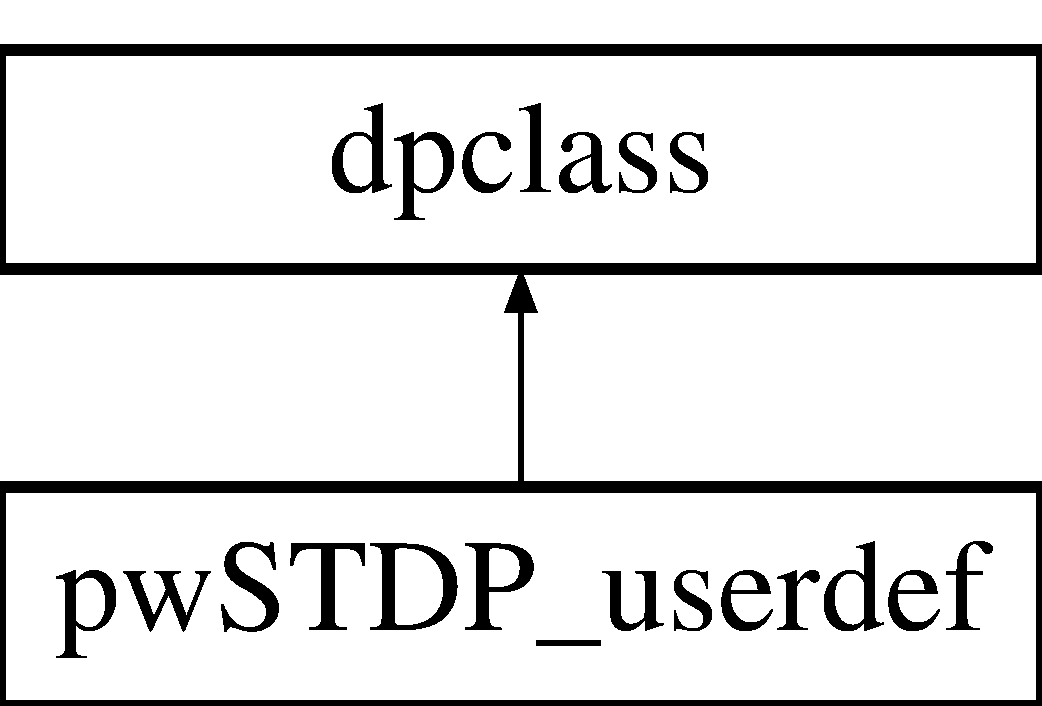
\includegraphics[height=2.000000cm]{dd/d4e/classpwSTDP__userdef}
\end{center}
\end{figure}
\subsection*{Public Member Functions}
\begin{DoxyCompactItemize}
\item 
float \hyperlink{classpwSTDP__userdef_ab97adaaca41c96af7bcb70cde27f36cf}{calculate\+Derived\+Parameter} (int index, vector$<$ float $>$ pars, float dt=\hyperlink{SynDelaySim_8h_a943f07034774ef1261d62cd0d3d1fec9}{D\+T})
\item 
float \hyperlink{classpwSTDP__userdef_a649e7e3b89a6e25d1c967c85256be22b}{lim0} (vector$<$ float $>$ pars, float dt)
\item 
float \hyperlink{classpwSTDP__userdef_a98ed2b584c1e81b3e2a6b5620d6b3e2b}{lim1} (vector$<$ float $>$ pars, float dt)
\item 
float \hyperlink{classpwSTDP__userdef_ade34631db70b55575170413dd9b57cd0}{slope0} (vector$<$ float $>$ pars, float dt)
\item 
float \hyperlink{classpwSTDP__userdef_a3a84bdf1197c357c3e7623bee86d42d6}{slope1} (vector$<$ float $>$ pars, float dt)
\item 
float \hyperlink{classpwSTDP__userdef_a45894552b5ce5311656444c4350c6a83}{off0} (vector$<$ float $>$ pars, float dt)
\item 
float \hyperlink{classpwSTDP__userdef_a07081d6b97c97073e9c65f48f7a2698b}{off1} (vector$<$ float $>$ pars, float dt)
\item 
float \hyperlink{classpwSTDP__userdef_a20a787ad267031b280618afc0646dc15}{off2} (vector$<$ float $>$ pars, float dt)
\end{DoxyCompactItemize}


\subsection{Detailed Description}
T\+O\+D\+O This class definition may be code-\/generated in a future release. 

\subsection{Member Function Documentation}
\hypertarget{classpwSTDP__userdef_ab97adaaca41c96af7bcb70cde27f36cf}{\index{pw\+S\+T\+D\+P\+\_\+userdef@{pw\+S\+T\+D\+P\+\_\+userdef}!calculate\+Derived\+Parameter@{calculate\+Derived\+Parameter}}
\index{calculate\+Derived\+Parameter@{calculate\+Derived\+Parameter}!pw\+S\+T\+D\+P\+\_\+userdef@{pw\+S\+T\+D\+P\+\_\+userdef}}
\subsubsection[{calculate\+Derived\+Parameter}]{\setlength{\rightskip}{0pt plus 5cm}float pw\+S\+T\+D\+P\+\_\+userdef\+::calculate\+Derived\+Parameter (
\begin{DoxyParamCaption}
\item[{int}]{index, }
\item[{vector$<$ float $>$}]{pars, }
\item[{float}]{dt = {\ttfamily {\bf D\+T}}}
\end{DoxyParamCaption}
)\hspace{0.3cm}{\ttfamily [inline]}, {\ttfamily [virtual]}}}\label{classpwSTDP__userdef_ab97adaaca41c96af7bcb70cde27f36cf}


Reimplemented from \hyperlink{classdpclass_a4227f736c0ec826d7bda6c98e783d74a}{dpclass}.

\hypertarget{classpwSTDP__userdef_a649e7e3b89a6e25d1c967c85256be22b}{\index{pw\+S\+T\+D\+P\+\_\+userdef@{pw\+S\+T\+D\+P\+\_\+userdef}!lim0@{lim0}}
\index{lim0@{lim0}!pw\+S\+T\+D\+P\+\_\+userdef@{pw\+S\+T\+D\+P\+\_\+userdef}}
\subsubsection[{lim0}]{\setlength{\rightskip}{0pt plus 5cm}float pw\+S\+T\+D\+P\+\_\+userdef\+::lim0 (
\begin{DoxyParamCaption}
\item[{vector$<$ float $>$}]{pars, }
\item[{float}]{dt}
\end{DoxyParamCaption}
)\hspace{0.3cm}{\ttfamily [inline]}}}\label{classpwSTDP__userdef_a649e7e3b89a6e25d1c967c85256be22b}
\hypertarget{classpwSTDP__userdef_a98ed2b584c1e81b3e2a6b5620d6b3e2b}{\index{pw\+S\+T\+D\+P\+\_\+userdef@{pw\+S\+T\+D\+P\+\_\+userdef}!lim1@{lim1}}
\index{lim1@{lim1}!pw\+S\+T\+D\+P\+\_\+userdef@{pw\+S\+T\+D\+P\+\_\+userdef}}
\subsubsection[{lim1}]{\setlength{\rightskip}{0pt plus 5cm}float pw\+S\+T\+D\+P\+\_\+userdef\+::lim1 (
\begin{DoxyParamCaption}
\item[{vector$<$ float $>$}]{pars, }
\item[{float}]{dt}
\end{DoxyParamCaption}
)\hspace{0.3cm}{\ttfamily [inline]}}}\label{classpwSTDP__userdef_a98ed2b584c1e81b3e2a6b5620d6b3e2b}
\hypertarget{classpwSTDP__userdef_a45894552b5ce5311656444c4350c6a83}{\index{pw\+S\+T\+D\+P\+\_\+userdef@{pw\+S\+T\+D\+P\+\_\+userdef}!off0@{off0}}
\index{off0@{off0}!pw\+S\+T\+D\+P\+\_\+userdef@{pw\+S\+T\+D\+P\+\_\+userdef}}
\subsubsection[{off0}]{\setlength{\rightskip}{0pt plus 5cm}float pw\+S\+T\+D\+P\+\_\+userdef\+::off0 (
\begin{DoxyParamCaption}
\item[{vector$<$ float $>$}]{pars, }
\item[{float}]{dt}
\end{DoxyParamCaption}
)\hspace{0.3cm}{\ttfamily [inline]}}}\label{classpwSTDP__userdef_a45894552b5ce5311656444c4350c6a83}
\hypertarget{classpwSTDP__userdef_a07081d6b97c97073e9c65f48f7a2698b}{\index{pw\+S\+T\+D\+P\+\_\+userdef@{pw\+S\+T\+D\+P\+\_\+userdef}!off1@{off1}}
\index{off1@{off1}!pw\+S\+T\+D\+P\+\_\+userdef@{pw\+S\+T\+D\+P\+\_\+userdef}}
\subsubsection[{off1}]{\setlength{\rightskip}{0pt plus 5cm}float pw\+S\+T\+D\+P\+\_\+userdef\+::off1 (
\begin{DoxyParamCaption}
\item[{vector$<$ float $>$}]{pars, }
\item[{float}]{dt}
\end{DoxyParamCaption}
)\hspace{0.3cm}{\ttfamily [inline]}}}\label{classpwSTDP__userdef_a07081d6b97c97073e9c65f48f7a2698b}
\hypertarget{classpwSTDP__userdef_a20a787ad267031b280618afc0646dc15}{\index{pw\+S\+T\+D\+P\+\_\+userdef@{pw\+S\+T\+D\+P\+\_\+userdef}!off2@{off2}}
\index{off2@{off2}!pw\+S\+T\+D\+P\+\_\+userdef@{pw\+S\+T\+D\+P\+\_\+userdef}}
\subsubsection[{off2}]{\setlength{\rightskip}{0pt plus 5cm}float pw\+S\+T\+D\+P\+\_\+userdef\+::off2 (
\begin{DoxyParamCaption}
\item[{vector$<$ float $>$}]{pars, }
\item[{float}]{dt}
\end{DoxyParamCaption}
)\hspace{0.3cm}{\ttfamily [inline]}}}\label{classpwSTDP__userdef_a20a787ad267031b280618afc0646dc15}
\hypertarget{classpwSTDP__userdef_ade34631db70b55575170413dd9b57cd0}{\index{pw\+S\+T\+D\+P\+\_\+userdef@{pw\+S\+T\+D\+P\+\_\+userdef}!slope0@{slope0}}
\index{slope0@{slope0}!pw\+S\+T\+D\+P\+\_\+userdef@{pw\+S\+T\+D\+P\+\_\+userdef}}
\subsubsection[{slope0}]{\setlength{\rightskip}{0pt plus 5cm}float pw\+S\+T\+D\+P\+\_\+userdef\+::slope0 (
\begin{DoxyParamCaption}
\item[{vector$<$ float $>$}]{pars, }
\item[{float}]{dt}
\end{DoxyParamCaption}
)\hspace{0.3cm}{\ttfamily [inline]}}}\label{classpwSTDP__userdef_ade34631db70b55575170413dd9b57cd0}
\hypertarget{classpwSTDP__userdef_a3a84bdf1197c357c3e7623bee86d42d6}{\index{pw\+S\+T\+D\+P\+\_\+userdef@{pw\+S\+T\+D\+P\+\_\+userdef}!slope1@{slope1}}
\index{slope1@{slope1}!pw\+S\+T\+D\+P\+\_\+userdef@{pw\+S\+T\+D\+P\+\_\+userdef}}
\subsubsection[{slope1}]{\setlength{\rightskip}{0pt plus 5cm}float pw\+S\+T\+D\+P\+\_\+userdef\+::slope1 (
\begin{DoxyParamCaption}
\item[{vector$<$ float $>$}]{pars, }
\item[{float}]{dt}
\end{DoxyParamCaption}
)\hspace{0.3cm}{\ttfamily [inline]}}}\label{classpwSTDP__userdef_a3a84bdf1197c357c3e7623bee86d42d6}


The documentation for this class was generated from the following file\+:\begin{DoxyCompactItemize}
\item 
userproject/\+M\+Body\+\_\+userdef\+\_\+project/model/\hyperlink{userproject_2MBody__userdef__project_2model_2MBody__userdef_8cc}{M\+Body\+\_\+userdef.\+cc}\end{DoxyCompactItemize}

\hypertarget{classrandomGauss}{\section{random\+Gauss Class Reference}
\label{classrandomGauss}\index{random\+Gauss@{random\+Gauss}}
}


Class random Gauss encapsulates the methods for generating random neumbers with Gaussian distribution.  




{\ttfamily \#include $<$gauss.\+h$>$}

\subsection*{Public Member Functions}
\begin{DoxyCompactItemize}
\item 
\hyperlink{classrandomGauss_aadeaf98f80482a1515e0faf0bb0f3094}{random\+Gauss} ()
\begin{DoxyCompactList}\small\item\em Constructor for the Gaussian random number generator class without giving explicit seeds. \end{DoxyCompactList}\item 
\hyperlink{classrandomGauss_ac7e74917c3456acef39d012b430d3438}{random\+Gauss} (unsigned long, unsigned long, unsigned long)
\begin{DoxyCompactList}\small\item\em Constructor for the Gaussian random number generator class when seeds are provided explicitly. \end{DoxyCompactList}\item 
\hyperlink{classrandomGauss_a2925cbc1ccf2cfdb91e042d8b2cc373a}{$\sim$random\+Gauss} ()
\item 
double \hyperlink{classrandomGauss_a69a70b10bc65de93f60bfb1c02a16daf}{n} ()
\begin{DoxyCompactList}\small\item\em Method for obtaining a random number with Gaussian distribution. \end{DoxyCompactList}\end{DoxyCompactItemize}


\subsection{Detailed Description}
Class random Gauss encapsulates the methods for generating random neumbers with Gaussian distribution. 

A random number from a Gaussian distribution of mean 0 and standard deviation 1 is obtained by calling the method \hyperlink{classrandomGauss_a69a70b10bc65de93f60bfb1c02a16daf}{random\+Gauss\+::n()}. 

\subsection{Constructor \& Destructor Documentation}
\hypertarget{classrandomGauss_aadeaf98f80482a1515e0faf0bb0f3094}{\index{random\+Gauss@{random\+Gauss}!random\+Gauss@{random\+Gauss}}
\index{random\+Gauss@{random\+Gauss}!random\+Gauss@{random\+Gauss}}
\subsubsection[{random\+Gauss}]{\setlength{\rightskip}{0pt plus 5cm}random\+Gauss\+::random\+Gauss (
\begin{DoxyParamCaption}
{}
\end{DoxyParamCaption}
)\hspace{0.3cm}{\ttfamily [explicit]}}}\label{classrandomGauss_aadeaf98f80482a1515e0faf0bb0f3094}


Constructor for the Gaussian random number generator class without giving explicit seeds. 

The seeds for random number generation are generated from the internal clock of the computer during execution. \hypertarget{classrandomGauss_ac7e74917c3456acef39d012b430d3438}{\index{random\+Gauss@{random\+Gauss}!random\+Gauss@{random\+Gauss}}
\index{random\+Gauss@{random\+Gauss}!random\+Gauss@{random\+Gauss}}
\subsubsection[{random\+Gauss}]{\setlength{\rightskip}{0pt plus 5cm}random\+Gauss\+::random\+Gauss (
\begin{DoxyParamCaption}
\item[{unsigned long}]{seed1, }
\item[{unsigned long}]{seed2, }
\item[{unsigned long}]{seed3}
\end{DoxyParamCaption}
)}}\label{classrandomGauss_ac7e74917c3456acef39d012b430d3438}


Constructor for the Gaussian random number generator class when seeds are provided explicitly. 

The seeds are three arbitrary unsigned long integers. \hypertarget{classrandomGauss_a2925cbc1ccf2cfdb91e042d8b2cc373a}{\index{random\+Gauss@{random\+Gauss}!````~random\+Gauss@{$\sim$random\+Gauss}}
\index{````~random\+Gauss@{$\sim$random\+Gauss}!random\+Gauss@{random\+Gauss}}
\subsubsection[{$\sim$random\+Gauss}]{\setlength{\rightskip}{0pt plus 5cm}random\+Gauss\+::$\sim$random\+Gauss (
\begin{DoxyParamCaption}
{}
\end{DoxyParamCaption}
)\hspace{0.3cm}{\ttfamily [inline]}}}\label{classrandomGauss_a2925cbc1ccf2cfdb91e042d8b2cc373a}


\subsection{Member Function Documentation}
\hypertarget{classrandomGauss_a69a70b10bc65de93f60bfb1c02a16daf}{\index{random\+Gauss@{random\+Gauss}!n@{n}}
\index{n@{n}!random\+Gauss@{random\+Gauss}}
\subsubsection[{n}]{\setlength{\rightskip}{0pt plus 5cm}double random\+Gauss\+::n (
\begin{DoxyParamCaption}
{}
\end{DoxyParamCaption}
)}}\label{classrandomGauss_a69a70b10bc65de93f60bfb1c02a16daf}


Method for obtaining a random number with Gaussian distribution. 

Function for generating a pseudo random number from a Gaussian distribution. 

The documentation for this class was generated from the following files\+:\begin{DoxyCompactItemize}
\item 
lib/include/numlib/\hyperlink{gauss_8h}{gauss.\+h}\item 
lib/include/numlib/\hyperlink{gauss_8cc}{gauss.\+cc}\end{DoxyCompactItemize}

\hypertarget{classrandomGen}{\section{random\+Gen Class Reference}
\label{classrandomGen}\index{random\+Gen@{random\+Gen}}
}


Class \hyperlink{classrandomGen}{random\+Gen} which implements the I\+S\+A\+A\+C random number generator for uniformely distributed random numbers.  




{\ttfamily \#include $<$random\+Gen.\+h$>$}

\subsection*{Public Member Functions}
\begin{DoxyCompactItemize}
\item 
\hyperlink{classrandomGen_ada03051a500718832b829f7d6f699028}{random\+Gen} ()
\begin{DoxyCompactList}\small\item\em Constructor for the I\+S\+A\+A\+C random number generator class without giving explicit seeds. \end{DoxyCompactList}\item 
\hyperlink{classrandomGen_aaec36a636be1fbdffed0c6775566e739}{random\+Gen} (unsigned long, unsigned long, unsigned long)
\begin{DoxyCompactList}\small\item\em Constructor for the Gaussian random number generator class when seeds are provided explicitly. \end{DoxyCompactList}\item 
\hyperlink{classrandomGen_aff27fbad3b28842484acd1422c41ca66}{$\sim$random\+Gen} ()
\item 
double \hyperlink{classrandomGen_a38b3e42d3a1b00f069a88f0dcceed43d}{n} ()
\begin{DoxyCompactList}\small\item\em Method to obtain a random number from a uniform ditribution on \mbox{[}0,1\mbox{]}. \end{DoxyCompactList}\end{DoxyCompactItemize}


\subsection{Detailed Description}
Class \hyperlink{classrandomGen}{random\+Gen} which implements the I\+S\+A\+A\+C random number generator for uniformely distributed random numbers. 

The random number generator initializes with system timea or explicit seeds and returns a random number according to a uniform distribution on \mbox{[}0,1\mbox{]}; making use of the I\+S\+A\+A\+C random number generator; C++ Implementation by Quinn Tyler Jackson of the R\+G invented by Bob Jenkins Jr. 

\subsection{Constructor \& Destructor Documentation}
\hypertarget{classrandomGen_ada03051a500718832b829f7d6f699028}{\index{random\+Gen@{random\+Gen}!random\+Gen@{random\+Gen}}
\index{random\+Gen@{random\+Gen}!random\+Gen@{random\+Gen}}
\subsubsection[{random\+Gen}]{\setlength{\rightskip}{0pt plus 5cm}random\+Gen\+::random\+Gen (
\begin{DoxyParamCaption}
{}
\end{DoxyParamCaption}
)\hspace{0.3cm}{\ttfamily [explicit]}}}\label{classrandomGen_ada03051a500718832b829f7d6f699028}


Constructor for the I\+S\+A\+A\+C random number generator class without giving explicit seeds. 

The seeds for random number generation are generated from the internal clock of the computer during execution. \hypertarget{classrandomGen_aaec36a636be1fbdffed0c6775566e739}{\index{random\+Gen@{random\+Gen}!random\+Gen@{random\+Gen}}
\index{random\+Gen@{random\+Gen}!random\+Gen@{random\+Gen}}
\subsubsection[{random\+Gen}]{\setlength{\rightskip}{0pt plus 5cm}random\+Gen\+::random\+Gen (
\begin{DoxyParamCaption}
\item[{unsigned long}]{seed1, }
\item[{unsigned long}]{seed2, }
\item[{unsigned long}]{seed3}
\end{DoxyParamCaption}
)}}\label{classrandomGen_aaec36a636be1fbdffed0c6775566e739}


Constructor for the Gaussian random number generator class when seeds are provided explicitly. 

The seeds are three arbitrary unsigned long integers. \hypertarget{classrandomGen_aff27fbad3b28842484acd1422c41ca66}{\index{random\+Gen@{random\+Gen}!````~random\+Gen@{$\sim$random\+Gen}}
\index{````~random\+Gen@{$\sim$random\+Gen}!random\+Gen@{random\+Gen}}
\subsubsection[{$\sim$random\+Gen}]{\setlength{\rightskip}{0pt plus 5cm}random\+Gen\+::$\sim$random\+Gen (
\begin{DoxyParamCaption}
{}
\end{DoxyParamCaption}
)\hspace{0.3cm}{\ttfamily [inline]}}}\label{classrandomGen_aff27fbad3b28842484acd1422c41ca66}


\subsection{Member Function Documentation}
\hypertarget{classrandomGen_a38b3e42d3a1b00f069a88f0dcceed43d}{\index{random\+Gen@{random\+Gen}!n@{n}}
\index{n@{n}!random\+Gen@{random\+Gen}}
\subsubsection[{n}]{\setlength{\rightskip}{0pt plus 5cm}double random\+Gen\+::n (
\begin{DoxyParamCaption}
{}
\end{DoxyParamCaption}
)}}\label{classrandomGen_a38b3e42d3a1b00f069a88f0dcceed43d}


Method to obtain a random number from a uniform ditribution on \mbox{[}0,1\mbox{]}. 

Function for generating a pseudo random number from a uniform distribution on the interval \mbox{[}0,1\mbox{]}. 

The documentation for this class was generated from the following files\+:\begin{DoxyCompactItemize}
\item 
lib/include/numlib/\hyperlink{randomGen_8h}{random\+Gen.\+h}\item 
lib/include/numlib/\hyperlink{randomGen_8cc}{random\+Gen.\+cc}\end{DoxyCompactItemize}

\hypertarget{classrulkovdp}{\section{rulkovdp Class Reference}
\label{classrulkovdp}\index{rulkovdp@{rulkovdp}}
}


Class defining the dependent parameters of teh Rulkov map neuron.  




{\ttfamily \#include $<$utils.\+h$>$}

Inheritance diagram for rulkovdp\+:\begin{figure}[H]
\begin{center}
\leavevmode
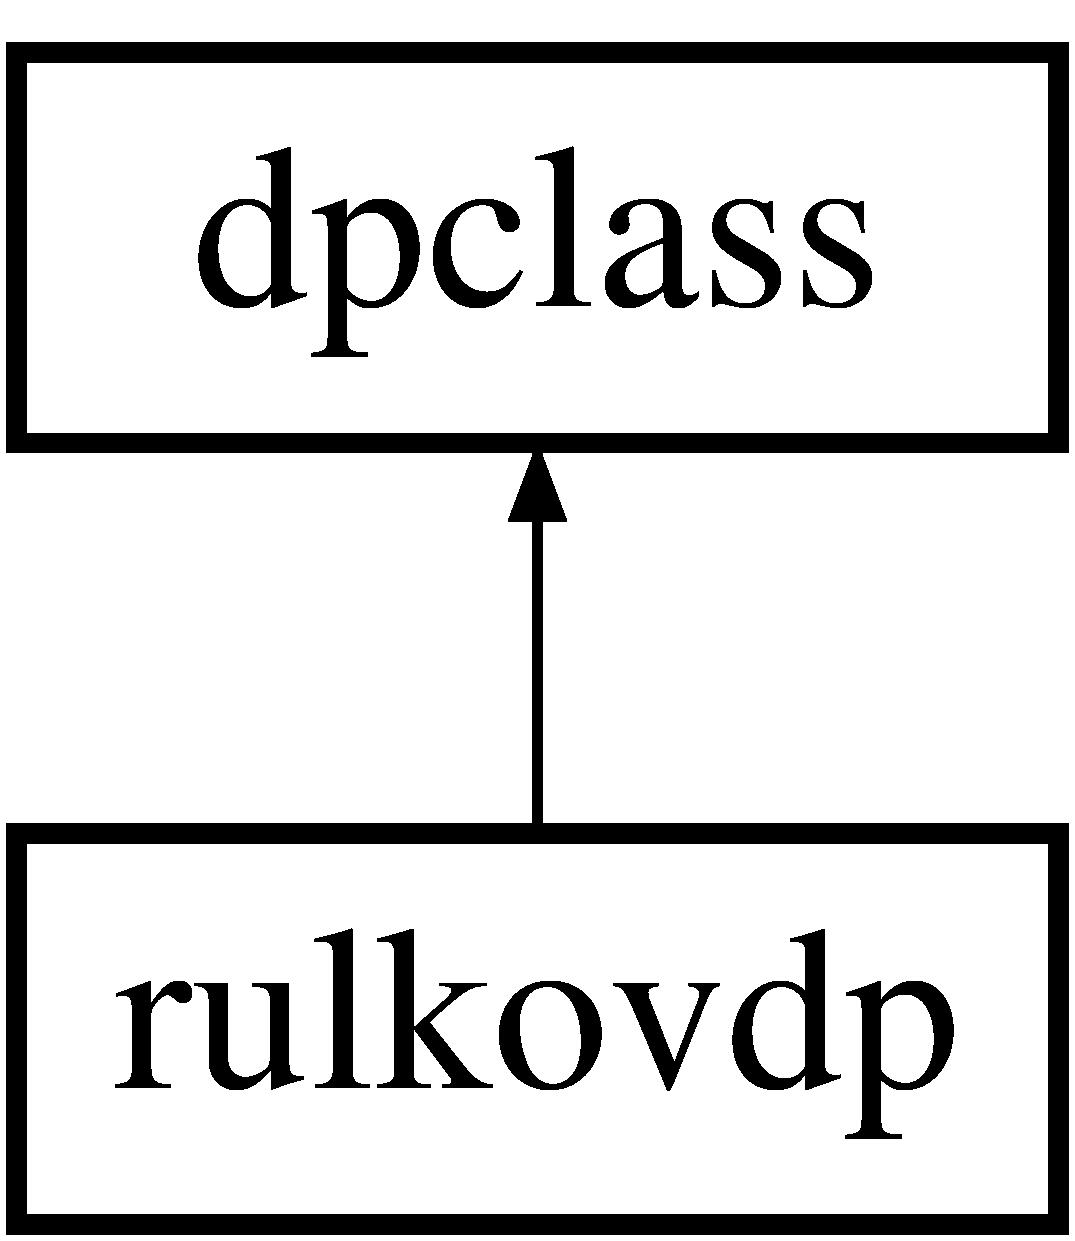
\includegraphics[height=2.000000cm]{d6/d9e/classrulkovdp}
\end{center}
\end{figure}
\subsection*{Public Member Functions}
\begin{DoxyCompactItemize}
\item 
float \hyperlink{classrulkovdp_ac05fee8df961da95972c7343e677660e}{calculate\+Derived\+Parameter} (int index, vector$<$ float $>$ pars, float dt=1.\+0)
\item 
float \hyperlink{classrulkovdp_ab5acc4cf3debc79b90c4deeb882853ef}{ip0} (vector$<$ float $>$ pars)
\item 
float \hyperlink{classrulkovdp_a17547ab749f415b453fda7585317df32}{ip1} (vector$<$ float $>$ pars)
\item 
float \hyperlink{classrulkovdp_a9a264ffaa444a7182027a4242f1d8873}{ip2} (vector$<$ float $>$ pars)
\end{DoxyCompactItemize}


\subsection{Detailed Description}
Class defining the dependent parameters of teh Rulkov map neuron. 

\subsection{Member Function Documentation}
\hypertarget{classrulkovdp_ac05fee8df961da95972c7343e677660e}{\index{rulkovdp@{rulkovdp}!calculate\+Derived\+Parameter@{calculate\+Derived\+Parameter}}
\index{calculate\+Derived\+Parameter@{calculate\+Derived\+Parameter}!rulkovdp@{rulkovdp}}
\subsubsection[{calculate\+Derived\+Parameter}]{\setlength{\rightskip}{0pt plus 5cm}float rulkovdp\+::calculate\+Derived\+Parameter (
\begin{DoxyParamCaption}
\item[{int}]{index, }
\item[{vector$<$ float $>$}]{pars, }
\item[{float}]{dt = {\ttfamily 1.0}}
\end{DoxyParamCaption}
)\hspace{0.3cm}{\ttfamily [inline]}, {\ttfamily [virtual]}}}\label{classrulkovdp_ac05fee8df961da95972c7343e677660e}


Reimplemented from \hyperlink{classdpclass_a4227f736c0ec826d7bda6c98e783d74a}{dpclass}.

\hypertarget{classrulkovdp_ab5acc4cf3debc79b90c4deeb882853ef}{\index{rulkovdp@{rulkovdp}!ip0@{ip0}}
\index{ip0@{ip0}!rulkovdp@{rulkovdp}}
\subsubsection[{ip0}]{\setlength{\rightskip}{0pt plus 5cm}float rulkovdp\+::ip0 (
\begin{DoxyParamCaption}
\item[{vector$<$ float $>$}]{pars}
\end{DoxyParamCaption}
)\hspace{0.3cm}{\ttfamily [inline]}}}\label{classrulkovdp_ab5acc4cf3debc79b90c4deeb882853ef}
\hypertarget{classrulkovdp_a17547ab749f415b453fda7585317df32}{\index{rulkovdp@{rulkovdp}!ip1@{ip1}}
\index{ip1@{ip1}!rulkovdp@{rulkovdp}}
\subsubsection[{ip1}]{\setlength{\rightskip}{0pt plus 5cm}float rulkovdp\+::ip1 (
\begin{DoxyParamCaption}
\item[{vector$<$ float $>$}]{pars}
\end{DoxyParamCaption}
)\hspace{0.3cm}{\ttfamily [inline]}}}\label{classrulkovdp_a17547ab749f415b453fda7585317df32}
\hypertarget{classrulkovdp_a9a264ffaa444a7182027a4242f1d8873}{\index{rulkovdp@{rulkovdp}!ip2@{ip2}}
\index{ip2@{ip2}!rulkovdp@{rulkovdp}}
\subsubsection[{ip2}]{\setlength{\rightskip}{0pt plus 5cm}float rulkovdp\+::ip2 (
\begin{DoxyParamCaption}
\item[{vector$<$ float $>$}]{pars}
\end{DoxyParamCaption}
)\hspace{0.3cm}{\ttfamily [inline]}}}\label{classrulkovdp_a9a264ffaa444a7182027a4242f1d8873}


The documentation for this class was generated from the following file\+:\begin{DoxyCompactItemize}
\item 
lib/include/\hyperlink{utils_8h}{utils.\+h}\end{DoxyCompactItemize}

\hypertarget{classstdRG}{\section{std\+R\+G Class Reference}
\label{classstdRG}\index{std\+R\+G@{std\+R\+G}}
}


{\ttfamily \#include $<$random\+Gen.\+h$>$}

\subsection*{Public Member Functions}
\begin{DoxyCompactItemize}
\item 
\hyperlink{classstdRG_a49cecf58206a2a7f6e7994357672f5de}{std\+R\+G} ()
\begin{DoxyCompactList}\small\item\em Constructor of the standard random number generator class without explicit seed. \end{DoxyCompactList}\item 
\hyperlink{classstdRG_ad8bc46a003776b139f3684b91cae21b6}{std\+R\+G} (unsigned int)
\begin{DoxyCompactList}\small\item\em Constructor of the standard random number generator class with explicit seed. \end{DoxyCompactList}\item 
\hyperlink{classstdRG_a0bbc8b513176fbf0fdadb5b568222ffe}{$\sim$std\+R\+G} ()
\item 
double \hyperlink{classstdRG_ab2b84f84f234df06a63aec2e69351fdd}{n} ()
\begin{DoxyCompactList}\small\item\em Method to generate a uniform random number. \end{DoxyCompactList}\item 
unsigned long \hyperlink{classstdRG_a7abd7966eb13e25de120e4ef05e4e877}{nlong} ()
\end{DoxyCompactItemize}


\subsection{Constructor \& Destructor Documentation}
\hypertarget{classstdRG_a49cecf58206a2a7f6e7994357672f5de}{\index{std\+R\+G@{std\+R\+G}!std\+R\+G@{std\+R\+G}}
\index{std\+R\+G@{std\+R\+G}!std\+R\+G@{std\+R\+G}}
\subsubsection[{std\+R\+G}]{\setlength{\rightskip}{0pt plus 5cm}std\+R\+G\+::std\+R\+G (
\begin{DoxyParamCaption}
{}
\end{DoxyParamCaption}
)\hspace{0.3cm}{\ttfamily [explicit]}}}\label{classstdRG_a49cecf58206a2a7f6e7994357672f5de}


Constructor of the standard random number generator class without explicit seed. 

The seed is taken from teh internal clock of the computer. \hypertarget{classstdRG_ad8bc46a003776b139f3684b91cae21b6}{\index{std\+R\+G@{std\+R\+G}!std\+R\+G@{std\+R\+G}}
\index{std\+R\+G@{std\+R\+G}!std\+R\+G@{std\+R\+G}}
\subsubsection[{std\+R\+G}]{\setlength{\rightskip}{0pt plus 5cm}std\+R\+G\+::std\+R\+G (
\begin{DoxyParamCaption}
\item[{unsigned int}]{seed}
\end{DoxyParamCaption}
)}}\label{classstdRG_ad8bc46a003776b139f3684b91cae21b6}


Constructor of the standard random number generator class with explicit seed. 

The seed is an arbitrary unsigned int \hypertarget{classstdRG_a0bbc8b513176fbf0fdadb5b568222ffe}{\index{std\+R\+G@{std\+R\+G}!````~std\+R\+G@{$\sim$std\+R\+G}}
\index{````~std\+R\+G@{$\sim$std\+R\+G}!std\+R\+G@{std\+R\+G}}
\subsubsection[{$\sim$std\+R\+G}]{\setlength{\rightskip}{0pt plus 5cm}std\+R\+G\+::$\sim$std\+R\+G (
\begin{DoxyParamCaption}
{}
\end{DoxyParamCaption}
)\hspace{0.3cm}{\ttfamily [inline]}}}\label{classstdRG_a0bbc8b513176fbf0fdadb5b568222ffe}


\subsection{Member Function Documentation}
\hypertarget{classstdRG_ab2b84f84f234df06a63aec2e69351fdd}{\index{std\+R\+G@{std\+R\+G}!n@{n}}
\index{n@{n}!std\+R\+G@{std\+R\+G}}
\subsubsection[{n}]{\setlength{\rightskip}{0pt plus 5cm}double std\+R\+G\+::n (
\begin{DoxyParamCaption}
{}
\end{DoxyParamCaption}
)}}\label{classstdRG_ab2b84f84f234df06a63aec2e69351fdd}


Method to generate a uniform random number. 

The moethod is a wrapper for the C function rand() and returns a pseudo random number in the interval \mbox{[}0,1\mbox{[} \hypertarget{classstdRG_a7abd7966eb13e25de120e4ef05e4e877}{\index{std\+R\+G@{std\+R\+G}!nlong@{nlong}}
\index{nlong@{nlong}!std\+R\+G@{std\+R\+G}}
\subsubsection[{nlong}]{\setlength{\rightskip}{0pt plus 5cm}unsigned long std\+R\+G\+::nlong (
\begin{DoxyParamCaption}
{}
\end{DoxyParamCaption}
)}}\label{classstdRG_a7abd7966eb13e25de120e4ef05e4e877}


The documentation for this class was generated from the following files\+:\begin{DoxyCompactItemize}
\item 
lib/include/numlib/\hyperlink{randomGen_8h}{random\+Gen.\+h}\item 
lib/include/numlib/\hyperlink{randomGen_8cc}{random\+Gen.\+cc}\end{DoxyCompactItemize}

\hypertarget{structstopWatch}{\section{stop\+Watch Struct Reference}
\label{structstopWatch}\index{stop\+Watch@{stop\+Watch}}
}


{\ttfamily \#include $<$hr\+\_\+time.\+h$>$}

\subsection*{Public Attributes}
\begin{DoxyCompactItemize}
\item 
timeval \hyperlink{structstopWatch_aec7dc4d315b26843c8d5455afb531441}{start}
\item 
timeval \hyperlink{structstopWatch_ab6353f18737a93dda37f42faee1a808c}{stop}
\end{DoxyCompactItemize}


\subsection{Member Data Documentation}
\hypertarget{structstopWatch_aec7dc4d315b26843c8d5455afb531441}{\index{stop\+Watch@{stop\+Watch}!start@{start}}
\index{start@{start}!stop\+Watch@{stop\+Watch}}
\subsubsection[{start}]{\setlength{\rightskip}{0pt plus 5cm}timeval stop\+Watch\+::start}}\label{structstopWatch_aec7dc4d315b26843c8d5455afb531441}
\hypertarget{structstopWatch_ab6353f18737a93dda37f42faee1a808c}{\index{stop\+Watch@{stop\+Watch}!stop@{stop}}
\index{stop@{stop}!stop\+Watch@{stop\+Watch}}
\subsubsection[{stop}]{\setlength{\rightskip}{0pt plus 5cm}timeval stop\+Watch\+::stop}}\label{structstopWatch_ab6353f18737a93dda37f42faee1a808c}


The documentation for this struct was generated from the following file\+:\begin{DoxyCompactItemize}
\item 
lib/include/\hyperlink{hr__time_8h}{hr\+\_\+time.\+h}\end{DoxyCompactItemize}

\hypertarget{classSynDelay}{\section{Syn\+Delay Class Reference}
\label{classSynDelay}\index{Syn\+Delay@{Syn\+Delay}}
}


{\ttfamily \#include $<$Syn\+Delay\+Sim.\+h$>$}

\subsection*{Public Member Functions}
\begin{DoxyCompactItemize}
\item 
\hyperlink{classSynDelay_aaade14bd66306666c78e8c121e44ce96}{Syn\+Delay} (bool using\+G\+P\+U)
\item 
\hyperlink{classSynDelay_ad39ace0c45d15b6beb716c9efad2312f}{$\sim$\+Syn\+Delay} ()
\item 
void \hyperlink{classSynDelay_a629ac9d73cecfb93bd4e867f15ada331}{run} (float \hyperlink{PoissonIzh__sim_8h_afea36502e9d227ff62c5fb2719a246f2}{t})
\end{DoxyCompactItemize}


\subsection{Constructor \& Destructor Documentation}
\hypertarget{classSynDelay_aaade14bd66306666c78e8c121e44ce96}{\index{Syn\+Delay@{Syn\+Delay}!Syn\+Delay@{Syn\+Delay}}
\index{Syn\+Delay@{Syn\+Delay}!Syn\+Delay@{Syn\+Delay}}
\subsubsection[{Syn\+Delay}]{\setlength{\rightskip}{0pt plus 5cm}Syn\+Delay\+::\+Syn\+Delay (
\begin{DoxyParamCaption}
\item[{bool}]{using\+G\+P\+U}
\end{DoxyParamCaption}
)}}\label{classSynDelay_aaade14bd66306666c78e8c121e44ce96}
\hypertarget{classSynDelay_ad39ace0c45d15b6beb716c9efad2312f}{\index{Syn\+Delay@{Syn\+Delay}!````~Syn\+Delay@{$\sim$\+Syn\+Delay}}
\index{````~Syn\+Delay@{$\sim$\+Syn\+Delay}!Syn\+Delay@{Syn\+Delay}}
\subsubsection[{$\sim$\+Syn\+Delay}]{\setlength{\rightskip}{0pt plus 5cm}Syn\+Delay\+::$\sim$\+Syn\+Delay (
\begin{DoxyParamCaption}
{}
\end{DoxyParamCaption}
)}}\label{classSynDelay_ad39ace0c45d15b6beb716c9efad2312f}


\subsection{Member Function Documentation}
\hypertarget{classSynDelay_a629ac9d73cecfb93bd4e867f15ada331}{\index{Syn\+Delay@{Syn\+Delay}!run@{run}}
\index{run@{run}!Syn\+Delay@{Syn\+Delay}}
\subsubsection[{run}]{\setlength{\rightskip}{0pt plus 5cm}void Syn\+Delay\+::run (
\begin{DoxyParamCaption}
\item[{float}]{t}
\end{DoxyParamCaption}
)}}\label{classSynDelay_a629ac9d73cecfb93bd4e867f15ada331}


The documentation for this class was generated from the following files\+:\begin{DoxyCompactItemize}
\item 
userproject/\+Syn\+Delay\+\_\+project/\hyperlink{SynDelaySim_8h}{Syn\+Delay\+Sim.\+h}\item 
userproject/\+Syn\+Delay\+\_\+project/\hyperlink{SynDelaySim_8cu}{Syn\+Delay\+Sim.\+cu}\end{DoxyCompactItemize}

\hypertarget{classweightUpdateModel}{\section{weight\+Update\+Model Class Reference}
\label{classweightUpdateModel}\index{weight\+Update\+Model@{weight\+Update\+Model}}
}


Structure to hold the information that defines a weightupdate model (a model of how spikes affect synaptic (and/or) (mostly) post-\/synaptic neuron variables. It also allows to define changes in response to post-\/synaptic spikes/spike-\/like events.  




{\ttfamily \#include $<$model\+Spec.\+h$>$}

\subsection*{Public Member Functions}
\begin{DoxyCompactItemize}
\item 
\hyperlink{classweightUpdateModel_ae83d9e39690aaa754ab5be7b72ca60d5}{weight\+Update\+Model} ()
\end{DoxyCompactItemize}
\subsection*{Public Attributes}
\begin{DoxyCompactItemize}
\item 
string \hyperlink{classweightUpdateModel_a6f665453175451356bbf14b9f60baed3}{sim\+Code}
\item 
string \hyperlink{classweightUpdateModel_a758cc3211ae12407583f625418dd5a89}{sim\+Code\+Evnt}
\item 
string \hyperlink{classweightUpdateModel_a9ebdfd1b336b3c40403546deb05cbfc9}{sim\+Learn\+Post}
\item 
string \hyperlink{classweightUpdateModel_acccf120c9b1307f7ee2c5bac43110be1}{evnt\+Threshold}
\item 
string \hyperlink{classweightUpdateModel_a8f5c92fc0ca6c1ddf861891bfd751de2}{synapse\+Dynamics}
\item 
vector$<$ string $>$ \hyperlink{classweightUpdateModel_a130dc4796aef818562cd9ab112a6dc98}{var\+Names}
\item 
vector$<$ string $>$ \hyperlink{classweightUpdateModel_a77fdb9d1287b883d227f1b50fef9889c}{var\+Types}
\item 
vector$<$ string $>$ \hyperlink{classweightUpdateModel_a991eb286139c935b39e0af71e5b85ec6}{p\+Names}
\item 
vector$<$ string $>$ \hyperlink{classweightUpdateModel_a508c032f1c92f8d3da42dfa9209f0eb8}{dp\+Names}
\begin{DoxyCompactList}\small\item\em Names of dependent parameters of the model. These are assumed to be always of type \char`\"{}float\char`\"{}. \end{DoxyCompactList}\item 
vector$<$ string $>$ \hyperlink{classweightUpdateModel_aeab0e4003100c943d2ddcd3481f5f660}{extra\+Global\+Synapse\+Kernel\+Parameters}
\begin{DoxyCompactList}\small\item\em Additional parameter in the neuron kernel; it is translated to a population specific name but otherwise assumed to be one parameter per population rather than per synapse. \end{DoxyCompactList}\item 
vector$<$ string $>$ \hyperlink{classweightUpdateModel_a3e8b0003232bcbdf1be31425d87eb233}{extra\+Global\+Synapse\+Kernel\+Parameter\+Types}
\begin{DoxyCompactList}\small\item\em Additional parameters in the neuron kernel; they are translated to a population specific name but otherwise assumed to be one parameter per population rather than per synapse. \end{DoxyCompactList}\item 
\hyperlink{classdpclass}{dpclass} $\ast$ \hyperlink{classweightUpdateModel_a7f23e71d08ca83e3f5941105b90814d5}{dps}
\item 
bool \hyperlink{classweightUpdateModel_af93f31710e2249afd22c05c4a7e7a28d}{need\+Pre\+St}
\item 
bool \hyperlink{classweightUpdateModel_a1948fc8aa7b2d8b82784cbd09bc741aa}{need\+Post\+St}
\end{DoxyCompactItemize}


\subsection{Detailed Description}
Structure to hold the information that defines a weightupdate model (a model of how spikes affect synaptic (and/or) (mostly) post-\/synaptic neuron variables. It also allows to define changes in response to post-\/synaptic spikes/spike-\/like events. 

\subsection{Constructor \& Destructor Documentation}
\hypertarget{classweightUpdateModel_ae83d9e39690aaa754ab5be7b72ca60d5}{\index{weight\+Update\+Model@{weight\+Update\+Model}!weight\+Update\+Model@{weight\+Update\+Model}}
\index{weight\+Update\+Model@{weight\+Update\+Model}!weight\+Update\+Model@{weight\+Update\+Model}}
\subsubsection[{weight\+Update\+Model}]{\setlength{\rightskip}{0pt plus 5cm}weight\+Update\+Model\+::weight\+Update\+Model (
\begin{DoxyParamCaption}
{}
\end{DoxyParamCaption}
)\hspace{0.3cm}{\ttfamily [inline]}}}\label{classweightUpdateModel_ae83d9e39690aaa754ab5be7b72ca60d5}


\subsection{Member Data Documentation}
\hypertarget{classweightUpdateModel_a508c032f1c92f8d3da42dfa9209f0eb8}{\index{weight\+Update\+Model@{weight\+Update\+Model}!dp\+Names@{dp\+Names}}
\index{dp\+Names@{dp\+Names}!weight\+Update\+Model@{weight\+Update\+Model}}
\subsubsection[{dp\+Names}]{\setlength{\rightskip}{0pt plus 5cm}vector$<$string$>$ weight\+Update\+Model\+::dp\+Names}}\label{classweightUpdateModel_a508c032f1c92f8d3da42dfa9209f0eb8}


Names of dependent parameters of the model. These are assumed to be always of type \char`\"{}float\char`\"{}. 

\hypertarget{classweightUpdateModel_a7f23e71d08ca83e3f5941105b90814d5}{\index{weight\+Update\+Model@{weight\+Update\+Model}!dps@{dps}}
\index{dps@{dps}!weight\+Update\+Model@{weight\+Update\+Model}}
\subsubsection[{dps}]{\setlength{\rightskip}{0pt plus 5cm}{\bf dpclass}$\ast$ weight\+Update\+Model\+::dps}}\label{classweightUpdateModel_a7f23e71d08ca83e3f5941105b90814d5}
\hypertarget{classweightUpdateModel_acccf120c9b1307f7ee2c5bac43110be1}{\index{weight\+Update\+Model@{weight\+Update\+Model}!evnt\+Threshold@{evnt\+Threshold}}
\index{evnt\+Threshold@{evnt\+Threshold}!weight\+Update\+Model@{weight\+Update\+Model}}
\subsubsection[{evnt\+Threshold}]{\setlength{\rightskip}{0pt plus 5cm}string weight\+Update\+Model\+::evnt\+Threshold}}\label{classweightUpdateModel_acccf120c9b1307f7ee2c5bac43110be1}
\hypertarget{classweightUpdateModel_aeab0e4003100c943d2ddcd3481f5f660}{\index{weight\+Update\+Model@{weight\+Update\+Model}!extra\+Global\+Synapse\+Kernel\+Parameters@{extra\+Global\+Synapse\+Kernel\+Parameters}}
\index{extra\+Global\+Synapse\+Kernel\+Parameters@{extra\+Global\+Synapse\+Kernel\+Parameters}!weight\+Update\+Model@{weight\+Update\+Model}}
\subsubsection[{extra\+Global\+Synapse\+Kernel\+Parameters}]{\setlength{\rightskip}{0pt plus 5cm}vector$<$string$>$ weight\+Update\+Model\+::extra\+Global\+Synapse\+Kernel\+Parameters}}\label{classweightUpdateModel_aeab0e4003100c943d2ddcd3481f5f660}


Additional parameter in the neuron kernel; it is translated to a population specific name but otherwise assumed to be one parameter per population rather than per synapse. 

\hypertarget{classweightUpdateModel_a3e8b0003232bcbdf1be31425d87eb233}{\index{weight\+Update\+Model@{weight\+Update\+Model}!extra\+Global\+Synapse\+Kernel\+Parameter\+Types@{extra\+Global\+Synapse\+Kernel\+Parameter\+Types}}
\index{extra\+Global\+Synapse\+Kernel\+Parameter\+Types@{extra\+Global\+Synapse\+Kernel\+Parameter\+Types}!weight\+Update\+Model@{weight\+Update\+Model}}
\subsubsection[{extra\+Global\+Synapse\+Kernel\+Parameter\+Types}]{\setlength{\rightskip}{0pt plus 5cm}vector$<$string$>$ weight\+Update\+Model\+::extra\+Global\+Synapse\+Kernel\+Parameter\+Types}}\label{classweightUpdateModel_a3e8b0003232bcbdf1be31425d87eb233}


Additional parameters in the neuron kernel; they are translated to a population specific name but otherwise assumed to be one parameter per population rather than per synapse. 

\hypertarget{classweightUpdateModel_a1948fc8aa7b2d8b82784cbd09bc741aa}{\index{weight\+Update\+Model@{weight\+Update\+Model}!need\+Post\+St@{need\+Post\+St}}
\index{need\+Post\+St@{need\+Post\+St}!weight\+Update\+Model@{weight\+Update\+Model}}
\subsubsection[{need\+Post\+St}]{\setlength{\rightskip}{0pt plus 5cm}bool weight\+Update\+Model\+::need\+Post\+St}}\label{classweightUpdateModel_a1948fc8aa7b2d8b82784cbd09bc741aa}
\hypertarget{classweightUpdateModel_af93f31710e2249afd22c05c4a7e7a28d}{\index{weight\+Update\+Model@{weight\+Update\+Model}!need\+Pre\+St@{need\+Pre\+St}}
\index{need\+Pre\+St@{need\+Pre\+St}!weight\+Update\+Model@{weight\+Update\+Model}}
\subsubsection[{need\+Pre\+St}]{\setlength{\rightskip}{0pt plus 5cm}bool weight\+Update\+Model\+::need\+Pre\+St}}\label{classweightUpdateModel_af93f31710e2249afd22c05c4a7e7a28d}
\hypertarget{classweightUpdateModel_a991eb286139c935b39e0af71e5b85ec6}{\index{weight\+Update\+Model@{weight\+Update\+Model}!p\+Names@{p\+Names}}
\index{p\+Names@{p\+Names}!weight\+Update\+Model@{weight\+Update\+Model}}
\subsubsection[{p\+Names}]{\setlength{\rightskip}{0pt plus 5cm}vector$<$string$>$ weight\+Update\+Model\+::p\+Names}}\label{classweightUpdateModel_a991eb286139c935b39e0af71e5b85ec6}
\hypertarget{classweightUpdateModel_a6f665453175451356bbf14b9f60baed3}{\index{weight\+Update\+Model@{weight\+Update\+Model}!sim\+Code@{sim\+Code}}
\index{sim\+Code@{sim\+Code}!weight\+Update\+Model@{weight\+Update\+Model}}
\subsubsection[{sim\+Code}]{\setlength{\rightskip}{0pt plus 5cm}string weight\+Update\+Model\+::sim\+Code}}\label{classweightUpdateModel_a6f665453175451356bbf14b9f60baed3}
\hypertarget{classweightUpdateModel_a758cc3211ae12407583f625418dd5a89}{\index{weight\+Update\+Model@{weight\+Update\+Model}!sim\+Code\+Evnt@{sim\+Code\+Evnt}}
\index{sim\+Code\+Evnt@{sim\+Code\+Evnt}!weight\+Update\+Model@{weight\+Update\+Model}}
\subsubsection[{sim\+Code\+Evnt}]{\setlength{\rightskip}{0pt plus 5cm}string weight\+Update\+Model\+::sim\+Code\+Evnt}}\label{classweightUpdateModel_a758cc3211ae12407583f625418dd5a89}
\hypertarget{classweightUpdateModel_a9ebdfd1b336b3c40403546deb05cbfc9}{\index{weight\+Update\+Model@{weight\+Update\+Model}!sim\+Learn\+Post@{sim\+Learn\+Post}}
\index{sim\+Learn\+Post@{sim\+Learn\+Post}!weight\+Update\+Model@{weight\+Update\+Model}}
\subsubsection[{sim\+Learn\+Post}]{\setlength{\rightskip}{0pt plus 5cm}string weight\+Update\+Model\+::sim\+Learn\+Post}}\label{classweightUpdateModel_a9ebdfd1b336b3c40403546deb05cbfc9}
\hypertarget{classweightUpdateModel_a8f5c92fc0ca6c1ddf861891bfd751de2}{\index{weight\+Update\+Model@{weight\+Update\+Model}!synapse\+Dynamics@{synapse\+Dynamics}}
\index{synapse\+Dynamics@{synapse\+Dynamics}!weight\+Update\+Model@{weight\+Update\+Model}}
\subsubsection[{synapse\+Dynamics}]{\setlength{\rightskip}{0pt plus 5cm}string weight\+Update\+Model\+::synapse\+Dynamics}}\label{classweightUpdateModel_a8f5c92fc0ca6c1ddf861891bfd751de2}
\hypertarget{classweightUpdateModel_a130dc4796aef818562cd9ab112a6dc98}{\index{weight\+Update\+Model@{weight\+Update\+Model}!var\+Names@{var\+Names}}
\index{var\+Names@{var\+Names}!weight\+Update\+Model@{weight\+Update\+Model}}
\subsubsection[{var\+Names}]{\setlength{\rightskip}{0pt plus 5cm}vector$<$string$>$ weight\+Update\+Model\+::var\+Names}}\label{classweightUpdateModel_a130dc4796aef818562cd9ab112a6dc98}
\hypertarget{classweightUpdateModel_a77fdb9d1287b883d227f1b50fef9889c}{\index{weight\+Update\+Model@{weight\+Update\+Model}!var\+Types@{var\+Types}}
\index{var\+Types@{var\+Types}!weight\+Update\+Model@{weight\+Update\+Model}}
\subsubsection[{var\+Types}]{\setlength{\rightskip}{0pt plus 5cm}vector$<$string$>$ weight\+Update\+Model\+::var\+Types}}\label{classweightUpdateModel_a77fdb9d1287b883d227f1b50fef9889c}


The documentation for this class was generated from the following file\+:\begin{DoxyCompactItemize}
\item 
lib/include/\hyperlink{modelSpec_8h}{model\+Spec.\+h}\end{DoxyCompactItemize}

\chapter{File Documentation}
\hypertarget{00__MainPage_8dox}{\section{doxygen/00\+\_\+\+Main\+Page.dox File Reference}
\label{00__MainPage_8dox}\index{doxygen/00\+\_\+\+Main\+Page.\+dox@{doxygen/00\+\_\+\+Main\+Page.\+dox}}
}

\hypertarget{01__Installation_8dox}{\section{doxygen/01\+\_\+\+Installation.dox File Reference}
\label{01__Installation_8dox}\index{doxygen/01\+\_\+\+Installation.\+dox@{doxygen/01\+\_\+\+Installation.\+dox}}
}

\hypertarget{02__Quickstart_8dox}{\section{doxygen/02\+\_\+\+Quickstart.dox File Reference}
\label{02__Quickstart_8dox}\index{doxygen/02\+\_\+\+Quickstart.\+dox@{doxygen/02\+\_\+\+Quickstart.\+dox}}
}

\hypertarget{03__Examples_8dox}{\section{doxygen/03\+\_\+\+Examples.dox File Reference}
\label{03__Examples_8dox}\index{doxygen/03\+\_\+\+Examples.\+dox@{doxygen/03\+\_\+\+Examples.\+dox}}
}

\hypertarget{09__ReleaseNotes__v2_8dox}{\section{doxygen/09\+\_\+\+Release\+Notes\+\_\+v2.dox File Reference}
\label{09__ReleaseNotes__v2_8dox}\index{doxygen/09\+\_\+\+Release\+Notes\+\_\+v2.\+dox@{doxygen/09\+\_\+\+Release\+Notes\+\_\+v2.\+dox}}
}

\hypertarget{10__UserManual_8dox}{\section{doxygen/10\+\_\+\+User\+Manual.dox File Reference}
\label{10__UserManual_8dox}\index{doxygen/10\+\_\+\+User\+Manual.\+dox@{doxygen/10\+\_\+\+User\+Manual.\+dox}}
}

\hypertarget{ensureFtype_8h}{\section{lib/include/ensure\+Ftype.h File Reference}
\label{ensureFtype_8h}\index{lib/include/ensure\+Ftype.\+h@{lib/include/ensure\+Ftype.\+h}}
}
{\ttfamily \#include $<$string$>$}\\*
\subsection*{Functions}
\begin{DoxyCompactItemize}
\item 
void \hyperlink{ensureFtype_8h_af44e5e0f7a004b2ae0f987807f72da7d}{do\+Final} (string \&code, unsigned int i, string type, unsigned int \&state)
\item 
string \hyperlink{ensureFtype_8h_ad8ea93f3fcfb07e52bce918bd8df7e96}{ensure\+Ftype} (string oldcode, string type)
\end{DoxyCompactItemize}
\subsection*{Variables}
\begin{DoxyCompactItemize}
\item 
string \hyperlink{ensureFtype_8h_abd6ac6d6fb449c8c576eac24c7df3472}{digits} = string(\char`\"{}0123456789\char`\"{})
\begin{DoxyCompactList}\small\item\em Function for converting code to contain only explicit single precision (float) constants. \end{DoxyCompactList}\item 
string \hyperlink{ensureFtype_8h_ae046d73e07ff994ef310b25796062838}{op} = string(\char`\"{}+-\/$\ast$/($<$$>$= ,;\char`\"{})+string(\char`\"{}\textbackslash{}n\char`\"{})+string(\char`\"{}\textbackslash{}t\char`\"{})
\end{DoxyCompactItemize}


\subsection{Function Documentation}
\hypertarget{ensureFtype_8h_af44e5e0f7a004b2ae0f987807f72da7d}{\index{ensure\+Ftype.\+h@{ensure\+Ftype.\+h}!do\+Final@{do\+Final}}
\index{do\+Final@{do\+Final}!ensure\+Ftype.\+h@{ensure\+Ftype.\+h}}
\subsubsection[{do\+Final}]{\setlength{\rightskip}{0pt plus 5cm}void do\+Final (
\begin{DoxyParamCaption}
\item[{string \&}]{code, }
\item[{unsigned int}]{i, }
\item[{string}]{type, }
\item[{unsigned int \&}]{state}
\end{DoxyParamCaption}
)}}\label{ensureFtype_8h_af44e5e0f7a004b2ae0f987807f72da7d}
\hypertarget{ensureFtype_8h_ad8ea93f3fcfb07e52bce918bd8df7e96}{\index{ensure\+Ftype.\+h@{ensure\+Ftype.\+h}!ensure\+Ftype@{ensure\+Ftype}}
\index{ensure\+Ftype@{ensure\+Ftype}!ensure\+Ftype.\+h@{ensure\+Ftype.\+h}}
\subsubsection[{ensure\+Ftype}]{\setlength{\rightskip}{0pt plus 5cm}string ensure\+Ftype (
\begin{DoxyParamCaption}
\item[{string}]{oldcode, }
\item[{string}]{type}
\end{DoxyParamCaption}
)}}\label{ensureFtype_8h_ad8ea93f3fcfb07e52bce918bd8df7e96}


\subsection{Variable Documentation}
\hypertarget{ensureFtype_8h_abd6ac6d6fb449c8c576eac24c7df3472}{\index{ensure\+Ftype.\+h@{ensure\+Ftype.\+h}!digits@{digits}}
\index{digits@{digits}!ensure\+Ftype.\+h@{ensure\+Ftype.\+h}}
\subsubsection[{digits}]{\setlength{\rightskip}{0pt plus 5cm}string digits = string(\char`\"{}0123456789\char`\"{})}}\label{ensureFtype_8h_abd6ac6d6fb449c8c576eac24c7df3472}


Function for converting code to contain only explicit single precision (float) constants. 

\hypertarget{ensureFtype_8h_ae046d73e07ff994ef310b25796062838}{\index{ensure\+Ftype.\+h@{ensure\+Ftype.\+h}!op@{op}}
\index{op@{op}!ensure\+Ftype.\+h@{ensure\+Ftype.\+h}}
\subsubsection[{op}]{\setlength{\rightskip}{0pt plus 5cm}string op = string(\char`\"{}+-\/$\ast$/($<$$>$= ,;\char`\"{})+string(\char`\"{}\textbackslash{}n\char`\"{})+string(\char`\"{}\textbackslash{}t\char`\"{})}}\label{ensureFtype_8h_ae046d73e07ff994ef310b25796062838}

\hypertarget{extra__neurons_8h}{\section{lib/include/extra\+\_\+neurons.h File Reference}
\label{extra__neurons_8h}\index{lib/include/extra\+\_\+neurons.\+h@{lib/include/extra\+\_\+neurons.\+h}}
}
\subsection*{Functions}
\begin{DoxyCompactItemize}
\item 
n var\+Names \hyperlink{extra__neurons_8h_a04d5bfff3831fd7a8db51b9033ce5947}{clear} ()
\item 
n var\+Names \hyperlink{extra__neurons_8h_abc995e5fa45566ce6038648c4173dc2e}{push\+\_\+back} (\hyperlink{userproject_2MBody1__project_2generate__run_8cc_a59bb28cdc0693d03c5e7caee444be7db}{t\+S}(\char`\"{}V\char`\"{}))
\item 
n var\+Types \hyperlink{extra__neurons_8h_ae58f11ab259d0d3a9d4ba9b3c35a22aa}{push\+\_\+back} (\hyperlink{userproject_2MBody1__project_2generate__run_8cc_a59bb28cdc0693d03c5e7caee444be7db}{t\+S}(\char`\"{}float\char`\"{}))
\item 
n var\+Names \hyperlink{extra__neurons_8h_a4ec4f682ee7b64a97ece35fedcd4965d}{push\+\_\+back} (\hyperlink{userproject_2MBody1__project_2generate__run_8cc_a59bb28cdc0693d03c5e7caee444be7db}{t\+S}(\char`\"{}V\+\_\+\+N\+B\char`\"{}))
\item 
n var\+Names \hyperlink{extra__neurons_8h_a9def1253cf30ab3feba189713bdb8276}{push\+\_\+back} (\hyperlink{userproject_2MBody1__project_2generate__run_8cc_a59bb28cdc0693d03c5e7caee444be7db}{t\+S}(\char`\"{}t\+Spike\+\_\+\+N\+B\char`\"{}))
\item 
n var\+Names \hyperlink{extra__neurons_8h_a9d5a754d767545aa67ac2fbe5cd2258f}{push\+\_\+back} (\hyperlink{userproject_2MBody1__project_2generate__run_8cc_a59bb28cdc0693d03c5e7caee444be7db}{t\+S}(\char`\"{}\+\_\+\+\_\+regime\+\_\+val\char`\"{}))
\item 
n var\+Types \hyperlink{extra__neurons_8h_a469cec77a7ab03694d0cae539039bf96}{push\+\_\+back} (\hyperlink{userproject_2MBody1__project_2generate__run_8cc_a59bb28cdc0693d03c5e7caee444be7db}{t\+S}(\char`\"{}int\char`\"{}))
\item 
n p\+Names \hyperlink{extra__neurons_8h_a10c9157ffd706da0788d28f19c96f37f}{push\+\_\+back} (\hyperlink{userproject_2MBody1__project_2generate__run_8cc_a59bb28cdc0693d03c5e7caee444be7db}{t\+S}(\char`\"{}V\+Reset\+\_\+\+N\+B\char`\"{}))
\item 
n p\+Names \hyperlink{extra__neurons_8h_af4fe82f761cebc0c5c326cdd53e65ad7}{push\+\_\+back} (\hyperlink{userproject_2MBody1__project_2generate__run_8cc_a59bb28cdc0693d03c5e7caee444be7db}{t\+S}(\char`\"{}V\+Thresh\+\_\+\+N\+B\char`\"{}))
\item 
n p\+Names \hyperlink{extra__neurons_8h_af12ba80fcec58d4797284157c76fd96a}{push\+\_\+back} (\hyperlink{userproject_2MBody1__project_2generate__run_8cc_a59bb28cdc0693d03c5e7caee444be7db}{t\+S}(\char`\"{}t\+Refrac\+\_\+\+N\+B\char`\"{}))
\item 
n p\+Names \hyperlink{extra__neurons_8h_a8e558654c267d005a3253094e16d608d}{push\+\_\+back} (\hyperlink{userproject_2MBody1__project_2generate__run_8cc_a59bb28cdc0693d03c5e7caee444be7db}{t\+S}(\char`\"{}V\+Rest\+\_\+\+N\+B\char`\"{}))
\item 
n p\+Names \hyperlink{extra__neurons_8h_a650e1535054e0cfd716ee25b942c5ccb}{push\+\_\+back} (\hyperlink{userproject_2MBody1__project_2generate__run_8cc_a59bb28cdc0693d03c5e7caee444be7db}{t\+S}(\char`\"{}T\+A\+Um\+\_\+\+N\+B\char`\"{}))
\item 
n p\+Names \hyperlink{extra__neurons_8h_a4e66a230448784f7d5141c1f757c3cc3}{push\+\_\+back} (\hyperlink{userproject_2MBody1__project_2generate__run_8cc_a59bb28cdc0693d03c5e7caee444be7db}{t\+S}(\char`\"{}Cm\+\_\+\+N\+B\char`\"{}))
\item 
\hyperlink{utils_8h_a2bd39d11c2cd6cec9bf9b81c183b6cd4}{n\+Models} \hyperlink{extra__neurons_8h_a82af87e5f620695f48445a42d6d20cfc}{push\+\_\+back} (n)
\item 
n var\+Names \hyperlink{extra__neurons_8h_a5286d432ff4d61cdc7967c3b6b710157}{push\+\_\+back} (\hyperlink{userproject_2MBody1__project_2generate__run_8cc_a59bb28cdc0693d03c5e7caee444be7db}{t\+S}(\char`\"{}count\+\_\+t\+\_\+\+N\+B\char`\"{}))
\item 
n p\+Names \hyperlink{extra__neurons_8h_aa752e153d1baede60a69049ed8b13773}{push\+\_\+back} (\hyperlink{userproject_2MBody1__project_2generate__run_8cc_a59bb28cdc0693d03c5e7caee444be7db}{t\+S}(\char`\"{}max\+\_\+t\+\_\+\+N\+B\char`\"{}))
\end{DoxyCompactItemize}
\subsection*{Variables}
\begin{DoxyCompactItemize}
\item 
n \hyperlink{extra__neurons_8h_a3254414e4ce6eb53dce0a59ae76872e6}{sim\+Code}
\end{DoxyCompactItemize}


\subsection{Function Documentation}
\hypertarget{extra__neurons_8h_a04d5bfff3831fd7a8db51b9033ce5947}{\index{extra\+\_\+neurons.\+h@{extra\+\_\+neurons.\+h}!clear@{clear}}
\index{clear@{clear}!extra\+\_\+neurons.\+h@{extra\+\_\+neurons.\+h}}
\subsubsection[{clear}]{\setlength{\rightskip}{0pt plus 5cm}ps dp\+Names clear (
\begin{DoxyParamCaption}
{}
\end{DoxyParamCaption}
)}}\label{extra__neurons_8h_a04d5bfff3831fd7a8db51b9033ce5947}
\hypertarget{extra__neurons_8h_abc995e5fa45566ce6038648c4173dc2e}{\index{extra\+\_\+neurons.\+h@{extra\+\_\+neurons.\+h}!push\+\_\+back@{push\+\_\+back}}
\index{push\+\_\+back@{push\+\_\+back}!extra\+\_\+neurons.\+h@{extra\+\_\+neurons.\+h}}
\subsubsection[{push\+\_\+back}]{\setlength{\rightskip}{0pt plus 5cm}n var\+Names push\+\_\+back (
\begin{DoxyParamCaption}
\item[{{\bf t\+S}(\char`\"{}V\char`\"{})}]{}
\end{DoxyParamCaption}
)}}\label{extra__neurons_8h_abc995e5fa45566ce6038648c4173dc2e}
\hypertarget{extra__neurons_8h_ae58f11ab259d0d3a9d4ba9b3c35a22aa}{\index{extra\+\_\+neurons.\+h@{extra\+\_\+neurons.\+h}!push\+\_\+back@{push\+\_\+back}}
\index{push\+\_\+back@{push\+\_\+back}!extra\+\_\+neurons.\+h@{extra\+\_\+neurons.\+h}}
\subsubsection[{push\+\_\+back}]{\setlength{\rightskip}{0pt plus 5cm}ps var\+Types push\+\_\+back (
\begin{DoxyParamCaption}
\item[{{\bf t\+S}(\char`\"{}float\char`\"{})}]{}
\end{DoxyParamCaption}
)}}\label{extra__neurons_8h_ae58f11ab259d0d3a9d4ba9b3c35a22aa}
\hypertarget{extra__neurons_8h_a4ec4f682ee7b64a97ece35fedcd4965d}{\index{extra\+\_\+neurons.\+h@{extra\+\_\+neurons.\+h}!push\+\_\+back@{push\+\_\+back}}
\index{push\+\_\+back@{push\+\_\+back}!extra\+\_\+neurons.\+h@{extra\+\_\+neurons.\+h}}
\subsubsection[{push\+\_\+back}]{\setlength{\rightskip}{0pt plus 5cm}n var\+Names push\+\_\+back (
\begin{DoxyParamCaption}
\item[{{\bf t\+S}(\char`\"{}V\+\_\+\+N\+B\char`\"{})}]{}
\end{DoxyParamCaption}
)}}\label{extra__neurons_8h_a4ec4f682ee7b64a97ece35fedcd4965d}
\hypertarget{extra__neurons_8h_a9def1253cf30ab3feba189713bdb8276}{\index{extra\+\_\+neurons.\+h@{extra\+\_\+neurons.\+h}!push\+\_\+back@{push\+\_\+back}}
\index{push\+\_\+back@{push\+\_\+back}!extra\+\_\+neurons.\+h@{extra\+\_\+neurons.\+h}}
\subsubsection[{push\+\_\+back}]{\setlength{\rightskip}{0pt plus 5cm}n var\+Names push\+\_\+back (
\begin{DoxyParamCaption}
\item[{{\bf t\+S}(\char`\"{}t\+Spike\+\_\+\+N\+B\char`\"{})}]{}
\end{DoxyParamCaption}
)}}\label{extra__neurons_8h_a9def1253cf30ab3feba189713bdb8276}
\hypertarget{extra__neurons_8h_a9d5a754d767545aa67ac2fbe5cd2258f}{\index{extra\+\_\+neurons.\+h@{extra\+\_\+neurons.\+h}!push\+\_\+back@{push\+\_\+back}}
\index{push\+\_\+back@{push\+\_\+back}!extra\+\_\+neurons.\+h@{extra\+\_\+neurons.\+h}}
\subsubsection[{push\+\_\+back}]{\setlength{\rightskip}{0pt plus 5cm}n var\+Names push\+\_\+back (
\begin{DoxyParamCaption}
\item[{{\bf t\+S}(\char`\"{}\+\_\+\+\_\+regime\+\_\+val\char`\"{})}]{}
\end{DoxyParamCaption}
)}}\label{extra__neurons_8h_a9d5a754d767545aa67ac2fbe5cd2258f}
\hypertarget{extra__neurons_8h_a469cec77a7ab03694d0cae539039bf96}{\index{extra\+\_\+neurons.\+h@{extra\+\_\+neurons.\+h}!push\+\_\+back@{push\+\_\+back}}
\index{push\+\_\+back@{push\+\_\+back}!extra\+\_\+neurons.\+h@{extra\+\_\+neurons.\+h}}
\subsubsection[{push\+\_\+back}]{\setlength{\rightskip}{0pt plus 5cm}n var\+Types push\+\_\+back (
\begin{DoxyParamCaption}
\item[{{\bf t\+S}(\char`\"{}int\char`\"{})}]{}
\end{DoxyParamCaption}
)}}\label{extra__neurons_8h_a469cec77a7ab03694d0cae539039bf96}
\hypertarget{extra__neurons_8h_a10c9157ffd706da0788d28f19c96f37f}{\index{extra\+\_\+neurons.\+h@{extra\+\_\+neurons.\+h}!push\+\_\+back@{push\+\_\+back}}
\index{push\+\_\+back@{push\+\_\+back}!extra\+\_\+neurons.\+h@{extra\+\_\+neurons.\+h}}
\subsubsection[{push\+\_\+back}]{\setlength{\rightskip}{0pt plus 5cm}n p\+Names push\+\_\+back (
\begin{DoxyParamCaption}
\item[{{\bf t\+S}(\char`\"{}V\+Reset\+\_\+\+N\+B\char`\"{})}]{}
\end{DoxyParamCaption}
)}}\label{extra__neurons_8h_a10c9157ffd706da0788d28f19c96f37f}
\hypertarget{extra__neurons_8h_af4fe82f761cebc0c5c326cdd53e65ad7}{\index{extra\+\_\+neurons.\+h@{extra\+\_\+neurons.\+h}!push\+\_\+back@{push\+\_\+back}}
\index{push\+\_\+back@{push\+\_\+back}!extra\+\_\+neurons.\+h@{extra\+\_\+neurons.\+h}}
\subsubsection[{push\+\_\+back}]{\setlength{\rightskip}{0pt plus 5cm}n p\+Names push\+\_\+back (
\begin{DoxyParamCaption}
\item[{{\bf t\+S}(\char`\"{}V\+Thresh\+\_\+\+N\+B\char`\"{})}]{}
\end{DoxyParamCaption}
)}}\label{extra__neurons_8h_af4fe82f761cebc0c5c326cdd53e65ad7}
\hypertarget{extra__neurons_8h_af12ba80fcec58d4797284157c76fd96a}{\index{extra\+\_\+neurons.\+h@{extra\+\_\+neurons.\+h}!push\+\_\+back@{push\+\_\+back}}
\index{push\+\_\+back@{push\+\_\+back}!extra\+\_\+neurons.\+h@{extra\+\_\+neurons.\+h}}
\subsubsection[{push\+\_\+back}]{\setlength{\rightskip}{0pt plus 5cm}n p\+Names push\+\_\+back (
\begin{DoxyParamCaption}
\item[{{\bf t\+S}(\char`\"{}t\+Refrac\+\_\+\+N\+B\char`\"{})}]{}
\end{DoxyParamCaption}
)}}\label{extra__neurons_8h_af12ba80fcec58d4797284157c76fd96a}
\hypertarget{extra__neurons_8h_a8e558654c267d005a3253094e16d608d}{\index{extra\+\_\+neurons.\+h@{extra\+\_\+neurons.\+h}!push\+\_\+back@{push\+\_\+back}}
\index{push\+\_\+back@{push\+\_\+back}!extra\+\_\+neurons.\+h@{extra\+\_\+neurons.\+h}}
\subsubsection[{push\+\_\+back}]{\setlength{\rightskip}{0pt plus 5cm}n p\+Names push\+\_\+back (
\begin{DoxyParamCaption}
\item[{{\bf t\+S}(\char`\"{}V\+Rest\+\_\+\+N\+B\char`\"{})}]{}
\end{DoxyParamCaption}
)}}\label{extra__neurons_8h_a8e558654c267d005a3253094e16d608d}
\hypertarget{extra__neurons_8h_a650e1535054e0cfd716ee25b942c5ccb}{\index{extra\+\_\+neurons.\+h@{extra\+\_\+neurons.\+h}!push\+\_\+back@{push\+\_\+back}}
\index{push\+\_\+back@{push\+\_\+back}!extra\+\_\+neurons.\+h@{extra\+\_\+neurons.\+h}}
\subsubsection[{push\+\_\+back}]{\setlength{\rightskip}{0pt plus 5cm}n p\+Names push\+\_\+back (
\begin{DoxyParamCaption}
\item[{{\bf t\+S}(\char`\"{}T\+A\+Um\+\_\+\+N\+B\char`\"{})}]{}
\end{DoxyParamCaption}
)}}\label{extra__neurons_8h_a650e1535054e0cfd716ee25b942c5ccb}
\hypertarget{extra__neurons_8h_a4e66a230448784f7d5141c1f757c3cc3}{\index{extra\+\_\+neurons.\+h@{extra\+\_\+neurons.\+h}!push\+\_\+back@{push\+\_\+back}}
\index{push\+\_\+back@{push\+\_\+back}!extra\+\_\+neurons.\+h@{extra\+\_\+neurons.\+h}}
\subsubsection[{push\+\_\+back}]{\setlength{\rightskip}{0pt plus 5cm}n p\+Names push\+\_\+back (
\begin{DoxyParamCaption}
\item[{{\bf t\+S}(\char`\"{}Cm\+\_\+\+N\+B\char`\"{})}]{}
\end{DoxyParamCaption}
)}}\label{extra__neurons_8h_a4e66a230448784f7d5141c1f757c3cc3}
\hypertarget{extra__neurons_8h_a82af87e5f620695f48445a42d6d20cfc}{\index{extra\+\_\+neurons.\+h@{extra\+\_\+neurons.\+h}!push\+\_\+back@{push\+\_\+back}}
\index{push\+\_\+back@{push\+\_\+back}!extra\+\_\+neurons.\+h@{extra\+\_\+neurons.\+h}}
\subsubsection[{push\+\_\+back}]{\setlength{\rightskip}{0pt plus 5cm}{\bf n\+Models} push\+\_\+back (
\begin{DoxyParamCaption}
\item[{n}]{}
\end{DoxyParamCaption}
)}}\label{extra__neurons_8h_a82af87e5f620695f48445a42d6d20cfc}
\hypertarget{extra__neurons_8h_a5286d432ff4d61cdc7967c3b6b710157}{\index{extra\+\_\+neurons.\+h@{extra\+\_\+neurons.\+h}!push\+\_\+back@{push\+\_\+back}}
\index{push\+\_\+back@{push\+\_\+back}!extra\+\_\+neurons.\+h@{extra\+\_\+neurons.\+h}}
\subsubsection[{push\+\_\+back}]{\setlength{\rightskip}{0pt plus 5cm}n var\+Names push\+\_\+back (
\begin{DoxyParamCaption}
\item[{{\bf t\+S}(\char`\"{}count\+\_\+t\+\_\+\+N\+B\char`\"{})}]{}
\end{DoxyParamCaption}
)}}\label{extra__neurons_8h_a5286d432ff4d61cdc7967c3b6b710157}
\hypertarget{extra__neurons_8h_aa752e153d1baede60a69049ed8b13773}{\index{extra\+\_\+neurons.\+h@{extra\+\_\+neurons.\+h}!push\+\_\+back@{push\+\_\+back}}
\index{push\+\_\+back@{push\+\_\+back}!extra\+\_\+neurons.\+h@{extra\+\_\+neurons.\+h}}
\subsubsection[{push\+\_\+back}]{\setlength{\rightskip}{0pt plus 5cm}n p\+Names push\+\_\+back (
\begin{DoxyParamCaption}
\item[{{\bf t\+S}(\char`\"{}max\+\_\+t\+\_\+\+N\+B\char`\"{})}]{}
\end{DoxyParamCaption}
)}}\label{extra__neurons_8h_aa752e153d1baede60a69049ed8b13773}


\subsection{Variable Documentation}
\hypertarget{extra__neurons_8h_a3254414e4ce6eb53dce0a59ae76872e6}{\index{extra\+\_\+neurons.\+h@{extra\+\_\+neurons.\+h}!sim\+Code@{sim\+Code}}
\index{sim\+Code@{sim\+Code}!extra\+\_\+neurons.\+h@{extra\+\_\+neurons.\+h}}
\subsubsection[{sim\+Code}]{\setlength{\rightskip}{0pt plus 5cm}n sim\+Code}}\label{extra__neurons_8h_a3254414e4ce6eb53dce0a59ae76872e6}
{\bfseries Initial value\+:}
\begin{DoxyCode}
= \hyperlink{toString_8h_a59bb28cdc0693d03c5e7caee444be7db}{tS}(\textcolor{stringliteral}{" \(\backslash\)}
\textcolor{stringliteral}{         $(V) = -1000000; \(\backslash\)}
\textcolor{stringliteral}{         if ($(\_\_regime\_val)==1) \{ \(\backslash\)n \(\backslash\)}
\textcolor{stringliteral}{$(V\_NB) += (Isyn\_NB/$(Cm\_NB)+($(VRest\_NB)-$(V\_NB))/$(TAUm\_NB))*DT; \(\backslash\)n \(\backslash\)}
\textcolor{stringliteral}{                if ($(V\_NB)>$(VThresh\_NB)) \{ \(\backslash\)n \(\backslash\)}
\textcolor{stringliteral}{$(V\_NB) = $(VReset\_NB); \(\backslash\)n \(\backslash\)}
\textcolor{stringliteral}{$(tSpike\_NB) = t; \(\backslash\)n \(\backslash\)}
\textcolor{stringliteral}{                $(V) = 100000; \(\backslash\)}
\textcolor{stringliteral}{$(\_\_regime\_val) = 2; \(\backslash\)n \(\backslash\)}
\textcolor{stringliteral}{\} \(\backslash\)n \(\backslash\)}
\textcolor{stringliteral}{\} \(\backslash\)n \(\backslash\)}
\textcolor{stringliteral}{if ($(\_\_regime\_val)==2) \{ \(\backslash\)n \(\backslash\)}
\textcolor{stringliteral}{if (t-$(tSpike\_NB) > $(tRefrac\_NB)) \{ \(\backslash\)n \(\backslash\)}
\textcolor{stringliteral}{$(\_\_regime\_val) = 1; \(\backslash\)n \(\backslash\)}
\textcolor{stringliteral}{\} \(\backslash\)n \(\backslash\)}
\textcolor{stringliteral}{\} \(\backslash\)n \(\backslash\)}
\textcolor{stringliteral}{"})
\end{DoxyCode}

\hypertarget{lib_2include_2extra__postsynapses_8h}{\section{lib/include/extra\+\_\+postsynapses.h File Reference}
\label{lib_2include_2extra__postsynapses_8h}\index{lib/include/extra\+\_\+postsynapses.\+h@{lib/include/extra\+\_\+postsynapses.\+h}}
}
\subsection*{Functions}
\begin{DoxyCompactItemize}
\item 
ps var\+Names \hyperlink{lib_2include_2extra__postsynapses_8h_a7d3f558ec6b9bc9a4a78603b6306a416}{clear} ()
\item 
ps var\+Names \hyperlink{lib_2include_2extra__postsynapses_8h_a0a23a3e053cd8881f0a5284d4f35048d}{push\+\_\+back} (\hyperlink{userproject_2MBody1__project_2generate__run_8cc_a59bb28cdc0693d03c5e7caee444be7db}{t\+S}(\char`\"{}g\+\_\+\+P\+S\char`\"{}))
\item 
ps var\+Types \hyperlink{lib_2include_2extra__postsynapses_8h_ae58f11ab259d0d3a9d4ba9b3c35a22aa}{push\+\_\+back} (\hyperlink{userproject_2MBody1__project_2generate__run_8cc_a59bb28cdc0693d03c5e7caee444be7db}{t\+S}(\char`\"{}float\char`\"{}))
\item 
ps p\+Names \hyperlink{lib_2include_2extra__postsynapses_8h_acb33b85d139c285cb25340592ebedf0e}{push\+\_\+back} (\hyperlink{userproject_2MBody1__project_2generate__run_8cc_a59bb28cdc0693d03c5e7caee444be7db}{t\+S}(\char`\"{}tau\+\_\+syn\+\_\+\+P\+S\char`\"{}))
\item 
ps p\+Names \hyperlink{lib_2include_2extra__postsynapses_8h_a97d910b00f9a0b3928487ff62fc309b3}{push\+\_\+back} (\hyperlink{userproject_2MBody1__project_2generate__run_8cc_a59bb28cdc0693d03c5e7caee444be7db}{t\+S}(\char`\"{}E\+\_\+\+P\+S\char`\"{}))
\item 
\hyperlink{utils_8h_a14d8cf3b78f877bec80867485607cafe}{post\+Syn\+Models} \hyperlink{lib_2include_2extra__postsynapses_8h_a6879f409dfa6ab962b2d3274fa19edb9}{push\+\_\+back} (ps)
\end{DoxyCompactItemize}
\subsection*{Variables}
\begin{DoxyCompactItemize}
\item 
ps \hyperlink{lib_2include_2extra__postsynapses_8h_a1a161f880e02ee3568b396acef0d90b2}{post\+Synto\+Current}
\item 
ps \hyperlink{lib_2include_2extra__postsynapses_8h_ab7e785048a3be2eda059e4153e1239f2}{post\+Syn\+Decay}
\end{DoxyCompactItemize}


\subsection{Function Documentation}
\hypertarget{lib_2include_2extra__postsynapses_8h_a7d3f558ec6b9bc9a4a78603b6306a416}{\index{lib/include/extra\+\_\+postsynapses.\+h@{lib/include/extra\+\_\+postsynapses.\+h}!clear@{clear}}
\index{clear@{clear}!lib/include/extra\+\_\+postsynapses.\+h@{lib/include/extra\+\_\+postsynapses.\+h}}
\subsubsection[{clear}]{\setlength{\rightskip}{0pt plus 5cm}ps var\+Names clear (
\begin{DoxyParamCaption}
{}
\end{DoxyParamCaption}
)}}\label{lib_2include_2extra__postsynapses_8h_a7d3f558ec6b9bc9a4a78603b6306a416}
\hypertarget{lib_2include_2extra__postsynapses_8h_a0a23a3e053cd8881f0a5284d4f35048d}{\index{lib/include/extra\+\_\+postsynapses.\+h@{lib/include/extra\+\_\+postsynapses.\+h}!push\+\_\+back@{push\+\_\+back}}
\index{push\+\_\+back@{push\+\_\+back}!lib/include/extra\+\_\+postsynapses.\+h@{lib/include/extra\+\_\+postsynapses.\+h}}
\subsubsection[{push\+\_\+back}]{\setlength{\rightskip}{0pt plus 5cm}ps var\+Names push\+\_\+back (
\begin{DoxyParamCaption}
\item[{{\bf t\+S}(\char`\"{}g\+\_\+\+P\+S\char`\"{})}]{}
\end{DoxyParamCaption}
)}}\label{lib_2include_2extra__postsynapses_8h_a0a23a3e053cd8881f0a5284d4f35048d}
\hypertarget{lib_2include_2extra__postsynapses_8h_ae58f11ab259d0d3a9d4ba9b3c35a22aa}{\index{lib/include/extra\+\_\+postsynapses.\+h@{lib/include/extra\+\_\+postsynapses.\+h}!push\+\_\+back@{push\+\_\+back}}
\index{push\+\_\+back@{push\+\_\+back}!lib/include/extra\+\_\+postsynapses.\+h@{lib/include/extra\+\_\+postsynapses.\+h}}
\subsubsection[{push\+\_\+back}]{\setlength{\rightskip}{0pt plus 5cm}ps var\+Types push\+\_\+back (
\begin{DoxyParamCaption}
\item[{{\bf t\+S}(\char`\"{}float\char`\"{})}]{}
\end{DoxyParamCaption}
)}}\label{lib_2include_2extra__postsynapses_8h_ae58f11ab259d0d3a9d4ba9b3c35a22aa}
\hypertarget{lib_2include_2extra__postsynapses_8h_acb33b85d139c285cb25340592ebedf0e}{\index{lib/include/extra\+\_\+postsynapses.\+h@{lib/include/extra\+\_\+postsynapses.\+h}!push\+\_\+back@{push\+\_\+back}}
\index{push\+\_\+back@{push\+\_\+back}!lib/include/extra\+\_\+postsynapses.\+h@{lib/include/extra\+\_\+postsynapses.\+h}}
\subsubsection[{push\+\_\+back}]{\setlength{\rightskip}{0pt plus 5cm}ps p\+Names push\+\_\+back (
\begin{DoxyParamCaption}
\item[{{\bf t\+S}(\char`\"{}tau\+\_\+syn\+\_\+\+P\+S\char`\"{})}]{}
\end{DoxyParamCaption}
)}}\label{lib_2include_2extra__postsynapses_8h_acb33b85d139c285cb25340592ebedf0e}
\hypertarget{lib_2include_2extra__postsynapses_8h_a97d910b00f9a0b3928487ff62fc309b3}{\index{lib/include/extra\+\_\+postsynapses.\+h@{lib/include/extra\+\_\+postsynapses.\+h}!push\+\_\+back@{push\+\_\+back}}
\index{push\+\_\+back@{push\+\_\+back}!lib/include/extra\+\_\+postsynapses.\+h@{lib/include/extra\+\_\+postsynapses.\+h}}
\subsubsection[{push\+\_\+back}]{\setlength{\rightskip}{0pt plus 5cm}ps p\+Names push\+\_\+back (
\begin{DoxyParamCaption}
\item[{{\bf t\+S}(\char`\"{}E\+\_\+\+P\+S\char`\"{})}]{}
\end{DoxyParamCaption}
)}}\label{lib_2include_2extra__postsynapses_8h_a97d910b00f9a0b3928487ff62fc309b3}
\hypertarget{lib_2include_2extra__postsynapses_8h_a6879f409dfa6ab962b2d3274fa19edb9}{\index{lib/include/extra\+\_\+postsynapses.\+h@{lib/include/extra\+\_\+postsynapses.\+h}!push\+\_\+back@{push\+\_\+back}}
\index{push\+\_\+back@{push\+\_\+back}!lib/include/extra\+\_\+postsynapses.\+h@{lib/include/extra\+\_\+postsynapses.\+h}}
\subsubsection[{push\+\_\+back}]{\setlength{\rightskip}{0pt plus 5cm}{\bf post\+Syn\+Models} push\+\_\+back (
\begin{DoxyParamCaption}
\item[{ps}]{}
\end{DoxyParamCaption}
)}}\label{lib_2include_2extra__postsynapses_8h_a6879f409dfa6ab962b2d3274fa19edb9}


\subsection{Variable Documentation}
\hypertarget{lib_2include_2extra__postsynapses_8h_ab7e785048a3be2eda059e4153e1239f2}{\index{lib/include/extra\+\_\+postsynapses.\+h@{lib/include/extra\+\_\+postsynapses.\+h}!post\+Syn\+Decay@{post\+Syn\+Decay}}
\index{post\+Syn\+Decay@{post\+Syn\+Decay}!lib/include/extra\+\_\+postsynapses.\+h@{lib/include/extra\+\_\+postsynapses.\+h}}
\subsubsection[{post\+Syn\+Decay}]{\setlength{\rightskip}{0pt plus 5cm}ps post\+Syn\+Decay}}\label{lib_2include_2extra__postsynapses_8h_ab7e785048a3be2eda059e4153e1239f2}
{\bfseries Initial value\+:}
\begin{DoxyCode}
= \hyperlink{toString_8h_a59bb28cdc0693d03c5e7caee444be7db}{tS}(\textcolor{stringliteral}{" \(\backslash\)}
\textcolor{stringliteral}{         $(g\_PS) += (-$(g\_PS)/$(tau\_syn\_PS))*DT; \(\backslash\)n \(\backslash\)}
\textcolor{stringliteral}{                        $(inSyn) = 0; \(\backslash\)}
\textcolor{stringliteral}{        "})
\end{DoxyCode}
\hypertarget{lib_2include_2extra__postsynapses_8h_a1a161f880e02ee3568b396acef0d90b2}{\index{lib/include/extra\+\_\+postsynapses.\+h@{lib/include/extra\+\_\+postsynapses.\+h}!post\+Synto\+Current@{post\+Synto\+Current}}
\index{post\+Synto\+Current@{post\+Synto\+Current}!lib/include/extra\+\_\+postsynapses.\+h@{lib/include/extra\+\_\+postsynapses.\+h}}
\subsubsection[{post\+Synto\+Current}]{\setlength{\rightskip}{0pt plus 5cm}ps post\+Synto\+Current}}\label{lib_2include_2extra__postsynapses_8h_a1a161f880e02ee3568b396acef0d90b2}
{\bfseries Initial value\+:}
\begin{DoxyCode}
= \hyperlink{toString_8h_a59bb28cdc0693d03c5e7caee444be7db}{tS}(\textcolor{stringliteral}{" \(\backslash\)}
\textcolor{stringliteral}{  0; \(\backslash\)n \(\backslash\)}
\textcolor{stringliteral}{        float Isyn\_NB = 0; \(\backslash\)n \(\backslash\)}
\textcolor{stringliteral}{         \{ \(\backslash\)n \(\backslash\)}
\textcolor{stringliteral}{        float v\_PS = lV\_NB; \(\backslash\)n \(\backslash\)}
\textcolor{stringliteral}{         float g\_in\_PS = $(inSyn); \(\backslash\)}
\textcolor{stringliteral}{$(g\_PS) = $(g\_PS)+g\_in\_PS; \(\backslash\)n \(\backslash\)}
\textcolor{stringliteral}{Isyn\_NB += ($(g\_PS)*($(E\_PS)-v\_PS)); \(\backslash\)n \(\backslash\)}
\textcolor{stringliteral}{          \} \(\backslash\)n \(\backslash\)}
\textcolor{stringliteral}{"})
\end{DoxyCode}

\hypertarget{SpineML__to__GeNN_2extra__postsynapses_8h}{\section{Spine\+M\+L\+\_\+to\+\_\+\+Ge\+N\+N/extra\+\_\+postsynapses.h File Reference}
\label{SpineML__to__GeNN_2extra__postsynapses_8h}\index{Spine\+M\+L\+\_\+to\+\_\+\+Ge\+N\+N/extra\+\_\+postsynapses.\+h@{Spine\+M\+L\+\_\+to\+\_\+\+Ge\+N\+N/extra\+\_\+postsynapses.\+h}}
}
\subsection*{Functions}
\begin{DoxyCompactItemize}
\item 
ps var\+Names \hyperlink{SpineML__to__GeNN_2extra__postsynapses_8h_a7d3f558ec6b9bc9a4a78603b6306a416}{clear} ()
\item 
ps var\+Names \hyperlink{SpineML__to__GeNN_2extra__postsynapses_8h_a0a23a3e053cd8881f0a5284d4f35048d}{push\+\_\+back} (\hyperlink{userproject_2MBody1__project_2generate__run_8cc_a59bb28cdc0693d03c5e7caee444be7db}{t\+S}(\char`\"{}g\+\_\+\+P\+S\char`\"{}))
\item 
ps var\+Types \hyperlink{SpineML__to__GeNN_2extra__postsynapses_8h_ae58f11ab259d0d3a9d4ba9b3c35a22aa}{push\+\_\+back} (\hyperlink{userproject_2MBody1__project_2generate__run_8cc_a59bb28cdc0693d03c5e7caee444be7db}{t\+S}(\char`\"{}float\char`\"{}))
\item 
ps p\+Names \hyperlink{SpineML__to__GeNN_2extra__postsynapses_8h_acb33b85d139c285cb25340592ebedf0e}{push\+\_\+back} (\hyperlink{userproject_2MBody1__project_2generate__run_8cc_a59bb28cdc0693d03c5e7caee444be7db}{t\+S}(\char`\"{}tau\+\_\+syn\+\_\+\+P\+S\char`\"{}))
\item 
ps p\+Names \hyperlink{SpineML__to__GeNN_2extra__postsynapses_8h_a97d910b00f9a0b3928487ff62fc309b3}{push\+\_\+back} (\hyperlink{userproject_2MBody1__project_2generate__run_8cc_a59bb28cdc0693d03c5e7caee444be7db}{t\+S}(\char`\"{}E\+\_\+\+P\+S\char`\"{}))
\item 
\hyperlink{utils_8h_a14d8cf3b78f877bec80867485607cafe}{post\+Syn\+Models} \hyperlink{SpineML__to__GeNN_2extra__postsynapses_8h_a6879f409dfa6ab962b2d3274fa19edb9}{push\+\_\+back} (ps)
\end{DoxyCompactItemize}
\subsection*{Variables}
\begin{DoxyCompactItemize}
\item 
ps \hyperlink{SpineML__to__GeNN_2extra__postsynapses_8h_a1a161f880e02ee3568b396acef0d90b2}{post\+Synto\+Current}
\item 
ps \hyperlink{SpineML__to__GeNN_2extra__postsynapses_8h_ab7e785048a3be2eda059e4153e1239f2}{post\+Syn\+Decay}
\end{DoxyCompactItemize}


\subsection{Function Documentation}
\hypertarget{SpineML__to__GeNN_2extra__postsynapses_8h_a7d3f558ec6b9bc9a4a78603b6306a416}{\index{Spine\+M\+L\+\_\+to\+\_\+\+Ge\+N\+N/extra\+\_\+postsynapses.\+h@{Spine\+M\+L\+\_\+to\+\_\+\+Ge\+N\+N/extra\+\_\+postsynapses.\+h}!clear@{clear}}
\index{clear@{clear}!Spine\+M\+L\+\_\+to\+\_\+\+Ge\+N\+N/extra\+\_\+postsynapses.\+h@{Spine\+M\+L\+\_\+to\+\_\+\+Ge\+N\+N/extra\+\_\+postsynapses.\+h}}
\subsubsection[{clear}]{\setlength{\rightskip}{0pt plus 5cm}ps var\+Names clear (
\begin{DoxyParamCaption}
{}
\end{DoxyParamCaption}
)}}\label{SpineML__to__GeNN_2extra__postsynapses_8h_a7d3f558ec6b9bc9a4a78603b6306a416}
\hypertarget{SpineML__to__GeNN_2extra__postsynapses_8h_a0a23a3e053cd8881f0a5284d4f35048d}{\index{Spine\+M\+L\+\_\+to\+\_\+\+Ge\+N\+N/extra\+\_\+postsynapses.\+h@{Spine\+M\+L\+\_\+to\+\_\+\+Ge\+N\+N/extra\+\_\+postsynapses.\+h}!push\+\_\+back@{push\+\_\+back}}
\index{push\+\_\+back@{push\+\_\+back}!Spine\+M\+L\+\_\+to\+\_\+\+Ge\+N\+N/extra\+\_\+postsynapses.\+h@{Spine\+M\+L\+\_\+to\+\_\+\+Ge\+N\+N/extra\+\_\+postsynapses.\+h}}
\subsubsection[{push\+\_\+back}]{\setlength{\rightskip}{0pt plus 5cm}ps var\+Names push\+\_\+back (
\begin{DoxyParamCaption}
\item[{{\bf t\+S}(\char`\"{}g\+\_\+\+P\+S\char`\"{})}]{}
\end{DoxyParamCaption}
)}}\label{SpineML__to__GeNN_2extra__postsynapses_8h_a0a23a3e053cd8881f0a5284d4f35048d}
\hypertarget{SpineML__to__GeNN_2extra__postsynapses_8h_ae58f11ab259d0d3a9d4ba9b3c35a22aa}{\index{Spine\+M\+L\+\_\+to\+\_\+\+Ge\+N\+N/extra\+\_\+postsynapses.\+h@{Spine\+M\+L\+\_\+to\+\_\+\+Ge\+N\+N/extra\+\_\+postsynapses.\+h}!push\+\_\+back@{push\+\_\+back}}
\index{push\+\_\+back@{push\+\_\+back}!Spine\+M\+L\+\_\+to\+\_\+\+Ge\+N\+N/extra\+\_\+postsynapses.\+h@{Spine\+M\+L\+\_\+to\+\_\+\+Ge\+N\+N/extra\+\_\+postsynapses.\+h}}
\subsubsection[{push\+\_\+back}]{\setlength{\rightskip}{0pt plus 5cm}ps var\+Types push\+\_\+back (
\begin{DoxyParamCaption}
\item[{{\bf t\+S}(\char`\"{}float\char`\"{})}]{}
\end{DoxyParamCaption}
)}}\label{SpineML__to__GeNN_2extra__postsynapses_8h_ae58f11ab259d0d3a9d4ba9b3c35a22aa}
\hypertarget{SpineML__to__GeNN_2extra__postsynapses_8h_acb33b85d139c285cb25340592ebedf0e}{\index{Spine\+M\+L\+\_\+to\+\_\+\+Ge\+N\+N/extra\+\_\+postsynapses.\+h@{Spine\+M\+L\+\_\+to\+\_\+\+Ge\+N\+N/extra\+\_\+postsynapses.\+h}!push\+\_\+back@{push\+\_\+back}}
\index{push\+\_\+back@{push\+\_\+back}!Spine\+M\+L\+\_\+to\+\_\+\+Ge\+N\+N/extra\+\_\+postsynapses.\+h@{Spine\+M\+L\+\_\+to\+\_\+\+Ge\+N\+N/extra\+\_\+postsynapses.\+h}}
\subsubsection[{push\+\_\+back}]{\setlength{\rightskip}{0pt plus 5cm}ps p\+Names push\+\_\+back (
\begin{DoxyParamCaption}
\item[{{\bf t\+S}(\char`\"{}tau\+\_\+syn\+\_\+\+P\+S\char`\"{})}]{}
\end{DoxyParamCaption}
)}}\label{SpineML__to__GeNN_2extra__postsynapses_8h_acb33b85d139c285cb25340592ebedf0e}
\hypertarget{SpineML__to__GeNN_2extra__postsynapses_8h_a97d910b00f9a0b3928487ff62fc309b3}{\index{Spine\+M\+L\+\_\+to\+\_\+\+Ge\+N\+N/extra\+\_\+postsynapses.\+h@{Spine\+M\+L\+\_\+to\+\_\+\+Ge\+N\+N/extra\+\_\+postsynapses.\+h}!push\+\_\+back@{push\+\_\+back}}
\index{push\+\_\+back@{push\+\_\+back}!Spine\+M\+L\+\_\+to\+\_\+\+Ge\+N\+N/extra\+\_\+postsynapses.\+h@{Spine\+M\+L\+\_\+to\+\_\+\+Ge\+N\+N/extra\+\_\+postsynapses.\+h}}
\subsubsection[{push\+\_\+back}]{\setlength{\rightskip}{0pt plus 5cm}ps p\+Names push\+\_\+back (
\begin{DoxyParamCaption}
\item[{{\bf t\+S}(\char`\"{}E\+\_\+\+P\+S\char`\"{})}]{}
\end{DoxyParamCaption}
)}}\label{SpineML__to__GeNN_2extra__postsynapses_8h_a97d910b00f9a0b3928487ff62fc309b3}
\hypertarget{SpineML__to__GeNN_2extra__postsynapses_8h_a6879f409dfa6ab962b2d3274fa19edb9}{\index{Spine\+M\+L\+\_\+to\+\_\+\+Ge\+N\+N/extra\+\_\+postsynapses.\+h@{Spine\+M\+L\+\_\+to\+\_\+\+Ge\+N\+N/extra\+\_\+postsynapses.\+h}!push\+\_\+back@{push\+\_\+back}}
\index{push\+\_\+back@{push\+\_\+back}!Spine\+M\+L\+\_\+to\+\_\+\+Ge\+N\+N/extra\+\_\+postsynapses.\+h@{Spine\+M\+L\+\_\+to\+\_\+\+Ge\+N\+N/extra\+\_\+postsynapses.\+h}}
\subsubsection[{push\+\_\+back}]{\setlength{\rightskip}{0pt plus 5cm}{\bf post\+Syn\+Models} push\+\_\+back (
\begin{DoxyParamCaption}
\item[{ps}]{}
\end{DoxyParamCaption}
)}}\label{SpineML__to__GeNN_2extra__postsynapses_8h_a6879f409dfa6ab962b2d3274fa19edb9}


\subsection{Variable Documentation}
\hypertarget{SpineML__to__GeNN_2extra__postsynapses_8h_ab7e785048a3be2eda059e4153e1239f2}{\index{Spine\+M\+L\+\_\+to\+\_\+\+Ge\+N\+N/extra\+\_\+postsynapses.\+h@{Spine\+M\+L\+\_\+to\+\_\+\+Ge\+N\+N/extra\+\_\+postsynapses.\+h}!post\+Syn\+Decay@{post\+Syn\+Decay}}
\index{post\+Syn\+Decay@{post\+Syn\+Decay}!Spine\+M\+L\+\_\+to\+\_\+\+Ge\+N\+N/extra\+\_\+postsynapses.\+h@{Spine\+M\+L\+\_\+to\+\_\+\+Ge\+N\+N/extra\+\_\+postsynapses.\+h}}
\subsubsection[{post\+Syn\+Decay}]{\setlength{\rightskip}{0pt plus 5cm}ps post\+Syn\+Decay}}\label{SpineML__to__GeNN_2extra__postsynapses_8h_ab7e785048a3be2eda059e4153e1239f2}
{\bfseries Initial value\+:}
\begin{DoxyCode}
= \hyperlink{toString_8h_a59bb28cdc0693d03c5e7caee444be7db}{tS}(\textcolor{stringliteral}{" \(\backslash\)}
\textcolor{stringliteral}{         $(g\_PS) += (-$(g\_PS)/$(tau\_syn\_PS))*DT; \(\backslash\)n \(\backslash\)}
\textcolor{stringliteral}{                        $(inSyn) = 0; \(\backslash\)}
\textcolor{stringliteral}{        "})
\end{DoxyCode}
\hypertarget{SpineML__to__GeNN_2extra__postsynapses_8h_a1a161f880e02ee3568b396acef0d90b2}{\index{Spine\+M\+L\+\_\+to\+\_\+\+Ge\+N\+N/extra\+\_\+postsynapses.\+h@{Spine\+M\+L\+\_\+to\+\_\+\+Ge\+N\+N/extra\+\_\+postsynapses.\+h}!post\+Synto\+Current@{post\+Synto\+Current}}
\index{post\+Synto\+Current@{post\+Synto\+Current}!Spine\+M\+L\+\_\+to\+\_\+\+Ge\+N\+N/extra\+\_\+postsynapses.\+h@{Spine\+M\+L\+\_\+to\+\_\+\+Ge\+N\+N/extra\+\_\+postsynapses.\+h}}
\subsubsection[{post\+Synto\+Current}]{\setlength{\rightskip}{0pt plus 5cm}ps post\+Synto\+Current}}\label{SpineML__to__GeNN_2extra__postsynapses_8h_a1a161f880e02ee3568b396acef0d90b2}
{\bfseries Initial value\+:}
\begin{DoxyCode}
= \hyperlink{toString_8h_a59bb28cdc0693d03c5e7caee444be7db}{tS}(\textcolor{stringliteral}{" \(\backslash\)}
\textcolor{stringliteral}{  0; \(\backslash\)n \(\backslash\)}
\textcolor{stringliteral}{        float Isyn\_NB = 0; \(\backslash\)n \(\backslash\)}
\textcolor{stringliteral}{         \{ \(\backslash\)n \(\backslash\)}
\textcolor{stringliteral}{        float v\_PS = lV\_NB; \(\backslash\)n \(\backslash\)}
\textcolor{stringliteral}{         float g\_in\_PS = $(inSyn); \(\backslash\)}
\textcolor{stringliteral}{$(g\_PS) = $(g\_PS)+g\_in\_PS; \(\backslash\)n \(\backslash\)}
\textcolor{stringliteral}{Isyn\_NB += ($(g\_PS)*($(E\_PS)-v\_PS)); \(\backslash\)n \(\backslash\)}
\textcolor{stringliteral}{          \} \(\backslash\)n \(\backslash\)}
\textcolor{stringliteral}{"})
\end{DoxyCode}

\hypertarget{extra__weightupdates_8h}{\section{lib/include/extra\+\_\+weightupdates.h File Reference}
\label{extra__weightupdates_8h}\index{lib/include/extra\+\_\+weightupdates.\+h@{lib/include/extra\+\_\+weightupdates.\+h}}
}

\hypertarget{global_8h}{\section{lib/include/global.h File Reference}
\label{global_8h}\index{lib/include/global.\+h@{lib/include/global.\+h}}
}


Global header file containing a few global variables. Part of the code generation section.  


{\ttfamily \#include $<$iostream$>$}\\*
{\ttfamily \#include $<$cstring$>$}\\*
{\ttfamily \#include $<$string$>$}\\*
{\ttfamily \#include $<$sstream$>$}\\*
{\ttfamily \#include $<$vector$>$}\\*
{\ttfamily \#include $<$cmath$>$}\\*
{\ttfamily \#include $<$cuda\+\_\+runtime.\+h$>$}\\*
{\ttfamily \#include \char`\"{}to\+String.\+h\char`\"{}}\\*
{\ttfamily \#include $<$stdint.\+h$>$}\\*
\subsection*{Macros}
\begin{DoxyCompactItemize}
\item 
\#define \hyperlink{global_8h_ada6f015aed9ec48e464aec315a71273b}{\+\_\+\+G\+L\+O\+B\+A\+L\+\_\+\+H\+\_\+}
\begin{DoxyCompactList}\small\item\em macro for avoiding multiple inclusion during compilation \end{DoxyCompactList}\end{DoxyCompactItemize}
\subsection*{Variables}
\begin{DoxyCompactItemize}
\item 
int \hyperlink{global_8h_a0374fbd30c8aa1ad09006c78859e7544}{neuron\+Blk\+Sz}
\item 
int \hyperlink{global_8h_a1c6d8e35ba0775d90b3ce5d777a6c892}{synapse\+Blk\+Sz}
\item 
int \hyperlink{global_8h_a1f16ea6bb3f329500a9f60fb4da7dd46}{learn\+Blk\+Sz}
\item 
cuda\+Device\+Prop $\ast$ \hyperlink{global_8h_a9c0bee1772862acc65b81c8a2fe14f28}{device\+Prop}
\item 
int \hyperlink{global_8h_a81d96cf5e1975e327528f0822fb35a02}{the\+Dev}
\item 
int \hyperlink{global_8h_a3a9b1273e41b6ba85090fca0451c7693}{host\+Count}
\begin{DoxyCompactList}\small\item\em Global variable containing the number of hosts within the local compute cluster. \end{DoxyCompactList}\item 
int \hyperlink{global_8h_aeae4d6852439dcd029768b91adabc33b}{device\+Count}
\begin{DoxyCompactList}\small\item\em Global variable containing the number of C\+U\+D\+A devices found on this host. \end{DoxyCompactList}\item 
int \hyperlink{global_8h_a3979da82e8d774168c2d6fef6b07f0b3}{optimise\+Block\+Size} = 1
\begin{DoxyCompactList}\small\item\em Flag for signalling whether or not block size optimisation should be performed. \end{DoxyCompactList}\item 
int \hyperlink{global_8h_a36bbec086798c87606bdc408a282cda2}{U\+Int\+Sz} = sizeof(unsigned int) $\ast$ 8
\begin{DoxyCompactList}\small\item\em size of the unsigned int variable type on the local architecture \end{DoxyCompactList}\item 
int \hyperlink{global_8h_a55a62a3cab839c3ded600b32a02a9a7d}{log\+U\+Int\+Sz} = (int) (logf((float) \hyperlink{global_8h_a36bbec086798c87606bdc408a282cda2}{U\+Int\+Sz}) / logf(2.\+0f) + 1e-\/5f)
\begin{DoxyCompactList}\small\item\em logarithm of the size of the unsigned int variable type on the local architecture \end{DoxyCompactList}\end{DoxyCompactItemize}


\subsection{Detailed Description}
Global header file containing a few global variables. Part of the code generation section. 

This global header file also takes care of including some generally used cuda support header files. 

\subsection{Macro Definition Documentation}
\hypertarget{global_8h_ada6f015aed9ec48e464aec315a71273b}{\index{global.\+h@{global.\+h}!\+\_\+\+G\+L\+O\+B\+A\+L\+\_\+\+H\+\_\+@{\+\_\+\+G\+L\+O\+B\+A\+L\+\_\+\+H\+\_\+}}
\index{\+\_\+\+G\+L\+O\+B\+A\+L\+\_\+\+H\+\_\+@{\+\_\+\+G\+L\+O\+B\+A\+L\+\_\+\+H\+\_\+}!global.\+h@{global.\+h}}
\subsubsection[{\+\_\+\+G\+L\+O\+B\+A\+L\+\_\+\+H\+\_\+}]{\setlength{\rightskip}{0pt plus 5cm}\#define \+\_\+\+G\+L\+O\+B\+A\+L\+\_\+\+H\+\_\+}}\label{global_8h_ada6f015aed9ec48e464aec315a71273b}


macro for avoiding multiple inclusion during compilation 



\subsection{Variable Documentation}
\hypertarget{global_8h_aeae4d6852439dcd029768b91adabc33b}{\index{global.\+h@{global.\+h}!device\+Count@{device\+Count}}
\index{device\+Count@{device\+Count}!global.\+h@{global.\+h}}
\subsubsection[{device\+Count}]{\setlength{\rightskip}{0pt plus 5cm}int device\+Count}}\label{global_8h_aeae4d6852439dcd029768b91adabc33b}


Global variable containing the number of C\+U\+D\+A devices found on this host. 

\hypertarget{global_8h_a9c0bee1772862acc65b81c8a2fe14f28}{\index{global.\+h@{global.\+h}!device\+Prop@{device\+Prop}}
\index{device\+Prop@{device\+Prop}!global.\+h@{global.\+h}}
\subsubsection[{device\+Prop}]{\setlength{\rightskip}{0pt plus 5cm}cuda\+Device\+Prop$\ast$ device\+Prop}}\label{global_8h_a9c0bee1772862acc65b81c8a2fe14f28}
\hypertarget{global_8h_a3a9b1273e41b6ba85090fca0451c7693}{\index{global.\+h@{global.\+h}!host\+Count@{host\+Count}}
\index{host\+Count@{host\+Count}!global.\+h@{global.\+h}}
\subsubsection[{host\+Count}]{\setlength{\rightskip}{0pt plus 5cm}int host\+Count}}\label{global_8h_a3a9b1273e41b6ba85090fca0451c7693}


Global variable containing the number of hosts within the local compute cluster. 

\hypertarget{global_8h_a1f16ea6bb3f329500a9f60fb4da7dd46}{\index{global.\+h@{global.\+h}!learn\+Blk\+Sz@{learn\+Blk\+Sz}}
\index{learn\+Blk\+Sz@{learn\+Blk\+Sz}!global.\+h@{global.\+h}}
\subsubsection[{learn\+Blk\+Sz}]{\setlength{\rightskip}{0pt plus 5cm}int learn\+Blk\+Sz}}\label{global_8h_a1f16ea6bb3f329500a9f60fb4da7dd46}
\hypertarget{global_8h_a55a62a3cab839c3ded600b32a02a9a7d}{\index{global.\+h@{global.\+h}!log\+U\+Int\+Sz@{log\+U\+Int\+Sz}}
\index{log\+U\+Int\+Sz@{log\+U\+Int\+Sz}!global.\+h@{global.\+h}}
\subsubsection[{log\+U\+Int\+Sz}]{\setlength{\rightskip}{0pt plus 5cm}int log\+U\+Int\+Sz = (int) (logf((float) {\bf U\+Int\+Sz}) / logf(2.\+0f) + 1e-\/5f)}}\label{global_8h_a55a62a3cab839c3ded600b32a02a9a7d}


logarithm of the size of the unsigned int variable type on the local architecture 

\hypertarget{global_8h_a0374fbd30c8aa1ad09006c78859e7544}{\index{global.\+h@{global.\+h}!neuron\+Blk\+Sz@{neuron\+Blk\+Sz}}
\index{neuron\+Blk\+Sz@{neuron\+Blk\+Sz}!global.\+h@{global.\+h}}
\subsubsection[{neuron\+Blk\+Sz}]{\setlength{\rightskip}{0pt plus 5cm}int neuron\+Blk\+Sz}}\label{global_8h_a0374fbd30c8aa1ad09006c78859e7544}
\hypertarget{global_8h_a3979da82e8d774168c2d6fef6b07f0b3}{\index{global.\+h@{global.\+h}!optimise\+Block\+Size@{optimise\+Block\+Size}}
\index{optimise\+Block\+Size@{optimise\+Block\+Size}!global.\+h@{global.\+h}}
\subsubsection[{optimise\+Block\+Size}]{\setlength{\rightskip}{0pt plus 5cm}int optimise\+Block\+Size = 1}}\label{global_8h_a3979da82e8d774168c2d6fef6b07f0b3}


Flag for signalling whether or not block size optimisation should be performed. 

\hypertarget{global_8h_a1c6d8e35ba0775d90b3ce5d777a6c892}{\index{global.\+h@{global.\+h}!synapse\+Blk\+Sz@{synapse\+Blk\+Sz}}
\index{synapse\+Blk\+Sz@{synapse\+Blk\+Sz}!global.\+h@{global.\+h}}
\subsubsection[{synapse\+Blk\+Sz}]{\setlength{\rightskip}{0pt plus 5cm}int synapse\+Blk\+Sz}}\label{global_8h_a1c6d8e35ba0775d90b3ce5d777a6c892}
\hypertarget{global_8h_a81d96cf5e1975e327528f0822fb35a02}{\index{global.\+h@{global.\+h}!the\+Dev@{the\+Dev}}
\index{the\+Dev@{the\+Dev}!global.\+h@{global.\+h}}
\subsubsection[{the\+Dev}]{\setlength{\rightskip}{0pt plus 5cm}int the\+Dev}}\label{global_8h_a81d96cf5e1975e327528f0822fb35a02}
\hypertarget{global_8h_a36bbec086798c87606bdc408a282cda2}{\index{global.\+h@{global.\+h}!U\+Int\+Sz@{U\+Int\+Sz}}
\index{U\+Int\+Sz@{U\+Int\+Sz}!global.\+h@{global.\+h}}
\subsubsection[{U\+Int\+Sz}]{\setlength{\rightskip}{0pt plus 5cm}int U\+Int\+Sz = sizeof(unsigned int) $\ast$ 8}}\label{global_8h_a36bbec086798c87606bdc408a282cda2}


size of the unsigned int variable type on the local architecture 


\hypertarget{hr__time_8cpp}{\section{lib/include/hr\+\_\+time.cpp File Reference}
\label{hr__time_8cpp}\index{lib/include/hr\+\_\+time.\+cpp@{lib/include/hr\+\_\+time.\+cpp}}
}


This file contains the implementation of the \hyperlink{classCStopWatch}{C\+Stop\+Watch} class that provides a simple timing tool based on the system clock.  


{\ttfamily \#include $<$cstdio$>$}\\*
{\ttfamily \#include \char`\"{}hr\+\_\+time.\+h\char`\"{}}\\*


\subsection{Detailed Description}
This file contains the implementation of the \hyperlink{classCStopWatch}{C\+Stop\+Watch} class that provides a simple timing tool based on the system clock. 


\hypertarget{hr__time_8h}{\section{lib/include/hr\+\_\+time.h File Reference}
\label{hr__time_8h}\index{lib/include/hr\+\_\+time.\+h@{lib/include/hr\+\_\+time.\+h}}
}


This header file contains the definition of the \hyperlink{classCStopWatch}{C\+Stop\+Watch} class that implements a simple timing tool using the system clock.  


{\ttfamily \#include $<$sys/time.\+h$>$}\\*
\subsection*{Classes}
\begin{DoxyCompactItemize}
\item 
struct \hyperlink{structstopWatch}{stop\+Watch}
\item 
class \hyperlink{classCStopWatch}{C\+Stop\+Watch}
\end{DoxyCompactItemize}


\subsection{Detailed Description}
This header file contains the definition of the \hyperlink{classCStopWatch}{C\+Stop\+Watch} class that implements a simple timing tool using the system clock. 


\hypertarget{modelSpec_8cc}{\section{lib/include/model\+Spec.cc File Reference}
\label{modelSpec_8cc}\index{lib/include/model\+Spec.\+cc@{lib/include/model\+Spec.\+cc}}
}
{\ttfamily \#include \char`\"{}utils.\+h\char`\"{}}\\*
\subsection*{Macros}
\begin{DoxyCompactItemize}
\item 
\#define \hyperlink{modelSpec_8cc_a674a8ca6222f029b7df4e1b2ee4c2410}{\+\_\+\+M\+O\+D\+E\+L\+S\+P\+E\+C\+\_\+\+C\+C\+\_\+}
\begin{DoxyCompactList}\small\item\em macro for avoiding multiple inclusion during compilation \end{DoxyCompactList}\end{DoxyCompactItemize}
\subsection*{Functions}
\begin{DoxyCompactItemize}
\item 
void \hyperlink{modelSpec_8cc_a62ce532f6f7e535adfb9fe151a1c0c6b}{init\+Ge\+N\+N} ()
\end{DoxyCompactItemize}


\subsection{Macro Definition Documentation}
\hypertarget{modelSpec_8cc_a674a8ca6222f029b7df4e1b2ee4c2410}{\index{model\+Spec.\+cc@{model\+Spec.\+cc}!\+\_\+\+M\+O\+D\+E\+L\+S\+P\+E\+C\+\_\+\+C\+C\+\_\+@{\+\_\+\+M\+O\+D\+E\+L\+S\+P\+E\+C\+\_\+\+C\+C\+\_\+}}
\index{\+\_\+\+M\+O\+D\+E\+L\+S\+P\+E\+C\+\_\+\+C\+C\+\_\+@{\+\_\+\+M\+O\+D\+E\+L\+S\+P\+E\+C\+\_\+\+C\+C\+\_\+}!model\+Spec.\+cc@{model\+Spec.\+cc}}
\subsubsection[{\+\_\+\+M\+O\+D\+E\+L\+S\+P\+E\+C\+\_\+\+C\+C\+\_\+}]{\setlength{\rightskip}{0pt plus 5cm}\#define \+\_\+\+M\+O\+D\+E\+L\+S\+P\+E\+C\+\_\+\+C\+C\+\_\+}}\label{modelSpec_8cc_a674a8ca6222f029b7df4e1b2ee4c2410}


macro for avoiding multiple inclusion during compilation 



\subsection{Function Documentation}
\hypertarget{modelSpec_8cc_a62ce532f6f7e535adfb9fe151a1c0c6b}{\index{model\+Spec.\+cc@{model\+Spec.\+cc}!init\+Ge\+N\+N@{init\+Ge\+N\+N}}
\index{init\+Ge\+N\+N@{init\+Ge\+N\+N}!model\+Spec.\+cc@{model\+Spec.\+cc}}
\subsubsection[{init\+Ge\+N\+N}]{\setlength{\rightskip}{0pt plus 5cm}void init\+Ge\+N\+N (
\begin{DoxyParamCaption}
{}
\end{DoxyParamCaption}
)}}\label{modelSpec_8cc_a62ce532f6f7e535adfb9fe151a1c0c6b}

\hypertarget{modelSpec_8h}{\section{lib/include/model\+Spec.h File Reference}
\label{modelSpec_8h}\index{lib/include/model\+Spec.\+h@{lib/include/model\+Spec.\+h}}
}


Header file that contains the class (struct) definition of \hyperlink{structneuronModel}{neuron\+Model} for defining a neuron model and the class definition of \hyperlink{classNNmodel}{N\+Nmodel} for defining a neuronal network model. Part of the code generation and generated code sections.  


{\ttfamily \#include $<$vector$>$}\\*
{\ttfamily \#include \char`\"{}global.\+h\char`\"{}}\\*
\subsection*{Classes}
\begin{DoxyCompactItemize}
\item 
class \hyperlink{classdpclass}{dpclass}
\item 
struct \hyperlink{structneuronModel}{neuron\+Model}
\begin{DoxyCompactList}\small\item\em class (struct) for specifying a neuron model. \end{DoxyCompactList}\item 
struct \hyperlink{structpostSynModel}{post\+Syn\+Model}
\begin{DoxyCompactList}\small\item\em Structure to hold the information that defines a post-\/synaptoic model (a model of how synapses affect post-\/synaptic neuron variables, classically in the form of a synaptic current). It also allows to define an equation for the dynamics that can be applied to the summed synaptic input variable \char`\"{}insyn\char`\"{}. \end{DoxyCompactList}\item 
class \hyperlink{classweightUpdateModel}{weight\+Update\+Model}
\begin{DoxyCompactList}\small\item\em Structure to hold the information that defines a weightupdate model (a model of how spikes affect synaptic (and/or) (mostly) post-\/synaptic neuron variables. It also allows to define changes in response to post-\/synaptic spikes/spike-\/like events. \end{DoxyCompactList}\item 
class \hyperlink{classNNmodel}{N\+Nmodel}
\begin{DoxyCompactList}\small\item\em Structure to hold the information that defines synapse dynamics (a model of how synapse variables change over time, independent of or in addition to changes when spikes occur). \end{DoxyCompactList}\end{DoxyCompactItemize}
\subsection*{Macros}
\begin{DoxyCompactItemize}
\item 
\#define \hyperlink{modelSpec_8h_ab4f482321541556f8f15ebcec794e1d0}{\+\_\+\+M\+O\+D\+E\+L\+S\+P\+E\+C\+\_\+\+H\+\_\+}
\begin{DoxyCompactList}\small\item\em macro for avoiding multiple inclusion during compilation \end{DoxyCompactList}\item 
\#define \hyperlink{modelSpec_8h_a9d90d99c40eba68df6c053f0e6e44672}{M\+A\+X\+N\+R\+N}~6
\item 
\#define \hyperlink{modelSpec_8h_a4c25a44b63271966dac38508f56594cb}{S\+Y\+N\+T\+Y\+P\+E\+N\+O}~4
\item 
\#define \hyperlink{modelSpec_8h_ac90609aa5b6133759d5f64dfa8dbcb34}{N\+O\+I\+N\+P}~0
\begin{DoxyCompactList}\small\item\em Macro attaching the name N\+O\+I\+N\+P (no input) to 0. \end{DoxyCompactList}\item 
\#define \hyperlink{modelSpec_8h_a921b56858504259e999652795a93f6be}{C\+O\+N\+S\+T\+I\+N\+P}~1
\begin{DoxyCompactList}\small\item\em Macro attaching the name C\+O\+N\+S\+T\+I\+N\+P (constant input) to 1. \end{DoxyCompactList}\item 
\#define \hyperlink{modelSpec_8h_a3a7e23cf756f49b33e8fbe9066eb4bf9}{M\+A\+T\+I\+N\+P}~2
\begin{DoxyCompactList}\small\item\em Macro attaching the name M\+A\+T\+I\+N\+P (explicit input defined as a matrix) to 2. \end{DoxyCompactList}\item 
\#define \hyperlink{modelSpec_8h_aa6952b25975cef970f004b10b142c0ad}{I\+N\+P\+R\+U\+L\+E}~3
\begin{DoxyCompactList}\small\item\em Macro attaching the name I\+N\+P\+R\+U\+L\+E (explicit dynamic input defined as a rule) to 3. \end{DoxyCompactList}\item 
\#define \hyperlink{modelSpec_8h_a6f771adf2c5d7f8558a6798c218ce93b}{R\+A\+N\+D\+N\+I\+N\+P}~4
\begin{DoxyCompactList}\small\item\em Macro attaching the name R\+A\+N\+D\+N\+I\+N\+P (Random input with Gaussian distribution, calculated real time on the device by the generated code) to 4 (T\+O\+D\+O, not implemented yet) \end{DoxyCompactList}\item 
\#define \hyperlink{modelSpec_8h_a2034f22e8d477c66a39f7ff20ecb5e79}{A\+L\+L\+T\+O\+A\+L\+L}~0
\begin{DoxyCompactList}\small\item\em Macro attaching the label \char`\"{}\+A\+L\+L\+T\+O\+A\+L\+L\char`\"{} to connectivity type 0. \end{DoxyCompactList}\item 
\#define \hyperlink{modelSpec_8h_ad6b1ce8b615d4247eedb05c21f03ef71}{D\+E\+N\+S\+E}~1
\begin{DoxyCompactList}\small\item\em Macro attaching the label \char`\"{}\+D\+E\+N\+S\+E\char`\"{} to connectivity type 1. \end{DoxyCompactList}\item 
\#define \hyperlink{modelSpec_8h_ae9757a584ec38dcc0154ad8e2db0db79}{S\+P\+A\+R\+S\+E}~2
\begin{DoxyCompactList}\small\item\em Macro attaching the label \char`\"{}\+S\+P\+A\+R\+S\+E\char`\"{} to connectivity type 2. \end{DoxyCompactList}\item 
\#define \hyperlink{modelSpec_8h_a816cbd49fb536367065e2306f5495444}{I\+N\+D\+I\+V\+I\+D\+U\+A\+L\+G}~0
\begin{DoxyCompactList}\small\item\em Macro attaching the label \char`\"{}\+I\+N\+D\+I\+V\+I\+D\+U\+A\+L\+G\char`\"{} to method 0 for the definition of synaptic conductances. \end{DoxyCompactList}\item 
\#define \hyperlink{modelSpec_8h_a0241851d52e6a088bc3194511a8246b9}{G\+L\+O\+B\+A\+L\+G}~1
\begin{DoxyCompactList}\small\item\em Macro attaching the label \char`\"{}\+G\+L\+O\+B\+A\+L\+G\char`\"{} to method 1 for the definition of synaptic conductances. \end{DoxyCompactList}\item 
\#define \hyperlink{modelSpec_8h_a9a01205e0af38fe42ea221b6d4f18cf7}{I\+N\+D\+I\+V\+I\+D\+U\+A\+L\+I\+D}~2
\begin{DoxyCompactList}\small\item\em Macro attaching the label \char`\"{}\+I\+N\+D\+I\+V\+I\+D\+U\+A\+L\+I\+D\char`\"{} to method 2 for the definition of synaptic conductances. \end{DoxyCompactList}\item 
\#define \hyperlink{modelSpec_8h_a291aa33d0e485ee09a6881cf8056e13c}{N\+O\+\_\+\+D\+E\+L\+A\+Y}~1
\begin{DoxyCompactList}\small\item\em Macro used to indicate no synapse delay for the group (only one queue slot will be generated) \end{DoxyCompactList}\item 
\#define \hyperlink{modelSpec_8h_a2457f51cd14920537c68e7b3f9f53c4c}{N\+O\+L\+E\+A\+R\+N\+I\+N\+G}~0
\begin{DoxyCompactList}\small\item\em Macro attaching the label \char`\"{}\+N\+O\+L\+E\+A\+R\+N\+I\+N\+G\char`\"{} to flag 0. \end{DoxyCompactList}\item 
\#define \hyperlink{modelSpec_8h_a9d1a12bca0d256595c65ca333f66d421}{L\+E\+A\+R\+N\+I\+N\+G}~1
\begin{DoxyCompactList}\small\item\em Macro attaching the label \char`\"{}\+L\+E\+A\+R\+N\+I\+N\+G\char`\"{} to flag 1. \end{DoxyCompactList}\item 
\#define \hyperlink{modelSpec_8h_a7bb4c29b501ba0e6331d8dea62d139d9}{E\+X\+I\+T\+S\+Y\+N}~0
\begin{DoxyCompactList}\small\item\em Macro attaching the label \char`\"{}\+E\+X\+I\+T\+S\+Y\+N\char`\"{} to flag 0 (excitatory synapse) \end{DoxyCompactList}\item 
\#define \hyperlink{modelSpec_8h_a91f11427dec56d64d40f8d95ef9c2789}{I\+N\+H\+I\+B\+S\+Y\+N}~1
\begin{DoxyCompactList}\small\item\em Macro attaching the label \char`\"{}\+I\+N\+H\+I\+B\+S\+Y\+N\char`\"{} to flag 1 (inhibitory synapse) \end{DoxyCompactList}\item 
\#define \hyperlink{modelSpec_8h_aa8cecfc5c5c054d2875c03e77b7be15d}{T\+R\+U\+E}~1
\begin{DoxyCompactList}\small\item\em Macro attaching the label \char`\"{}\+T\+R\+U\+E\char`\"{} to value 1. \end{DoxyCompactList}\item 
\#define \hyperlink{modelSpec_8h_aa93f0eb578d23995850d61f7d61c55c1}{F\+A\+L\+S\+E}~0
\begin{DoxyCompactList}\small\item\em Macro attaching the label \char`\"{}\+F\+A\+L\+S\+E\char`\"{} to value 0. \end{DoxyCompactList}\item 
\#define \hyperlink{modelSpec_8h_ad703205f9a4d4bb6af9c25257c23ce6d}{C\+P\+U}~0
\begin{DoxyCompactList}\small\item\em Macro attaching the label \char`\"{}\+C\+P\+U\char`\"{} to flag 0. \end{DoxyCompactList}\item 
\#define \hyperlink{modelSpec_8h_a39cb9803524b6f3b783344b2f89867b4}{G\+P\+U}~1
\begin{DoxyCompactList}\small\item\em Macro attaching the label \char`\"{}\+G\+P\+U\char`\"{} to flag 1. \end{DoxyCompactList}\item 
\#define \hyperlink{modelSpec_8h_ae8690abbffa85934d64d545920e2b108}{F\+L\+O\+A\+T}~0
\begin{DoxyCompactList}\small\item\em Macro attaching the label \char`\"{}\+F\+L\+O\+A\+T\char`\"{} to flag 0. Used by N\+N\+Model\+::set\+Precision() \end{DoxyCompactList}\item 
\#define \hyperlink{modelSpec_8h_a8747af38b86aa2bbcda2f1b1aa0888c2}{D\+O\+U\+B\+L\+E}~1
\begin{DoxyCompactList}\small\item\em Macro attaching the label \char`\"{}\+D\+O\+U\+B\+L\+E\char`\"{} to flag 1. Used by N\+N\+Model\+::set\+Precision() \end{DoxyCompactList}\item 
\#define \hyperlink{modelSpec_8h_aee9a56e47bc09aa8de09eed92979875e}{A\+U\+T\+O\+D\+E\+V\+I\+C\+E}~-\/1
\begin{DoxyCompactList}\small\item\em Macro attaching the label A\+U\+T\+O\+D\+E\+V\+I\+C\+E to flag -\/1. Used by set\+G\+P\+U\+Device. \end{DoxyCompactList}\item 
\#define \hyperlink{modelSpec_8h_a707f7368bc62b6c2e02dca53ea41e2a1}{S\+P\+K\+\_\+\+T\+H\+R\+E\+S\+H\+\_\+\+S\+T\+D\+P}~0.\+0f
\begin{DoxyCompactList}\small\item\em Macro defining the spiking threshold for the purposes of S\+T\+D\+P. \end{DoxyCompactList}\item 
\#define \hyperlink{modelSpec_8h_a4a4e62777219e0a1f16847a32a4b42b6}{M\+A\+X\+P\+O\+S\+T\+S\+Y\+N}~2
\end{DoxyCompactItemize}
\subsection*{Functions}
\begin{DoxyCompactItemize}
\item 
void \hyperlink{modelSpec_8h_a62ce532f6f7e535adfb9fe151a1c0c6b}{init\+Ge\+N\+N} ()
\end{DoxyCompactItemize}
\subsection*{Variables}
\begin{DoxyCompactItemize}
\item 
unsigned int \hyperlink{modelSpec_8h_a048755827fecbf17e9ff6e801462d132}{Ge\+N\+N\+Ready} = 0
\item 
unsigned int \hyperlink{modelSpec_8h_a341a1df6d0b9abb9b23eea5816bcb552}{M\+A\+P\+N\+E\+U\+R\+O\+N}
\begin{DoxyCompactList}\small\item\em variable attaching the name \char`\"{}\+M\+A\+P\+N\+E\+U\+R\+O\+N\char`\"{} \end{DoxyCompactList}\item 
unsigned int \hyperlink{modelSpec_8h_abcccd1c2fd5b8f068528f69a680749ae}{P\+O\+I\+S\+S\+O\+N\+N\+E\+U\+R\+O\+N}
\begin{DoxyCompactList}\small\item\em variable attaching the name \char`\"{}\+P\+O\+I\+S\+S\+O\+N\+N\+E\+U\+R\+O\+N\char`\"{} \end{DoxyCompactList}\item 
unsigned int \hyperlink{modelSpec_8h_aee4db109db367bd6107ac4802228b6e7}{T\+R\+A\+U\+B\+M\+I\+L\+E\+S\+\_\+\+F\+A\+S\+T}
\begin{DoxyCompactList}\small\item\em varianle attaching the name \char`\"{}\+T\+R\+A\+U\+B\+M\+I\+L\+E\+S\+\_\+\+F\+A\+S\+T\char`\"{} \end{DoxyCompactList}\item 
unsigned int \hyperlink{modelSpec_8h_aec2c16d09ff375f800eb19e048bdc53b}{T\+R\+A\+U\+B\+M\+I\+L\+E\+S\+\_\+\+A\+L\+T\+E\+R\+N\+A\+T\+I\+V\+E}
\begin{DoxyCompactList}\small\item\em varianle attaching the name \char`\"{}\+T\+R\+A\+U\+B\+M\+I\+L\+E\+S\+\_\+\+A\+L\+T\+E\+R\+N\+A\+T\+I\+V\+E\char`\"{} \end{DoxyCompactList}\item 
unsigned int \hyperlink{modelSpec_8h_a0443dbb3d7dd078e1dda2f2977acc0da}{T\+R\+A\+U\+B\+M\+I\+L\+E\+S\+\_\+\+S\+A\+F\+E}
\begin{DoxyCompactList}\small\item\em varianle attaching the name \char`\"{}\+T\+R\+A\+U\+B\+M\+I\+L\+E\+S\+\_\+\+S\+A\+F\+E\char`\"{} \end{DoxyCompactList}\item 
unsigned int \hyperlink{modelSpec_8h_a5cb672a4c033703aeb1b7ba7350cfbfd}{T\+R\+A\+U\+B\+M\+I\+L\+E\+S}
\begin{DoxyCompactList}\small\item\em varianle attaching the name \char`\"{}\+T\+R\+A\+U\+B\+M\+I\+L\+E\+S\char`\"{} \end{DoxyCompactList}\item 
unsigned int \hyperlink{modelSpec_8h_a57aaf01a1c5e075bc2ad849b9b48db31}{I\+Z\+H\+I\+K\+E\+V\+I\+C\+H}
\begin{DoxyCompactList}\small\item\em variable attaching the name \char`\"{}\+I\+Z\+H\+I\+K\+E\+V\+I\+C\+H\char`\"{} \end{DoxyCompactList}\item 
unsigned int \hyperlink{modelSpec_8h_aba25a26e6dc7ed280aad22326b787418}{I\+Z\+H\+I\+K\+E\+V\+I\+C\+H\+\_\+\+V}
\begin{DoxyCompactList}\small\item\em variable attaching the name \char`\"{}\+I\+Z\+H\+I\+K\+E\+V\+I\+C\+H\+\_\+\+V\char`\"{} \end{DoxyCompactList}\item 
unsigned int \hyperlink{modelSpec_8h_a1110b98e1962bdb6bcc86b647b1431d4}{N\+S\+Y\+N\+A\+P\+S\+E}
\begin{DoxyCompactList}\small\item\em Variable attaching the name N\+S\+Y\+N\+A\+P\+S\+E to predefined synapse type 0, which is a non-\/learning synapse. \end{DoxyCompactList}\item 
unsigned int \hyperlink{modelSpec_8h_ab93f429621e76046d2ed6a40212a08de}{N\+G\+R\+A\+D\+S\+Y\+N\+A\+P\+S\+E}
\begin{DoxyCompactList}\small\item\em Variable attaching the name N\+G\+R\+A\+D\+S\+Y\+N\+A\+P\+S\+E to predefined synapse type 1 which is a graded synapse wrt the presynaptic voltage. \end{DoxyCompactList}\item 
unsigned int \hyperlink{modelSpec_8h_ae41b9869c1fd201fed3c85f4b0ea0380}{L\+E\+A\+R\+N1\+S\+Y\+N\+A\+P\+S\+E}
\begin{DoxyCompactList}\small\item\em Variable attaching the name L\+E\+A\+R\+N1\+S\+Y\+N\+A\+P\+S\+E to the predefined synapse type 2 which is a learning using spike timing; uses a primitive S\+T\+D\+P rule for learning. \end{DoxyCompactList}\item 
unsigned int \hyperlink{modelSpec_8h_a49eb71ad1b005eccc948e788d0ae524b}{E\+X\+P\+D\+E\+C\+A\+Y}
\item 
unsigned int \hyperlink{modelSpec_8h_a2d91b997bdd2b94782f9cc01b9436632}{I\+Z\+H\+I\+K\+E\+V\+I\+C\+H\+\_\+\+P\+S}
\end{DoxyCompactItemize}


\subsection{Detailed Description}
Header file that contains the class (struct) definition of \hyperlink{structneuronModel}{neuron\+Model} for defining a neuron model and the class definition of \hyperlink{classNNmodel}{N\+Nmodel} for defining a neuronal network model. Part of the code generation and generated code sections. 



\subsection{Macro Definition Documentation}
\hypertarget{modelSpec_8h_ab4f482321541556f8f15ebcec794e1d0}{\index{model\+Spec.\+h@{model\+Spec.\+h}!\+\_\+\+M\+O\+D\+E\+L\+S\+P\+E\+C\+\_\+\+H\+\_\+@{\+\_\+\+M\+O\+D\+E\+L\+S\+P\+E\+C\+\_\+\+H\+\_\+}}
\index{\+\_\+\+M\+O\+D\+E\+L\+S\+P\+E\+C\+\_\+\+H\+\_\+@{\+\_\+\+M\+O\+D\+E\+L\+S\+P\+E\+C\+\_\+\+H\+\_\+}!model\+Spec.\+h@{model\+Spec.\+h}}
\subsubsection[{\+\_\+\+M\+O\+D\+E\+L\+S\+P\+E\+C\+\_\+\+H\+\_\+}]{\setlength{\rightskip}{0pt plus 5cm}\#define \+\_\+\+M\+O\+D\+E\+L\+S\+P\+E\+C\+\_\+\+H\+\_\+}}\label{modelSpec_8h_ab4f482321541556f8f15ebcec794e1d0}


macro for avoiding multiple inclusion during compilation 

\hypertarget{modelSpec_8h_a2034f22e8d477c66a39f7ff20ecb5e79}{\index{model\+Spec.\+h@{model\+Spec.\+h}!A\+L\+L\+T\+O\+A\+L\+L@{A\+L\+L\+T\+O\+A\+L\+L}}
\index{A\+L\+L\+T\+O\+A\+L\+L@{A\+L\+L\+T\+O\+A\+L\+L}!model\+Spec.\+h@{model\+Spec.\+h}}
\subsubsection[{A\+L\+L\+T\+O\+A\+L\+L}]{\setlength{\rightskip}{0pt plus 5cm}\#define A\+L\+L\+T\+O\+A\+L\+L~0}}\label{modelSpec_8h_a2034f22e8d477c66a39f7ff20ecb5e79}


Macro attaching the label \char`\"{}\+A\+L\+L\+T\+O\+A\+L\+L\char`\"{} to connectivity type 0. 

\hypertarget{modelSpec_8h_aee9a56e47bc09aa8de09eed92979875e}{\index{model\+Spec.\+h@{model\+Spec.\+h}!A\+U\+T\+O\+D\+E\+V\+I\+C\+E@{A\+U\+T\+O\+D\+E\+V\+I\+C\+E}}
\index{A\+U\+T\+O\+D\+E\+V\+I\+C\+E@{A\+U\+T\+O\+D\+E\+V\+I\+C\+E}!model\+Spec.\+h@{model\+Spec.\+h}}
\subsubsection[{A\+U\+T\+O\+D\+E\+V\+I\+C\+E}]{\setlength{\rightskip}{0pt plus 5cm}\#define A\+U\+T\+O\+D\+E\+V\+I\+C\+E~-\/1}}\label{modelSpec_8h_aee9a56e47bc09aa8de09eed92979875e}


Macro attaching the label A\+U\+T\+O\+D\+E\+V\+I\+C\+E to flag -\/1. Used by set\+G\+P\+U\+Device. 

\hypertarget{modelSpec_8h_a921b56858504259e999652795a93f6be}{\index{model\+Spec.\+h@{model\+Spec.\+h}!C\+O\+N\+S\+T\+I\+N\+P@{C\+O\+N\+S\+T\+I\+N\+P}}
\index{C\+O\+N\+S\+T\+I\+N\+P@{C\+O\+N\+S\+T\+I\+N\+P}!model\+Spec.\+h@{model\+Spec.\+h}}
\subsubsection[{C\+O\+N\+S\+T\+I\+N\+P}]{\setlength{\rightskip}{0pt plus 5cm}\#define C\+O\+N\+S\+T\+I\+N\+P~1}}\label{modelSpec_8h_a921b56858504259e999652795a93f6be}


Macro attaching the name C\+O\+N\+S\+T\+I\+N\+P (constant input) to 1. 

\hypertarget{modelSpec_8h_ad703205f9a4d4bb6af9c25257c23ce6d}{\index{model\+Spec.\+h@{model\+Spec.\+h}!C\+P\+U@{C\+P\+U}}
\index{C\+P\+U@{C\+P\+U}!model\+Spec.\+h@{model\+Spec.\+h}}
\subsubsection[{C\+P\+U}]{\setlength{\rightskip}{0pt plus 5cm}\#define C\+P\+U~0}}\label{modelSpec_8h_ad703205f9a4d4bb6af9c25257c23ce6d}


Macro attaching the label \char`\"{}\+C\+P\+U\char`\"{} to flag 0. 

\hypertarget{modelSpec_8h_ad6b1ce8b615d4247eedb05c21f03ef71}{\index{model\+Spec.\+h@{model\+Spec.\+h}!D\+E\+N\+S\+E@{D\+E\+N\+S\+E}}
\index{D\+E\+N\+S\+E@{D\+E\+N\+S\+E}!model\+Spec.\+h@{model\+Spec.\+h}}
\subsubsection[{D\+E\+N\+S\+E}]{\setlength{\rightskip}{0pt plus 5cm}\#define D\+E\+N\+S\+E~1}}\label{modelSpec_8h_ad6b1ce8b615d4247eedb05c21f03ef71}


Macro attaching the label \char`\"{}\+D\+E\+N\+S\+E\char`\"{} to connectivity type 1. 

\hypertarget{modelSpec_8h_a8747af38b86aa2bbcda2f1b1aa0888c2}{\index{model\+Spec.\+h@{model\+Spec.\+h}!D\+O\+U\+B\+L\+E@{D\+O\+U\+B\+L\+E}}
\index{D\+O\+U\+B\+L\+E@{D\+O\+U\+B\+L\+E}!model\+Spec.\+h@{model\+Spec.\+h}}
\subsubsection[{D\+O\+U\+B\+L\+E}]{\setlength{\rightskip}{0pt plus 5cm}\#define D\+O\+U\+B\+L\+E~1}}\label{modelSpec_8h_a8747af38b86aa2bbcda2f1b1aa0888c2}


Macro attaching the label \char`\"{}\+D\+O\+U\+B\+L\+E\char`\"{} to flag 1. Used by N\+N\+Model\+::set\+Precision() 

\hypertarget{modelSpec_8h_a7bb4c29b501ba0e6331d8dea62d139d9}{\index{model\+Spec.\+h@{model\+Spec.\+h}!E\+X\+I\+T\+S\+Y\+N@{E\+X\+I\+T\+S\+Y\+N}}
\index{E\+X\+I\+T\+S\+Y\+N@{E\+X\+I\+T\+S\+Y\+N}!model\+Spec.\+h@{model\+Spec.\+h}}
\subsubsection[{E\+X\+I\+T\+S\+Y\+N}]{\setlength{\rightskip}{0pt plus 5cm}\#define E\+X\+I\+T\+S\+Y\+N~0}}\label{modelSpec_8h_a7bb4c29b501ba0e6331d8dea62d139d9}


Macro attaching the label \char`\"{}\+E\+X\+I\+T\+S\+Y\+N\char`\"{} to flag 0 (excitatory synapse) 

\hypertarget{modelSpec_8h_aa93f0eb578d23995850d61f7d61c55c1}{\index{model\+Spec.\+h@{model\+Spec.\+h}!F\+A\+L\+S\+E@{F\+A\+L\+S\+E}}
\index{F\+A\+L\+S\+E@{F\+A\+L\+S\+E}!model\+Spec.\+h@{model\+Spec.\+h}}
\subsubsection[{F\+A\+L\+S\+E}]{\setlength{\rightskip}{0pt plus 5cm}\#define F\+A\+L\+S\+E~0}}\label{modelSpec_8h_aa93f0eb578d23995850d61f7d61c55c1}


Macro attaching the label \char`\"{}\+F\+A\+L\+S\+E\char`\"{} to value 0. 

\hypertarget{modelSpec_8h_ae8690abbffa85934d64d545920e2b108}{\index{model\+Spec.\+h@{model\+Spec.\+h}!F\+L\+O\+A\+T@{F\+L\+O\+A\+T}}
\index{F\+L\+O\+A\+T@{F\+L\+O\+A\+T}!model\+Spec.\+h@{model\+Spec.\+h}}
\subsubsection[{F\+L\+O\+A\+T}]{\setlength{\rightskip}{0pt plus 5cm}\#define F\+L\+O\+A\+T~0}}\label{modelSpec_8h_ae8690abbffa85934d64d545920e2b108}


Macro attaching the label \char`\"{}\+F\+L\+O\+A\+T\char`\"{} to flag 0. Used by N\+N\+Model\+::set\+Precision() 

\hypertarget{modelSpec_8h_a0241851d52e6a088bc3194511a8246b9}{\index{model\+Spec.\+h@{model\+Spec.\+h}!G\+L\+O\+B\+A\+L\+G@{G\+L\+O\+B\+A\+L\+G}}
\index{G\+L\+O\+B\+A\+L\+G@{G\+L\+O\+B\+A\+L\+G}!model\+Spec.\+h@{model\+Spec.\+h}}
\subsubsection[{G\+L\+O\+B\+A\+L\+G}]{\setlength{\rightskip}{0pt plus 5cm}\#define G\+L\+O\+B\+A\+L\+G~1}}\label{modelSpec_8h_a0241851d52e6a088bc3194511a8246b9}


Macro attaching the label \char`\"{}\+G\+L\+O\+B\+A\+L\+G\char`\"{} to method 1 for the definition of synaptic conductances. 

\hypertarget{modelSpec_8h_a39cb9803524b6f3b783344b2f89867b4}{\index{model\+Spec.\+h@{model\+Spec.\+h}!G\+P\+U@{G\+P\+U}}
\index{G\+P\+U@{G\+P\+U}!model\+Spec.\+h@{model\+Spec.\+h}}
\subsubsection[{G\+P\+U}]{\setlength{\rightskip}{0pt plus 5cm}\#define G\+P\+U~1}}\label{modelSpec_8h_a39cb9803524b6f3b783344b2f89867b4}


Macro attaching the label \char`\"{}\+G\+P\+U\char`\"{} to flag 1. 

\hypertarget{modelSpec_8h_a816cbd49fb536367065e2306f5495444}{\index{model\+Spec.\+h@{model\+Spec.\+h}!I\+N\+D\+I\+V\+I\+D\+U\+A\+L\+G@{I\+N\+D\+I\+V\+I\+D\+U\+A\+L\+G}}
\index{I\+N\+D\+I\+V\+I\+D\+U\+A\+L\+G@{I\+N\+D\+I\+V\+I\+D\+U\+A\+L\+G}!model\+Spec.\+h@{model\+Spec.\+h}}
\subsubsection[{I\+N\+D\+I\+V\+I\+D\+U\+A\+L\+G}]{\setlength{\rightskip}{0pt plus 5cm}\#define I\+N\+D\+I\+V\+I\+D\+U\+A\+L\+G~0}}\label{modelSpec_8h_a816cbd49fb536367065e2306f5495444}


Macro attaching the label \char`\"{}\+I\+N\+D\+I\+V\+I\+D\+U\+A\+L\+G\char`\"{} to method 0 for the definition of synaptic conductances. 

\hypertarget{modelSpec_8h_a9a01205e0af38fe42ea221b6d4f18cf7}{\index{model\+Spec.\+h@{model\+Spec.\+h}!I\+N\+D\+I\+V\+I\+D\+U\+A\+L\+I\+D@{I\+N\+D\+I\+V\+I\+D\+U\+A\+L\+I\+D}}
\index{I\+N\+D\+I\+V\+I\+D\+U\+A\+L\+I\+D@{I\+N\+D\+I\+V\+I\+D\+U\+A\+L\+I\+D}!model\+Spec.\+h@{model\+Spec.\+h}}
\subsubsection[{I\+N\+D\+I\+V\+I\+D\+U\+A\+L\+I\+D}]{\setlength{\rightskip}{0pt plus 5cm}\#define I\+N\+D\+I\+V\+I\+D\+U\+A\+L\+I\+D~2}}\label{modelSpec_8h_a9a01205e0af38fe42ea221b6d4f18cf7}


Macro attaching the label \char`\"{}\+I\+N\+D\+I\+V\+I\+D\+U\+A\+L\+I\+D\char`\"{} to method 2 for the definition of synaptic conductances. 

\hypertarget{modelSpec_8h_a91f11427dec56d64d40f8d95ef9c2789}{\index{model\+Spec.\+h@{model\+Spec.\+h}!I\+N\+H\+I\+B\+S\+Y\+N@{I\+N\+H\+I\+B\+S\+Y\+N}}
\index{I\+N\+H\+I\+B\+S\+Y\+N@{I\+N\+H\+I\+B\+S\+Y\+N}!model\+Spec.\+h@{model\+Spec.\+h}}
\subsubsection[{I\+N\+H\+I\+B\+S\+Y\+N}]{\setlength{\rightskip}{0pt plus 5cm}\#define I\+N\+H\+I\+B\+S\+Y\+N~1}}\label{modelSpec_8h_a91f11427dec56d64d40f8d95ef9c2789}


Macro attaching the label \char`\"{}\+I\+N\+H\+I\+B\+S\+Y\+N\char`\"{} to flag 1 (inhibitory synapse) 

\hypertarget{modelSpec_8h_aa6952b25975cef970f004b10b142c0ad}{\index{model\+Spec.\+h@{model\+Spec.\+h}!I\+N\+P\+R\+U\+L\+E@{I\+N\+P\+R\+U\+L\+E}}
\index{I\+N\+P\+R\+U\+L\+E@{I\+N\+P\+R\+U\+L\+E}!model\+Spec.\+h@{model\+Spec.\+h}}
\subsubsection[{I\+N\+P\+R\+U\+L\+E}]{\setlength{\rightskip}{0pt plus 5cm}\#define I\+N\+P\+R\+U\+L\+E~3}}\label{modelSpec_8h_aa6952b25975cef970f004b10b142c0ad}


Macro attaching the name I\+N\+P\+R\+U\+L\+E (explicit dynamic input defined as a rule) to 3. 

\hypertarget{modelSpec_8h_a9d1a12bca0d256595c65ca333f66d421}{\index{model\+Spec.\+h@{model\+Spec.\+h}!L\+E\+A\+R\+N\+I\+N\+G@{L\+E\+A\+R\+N\+I\+N\+G}}
\index{L\+E\+A\+R\+N\+I\+N\+G@{L\+E\+A\+R\+N\+I\+N\+G}!model\+Spec.\+h@{model\+Spec.\+h}}
\subsubsection[{L\+E\+A\+R\+N\+I\+N\+G}]{\setlength{\rightskip}{0pt plus 5cm}\#define L\+E\+A\+R\+N\+I\+N\+G~1}}\label{modelSpec_8h_a9d1a12bca0d256595c65ca333f66d421}


Macro attaching the label \char`\"{}\+L\+E\+A\+R\+N\+I\+N\+G\char`\"{} to flag 1. 

\hypertarget{modelSpec_8h_a3a7e23cf756f49b33e8fbe9066eb4bf9}{\index{model\+Spec.\+h@{model\+Spec.\+h}!M\+A\+T\+I\+N\+P@{M\+A\+T\+I\+N\+P}}
\index{M\+A\+T\+I\+N\+P@{M\+A\+T\+I\+N\+P}!model\+Spec.\+h@{model\+Spec.\+h}}
\subsubsection[{M\+A\+T\+I\+N\+P}]{\setlength{\rightskip}{0pt plus 5cm}\#define M\+A\+T\+I\+N\+P~2}}\label{modelSpec_8h_a3a7e23cf756f49b33e8fbe9066eb4bf9}


Macro attaching the name M\+A\+T\+I\+N\+P (explicit input defined as a matrix) to 2. 

\hypertarget{modelSpec_8h_a9d90d99c40eba68df6c053f0e6e44672}{\index{model\+Spec.\+h@{model\+Spec.\+h}!M\+A\+X\+N\+R\+N@{M\+A\+X\+N\+R\+N}}
\index{M\+A\+X\+N\+R\+N@{M\+A\+X\+N\+R\+N}!model\+Spec.\+h@{model\+Spec.\+h}}
\subsubsection[{M\+A\+X\+N\+R\+N}]{\setlength{\rightskip}{0pt plus 5cm}\#define M\+A\+X\+N\+R\+N~6}}\label{modelSpec_8h_a9d90d99c40eba68df6c053f0e6e44672}
\hypertarget{modelSpec_8h_a4a4e62777219e0a1f16847a32a4b42b6}{\index{model\+Spec.\+h@{model\+Spec.\+h}!M\+A\+X\+P\+O\+S\+T\+S\+Y\+N@{M\+A\+X\+P\+O\+S\+T\+S\+Y\+N}}
\index{M\+A\+X\+P\+O\+S\+T\+S\+Y\+N@{M\+A\+X\+P\+O\+S\+T\+S\+Y\+N}!model\+Spec.\+h@{model\+Spec.\+h}}
\subsubsection[{M\+A\+X\+P\+O\+S\+T\+S\+Y\+N}]{\setlength{\rightskip}{0pt plus 5cm}\#define M\+A\+X\+P\+O\+S\+T\+S\+Y\+N~2}}\label{modelSpec_8h_a4a4e62777219e0a1f16847a32a4b42b6}
\hypertarget{modelSpec_8h_a291aa33d0e485ee09a6881cf8056e13c}{\index{model\+Spec.\+h@{model\+Spec.\+h}!N\+O\+\_\+\+D\+E\+L\+A\+Y@{N\+O\+\_\+\+D\+E\+L\+A\+Y}}
\index{N\+O\+\_\+\+D\+E\+L\+A\+Y@{N\+O\+\_\+\+D\+E\+L\+A\+Y}!model\+Spec.\+h@{model\+Spec.\+h}}
\subsubsection[{N\+O\+\_\+\+D\+E\+L\+A\+Y}]{\setlength{\rightskip}{0pt plus 5cm}\#define N\+O\+\_\+\+D\+E\+L\+A\+Y~1}}\label{modelSpec_8h_a291aa33d0e485ee09a6881cf8056e13c}


Macro used to indicate no synapse delay for the group (only one queue slot will be generated) 

\hypertarget{modelSpec_8h_ac90609aa5b6133759d5f64dfa8dbcb34}{\index{model\+Spec.\+h@{model\+Spec.\+h}!N\+O\+I\+N\+P@{N\+O\+I\+N\+P}}
\index{N\+O\+I\+N\+P@{N\+O\+I\+N\+P}!model\+Spec.\+h@{model\+Spec.\+h}}
\subsubsection[{N\+O\+I\+N\+P}]{\setlength{\rightskip}{0pt plus 5cm}\#define N\+O\+I\+N\+P~0}}\label{modelSpec_8h_ac90609aa5b6133759d5f64dfa8dbcb34}


Macro attaching the name N\+O\+I\+N\+P (no input) to 0. 

\hypertarget{modelSpec_8h_a2457f51cd14920537c68e7b3f9f53c4c}{\index{model\+Spec.\+h@{model\+Spec.\+h}!N\+O\+L\+E\+A\+R\+N\+I\+N\+G@{N\+O\+L\+E\+A\+R\+N\+I\+N\+G}}
\index{N\+O\+L\+E\+A\+R\+N\+I\+N\+G@{N\+O\+L\+E\+A\+R\+N\+I\+N\+G}!model\+Spec.\+h@{model\+Spec.\+h}}
\subsubsection[{N\+O\+L\+E\+A\+R\+N\+I\+N\+G}]{\setlength{\rightskip}{0pt plus 5cm}\#define N\+O\+L\+E\+A\+R\+N\+I\+N\+G~0}}\label{modelSpec_8h_a2457f51cd14920537c68e7b3f9f53c4c}


Macro attaching the label \char`\"{}\+N\+O\+L\+E\+A\+R\+N\+I\+N\+G\char`\"{} to flag 0. 

\hypertarget{modelSpec_8h_a6f771adf2c5d7f8558a6798c218ce93b}{\index{model\+Spec.\+h@{model\+Spec.\+h}!R\+A\+N\+D\+N\+I\+N\+P@{R\+A\+N\+D\+N\+I\+N\+P}}
\index{R\+A\+N\+D\+N\+I\+N\+P@{R\+A\+N\+D\+N\+I\+N\+P}!model\+Spec.\+h@{model\+Spec.\+h}}
\subsubsection[{R\+A\+N\+D\+N\+I\+N\+P}]{\setlength{\rightskip}{0pt plus 5cm}\#define R\+A\+N\+D\+N\+I\+N\+P~4}}\label{modelSpec_8h_a6f771adf2c5d7f8558a6798c218ce93b}


Macro attaching the name R\+A\+N\+D\+N\+I\+N\+P (Random input with Gaussian distribution, calculated real time on the device by the generated code) to 4 (T\+O\+D\+O, not implemented yet) 

\hypertarget{modelSpec_8h_ae9757a584ec38dcc0154ad8e2db0db79}{\index{model\+Spec.\+h@{model\+Spec.\+h}!S\+P\+A\+R\+S\+E@{S\+P\+A\+R\+S\+E}}
\index{S\+P\+A\+R\+S\+E@{S\+P\+A\+R\+S\+E}!model\+Spec.\+h@{model\+Spec.\+h}}
\subsubsection[{S\+P\+A\+R\+S\+E}]{\setlength{\rightskip}{0pt plus 5cm}\#define S\+P\+A\+R\+S\+E~2}}\label{modelSpec_8h_ae9757a584ec38dcc0154ad8e2db0db79}


Macro attaching the label \char`\"{}\+S\+P\+A\+R\+S\+E\char`\"{} to connectivity type 2. 

\hypertarget{modelSpec_8h_a707f7368bc62b6c2e02dca53ea41e2a1}{\index{model\+Spec.\+h@{model\+Spec.\+h}!S\+P\+K\+\_\+\+T\+H\+R\+E\+S\+H\+\_\+\+S\+T\+D\+P@{S\+P\+K\+\_\+\+T\+H\+R\+E\+S\+H\+\_\+\+S\+T\+D\+P}}
\index{S\+P\+K\+\_\+\+T\+H\+R\+E\+S\+H\+\_\+\+S\+T\+D\+P@{S\+P\+K\+\_\+\+T\+H\+R\+E\+S\+H\+\_\+\+S\+T\+D\+P}!model\+Spec.\+h@{model\+Spec.\+h}}
\subsubsection[{S\+P\+K\+\_\+\+T\+H\+R\+E\+S\+H\+\_\+\+S\+T\+D\+P}]{\setlength{\rightskip}{0pt plus 5cm}\#define S\+P\+K\+\_\+\+T\+H\+R\+E\+S\+H\+\_\+\+S\+T\+D\+P~0.\+0f}}\label{modelSpec_8h_a707f7368bc62b6c2e02dca53ea41e2a1}


Macro defining the spiking threshold for the purposes of S\+T\+D\+P. 

\hypertarget{modelSpec_8h_a4c25a44b63271966dac38508f56594cb}{\index{model\+Spec.\+h@{model\+Spec.\+h}!S\+Y\+N\+T\+Y\+P\+E\+N\+O@{S\+Y\+N\+T\+Y\+P\+E\+N\+O}}
\index{S\+Y\+N\+T\+Y\+P\+E\+N\+O@{S\+Y\+N\+T\+Y\+P\+E\+N\+O}!model\+Spec.\+h@{model\+Spec.\+h}}
\subsubsection[{S\+Y\+N\+T\+Y\+P\+E\+N\+O}]{\setlength{\rightskip}{0pt plus 5cm}\#define S\+Y\+N\+T\+Y\+P\+E\+N\+O~4}}\label{modelSpec_8h_a4c25a44b63271966dac38508f56594cb}
\hypertarget{modelSpec_8h_aa8cecfc5c5c054d2875c03e77b7be15d}{\index{model\+Spec.\+h@{model\+Spec.\+h}!T\+R\+U\+E@{T\+R\+U\+E}}
\index{T\+R\+U\+E@{T\+R\+U\+E}!model\+Spec.\+h@{model\+Spec.\+h}}
\subsubsection[{T\+R\+U\+E}]{\setlength{\rightskip}{0pt plus 5cm}\#define T\+R\+U\+E~1}}\label{modelSpec_8h_aa8cecfc5c5c054d2875c03e77b7be15d}


Macro attaching the label \char`\"{}\+T\+R\+U\+E\char`\"{} to value 1. 



\subsection{Function Documentation}
\hypertarget{modelSpec_8h_a62ce532f6f7e535adfb9fe151a1c0c6b}{\index{model\+Spec.\+h@{model\+Spec.\+h}!init\+Ge\+N\+N@{init\+Ge\+N\+N}}
\index{init\+Ge\+N\+N@{init\+Ge\+N\+N}!model\+Spec.\+h@{model\+Spec.\+h}}
\subsubsection[{init\+Ge\+N\+N}]{\setlength{\rightskip}{0pt plus 5cm}void init\+Ge\+N\+N (
\begin{DoxyParamCaption}
{}
\end{DoxyParamCaption}
)}}\label{modelSpec_8h_a62ce532f6f7e535adfb9fe151a1c0c6b}


\subsection{Variable Documentation}
\hypertarget{modelSpec_8h_a49eb71ad1b005eccc948e788d0ae524b}{\index{model\+Spec.\+h@{model\+Spec.\+h}!E\+X\+P\+D\+E\+C\+A\+Y@{E\+X\+P\+D\+E\+C\+A\+Y}}
\index{E\+X\+P\+D\+E\+C\+A\+Y@{E\+X\+P\+D\+E\+C\+A\+Y}!model\+Spec.\+h@{model\+Spec.\+h}}
\subsubsection[{E\+X\+P\+D\+E\+C\+A\+Y}]{\setlength{\rightskip}{0pt plus 5cm}unsigned int E\+X\+P\+D\+E\+C\+A\+Y}}\label{modelSpec_8h_a49eb71ad1b005eccc948e788d0ae524b}
\hypertarget{modelSpec_8h_a048755827fecbf17e9ff6e801462d132}{\index{model\+Spec.\+h@{model\+Spec.\+h}!Ge\+N\+N\+Ready@{Ge\+N\+N\+Ready}}
\index{Ge\+N\+N\+Ready@{Ge\+N\+N\+Ready}!model\+Spec.\+h@{model\+Spec.\+h}}
\subsubsection[{Ge\+N\+N\+Ready}]{\setlength{\rightskip}{0pt plus 5cm}unsigned int Ge\+N\+N\+Ready = 0}}\label{modelSpec_8h_a048755827fecbf17e9ff6e801462d132}
\hypertarget{modelSpec_8h_a57aaf01a1c5e075bc2ad849b9b48db31}{\index{model\+Spec.\+h@{model\+Spec.\+h}!I\+Z\+H\+I\+K\+E\+V\+I\+C\+H@{I\+Z\+H\+I\+K\+E\+V\+I\+C\+H}}
\index{I\+Z\+H\+I\+K\+E\+V\+I\+C\+H@{I\+Z\+H\+I\+K\+E\+V\+I\+C\+H}!model\+Spec.\+h@{model\+Spec.\+h}}
\subsubsection[{I\+Z\+H\+I\+K\+E\+V\+I\+C\+H}]{\setlength{\rightskip}{0pt plus 5cm}unsigned int I\+Z\+H\+I\+K\+E\+V\+I\+C\+H}}\label{modelSpec_8h_a57aaf01a1c5e075bc2ad849b9b48db31}


variable attaching the name \char`\"{}\+I\+Z\+H\+I\+K\+E\+V\+I\+C\+H\char`\"{} 

\hypertarget{modelSpec_8h_a2d91b997bdd2b94782f9cc01b9436632}{\index{model\+Spec.\+h@{model\+Spec.\+h}!I\+Z\+H\+I\+K\+E\+V\+I\+C\+H\+\_\+\+P\+S@{I\+Z\+H\+I\+K\+E\+V\+I\+C\+H\+\_\+\+P\+S}}
\index{I\+Z\+H\+I\+K\+E\+V\+I\+C\+H\+\_\+\+P\+S@{I\+Z\+H\+I\+K\+E\+V\+I\+C\+H\+\_\+\+P\+S}!model\+Spec.\+h@{model\+Spec.\+h}}
\subsubsection[{I\+Z\+H\+I\+K\+E\+V\+I\+C\+H\+\_\+\+P\+S}]{\setlength{\rightskip}{0pt plus 5cm}unsigned int I\+Z\+H\+I\+K\+E\+V\+I\+C\+H\+\_\+\+P\+S}}\label{modelSpec_8h_a2d91b997bdd2b94782f9cc01b9436632}
\hypertarget{modelSpec_8h_aba25a26e6dc7ed280aad22326b787418}{\index{model\+Spec.\+h@{model\+Spec.\+h}!I\+Z\+H\+I\+K\+E\+V\+I\+C\+H\+\_\+\+V@{I\+Z\+H\+I\+K\+E\+V\+I\+C\+H\+\_\+\+V}}
\index{I\+Z\+H\+I\+K\+E\+V\+I\+C\+H\+\_\+\+V@{I\+Z\+H\+I\+K\+E\+V\+I\+C\+H\+\_\+\+V}!model\+Spec.\+h@{model\+Spec.\+h}}
\subsubsection[{I\+Z\+H\+I\+K\+E\+V\+I\+C\+H\+\_\+\+V}]{\setlength{\rightskip}{0pt plus 5cm}unsigned int I\+Z\+H\+I\+K\+E\+V\+I\+C\+H\+\_\+\+V}}\label{modelSpec_8h_aba25a26e6dc7ed280aad22326b787418}


variable attaching the name \char`\"{}\+I\+Z\+H\+I\+K\+E\+V\+I\+C\+H\+\_\+\+V\char`\"{} 

\hypertarget{modelSpec_8h_ae41b9869c1fd201fed3c85f4b0ea0380}{\index{model\+Spec.\+h@{model\+Spec.\+h}!L\+E\+A\+R\+N1\+S\+Y\+N\+A\+P\+S\+E@{L\+E\+A\+R\+N1\+S\+Y\+N\+A\+P\+S\+E}}
\index{L\+E\+A\+R\+N1\+S\+Y\+N\+A\+P\+S\+E@{L\+E\+A\+R\+N1\+S\+Y\+N\+A\+P\+S\+E}!model\+Spec.\+h@{model\+Spec.\+h}}
\subsubsection[{L\+E\+A\+R\+N1\+S\+Y\+N\+A\+P\+S\+E}]{\setlength{\rightskip}{0pt plus 5cm}unsigned int L\+E\+A\+R\+N1\+S\+Y\+N\+A\+P\+S\+E}}\label{modelSpec_8h_ae41b9869c1fd201fed3c85f4b0ea0380}


Variable attaching the name L\+E\+A\+R\+N1\+S\+Y\+N\+A\+P\+S\+E to the predefined synapse type 2 which is a learning using spike timing; uses a primitive S\+T\+D\+P rule for learning. 

\hypertarget{modelSpec_8h_a341a1df6d0b9abb9b23eea5816bcb552}{\index{model\+Spec.\+h@{model\+Spec.\+h}!M\+A\+P\+N\+E\+U\+R\+O\+N@{M\+A\+P\+N\+E\+U\+R\+O\+N}}
\index{M\+A\+P\+N\+E\+U\+R\+O\+N@{M\+A\+P\+N\+E\+U\+R\+O\+N}!model\+Spec.\+h@{model\+Spec.\+h}}
\subsubsection[{M\+A\+P\+N\+E\+U\+R\+O\+N}]{\setlength{\rightskip}{0pt plus 5cm}unsigned int M\+A\+P\+N\+E\+U\+R\+O\+N}}\label{modelSpec_8h_a341a1df6d0b9abb9b23eea5816bcb552}


variable attaching the name \char`\"{}\+M\+A\+P\+N\+E\+U\+R\+O\+N\char`\"{} 

\hypertarget{modelSpec_8h_ab93f429621e76046d2ed6a40212a08de}{\index{model\+Spec.\+h@{model\+Spec.\+h}!N\+G\+R\+A\+D\+S\+Y\+N\+A\+P\+S\+E@{N\+G\+R\+A\+D\+S\+Y\+N\+A\+P\+S\+E}}
\index{N\+G\+R\+A\+D\+S\+Y\+N\+A\+P\+S\+E@{N\+G\+R\+A\+D\+S\+Y\+N\+A\+P\+S\+E}!model\+Spec.\+h@{model\+Spec.\+h}}
\subsubsection[{N\+G\+R\+A\+D\+S\+Y\+N\+A\+P\+S\+E}]{\setlength{\rightskip}{0pt plus 5cm}unsigned int N\+G\+R\+A\+D\+S\+Y\+N\+A\+P\+S\+E}}\label{modelSpec_8h_ab93f429621e76046d2ed6a40212a08de}


Variable attaching the name N\+G\+R\+A\+D\+S\+Y\+N\+A\+P\+S\+E to predefined synapse type 1 which is a graded synapse wrt the presynaptic voltage. 

\hypertarget{modelSpec_8h_a1110b98e1962bdb6bcc86b647b1431d4}{\index{model\+Spec.\+h@{model\+Spec.\+h}!N\+S\+Y\+N\+A\+P\+S\+E@{N\+S\+Y\+N\+A\+P\+S\+E}}
\index{N\+S\+Y\+N\+A\+P\+S\+E@{N\+S\+Y\+N\+A\+P\+S\+E}!model\+Spec.\+h@{model\+Spec.\+h}}
\subsubsection[{N\+S\+Y\+N\+A\+P\+S\+E}]{\setlength{\rightskip}{0pt plus 5cm}unsigned int N\+S\+Y\+N\+A\+P\+S\+E}}\label{modelSpec_8h_a1110b98e1962bdb6bcc86b647b1431d4}


Variable attaching the name N\+S\+Y\+N\+A\+P\+S\+E to predefined synapse type 0, which is a non-\/learning synapse. 

\hypertarget{modelSpec_8h_abcccd1c2fd5b8f068528f69a680749ae}{\index{model\+Spec.\+h@{model\+Spec.\+h}!P\+O\+I\+S\+S\+O\+N\+N\+E\+U\+R\+O\+N@{P\+O\+I\+S\+S\+O\+N\+N\+E\+U\+R\+O\+N}}
\index{P\+O\+I\+S\+S\+O\+N\+N\+E\+U\+R\+O\+N@{P\+O\+I\+S\+S\+O\+N\+N\+E\+U\+R\+O\+N}!model\+Spec.\+h@{model\+Spec.\+h}}
\subsubsection[{P\+O\+I\+S\+S\+O\+N\+N\+E\+U\+R\+O\+N}]{\setlength{\rightskip}{0pt plus 5cm}unsigned int P\+O\+I\+S\+S\+O\+N\+N\+E\+U\+R\+O\+N}}\label{modelSpec_8h_abcccd1c2fd5b8f068528f69a680749ae}


variable attaching the name \char`\"{}\+P\+O\+I\+S\+S\+O\+N\+N\+E\+U\+R\+O\+N\char`\"{} 

\hypertarget{modelSpec_8h_a5cb672a4c033703aeb1b7ba7350cfbfd}{\index{model\+Spec.\+h@{model\+Spec.\+h}!T\+R\+A\+U\+B\+M\+I\+L\+E\+S@{T\+R\+A\+U\+B\+M\+I\+L\+E\+S}}
\index{T\+R\+A\+U\+B\+M\+I\+L\+E\+S@{T\+R\+A\+U\+B\+M\+I\+L\+E\+S}!model\+Spec.\+h@{model\+Spec.\+h}}
\subsubsection[{T\+R\+A\+U\+B\+M\+I\+L\+E\+S}]{\setlength{\rightskip}{0pt plus 5cm}unsigned int T\+R\+A\+U\+B\+M\+I\+L\+E\+S}}\label{modelSpec_8h_a5cb672a4c033703aeb1b7ba7350cfbfd}


varianle attaching the name \char`\"{}\+T\+R\+A\+U\+B\+M\+I\+L\+E\+S\char`\"{} 

\hypertarget{modelSpec_8h_aec2c16d09ff375f800eb19e048bdc53b}{\index{model\+Spec.\+h@{model\+Spec.\+h}!T\+R\+A\+U\+B\+M\+I\+L\+E\+S\+\_\+\+A\+L\+T\+E\+R\+N\+A\+T\+I\+V\+E@{T\+R\+A\+U\+B\+M\+I\+L\+E\+S\+\_\+\+A\+L\+T\+E\+R\+N\+A\+T\+I\+V\+E}}
\index{T\+R\+A\+U\+B\+M\+I\+L\+E\+S\+\_\+\+A\+L\+T\+E\+R\+N\+A\+T\+I\+V\+E@{T\+R\+A\+U\+B\+M\+I\+L\+E\+S\+\_\+\+A\+L\+T\+E\+R\+N\+A\+T\+I\+V\+E}!model\+Spec.\+h@{model\+Spec.\+h}}
\subsubsection[{T\+R\+A\+U\+B\+M\+I\+L\+E\+S\+\_\+\+A\+L\+T\+E\+R\+N\+A\+T\+I\+V\+E}]{\setlength{\rightskip}{0pt plus 5cm}unsigned int T\+R\+A\+U\+B\+M\+I\+L\+E\+S\+\_\+\+A\+L\+T\+E\+R\+N\+A\+T\+I\+V\+E}}\label{modelSpec_8h_aec2c16d09ff375f800eb19e048bdc53b}


varianle attaching the name \char`\"{}\+T\+R\+A\+U\+B\+M\+I\+L\+E\+S\+\_\+\+A\+L\+T\+E\+R\+N\+A\+T\+I\+V\+E\char`\"{} 

\hypertarget{modelSpec_8h_aee4db109db367bd6107ac4802228b6e7}{\index{model\+Spec.\+h@{model\+Spec.\+h}!T\+R\+A\+U\+B\+M\+I\+L\+E\+S\+\_\+\+F\+A\+S\+T@{T\+R\+A\+U\+B\+M\+I\+L\+E\+S\+\_\+\+F\+A\+S\+T}}
\index{T\+R\+A\+U\+B\+M\+I\+L\+E\+S\+\_\+\+F\+A\+S\+T@{T\+R\+A\+U\+B\+M\+I\+L\+E\+S\+\_\+\+F\+A\+S\+T}!model\+Spec.\+h@{model\+Spec.\+h}}
\subsubsection[{T\+R\+A\+U\+B\+M\+I\+L\+E\+S\+\_\+\+F\+A\+S\+T}]{\setlength{\rightskip}{0pt plus 5cm}unsigned int T\+R\+A\+U\+B\+M\+I\+L\+E\+S\+\_\+\+F\+A\+S\+T}}\label{modelSpec_8h_aee4db109db367bd6107ac4802228b6e7}


varianle attaching the name \char`\"{}\+T\+R\+A\+U\+B\+M\+I\+L\+E\+S\+\_\+\+F\+A\+S\+T\char`\"{} 

\hypertarget{modelSpec_8h_a0443dbb3d7dd078e1dda2f2977acc0da}{\index{model\+Spec.\+h@{model\+Spec.\+h}!T\+R\+A\+U\+B\+M\+I\+L\+E\+S\+\_\+\+S\+A\+F\+E@{T\+R\+A\+U\+B\+M\+I\+L\+E\+S\+\_\+\+S\+A\+F\+E}}
\index{T\+R\+A\+U\+B\+M\+I\+L\+E\+S\+\_\+\+S\+A\+F\+E@{T\+R\+A\+U\+B\+M\+I\+L\+E\+S\+\_\+\+S\+A\+F\+E}!model\+Spec.\+h@{model\+Spec.\+h}}
\subsubsection[{T\+R\+A\+U\+B\+M\+I\+L\+E\+S\+\_\+\+S\+A\+F\+E}]{\setlength{\rightskip}{0pt plus 5cm}unsigned int T\+R\+A\+U\+B\+M\+I\+L\+E\+S\+\_\+\+S\+A\+F\+E}}\label{modelSpec_8h_a0443dbb3d7dd078e1dda2f2977acc0da}


varianle attaching the name \char`\"{}\+T\+R\+A\+U\+B\+M\+I\+L\+E\+S\+\_\+\+S\+A\+F\+E\char`\"{} 


\hypertarget{gauss_8cc}{\section{lib/include/numlib/gauss.cc File Reference}
\label{gauss_8cc}\index{lib/include/numlib/gauss.\+cc@{lib/include/numlib/gauss.\+cc}}
}


Contains the implementation of the Gaussian random number generator class \hyperlink{classrandomGauss}{random\+Gauss}.  


{\ttfamily \#include \char`\"{}gauss.\+h\char`\"{}}\\*
\subsection*{Macros}
\begin{DoxyCompactItemize}
\item 
\#define \hyperlink{gauss_8cc_a6d9d1d3a32cc5b6828b991a70af22ba2}{G\+A\+U\+S\+S\+\_\+\+C\+C}
\begin{DoxyCompactList}\small\item\em macro for avoiding multiple inclusion during compilation \end{DoxyCompactList}\end{DoxyCompactItemize}


\subsection{Detailed Description}
Contains the implementation of the Gaussian random number generator class \hyperlink{classrandomGauss}{random\+Gauss}. 



\subsection{Macro Definition Documentation}
\hypertarget{gauss_8cc_a6d9d1d3a32cc5b6828b991a70af22ba2}{\index{gauss.\+cc@{gauss.\+cc}!G\+A\+U\+S\+S\+\_\+\+C\+C@{G\+A\+U\+S\+S\+\_\+\+C\+C}}
\index{G\+A\+U\+S\+S\+\_\+\+C\+C@{G\+A\+U\+S\+S\+\_\+\+C\+C}!gauss.\+cc@{gauss.\+cc}}
\subsubsection[{G\+A\+U\+S\+S\+\_\+\+C\+C}]{\setlength{\rightskip}{0pt plus 5cm}\#define G\+A\+U\+S\+S\+\_\+\+C\+C}}\label{gauss_8cc_a6d9d1d3a32cc5b6828b991a70af22ba2}


macro for avoiding multiple inclusion during compilation 


\hypertarget{gauss_8h}{\section{lib/include/numlib/gauss.h File Reference}
\label{gauss_8h}\index{lib/include/numlib/gauss.\+h@{lib/include/numlib/gauss.\+h}}
}


Random number generator for Gaussian random variable with mean 0 and standard deviation 1.  


{\ttfamily \#include $<$cmath$>$}\\*
{\ttfamily \#include \char`\"{}random\+Gen.\+h\char`\"{}}\\*
{\ttfamily \#include \char`\"{}random\+Gen.\+cc\char`\"{}}\\*
{\ttfamily \#include \char`\"{}gauss.\+cc\char`\"{}}\\*
\subsection*{Classes}
\begin{DoxyCompactItemize}
\item 
class \hyperlink{classrandomGauss}{random\+Gauss}
\begin{DoxyCompactList}\small\item\em Class random Gauss encapsulates the methods for generating random neumbers with Gaussian distribution. \end{DoxyCompactList}\end{DoxyCompactItemize}
\subsection*{Macros}
\begin{DoxyCompactItemize}
\item 
\#define \hyperlink{gauss_8h_afd4b232f1f3ad32181fb0915b28bcd10}{G\+A\+U\+S\+S\+\_\+\+H}
\begin{DoxyCompactList}\small\item\em macro for avoiding multiple inclusion during compilation \end{DoxyCompactList}\end{DoxyCompactItemize}


\subsection{Detailed Description}
Random number generator for Gaussian random variable with mean 0 and standard deviation 1. 

This random number generator is based on the ratio of uniforms method by A.\+J. Kinderman and J.\+F. Monahan and improved with quadratic boundind curves by J.\+L. Leva. Taken from Algorithm 712 A\+C\+M Trans. Math. Softw. 18 p. 454. (the necessary uniform random variables are obtained from the I\+S\+A\+A\+C random number generator; C++ Implementation by Quinn Tyler Jackson of the R\+G invented by Bob Jenkins Jr.). 

\subsection{Macro Definition Documentation}
\hypertarget{gauss_8h_afd4b232f1f3ad32181fb0915b28bcd10}{\index{gauss.\+h@{gauss.\+h}!G\+A\+U\+S\+S\+\_\+\+H@{G\+A\+U\+S\+S\+\_\+\+H}}
\index{G\+A\+U\+S\+S\+\_\+\+H@{G\+A\+U\+S\+S\+\_\+\+H}!gauss.\+h@{gauss.\+h}}
\subsubsection[{G\+A\+U\+S\+S\+\_\+\+H}]{\setlength{\rightskip}{0pt plus 5cm}\#define G\+A\+U\+S\+S\+\_\+\+H}}\label{gauss_8h_afd4b232f1f3ad32181fb0915b28bcd10}


macro for avoiding multiple inclusion during compilation 


\hypertarget{randomGen_8cc}{\section{lib/include/numlib/random\+Gen.cc File Reference}
\label{randomGen_8cc}\index{lib/include/numlib/random\+Gen.\+cc@{lib/include/numlib/random\+Gen.\+cc}}
}


Contains the implementation of the I\+S\+A\+A\+C random number generator class for uniformly distributed random numbers and for a standard random number generator based on the C function rand().  


{\ttfamily \#include \char`\"{}random\+Gen.\+h\char`\"{}}\\*
\subsection*{Macros}
\begin{DoxyCompactItemize}
\item 
\#define \hyperlink{randomGen_8cc_ac22b5ada68da05b474a0a511d40eb976}{R\+A\+N\+D\+O\+M\+G\+E\+N\+\_\+\+C\+C}
\begin{DoxyCompactList}\small\item\em macro for avoiding multiple inclusion during compilation \end{DoxyCompactList}\end{DoxyCompactItemize}


\subsection{Detailed Description}
Contains the implementation of the I\+S\+A\+A\+C random number generator class for uniformly distributed random numbers and for a standard random number generator based on the C function rand(). 



\subsection{Macro Definition Documentation}
\hypertarget{randomGen_8cc_ac22b5ada68da05b474a0a511d40eb976}{\index{random\+Gen.\+cc@{random\+Gen.\+cc}!R\+A\+N\+D\+O\+M\+G\+E\+N\+\_\+\+C\+C@{R\+A\+N\+D\+O\+M\+G\+E\+N\+\_\+\+C\+C}}
\index{R\+A\+N\+D\+O\+M\+G\+E\+N\+\_\+\+C\+C@{R\+A\+N\+D\+O\+M\+G\+E\+N\+\_\+\+C\+C}!random\+Gen.\+cc@{random\+Gen.\+cc}}
\subsubsection[{R\+A\+N\+D\+O\+M\+G\+E\+N\+\_\+\+C\+C}]{\setlength{\rightskip}{0pt plus 5cm}\#define R\+A\+N\+D\+O\+M\+G\+E\+N\+\_\+\+C\+C}}\label{randomGen_8cc_ac22b5ada68da05b474a0a511d40eb976}


macro for avoiding multiple inclusion during compilation 


\hypertarget{randomGen_8h}{\section{lib/include/numlib/random\+Gen.h File Reference}
\label{randomGen_8h}\index{lib/include/numlib/random\+Gen.\+h@{lib/include/numlib/random\+Gen.\+h}}
}


header file containing the class definition for a uniform random generator based on the I\+S\+A\+A\+C random number generator  


{\ttfamily \#include $<$time.\+h$>$}\\*
{\ttfamily \#include $<$limits.\+h$>$}\\*
{\ttfamily \#include $<$stdlib.\+h$>$}\\*
{\ttfamily \#include \char`\"{}isaac.\+hpp\char`\"{}}\\*
{\ttfamily \#include $<$assert.\+h$>$}\\*
\subsection*{Classes}
\begin{DoxyCompactItemize}
\item 
class \hyperlink{classrandomGen}{random\+Gen}
\begin{DoxyCompactList}\small\item\em Class \hyperlink{classrandomGen}{random\+Gen} which implements the I\+S\+A\+A\+C random number generator for uniformely distributed random numbers. \end{DoxyCompactList}\item 
class \hyperlink{classstdRG}{std\+R\+G}
\end{DoxyCompactItemize}
\subsection*{Macros}
\begin{DoxyCompactItemize}
\item 
\#define \hyperlink{randomGen_8h_af67bd3e0bfcd0aa86b84317c4eadbae9}{R\+A\+N\+D\+O\+M\+G\+E\+N\+\_\+\+H}
\begin{DoxyCompactList}\small\item\em macro for avoiding multiple inclusion during compilation \end{DoxyCompactList}\end{DoxyCompactItemize}


\subsection{Detailed Description}
header file containing the class definition for a uniform random generator based on the I\+S\+A\+A\+C random number generator 



\subsection{Macro Definition Documentation}
\hypertarget{randomGen_8h_af67bd3e0bfcd0aa86b84317c4eadbae9}{\index{random\+Gen.\+h@{random\+Gen.\+h}!R\+A\+N\+D\+O\+M\+G\+E\+N\+\_\+\+H@{R\+A\+N\+D\+O\+M\+G\+E\+N\+\_\+\+H}}
\index{R\+A\+N\+D\+O\+M\+G\+E\+N\+\_\+\+H@{R\+A\+N\+D\+O\+M\+G\+E\+N\+\_\+\+H}!random\+Gen.\+h@{random\+Gen.\+h}}
\subsubsection[{R\+A\+N\+D\+O\+M\+G\+E\+N\+\_\+\+H}]{\setlength{\rightskip}{0pt plus 5cm}\#define R\+A\+N\+D\+O\+M\+G\+E\+N\+\_\+\+H}}\label{randomGen_8h_af67bd3e0bfcd0aa86b84317c4eadbae9}


macro for avoiding multiple inclusion during compilation 


\hypertarget{simpleBit_8h}{\section{lib/include/numlib/simple\+Bit.h File Reference}
\label{simpleBit_8h}\index{lib/include/numlib/simple\+Bit.\+h@{lib/include/numlib/simple\+Bit.\+h}}
}


Contains three macros that allow simple bit manipulations on an (presumably unsigned) 64 bit integer.  


{\ttfamily \#include $<$cassert$>$}\\*
{\ttfamily \#include $<$cmath$>$}\\*
\subsection*{Macros}
\begin{DoxyCompactItemize}
\item 
\#define \hyperlink{simpleBit_8h_a29e513b5f927332e7e2dec3ae4eacd08}{S\+I\+M\+P\+L\+E\+B\+I\+T\+\_\+\+H}
\begin{DoxyCompactList}\small\item\em macro for avoiding multiple inclusion during compilation \end{DoxyCompactList}\item 
\#define \hyperlink{simpleBit_8h_ae6d30aaeb7572325daf782219a9df1ab}{B}(x, i)~((x) \& (0x80000000 $>$$>$ (i)))
\begin{DoxyCompactList}\small\item\em Extract the bit at the specified position i from x. \end{DoxyCompactList}\item 
\#define \hyperlink{simpleBit_8h_a85168e9d1f1c6a6a3f0a87dbdc33d404}{set\+B}(x, i)~x= ((x) $\vert$ (0x80000000 $>$$>$ (i)))
\begin{DoxyCompactList}\small\item\em Set the bit at the specified position i in x to 1. \end{DoxyCompactList}\item 
\#define \hyperlink{simpleBit_8h_a6e900247bc34d6cbb25b903c4911f0df}{del\+B}(x, i)~x= ((x) \& ($\sim$(0x80000000 $>$$>$ (i))))
\begin{DoxyCompactList}\small\item\em Set the bit at the specified position i in x to 0. \end{DoxyCompactList}\end{DoxyCompactItemize}


\subsection{Detailed Description}
Contains three macros that allow simple bit manipulations on an (presumably unsigned) 64 bit integer. 



\subsection{Macro Definition Documentation}
\hypertarget{simpleBit_8h_ae6d30aaeb7572325daf782219a9df1ab}{\index{simple\+Bit.\+h@{simple\+Bit.\+h}!B@{B}}
\index{B@{B}!simple\+Bit.\+h@{simple\+Bit.\+h}}
\subsubsection[{B}]{\setlength{\rightskip}{0pt plus 5cm}\#define B(
\begin{DoxyParamCaption}
\item[{}]{x, }
\item[{}]{i}
\end{DoxyParamCaption}
)~((x) \& (0x80000000 $>$$>$ (i)))}}\label{simpleBit_8h_ae6d30aaeb7572325daf782219a9df1ab}


Extract the bit at the specified position i from x. 

\hypertarget{simpleBit_8h_a6e900247bc34d6cbb25b903c4911f0df}{\index{simple\+Bit.\+h@{simple\+Bit.\+h}!del\+B@{del\+B}}
\index{del\+B@{del\+B}!simple\+Bit.\+h@{simple\+Bit.\+h}}
\subsubsection[{del\+B}]{\setlength{\rightskip}{0pt plus 5cm}\#define del\+B(
\begin{DoxyParamCaption}
\item[{}]{x, }
\item[{}]{i}
\end{DoxyParamCaption}
)~x= ((x) \& ($\sim$(0x80000000 $>$$>$ (i))))}}\label{simpleBit_8h_a6e900247bc34d6cbb25b903c4911f0df}


Set the bit at the specified position i in x to 0. 

\hypertarget{simpleBit_8h_a85168e9d1f1c6a6a3f0a87dbdc33d404}{\index{simple\+Bit.\+h@{simple\+Bit.\+h}!set\+B@{set\+B}}
\index{set\+B@{set\+B}!simple\+Bit.\+h@{simple\+Bit.\+h}}
\subsubsection[{set\+B}]{\setlength{\rightskip}{0pt plus 5cm}\#define set\+B(
\begin{DoxyParamCaption}
\item[{}]{x, }
\item[{}]{i}
\end{DoxyParamCaption}
)~x= ((x) $\vert$ (0x80000000 $>$$>$ (i)))}}\label{simpleBit_8h_a85168e9d1f1c6a6a3f0a87dbdc33d404}


Set the bit at the specified position i in x to 1. 

\hypertarget{simpleBit_8h_a29e513b5f927332e7e2dec3ae4eacd08}{\index{simple\+Bit.\+h@{simple\+Bit.\+h}!S\+I\+M\+P\+L\+E\+B\+I\+T\+\_\+\+H@{S\+I\+M\+P\+L\+E\+B\+I\+T\+\_\+\+H}}
\index{S\+I\+M\+P\+L\+E\+B\+I\+T\+\_\+\+H@{S\+I\+M\+P\+L\+E\+B\+I\+T\+\_\+\+H}!simple\+Bit.\+h@{simple\+Bit.\+h}}
\subsubsection[{S\+I\+M\+P\+L\+E\+B\+I\+T\+\_\+\+H}]{\setlength{\rightskip}{0pt plus 5cm}\#define S\+I\+M\+P\+L\+E\+B\+I\+T\+\_\+\+H}}\label{simpleBit_8h_a29e513b5f927332e7e2dec3ae4eacd08}


macro for avoiding multiple inclusion during compilation 


\hypertarget{sparseUtils_8cc}{\section{lib/include/sparse\+Utils.cc File Reference}
\label{sparseUtils_8cc}\index{lib/include/sparse\+Utils.\+cc@{lib/include/sparse\+Utils.\+cc}}
}
{\ttfamily \#include $<$stdio.\+h$>$}\\*
{\ttfamily \#include $<$math.\+h$>$}\\*
\subsection*{Macros}
\begin{DoxyCompactItemize}
\item 
\#define \hyperlink{sparseUtils_8cc_a5aebc16113b61cec6bcd8592677db550}{sparse\+\_\+utils\+\_\+cc}
\end{DoxyCompactItemize}
\subsection*{Functions}
\begin{DoxyCompactItemize}
\item 
{\footnotesize template$<$class D\+A\+T\+A\+T\+Y\+P\+E $>$ }\\unsigned int \hyperlink{sparseUtils_8cc_a222e483ac49ae521d952d6a4250a64e0}{count\+Entries\+Above} (D\+A\+T\+A\+T\+Y\+P\+E $\ast$Array, int sz, D\+A\+T\+A\+T\+Y\+P\+E include\+Above)
\item 
{\footnotesize template$<$class D\+A\+T\+A\+T\+Y\+P\+E $>$ }\\D\+A\+T\+A\+T\+Y\+P\+E \hyperlink{sparseUtils_8cc_a126a7885a718ead2fe6f546795d97857}{get\+G} (D\+A\+T\+A\+T\+Y\+P\+E $\ast$wuvar, Conductance $\ast$sparse\+Struct, int x, int y)
\item 
{\footnotesize template$<$class D\+A\+T\+A\+T\+Y\+P\+E $>$ }\\float \hyperlink{sparseUtils_8cc_ac5615a0844b10137f0388e25c840e8f4}{get\+Sparse\+Var} (D\+A\+T\+A\+T\+Y\+P\+E $\ast$wuvar, Conductance $\ast$sparse\+Struct, int x, int y)
\item 
{\footnotesize template$<$class D\+A\+T\+A\+T\+Y\+P\+E $>$ }\\void \hyperlink{sparseUtils_8cc_a18fc86b8df8374e5eecc5cbdc7ed5a6d}{set\+Sparse\+Connectivity\+From\+Dense} (D\+A\+T\+A\+T\+Y\+P\+E $\ast$wuvar, int pre\+N, int post\+N, D\+A\+T\+A\+T\+Y\+P\+E $\ast$tmp\+\_\+g\+R\+N\+P\+N, Conductance $\ast$sparse\+Struct)
\item 
{\footnotesize template$<$class D\+A\+T\+A\+T\+Y\+P\+E $>$ }\\void \hyperlink{sparseUtils_8cc_a1463a3d3ed5740ecc718ff4660ba9260}{create\+Sparse\+Connectivity\+From\+Dense} (D\+A\+T\+A\+T\+Y\+P\+E $\ast$wuvar, int pre\+N, int post\+N, D\+A\+T\+A\+T\+Y\+P\+E $\ast$tmp\+\_\+g\+R\+N\+P\+N, Conductance $\ast$sparse\+Struct, bool run\+Test)
\item 
void \hyperlink{sparseUtils_8cc_a5e017d12cd0b67849d7b1ce9fd0109ae}{create\+Postto\+Pre\+Array} (unsigned int pre\+N, unsigned int post\+N, Conductance $\ast$sparse\+Struct)
\item 
void \hyperlink{sparseUtils_8cc_a7079a381c35016f8f6bc46a74200e02e}{strsearch} (string \&s, const string trg)
\begin{DoxyCompactList}\small\item\em !!!!find var to check if a string is used in a code (atm it is used to create post-\/to-\/pre arrays) \end{DoxyCompactList}\end{DoxyCompactItemize}


\subsection{Macro Definition Documentation}
\hypertarget{sparseUtils_8cc_a5aebc16113b61cec6bcd8592677db550}{\index{sparse\+Utils.\+cc@{sparse\+Utils.\+cc}!sparse\+\_\+utils\+\_\+cc@{sparse\+\_\+utils\+\_\+cc}}
\index{sparse\+\_\+utils\+\_\+cc@{sparse\+\_\+utils\+\_\+cc}!sparse\+Utils.\+cc@{sparse\+Utils.\+cc}}
\subsubsection[{sparse\+\_\+utils\+\_\+cc}]{\setlength{\rightskip}{0pt plus 5cm}\#define sparse\+\_\+utils\+\_\+cc}}\label{sparseUtils_8cc_a5aebc16113b61cec6bcd8592677db550}


\subsection{Function Documentation}
\hypertarget{sparseUtils_8cc_a222e483ac49ae521d952d6a4250a64e0}{\index{sparse\+Utils.\+cc@{sparse\+Utils.\+cc}!count\+Entries\+Above@{count\+Entries\+Above}}
\index{count\+Entries\+Above@{count\+Entries\+Above}!sparse\+Utils.\+cc@{sparse\+Utils.\+cc}}
\subsubsection[{count\+Entries\+Above}]{\setlength{\rightskip}{0pt plus 5cm}template$<$class D\+A\+T\+A\+T\+Y\+P\+E $>$ unsigned int count\+Entries\+Above (
\begin{DoxyParamCaption}
\item[{D\+A\+T\+A\+T\+Y\+P\+E $\ast$}]{Array, }
\item[{int}]{sz, }
\item[{D\+A\+T\+A\+T\+Y\+P\+E}]{include\+Above}
\end{DoxyParamCaption}
)}}\label{sparseUtils_8cc_a222e483ac49ae521d952d6a4250a64e0}
\hypertarget{sparseUtils_8cc_a5e017d12cd0b67849d7b1ce9fd0109ae}{\index{sparse\+Utils.\+cc@{sparse\+Utils.\+cc}!create\+Postto\+Pre\+Array@{create\+Postto\+Pre\+Array}}
\index{create\+Postto\+Pre\+Array@{create\+Postto\+Pre\+Array}!sparse\+Utils.\+cc@{sparse\+Utils.\+cc}}
\subsubsection[{create\+Postto\+Pre\+Array}]{\setlength{\rightskip}{0pt plus 5cm}void create\+Postto\+Pre\+Array (
\begin{DoxyParamCaption}
\item[{unsigned int}]{pre\+N, }
\item[{unsigned int}]{post\+N, }
\item[{Conductance $\ast$}]{sparse\+Struct}
\end{DoxyParamCaption}
)}}\label{sparseUtils_8cc_a5e017d12cd0b67849d7b1ce9fd0109ae}
\hypertarget{sparseUtils_8cc_a1463a3d3ed5740ecc718ff4660ba9260}{\index{sparse\+Utils.\+cc@{sparse\+Utils.\+cc}!create\+Sparse\+Connectivity\+From\+Dense@{create\+Sparse\+Connectivity\+From\+Dense}}
\index{create\+Sparse\+Connectivity\+From\+Dense@{create\+Sparse\+Connectivity\+From\+Dense}!sparse\+Utils.\+cc@{sparse\+Utils.\+cc}}
\subsubsection[{create\+Sparse\+Connectivity\+From\+Dense}]{\setlength{\rightskip}{0pt plus 5cm}template$<$class D\+A\+T\+A\+T\+Y\+P\+E $>$ void create\+Sparse\+Connectivity\+From\+Dense (
\begin{DoxyParamCaption}
\item[{D\+A\+T\+A\+T\+Y\+P\+E $\ast$}]{wuvar, }
\item[{int}]{pre\+N, }
\item[{int}]{post\+N, }
\item[{D\+A\+T\+A\+T\+Y\+P\+E $\ast$}]{tmp\+\_\+g\+R\+N\+P\+N, }
\item[{Conductance $\ast$}]{sparse\+Struct, }
\item[{bool}]{run\+Test}
\end{DoxyParamCaption}
)}}\label{sparseUtils_8cc_a1463a3d3ed5740ecc718ff4660ba9260}
\hypertarget{sparseUtils_8cc_a126a7885a718ead2fe6f546795d97857}{\index{sparse\+Utils.\+cc@{sparse\+Utils.\+cc}!get\+G@{get\+G}}
\index{get\+G@{get\+G}!sparse\+Utils.\+cc@{sparse\+Utils.\+cc}}
\subsubsection[{get\+G}]{\setlength{\rightskip}{0pt plus 5cm}template$<$class D\+A\+T\+A\+T\+Y\+P\+E $>$ D\+A\+T\+A\+T\+Y\+P\+E get\+G (
\begin{DoxyParamCaption}
\item[{D\+A\+T\+A\+T\+Y\+P\+E $\ast$}]{wuvar, }
\item[{Conductance $\ast$}]{sparse\+Struct, }
\item[{int}]{x, }
\item[{int}]{y}
\end{DoxyParamCaption}
)}}\label{sparseUtils_8cc_a126a7885a718ead2fe6f546795d97857}
\hypertarget{sparseUtils_8cc_ac5615a0844b10137f0388e25c840e8f4}{\index{sparse\+Utils.\+cc@{sparse\+Utils.\+cc}!get\+Sparse\+Var@{get\+Sparse\+Var}}
\index{get\+Sparse\+Var@{get\+Sparse\+Var}!sparse\+Utils.\+cc@{sparse\+Utils.\+cc}}
\subsubsection[{get\+Sparse\+Var}]{\setlength{\rightskip}{0pt plus 5cm}template$<$class D\+A\+T\+A\+T\+Y\+P\+E $>$ float get\+Sparse\+Var (
\begin{DoxyParamCaption}
\item[{D\+A\+T\+A\+T\+Y\+P\+E $\ast$}]{wuvar, }
\item[{Conductance $\ast$}]{sparse\+Struct, }
\item[{int}]{x, }
\item[{int}]{y}
\end{DoxyParamCaption}
)}}\label{sparseUtils_8cc_ac5615a0844b10137f0388e25c840e8f4}
\hypertarget{sparseUtils_8cc_a18fc86b8df8374e5eecc5cbdc7ed5a6d}{\index{sparse\+Utils.\+cc@{sparse\+Utils.\+cc}!set\+Sparse\+Connectivity\+From\+Dense@{set\+Sparse\+Connectivity\+From\+Dense}}
\index{set\+Sparse\+Connectivity\+From\+Dense@{set\+Sparse\+Connectivity\+From\+Dense}!sparse\+Utils.\+cc@{sparse\+Utils.\+cc}}
\subsubsection[{set\+Sparse\+Connectivity\+From\+Dense}]{\setlength{\rightskip}{0pt plus 5cm}template$<$class D\+A\+T\+A\+T\+Y\+P\+E $>$ void set\+Sparse\+Connectivity\+From\+Dense (
\begin{DoxyParamCaption}
\item[{D\+A\+T\+A\+T\+Y\+P\+E $\ast$}]{wuvar, }
\item[{int}]{pre\+N, }
\item[{int}]{post\+N, }
\item[{D\+A\+T\+A\+T\+Y\+P\+E $\ast$}]{tmp\+\_\+g\+R\+N\+P\+N, }
\item[{Conductance $\ast$}]{sparse\+Struct}
\end{DoxyParamCaption}
)}}\label{sparseUtils_8cc_a18fc86b8df8374e5eecc5cbdc7ed5a6d}
\hypertarget{sparseUtils_8cc_a7079a381c35016f8f6bc46a74200e02e}{\index{sparse\+Utils.\+cc@{sparse\+Utils.\+cc}!strsearch@{strsearch}}
\index{strsearch@{strsearch}!sparse\+Utils.\+cc@{sparse\+Utils.\+cc}}
\subsubsection[{strsearch}]{\setlength{\rightskip}{0pt plus 5cm}void strsearch (
\begin{DoxyParamCaption}
\item[{string \&}]{s, }
\item[{const string}]{trg}
\end{DoxyParamCaption}
)}}\label{sparseUtils_8cc_a7079a381c35016f8f6bc46a74200e02e}


!!!!find var to check if a string is used in a code (atm it is used to create post-\/to-\/pre arrays) 


\hypertarget{testi_8cc}{\section{lib/include/testi.cc File Reference}
\label{testi_8cc}\index{lib/include/testi.\+cc@{lib/include/testi.\+cc}}
}
{\ttfamily \#include $<$iostream$>$}\\*
{\ttfamily \#include $<$string$>$}\\*
{\ttfamily \#include \char`\"{}ensure\+Ftype.\+h\char`\"{}}\\*
\subsection*{Functions}
\begin{DoxyCompactItemize}
\item 
int \hyperlink{testi_8cc_ae66f6b31b5ad750f1fe042a706a4e3d4}{main} ()
\end{DoxyCompactItemize}


\subsection{Function Documentation}
\hypertarget{testi_8cc_ae66f6b31b5ad750f1fe042a706a4e3d4}{\index{testi.\+cc@{testi.\+cc}!main@{main}}
\index{main@{main}!testi.\+cc@{testi.\+cc}}
\subsubsection[{main}]{\setlength{\rightskip}{0pt plus 5cm}int main (
\begin{DoxyParamCaption}
\item[{void}]{}
\end{DoxyParamCaption}
)}}\label{testi_8cc_ae66f6b31b5ad750f1fe042a706a4e3d4}

\hypertarget{toString_8h}{\section{lib/include/to\+String.h File Reference}
\label{toString_8h}\index{lib/include/to\+String.\+h@{lib/include/to\+String.\+h}}
}


Contains a template function for string conversion from const char$\ast$ to C++ string.  


{\ttfamily \#include $<$string$>$}\\*
{\ttfamily \#include $<$sstream$>$}\\*
\subsection*{Macros}
\begin{DoxyCompactItemize}
\item 
\#define \hyperlink{toString_8h_a76db322a714463cf25eae7fb376906c9}{\+\_\+\+T\+O\+S\+T\+R\+I\+N\+G\+\_\+\+H\+\_\+}
\begin{DoxyCompactList}\small\item\em macro for avoiding multiple inclusion during compilation \end{DoxyCompactList}\item 
\#define \hyperlink{toString_8h_a59bb28cdc0693d03c5e7caee444be7db}{t\+S}(X)~\hyperlink{userproject_2PoissonIzh__project_2generate__run_8cc_acd4836da644df996627ecc9823546f8a}{to\+String}(X)
\begin{DoxyCompactList}\small\item\em Macro providing the abbreviated syntax \hyperlink{toString_8h_a59bb28cdc0693d03c5e7caee444be7db}{t\+S()} instead of \hyperlink{toString_8h_acd4836da644df996627ecc9823546f8a}{to\+String()}. \end{DoxyCompactList}\end{DoxyCompactItemize}
\subsection*{Functions}
\begin{DoxyCompactItemize}
\item 
{\footnotesize template$<$typename T $>$ }\\std\+::string \hyperlink{toString_8h_acd4836da644df996627ecc9823546f8a}{to\+String} (T \hyperlink{PoissonIzh__sim_8h_afea36502e9d227ff62c5fb2719a246f2}{t})
\begin{DoxyCompactList}\small\item\em template function for string conversion from const char$\ast$ to C++ string \end{DoxyCompactList}\end{DoxyCompactItemize}


\subsection{Detailed Description}
Contains a template function for string conversion from const char$\ast$ to C++ string. 



\subsection{Macro Definition Documentation}
\hypertarget{toString_8h_a76db322a714463cf25eae7fb376906c9}{\index{to\+String.\+h@{to\+String.\+h}!\+\_\+\+T\+O\+S\+T\+R\+I\+N\+G\+\_\+\+H\+\_\+@{\+\_\+\+T\+O\+S\+T\+R\+I\+N\+G\+\_\+\+H\+\_\+}}
\index{\+\_\+\+T\+O\+S\+T\+R\+I\+N\+G\+\_\+\+H\+\_\+@{\+\_\+\+T\+O\+S\+T\+R\+I\+N\+G\+\_\+\+H\+\_\+}!to\+String.\+h@{to\+String.\+h}}
\subsubsection[{\+\_\+\+T\+O\+S\+T\+R\+I\+N\+G\+\_\+\+H\+\_\+}]{\setlength{\rightskip}{0pt plus 5cm}\#define \+\_\+\+T\+O\+S\+T\+R\+I\+N\+G\+\_\+\+H\+\_\+}}\label{toString_8h_a76db322a714463cf25eae7fb376906c9}


macro for avoiding multiple inclusion during compilation 

\hypertarget{toString_8h_a59bb28cdc0693d03c5e7caee444be7db}{\index{to\+String.\+h@{to\+String.\+h}!t\+S@{t\+S}}
\index{t\+S@{t\+S}!to\+String.\+h@{to\+String.\+h}}
\subsubsection[{t\+S}]{\setlength{\rightskip}{0pt plus 5cm}\#define t\+S(
\begin{DoxyParamCaption}
\item[{}]{X}
\end{DoxyParamCaption}
)~{\bf to\+String}(X)}}\label{toString_8h_a59bb28cdc0693d03c5e7caee444be7db}


Macro providing the abbreviated syntax \hyperlink{toString_8h_a59bb28cdc0693d03c5e7caee444be7db}{t\+S()} instead of \hyperlink{toString_8h_acd4836da644df996627ecc9823546f8a}{to\+String()}. 



\subsection{Function Documentation}
\hypertarget{toString_8h_acd4836da644df996627ecc9823546f8a}{\index{to\+String.\+h@{to\+String.\+h}!to\+String@{to\+String}}
\index{to\+String@{to\+String}!to\+String.\+h@{to\+String.\+h}}
\subsubsection[{to\+String}]{\setlength{\rightskip}{0pt plus 5cm}template$<$typename T $>$ std\+::string to\+String (
\begin{DoxyParamCaption}
\item[{T}]{t}
\end{DoxyParamCaption}
)}}\label{toString_8h_acd4836da644df996627ecc9823546f8a}


template function for string conversion from const char$\ast$ to C++ string 


\hypertarget{usertools_8h}{\section{lib/include/usertools.h File Reference}
\label{usertools_8h}\index{lib/include/usertools.\+h@{lib/include/usertools.\+h}}
}
{\ttfamily \#include \char`\"{}to\+String.\+h\char`\"{}}\\*

\hypertarget{utils_8h}{\section{lib/include/utils.h File Reference}
\label{utils_8h}\index{lib/include/utils.\+h@{lib/include/utils.\+h}}
}


This file contains standard utility functions provide within the N\+V\+I\+D\+I\+A C\+U\+D\+A software development toolkit (S\+D\+K). The remainder of the file contains a function that defines the standard neuron models.  


{\ttfamily \#include $<$cstdlib$>$}\\*
{\ttfamily \#include $<$iostream$>$}\\*
{\ttfamily \#include $<$string$>$}\\*
{\ttfamily \#include $<$vector$>$}\\*
{\ttfamily \#include $<$map$>$}\\*
{\ttfamily \#include $<$memory$>$}\\*
{\ttfamily \#include $<$fstream$>$}\\*
{\ttfamily \#include $<$cmath$>$}\\*
{\ttfamily \#include $<$cuda\+\_\+runtime.\+h$>$}\\*
{\ttfamily \#include \char`\"{}model\+Spec.\+h\char`\"{}}\\*
{\ttfamily \#include \char`\"{}to\+String.\+h\char`\"{}}\\*
{\ttfamily \#include \char`\"{}ensure\+Ftype.\+h\char`\"{}}\\*
{\ttfamily \#include \char`\"{}extra\+\_\+neurons.\+h\char`\"{}}\\*
{\ttfamily \#include \char`\"{}extra\+\_\+postsynapses.\+h\char`\"{}}\\*
{\ttfamily \#include \char`\"{}extra\+\_\+weightupdates.\+h\char`\"{}}\\*
{\ttfamily \#include \char`\"{}numlib/simple\+Bit.\+h\char`\"{}}\\*
\subsection*{Classes}
\begin{DoxyCompactItemize}
\item 
class \hyperlink{classrulkovdp}{rulkovdp}
\begin{DoxyCompactList}\small\item\em Class defining the dependent parameters of teh Rulkov map neuron. \end{DoxyCompactList}\item 
class \hyperlink{classexpDecayDp}{exp\+Decay\+Dp}
\begin{DoxyCompactList}\small\item\em Class defining the dependent parameter for exponential decay. \end{DoxyCompactList}\item 
class \hyperlink{classpwSTDP}{pw\+S\+T\+D\+P}
\begin{DoxyCompactList}\small\item\em T\+O\+D\+O This class definition may be code-\/generated in a future release. \end{DoxyCompactList}\end{DoxyCompactItemize}
\subsection*{Macros}
\begin{DoxyCompactItemize}
\item 
\#define \hyperlink{utils_8h_abcbb42391c4d6963466375fd6821a216}{\+\_\+\+U\+T\+I\+L\+S\+\_\+\+H\+\_\+}
\begin{DoxyCompactList}\small\item\em macro for avoiding multiple inclusion during compilation \end{DoxyCompactList}\item 
\#define \hyperlink{utils_8h_a3d4f854b9c80237b6f4c23540a823f47}{C\+H\+E\+C\+K\+\_\+\+C\+U\+D\+A\+\_\+\+E\+R\+R\+O\+R\+S}(call)
\begin{DoxyCompactList}\small\item\em Macro for wrapping cuda runtime function calls and catching any errors that may be thrown. \end{DoxyCompactList}\end{DoxyCompactItemize}
\subsection*{Functions}
\begin{DoxyCompactItemize}
\item 
void \hyperlink{utils_8h_a25920bbe5c1f08854c7162c4cd0b5796}{write\+Header} (ostream \&os)
\begin{DoxyCompactList}\small\item\em Function to write the comment header denoting file authorship and contact details into the generated code. \end{DoxyCompactList}\item 
void \hyperlink{utils_8h_a1176f6ba1f479a7a11dbb0bcfffaa426}{substitute} (string \&s, const string trg, const string rep)
\begin{DoxyCompactList}\small\item\em Tool for substituting strings in the neuron code strings or other templates. \end{DoxyCompactList}\item 
bool \hyperlink{utils_8h_af042c1af01f642e35bd0e53b2e38ee32}{find} (string \&s, const string trg)
\begin{DoxyCompactList}\small\item\em Tool for finding strings in another string. \end{DoxyCompactList}\item 
unsigned int \hyperlink{utils_8h_a822620707c96ec8f90da32326cc5fde6}{the\+Size} (string type)
\begin{DoxyCompactList}\small\item\em Tool for determining the size of variable types on the current architecture. \end{DoxyCompactList}\item 
void \hyperlink{utils_8h_a2df8eb7085cd0493e4cef63a2446adb4}{prepare\+Standard\+Models} ()
\begin{DoxyCompactList}\small\item\em Function that defines standard neuron models. \end{DoxyCompactList}\item 
void \hyperlink{utils_8h_a25ccc49bc4c814f8ae964b17f437efd8}{prepare\+Post\+Syn\+Models} ()
\begin{DoxyCompactList}\small\item\em Function that prepares the standard post-\/synaptic models, including their variables, parameters, dependent parameters and code strings. \end{DoxyCompactList}\item 
void \hyperlink{utils_8h_a7665ad5333ff39de5f63bbe88f1f7de9}{prepare\+Weight\+Update\+Models} ()
\begin{DoxyCompactList}\small\item\em Function that prepares the standard (pre) synaptic models, including their variables, parameters, dependent parameters and code strings. \end{DoxyCompactList}\end{DoxyCompactItemize}
\subsection*{Variables}
\begin{DoxyCompactItemize}
\item 
vector$<$ \hyperlink{structneuronModel}{neuron\+Model} $>$ \hyperlink{utils_8h_a2bd39d11c2cd6cec9bf9b81c183b6cd4}{n\+Models}
\begin{DoxyCompactList}\small\item\em Global C++ vector containing all neuron model descriptions. \end{DoxyCompactList}\item 
vector$<$ \hyperlink{structpostSynModel}{post\+Syn\+Model} $>$ \hyperlink{utils_8h_a14d8cf3b78f877bec80867485607cafe}{post\+Syn\+Models}
\begin{DoxyCompactList}\small\item\em Global C++ vector containing all post-\/synaptic update model descriptions. \end{DoxyCompactList}\item 
vector$<$ \hyperlink{classweightUpdateModel}{weight\+Update\+Model} $>$ \hyperlink{utils_8h_a065de3cb4b7c83d51aff0549db676c0a}{weight\+Update\+Models}
\begin{DoxyCompactList}\small\item\em Global C++ vector containing all weightupdate model descriptions. \end{DoxyCompactList}\end{DoxyCompactItemize}


\subsection{Detailed Description}
This file contains standard utility functions provide within the N\+V\+I\+D\+I\+A C\+U\+D\+A software development toolkit (S\+D\+K). The remainder of the file contains a function that defines the standard neuron models. 



\subsection{Macro Definition Documentation}
\hypertarget{utils_8h_abcbb42391c4d6963466375fd6821a216}{\index{utils.\+h@{utils.\+h}!\+\_\+\+U\+T\+I\+L\+S\+\_\+\+H\+\_\+@{\+\_\+\+U\+T\+I\+L\+S\+\_\+\+H\+\_\+}}
\index{\+\_\+\+U\+T\+I\+L\+S\+\_\+\+H\+\_\+@{\+\_\+\+U\+T\+I\+L\+S\+\_\+\+H\+\_\+}!utils.\+h@{utils.\+h}}
\subsubsection[{\+\_\+\+U\+T\+I\+L\+S\+\_\+\+H\+\_\+}]{\setlength{\rightskip}{0pt plus 5cm}\#define \+\_\+\+U\+T\+I\+L\+S\+\_\+\+H\+\_\+}}\label{utils_8h_abcbb42391c4d6963466375fd6821a216}


macro for avoiding multiple inclusion during compilation 

\hypertarget{utils_8h_a3d4f854b9c80237b6f4c23540a823f47}{\index{utils.\+h@{utils.\+h}!C\+H\+E\+C\+K\+\_\+\+C\+U\+D\+A\+\_\+\+E\+R\+R\+O\+R\+S@{C\+H\+E\+C\+K\+\_\+\+C\+U\+D\+A\+\_\+\+E\+R\+R\+O\+R\+S}}
\index{C\+H\+E\+C\+K\+\_\+\+C\+U\+D\+A\+\_\+\+E\+R\+R\+O\+R\+S@{C\+H\+E\+C\+K\+\_\+\+C\+U\+D\+A\+\_\+\+E\+R\+R\+O\+R\+S}!utils.\+h@{utils.\+h}}
\subsubsection[{C\+H\+E\+C\+K\+\_\+\+C\+U\+D\+A\+\_\+\+E\+R\+R\+O\+R\+S}]{\setlength{\rightskip}{0pt plus 5cm}\#define C\+H\+E\+C\+K\+\_\+\+C\+U\+D\+A\+\_\+\+E\+R\+R\+O\+R\+S(
\begin{DoxyParamCaption}
\item[{}]{call}
\end{DoxyParamCaption}
)}}\label{utils_8h_a3d4f854b9c80237b6f4c23540a823f47}
{\bfseries Value\+:}
\begin{DoxyCode}
\{                                                                          \(\backslash\)
  cudaError\_t error = call;                                                \(\backslash\)
  if (error != cudaSuccess)                                                \(\backslash\)
  \{                                                                        \(\backslash\)
    fprintf(stderr, \textcolor{stringliteral}{"%s: %i: cuda error %i: %s\(\backslash\)n"},                         \(\backslash\)
            \_\_FILE\_\_, \_\_LINE\_\_, (\textcolor{keywordtype}{int})error, cudaGetErrorString(error));    \(\backslash\)
    exit(EXIT\_FAILURE);                                                    \(\backslash\)
  \}                                                                        \(\backslash\)
\}
\end{DoxyCode}


Macro for wrapping cuda runtime function calls and catching any errors that may be thrown. 



\subsection{Function Documentation}
\hypertarget{utils_8h_af042c1af01f642e35bd0e53b2e38ee32}{\index{utils.\+h@{utils.\+h}!find@{find}}
\index{find@{find}!utils.\+h@{utils.\+h}}
\subsubsection[{find}]{\setlength{\rightskip}{0pt plus 5cm}bool find (
\begin{DoxyParamCaption}
\item[{string \&}]{s, }
\item[{const string}]{trg}
\end{DoxyParamCaption}
)}}\label{utils_8h_af042c1af01f642e35bd0e53b2e38ee32}


Tool for finding strings in another string. 

\hypertarget{utils_8h_a25ccc49bc4c814f8ae964b17f437efd8}{\index{utils.\+h@{utils.\+h}!prepare\+Post\+Syn\+Models@{prepare\+Post\+Syn\+Models}}
\index{prepare\+Post\+Syn\+Models@{prepare\+Post\+Syn\+Models}!utils.\+h@{utils.\+h}}
\subsubsection[{prepare\+Post\+Syn\+Models}]{\setlength{\rightskip}{0pt plus 5cm}void prepare\+Post\+Syn\+Models (
\begin{DoxyParamCaption}
{}
\end{DoxyParamCaption}
)}}\label{utils_8h_a25ccc49bc4c814f8ae964b17f437efd8}


Function that prepares the standard post-\/synaptic models, including their variables, parameters, dependent parameters and code strings. 

\hypertarget{utils_8h_a2df8eb7085cd0493e4cef63a2446adb4}{\index{utils.\+h@{utils.\+h}!prepare\+Standard\+Models@{prepare\+Standard\+Models}}
\index{prepare\+Standard\+Models@{prepare\+Standard\+Models}!utils.\+h@{utils.\+h}}
\subsubsection[{prepare\+Standard\+Models}]{\setlength{\rightskip}{0pt plus 5cm}void prepare\+Standard\+Models (
\begin{DoxyParamCaption}
{}
\end{DoxyParamCaption}
)}}\label{utils_8h_a2df8eb7085cd0493e4cef63a2446adb4}


Function that defines standard neuron models. 

The neuron models are defined and added to the C++ vector n\+Models that is holding all neuron model descriptions. User defined neuron models can be appended to this vector later in (a) separate function(s). \hypertarget{utils_8h_a7665ad5333ff39de5f63bbe88f1f7de9}{\index{utils.\+h@{utils.\+h}!prepare\+Weight\+Update\+Models@{prepare\+Weight\+Update\+Models}}
\index{prepare\+Weight\+Update\+Models@{prepare\+Weight\+Update\+Models}!utils.\+h@{utils.\+h}}
\subsubsection[{prepare\+Weight\+Update\+Models}]{\setlength{\rightskip}{0pt plus 5cm}void prepare\+Weight\+Update\+Models (
\begin{DoxyParamCaption}
{}
\end{DoxyParamCaption}
)}}\label{utils_8h_a7665ad5333ff39de5f63bbe88f1f7de9}


Function that prepares the standard (pre) synaptic models, including their variables, parameters, dependent parameters and code strings. 

\hypertarget{utils_8h_a1176f6ba1f479a7a11dbb0bcfffaa426}{\index{utils.\+h@{utils.\+h}!substitute@{substitute}}
\index{substitute@{substitute}!utils.\+h@{utils.\+h}}
\subsubsection[{substitute}]{\setlength{\rightskip}{0pt plus 5cm}void substitute (
\begin{DoxyParamCaption}
\item[{string \&}]{s, }
\item[{const string}]{trg, }
\item[{const string}]{rep}
\end{DoxyParamCaption}
)}}\label{utils_8h_a1176f6ba1f479a7a11dbb0bcfffaa426}


Tool for substituting strings in the neuron code strings or other templates. 

\hypertarget{utils_8h_a822620707c96ec8f90da32326cc5fde6}{\index{utils.\+h@{utils.\+h}!the\+Size@{the\+Size}}
\index{the\+Size@{the\+Size}!utils.\+h@{utils.\+h}}
\subsubsection[{the\+Size}]{\setlength{\rightskip}{0pt plus 5cm}unsigned int the\+Size (
\begin{DoxyParamCaption}
\item[{string}]{type}
\end{DoxyParamCaption}
)}}\label{utils_8h_a822620707c96ec8f90da32326cc5fde6}


Tool for determining the size of variable types on the current architecture. 

\hypertarget{utils_8h_a25920bbe5c1f08854c7162c4cd0b5796}{\index{utils.\+h@{utils.\+h}!write\+Header@{write\+Header}}
\index{write\+Header@{write\+Header}!utils.\+h@{utils.\+h}}
\subsubsection[{write\+Header}]{\setlength{\rightskip}{0pt plus 5cm}void write\+Header (
\begin{DoxyParamCaption}
\item[{ostream \&}]{os}
\end{DoxyParamCaption}
)}}\label{utils_8h_a25920bbe5c1f08854c7162c4cd0b5796}


Function to write the comment header denoting file authorship and contact details into the generated code. 



\subsection{Variable Documentation}
\hypertarget{utils_8h_a2bd39d11c2cd6cec9bf9b81c183b6cd4}{\index{utils.\+h@{utils.\+h}!n\+Models@{n\+Models}}
\index{n\+Models@{n\+Models}!utils.\+h@{utils.\+h}}
\subsubsection[{n\+Models}]{\setlength{\rightskip}{0pt plus 5cm}vector$<${\bf neuron\+Model}$>$ n\+Models}}\label{utils_8h_a2bd39d11c2cd6cec9bf9b81c183b6cd4}


Global C++ vector containing all neuron model descriptions. 

\hypertarget{utils_8h_a14d8cf3b78f877bec80867485607cafe}{\index{utils.\+h@{utils.\+h}!post\+Syn\+Models@{post\+Syn\+Models}}
\index{post\+Syn\+Models@{post\+Syn\+Models}!utils.\+h@{utils.\+h}}
\subsubsection[{post\+Syn\+Models}]{\setlength{\rightskip}{0pt plus 5cm}vector$<${\bf post\+Syn\+Model}$>$ post\+Syn\+Models}}\label{utils_8h_a14d8cf3b78f877bec80867485607cafe}


Global C++ vector containing all post-\/synaptic update model descriptions. 

\hypertarget{utils_8h_a065de3cb4b7c83d51aff0549db676c0a}{\index{utils.\+h@{utils.\+h}!weight\+Update\+Models@{weight\+Update\+Models}}
\index{weight\+Update\+Models@{weight\+Update\+Models}!utils.\+h@{utils.\+h}}
\subsubsection[{weight\+Update\+Models}]{\setlength{\rightskip}{0pt plus 5cm}vector$<${\bf weight\+Update\+Model}$>$ weight\+Update\+Models}}\label{utils_8h_a065de3cb4b7c83d51aff0549db676c0a}


Global C++ vector containing all weightupdate model descriptions. 


\hypertarget{CodeHelper_8cc}{\section{lib/src/\+Code\+Helper.cc File Reference}
\label{CodeHelper_8cc}\index{lib/src/\+Code\+Helper.\+cc@{lib/src/\+Code\+Helper.\+cc}}
}
{\ttfamily \#include $<$iostream$>$}\\*
{\ttfamily \#include $<$cstring$>$}\\*
{\ttfamily \#include $<$string$>$}\\*
{\ttfamily \#include $<$sstream$>$}\\*
{\ttfamily \#include $<$vector$>$}\\*
\subsection*{Classes}
\begin{DoxyCompactItemize}
\item 
class \hyperlink{classCodeHelper}{Code\+Helper}
\end{DoxyCompactItemize}
\subsection*{Macros}
\begin{DoxyCompactItemize}
\item 
\#define \hyperlink{CodeHelper_8cc_abe87f16d1bbb322e7636bdc9aa17cc65}{\+\_\+\+\_\+\+C\+O\+D\+E\+\_\+\+H\+E\+L\+P\+E\+R\+\_\+\+C\+C}
\item 
\#define \hyperlink{CodeHelper_8cc_ad4912948ddf15f2c9a64c9d880f1f00d}{S\+A\+V\+E\+P}(X)~\char`\"{}(\char`\"{} $<$$<$ X $<$$<$ \char`\"{})\char`\"{}
\item 
\#define \hyperlink{CodeHelper_8cc_af4ed05e3e248b23010b4104717519160}{O\+B}(X)~hlp.\+open\+Brace(X)
\item 
\#define \hyperlink{CodeHelper_8cc_a9313437c516d7900d8e17e3053212676}{C\+B}(X)~hlp.\+close\+Brace(X)
\item 
\#define \hyperlink{CodeHelper_8cc_a90dc3f3ee970394e0080300526390a84}{E\+N\+D\+L}~hlp.\+endl()
\end{DoxyCompactItemize}


\subsection{Macro Definition Documentation}
\hypertarget{CodeHelper_8cc_abe87f16d1bbb322e7636bdc9aa17cc65}{\index{Code\+Helper.\+cc@{Code\+Helper.\+cc}!\+\_\+\+\_\+\+C\+O\+D\+E\+\_\+\+H\+E\+L\+P\+E\+R\+\_\+\+C\+C@{\+\_\+\+\_\+\+C\+O\+D\+E\+\_\+\+H\+E\+L\+P\+E\+R\+\_\+\+C\+C}}
\index{\+\_\+\+\_\+\+C\+O\+D\+E\+\_\+\+H\+E\+L\+P\+E\+R\+\_\+\+C\+C@{\+\_\+\+\_\+\+C\+O\+D\+E\+\_\+\+H\+E\+L\+P\+E\+R\+\_\+\+C\+C}!Code\+Helper.\+cc@{Code\+Helper.\+cc}}
\subsubsection[{\+\_\+\+\_\+\+C\+O\+D\+E\+\_\+\+H\+E\+L\+P\+E\+R\+\_\+\+C\+C}]{\setlength{\rightskip}{0pt plus 5cm}\#define \+\_\+\+\_\+\+C\+O\+D\+E\+\_\+\+H\+E\+L\+P\+E\+R\+\_\+\+C\+C}}\label{CodeHelper_8cc_abe87f16d1bbb322e7636bdc9aa17cc65}
\hypertarget{CodeHelper_8cc_a9313437c516d7900d8e17e3053212676}{\index{Code\+Helper.\+cc@{Code\+Helper.\+cc}!C\+B@{C\+B}}
\index{C\+B@{C\+B}!Code\+Helper.\+cc@{Code\+Helper.\+cc}}
\subsubsection[{C\+B}]{\setlength{\rightskip}{0pt plus 5cm}\#define C\+B(
\begin{DoxyParamCaption}
\item[{}]{X}
\end{DoxyParamCaption}
)~hlp.\+close\+Brace(X)}}\label{CodeHelper_8cc_a9313437c516d7900d8e17e3053212676}
\hypertarget{CodeHelper_8cc_a90dc3f3ee970394e0080300526390a84}{\index{Code\+Helper.\+cc@{Code\+Helper.\+cc}!E\+N\+D\+L@{E\+N\+D\+L}}
\index{E\+N\+D\+L@{E\+N\+D\+L}!Code\+Helper.\+cc@{Code\+Helper.\+cc}}
\subsubsection[{E\+N\+D\+L}]{\setlength{\rightskip}{0pt plus 5cm}\#define E\+N\+D\+L~hlp.\+endl()}}\label{CodeHelper_8cc_a90dc3f3ee970394e0080300526390a84}
\hypertarget{CodeHelper_8cc_af4ed05e3e248b23010b4104717519160}{\index{Code\+Helper.\+cc@{Code\+Helper.\+cc}!O\+B@{O\+B}}
\index{O\+B@{O\+B}!Code\+Helper.\+cc@{Code\+Helper.\+cc}}
\subsubsection[{O\+B}]{\setlength{\rightskip}{0pt plus 5cm}\#define O\+B(
\begin{DoxyParamCaption}
\item[{}]{X}
\end{DoxyParamCaption}
)~hlp.\+open\+Brace(X)}}\label{CodeHelper_8cc_af4ed05e3e248b23010b4104717519160}
\hypertarget{CodeHelper_8cc_ad4912948ddf15f2c9a64c9d880f1f00d}{\index{Code\+Helper.\+cc@{Code\+Helper.\+cc}!S\+A\+V\+E\+P@{S\+A\+V\+E\+P}}
\index{S\+A\+V\+E\+P@{S\+A\+V\+E\+P}!Code\+Helper.\+cc@{Code\+Helper.\+cc}}
\subsubsection[{S\+A\+V\+E\+P}]{\setlength{\rightskip}{0pt plus 5cm}\#define S\+A\+V\+E\+P(
\begin{DoxyParamCaption}
\item[{}]{X}
\end{DoxyParamCaption}
)~\char`\"{}(\char`\"{} $<$$<$ X $<$$<$ \char`\"{})\char`\"{}}}\label{CodeHelper_8cc_ad4912948ddf15f2c9a64c9d880f1f00d}

\hypertarget{generateALL_8cc}{\section{lib/src/generate\+A\+L\+L.cc File Reference}
\label{generateALL_8cc}\index{lib/src/generate\+A\+L\+L.\+cc@{lib/src/generate\+A\+L\+L.\+cc}}
}


Main file combining the code for code generation. Part of the code generation section.  


{\ttfamily \#include \char`\"{}global.\+h\char`\"{}}\\*
{\ttfamily \#include \char`\"{}model\+Spec.\+h\char`\"{}}\\*
{\ttfamily \#include \char`\"{}model\+Spec.\+cc\char`\"{}}\\*
{\ttfamily \#include \char`\"{}generate\+Kernels.\+cc\char`\"{}}\\*
{\ttfamily \#include \char`\"{}generate\+Runner.\+cc\char`\"{}}\\*
{\ttfamily \#include \char`\"{}generate\+C\+P\+U.\+cc\char`\"{}}\\*
{\ttfamily \#include $<$sys/stat.\+h$>$}\\*
\subsection*{Functions}
\begin{DoxyCompactItemize}
\item 
void \hyperlink{generateALL_8cc_a50587c2d6003b7e7161c51fb5492f315}{generate\+\_\+model\+\_\+runner} (\hyperlink{classNNmodel}{N\+Nmodel} \&model, string path)
\begin{DoxyCompactList}\small\item\em This function will call the necessary sub-\/functions to generate the code for simulating a model. \end{DoxyCompactList}\item 
int \hyperlink{generateALL_8cc_a9c3c21bc7440b336138bcb541e4eab79}{choose\+Device} (ostream \&mos, \hyperlink{classNNmodel}{N\+Nmodel} $\ast$\&model, string path)
\begin{DoxyCompactList}\small\item\em Helper function that prepares data structures and detects the hardware properties to enable the code generation code that follows. \end{DoxyCompactList}\item 
int \hyperlink{generateALL_8cc_a0ddf1224851353fc92bfbff6f499fa97}{main} (int argc, char $\ast$argv\mbox{[}$\,$\mbox{]})
\begin{DoxyCompactList}\small\item\em Main entry point for the generate\+A\+L\+L executable that generates the code for G\+P\+U and C\+P\+U. \end{DoxyCompactList}\end{DoxyCompactItemize}


\subsection{Detailed Description}
Main file combining the code for code generation. Part of the code generation section. 

The file includes separate files for generating kernels (\hyperlink{generateKernels_8cc}{generate\+Kernels.\+cc}), generating the C\+P\+U side code for running simulations on either the C\+P\+U or G\+P\+U (\hyperlink{generateRunner_8cc}{generate\+Runner.\+cc}) and for C\+P\+U-\/only simulation code (\hyperlink{generateCPU_8cc}{generate\+C\+P\+U.\+cc}). 

\subsection{Function Documentation}
\hypertarget{generateALL_8cc_a9c3c21bc7440b336138bcb541e4eab79}{\index{generate\+A\+L\+L.\+cc@{generate\+A\+L\+L.\+cc}!choose\+Device@{choose\+Device}}
\index{choose\+Device@{choose\+Device}!generate\+A\+L\+L.\+cc@{generate\+A\+L\+L.\+cc}}
\subsubsection[{choose\+Device}]{\setlength{\rightskip}{0pt plus 5cm}int choose\+Device (
\begin{DoxyParamCaption}
\item[{ostream \&}]{mos, }
\item[{{\bf N\+Nmodel} $\ast$\&}]{model, }
\item[{string}]{path}
\end{DoxyParamCaption}
)}}\label{generateALL_8cc_a9c3c21bc7440b336138bcb541e4eab79}


Helper function that prepares data structures and detects the hardware properties to enable the code generation code that follows. 

The main tasks in this function are the detection and characterization of the G\+P\+U device present (if any), choosing which G\+P\+U device to use, finding and appropriate block size, taking note of the major and minor version of the C\+U\+D\+A enabled device chosen for use, and populating the list of standard neuron models. The chosen device number is returned. 
\begin{DoxyParams}{Parameters}
{\em mos} & output stream for messages \\
\hline
{\em model} & the nn model we are generating code for \\
\hline
{\em path} & path the generated code will be deposited \\
\hline
\end{DoxyParams}
\hypertarget{generateALL_8cc_a50587c2d6003b7e7161c51fb5492f315}{\index{generate\+A\+L\+L.\+cc@{generate\+A\+L\+L.\+cc}!generate\+\_\+model\+\_\+runner@{generate\+\_\+model\+\_\+runner}}
\index{generate\+\_\+model\+\_\+runner@{generate\+\_\+model\+\_\+runner}!generate\+A\+L\+L.\+cc@{generate\+A\+L\+L.\+cc}}
\subsubsection[{generate\+\_\+model\+\_\+runner}]{\setlength{\rightskip}{0pt plus 5cm}void generate\+\_\+model\+\_\+runner (
\begin{DoxyParamCaption}
\item[{{\bf N\+Nmodel} \&}]{model, }
\item[{string}]{path}
\end{DoxyParamCaption}
)}}\label{generateALL_8cc_a50587c2d6003b7e7161c51fb5492f315}


This function will call the necessary sub-\/functions to generate the code for simulating a model. 


\begin{DoxyParams}{Parameters}
{\em model} & Model description \\
\hline
{\em path} & Path where the generated code will be deposited \\
\hline
\end{DoxyParams}
\hypertarget{generateALL_8cc_a0ddf1224851353fc92bfbff6f499fa97}{\index{generate\+A\+L\+L.\+cc@{generate\+A\+L\+L.\+cc}!main@{main}}
\index{main@{main}!generate\+A\+L\+L.\+cc@{generate\+A\+L\+L.\+cc}}
\subsubsection[{main}]{\setlength{\rightskip}{0pt plus 5cm}int main (
\begin{DoxyParamCaption}
\item[{int}]{argc, }
\item[{char $\ast$}]{argv\mbox{[}$\,$\mbox{]}}
\end{DoxyParamCaption}
)}}\label{generateALL_8cc_a0ddf1224851353fc92bfbff6f499fa97}


Main entry point for the generate\+A\+L\+L executable that generates the code for G\+P\+U and C\+P\+U. 

The main function is the entry point for the code generation engine. It prepares the system and then invokes generate\+\_\+model\+\_\+runner to inititate the different parts of actual code generation. 
\begin{DoxyParams}{Parameters}
{\em argc} & number of arguments; expected to be 2 \\
\hline
{\em argv} & Arguments; expected to contain the target directory for code generation. \\
\hline
\end{DoxyParams}

\hypertarget{generateCPU_8cc}{\section{lib/src/generate\+C\+P\+U.cc File Reference}
\label{generateCPU_8cc}\index{lib/src/generate\+C\+P\+U.\+cc@{lib/src/generate\+C\+P\+U.\+cc}}
}


Functions for generating code that will run the neuron and synapse simulations on the C\+P\+U. Part of the code generation section.  


{\ttfamily \#include $<$string$>$}\\*
{\ttfamily \#include \char`\"{}Code\+Helper.\+cc\char`\"{}}\\*
\subsection*{Functions}
\begin{DoxyCompactItemize}
\item 
void \hyperlink{generateCPU_8cc_a15a320ee739b42b1dda39ebd99acdb21}{gen\+Neuron\+Function} (\hyperlink{classNNmodel}{N\+Nmodel} \&model, string \&path, ostream \&mos)
\begin{DoxyCompactList}\small\item\em Function that generates the code of the function the will simulate all neurons on the C\+P\+U. \end{DoxyCompactList}\item 
void \hyperlink{generateCPU_8cc_af0f68722173aa844b8ab29e82faf28cb}{generate\+\_\+process\+\_\+presynaptic\+\_\+events\+\_\+code\+\_\+\+C\+P\+U} (ostream \&os, \hyperlink{classNNmodel}{N\+Nmodel} \&model, unsigned int src, unsigned int trg, int i, string \&local\+I\+D, unsigned int in\+Syn\+No, string postfix)
\begin{DoxyCompactList}\small\item\em Function for generating the C\+U\+D\+A synapse kernel code that handles presynaptic spikes or spike type events. \end{DoxyCompactList}\item 
void \hyperlink{generateCPU_8cc_ab79c0cea7b9f14c32fe161eb1303fdb0}{gen\+Synapse\+Function} (\hyperlink{classNNmodel}{N\+Nmodel} \&model, string \&path, ostream \&mos)
\begin{DoxyCompactList}\small\item\em Function that generates code that will simulate all synapses of the model on the C\+P\+U. \end{DoxyCompactList}\end{DoxyCompactItemize}


\subsection{Detailed Description}
Functions for generating code that will run the neuron and synapse simulations on the C\+P\+U. Part of the code generation section. 



\subsection{Function Documentation}
\hypertarget{generateCPU_8cc_af0f68722173aa844b8ab29e82faf28cb}{\index{generate\+C\+P\+U.\+cc@{generate\+C\+P\+U.\+cc}!generate\+\_\+process\+\_\+presynaptic\+\_\+events\+\_\+code\+\_\+\+C\+P\+U@{generate\+\_\+process\+\_\+presynaptic\+\_\+events\+\_\+code\+\_\+\+C\+P\+U}}
\index{generate\+\_\+process\+\_\+presynaptic\+\_\+events\+\_\+code\+\_\+\+C\+P\+U@{generate\+\_\+process\+\_\+presynaptic\+\_\+events\+\_\+code\+\_\+\+C\+P\+U}!generate\+C\+P\+U.\+cc@{generate\+C\+P\+U.\+cc}}
\subsubsection[{generate\+\_\+process\+\_\+presynaptic\+\_\+events\+\_\+code\+\_\+\+C\+P\+U}]{\setlength{\rightskip}{0pt plus 5cm}void generate\+\_\+process\+\_\+presynaptic\+\_\+events\+\_\+code\+\_\+\+C\+P\+U (
\begin{DoxyParamCaption}
\item[{ostream \&}]{os, }
\item[{{\bf N\+Nmodel} \&}]{model, }
\item[{unsigned int}]{src, }
\item[{unsigned int}]{trg, }
\item[{int}]{i, }
\item[{string \&}]{local\+I\+D, }
\item[{unsigned int}]{in\+Syn\+No, }
\item[{string}]{postfix}
\end{DoxyParamCaption}
)}}\label{generateCPU_8cc_af0f68722173aa844b8ab29e82faf28cb}


Function for generating the C\+U\+D\+A synapse kernel code that handles presynaptic spikes or spike type events. 


\begin{DoxyParams}{Parameters}
{\em os} & output stream for code \\
\hline
{\em model} & the neuronal network model to generate code for \\
\hline
{\em src} & the number of the src neuron population \\
\hline
{\em trg} & the number of the target neuron population \\
\hline
{\em i} & the index of the synapse group being processed \\
\hline
{\em local\+I\+D} & the variable name of the local I\+D of the thread within the synapse group \\
\hline
{\em in\+Syn\+No} & the I\+D number of the current synapse population as the incoming population to the target neuron population \\
\hline
{\em postfix} & whether to generate code for true spikes or spike type events \\
\hline
\end{DoxyParams}
\hypertarget{generateCPU_8cc_a15a320ee739b42b1dda39ebd99acdb21}{\index{generate\+C\+P\+U.\+cc@{generate\+C\+P\+U.\+cc}!gen\+Neuron\+Function@{gen\+Neuron\+Function}}
\index{gen\+Neuron\+Function@{gen\+Neuron\+Function}!generate\+C\+P\+U.\+cc@{generate\+C\+P\+U.\+cc}}
\subsubsection[{gen\+Neuron\+Function}]{\setlength{\rightskip}{0pt plus 5cm}void gen\+Neuron\+Function (
\begin{DoxyParamCaption}
\item[{{\bf N\+Nmodel} \&}]{model, }
\item[{string \&}]{path, }
\item[{ostream \&}]{mos}
\end{DoxyParamCaption}
)}}\label{generateCPU_8cc_a15a320ee739b42b1dda39ebd99acdb21}


Function that generates the code of the function the will simulate all neurons on the C\+P\+U. 


\begin{DoxyParams}{Parameters}
{\em model} & Model description \\
\hline
{\em path} & output stream for code \\
\hline
{\em mos} & output stream for messages \\
\hline
\end{DoxyParams}
\hypertarget{generateCPU_8cc_ab79c0cea7b9f14c32fe161eb1303fdb0}{\index{generate\+C\+P\+U.\+cc@{generate\+C\+P\+U.\+cc}!gen\+Synapse\+Function@{gen\+Synapse\+Function}}
\index{gen\+Synapse\+Function@{gen\+Synapse\+Function}!generate\+C\+P\+U.\+cc@{generate\+C\+P\+U.\+cc}}
\subsubsection[{gen\+Synapse\+Function}]{\setlength{\rightskip}{0pt plus 5cm}void gen\+Synapse\+Function (
\begin{DoxyParamCaption}
\item[{{\bf N\+Nmodel} \&}]{model, }
\item[{string \&}]{path, }
\item[{ostream \&}]{mos}
\end{DoxyParamCaption}
)}}\label{generateCPU_8cc_ab79c0cea7b9f14c32fe161eb1303fdb0}


Function that generates code that will simulate all synapses of the model on the C\+P\+U. 


\begin{DoxyParams}{Parameters}
{\em model} & Model description \\
\hline
{\em path} & Path for code generation \\
\hline
{\em mos} & output stream for messages \\
\hline
\end{DoxyParams}

\hypertarget{generateKernels_8cc}{\section{lib/src/generate\+Kernels.cc File Reference}
\label{generateKernels_8cc}\index{lib/src/generate\+Kernels.\+cc@{lib/src/generate\+Kernels.\+cc}}
}


Contains functions that generate code for C\+U\+D\+A kernels. Part of the code generation section.  


{\ttfamily \#include $<$string$>$}\\*
{\ttfamily \#include \char`\"{}global.\+h\char`\"{}}\\*
{\ttfamily \#include \char`\"{}Code\+Helper.\+cc\char`\"{}}\\*
\subsection*{Functions}
\begin{DoxyCompactItemize}
\item 
void \hyperlink{generateKernels_8cc_af7abf2394f1c518b3df05e059f321766}{name\+\_\+substitutions} (string \&code, string prefix, vector$<$ string $>$ \&names, string postfix=string(\char`\"{}\char`\"{}))
\item 
void \hyperlink{generateKernels_8cc_a5f42d0106240ca1a756cf6612ce46480}{value\+\_\+substitutions} (string \&code, vector$<$ string $>$ \&names, vector$<$ float $>$ \&values)
\item 
void \hyperlink{generateKernels_8cc_a57c82fc7c66a9de7d5241905e419ec6c}{extended\+\_\+name\+\_\+substitutions} (string \&code, string prefix, vector$<$ string $>$ \&names, string ext, string postfix=string(\char`\"{}\char`\"{}))
\item 
void \hyperlink{generateKernels_8cc_adf9a9e57954b42670003f3d7301302e3}{extended\+\_\+value\+\_\+substitutions} (string \&code, vector$<$ string $>$ \&names, string ext, vector$<$ float $>$ \&values)
\item 
void \hyperlink{generateKernels_8cc_ab972aea4f97b659de78edd6c6acc74ef}{gen\+Neuron\+Kernel} (\hyperlink{classNNmodel}{N\+Nmodel} \&model, string \&path, ostream \&mos)
\item 
void \hyperlink{generateKernels_8cc_aeb536bca727f8a56c32af33b12a8447b}{generate\+\_\+process\+\_\+presynaptic\+\_\+events\+\_\+code} (ostream \&os, \hyperlink{classNNmodel}{N\+Nmodel} \&model, unsigned int src, unsigned int trg, int i, string \&local\+I\+D, unsigned int in\+Syn\+No, string postfix)
\begin{DoxyCompactList}\small\item\em Function for generating the C\+U\+D\+A synapse kernel code that handles presynaptic spikes or spike type events. \end{DoxyCompactList}\item 
void \hyperlink{generateKernels_8cc_a8362e93a97ef0fad8a46ca5cc3ee5653}{gen\+Synapse\+Kernel} (\hyperlink{classNNmodel}{N\+Nmodel} \&model, string \&path, ostream \&mos)
\begin{DoxyCompactList}\small\item\em Function for generating a C\+U\+D\+A kernel for simulating all synapses. \end{DoxyCompactList}\end{DoxyCompactItemize}
\subsection*{Variables}
\begin{DoxyCompactItemize}
\item 
unsigned int \hyperlink{generateKernels_8cc_af198d37883805e3407aa139257c5ec2d}{nt}
\begin{DoxyCompactList}\small\item\em Function for generating the C\+U\+D\+A kernel that simulates all neurons in the model. \end{DoxyCompactList}\item 
short $\ast$ \hyperlink{generateKernels_8cc_ab874b3d8c792b2a5b6657562cdb368de}{is\+Grp\+Var\+Needed}
\item 
\hyperlink{classCodeHelper}{Code\+Helper} \hyperlink{generateKernels_8cc_a528456f8f1feca5714ef5cef70156619}{hlp}
\end{DoxyCompactItemize}


\subsection{Detailed Description}
Contains functions that generate code for C\+U\+D\+A kernels. Part of the code generation section. 



\subsection{Function Documentation}
\hypertarget{generateKernels_8cc_a57c82fc7c66a9de7d5241905e419ec6c}{\index{generate\+Kernels.\+cc@{generate\+Kernels.\+cc}!extended\+\_\+name\+\_\+substitutions@{extended\+\_\+name\+\_\+substitutions}}
\index{extended\+\_\+name\+\_\+substitutions@{extended\+\_\+name\+\_\+substitutions}!generate\+Kernels.\+cc@{generate\+Kernels.\+cc}}
\subsubsection[{extended\+\_\+name\+\_\+substitutions}]{\setlength{\rightskip}{0pt plus 5cm}void extended\+\_\+name\+\_\+substitutions (
\begin{DoxyParamCaption}
\item[{string \&}]{code, }
\item[{string}]{prefix, }
\item[{vector$<$ string $>$ \&}]{names, }
\item[{string}]{ext, }
\item[{string}]{postfix = {\ttfamily string(\char`\"{}\char`\"{})}}
\end{DoxyParamCaption}
)}}\label{generateKernels_8cc_a57c82fc7c66a9de7d5241905e419ec6c}
\hypertarget{generateKernels_8cc_adf9a9e57954b42670003f3d7301302e3}{\index{generate\+Kernels.\+cc@{generate\+Kernels.\+cc}!extended\+\_\+value\+\_\+substitutions@{extended\+\_\+value\+\_\+substitutions}}
\index{extended\+\_\+value\+\_\+substitutions@{extended\+\_\+value\+\_\+substitutions}!generate\+Kernels.\+cc@{generate\+Kernels.\+cc}}
\subsubsection[{extended\+\_\+value\+\_\+substitutions}]{\setlength{\rightskip}{0pt plus 5cm}void extended\+\_\+value\+\_\+substitutions (
\begin{DoxyParamCaption}
\item[{string \&}]{code, }
\item[{vector$<$ string $>$ \&}]{names, }
\item[{string}]{ext, }
\item[{vector$<$ float $>$ \&}]{values}
\end{DoxyParamCaption}
)}}\label{generateKernels_8cc_adf9a9e57954b42670003f3d7301302e3}
\hypertarget{generateKernels_8cc_aeb536bca727f8a56c32af33b12a8447b}{\index{generate\+Kernels.\+cc@{generate\+Kernels.\+cc}!generate\+\_\+process\+\_\+presynaptic\+\_\+events\+\_\+code@{generate\+\_\+process\+\_\+presynaptic\+\_\+events\+\_\+code}}
\index{generate\+\_\+process\+\_\+presynaptic\+\_\+events\+\_\+code@{generate\+\_\+process\+\_\+presynaptic\+\_\+events\+\_\+code}!generate\+Kernels.\+cc@{generate\+Kernels.\+cc}}
\subsubsection[{generate\+\_\+process\+\_\+presynaptic\+\_\+events\+\_\+code}]{\setlength{\rightskip}{0pt plus 5cm}void generate\+\_\+process\+\_\+presynaptic\+\_\+events\+\_\+code (
\begin{DoxyParamCaption}
\item[{ostream \&}]{os, }
\item[{{\bf N\+Nmodel} \&}]{model, }
\item[{unsigned int}]{src, }
\item[{unsigned int}]{trg, }
\item[{int}]{i, }
\item[{string \&}]{local\+I\+D, }
\item[{unsigned int}]{in\+Syn\+No, }
\item[{string}]{postfix}
\end{DoxyParamCaption}
)}}\label{generateKernels_8cc_aeb536bca727f8a56c32af33b12a8447b}


Function for generating the C\+U\+D\+A synapse kernel code that handles presynaptic spikes or spike type events. 


\begin{DoxyParams}{Parameters}
{\em os} & output stream for code \\
\hline
{\em model} & the neuronal network model to generate code for \\
\hline
{\em src} & the number of the src neuron population \\
\hline
{\em trg} & the number of the target neuron population \\
\hline
{\em i} & the index of the synapse group being processed \\
\hline
{\em local\+I\+D} & the variable name of the local I\+D of the thread within the synapse group \\
\hline
{\em in\+Syn\+No} & the I\+D number of the current synapse population as the incoming population to the target neuron population \\
\hline
{\em postfix} & whether to generate code for true spikes or spike type events \\
\hline
\end{DoxyParams}
\hypertarget{generateKernels_8cc_ab972aea4f97b659de78edd6c6acc74ef}{\index{generate\+Kernels.\+cc@{generate\+Kernels.\+cc}!gen\+Neuron\+Kernel@{gen\+Neuron\+Kernel}}
\index{gen\+Neuron\+Kernel@{gen\+Neuron\+Kernel}!generate\+Kernels.\+cc@{generate\+Kernels.\+cc}}
\subsubsection[{gen\+Neuron\+Kernel}]{\setlength{\rightskip}{0pt plus 5cm}void gen\+Neuron\+Kernel (
\begin{DoxyParamCaption}
\item[{{\bf N\+Nmodel} \&}]{model, }
\item[{string \&}]{path, }
\item[{ostream \&}]{mos}
\end{DoxyParamCaption}
)}}\label{generateKernels_8cc_ab972aea4f97b659de78edd6c6acc74ef}
Binary flag for the sparse synapses to use atomic operations when the number of connections is bigger than the block size, and shared variables otherwise 
\begin{DoxyParams}{Parameters}
{\em model} & Model description \\
\hline
{\em path} & path for code output \\
\hline
{\em mos} & output stream for messages \\
\hline
\end{DoxyParams}
\hypertarget{generateKernels_8cc_a8362e93a97ef0fad8a46ca5cc3ee5653}{\index{generate\+Kernels.\+cc@{generate\+Kernels.\+cc}!gen\+Synapse\+Kernel@{gen\+Synapse\+Kernel}}
\index{gen\+Synapse\+Kernel@{gen\+Synapse\+Kernel}!generate\+Kernels.\+cc@{generate\+Kernels.\+cc}}
\subsubsection[{gen\+Synapse\+Kernel}]{\setlength{\rightskip}{0pt plus 5cm}void gen\+Synapse\+Kernel (
\begin{DoxyParamCaption}
\item[{{\bf N\+Nmodel} \&}]{model, }
\item[{string \&}]{path, }
\item[{ostream \&}]{mos}
\end{DoxyParamCaption}
)}}\label{generateKernels_8cc_a8362e93a97ef0fad8a46ca5cc3ee5653}


Function for generating a C\+U\+D\+A kernel for simulating all synapses. 

This functions generates code for global variables on the G\+P\+U side that are synapse-\/related and the actual C\+U\+D\+A kernel for simulating one time step of the synapses. $<$ \char`\"{}id\char`\"{} if first synapse group, else \char`\"{}lid\char`\"{}. lid =(thread index-\/ last thread of the last synapse group) 
\begin{DoxyParams}{Parameters}
{\em model} & Model description \\
\hline
{\em path} & Path for code output \\
\hline
{\em mos} & output stream for messages \\
\hline
\end{DoxyParams}
\hypertarget{generateKernels_8cc_af7abf2394f1c518b3df05e059f321766}{\index{generate\+Kernels.\+cc@{generate\+Kernels.\+cc}!name\+\_\+substitutions@{name\+\_\+substitutions}}
\index{name\+\_\+substitutions@{name\+\_\+substitutions}!generate\+Kernels.\+cc@{generate\+Kernels.\+cc}}
\subsubsection[{name\+\_\+substitutions}]{\setlength{\rightskip}{0pt plus 5cm}void name\+\_\+substitutions (
\begin{DoxyParamCaption}
\item[{string \&}]{code, }
\item[{string}]{prefix, }
\item[{vector$<$ string $>$ \&}]{names, }
\item[{string}]{postfix = {\ttfamily string(\char`\"{}\char`\"{})}}
\end{DoxyParamCaption}
)}}\label{generateKernels_8cc_af7abf2394f1c518b3df05e059f321766}
\hypertarget{generateKernels_8cc_a5f42d0106240ca1a756cf6612ce46480}{\index{generate\+Kernels.\+cc@{generate\+Kernels.\+cc}!value\+\_\+substitutions@{value\+\_\+substitutions}}
\index{value\+\_\+substitutions@{value\+\_\+substitutions}!generate\+Kernels.\+cc@{generate\+Kernels.\+cc}}
\subsubsection[{value\+\_\+substitutions}]{\setlength{\rightskip}{0pt plus 5cm}void value\+\_\+substitutions (
\begin{DoxyParamCaption}
\item[{string \&}]{code, }
\item[{vector$<$ string $>$ \&}]{names, }
\item[{vector$<$ float $>$ \&}]{values}
\end{DoxyParamCaption}
)}}\label{generateKernels_8cc_a5f42d0106240ca1a756cf6612ce46480}


\subsection{Variable Documentation}
\hypertarget{generateKernels_8cc_a528456f8f1feca5714ef5cef70156619}{\index{generate\+Kernels.\+cc@{generate\+Kernels.\+cc}!hlp@{hlp}}
\index{hlp@{hlp}!generate\+Kernels.\+cc@{generate\+Kernels.\+cc}}
\subsubsection[{hlp}]{\setlength{\rightskip}{0pt plus 5cm}{\bf Code\+Helper} hlp}}\label{generateKernels_8cc_a528456f8f1feca5714ef5cef70156619}
\hypertarget{generateKernels_8cc_ab874b3d8c792b2a5b6657562cdb368de}{\index{generate\+Kernels.\+cc@{generate\+Kernels.\+cc}!is\+Grp\+Var\+Needed@{is\+Grp\+Var\+Needed}}
\index{is\+Grp\+Var\+Needed@{is\+Grp\+Var\+Needed}!generate\+Kernels.\+cc@{generate\+Kernels.\+cc}}
\subsubsection[{is\+Grp\+Var\+Needed}]{\setlength{\rightskip}{0pt plus 5cm}short$\ast$ is\+Grp\+Var\+Needed}}\label{generateKernels_8cc_ab874b3d8c792b2a5b6657562cdb368de}
\hypertarget{generateKernels_8cc_af198d37883805e3407aa139257c5ec2d}{\index{generate\+Kernels.\+cc@{generate\+Kernels.\+cc}!nt@{nt}}
\index{nt@{nt}!generate\+Kernels.\+cc@{generate\+Kernels.\+cc}}
\subsubsection[{nt}]{\setlength{\rightskip}{0pt plus 5cm}unsigned int nt}}\label{generateKernels_8cc_af198d37883805e3407aa139257c5ec2d}


Function for generating the C\+U\+D\+A kernel that simulates all neurons in the model. 

The code generated upon execution of this function is for defining G\+P\+U side global variables that will hold model state in the G\+P\+U global memory and for the actual kernel function for simulating the neurons for one time step. 
\hypertarget{generateRunner_8cc}{\section{lib/src/generate\+Runner.cc File Reference}
\label{generateRunner_8cc}\index{lib/src/generate\+Runner.\+cc@{lib/src/generate\+Runner.\+cc}}
}


Contains functions to generate code for running the simulation on the G\+P\+U, and for I/\+O convenience functions between G\+P\+U and C\+P\+U space. Part of the code generation section.  


\subsection*{Functions}
\begin{DoxyCompactItemize}
\item 
void \hyperlink{generateRunner_8cc_a4e1258497d8eb774af810d1700a956d4}{gen\+Runner} (\hyperlink{classNNmodel}{N\+Nmodel} \&model, string path, ostream \&mos)
\begin{DoxyCompactList}\small\item\em A function that generates predominantly host-\/side code. \end{DoxyCompactList}\item 
void \hyperlink{generateRunner_8cc_adbedc08b76e623ece2e6bc603dac7d71}{gen\+Runner\+G\+P\+U} (\hyperlink{classNNmodel}{N\+Nmodel} \&model, string \&path, ostream \&mos)
\begin{DoxyCompactList}\small\item\em A function to generate the code that simulates the model on the G\+P\+U. \end{DoxyCompactList}\item 
void \hyperlink{generateRunner_8cc_a980e472a17f9b7aac91643d91b97efc6}{gen\+Runner\+C\+P\+U} (\hyperlink{classNNmodel}{N\+Nmodel} \&model, string \&path, ostream \&mos)
\begin{DoxyCompactList}\small\item\em A function to generate code for an equivalent C\+P\+U-\/only simulation engine. \end{DoxyCompactList}\end{DoxyCompactItemize}


\subsection{Detailed Description}
Contains functions to generate code for running the simulation on the G\+P\+U, and for I/\+O convenience functions between G\+P\+U and C\+P\+U space. Part of the code generation section. 



\subsection{Function Documentation}
\hypertarget{generateRunner_8cc_a4e1258497d8eb774af810d1700a956d4}{\index{generate\+Runner.\+cc@{generate\+Runner.\+cc}!gen\+Runner@{gen\+Runner}}
\index{gen\+Runner@{gen\+Runner}!generate\+Runner.\+cc@{generate\+Runner.\+cc}}
\subsubsection[{gen\+Runner}]{\setlength{\rightskip}{0pt plus 5cm}void gen\+Runner (
\begin{DoxyParamCaption}
\item[{{\bf N\+Nmodel} \&}]{model, }
\item[{string}]{path, }
\item[{ostream \&}]{mos}
\end{DoxyParamCaption}
)}}\label{generateRunner_8cc_a4e1258497d8eb774af810d1700a956d4}


A function that generates predominantly host-\/side code. 

In this function host-\/side functions and other code are generated, including\+: Global host variables, \char`\"{}allocated\+Mem()\char`\"{} function for allocating memories, \char`\"{}free\+Mem\char`\"{} function for freeing the allocated memories, \char`\"{}initialize\char`\"{} for initializing host variables, \char`\"{}g\+Func\char`\"{} and \char`\"{}init\+G\+Raw()\char`\"{} for use with plastic synapses if such synapses exist in the model. 
\begin{DoxyParams}{Parameters}
{\em model} & Model description \\
\hline
{\em path} & path for code generation \\
\hline
{\em mos} & output stream for messages \\
\hline
\end{DoxyParams}
\hypertarget{generateRunner_8cc_a980e472a17f9b7aac91643d91b97efc6}{\index{generate\+Runner.\+cc@{generate\+Runner.\+cc}!gen\+Runner\+C\+P\+U@{gen\+Runner\+C\+P\+U}}
\index{gen\+Runner\+C\+P\+U@{gen\+Runner\+C\+P\+U}!generate\+Runner.\+cc@{generate\+Runner.\+cc}}
\subsubsection[{gen\+Runner\+C\+P\+U}]{\setlength{\rightskip}{0pt plus 5cm}void gen\+Runner\+C\+P\+U (
\begin{DoxyParamCaption}
\item[{{\bf N\+Nmodel} \&}]{model, }
\item[{string \&}]{path, }
\item[{ostream \&}]{mos}
\end{DoxyParamCaption}
)}}\label{generateRunner_8cc_a980e472a17f9b7aac91643d91b97efc6}


A function to generate code for an equivalent C\+P\+U-\/only simulation engine. 

The generated code provides the same functionality as the code generated for the G\+P\+U but only utilizing the C\+P\+U. That being so, no convenience functions for data transfer are necessary in this scenario and the only generated function is \char`\"{}step\+Time\+C\+P\+U()\char`\"{} for simulating a time step of the model on the C\+P\+U (using the C\+P\+U functions for simuations, equivalent to the kernels in the G\+P\+U case, that are generated by generate\+Neuron\+Function() and generate\+Synapse\+Function(). 
\begin{DoxyParams}{Parameters}
{\em model} & Neuronal network model description \\
\hline
{\em path} & Path for code generation \\
\hline
{\em mos} & Output stream for messages \\
\hline
\end{DoxyParams}
\hypertarget{generateRunner_8cc_adbedc08b76e623ece2e6bc603dac7d71}{\index{generate\+Runner.\+cc@{generate\+Runner.\+cc}!gen\+Runner\+G\+P\+U@{gen\+Runner\+G\+P\+U}}
\index{gen\+Runner\+G\+P\+U@{gen\+Runner\+G\+P\+U}!generate\+Runner.\+cc@{generate\+Runner.\+cc}}
\subsubsection[{gen\+Runner\+G\+P\+U}]{\setlength{\rightskip}{0pt plus 5cm}void gen\+Runner\+G\+P\+U (
\begin{DoxyParamCaption}
\item[{{\bf N\+Nmodel} \&}]{model, }
\item[{string \&}]{path, }
\item[{ostream \&}]{mos}
\end{DoxyParamCaption}
)}}\label{generateRunner_8cc_adbedc08b76e623ece2e6bc603dac7d71}


A function to generate the code that simulates the model on the G\+P\+U. 

The function generates functions that will spawn kernel grids onto the G\+P\+U (but not the actual kernel code which is generated in \char`\"{}gen\+Neuron\+Kernel()\char`\"{} and \char`\"{}gen\+Synpase\+Kernel()\char`\"{}). Generated functions include \char`\"{}copy\+G\+To\+Device()\char`\"{}, \char`\"{}copy\+G\+From\+Device()\char`\"{}, \char`\"{}copy\+State\+To\+Device()\char`\"{}, \char`\"{}copy\+State\+From\+Device()\char`\"{}, \char`\"{}copy\+Spikes\+From\+Device()\char`\"{}, \char`\"{}copy\+Spike\+N\+From\+Device()\char`\"{} and \char`\"{}step\+Time\+G\+P\+U()\char`\"{}. The last mentioned function is the function that will initialize the execution on the G\+P\+U in the generated simulation engine. All other generated functions are \char`\"{}convenience functions\char`\"{} to handle data transfer from and to the G\+P\+U. 
\begin{DoxyParams}{Parameters}
{\em model} & Model description \\
\hline
{\em path} & path for code generation \\
\hline
{\em mos} & output stream for messages \\
\hline
\end{DoxyParams}

\hypertarget{tmp_2generate__run_8cc}{\section{tmp/generate\+\_\+run.cc File Reference}
\label{tmp_2generate__run_8cc}\index{tmp/generate\+\_\+run.\+cc@{tmp/generate\+\_\+run.\+cc}}
}
{\ttfamily \#include $<$iostream$>$}\\*
{\ttfamily \#include $<$fstream$>$}\\*
{\ttfamily \#include $<$string$>$}\\*
{\ttfamily \#include $<$sstream$>$}\\*
{\ttfamily \#include $<$cstdlib$>$}\\*
{\ttfamily \#include $<$cmath$>$}\\*
{\ttfamily \#include $<$sys/stat.\+h$>$}\\*
\subsection*{Functions}
\begin{DoxyCompactItemize}
\item 
{\footnotesize template$<$typename T $>$ }\\std\+::string \hyperlink{tmp_2generate__run_8cc_acd4836da644df996627ecc9823546f8a}{to\+String} (T \hyperlink{PoissonIzh__sim_8h_afea36502e9d227ff62c5fb2719a246f2}{t})
\begin{DoxyCompactList}\small\item\em Template function for string conversion. \end{DoxyCompactList}\item 
int \hyperlink{tmp_2generate__run_8cc_a0ddf1224851353fc92bfbff6f499fa97}{main} (int argc, char $\ast$argv\mbox{[}$\,$\mbox{]})
\begin{DoxyCompactList}\small\item\em Main entry point for generate\+\_\+run. \end{DoxyCompactList}\end{DoxyCompactItemize}


\subsection{Function Documentation}
\hypertarget{tmp_2generate__run_8cc_a0ddf1224851353fc92bfbff6f499fa97}{\index{tmp/generate\+\_\+run.\+cc@{tmp/generate\+\_\+run.\+cc}!main@{main}}
\index{main@{main}!tmp/generate\+\_\+run.\+cc@{tmp/generate\+\_\+run.\+cc}}
\subsubsection[{main}]{\setlength{\rightskip}{0pt plus 5cm}int main (
\begin{DoxyParamCaption}
\item[{int}]{argc, }
\item[{char $\ast$}]{argv\mbox{[}$\,$\mbox{]}}
\end{DoxyParamCaption}
)}}\label{tmp_2generate__run_8cc_a0ddf1224851353fc92bfbff6f499fa97}


Main entry point for generate\+\_\+run. 

\hypertarget{tmp_2generate__run_8cc_acd4836da644df996627ecc9823546f8a}{\index{tmp/generate\+\_\+run.\+cc@{tmp/generate\+\_\+run.\+cc}!to\+String@{to\+String}}
\index{to\+String@{to\+String}!tmp/generate\+\_\+run.\+cc@{tmp/generate\+\_\+run.\+cc}}
\subsubsection[{to\+String}]{\setlength{\rightskip}{0pt plus 5cm}template$<$typename T $>$ std\+::string to\+String (
\begin{DoxyParamCaption}
\item[{T}]{t}
\end{DoxyParamCaption}
)}}\label{tmp_2generate__run_8cc_acd4836da644df996627ecc9823546f8a}


Template function for string conversion. 


\hypertarget{userproject_2HHVclampGA__project_2generate__run_8cc}{\section{userproject/\+H\+H\+Vclamp\+G\+A\+\_\+project/generate\+\_\+run.cc File Reference}
\label{userproject_2HHVclampGA__project_2generate__run_8cc}\index{userproject/\+H\+H\+Vclamp\+G\+A\+\_\+project/generate\+\_\+run.\+cc@{userproject/\+H\+H\+Vclamp\+G\+A\+\_\+project/generate\+\_\+run.\+cc}}
}
{\ttfamily \#include $<$iostream$>$}\\*
{\ttfamily \#include $<$fstream$>$}\\*
{\ttfamily \#include $<$string$>$}\\*
{\ttfamily \#include $<$sstream$>$}\\*
{\ttfamily \#include $<$cstdlib$>$}\\*
{\ttfamily \#include $<$cmath$>$}\\*
{\ttfamily \#include $<$sys/stat.\+h$>$}\\*
{\ttfamily \#include \char`\"{}usertools.\+h\char`\"{}}\\*
\subsection*{Functions}
\begin{DoxyCompactItemize}
\item 
int \hyperlink{userproject_2HHVclampGA__project_2generate__run_8cc_a0ddf1224851353fc92bfbff6f499fa97}{main} (int argc, char $\ast$argv\mbox{[}$\,$\mbox{]})
\begin{DoxyCompactList}\small\item\em Main entry point for generate\+\_\+run. \end{DoxyCompactList}\end{DoxyCompactItemize}


\subsection{Function Documentation}
\hypertarget{userproject_2HHVclampGA__project_2generate__run_8cc_a0ddf1224851353fc92bfbff6f499fa97}{\index{userproject/\+H\+H\+Vclamp\+G\+A\+\_\+project/generate\+\_\+run.\+cc@{userproject/\+H\+H\+Vclamp\+G\+A\+\_\+project/generate\+\_\+run.\+cc}!main@{main}}
\index{main@{main}!userproject/\+H\+H\+Vclamp\+G\+A\+\_\+project/generate\+\_\+run.\+cc@{userproject/\+H\+H\+Vclamp\+G\+A\+\_\+project/generate\+\_\+run.\+cc}}
\subsubsection[{main}]{\setlength{\rightskip}{0pt plus 5cm}int main (
\begin{DoxyParamCaption}
\item[{int}]{argc, }
\item[{char $\ast$}]{argv\mbox{[}$\,$\mbox{]}}
\end{DoxyParamCaption}
)}}\label{userproject_2HHVclampGA__project_2generate__run_8cc_a0ddf1224851353fc92bfbff6f499fa97}


Main entry point for generate\+\_\+run. 


\hypertarget{userproject_2Izh__sparse__project_2generate__run_8cc}{\section{userproject/\+Izh\+\_\+sparse\+\_\+project/generate\+\_\+run.cc File Reference}
\label{userproject_2Izh__sparse__project_2generate__run_8cc}\index{userproject/\+Izh\+\_\+sparse\+\_\+project/generate\+\_\+run.\+cc@{userproject/\+Izh\+\_\+sparse\+\_\+project/generate\+\_\+run.\+cc}}
}
{\ttfamily \#include $<$iostream$>$}\\*
{\ttfamily \#include $<$fstream$>$}\\*
{\ttfamily \#include $<$string$>$}\\*
{\ttfamily \#include $<$sstream$>$}\\*
{\ttfamily \#include $<$cstdlib$>$}\\*
{\ttfamily \#include $<$cmath$>$}\\*
{\ttfamily \#include $<$sys/stat.\+h$>$}\\*
\subsection*{Functions}
\begin{DoxyCompactItemize}
\item 
{\footnotesize template$<$typename T $>$ }\\std\+::string \hyperlink{userproject_2Izh__sparse__project_2generate__run_8cc_acd4836da644df996627ecc9823546f8a}{to\+String} (T \hyperlink{PoissonIzh__sim_8h_afea36502e9d227ff62c5fb2719a246f2}{t})
\begin{DoxyCompactList}\small\item\em Template function for string conversion. \end{DoxyCompactList}\item 
unsigned int \hyperlink{userproject_2Izh__sparse__project_2generate__run_8cc_ad83c2fd31a05fd093813484812a6000b}{open\+File\+Get\+Max} (unsigned int $\ast$array, unsigned int size, string name)
\item 
int \hyperlink{userproject_2Izh__sparse__project_2generate__run_8cc_a0ddf1224851353fc92bfbff6f499fa97}{main} (int argc, char $\ast$argv\mbox{[}$\,$\mbox{]})
\begin{DoxyCompactList}\small\item\em Main entry point for generate\+\_\+run. \end{DoxyCompactList}\end{DoxyCompactItemize}


\subsection{Function Documentation}
\hypertarget{userproject_2Izh__sparse__project_2generate__run_8cc_a0ddf1224851353fc92bfbff6f499fa97}{\index{userproject/\+Izh\+\_\+sparse\+\_\+project/generate\+\_\+run.\+cc@{userproject/\+Izh\+\_\+sparse\+\_\+project/generate\+\_\+run.\+cc}!main@{main}}
\index{main@{main}!userproject/\+Izh\+\_\+sparse\+\_\+project/generate\+\_\+run.\+cc@{userproject/\+Izh\+\_\+sparse\+\_\+project/generate\+\_\+run.\+cc}}
\subsubsection[{main}]{\setlength{\rightskip}{0pt plus 5cm}int main (
\begin{DoxyParamCaption}
\item[{int}]{argc, }
\item[{char $\ast$}]{argv\mbox{[}$\,$\mbox{]}}
\end{DoxyParamCaption}
)}}\label{userproject_2Izh__sparse__project_2generate__run_8cc_a0ddf1224851353fc92bfbff6f499fa97}


Main entry point for generate\+\_\+run. 

\hypertarget{userproject_2Izh__sparse__project_2generate__run_8cc_ad83c2fd31a05fd093813484812a6000b}{\index{userproject/\+Izh\+\_\+sparse\+\_\+project/generate\+\_\+run.\+cc@{userproject/\+Izh\+\_\+sparse\+\_\+project/generate\+\_\+run.\+cc}!open\+File\+Get\+Max@{open\+File\+Get\+Max}}
\index{open\+File\+Get\+Max@{open\+File\+Get\+Max}!userproject/\+Izh\+\_\+sparse\+\_\+project/generate\+\_\+run.\+cc@{userproject/\+Izh\+\_\+sparse\+\_\+project/generate\+\_\+run.\+cc}}
\subsubsection[{open\+File\+Get\+Max}]{\setlength{\rightskip}{0pt plus 5cm}unsigned int open\+File\+Get\+Max (
\begin{DoxyParamCaption}
\item[{unsigned int $\ast$}]{array, }
\item[{unsigned int}]{size, }
\item[{string}]{name}
\end{DoxyParamCaption}
)}}\label{userproject_2Izh__sparse__project_2generate__run_8cc_ad83c2fd31a05fd093813484812a6000b}
\hypertarget{userproject_2Izh__sparse__project_2generate__run_8cc_acd4836da644df996627ecc9823546f8a}{\index{userproject/\+Izh\+\_\+sparse\+\_\+project/generate\+\_\+run.\+cc@{userproject/\+Izh\+\_\+sparse\+\_\+project/generate\+\_\+run.\+cc}!to\+String@{to\+String}}
\index{to\+String@{to\+String}!userproject/\+Izh\+\_\+sparse\+\_\+project/generate\+\_\+run.\+cc@{userproject/\+Izh\+\_\+sparse\+\_\+project/generate\+\_\+run.\+cc}}
\subsubsection[{to\+String}]{\setlength{\rightskip}{0pt plus 5cm}template$<$typename T $>$ std\+::string to\+String (
\begin{DoxyParamCaption}
\item[{T}]{t}
\end{DoxyParamCaption}
)}}\label{userproject_2Izh__sparse__project_2generate__run_8cc_acd4836da644df996627ecc9823546f8a}


Template function for string conversion. 


\hypertarget{userproject_2MBody1__project_2generate__run_8cc}{\section{userproject/\+M\+Body1\+\_\+project/generate\+\_\+run.cc File Reference}
\label{userproject_2MBody1__project_2generate__run_8cc}\index{userproject/\+M\+Body1\+\_\+project/generate\+\_\+run.\+cc@{userproject/\+M\+Body1\+\_\+project/generate\+\_\+run.\+cc}}
}
{\ttfamily \#include $<$iostream$>$}\\*
{\ttfamily \#include $<$fstream$>$}\\*
{\ttfamily \#include $<$string$>$}\\*
{\ttfamily \#include $<$sstream$>$}\\*
{\ttfamily \#include $<$cstdlib$>$}\\*
{\ttfamily \#include $<$cmath$>$}\\*
{\ttfamily \#include $<$locale$>$}\\*
{\ttfamily \#include $<$sys/stat.\+h$>$}\\*
\subsection*{Macros}
\begin{DoxyCompactItemize}
\item 
\#define \hyperlink{userproject_2MBody1__project_2generate__run_8cc_a59bb28cdc0693d03c5e7caee444be7db}{t\+S}(X)~\hyperlink{userproject_2PoissonIzh__project_2generate__run_8cc_acd4836da644df996627ecc9823546f8a}{to\+String}(X)
\begin{DoxyCompactList}\small\item\em Macro providing the abbreviated syntax \hyperlink{userproject_2MBody1__project_2generate__run_8cc_a59bb28cdc0693d03c5e7caee444be7db}{t\+S()} instead of \hyperlink{tmp_2generate__run_8cc_acd4836da644df996627ecc9823546f8a}{to\+String()}. \end{DoxyCompactList}\end{DoxyCompactItemize}
\subsection*{Functions}
\begin{DoxyCompactItemize}
\item 
{\footnotesize template$<$typename T $>$ }\\std\+::string \hyperlink{userproject_2MBody1__project_2generate__run_8cc_acd4836da644df996627ecc9823546f8a}{to\+String} (T \hyperlink{PoissonIzh__sim_8h_afea36502e9d227ff62c5fb2719a246f2}{t})
\begin{DoxyCompactList}\small\item\em template function for string conversion from const char$\ast$ to C++ string \end{DoxyCompactList}\item 
string \hyperlink{userproject_2MBody1__project_2generate__run_8cc_a91f81abcd82da4dc033be13b878d9240}{to\+Upper} (string s)
\item 
string \hyperlink{userproject_2MBody1__project_2generate__run_8cc_a3dcd5b26fa97f07264b895befa5440e7}{to\+Lower} (string s)
\item 
int \hyperlink{userproject_2MBody1__project_2generate__run_8cc_a0ddf1224851353fc92bfbff6f499fa97}{main} (int argc, char $\ast$argv\mbox{[}$\,$\mbox{]})
\begin{DoxyCompactList}\small\item\em Main entry point for generate\+\_\+run. \end{DoxyCompactList}\end{DoxyCompactItemize}


\subsection{Macro Definition Documentation}
\hypertarget{userproject_2MBody1__project_2generate__run_8cc_a59bb28cdc0693d03c5e7caee444be7db}{\index{userproject/\+M\+Body1\+\_\+project/generate\+\_\+run.\+cc@{userproject/\+M\+Body1\+\_\+project/generate\+\_\+run.\+cc}!t\+S@{t\+S}}
\index{t\+S@{t\+S}!userproject/\+M\+Body1\+\_\+project/generate\+\_\+run.\+cc@{userproject/\+M\+Body1\+\_\+project/generate\+\_\+run.\+cc}}
\subsubsection[{t\+S}]{\setlength{\rightskip}{0pt plus 5cm}\#define t\+S(
\begin{DoxyParamCaption}
\item[{}]{X}
\end{DoxyParamCaption}
)~{\bf to\+String}(X)}}\label{userproject_2MBody1__project_2generate__run_8cc_a59bb28cdc0693d03c5e7caee444be7db}


Macro providing the abbreviated syntax \hyperlink{userproject_2MBody1__project_2generate__run_8cc_a59bb28cdc0693d03c5e7caee444be7db}{t\+S()} instead of \hyperlink{tmp_2generate__run_8cc_acd4836da644df996627ecc9823546f8a}{to\+String()}. 



\subsection{Function Documentation}
\hypertarget{userproject_2MBody1__project_2generate__run_8cc_a0ddf1224851353fc92bfbff6f499fa97}{\index{userproject/\+M\+Body1\+\_\+project/generate\+\_\+run.\+cc@{userproject/\+M\+Body1\+\_\+project/generate\+\_\+run.\+cc}!main@{main}}
\index{main@{main}!userproject/\+M\+Body1\+\_\+project/generate\+\_\+run.\+cc@{userproject/\+M\+Body1\+\_\+project/generate\+\_\+run.\+cc}}
\subsubsection[{main}]{\setlength{\rightskip}{0pt plus 5cm}int main (
\begin{DoxyParamCaption}
\item[{int}]{argc, }
\item[{char $\ast$}]{argv\mbox{[}$\,$\mbox{]}}
\end{DoxyParamCaption}
)}}\label{userproject_2MBody1__project_2generate__run_8cc_a0ddf1224851353fc92bfbff6f499fa97}


Main entry point for generate\+\_\+run. 

\hypertarget{userproject_2MBody1__project_2generate__run_8cc_a3dcd5b26fa97f07264b895befa5440e7}{\index{userproject/\+M\+Body1\+\_\+project/generate\+\_\+run.\+cc@{userproject/\+M\+Body1\+\_\+project/generate\+\_\+run.\+cc}!to\+Lower@{to\+Lower}}
\index{to\+Lower@{to\+Lower}!userproject/\+M\+Body1\+\_\+project/generate\+\_\+run.\+cc@{userproject/\+M\+Body1\+\_\+project/generate\+\_\+run.\+cc}}
\subsubsection[{to\+Lower}]{\setlength{\rightskip}{0pt plus 5cm}string to\+Lower (
\begin{DoxyParamCaption}
\item[{string}]{s}
\end{DoxyParamCaption}
)}}\label{userproject_2MBody1__project_2generate__run_8cc_a3dcd5b26fa97f07264b895befa5440e7}
\hypertarget{userproject_2MBody1__project_2generate__run_8cc_acd4836da644df996627ecc9823546f8a}{\index{userproject/\+M\+Body1\+\_\+project/generate\+\_\+run.\+cc@{userproject/\+M\+Body1\+\_\+project/generate\+\_\+run.\+cc}!to\+String@{to\+String}}
\index{to\+String@{to\+String}!userproject/\+M\+Body1\+\_\+project/generate\+\_\+run.\+cc@{userproject/\+M\+Body1\+\_\+project/generate\+\_\+run.\+cc}}
\subsubsection[{to\+String}]{\setlength{\rightskip}{0pt plus 5cm}template$<$typename T $>$ std\+::string to\+String (
\begin{DoxyParamCaption}
\item[{T}]{t}
\end{DoxyParamCaption}
)}}\label{userproject_2MBody1__project_2generate__run_8cc_acd4836da644df996627ecc9823546f8a}


template function for string conversion from const char$\ast$ to C++ string 

\hypertarget{userproject_2MBody1__project_2generate__run_8cc_a91f81abcd82da4dc033be13b878d9240}{\index{userproject/\+M\+Body1\+\_\+project/generate\+\_\+run.\+cc@{userproject/\+M\+Body1\+\_\+project/generate\+\_\+run.\+cc}!to\+Upper@{to\+Upper}}
\index{to\+Upper@{to\+Upper}!userproject/\+M\+Body1\+\_\+project/generate\+\_\+run.\+cc@{userproject/\+M\+Body1\+\_\+project/generate\+\_\+run.\+cc}}
\subsubsection[{to\+Upper}]{\setlength{\rightskip}{0pt plus 5cm}string to\+Upper (
\begin{DoxyParamCaption}
\item[{string}]{s}
\end{DoxyParamCaption}
)}}\label{userproject_2MBody1__project_2generate__run_8cc_a91f81abcd82da4dc033be13b878d9240}

\hypertarget{userproject_2MBody__userdef__project_2generate__run_8cc}{\section{userproject/\+M\+Body\+\_\+userdef\+\_\+project/generate\+\_\+run.cc File Reference}
\label{userproject_2MBody__userdef__project_2generate__run_8cc}\index{userproject/\+M\+Body\+\_\+userdef\+\_\+project/generate\+\_\+run.\+cc@{userproject/\+M\+Body\+\_\+userdef\+\_\+project/generate\+\_\+run.\+cc}}
}
{\ttfamily \#include $<$iostream$>$}\\*
{\ttfamily \#include $<$fstream$>$}\\*
{\ttfamily \#include $<$string$>$}\\*
{\ttfamily \#include $<$sstream$>$}\\*
{\ttfamily \#include $<$cstdlib$>$}\\*
{\ttfamily \#include $<$cmath$>$}\\*
{\ttfamily \#include $<$sys/stat.\+h$>$}\\*
\subsection*{Functions}
\begin{DoxyCompactItemize}
\item 
{\footnotesize template$<$typename T $>$ }\\std\+::string \hyperlink{userproject_2MBody__userdef__project_2generate__run_8cc_acd4836da644df996627ecc9823546f8a}{to\+String} (T \hyperlink{PoissonIzh__sim_8h_afea36502e9d227ff62c5fb2719a246f2}{t})
\begin{DoxyCompactList}\small\item\em Template function for string conversion. \end{DoxyCompactList}\item 
int \hyperlink{userproject_2MBody__userdef__project_2generate__run_8cc_a0ddf1224851353fc92bfbff6f499fa97}{main} (int argc, char $\ast$argv\mbox{[}$\,$\mbox{]})
\begin{DoxyCompactList}\small\item\em Main entry point for generate\+\_\+run. \end{DoxyCompactList}\end{DoxyCompactItemize}


\subsection{Function Documentation}
\hypertarget{userproject_2MBody__userdef__project_2generate__run_8cc_a0ddf1224851353fc92bfbff6f499fa97}{\index{userproject/\+M\+Body\+\_\+userdef\+\_\+project/generate\+\_\+run.\+cc@{userproject/\+M\+Body\+\_\+userdef\+\_\+project/generate\+\_\+run.\+cc}!main@{main}}
\index{main@{main}!userproject/\+M\+Body\+\_\+userdef\+\_\+project/generate\+\_\+run.\+cc@{userproject/\+M\+Body\+\_\+userdef\+\_\+project/generate\+\_\+run.\+cc}}
\subsubsection[{main}]{\setlength{\rightskip}{0pt plus 5cm}int main (
\begin{DoxyParamCaption}
\item[{int}]{argc, }
\item[{char $\ast$}]{argv\mbox{[}$\,$\mbox{]}}
\end{DoxyParamCaption}
)}}\label{userproject_2MBody__userdef__project_2generate__run_8cc_a0ddf1224851353fc92bfbff6f499fa97}


Main entry point for generate\+\_\+run. 

\hypertarget{userproject_2MBody__userdef__project_2generate__run_8cc_acd4836da644df996627ecc9823546f8a}{\index{userproject/\+M\+Body\+\_\+userdef\+\_\+project/generate\+\_\+run.\+cc@{userproject/\+M\+Body\+\_\+userdef\+\_\+project/generate\+\_\+run.\+cc}!to\+String@{to\+String}}
\index{to\+String@{to\+String}!userproject/\+M\+Body\+\_\+userdef\+\_\+project/generate\+\_\+run.\+cc@{userproject/\+M\+Body\+\_\+userdef\+\_\+project/generate\+\_\+run.\+cc}}
\subsubsection[{to\+String}]{\setlength{\rightskip}{0pt plus 5cm}template$<$typename T $>$ std\+::string to\+String (
\begin{DoxyParamCaption}
\item[{T}]{t}
\end{DoxyParamCaption}
)}}\label{userproject_2MBody__userdef__project_2generate__run_8cc_acd4836da644df996627ecc9823546f8a}


Template function for string conversion. 


\hypertarget{userproject_2OneComp__project_2generate__run_8cc}{\section{userproject/\+One\+Comp\+\_\+project/generate\+\_\+run.cc File Reference}
\label{userproject_2OneComp__project_2generate__run_8cc}\index{userproject/\+One\+Comp\+\_\+project/generate\+\_\+run.\+cc@{userproject/\+One\+Comp\+\_\+project/generate\+\_\+run.\+cc}}
}
{\ttfamily \#include $<$iostream$>$}\\*
{\ttfamily \#include $<$fstream$>$}\\*
{\ttfamily \#include $<$string$>$}\\*
{\ttfamily \#include $<$sstream$>$}\\*
{\ttfamily \#include $<$cstdlib$>$}\\*
{\ttfamily \#include $<$cmath$>$}\\*
{\ttfamily \#include $<$sys/stat.\+h$>$}\\*
\subsection*{Functions}
\begin{DoxyCompactItemize}
\item 
{\footnotesize template$<$typename T $>$ }\\std\+::string \hyperlink{userproject_2OneComp__project_2generate__run_8cc_acd4836da644df996627ecc9823546f8a}{to\+String} (T \hyperlink{PoissonIzh__sim_8h_afea36502e9d227ff62c5fb2719a246f2}{t})
\begin{DoxyCompactList}\small\item\em Template function for string conversion. \end{DoxyCompactList}\item 
int \hyperlink{userproject_2OneComp__project_2generate__run_8cc_a0ddf1224851353fc92bfbff6f499fa97}{main} (int argc, char $\ast$argv\mbox{[}$\,$\mbox{]})
\begin{DoxyCompactList}\small\item\em Main entry point for generate\+\_\+run. \end{DoxyCompactList}\end{DoxyCompactItemize}


\subsection{Function Documentation}
\hypertarget{userproject_2OneComp__project_2generate__run_8cc_a0ddf1224851353fc92bfbff6f499fa97}{\index{userproject/\+One\+Comp\+\_\+project/generate\+\_\+run.\+cc@{userproject/\+One\+Comp\+\_\+project/generate\+\_\+run.\+cc}!main@{main}}
\index{main@{main}!userproject/\+One\+Comp\+\_\+project/generate\+\_\+run.\+cc@{userproject/\+One\+Comp\+\_\+project/generate\+\_\+run.\+cc}}
\subsubsection[{main}]{\setlength{\rightskip}{0pt plus 5cm}int main (
\begin{DoxyParamCaption}
\item[{int}]{argc, }
\item[{char $\ast$}]{argv\mbox{[}$\,$\mbox{]}}
\end{DoxyParamCaption}
)}}\label{userproject_2OneComp__project_2generate__run_8cc_a0ddf1224851353fc92bfbff6f499fa97}


Main entry point for generate\+\_\+run. 

\hypertarget{userproject_2OneComp__project_2generate__run_8cc_acd4836da644df996627ecc9823546f8a}{\index{userproject/\+One\+Comp\+\_\+project/generate\+\_\+run.\+cc@{userproject/\+One\+Comp\+\_\+project/generate\+\_\+run.\+cc}!to\+String@{to\+String}}
\index{to\+String@{to\+String}!userproject/\+One\+Comp\+\_\+project/generate\+\_\+run.\+cc@{userproject/\+One\+Comp\+\_\+project/generate\+\_\+run.\+cc}}
\subsubsection[{to\+String}]{\setlength{\rightskip}{0pt plus 5cm}template$<$typename T $>$ std\+::string to\+String (
\begin{DoxyParamCaption}
\item[{T}]{t}
\end{DoxyParamCaption}
)}}\label{userproject_2OneComp__project_2generate__run_8cc_acd4836da644df996627ecc9823546f8a}


Template function for string conversion. 


\hypertarget{userproject_2PoissonIzh__project_2generate__run_8cc}{\section{userproject/\+Poisson\+Izh\+\_\+project/generate\+\_\+run.cc File Reference}
\label{userproject_2PoissonIzh__project_2generate__run_8cc}\index{userproject/\+Poisson\+Izh\+\_\+project/generate\+\_\+run.\+cc@{userproject/\+Poisson\+Izh\+\_\+project/generate\+\_\+run.\+cc}}
}
{\ttfamily \#include $<$iostream$>$}\\*
{\ttfamily \#include $<$fstream$>$}\\*
{\ttfamily \#include $<$string$>$}\\*
{\ttfamily \#include $<$sstream$>$}\\*
{\ttfamily \#include $<$cstdlib$>$}\\*
{\ttfamily \#include $<$cmath$>$}\\*
{\ttfamily \#include $<$sys/stat.\+h$>$}\\*
\subsection*{Functions}
\begin{DoxyCompactItemize}
\item 
{\footnotesize template$<$typename T $>$ }\\std\+::string \hyperlink{userproject_2PoissonIzh__project_2generate__run_8cc_acd4836da644df996627ecc9823546f8a}{to\+String} (T \hyperlink{PoissonIzh__sim_8h_afea36502e9d227ff62c5fb2719a246f2}{t})
\begin{DoxyCompactList}\small\item\em Template function for string conversion. \end{DoxyCompactList}\item 
int \hyperlink{userproject_2PoissonIzh__project_2generate__run_8cc_a0ddf1224851353fc92bfbff6f499fa97}{main} (int argc, char $\ast$argv\mbox{[}$\,$\mbox{]})
\begin{DoxyCompactList}\small\item\em Main entry point for generate\+\_\+run. \end{DoxyCompactList}\end{DoxyCompactItemize}


\subsection{Function Documentation}
\hypertarget{userproject_2PoissonIzh__project_2generate__run_8cc_a0ddf1224851353fc92bfbff6f499fa97}{\index{userproject/\+Poisson\+Izh\+\_\+project/generate\+\_\+run.\+cc@{userproject/\+Poisson\+Izh\+\_\+project/generate\+\_\+run.\+cc}!main@{main}}
\index{main@{main}!userproject/\+Poisson\+Izh\+\_\+project/generate\+\_\+run.\+cc@{userproject/\+Poisson\+Izh\+\_\+project/generate\+\_\+run.\+cc}}
\subsubsection[{main}]{\setlength{\rightskip}{0pt plus 5cm}int main (
\begin{DoxyParamCaption}
\item[{int}]{argc, }
\item[{char $\ast$}]{argv\mbox{[}$\,$\mbox{]}}
\end{DoxyParamCaption}
)}}\label{userproject_2PoissonIzh__project_2generate__run_8cc_a0ddf1224851353fc92bfbff6f499fa97}


Main entry point for generate\+\_\+run. 

\hypertarget{userproject_2PoissonIzh__project_2generate__run_8cc_acd4836da644df996627ecc9823546f8a}{\index{userproject/\+Poisson\+Izh\+\_\+project/generate\+\_\+run.\+cc@{userproject/\+Poisson\+Izh\+\_\+project/generate\+\_\+run.\+cc}!to\+String@{to\+String}}
\index{to\+String@{to\+String}!userproject/\+Poisson\+Izh\+\_\+project/generate\+\_\+run.\+cc@{userproject/\+Poisson\+Izh\+\_\+project/generate\+\_\+run.\+cc}}
\subsubsection[{to\+String}]{\setlength{\rightskip}{0pt plus 5cm}template$<$typename T $>$ std\+::string to\+String (
\begin{DoxyParamCaption}
\item[{T}]{t}
\end{DoxyParamCaption}
)}}\label{userproject_2PoissonIzh__project_2generate__run_8cc_acd4836da644df996627ecc9823546f8a}


Template function for string conversion. 


\hypertarget{tmp_2model_2classol__sim_8cu}{\section{tmp/model/classol\+\_\+sim.cu File Reference}
\label{tmp_2model_2classol__sim_8cu}\index{tmp/model/classol\+\_\+sim.\+cu@{tmp/model/classol\+\_\+sim.\+cu}}
}
{\ttfamily \#include \char`\"{}classol\+\_\+sim.\+h\char`\"{}}\\*
{\ttfamily \#include \char`\"{}sparse\+Utils.\+cc\char`\"{}}\\*
\subsection*{Functions}
\begin{DoxyCompactItemize}
\item 
int \hyperlink{tmp_2model_2classol__sim_8cu_a0ddf1224851353fc92bfbff6f499fa97}{main} (int argc, char $\ast$argv\mbox{[}$\,$\mbox{]})
\begin{DoxyCompactList}\small\item\em This function is the entry point for running the simulation of the M\+Body1 model network. \end{DoxyCompactList}\end{DoxyCompactItemize}


\subsection{Function Documentation}
\hypertarget{tmp_2model_2classol__sim_8cu_a0ddf1224851353fc92bfbff6f499fa97}{\index{tmp/model/classol\+\_\+sim.\+cu@{tmp/model/classol\+\_\+sim.\+cu}!main@{main}}
\index{main@{main}!tmp/model/classol\+\_\+sim.\+cu@{tmp/model/classol\+\_\+sim.\+cu}}
\subsubsection[{main}]{\setlength{\rightskip}{0pt plus 5cm}int main (
\begin{DoxyParamCaption}
\item[{int}]{argc, }
\item[{char $\ast$}]{argv\mbox{[}$\,$\mbox{]}}
\end{DoxyParamCaption}
)}}\label{tmp_2model_2classol__sim_8cu_a0ddf1224851353fc92bfbff6f499fa97}


This function is the entry point for running the simulation of the M\+Body1 model network. 


\hypertarget{userproject_2MBody1__project_2model_2classol__sim_8cu}{\section{userproject/\+M\+Body1\+\_\+project/model/classol\+\_\+sim.cu File Reference}
\label{userproject_2MBody1__project_2model_2classol__sim_8cu}\index{userproject/\+M\+Body1\+\_\+project/model/classol\+\_\+sim.\+cu@{userproject/\+M\+Body1\+\_\+project/model/classol\+\_\+sim.\+cu}}
}
{\ttfamily \#include \char`\"{}classol\+\_\+sim.\+h\char`\"{}}\\*
\subsection*{Functions}
\begin{DoxyCompactItemize}
\item 
int \hyperlink{userproject_2MBody1__project_2model_2classol__sim_8cu_a0ddf1224851353fc92bfbff6f499fa97}{main} (int argc, char $\ast$argv\mbox{[}$\,$\mbox{]})
\begin{DoxyCompactList}\small\item\em This function is the entry point for running the simulation of the M\+Body1 model network. \end{DoxyCompactList}\end{DoxyCompactItemize}


\subsection{Function Documentation}
\hypertarget{userproject_2MBody1__project_2model_2classol__sim_8cu_a0ddf1224851353fc92bfbff6f499fa97}{\index{userproject/\+M\+Body1\+\_\+project/model/classol\+\_\+sim.\+cu@{userproject/\+M\+Body1\+\_\+project/model/classol\+\_\+sim.\+cu}!main@{main}}
\index{main@{main}!userproject/\+M\+Body1\+\_\+project/model/classol\+\_\+sim.\+cu@{userproject/\+M\+Body1\+\_\+project/model/classol\+\_\+sim.\+cu}}
\subsubsection[{main}]{\setlength{\rightskip}{0pt plus 5cm}int main (
\begin{DoxyParamCaption}
\item[{int}]{argc, }
\item[{char $\ast$}]{argv\mbox{[}$\,$\mbox{]}}
\end{DoxyParamCaption}
)}}\label{userproject_2MBody1__project_2model_2classol__sim_8cu_a0ddf1224851353fc92bfbff6f499fa97}


This function is the entry point for running the simulation of the M\+Body1 model network. 


\hypertarget{userproject_2MBody1__project_2modelcmp_2classol__sim_8cu}{\section{userproject/\+M\+Body1\+\_\+project/modelcmp/classol\+\_\+sim.cu File Reference}
\label{userproject_2MBody1__project_2modelcmp_2classol__sim_8cu}\index{userproject/\+M\+Body1\+\_\+project/modelcmp/classol\+\_\+sim.\+cu@{userproject/\+M\+Body1\+\_\+project/modelcmp/classol\+\_\+sim.\+cu}}
}
{\ttfamily \#include \char`\"{}classol\+\_\+sim.\+h\char`\"{}}\\*
\subsection*{Functions}
\begin{DoxyCompactItemize}
\item 
int \hyperlink{userproject_2MBody1__project_2modelcmp_2classol__sim_8cu_a0ddf1224851353fc92bfbff6f499fa97}{main} (int argc, char $\ast$argv\mbox{[}$\,$\mbox{]})
\begin{DoxyCompactList}\small\item\em This function is the entry point for running the simulation of the M\+Body1 model network. \end{DoxyCompactList}\end{DoxyCompactItemize}


\subsection{Function Documentation}
\hypertarget{userproject_2MBody1__project_2modelcmp_2classol__sim_8cu_a0ddf1224851353fc92bfbff6f499fa97}{\index{userproject/\+M\+Body1\+\_\+project/modelcmp/classol\+\_\+sim.\+cu@{userproject/\+M\+Body1\+\_\+project/modelcmp/classol\+\_\+sim.\+cu}!main@{main}}
\index{main@{main}!userproject/\+M\+Body1\+\_\+project/modelcmp/classol\+\_\+sim.\+cu@{userproject/\+M\+Body1\+\_\+project/modelcmp/classol\+\_\+sim.\+cu}}
\subsubsection[{main}]{\setlength{\rightskip}{0pt plus 5cm}int main (
\begin{DoxyParamCaption}
\item[{int}]{argc, }
\item[{char $\ast$}]{argv\mbox{[}$\,$\mbox{]}}
\end{DoxyParamCaption}
)}}\label{userproject_2MBody1__project_2modelcmp_2classol__sim_8cu_a0ddf1224851353fc92bfbff6f499fa97}


This function is the entry point for running the simulation of the M\+Body1 model network. 


\hypertarget{userproject_2MBody__userdef__project_2model_2classol__sim_8cu}{\section{userproject/\+M\+Body\+\_\+userdef\+\_\+project/model/classol\+\_\+sim.cu File Reference}
\label{userproject_2MBody__userdef__project_2model_2classol__sim_8cu}\index{userproject/\+M\+Body\+\_\+userdef\+\_\+project/model/classol\+\_\+sim.\+cu@{userproject/\+M\+Body\+\_\+userdef\+\_\+project/model/classol\+\_\+sim.\+cu}}
}
{\ttfamily \#include \char`\"{}classol\+\_\+sim.\+h\char`\"{}}\\*
\subsection*{Functions}
\begin{DoxyCompactItemize}
\item 
int \hyperlink{userproject_2MBody__userdef__project_2model_2classol__sim_8cu_a0ddf1224851353fc92bfbff6f499fa97}{main} (int argc, char $\ast$argv\mbox{[}$\,$\mbox{]})
\begin{DoxyCompactList}\small\item\em This function is the entry point for running the simulation of the M\+Body1 model network. \end{DoxyCompactList}\end{DoxyCompactItemize}


\subsection{Function Documentation}
\hypertarget{userproject_2MBody__userdef__project_2model_2classol__sim_8cu_a0ddf1224851353fc92bfbff6f499fa97}{\index{userproject/\+M\+Body\+\_\+userdef\+\_\+project/model/classol\+\_\+sim.\+cu@{userproject/\+M\+Body\+\_\+userdef\+\_\+project/model/classol\+\_\+sim.\+cu}!main@{main}}
\index{main@{main}!userproject/\+M\+Body\+\_\+userdef\+\_\+project/model/classol\+\_\+sim.\+cu@{userproject/\+M\+Body\+\_\+userdef\+\_\+project/model/classol\+\_\+sim.\+cu}}
\subsubsection[{main}]{\setlength{\rightskip}{0pt plus 5cm}int main (
\begin{DoxyParamCaption}
\item[{int}]{argc, }
\item[{char $\ast$}]{argv\mbox{[}$\,$\mbox{]}}
\end{DoxyParamCaption}
)}}\label{userproject_2MBody__userdef__project_2model_2classol__sim_8cu_a0ddf1224851353fc92bfbff6f499fa97}


This function is the entry point for running the simulation of the M\+Body1 model network. 


\hypertarget{tmp_2model_2classol__sim_8h}{\section{tmp/model/classol\+\_\+sim.h File Reference}
\label{tmp_2model_2classol__sim_8h}\index{tmp/model/classol\+\_\+sim.\+h@{tmp/model/classol\+\_\+sim.\+h}}
}
{\ttfamily \#include $<$cassert$>$}\\*
{\ttfamily \#include \char`\"{}hr\+\_\+time.\+cpp\char`\"{}}\\*
{\ttfamily \#include \char`\"{}utils.\+h\char`\"{}}\\*
{\ttfamily \#include $<$cuda\+\_\+runtime.\+h$>$}\\*
{\ttfamily \#include \char`\"{}map\+\_\+classol.\+cc\char`\"{}}\\*
\subsection*{Macros}
\begin{DoxyCompactItemize}
\item 
\#define \hyperlink{tmp_2model_2classol__sim_8h_aba55c5fdcbf1fc0cdaba9b1d2ed2f068}{R\+A\+N\+D}(Y, X)~Y = Y $\ast$ 1103515245 +12345;X= (unsigned int)(Y $>$$>$ 16) \& 32767
\item 
\#define \hyperlink{tmp_2model_2classol__sim_8h_af2aa052c33678b98e77e813a818e95e2}{D\+B\+G\+\_\+\+S\+I\+Z\+E}~10000
\item 
\#define \hyperlink{tmp_2model_2classol__sim_8h_aaf25ec5f61586416d586e061a66a7597}{P\+A\+T\+T\+E\+R\+N\+N\+O}~100
\item 
\#define \hyperlink{tmp_2model_2classol__sim_8h_a4555818aa6af622692b6a046c7f41111}{I\+N\+P\+U\+T\+B\+A\+S\+E\+R\+A\+T\+E}~17
\item 
\#define \hyperlink{tmp_2model_2classol__sim_8h_ab83f44e4142be41861734e19dfa92c75}{T\+\_\+\+R\+E\+P\+O\+R\+T\+\_\+\+T\+M\+E}~1000.\+0
\item 
\#define \hyperlink{tmp_2model_2classol__sim_8h_aac8ddc8e2452ee7f0fa2dc5c4f200337}{S\+Y\+N\+\_\+\+O\+U\+T\+\_\+\+T\+M\+E}~2000.\+0
\item 
\#define \hyperlink{tmp_2model_2classol__sim_8h_ad0d1935d330839532eb6ae6c67676cb5}{P\+A\+T\+\_\+\+T\+I\+M\+E}~100.\+0
\item 
\#define \hyperlink{tmp_2model_2classol__sim_8h_a28f281652dfeaa0e5546b0a471f9469b}{P\+A\+T\+F\+T\+I\+M\+E}~1.\+0
\item 
\#define \hyperlink{tmp_2model_2classol__sim_8h_ac0d135e67adb53905496926b648857dc}{T\+O\+T\+A\+L\+\_\+\+T\+M\+E}~5000.\+0
\end{DoxyCompactItemize}
\subsection*{Variables}
\begin{DoxyCompactItemize}
\item 
float \hyperlink{tmp_2model_2classol__sim_8h_afea36502e9d227ff62c5fb2719a246f2}{t} = 0.\+0f
\item 
unsigned int \hyperlink{tmp_2model_2classol__sim_8h_af90823709b88c685c62a727366640633}{i\+T} = 0
\item 
int \hyperlink{tmp_2model_2classol__sim_8h_a0413cabfdba223c3bb3098f49896cd9b}{pat\+Set\+Time}
\item 
int \hyperlink{tmp_2model_2classol__sim_8h_a344fc02d0f9a72f72085a8c5fe191ea9}{pat\+Fire\+Time}
\item 
\hyperlink{classCStopWatch}{C\+Stop\+Watch} \hyperlink{tmp_2model_2classol__sim_8h_a5256bd92e0315a4504ed1d8c6bcab9c9}{timer}
\end{DoxyCompactItemize}


\subsection{Macro Definition Documentation}
\hypertarget{tmp_2model_2classol__sim_8h_af2aa052c33678b98e77e813a818e95e2}{\index{tmp/model/classol\+\_\+sim.\+h@{tmp/model/classol\+\_\+sim.\+h}!D\+B\+G\+\_\+\+S\+I\+Z\+E@{D\+B\+G\+\_\+\+S\+I\+Z\+E}}
\index{D\+B\+G\+\_\+\+S\+I\+Z\+E@{D\+B\+G\+\_\+\+S\+I\+Z\+E}!tmp/model/classol\+\_\+sim.\+h@{tmp/model/classol\+\_\+sim.\+h}}
\subsubsection[{D\+B\+G\+\_\+\+S\+I\+Z\+E}]{\setlength{\rightskip}{0pt plus 5cm}\#define D\+B\+G\+\_\+\+S\+I\+Z\+E~10000}}\label{tmp_2model_2classol__sim_8h_af2aa052c33678b98e77e813a818e95e2}
\hypertarget{tmp_2model_2classol__sim_8h_a4555818aa6af622692b6a046c7f41111}{\index{tmp/model/classol\+\_\+sim.\+h@{tmp/model/classol\+\_\+sim.\+h}!I\+N\+P\+U\+T\+B\+A\+S\+E\+R\+A\+T\+E@{I\+N\+P\+U\+T\+B\+A\+S\+E\+R\+A\+T\+E}}
\index{I\+N\+P\+U\+T\+B\+A\+S\+E\+R\+A\+T\+E@{I\+N\+P\+U\+T\+B\+A\+S\+E\+R\+A\+T\+E}!tmp/model/classol\+\_\+sim.\+h@{tmp/model/classol\+\_\+sim.\+h}}
\subsubsection[{I\+N\+P\+U\+T\+B\+A\+S\+E\+R\+A\+T\+E}]{\setlength{\rightskip}{0pt plus 5cm}\#define I\+N\+P\+U\+T\+B\+A\+S\+E\+R\+A\+T\+E~17}}\label{tmp_2model_2classol__sim_8h_a4555818aa6af622692b6a046c7f41111}
\hypertarget{tmp_2model_2classol__sim_8h_ad0d1935d330839532eb6ae6c67676cb5}{\index{tmp/model/classol\+\_\+sim.\+h@{tmp/model/classol\+\_\+sim.\+h}!P\+A\+T\+\_\+\+T\+I\+M\+E@{P\+A\+T\+\_\+\+T\+I\+M\+E}}
\index{P\+A\+T\+\_\+\+T\+I\+M\+E@{P\+A\+T\+\_\+\+T\+I\+M\+E}!tmp/model/classol\+\_\+sim.\+h@{tmp/model/classol\+\_\+sim.\+h}}
\subsubsection[{P\+A\+T\+\_\+\+T\+I\+M\+E}]{\setlength{\rightskip}{0pt plus 5cm}\#define P\+A\+T\+\_\+\+T\+I\+M\+E~100.\+0}}\label{tmp_2model_2classol__sim_8h_ad0d1935d330839532eb6ae6c67676cb5}
\hypertarget{tmp_2model_2classol__sim_8h_a28f281652dfeaa0e5546b0a471f9469b}{\index{tmp/model/classol\+\_\+sim.\+h@{tmp/model/classol\+\_\+sim.\+h}!P\+A\+T\+F\+T\+I\+M\+E@{P\+A\+T\+F\+T\+I\+M\+E}}
\index{P\+A\+T\+F\+T\+I\+M\+E@{P\+A\+T\+F\+T\+I\+M\+E}!tmp/model/classol\+\_\+sim.\+h@{tmp/model/classol\+\_\+sim.\+h}}
\subsubsection[{P\+A\+T\+F\+T\+I\+M\+E}]{\setlength{\rightskip}{0pt plus 5cm}\#define P\+A\+T\+F\+T\+I\+M\+E~1.\+0}}\label{tmp_2model_2classol__sim_8h_a28f281652dfeaa0e5546b0a471f9469b}
\hypertarget{tmp_2model_2classol__sim_8h_aaf25ec5f61586416d586e061a66a7597}{\index{tmp/model/classol\+\_\+sim.\+h@{tmp/model/classol\+\_\+sim.\+h}!P\+A\+T\+T\+E\+R\+N\+N\+O@{P\+A\+T\+T\+E\+R\+N\+N\+O}}
\index{P\+A\+T\+T\+E\+R\+N\+N\+O@{P\+A\+T\+T\+E\+R\+N\+N\+O}!tmp/model/classol\+\_\+sim.\+h@{tmp/model/classol\+\_\+sim.\+h}}
\subsubsection[{P\+A\+T\+T\+E\+R\+N\+N\+O}]{\setlength{\rightskip}{0pt plus 5cm}\#define P\+A\+T\+T\+E\+R\+N\+N\+O~100}}\label{tmp_2model_2classol__sim_8h_aaf25ec5f61586416d586e061a66a7597}
\hypertarget{tmp_2model_2classol__sim_8h_aba55c5fdcbf1fc0cdaba9b1d2ed2f068}{\index{tmp/model/classol\+\_\+sim.\+h@{tmp/model/classol\+\_\+sim.\+h}!R\+A\+N\+D@{R\+A\+N\+D}}
\index{R\+A\+N\+D@{R\+A\+N\+D}!tmp/model/classol\+\_\+sim.\+h@{tmp/model/classol\+\_\+sim.\+h}}
\subsubsection[{R\+A\+N\+D}]{\setlength{\rightskip}{0pt plus 5cm}\#define R\+A\+N\+D(
\begin{DoxyParamCaption}
\item[{}]{Y, }
\item[{}]{X}
\end{DoxyParamCaption}
)~Y = Y $\ast$ 1103515245 +12345;X= (unsigned int)(Y $>$$>$ 16) \& 32767}}\label{tmp_2model_2classol__sim_8h_aba55c5fdcbf1fc0cdaba9b1d2ed2f068}
\hypertarget{tmp_2model_2classol__sim_8h_aac8ddc8e2452ee7f0fa2dc5c4f200337}{\index{tmp/model/classol\+\_\+sim.\+h@{tmp/model/classol\+\_\+sim.\+h}!S\+Y\+N\+\_\+\+O\+U\+T\+\_\+\+T\+M\+E@{S\+Y\+N\+\_\+\+O\+U\+T\+\_\+\+T\+M\+E}}
\index{S\+Y\+N\+\_\+\+O\+U\+T\+\_\+\+T\+M\+E@{S\+Y\+N\+\_\+\+O\+U\+T\+\_\+\+T\+M\+E}!tmp/model/classol\+\_\+sim.\+h@{tmp/model/classol\+\_\+sim.\+h}}
\subsubsection[{S\+Y\+N\+\_\+\+O\+U\+T\+\_\+\+T\+M\+E}]{\setlength{\rightskip}{0pt plus 5cm}\#define S\+Y\+N\+\_\+\+O\+U\+T\+\_\+\+T\+M\+E~2000.\+0}}\label{tmp_2model_2classol__sim_8h_aac8ddc8e2452ee7f0fa2dc5c4f200337}
\hypertarget{tmp_2model_2classol__sim_8h_ab83f44e4142be41861734e19dfa92c75}{\index{tmp/model/classol\+\_\+sim.\+h@{tmp/model/classol\+\_\+sim.\+h}!T\+\_\+\+R\+E\+P\+O\+R\+T\+\_\+\+T\+M\+E@{T\+\_\+\+R\+E\+P\+O\+R\+T\+\_\+\+T\+M\+E}}
\index{T\+\_\+\+R\+E\+P\+O\+R\+T\+\_\+\+T\+M\+E@{T\+\_\+\+R\+E\+P\+O\+R\+T\+\_\+\+T\+M\+E}!tmp/model/classol\+\_\+sim.\+h@{tmp/model/classol\+\_\+sim.\+h}}
\subsubsection[{T\+\_\+\+R\+E\+P\+O\+R\+T\+\_\+\+T\+M\+E}]{\setlength{\rightskip}{0pt plus 5cm}\#define T\+\_\+\+R\+E\+P\+O\+R\+T\+\_\+\+T\+M\+E~1000.\+0}}\label{tmp_2model_2classol__sim_8h_ab83f44e4142be41861734e19dfa92c75}
\hypertarget{tmp_2model_2classol__sim_8h_ac0d135e67adb53905496926b648857dc}{\index{tmp/model/classol\+\_\+sim.\+h@{tmp/model/classol\+\_\+sim.\+h}!T\+O\+T\+A\+L\+\_\+\+T\+M\+E@{T\+O\+T\+A\+L\+\_\+\+T\+M\+E}}
\index{T\+O\+T\+A\+L\+\_\+\+T\+M\+E@{T\+O\+T\+A\+L\+\_\+\+T\+M\+E}!tmp/model/classol\+\_\+sim.\+h@{tmp/model/classol\+\_\+sim.\+h}}
\subsubsection[{T\+O\+T\+A\+L\+\_\+\+T\+M\+E}]{\setlength{\rightskip}{0pt plus 5cm}\#define T\+O\+T\+A\+L\+\_\+\+T\+M\+E~5000.\+0}}\label{tmp_2model_2classol__sim_8h_ac0d135e67adb53905496926b648857dc}


\subsection{Variable Documentation}
\hypertarget{tmp_2model_2classol__sim_8h_af90823709b88c685c62a727366640633}{\index{tmp/model/classol\+\_\+sim.\+h@{tmp/model/classol\+\_\+sim.\+h}!i\+T@{i\+T}}
\index{i\+T@{i\+T}!tmp/model/classol\+\_\+sim.\+h@{tmp/model/classol\+\_\+sim.\+h}}
\subsubsection[{i\+T}]{\setlength{\rightskip}{0pt plus 5cm}unsigned int i\+T = 0}}\label{tmp_2model_2classol__sim_8h_af90823709b88c685c62a727366640633}
\hypertarget{tmp_2model_2classol__sim_8h_a344fc02d0f9a72f72085a8c5fe191ea9}{\index{tmp/model/classol\+\_\+sim.\+h@{tmp/model/classol\+\_\+sim.\+h}!pat\+Fire\+Time@{pat\+Fire\+Time}}
\index{pat\+Fire\+Time@{pat\+Fire\+Time}!tmp/model/classol\+\_\+sim.\+h@{tmp/model/classol\+\_\+sim.\+h}}
\subsubsection[{pat\+Fire\+Time}]{\setlength{\rightskip}{0pt plus 5cm}int pat\+Fire\+Time}}\label{tmp_2model_2classol__sim_8h_a344fc02d0f9a72f72085a8c5fe191ea9}
\hypertarget{tmp_2model_2classol__sim_8h_a0413cabfdba223c3bb3098f49896cd9b}{\index{tmp/model/classol\+\_\+sim.\+h@{tmp/model/classol\+\_\+sim.\+h}!pat\+Set\+Time@{pat\+Set\+Time}}
\index{pat\+Set\+Time@{pat\+Set\+Time}!tmp/model/classol\+\_\+sim.\+h@{tmp/model/classol\+\_\+sim.\+h}}
\subsubsection[{pat\+Set\+Time}]{\setlength{\rightskip}{0pt plus 5cm}int pat\+Set\+Time}}\label{tmp_2model_2classol__sim_8h_a0413cabfdba223c3bb3098f49896cd9b}
\hypertarget{tmp_2model_2classol__sim_8h_afea36502e9d227ff62c5fb2719a246f2}{\index{tmp/model/classol\+\_\+sim.\+h@{tmp/model/classol\+\_\+sim.\+h}!t@{t}}
\index{t@{t}!tmp/model/classol\+\_\+sim.\+h@{tmp/model/classol\+\_\+sim.\+h}}
\subsubsection[{t}]{\setlength{\rightskip}{0pt plus 5cm}float t = 0.\+0f}}\label{tmp_2model_2classol__sim_8h_afea36502e9d227ff62c5fb2719a246f2}
\hypertarget{tmp_2model_2classol__sim_8h_a5256bd92e0315a4504ed1d8c6bcab9c9}{\index{tmp/model/classol\+\_\+sim.\+h@{tmp/model/classol\+\_\+sim.\+h}!timer@{timer}}
\index{timer@{timer}!tmp/model/classol\+\_\+sim.\+h@{tmp/model/classol\+\_\+sim.\+h}}
\subsubsection[{timer}]{\setlength{\rightskip}{0pt plus 5cm}{\bf C\+Stop\+Watch} timer}}\label{tmp_2model_2classol__sim_8h_a5256bd92e0315a4504ed1d8c6bcab9c9}

\hypertarget{userproject_2MBody1__project_2model_2classol__sim_8h}{\section{userproject/\+M\+Body1\+\_\+project/model/classol\+\_\+sim.h File Reference}
\label{userproject_2MBody1__project_2model_2classol__sim_8h}\index{userproject/\+M\+Body1\+\_\+project/model/classol\+\_\+sim.\+h@{userproject/\+M\+Body1\+\_\+project/model/classol\+\_\+sim.\+h}}
}
{\ttfamily \#include $<$cassert$>$}\\*
{\ttfamily \#include \char`\"{}hr\+\_\+time.\+cpp\char`\"{}}\\*
{\ttfamily \#include \char`\"{}utils.\+h\char`\"{}}\\*
{\ttfamily \#include $<$cuda\+\_\+runtime.\+h$>$}\\*
{\ttfamily \#include $<$cfloat$>$}\\*
{\ttfamily \#include \char`\"{}M\+Body1.\+cc\char`\"{}}\\*
{\ttfamily \#include \char`\"{}map\+\_\+classol.\+cc\char`\"{}}\\*
\subsection*{Macros}
\begin{DoxyCompactItemize}
\item 
\#define \hyperlink{userproject_2MBody1__project_2model_2classol__sim_8h_a51b7a9c320bb9b58fc5632da0a44ab84}{T\+I\+M\+I\+N\+G}
\item 
\#define \hyperlink{userproject_2MBody1__project_2model_2classol__sim_8h_ae22bee5ab0274eba2219d11cf354c982}{M\+Y\+R\+A\+N\+D}(Y, X)~Y = Y $\ast$ 1103515245 +12345; X= (Y $>$$>$ 16);
\item 
\#define \hyperlink{userproject_2MBody1__project_2model_2classol__sim_8h_af2aa052c33678b98e77e813a818e95e2}{D\+B\+G\+\_\+\+S\+I\+Z\+E}~10000
\item 
\#define \hyperlink{userproject_2MBody1__project_2model_2classol__sim_8h_aaf25ec5f61586416d586e061a66a7597}{P\+A\+T\+T\+E\+R\+N\+N\+O}~100
\item 
\#define \hyperlink{userproject_2MBody1__project_2model_2classol__sim_8h_ab83f44e4142be41861734e19dfa92c75}{T\+\_\+\+R\+E\+P\+O\+R\+T\+\_\+\+T\+M\+E}~10000.\+0
\item 
\#define \hyperlink{userproject_2MBody1__project_2model_2classol__sim_8h_aac8ddc8e2452ee7f0fa2dc5c4f200337}{S\+Y\+N\+\_\+\+O\+U\+T\+\_\+\+T\+M\+E}~20000.\+0
\item 
\#define \hyperlink{userproject_2MBody1__project_2model_2classol__sim_8h_ad0d1935d330839532eb6ae6c67676cb5}{P\+A\+T\+\_\+\+T\+I\+M\+E}~100.\+0
\item 
\#define \hyperlink{userproject_2MBody1__project_2model_2classol__sim_8h_a28f281652dfeaa0e5546b0a471f9469b}{P\+A\+T\+F\+T\+I\+M\+E}~1.\+5
\item 
\#define \hyperlink{userproject_2MBody1__project_2model_2classol__sim_8h_ac0d135e67adb53905496926b648857dc}{T\+O\+T\+A\+L\+\_\+\+T\+M\+E}~5000.\+0
\end{DoxyCompactItemize}
\subsection*{Variables}
\begin{DoxyCompactItemize}
\item 
\hyperlink{sizes_8h_afad04d16ebd8523dd0d5f74145280a40}{scalar} \hyperlink{userproject_2MBody1__project_2model_2classol__sim_8h_a8aa5341922e7fabc709fff9cf14e2e5f}{t} = 0.\+0f
\item 
unsigned int \hyperlink{userproject_2MBody1__project_2model_2classol__sim_8h_af90823709b88c685c62a727366640633}{i\+T} = 0
\item 
\hyperlink{sizes_8h_afad04d16ebd8523dd0d5f74145280a40}{scalar} \hyperlink{userproject_2MBody1__project_2model_2classol__sim_8h_a5b04369a7558bcf7da0830c978a36bff}{Input\+Base\+Rate} = 2e-\/04
\item 
int \hyperlink{userproject_2MBody1__project_2model_2classol__sim_8h_a0413cabfdba223c3bb3098f49896cd9b}{pat\+Set\+Time}
\item 
int \hyperlink{userproject_2MBody1__project_2model_2classol__sim_8h_a344fc02d0f9a72f72085a8c5fe191ea9}{pat\+Fire\+Time}
\item 
\hyperlink{classCStopWatch}{C\+Stop\+Watch} \hyperlink{userproject_2MBody1__project_2model_2classol__sim_8h_a5256bd92e0315a4504ed1d8c6bcab9c9}{timer}
\end{DoxyCompactItemize}


\subsection{Macro Definition Documentation}
\hypertarget{userproject_2MBody1__project_2model_2classol__sim_8h_af2aa052c33678b98e77e813a818e95e2}{\index{userproject/\+M\+Body1\+\_\+project/model/classol\+\_\+sim.\+h@{userproject/\+M\+Body1\+\_\+project/model/classol\+\_\+sim.\+h}!D\+B\+G\+\_\+\+S\+I\+Z\+E@{D\+B\+G\+\_\+\+S\+I\+Z\+E}}
\index{D\+B\+G\+\_\+\+S\+I\+Z\+E@{D\+B\+G\+\_\+\+S\+I\+Z\+E}!userproject/\+M\+Body1\+\_\+project/model/classol\+\_\+sim.\+h@{userproject/\+M\+Body1\+\_\+project/model/classol\+\_\+sim.\+h}}
\subsubsection[{D\+B\+G\+\_\+\+S\+I\+Z\+E}]{\setlength{\rightskip}{0pt plus 5cm}\#define D\+B\+G\+\_\+\+S\+I\+Z\+E~10000}}\label{userproject_2MBody1__project_2model_2classol__sim_8h_af2aa052c33678b98e77e813a818e95e2}
\hypertarget{userproject_2MBody1__project_2model_2classol__sim_8h_ae22bee5ab0274eba2219d11cf354c982}{\index{userproject/\+M\+Body1\+\_\+project/model/classol\+\_\+sim.\+h@{userproject/\+M\+Body1\+\_\+project/model/classol\+\_\+sim.\+h}!M\+Y\+R\+A\+N\+D@{M\+Y\+R\+A\+N\+D}}
\index{M\+Y\+R\+A\+N\+D@{M\+Y\+R\+A\+N\+D}!userproject/\+M\+Body1\+\_\+project/model/classol\+\_\+sim.\+h@{userproject/\+M\+Body1\+\_\+project/model/classol\+\_\+sim.\+h}}
\subsubsection[{M\+Y\+R\+A\+N\+D}]{\setlength{\rightskip}{0pt plus 5cm}\#define M\+Y\+R\+A\+N\+D(
\begin{DoxyParamCaption}
\item[{}]{Y, }
\item[{}]{X}
\end{DoxyParamCaption}
)~Y = Y $\ast$ 1103515245 +12345; X= (Y $>$$>$ 16);}}\label{userproject_2MBody1__project_2model_2classol__sim_8h_ae22bee5ab0274eba2219d11cf354c982}
\hypertarget{userproject_2MBody1__project_2model_2classol__sim_8h_ad0d1935d330839532eb6ae6c67676cb5}{\index{userproject/\+M\+Body1\+\_\+project/model/classol\+\_\+sim.\+h@{userproject/\+M\+Body1\+\_\+project/model/classol\+\_\+sim.\+h}!P\+A\+T\+\_\+\+T\+I\+M\+E@{P\+A\+T\+\_\+\+T\+I\+M\+E}}
\index{P\+A\+T\+\_\+\+T\+I\+M\+E@{P\+A\+T\+\_\+\+T\+I\+M\+E}!userproject/\+M\+Body1\+\_\+project/model/classol\+\_\+sim.\+h@{userproject/\+M\+Body1\+\_\+project/model/classol\+\_\+sim.\+h}}
\subsubsection[{P\+A\+T\+\_\+\+T\+I\+M\+E}]{\setlength{\rightskip}{0pt plus 5cm}\#define P\+A\+T\+\_\+\+T\+I\+M\+E~100.\+0}}\label{userproject_2MBody1__project_2model_2classol__sim_8h_ad0d1935d330839532eb6ae6c67676cb5}
\hypertarget{userproject_2MBody1__project_2model_2classol__sim_8h_a28f281652dfeaa0e5546b0a471f9469b}{\index{userproject/\+M\+Body1\+\_\+project/model/classol\+\_\+sim.\+h@{userproject/\+M\+Body1\+\_\+project/model/classol\+\_\+sim.\+h}!P\+A\+T\+F\+T\+I\+M\+E@{P\+A\+T\+F\+T\+I\+M\+E}}
\index{P\+A\+T\+F\+T\+I\+M\+E@{P\+A\+T\+F\+T\+I\+M\+E}!userproject/\+M\+Body1\+\_\+project/model/classol\+\_\+sim.\+h@{userproject/\+M\+Body1\+\_\+project/model/classol\+\_\+sim.\+h}}
\subsubsection[{P\+A\+T\+F\+T\+I\+M\+E}]{\setlength{\rightskip}{0pt plus 5cm}\#define P\+A\+T\+F\+T\+I\+M\+E~1.\+5}}\label{userproject_2MBody1__project_2model_2classol__sim_8h_a28f281652dfeaa0e5546b0a471f9469b}
\hypertarget{userproject_2MBody1__project_2model_2classol__sim_8h_aaf25ec5f61586416d586e061a66a7597}{\index{userproject/\+M\+Body1\+\_\+project/model/classol\+\_\+sim.\+h@{userproject/\+M\+Body1\+\_\+project/model/classol\+\_\+sim.\+h}!P\+A\+T\+T\+E\+R\+N\+N\+O@{P\+A\+T\+T\+E\+R\+N\+N\+O}}
\index{P\+A\+T\+T\+E\+R\+N\+N\+O@{P\+A\+T\+T\+E\+R\+N\+N\+O}!userproject/\+M\+Body1\+\_\+project/model/classol\+\_\+sim.\+h@{userproject/\+M\+Body1\+\_\+project/model/classol\+\_\+sim.\+h}}
\subsubsection[{P\+A\+T\+T\+E\+R\+N\+N\+O}]{\setlength{\rightskip}{0pt plus 5cm}\#define P\+A\+T\+T\+E\+R\+N\+N\+O~100}}\label{userproject_2MBody1__project_2model_2classol__sim_8h_aaf25ec5f61586416d586e061a66a7597}
\hypertarget{userproject_2MBody1__project_2model_2classol__sim_8h_aac8ddc8e2452ee7f0fa2dc5c4f200337}{\index{userproject/\+M\+Body1\+\_\+project/model/classol\+\_\+sim.\+h@{userproject/\+M\+Body1\+\_\+project/model/classol\+\_\+sim.\+h}!S\+Y\+N\+\_\+\+O\+U\+T\+\_\+\+T\+M\+E@{S\+Y\+N\+\_\+\+O\+U\+T\+\_\+\+T\+M\+E}}
\index{S\+Y\+N\+\_\+\+O\+U\+T\+\_\+\+T\+M\+E@{S\+Y\+N\+\_\+\+O\+U\+T\+\_\+\+T\+M\+E}!userproject/\+M\+Body1\+\_\+project/model/classol\+\_\+sim.\+h@{userproject/\+M\+Body1\+\_\+project/model/classol\+\_\+sim.\+h}}
\subsubsection[{S\+Y\+N\+\_\+\+O\+U\+T\+\_\+\+T\+M\+E}]{\setlength{\rightskip}{0pt plus 5cm}\#define S\+Y\+N\+\_\+\+O\+U\+T\+\_\+\+T\+M\+E~20000.\+0}}\label{userproject_2MBody1__project_2model_2classol__sim_8h_aac8ddc8e2452ee7f0fa2dc5c4f200337}
\hypertarget{userproject_2MBody1__project_2model_2classol__sim_8h_ab83f44e4142be41861734e19dfa92c75}{\index{userproject/\+M\+Body1\+\_\+project/model/classol\+\_\+sim.\+h@{userproject/\+M\+Body1\+\_\+project/model/classol\+\_\+sim.\+h}!T\+\_\+\+R\+E\+P\+O\+R\+T\+\_\+\+T\+M\+E@{T\+\_\+\+R\+E\+P\+O\+R\+T\+\_\+\+T\+M\+E}}
\index{T\+\_\+\+R\+E\+P\+O\+R\+T\+\_\+\+T\+M\+E@{T\+\_\+\+R\+E\+P\+O\+R\+T\+\_\+\+T\+M\+E}!userproject/\+M\+Body1\+\_\+project/model/classol\+\_\+sim.\+h@{userproject/\+M\+Body1\+\_\+project/model/classol\+\_\+sim.\+h}}
\subsubsection[{T\+\_\+\+R\+E\+P\+O\+R\+T\+\_\+\+T\+M\+E}]{\setlength{\rightskip}{0pt plus 5cm}\#define T\+\_\+\+R\+E\+P\+O\+R\+T\+\_\+\+T\+M\+E~10000.\+0}}\label{userproject_2MBody1__project_2model_2classol__sim_8h_ab83f44e4142be41861734e19dfa92c75}
\hypertarget{userproject_2MBody1__project_2model_2classol__sim_8h_a51b7a9c320bb9b58fc5632da0a44ab84}{\index{userproject/\+M\+Body1\+\_\+project/model/classol\+\_\+sim.\+h@{userproject/\+M\+Body1\+\_\+project/model/classol\+\_\+sim.\+h}!T\+I\+M\+I\+N\+G@{T\+I\+M\+I\+N\+G}}
\index{T\+I\+M\+I\+N\+G@{T\+I\+M\+I\+N\+G}!userproject/\+M\+Body1\+\_\+project/model/classol\+\_\+sim.\+h@{userproject/\+M\+Body1\+\_\+project/model/classol\+\_\+sim.\+h}}
\subsubsection[{T\+I\+M\+I\+N\+G}]{\setlength{\rightskip}{0pt plus 5cm}\#define T\+I\+M\+I\+N\+G}}\label{userproject_2MBody1__project_2model_2classol__sim_8h_a51b7a9c320bb9b58fc5632da0a44ab84}
\hypertarget{userproject_2MBody1__project_2model_2classol__sim_8h_ac0d135e67adb53905496926b648857dc}{\index{userproject/\+M\+Body1\+\_\+project/model/classol\+\_\+sim.\+h@{userproject/\+M\+Body1\+\_\+project/model/classol\+\_\+sim.\+h}!T\+O\+T\+A\+L\+\_\+\+T\+M\+E@{T\+O\+T\+A\+L\+\_\+\+T\+M\+E}}
\index{T\+O\+T\+A\+L\+\_\+\+T\+M\+E@{T\+O\+T\+A\+L\+\_\+\+T\+M\+E}!userproject/\+M\+Body1\+\_\+project/model/classol\+\_\+sim.\+h@{userproject/\+M\+Body1\+\_\+project/model/classol\+\_\+sim.\+h}}
\subsubsection[{T\+O\+T\+A\+L\+\_\+\+T\+M\+E}]{\setlength{\rightskip}{0pt plus 5cm}\#define T\+O\+T\+A\+L\+\_\+\+T\+M\+E~5000.\+0}}\label{userproject_2MBody1__project_2model_2classol__sim_8h_ac0d135e67adb53905496926b648857dc}


\subsection{Variable Documentation}
\hypertarget{userproject_2MBody1__project_2model_2classol__sim_8h_a5b04369a7558bcf7da0830c978a36bff}{\index{userproject/\+M\+Body1\+\_\+project/model/classol\+\_\+sim.\+h@{userproject/\+M\+Body1\+\_\+project/model/classol\+\_\+sim.\+h}!Input\+Base\+Rate@{Input\+Base\+Rate}}
\index{Input\+Base\+Rate@{Input\+Base\+Rate}!userproject/\+M\+Body1\+\_\+project/model/classol\+\_\+sim.\+h@{userproject/\+M\+Body1\+\_\+project/model/classol\+\_\+sim.\+h}}
\subsubsection[{Input\+Base\+Rate}]{\setlength{\rightskip}{0pt plus 5cm}{\bf scalar} Input\+Base\+Rate = 2e-\/04}}\label{userproject_2MBody1__project_2model_2classol__sim_8h_a5b04369a7558bcf7da0830c978a36bff}
\hypertarget{userproject_2MBody1__project_2model_2classol__sim_8h_af90823709b88c685c62a727366640633}{\index{userproject/\+M\+Body1\+\_\+project/model/classol\+\_\+sim.\+h@{userproject/\+M\+Body1\+\_\+project/model/classol\+\_\+sim.\+h}!i\+T@{i\+T}}
\index{i\+T@{i\+T}!userproject/\+M\+Body1\+\_\+project/model/classol\+\_\+sim.\+h@{userproject/\+M\+Body1\+\_\+project/model/classol\+\_\+sim.\+h}}
\subsubsection[{i\+T}]{\setlength{\rightskip}{0pt plus 5cm}unsigned int i\+T = 0}}\label{userproject_2MBody1__project_2model_2classol__sim_8h_af90823709b88c685c62a727366640633}
\hypertarget{userproject_2MBody1__project_2model_2classol__sim_8h_a344fc02d0f9a72f72085a8c5fe191ea9}{\index{userproject/\+M\+Body1\+\_\+project/model/classol\+\_\+sim.\+h@{userproject/\+M\+Body1\+\_\+project/model/classol\+\_\+sim.\+h}!pat\+Fire\+Time@{pat\+Fire\+Time}}
\index{pat\+Fire\+Time@{pat\+Fire\+Time}!userproject/\+M\+Body1\+\_\+project/model/classol\+\_\+sim.\+h@{userproject/\+M\+Body1\+\_\+project/model/classol\+\_\+sim.\+h}}
\subsubsection[{pat\+Fire\+Time}]{\setlength{\rightskip}{0pt plus 5cm}int pat\+Fire\+Time}}\label{userproject_2MBody1__project_2model_2classol__sim_8h_a344fc02d0f9a72f72085a8c5fe191ea9}
\hypertarget{userproject_2MBody1__project_2model_2classol__sim_8h_a0413cabfdba223c3bb3098f49896cd9b}{\index{userproject/\+M\+Body1\+\_\+project/model/classol\+\_\+sim.\+h@{userproject/\+M\+Body1\+\_\+project/model/classol\+\_\+sim.\+h}!pat\+Set\+Time@{pat\+Set\+Time}}
\index{pat\+Set\+Time@{pat\+Set\+Time}!userproject/\+M\+Body1\+\_\+project/model/classol\+\_\+sim.\+h@{userproject/\+M\+Body1\+\_\+project/model/classol\+\_\+sim.\+h}}
\subsubsection[{pat\+Set\+Time}]{\setlength{\rightskip}{0pt plus 5cm}int pat\+Set\+Time}}\label{userproject_2MBody1__project_2model_2classol__sim_8h_a0413cabfdba223c3bb3098f49896cd9b}
\hypertarget{userproject_2MBody1__project_2model_2classol__sim_8h_a8aa5341922e7fabc709fff9cf14e2e5f}{\index{userproject/\+M\+Body1\+\_\+project/model/classol\+\_\+sim.\+h@{userproject/\+M\+Body1\+\_\+project/model/classol\+\_\+sim.\+h}!t@{t}}
\index{t@{t}!userproject/\+M\+Body1\+\_\+project/model/classol\+\_\+sim.\+h@{userproject/\+M\+Body1\+\_\+project/model/classol\+\_\+sim.\+h}}
\subsubsection[{t}]{\setlength{\rightskip}{0pt plus 5cm}{\bf scalar} t = 0.\+0f}}\label{userproject_2MBody1__project_2model_2classol__sim_8h_a8aa5341922e7fabc709fff9cf14e2e5f}
\hypertarget{userproject_2MBody1__project_2model_2classol__sim_8h_a5256bd92e0315a4504ed1d8c6bcab9c9}{\index{userproject/\+M\+Body1\+\_\+project/model/classol\+\_\+sim.\+h@{userproject/\+M\+Body1\+\_\+project/model/classol\+\_\+sim.\+h}!timer@{timer}}
\index{timer@{timer}!userproject/\+M\+Body1\+\_\+project/model/classol\+\_\+sim.\+h@{userproject/\+M\+Body1\+\_\+project/model/classol\+\_\+sim.\+h}}
\subsubsection[{timer}]{\setlength{\rightskip}{0pt plus 5cm}{\bf C\+Stop\+Watch} timer}}\label{userproject_2MBody1__project_2model_2classol__sim_8h_a5256bd92e0315a4504ed1d8c6bcab9c9}

\hypertarget{userproject_2MBody1__project_2modelcmp_2classol__sim_8h}{\section{userproject/\+M\+Body1\+\_\+project/modelcmp/classol\+\_\+sim.h File Reference}
\label{userproject_2MBody1__project_2modelcmp_2classol__sim_8h}\index{userproject/\+M\+Body1\+\_\+project/modelcmp/classol\+\_\+sim.\+h@{userproject/\+M\+Body1\+\_\+project/modelcmp/classol\+\_\+sim.\+h}}
}
{\ttfamily \#include $<$cassert$>$}\\*
{\ttfamily \#include \char`\"{}hr\+\_\+time.\+cpp\char`\"{}}\\*
{\ttfamily \#include \char`\"{}utils.\+h\char`\"{}}\\*
{\ttfamily \#include $<$cuda\+\_\+runtime.\+h$>$}\\*
{\ttfamily \#include \char`\"{}map\+\_\+classol.\+cc\char`\"{}}\\*
\subsection*{Macros}
\begin{DoxyCompactItemize}
\item 
\#define \hyperlink{userproject_2MBody1__project_2modelcmp_2classol__sim_8h_ae22bee5ab0274eba2219d11cf354c982}{M\+Y\+R\+A\+N\+D}(Y, X)~Y = Y $\ast$ 1103515245 +12345; X= (Y $>$$>$ 16);
\item 
\#define \hyperlink{userproject_2MBody1__project_2modelcmp_2classol__sim_8h_af2aa052c33678b98e77e813a818e95e2}{D\+B\+G\+\_\+\+S\+I\+Z\+E}~10000
\item 
\#define \hyperlink{userproject_2MBody1__project_2modelcmp_2classol__sim_8h_aaf25ec5f61586416d586e061a66a7597}{P\+A\+T\+T\+E\+R\+N\+N\+O}~100
\item 
\#define \hyperlink{userproject_2MBody1__project_2modelcmp_2classol__sim_8h_ab83f44e4142be41861734e19dfa92c75}{T\+\_\+\+R\+E\+P\+O\+R\+T\+\_\+\+T\+M\+E}~1000.\+0
\item 
\#define \hyperlink{userproject_2MBody1__project_2modelcmp_2classol__sim_8h_aac8ddc8e2452ee7f0fa2dc5c4f200337}{S\+Y\+N\+\_\+\+O\+U\+T\+\_\+\+T\+M\+E}~20000.\+0
\item 
\#define \hyperlink{userproject_2MBody1__project_2modelcmp_2classol__sim_8h_ad0d1935d330839532eb6ae6c67676cb5}{P\+A\+T\+\_\+\+T\+I\+M\+E}~100.\+0
\item 
\#define \hyperlink{userproject_2MBody1__project_2modelcmp_2classol__sim_8h_a28f281652dfeaa0e5546b0a471f9469b}{P\+A\+T\+F\+T\+I\+M\+E}~1.\+5
\item 
\#define \hyperlink{userproject_2MBody1__project_2modelcmp_2classol__sim_8h_ac0d135e67adb53905496926b648857dc}{T\+O\+T\+A\+L\+\_\+\+T\+M\+E}~30000.\+0
\end{DoxyCompactItemize}
\subsection*{Variables}
\begin{DoxyCompactItemize}
\item 
float \hyperlink{userproject_2MBody1__project_2modelcmp_2classol__sim_8h_afea36502e9d227ff62c5fb2719a246f2}{t} = 0.\+0f
\item 
unsigned int \hyperlink{userproject_2MBody1__project_2modelcmp_2classol__sim_8h_af90823709b88c685c62a727366640633}{i\+T} = 0
\item 
float \hyperlink{userproject_2MBody1__project_2modelcmp_2classol__sim_8h_ad392bdd1d580245007ed35a707cb34d6}{Input\+Base\+Rate} = 2e-\/04
\item 
int \hyperlink{userproject_2MBody1__project_2modelcmp_2classol__sim_8h_a0413cabfdba223c3bb3098f49896cd9b}{pat\+Set\+Time}
\item 
int \hyperlink{userproject_2MBody1__project_2modelcmp_2classol__sim_8h_a344fc02d0f9a72f72085a8c5fe191ea9}{pat\+Fire\+Time}
\item 
\hyperlink{classCStopWatch}{C\+Stop\+Watch} \hyperlink{userproject_2MBody1__project_2modelcmp_2classol__sim_8h_a5256bd92e0315a4504ed1d8c6bcab9c9}{timer}
\end{DoxyCompactItemize}


\subsection{Macro Definition Documentation}
\hypertarget{userproject_2MBody1__project_2modelcmp_2classol__sim_8h_af2aa052c33678b98e77e813a818e95e2}{\index{userproject/\+M\+Body1\+\_\+project/modelcmp/classol\+\_\+sim.\+h@{userproject/\+M\+Body1\+\_\+project/modelcmp/classol\+\_\+sim.\+h}!D\+B\+G\+\_\+\+S\+I\+Z\+E@{D\+B\+G\+\_\+\+S\+I\+Z\+E}}
\index{D\+B\+G\+\_\+\+S\+I\+Z\+E@{D\+B\+G\+\_\+\+S\+I\+Z\+E}!userproject/\+M\+Body1\+\_\+project/modelcmp/classol\+\_\+sim.\+h@{userproject/\+M\+Body1\+\_\+project/modelcmp/classol\+\_\+sim.\+h}}
\subsubsection[{D\+B\+G\+\_\+\+S\+I\+Z\+E}]{\setlength{\rightskip}{0pt plus 5cm}\#define D\+B\+G\+\_\+\+S\+I\+Z\+E~10000}}\label{userproject_2MBody1__project_2modelcmp_2classol__sim_8h_af2aa052c33678b98e77e813a818e95e2}
\hypertarget{userproject_2MBody1__project_2modelcmp_2classol__sim_8h_ae22bee5ab0274eba2219d11cf354c982}{\index{userproject/\+M\+Body1\+\_\+project/modelcmp/classol\+\_\+sim.\+h@{userproject/\+M\+Body1\+\_\+project/modelcmp/classol\+\_\+sim.\+h}!M\+Y\+R\+A\+N\+D@{M\+Y\+R\+A\+N\+D}}
\index{M\+Y\+R\+A\+N\+D@{M\+Y\+R\+A\+N\+D}!userproject/\+M\+Body1\+\_\+project/modelcmp/classol\+\_\+sim.\+h@{userproject/\+M\+Body1\+\_\+project/modelcmp/classol\+\_\+sim.\+h}}
\subsubsection[{M\+Y\+R\+A\+N\+D}]{\setlength{\rightskip}{0pt plus 5cm}\#define M\+Y\+R\+A\+N\+D(
\begin{DoxyParamCaption}
\item[{}]{Y, }
\item[{}]{X}
\end{DoxyParamCaption}
)~Y = Y $\ast$ 1103515245 +12345; X= (Y $>$$>$ 16);}}\label{userproject_2MBody1__project_2modelcmp_2classol__sim_8h_ae22bee5ab0274eba2219d11cf354c982}
\hypertarget{userproject_2MBody1__project_2modelcmp_2classol__sim_8h_ad0d1935d330839532eb6ae6c67676cb5}{\index{userproject/\+M\+Body1\+\_\+project/modelcmp/classol\+\_\+sim.\+h@{userproject/\+M\+Body1\+\_\+project/modelcmp/classol\+\_\+sim.\+h}!P\+A\+T\+\_\+\+T\+I\+M\+E@{P\+A\+T\+\_\+\+T\+I\+M\+E}}
\index{P\+A\+T\+\_\+\+T\+I\+M\+E@{P\+A\+T\+\_\+\+T\+I\+M\+E}!userproject/\+M\+Body1\+\_\+project/modelcmp/classol\+\_\+sim.\+h@{userproject/\+M\+Body1\+\_\+project/modelcmp/classol\+\_\+sim.\+h}}
\subsubsection[{P\+A\+T\+\_\+\+T\+I\+M\+E}]{\setlength{\rightskip}{0pt plus 5cm}\#define P\+A\+T\+\_\+\+T\+I\+M\+E~100.\+0}}\label{userproject_2MBody1__project_2modelcmp_2classol__sim_8h_ad0d1935d330839532eb6ae6c67676cb5}
\hypertarget{userproject_2MBody1__project_2modelcmp_2classol__sim_8h_a28f281652dfeaa0e5546b0a471f9469b}{\index{userproject/\+M\+Body1\+\_\+project/modelcmp/classol\+\_\+sim.\+h@{userproject/\+M\+Body1\+\_\+project/modelcmp/classol\+\_\+sim.\+h}!P\+A\+T\+F\+T\+I\+M\+E@{P\+A\+T\+F\+T\+I\+M\+E}}
\index{P\+A\+T\+F\+T\+I\+M\+E@{P\+A\+T\+F\+T\+I\+M\+E}!userproject/\+M\+Body1\+\_\+project/modelcmp/classol\+\_\+sim.\+h@{userproject/\+M\+Body1\+\_\+project/modelcmp/classol\+\_\+sim.\+h}}
\subsubsection[{P\+A\+T\+F\+T\+I\+M\+E}]{\setlength{\rightskip}{0pt plus 5cm}\#define P\+A\+T\+F\+T\+I\+M\+E~1.\+5}}\label{userproject_2MBody1__project_2modelcmp_2classol__sim_8h_a28f281652dfeaa0e5546b0a471f9469b}
\hypertarget{userproject_2MBody1__project_2modelcmp_2classol__sim_8h_aaf25ec5f61586416d586e061a66a7597}{\index{userproject/\+M\+Body1\+\_\+project/modelcmp/classol\+\_\+sim.\+h@{userproject/\+M\+Body1\+\_\+project/modelcmp/classol\+\_\+sim.\+h}!P\+A\+T\+T\+E\+R\+N\+N\+O@{P\+A\+T\+T\+E\+R\+N\+N\+O}}
\index{P\+A\+T\+T\+E\+R\+N\+N\+O@{P\+A\+T\+T\+E\+R\+N\+N\+O}!userproject/\+M\+Body1\+\_\+project/modelcmp/classol\+\_\+sim.\+h@{userproject/\+M\+Body1\+\_\+project/modelcmp/classol\+\_\+sim.\+h}}
\subsubsection[{P\+A\+T\+T\+E\+R\+N\+N\+O}]{\setlength{\rightskip}{0pt plus 5cm}\#define P\+A\+T\+T\+E\+R\+N\+N\+O~100}}\label{userproject_2MBody1__project_2modelcmp_2classol__sim_8h_aaf25ec5f61586416d586e061a66a7597}
\hypertarget{userproject_2MBody1__project_2modelcmp_2classol__sim_8h_aac8ddc8e2452ee7f0fa2dc5c4f200337}{\index{userproject/\+M\+Body1\+\_\+project/modelcmp/classol\+\_\+sim.\+h@{userproject/\+M\+Body1\+\_\+project/modelcmp/classol\+\_\+sim.\+h}!S\+Y\+N\+\_\+\+O\+U\+T\+\_\+\+T\+M\+E@{S\+Y\+N\+\_\+\+O\+U\+T\+\_\+\+T\+M\+E}}
\index{S\+Y\+N\+\_\+\+O\+U\+T\+\_\+\+T\+M\+E@{S\+Y\+N\+\_\+\+O\+U\+T\+\_\+\+T\+M\+E}!userproject/\+M\+Body1\+\_\+project/modelcmp/classol\+\_\+sim.\+h@{userproject/\+M\+Body1\+\_\+project/modelcmp/classol\+\_\+sim.\+h}}
\subsubsection[{S\+Y\+N\+\_\+\+O\+U\+T\+\_\+\+T\+M\+E}]{\setlength{\rightskip}{0pt plus 5cm}\#define S\+Y\+N\+\_\+\+O\+U\+T\+\_\+\+T\+M\+E~20000.\+0}}\label{userproject_2MBody1__project_2modelcmp_2classol__sim_8h_aac8ddc8e2452ee7f0fa2dc5c4f200337}
\hypertarget{userproject_2MBody1__project_2modelcmp_2classol__sim_8h_ab83f44e4142be41861734e19dfa92c75}{\index{userproject/\+M\+Body1\+\_\+project/modelcmp/classol\+\_\+sim.\+h@{userproject/\+M\+Body1\+\_\+project/modelcmp/classol\+\_\+sim.\+h}!T\+\_\+\+R\+E\+P\+O\+R\+T\+\_\+\+T\+M\+E@{T\+\_\+\+R\+E\+P\+O\+R\+T\+\_\+\+T\+M\+E}}
\index{T\+\_\+\+R\+E\+P\+O\+R\+T\+\_\+\+T\+M\+E@{T\+\_\+\+R\+E\+P\+O\+R\+T\+\_\+\+T\+M\+E}!userproject/\+M\+Body1\+\_\+project/modelcmp/classol\+\_\+sim.\+h@{userproject/\+M\+Body1\+\_\+project/modelcmp/classol\+\_\+sim.\+h}}
\subsubsection[{T\+\_\+\+R\+E\+P\+O\+R\+T\+\_\+\+T\+M\+E}]{\setlength{\rightskip}{0pt plus 5cm}\#define T\+\_\+\+R\+E\+P\+O\+R\+T\+\_\+\+T\+M\+E~1000.\+0}}\label{userproject_2MBody1__project_2modelcmp_2classol__sim_8h_ab83f44e4142be41861734e19dfa92c75}
\hypertarget{userproject_2MBody1__project_2modelcmp_2classol__sim_8h_ac0d135e67adb53905496926b648857dc}{\index{userproject/\+M\+Body1\+\_\+project/modelcmp/classol\+\_\+sim.\+h@{userproject/\+M\+Body1\+\_\+project/modelcmp/classol\+\_\+sim.\+h}!T\+O\+T\+A\+L\+\_\+\+T\+M\+E@{T\+O\+T\+A\+L\+\_\+\+T\+M\+E}}
\index{T\+O\+T\+A\+L\+\_\+\+T\+M\+E@{T\+O\+T\+A\+L\+\_\+\+T\+M\+E}!userproject/\+M\+Body1\+\_\+project/modelcmp/classol\+\_\+sim.\+h@{userproject/\+M\+Body1\+\_\+project/modelcmp/classol\+\_\+sim.\+h}}
\subsubsection[{T\+O\+T\+A\+L\+\_\+\+T\+M\+E}]{\setlength{\rightskip}{0pt plus 5cm}\#define T\+O\+T\+A\+L\+\_\+\+T\+M\+E~30000.\+0}}\label{userproject_2MBody1__project_2modelcmp_2classol__sim_8h_ac0d135e67adb53905496926b648857dc}


\subsection{Variable Documentation}
\hypertarget{userproject_2MBody1__project_2modelcmp_2classol__sim_8h_ad392bdd1d580245007ed35a707cb34d6}{\index{userproject/\+M\+Body1\+\_\+project/modelcmp/classol\+\_\+sim.\+h@{userproject/\+M\+Body1\+\_\+project/modelcmp/classol\+\_\+sim.\+h}!Input\+Base\+Rate@{Input\+Base\+Rate}}
\index{Input\+Base\+Rate@{Input\+Base\+Rate}!userproject/\+M\+Body1\+\_\+project/modelcmp/classol\+\_\+sim.\+h@{userproject/\+M\+Body1\+\_\+project/modelcmp/classol\+\_\+sim.\+h}}
\subsubsection[{Input\+Base\+Rate}]{\setlength{\rightskip}{0pt plus 5cm}float Input\+Base\+Rate = 2e-\/04}}\label{userproject_2MBody1__project_2modelcmp_2classol__sim_8h_ad392bdd1d580245007ed35a707cb34d6}
\hypertarget{userproject_2MBody1__project_2modelcmp_2classol__sim_8h_af90823709b88c685c62a727366640633}{\index{userproject/\+M\+Body1\+\_\+project/modelcmp/classol\+\_\+sim.\+h@{userproject/\+M\+Body1\+\_\+project/modelcmp/classol\+\_\+sim.\+h}!i\+T@{i\+T}}
\index{i\+T@{i\+T}!userproject/\+M\+Body1\+\_\+project/modelcmp/classol\+\_\+sim.\+h@{userproject/\+M\+Body1\+\_\+project/modelcmp/classol\+\_\+sim.\+h}}
\subsubsection[{i\+T}]{\setlength{\rightskip}{0pt plus 5cm}unsigned int i\+T = 0}}\label{userproject_2MBody1__project_2modelcmp_2classol__sim_8h_af90823709b88c685c62a727366640633}
\hypertarget{userproject_2MBody1__project_2modelcmp_2classol__sim_8h_a344fc02d0f9a72f72085a8c5fe191ea9}{\index{userproject/\+M\+Body1\+\_\+project/modelcmp/classol\+\_\+sim.\+h@{userproject/\+M\+Body1\+\_\+project/modelcmp/classol\+\_\+sim.\+h}!pat\+Fire\+Time@{pat\+Fire\+Time}}
\index{pat\+Fire\+Time@{pat\+Fire\+Time}!userproject/\+M\+Body1\+\_\+project/modelcmp/classol\+\_\+sim.\+h@{userproject/\+M\+Body1\+\_\+project/modelcmp/classol\+\_\+sim.\+h}}
\subsubsection[{pat\+Fire\+Time}]{\setlength{\rightskip}{0pt plus 5cm}int pat\+Fire\+Time}}\label{userproject_2MBody1__project_2modelcmp_2classol__sim_8h_a344fc02d0f9a72f72085a8c5fe191ea9}
\hypertarget{userproject_2MBody1__project_2modelcmp_2classol__sim_8h_a0413cabfdba223c3bb3098f49896cd9b}{\index{userproject/\+M\+Body1\+\_\+project/modelcmp/classol\+\_\+sim.\+h@{userproject/\+M\+Body1\+\_\+project/modelcmp/classol\+\_\+sim.\+h}!pat\+Set\+Time@{pat\+Set\+Time}}
\index{pat\+Set\+Time@{pat\+Set\+Time}!userproject/\+M\+Body1\+\_\+project/modelcmp/classol\+\_\+sim.\+h@{userproject/\+M\+Body1\+\_\+project/modelcmp/classol\+\_\+sim.\+h}}
\subsubsection[{pat\+Set\+Time}]{\setlength{\rightskip}{0pt plus 5cm}int pat\+Set\+Time}}\label{userproject_2MBody1__project_2modelcmp_2classol__sim_8h_a0413cabfdba223c3bb3098f49896cd9b}
\hypertarget{userproject_2MBody1__project_2modelcmp_2classol__sim_8h_afea36502e9d227ff62c5fb2719a246f2}{\index{userproject/\+M\+Body1\+\_\+project/modelcmp/classol\+\_\+sim.\+h@{userproject/\+M\+Body1\+\_\+project/modelcmp/classol\+\_\+sim.\+h}!t@{t}}
\index{t@{t}!userproject/\+M\+Body1\+\_\+project/modelcmp/classol\+\_\+sim.\+h@{userproject/\+M\+Body1\+\_\+project/modelcmp/classol\+\_\+sim.\+h}}
\subsubsection[{t}]{\setlength{\rightskip}{0pt plus 5cm}float t = 0.\+0f}}\label{userproject_2MBody1__project_2modelcmp_2classol__sim_8h_afea36502e9d227ff62c5fb2719a246f2}
\hypertarget{userproject_2MBody1__project_2modelcmp_2classol__sim_8h_a5256bd92e0315a4504ed1d8c6bcab9c9}{\index{userproject/\+M\+Body1\+\_\+project/modelcmp/classol\+\_\+sim.\+h@{userproject/\+M\+Body1\+\_\+project/modelcmp/classol\+\_\+sim.\+h}!timer@{timer}}
\index{timer@{timer}!userproject/\+M\+Body1\+\_\+project/modelcmp/classol\+\_\+sim.\+h@{userproject/\+M\+Body1\+\_\+project/modelcmp/classol\+\_\+sim.\+h}}
\subsubsection[{timer}]{\setlength{\rightskip}{0pt plus 5cm}{\bf C\+Stop\+Watch} timer}}\label{userproject_2MBody1__project_2modelcmp_2classol__sim_8h_a5256bd92e0315a4504ed1d8c6bcab9c9}

\hypertarget{userproject_2MBody__userdef__project_2model_2classol__sim_8h}{\section{userproject/\+M\+Body\+\_\+userdef\+\_\+project/model/classol\+\_\+sim.h File Reference}
\label{userproject_2MBody__userdef__project_2model_2classol__sim_8h}\index{userproject/\+M\+Body\+\_\+userdef\+\_\+project/model/classol\+\_\+sim.\+h@{userproject/\+M\+Body\+\_\+userdef\+\_\+project/model/classol\+\_\+sim.\+h}}
}
{\ttfamily \#include $<$cassert$>$}\\*
{\ttfamily \#include \char`\"{}hr\+\_\+time.\+cpp\char`\"{}}\\*
{\ttfamily \#include \char`\"{}utils.\+h\char`\"{}}\\*
{\ttfamily \#include $<$cuda\+\_\+runtime.\+h$>$}\\*
{\ttfamily \#include \char`\"{}map\+\_\+classol.\+cc\char`\"{}}\\*
\subsection*{Macros}
\begin{DoxyCompactItemize}
\item 
\#define \hyperlink{userproject_2MBody__userdef__project_2model_2classol__sim_8h_ae22bee5ab0274eba2219d11cf354c982}{M\+Y\+R\+A\+N\+D}(Y, X)~Y = Y $\ast$ 1103515245 +12345; X= (Y $>$$>$ 16);
\item 
\#define \hyperlink{userproject_2MBody__userdef__project_2model_2classol__sim_8h_af2aa052c33678b98e77e813a818e95e2}{D\+B\+G\+\_\+\+S\+I\+Z\+E}~10000
\item 
\#define \hyperlink{userproject_2MBody__userdef__project_2model_2classol__sim_8h_aaf25ec5f61586416d586e061a66a7597}{P\+A\+T\+T\+E\+R\+N\+N\+O}~100
\item 
\#define \hyperlink{userproject_2MBody__userdef__project_2model_2classol__sim_8h_ab83f44e4142be41861734e19dfa92c75}{T\+\_\+\+R\+E\+P\+O\+R\+T\+\_\+\+T\+M\+E}~10000.\+0
\item 
\#define \hyperlink{userproject_2MBody__userdef__project_2model_2classol__sim_8h_aac8ddc8e2452ee7f0fa2dc5c4f200337}{S\+Y\+N\+\_\+\+O\+U\+T\+\_\+\+T\+M\+E}~20000.\+0
\item 
\#define \hyperlink{userproject_2MBody__userdef__project_2model_2classol__sim_8h_ad0d1935d330839532eb6ae6c67676cb5}{P\+A\+T\+\_\+\+T\+I\+M\+E}~100.\+0
\item 
\#define \hyperlink{userproject_2MBody__userdef__project_2model_2classol__sim_8h_a28f281652dfeaa0e5546b0a471f9469b}{P\+A\+T\+F\+T\+I\+M\+E}~1.\+5
\item 
\#define \hyperlink{userproject_2MBody__userdef__project_2model_2classol__sim_8h_ac0d135e67adb53905496926b648857dc}{T\+O\+T\+A\+L\+\_\+\+T\+M\+E}~200000.\+0
\end{DoxyCompactItemize}
\subsection*{Variables}
\begin{DoxyCompactItemize}
\item 
float \hyperlink{userproject_2MBody__userdef__project_2model_2classol__sim_8h_afea36502e9d227ff62c5fb2719a246f2}{t} = 0.\+0f
\item 
unsigned int \hyperlink{userproject_2MBody__userdef__project_2model_2classol__sim_8h_af90823709b88c685c62a727366640633}{i\+T} = 0
\item 
float \hyperlink{userproject_2MBody__userdef__project_2model_2classol__sim_8h_ad392bdd1d580245007ed35a707cb34d6}{Input\+Base\+Rate} = 2e-\/04
\item 
int \hyperlink{userproject_2MBody__userdef__project_2model_2classol__sim_8h_a0413cabfdba223c3bb3098f49896cd9b}{pat\+Set\+Time}
\item 
int \hyperlink{userproject_2MBody__userdef__project_2model_2classol__sim_8h_a344fc02d0f9a72f72085a8c5fe191ea9}{pat\+Fire\+Time}
\item 
\hyperlink{classCStopWatch}{C\+Stop\+Watch} \hyperlink{userproject_2MBody__userdef__project_2model_2classol__sim_8h_a5256bd92e0315a4504ed1d8c6bcab9c9}{timer}
\end{DoxyCompactItemize}


\subsection{Macro Definition Documentation}
\hypertarget{userproject_2MBody__userdef__project_2model_2classol__sim_8h_af2aa052c33678b98e77e813a818e95e2}{\index{userproject/\+M\+Body\+\_\+userdef\+\_\+project/model/classol\+\_\+sim.\+h@{userproject/\+M\+Body\+\_\+userdef\+\_\+project/model/classol\+\_\+sim.\+h}!D\+B\+G\+\_\+\+S\+I\+Z\+E@{D\+B\+G\+\_\+\+S\+I\+Z\+E}}
\index{D\+B\+G\+\_\+\+S\+I\+Z\+E@{D\+B\+G\+\_\+\+S\+I\+Z\+E}!userproject/\+M\+Body\+\_\+userdef\+\_\+project/model/classol\+\_\+sim.\+h@{userproject/\+M\+Body\+\_\+userdef\+\_\+project/model/classol\+\_\+sim.\+h}}
\subsubsection[{D\+B\+G\+\_\+\+S\+I\+Z\+E}]{\setlength{\rightskip}{0pt plus 5cm}\#define D\+B\+G\+\_\+\+S\+I\+Z\+E~10000}}\label{userproject_2MBody__userdef__project_2model_2classol__sim_8h_af2aa052c33678b98e77e813a818e95e2}
\hypertarget{userproject_2MBody__userdef__project_2model_2classol__sim_8h_ae22bee5ab0274eba2219d11cf354c982}{\index{userproject/\+M\+Body\+\_\+userdef\+\_\+project/model/classol\+\_\+sim.\+h@{userproject/\+M\+Body\+\_\+userdef\+\_\+project/model/classol\+\_\+sim.\+h}!M\+Y\+R\+A\+N\+D@{M\+Y\+R\+A\+N\+D}}
\index{M\+Y\+R\+A\+N\+D@{M\+Y\+R\+A\+N\+D}!userproject/\+M\+Body\+\_\+userdef\+\_\+project/model/classol\+\_\+sim.\+h@{userproject/\+M\+Body\+\_\+userdef\+\_\+project/model/classol\+\_\+sim.\+h}}
\subsubsection[{M\+Y\+R\+A\+N\+D}]{\setlength{\rightskip}{0pt plus 5cm}\#define M\+Y\+R\+A\+N\+D(
\begin{DoxyParamCaption}
\item[{}]{Y, }
\item[{}]{X}
\end{DoxyParamCaption}
)~Y = Y $\ast$ 1103515245 +12345; X= (Y $>$$>$ 16);}}\label{userproject_2MBody__userdef__project_2model_2classol__sim_8h_ae22bee5ab0274eba2219d11cf354c982}
\hypertarget{userproject_2MBody__userdef__project_2model_2classol__sim_8h_ad0d1935d330839532eb6ae6c67676cb5}{\index{userproject/\+M\+Body\+\_\+userdef\+\_\+project/model/classol\+\_\+sim.\+h@{userproject/\+M\+Body\+\_\+userdef\+\_\+project/model/classol\+\_\+sim.\+h}!P\+A\+T\+\_\+\+T\+I\+M\+E@{P\+A\+T\+\_\+\+T\+I\+M\+E}}
\index{P\+A\+T\+\_\+\+T\+I\+M\+E@{P\+A\+T\+\_\+\+T\+I\+M\+E}!userproject/\+M\+Body\+\_\+userdef\+\_\+project/model/classol\+\_\+sim.\+h@{userproject/\+M\+Body\+\_\+userdef\+\_\+project/model/classol\+\_\+sim.\+h}}
\subsubsection[{P\+A\+T\+\_\+\+T\+I\+M\+E}]{\setlength{\rightskip}{0pt plus 5cm}\#define P\+A\+T\+\_\+\+T\+I\+M\+E~100.\+0}}\label{userproject_2MBody__userdef__project_2model_2classol__sim_8h_ad0d1935d330839532eb6ae6c67676cb5}
\hypertarget{userproject_2MBody__userdef__project_2model_2classol__sim_8h_a28f281652dfeaa0e5546b0a471f9469b}{\index{userproject/\+M\+Body\+\_\+userdef\+\_\+project/model/classol\+\_\+sim.\+h@{userproject/\+M\+Body\+\_\+userdef\+\_\+project/model/classol\+\_\+sim.\+h}!P\+A\+T\+F\+T\+I\+M\+E@{P\+A\+T\+F\+T\+I\+M\+E}}
\index{P\+A\+T\+F\+T\+I\+M\+E@{P\+A\+T\+F\+T\+I\+M\+E}!userproject/\+M\+Body\+\_\+userdef\+\_\+project/model/classol\+\_\+sim.\+h@{userproject/\+M\+Body\+\_\+userdef\+\_\+project/model/classol\+\_\+sim.\+h}}
\subsubsection[{P\+A\+T\+F\+T\+I\+M\+E}]{\setlength{\rightskip}{0pt plus 5cm}\#define P\+A\+T\+F\+T\+I\+M\+E~1.\+5}}\label{userproject_2MBody__userdef__project_2model_2classol__sim_8h_a28f281652dfeaa0e5546b0a471f9469b}
\hypertarget{userproject_2MBody__userdef__project_2model_2classol__sim_8h_aaf25ec5f61586416d586e061a66a7597}{\index{userproject/\+M\+Body\+\_\+userdef\+\_\+project/model/classol\+\_\+sim.\+h@{userproject/\+M\+Body\+\_\+userdef\+\_\+project/model/classol\+\_\+sim.\+h}!P\+A\+T\+T\+E\+R\+N\+N\+O@{P\+A\+T\+T\+E\+R\+N\+N\+O}}
\index{P\+A\+T\+T\+E\+R\+N\+N\+O@{P\+A\+T\+T\+E\+R\+N\+N\+O}!userproject/\+M\+Body\+\_\+userdef\+\_\+project/model/classol\+\_\+sim.\+h@{userproject/\+M\+Body\+\_\+userdef\+\_\+project/model/classol\+\_\+sim.\+h}}
\subsubsection[{P\+A\+T\+T\+E\+R\+N\+N\+O}]{\setlength{\rightskip}{0pt plus 5cm}\#define P\+A\+T\+T\+E\+R\+N\+N\+O~100}}\label{userproject_2MBody__userdef__project_2model_2classol__sim_8h_aaf25ec5f61586416d586e061a66a7597}
\hypertarget{userproject_2MBody__userdef__project_2model_2classol__sim_8h_aac8ddc8e2452ee7f0fa2dc5c4f200337}{\index{userproject/\+M\+Body\+\_\+userdef\+\_\+project/model/classol\+\_\+sim.\+h@{userproject/\+M\+Body\+\_\+userdef\+\_\+project/model/classol\+\_\+sim.\+h}!S\+Y\+N\+\_\+\+O\+U\+T\+\_\+\+T\+M\+E@{S\+Y\+N\+\_\+\+O\+U\+T\+\_\+\+T\+M\+E}}
\index{S\+Y\+N\+\_\+\+O\+U\+T\+\_\+\+T\+M\+E@{S\+Y\+N\+\_\+\+O\+U\+T\+\_\+\+T\+M\+E}!userproject/\+M\+Body\+\_\+userdef\+\_\+project/model/classol\+\_\+sim.\+h@{userproject/\+M\+Body\+\_\+userdef\+\_\+project/model/classol\+\_\+sim.\+h}}
\subsubsection[{S\+Y\+N\+\_\+\+O\+U\+T\+\_\+\+T\+M\+E}]{\setlength{\rightskip}{0pt plus 5cm}\#define S\+Y\+N\+\_\+\+O\+U\+T\+\_\+\+T\+M\+E~20000.\+0}}\label{userproject_2MBody__userdef__project_2model_2classol__sim_8h_aac8ddc8e2452ee7f0fa2dc5c4f200337}
\hypertarget{userproject_2MBody__userdef__project_2model_2classol__sim_8h_ab83f44e4142be41861734e19dfa92c75}{\index{userproject/\+M\+Body\+\_\+userdef\+\_\+project/model/classol\+\_\+sim.\+h@{userproject/\+M\+Body\+\_\+userdef\+\_\+project/model/classol\+\_\+sim.\+h}!T\+\_\+\+R\+E\+P\+O\+R\+T\+\_\+\+T\+M\+E@{T\+\_\+\+R\+E\+P\+O\+R\+T\+\_\+\+T\+M\+E}}
\index{T\+\_\+\+R\+E\+P\+O\+R\+T\+\_\+\+T\+M\+E@{T\+\_\+\+R\+E\+P\+O\+R\+T\+\_\+\+T\+M\+E}!userproject/\+M\+Body\+\_\+userdef\+\_\+project/model/classol\+\_\+sim.\+h@{userproject/\+M\+Body\+\_\+userdef\+\_\+project/model/classol\+\_\+sim.\+h}}
\subsubsection[{T\+\_\+\+R\+E\+P\+O\+R\+T\+\_\+\+T\+M\+E}]{\setlength{\rightskip}{0pt plus 5cm}\#define T\+\_\+\+R\+E\+P\+O\+R\+T\+\_\+\+T\+M\+E~10000.\+0}}\label{userproject_2MBody__userdef__project_2model_2classol__sim_8h_ab83f44e4142be41861734e19dfa92c75}
\hypertarget{userproject_2MBody__userdef__project_2model_2classol__sim_8h_ac0d135e67adb53905496926b648857dc}{\index{userproject/\+M\+Body\+\_\+userdef\+\_\+project/model/classol\+\_\+sim.\+h@{userproject/\+M\+Body\+\_\+userdef\+\_\+project/model/classol\+\_\+sim.\+h}!T\+O\+T\+A\+L\+\_\+\+T\+M\+E@{T\+O\+T\+A\+L\+\_\+\+T\+M\+E}}
\index{T\+O\+T\+A\+L\+\_\+\+T\+M\+E@{T\+O\+T\+A\+L\+\_\+\+T\+M\+E}!userproject/\+M\+Body\+\_\+userdef\+\_\+project/model/classol\+\_\+sim.\+h@{userproject/\+M\+Body\+\_\+userdef\+\_\+project/model/classol\+\_\+sim.\+h}}
\subsubsection[{T\+O\+T\+A\+L\+\_\+\+T\+M\+E}]{\setlength{\rightskip}{0pt plus 5cm}\#define T\+O\+T\+A\+L\+\_\+\+T\+M\+E~200000.\+0}}\label{userproject_2MBody__userdef__project_2model_2classol__sim_8h_ac0d135e67adb53905496926b648857dc}


\subsection{Variable Documentation}
\hypertarget{userproject_2MBody__userdef__project_2model_2classol__sim_8h_ad392bdd1d580245007ed35a707cb34d6}{\index{userproject/\+M\+Body\+\_\+userdef\+\_\+project/model/classol\+\_\+sim.\+h@{userproject/\+M\+Body\+\_\+userdef\+\_\+project/model/classol\+\_\+sim.\+h}!Input\+Base\+Rate@{Input\+Base\+Rate}}
\index{Input\+Base\+Rate@{Input\+Base\+Rate}!userproject/\+M\+Body\+\_\+userdef\+\_\+project/model/classol\+\_\+sim.\+h@{userproject/\+M\+Body\+\_\+userdef\+\_\+project/model/classol\+\_\+sim.\+h}}
\subsubsection[{Input\+Base\+Rate}]{\setlength{\rightskip}{0pt plus 5cm}float Input\+Base\+Rate = 2e-\/04}}\label{userproject_2MBody__userdef__project_2model_2classol__sim_8h_ad392bdd1d580245007ed35a707cb34d6}
\hypertarget{userproject_2MBody__userdef__project_2model_2classol__sim_8h_af90823709b88c685c62a727366640633}{\index{userproject/\+M\+Body\+\_\+userdef\+\_\+project/model/classol\+\_\+sim.\+h@{userproject/\+M\+Body\+\_\+userdef\+\_\+project/model/classol\+\_\+sim.\+h}!i\+T@{i\+T}}
\index{i\+T@{i\+T}!userproject/\+M\+Body\+\_\+userdef\+\_\+project/model/classol\+\_\+sim.\+h@{userproject/\+M\+Body\+\_\+userdef\+\_\+project/model/classol\+\_\+sim.\+h}}
\subsubsection[{i\+T}]{\setlength{\rightskip}{0pt plus 5cm}unsigned int i\+T = 0}}\label{userproject_2MBody__userdef__project_2model_2classol__sim_8h_af90823709b88c685c62a727366640633}
\hypertarget{userproject_2MBody__userdef__project_2model_2classol__sim_8h_a344fc02d0f9a72f72085a8c5fe191ea9}{\index{userproject/\+M\+Body\+\_\+userdef\+\_\+project/model/classol\+\_\+sim.\+h@{userproject/\+M\+Body\+\_\+userdef\+\_\+project/model/classol\+\_\+sim.\+h}!pat\+Fire\+Time@{pat\+Fire\+Time}}
\index{pat\+Fire\+Time@{pat\+Fire\+Time}!userproject/\+M\+Body\+\_\+userdef\+\_\+project/model/classol\+\_\+sim.\+h@{userproject/\+M\+Body\+\_\+userdef\+\_\+project/model/classol\+\_\+sim.\+h}}
\subsubsection[{pat\+Fire\+Time}]{\setlength{\rightskip}{0pt plus 5cm}int pat\+Fire\+Time}}\label{userproject_2MBody__userdef__project_2model_2classol__sim_8h_a344fc02d0f9a72f72085a8c5fe191ea9}
\hypertarget{userproject_2MBody__userdef__project_2model_2classol__sim_8h_a0413cabfdba223c3bb3098f49896cd9b}{\index{userproject/\+M\+Body\+\_\+userdef\+\_\+project/model/classol\+\_\+sim.\+h@{userproject/\+M\+Body\+\_\+userdef\+\_\+project/model/classol\+\_\+sim.\+h}!pat\+Set\+Time@{pat\+Set\+Time}}
\index{pat\+Set\+Time@{pat\+Set\+Time}!userproject/\+M\+Body\+\_\+userdef\+\_\+project/model/classol\+\_\+sim.\+h@{userproject/\+M\+Body\+\_\+userdef\+\_\+project/model/classol\+\_\+sim.\+h}}
\subsubsection[{pat\+Set\+Time}]{\setlength{\rightskip}{0pt plus 5cm}int pat\+Set\+Time}}\label{userproject_2MBody__userdef__project_2model_2classol__sim_8h_a0413cabfdba223c3bb3098f49896cd9b}
\hypertarget{userproject_2MBody__userdef__project_2model_2classol__sim_8h_afea36502e9d227ff62c5fb2719a246f2}{\index{userproject/\+M\+Body\+\_\+userdef\+\_\+project/model/classol\+\_\+sim.\+h@{userproject/\+M\+Body\+\_\+userdef\+\_\+project/model/classol\+\_\+sim.\+h}!t@{t}}
\index{t@{t}!userproject/\+M\+Body\+\_\+userdef\+\_\+project/model/classol\+\_\+sim.\+h@{userproject/\+M\+Body\+\_\+userdef\+\_\+project/model/classol\+\_\+sim.\+h}}
\subsubsection[{t}]{\setlength{\rightskip}{0pt plus 5cm}float t = 0.\+0f}}\label{userproject_2MBody__userdef__project_2model_2classol__sim_8h_afea36502e9d227ff62c5fb2719a246f2}
\hypertarget{userproject_2MBody__userdef__project_2model_2classol__sim_8h_a5256bd92e0315a4504ed1d8c6bcab9c9}{\index{userproject/\+M\+Body\+\_\+userdef\+\_\+project/model/classol\+\_\+sim.\+h@{userproject/\+M\+Body\+\_\+userdef\+\_\+project/model/classol\+\_\+sim.\+h}!timer@{timer}}
\index{timer@{timer}!userproject/\+M\+Body\+\_\+userdef\+\_\+project/model/classol\+\_\+sim.\+h@{userproject/\+M\+Body\+\_\+userdef\+\_\+project/model/classol\+\_\+sim.\+h}}
\subsubsection[{timer}]{\setlength{\rightskip}{0pt plus 5cm}{\bf C\+Stop\+Watch} timer}}\label{userproject_2MBody__userdef__project_2model_2classol__sim_8h_a5256bd92e0315a4504ed1d8c6bcab9c9}

\hypertarget{tmp_2model_2map__classol_8cc}{\section{tmp/model/map\+\_\+classol.cc File Reference}
\label{tmp_2model_2map__classol_8cc}\index{tmp/model/map\+\_\+classol.\+cc@{tmp/model/map\+\_\+classol.\+cc}}
}
{\ttfamily \#include \char`\"{}map\+\_\+classol.\+h\char`\"{}}\\*
{\ttfamily \#include \char`\"{}M\+Body\+\_\+userdef\+\_\+\+C\+O\+D\+E/runner.\+cc\char`\"{}}\\*
\subsection*{Macros}
\begin{DoxyCompactItemize}
\item 
\#define \hyperlink{tmp_2model_2map__classol_8cc_aafcdef204d0932b15d707711e942ffab}{\+\_\+\+M\+A\+P\+\_\+\+C\+L\+A\+S\+S\+O\+L\+\_\+\+C\+C\+\_\+}
\begin{DoxyCompactList}\small\item\em macro for avoiding multiple inclusion during compilation \end{DoxyCompactList}\end{DoxyCompactItemize}


\subsection{Macro Definition Documentation}
\hypertarget{tmp_2model_2map__classol_8cc_aafcdef204d0932b15d707711e942ffab}{\index{tmp/model/map\+\_\+classol.\+cc@{tmp/model/map\+\_\+classol.\+cc}!\+\_\+\+M\+A\+P\+\_\+\+C\+L\+A\+S\+S\+O\+L\+\_\+\+C\+C\+\_\+@{\+\_\+\+M\+A\+P\+\_\+\+C\+L\+A\+S\+S\+O\+L\+\_\+\+C\+C\+\_\+}}
\index{\+\_\+\+M\+A\+P\+\_\+\+C\+L\+A\+S\+S\+O\+L\+\_\+\+C\+C\+\_\+@{\+\_\+\+M\+A\+P\+\_\+\+C\+L\+A\+S\+S\+O\+L\+\_\+\+C\+C\+\_\+}!tmp/model/map\+\_\+classol.\+cc@{tmp/model/map\+\_\+classol.\+cc}}
\subsubsection[{\+\_\+\+M\+A\+P\+\_\+\+C\+L\+A\+S\+S\+O\+L\+\_\+\+C\+C\+\_\+}]{\setlength{\rightskip}{0pt plus 5cm}\#define \+\_\+\+M\+A\+P\+\_\+\+C\+L\+A\+S\+S\+O\+L\+\_\+\+C\+C\+\_\+}}\label{tmp_2model_2map__classol_8cc_aafcdef204d0932b15d707711e942ffab}


macro for avoiding multiple inclusion during compilation 


\hypertarget{userproject_2MBody1__project_2model_2map__classol_8cc}{\section{userproject/\+M\+Body1\+\_\+project/model/map\+\_\+classol.cc File Reference}
\label{userproject_2MBody1__project_2model_2map__classol_8cc}\index{userproject/\+M\+Body1\+\_\+project/model/map\+\_\+classol.\+cc@{userproject/\+M\+Body1\+\_\+project/model/map\+\_\+classol.\+cc}}
}
{\ttfamily \#include \char`\"{}map\+\_\+classol.\+h\char`\"{}}\\*
{\ttfamily \#include \char`\"{}M\+Body1\+\_\+\+C\+O\+D\+E/runner.\+cc\char`\"{}}\\*
\subsection*{Macros}
\begin{DoxyCompactItemize}
\item 
\#define \hyperlink{userproject_2MBody1__project_2model_2map__classol_8cc_aafcdef204d0932b15d707711e942ffab}{\+\_\+\+M\+A\+P\+\_\+\+C\+L\+A\+S\+S\+O\+L\+\_\+\+C\+C\+\_\+}
\begin{DoxyCompactList}\small\item\em macro for avoiding multiple inclusion during compilation \end{DoxyCompactList}\end{DoxyCompactItemize}


\subsection{Macro Definition Documentation}
\hypertarget{userproject_2MBody1__project_2model_2map__classol_8cc_aafcdef204d0932b15d707711e942ffab}{\index{userproject/\+M\+Body1\+\_\+project/model/map\+\_\+classol.\+cc@{userproject/\+M\+Body1\+\_\+project/model/map\+\_\+classol.\+cc}!\+\_\+\+M\+A\+P\+\_\+\+C\+L\+A\+S\+S\+O\+L\+\_\+\+C\+C\+\_\+@{\+\_\+\+M\+A\+P\+\_\+\+C\+L\+A\+S\+S\+O\+L\+\_\+\+C\+C\+\_\+}}
\index{\+\_\+\+M\+A\+P\+\_\+\+C\+L\+A\+S\+S\+O\+L\+\_\+\+C\+C\+\_\+@{\+\_\+\+M\+A\+P\+\_\+\+C\+L\+A\+S\+S\+O\+L\+\_\+\+C\+C\+\_\+}!userproject/\+M\+Body1\+\_\+project/model/map\+\_\+classol.\+cc@{userproject/\+M\+Body1\+\_\+project/model/map\+\_\+classol.\+cc}}
\subsubsection[{\+\_\+\+M\+A\+P\+\_\+\+C\+L\+A\+S\+S\+O\+L\+\_\+\+C\+C\+\_\+}]{\setlength{\rightskip}{0pt plus 5cm}\#define \+\_\+\+M\+A\+P\+\_\+\+C\+L\+A\+S\+S\+O\+L\+\_\+\+C\+C\+\_\+}}\label{userproject_2MBody1__project_2model_2map__classol_8cc_aafcdef204d0932b15d707711e942ffab}


macro for avoiding multiple inclusion during compilation 


\hypertarget{userproject_2MBody1__project_2modelcmp_2map__classol_8cc}{\section{userproject/\+M\+Body1\+\_\+project/modelcmp/map\+\_\+classol.cc File Reference}
\label{userproject_2MBody1__project_2modelcmp_2map__classol_8cc}\index{userproject/\+M\+Body1\+\_\+project/modelcmp/map\+\_\+classol.\+cc@{userproject/\+M\+Body1\+\_\+project/modelcmp/map\+\_\+classol.\+cc}}
}
{\ttfamily \#include \char`\"{}map\+\_\+classol.\+h\char`\"{}}\\*
{\ttfamily \#include \char`\"{}M\+Body1\+\_\+\+C\+O\+D\+E/runner.\+cc\char`\"{}}\\*
\subsection*{Macros}
\begin{DoxyCompactItemize}
\item 
\#define \hyperlink{userproject_2MBody1__project_2modelcmp_2map__classol_8cc_aafcdef204d0932b15d707711e942ffab}{\+\_\+\+M\+A\+P\+\_\+\+C\+L\+A\+S\+S\+O\+L\+\_\+\+C\+C\+\_\+}
\begin{DoxyCompactList}\small\item\em macro for avoiding multiple inclusion during compilation \end{DoxyCompactList}\end{DoxyCompactItemize}


\subsection{Macro Definition Documentation}
\hypertarget{userproject_2MBody1__project_2modelcmp_2map__classol_8cc_aafcdef204d0932b15d707711e942ffab}{\index{userproject/\+M\+Body1\+\_\+project/modelcmp/map\+\_\+classol.\+cc@{userproject/\+M\+Body1\+\_\+project/modelcmp/map\+\_\+classol.\+cc}!\+\_\+\+M\+A\+P\+\_\+\+C\+L\+A\+S\+S\+O\+L\+\_\+\+C\+C\+\_\+@{\+\_\+\+M\+A\+P\+\_\+\+C\+L\+A\+S\+S\+O\+L\+\_\+\+C\+C\+\_\+}}
\index{\+\_\+\+M\+A\+P\+\_\+\+C\+L\+A\+S\+S\+O\+L\+\_\+\+C\+C\+\_\+@{\+\_\+\+M\+A\+P\+\_\+\+C\+L\+A\+S\+S\+O\+L\+\_\+\+C\+C\+\_\+}!userproject/\+M\+Body1\+\_\+project/modelcmp/map\+\_\+classol.\+cc@{userproject/\+M\+Body1\+\_\+project/modelcmp/map\+\_\+classol.\+cc}}
\subsubsection[{\+\_\+\+M\+A\+P\+\_\+\+C\+L\+A\+S\+S\+O\+L\+\_\+\+C\+C\+\_\+}]{\setlength{\rightskip}{0pt plus 5cm}\#define \+\_\+\+M\+A\+P\+\_\+\+C\+L\+A\+S\+S\+O\+L\+\_\+\+C\+C\+\_\+}}\label{userproject_2MBody1__project_2modelcmp_2map__classol_8cc_aafcdef204d0932b15d707711e942ffab}


macro for avoiding multiple inclusion during compilation 


\hypertarget{userproject_2MBody__userdef__project_2model_2map__classol_8cc}{\section{userproject/\+M\+Body\+\_\+userdef\+\_\+project/model/map\+\_\+classol.cc File Reference}
\label{userproject_2MBody__userdef__project_2model_2map__classol_8cc}\index{userproject/\+M\+Body\+\_\+userdef\+\_\+project/model/map\+\_\+classol.\+cc@{userproject/\+M\+Body\+\_\+userdef\+\_\+project/model/map\+\_\+classol.\+cc}}
}
{\ttfamily \#include \char`\"{}map\+\_\+classol.\+h\char`\"{}}\\*
{\ttfamily \#include \char`\"{}M\+Body\+\_\+userdef\+\_\+\+C\+O\+D\+E/runner.\+cc\char`\"{}}\\*
{\ttfamily \#include \char`\"{}sparse\+Utils.\+cc\char`\"{}}\\*
\subsection*{Macros}
\begin{DoxyCompactItemize}
\item 
\#define \hyperlink{userproject_2MBody__userdef__project_2model_2map__classol_8cc_aafcdef204d0932b15d707711e942ffab}{\+\_\+\+M\+A\+P\+\_\+\+C\+L\+A\+S\+S\+O\+L\+\_\+\+C\+C\+\_\+}
\begin{DoxyCompactList}\small\item\em macro for avoiding multiple inclusion during compilation \end{DoxyCompactList}\end{DoxyCompactItemize}


\subsection{Macro Definition Documentation}
\hypertarget{userproject_2MBody__userdef__project_2model_2map__classol_8cc_aafcdef204d0932b15d707711e942ffab}{\index{userproject/\+M\+Body\+\_\+userdef\+\_\+project/model/map\+\_\+classol.\+cc@{userproject/\+M\+Body\+\_\+userdef\+\_\+project/model/map\+\_\+classol.\+cc}!\+\_\+\+M\+A\+P\+\_\+\+C\+L\+A\+S\+S\+O\+L\+\_\+\+C\+C\+\_\+@{\+\_\+\+M\+A\+P\+\_\+\+C\+L\+A\+S\+S\+O\+L\+\_\+\+C\+C\+\_\+}}
\index{\+\_\+\+M\+A\+P\+\_\+\+C\+L\+A\+S\+S\+O\+L\+\_\+\+C\+C\+\_\+@{\+\_\+\+M\+A\+P\+\_\+\+C\+L\+A\+S\+S\+O\+L\+\_\+\+C\+C\+\_\+}!userproject/\+M\+Body\+\_\+userdef\+\_\+project/model/map\+\_\+classol.\+cc@{userproject/\+M\+Body\+\_\+userdef\+\_\+project/model/map\+\_\+classol.\+cc}}
\subsubsection[{\+\_\+\+M\+A\+P\+\_\+\+C\+L\+A\+S\+S\+O\+L\+\_\+\+C\+C\+\_\+}]{\setlength{\rightskip}{0pt plus 5cm}\#define \+\_\+\+M\+A\+P\+\_\+\+C\+L\+A\+S\+S\+O\+L\+\_\+\+C\+C\+\_\+}}\label{userproject_2MBody__userdef__project_2model_2map__classol_8cc_aafcdef204d0932b15d707711e942ffab}


macro for avoiding multiple inclusion during compilation 


\hypertarget{tmp_2model_2map__classol_8h}{\section{tmp/model/map\+\_\+classol.h File Reference}
\label{tmp_2model_2map__classol_8h}\index{tmp/model/map\+\_\+classol.\+h@{tmp/model/map\+\_\+classol.\+h}}
}
{\ttfamily \#include \char`\"{}M\+Body\+\_\+userdef.\+cc\char`\"{}}\\*
\subsection*{Classes}
\begin{DoxyCompactItemize}
\item 
class \hyperlink{classclassol}{classol}
\begin{DoxyCompactList}\small\item\em This class cpontains the methods for running the M\+Body1 example model. \end{DoxyCompactList}\end{DoxyCompactItemize}

\hypertarget{userproject_2MBody1__project_2model_2map__classol_8h}{\section{userproject/\+M\+Body1\+\_\+project/model/map\+\_\+classol.h File Reference}
\label{userproject_2MBody1__project_2model_2map__classol_8h}\index{userproject/\+M\+Body1\+\_\+project/model/map\+\_\+classol.\+h@{userproject/\+M\+Body1\+\_\+project/model/map\+\_\+classol.\+h}}
}
\subsection*{Classes}
\begin{DoxyCompactItemize}
\item 
class \hyperlink{classclassol}{classol}
\begin{DoxyCompactList}\small\item\em This class cpontains the methods for running the M\+Body1 example model. \end{DoxyCompactList}\end{DoxyCompactItemize}

\hypertarget{userproject_2MBody1__project_2modelcmp_2map__classol_8h}{\section{userproject/\+M\+Body1\+\_\+project/modelcmp/map\+\_\+classol.h File Reference}
\label{userproject_2MBody1__project_2modelcmp_2map__classol_8h}\index{userproject/\+M\+Body1\+\_\+project/modelcmp/map\+\_\+classol.\+h@{userproject/\+M\+Body1\+\_\+project/modelcmp/map\+\_\+classol.\+h}}
}
{\ttfamily \#include \char`\"{}M\+Body1.\+cc\char`\"{}}\\*
\subsection*{Classes}
\begin{DoxyCompactItemize}
\item 
class \hyperlink{classclassol}{classol}
\begin{DoxyCompactList}\small\item\em This class cpontains the methods for running the M\+Body1 example model. \end{DoxyCompactList}\end{DoxyCompactItemize}

\hypertarget{userproject_2MBody__userdef__project_2model_2map__classol_8h}{\section{userproject/\+M\+Body\+\_\+userdef\+\_\+project/model/map\+\_\+classol.h File Reference}
\label{userproject_2MBody__userdef__project_2model_2map__classol_8h}\index{userproject/\+M\+Body\+\_\+userdef\+\_\+project/model/map\+\_\+classol.\+h@{userproject/\+M\+Body\+\_\+userdef\+\_\+project/model/map\+\_\+classol.\+h}}
}
{\ttfamily \#include \char`\"{}M\+Body\+\_\+userdef.\+cc\char`\"{}}\\*
\subsection*{Classes}
\begin{DoxyCompactItemize}
\item 
class \hyperlink{classclassol}{classol}
\begin{DoxyCompactList}\small\item\em This class cpontains the methods for running the M\+Body1 example model. \end{DoxyCompactList}\end{DoxyCompactItemize}

\hypertarget{tmp_2model_2MBody__userdef_8cc}{\section{tmp/model/\+M\+Body\+\_\+userdef.cc File Reference}
\label{tmp_2model_2MBody__userdef_8cc}\index{tmp/model/\+M\+Body\+\_\+userdef.\+cc@{tmp/model/\+M\+Body\+\_\+userdef.\+cc}}
}
{\ttfamily \#include \char`\"{}model\+Spec.\+h\char`\"{}}\\*
{\ttfamily \#include \char`\"{}model\+Spec.\+cc\char`\"{}}\\*
{\ttfamily \#include \char`\"{}../../userproject/include/sizes.\+h\char`\"{}}\\*
\subsection*{Classes}
\begin{DoxyCompactItemize}
\item 
class \hyperlink{classpwSTDP}{pw\+S\+T\+D\+P}
\begin{DoxyCompactList}\small\item\em T\+O\+D\+O This class definition may be code-\/generated in a future release. \end{DoxyCompactList}\end{DoxyCompactItemize}
\subsection*{Macros}
\begin{DoxyCompactItemize}
\item 
\#define \hyperlink{tmp_2model_2MBody__userdef_8cc_a943f07034774ef1261d62cd0d3d1fec9}{D\+T}~0.\+5
\begin{DoxyCompactList}\small\item\em This defines the global time step at which the simulation will run. \end{DoxyCompactList}\end{DoxyCompactItemize}
\subsection*{Functions}
\begin{DoxyCompactItemize}
\item 
void \hyperlink{tmp_2model_2MBody__userdef_8cc_a9aeaa0a22980484b2c472564fc9f686e}{model\+Definition} (\hyperlink{classNNmodel}{N\+Nmodel} \&model)
\begin{DoxyCompactList}\small\item\em This function defines the M\+Body1 model with user defined synapses. \end{DoxyCompactList}\end{DoxyCompactItemize}
\subsection*{Variables}
\begin{DoxyCompactItemize}
\item 
float \hyperlink{tmp_2model_2MBody__userdef_8cc_aa8fe3267f630659c3634841347ae2e09}{my\+P\+O\+I\+\_\+p} \mbox{[}4\mbox{]}
\item 
float \hyperlink{tmp_2model_2MBody__userdef_8cc_a71d299b6cda900f50361f4c9070089a0}{my\+P\+O\+I\+\_\+ini} \mbox{[}4\mbox{]}
\item 
float \hyperlink{tmp_2model_2MBody__userdef_8cc_ab94dd80bb57d12fb5e490ad64cb74336}{std\+T\+M\+\_\+p} \mbox{[}7\mbox{]}
\item 
float \hyperlink{tmp_2model_2MBody__userdef_8cc_a71109db86d970f9e6d3f34dd14392f29}{std\+T\+M\+\_\+ini} \mbox{[}4\mbox{]}
\item 
float \hyperlink{tmp_2model_2MBody__userdef_8cc_aae91814eee9533981fe819ddae4671c2}{my\+P\+N\+K\+C\+\_\+p} \mbox{[}3\mbox{]}
\item 
float \hyperlink{tmp_2model_2MBody__userdef_8cc_a0186f2a893745a3325fb929335e73621}{post\+Exp\+P\+N\+K\+C} \mbox{[}2\mbox{]}
\item 
float \hyperlink{tmp_2model_2MBody__userdef_8cc_af7339ff74e8b1493147cb8a3b81a1ff7}{my\+P\+N\+L\+H\+I\+\_\+p} \mbox{[}3\mbox{]}
\item 
float \hyperlink{tmp_2model_2MBody__userdef_8cc_ad6d4f69a86937b43d2b968d49e5de588}{post\+Exp\+P\+N\+L\+H\+I} \mbox{[}2\mbox{]}
\item 
float \hyperlink{tmp_2model_2MBody__userdef_8cc_a0a5bfd0b037e26c7fd02625607efcf86}{my\+L\+H\+I\+K\+C\+\_\+p} \mbox{[}4\mbox{]}
\item 
float \hyperlink{tmp_2model_2MBody__userdef_8cc_a9ba0d9ce507f29f7a73b08a8f5d817e1}{g\+L\+H\+I\+K\+C} = 0.\+006
\item 
float \hyperlink{tmp_2model_2MBody__userdef_8cc_ae1811c7be000bedfeafb27657bd24244}{post\+Exp\+L\+H\+I\+K\+C} \mbox{[}2\mbox{]}
\item 
float \hyperlink{tmp_2model_2MBody__userdef_8cc_a3ad8f05c788d238a8deb7b02983eb5d8}{my\+K\+C\+D\+N\+\_\+p} \mbox{[}13\mbox{]}
\item 
float \hyperlink{tmp_2model_2MBody__userdef_8cc_ab7d086963b9ad410759ed8813c395407}{post\+Exp\+K\+C\+D\+N} \mbox{[}2\mbox{]}
\item 
float \hyperlink{tmp_2model_2MBody__userdef_8cc_aecdf864f276d49ed3d9c44c5ef17a350}{my\+D\+N\+D\+N\+\_\+p} \mbox{[}4\mbox{]}
\item 
float \hyperlink{tmp_2model_2MBody__userdef_8cc_a89f6d693128dff9cf7a99e0738603fac}{g\+D\+N\+D\+N} = 0.\+01
\item 
float \hyperlink{tmp_2model_2MBody__userdef_8cc_ade7aca35c89b3375802b1ab4296f68bf}{post\+Exp\+D\+N\+D\+N} \mbox{[}2\mbox{]}
\item 
float \hyperlink{tmp_2model_2MBody__userdef_8cc_a9b12b1bfa136ecbad51c2d89d9814fc0}{post\+Syn\+V} \mbox{[}0\mbox{]}
\item 
float \hyperlink{tmp_2model_2MBody__userdef_8cc_a03a14d3ecf6bda2867c6d201740f5bf8}{my\+K\+C\+D\+N\+\_\+userdef\+\_\+p} \mbox{[}11\mbox{]}
\item 
float $\ast$ \hyperlink{tmp_2model_2MBody__userdef_8cc_ad545d3058932b1d8b63ea381c36eb098}{gp\+P\+N\+K\+C} = new float\mbox{[}\hyperlink{sizes_8h_a40916b70c2294be62d3b7f7dbdb7ec18}{\+\_\+\+N\+A\+L}$\ast$\hyperlink{sizes_8h_a1bf1d244ae716fd516f37d95a9b682bf}{\+\_\+\+N\+M\+B}\mbox{]}
\end{DoxyCompactItemize}


\subsection{Macro Definition Documentation}
\hypertarget{tmp_2model_2MBody__userdef_8cc_a943f07034774ef1261d62cd0d3d1fec9}{\index{tmp/model/\+M\+Body\+\_\+userdef.\+cc@{tmp/model/\+M\+Body\+\_\+userdef.\+cc}!D\+T@{D\+T}}
\index{D\+T@{D\+T}!tmp/model/\+M\+Body\+\_\+userdef.\+cc@{tmp/model/\+M\+Body\+\_\+userdef.\+cc}}
\subsubsection[{D\+T}]{\setlength{\rightskip}{0pt plus 5cm}\#define D\+T~0.\+5}}\label{tmp_2model_2MBody__userdef_8cc_a943f07034774ef1261d62cd0d3d1fec9}


This defines the global time step at which the simulation will run. 



\subsection{Function Documentation}
\hypertarget{tmp_2model_2MBody__userdef_8cc_a9aeaa0a22980484b2c472564fc9f686e}{\index{tmp/model/\+M\+Body\+\_\+userdef.\+cc@{tmp/model/\+M\+Body\+\_\+userdef.\+cc}!model\+Definition@{model\+Definition}}
\index{model\+Definition@{model\+Definition}!tmp/model/\+M\+Body\+\_\+userdef.\+cc@{tmp/model/\+M\+Body\+\_\+userdef.\+cc}}
\subsubsection[{model\+Definition}]{\setlength{\rightskip}{0pt plus 5cm}void model\+Definition (
\begin{DoxyParamCaption}
\item[{{\bf N\+Nmodel} \&}]{model}
\end{DoxyParamCaption}
)}}\label{tmp_2model_2MBody__userdef_8cc_a9aeaa0a22980484b2c472564fc9f686e}


This function defines the M\+Body1 model with user defined synapses. 



\subsection{Variable Documentation}
\hypertarget{tmp_2model_2MBody__userdef_8cc_a89f6d693128dff9cf7a99e0738603fac}{\index{tmp/model/\+M\+Body\+\_\+userdef.\+cc@{tmp/model/\+M\+Body\+\_\+userdef.\+cc}!g\+D\+N\+D\+N@{g\+D\+N\+D\+N}}
\index{g\+D\+N\+D\+N@{g\+D\+N\+D\+N}!tmp/model/\+M\+Body\+\_\+userdef.\+cc@{tmp/model/\+M\+Body\+\_\+userdef.\+cc}}
\subsubsection[{g\+D\+N\+D\+N}]{\setlength{\rightskip}{0pt plus 5cm}float g\+D\+N\+D\+N = 0.\+01}}\label{tmp_2model_2MBody__userdef_8cc_a89f6d693128dff9cf7a99e0738603fac}
\hypertarget{tmp_2model_2MBody__userdef_8cc_a9ba0d9ce507f29f7a73b08a8f5d817e1}{\index{tmp/model/\+M\+Body\+\_\+userdef.\+cc@{tmp/model/\+M\+Body\+\_\+userdef.\+cc}!g\+L\+H\+I\+K\+C@{g\+L\+H\+I\+K\+C}}
\index{g\+L\+H\+I\+K\+C@{g\+L\+H\+I\+K\+C}!tmp/model/\+M\+Body\+\_\+userdef.\+cc@{tmp/model/\+M\+Body\+\_\+userdef.\+cc}}
\subsubsection[{g\+L\+H\+I\+K\+C}]{\setlength{\rightskip}{0pt plus 5cm}float g\+L\+H\+I\+K\+C = 0.\+006}}\label{tmp_2model_2MBody__userdef_8cc_a9ba0d9ce507f29f7a73b08a8f5d817e1}
\hypertarget{tmp_2model_2MBody__userdef_8cc_ad545d3058932b1d8b63ea381c36eb098}{\index{tmp/model/\+M\+Body\+\_\+userdef.\+cc@{tmp/model/\+M\+Body\+\_\+userdef.\+cc}!gp\+P\+N\+K\+C@{gp\+P\+N\+K\+C}}
\index{gp\+P\+N\+K\+C@{gp\+P\+N\+K\+C}!tmp/model/\+M\+Body\+\_\+userdef.\+cc@{tmp/model/\+M\+Body\+\_\+userdef.\+cc}}
\subsubsection[{gp\+P\+N\+K\+C}]{\setlength{\rightskip}{0pt plus 5cm}float$\ast$ gp\+P\+N\+K\+C = new float\mbox{[}{\bf \+\_\+\+N\+A\+L}$\ast${\bf \+\_\+\+N\+M\+B}\mbox{]}}}\label{tmp_2model_2MBody__userdef_8cc_ad545d3058932b1d8b63ea381c36eb098}
\hypertarget{tmp_2model_2MBody__userdef_8cc_aecdf864f276d49ed3d9c44c5ef17a350}{\index{tmp/model/\+M\+Body\+\_\+userdef.\+cc@{tmp/model/\+M\+Body\+\_\+userdef.\+cc}!my\+D\+N\+D\+N\+\_\+p@{my\+D\+N\+D\+N\+\_\+p}}
\index{my\+D\+N\+D\+N\+\_\+p@{my\+D\+N\+D\+N\+\_\+p}!tmp/model/\+M\+Body\+\_\+userdef.\+cc@{tmp/model/\+M\+Body\+\_\+userdef.\+cc}}
\subsubsection[{my\+D\+N\+D\+N\+\_\+p}]{\setlength{\rightskip}{0pt plus 5cm}float my\+D\+N\+D\+N\+\_\+p\mbox{[}4\mbox{]}}}\label{tmp_2model_2MBody__userdef_8cc_aecdf864f276d49ed3d9c44c5ef17a350}
{\bfseries Initial value\+:}
\begin{DoxyCode}
= \{
  -92.0,        
  -30.0,        
  8.0,          
  50.0          
\}
\end{DoxyCode}
\hypertarget{tmp_2model_2MBody__userdef_8cc_a3ad8f05c788d238a8deb7b02983eb5d8}{\index{tmp/model/\+M\+Body\+\_\+userdef.\+cc@{tmp/model/\+M\+Body\+\_\+userdef.\+cc}!my\+K\+C\+D\+N\+\_\+p@{my\+K\+C\+D\+N\+\_\+p}}
\index{my\+K\+C\+D\+N\+\_\+p@{my\+K\+C\+D\+N\+\_\+p}!tmp/model/\+M\+Body\+\_\+userdef.\+cc@{tmp/model/\+M\+Body\+\_\+userdef.\+cc}}
\subsubsection[{my\+K\+C\+D\+N\+\_\+p}]{\setlength{\rightskip}{0pt plus 5cm}float my\+K\+C\+D\+N\+\_\+p\mbox{[}13\mbox{]}}}\label{tmp_2model_2MBody__userdef_8cc_a3ad8f05c788d238a8deb7b02983eb5d8}
{\bfseries Initial value\+:}
\begin{DoxyCode}
= \{
  0.0,           
  -20.0,         
  5.0,           
  25.0,          
  100.0,         
  50000.0,       
  100000.0,      
  100.0,         
  0.06,          
  0.03,          
  33.33,         
  10.0,          
  
  0.00006          
\}
\end{DoxyCode}
\hypertarget{tmp_2model_2MBody__userdef_8cc_a03a14d3ecf6bda2867c6d201740f5bf8}{\index{tmp/model/\+M\+Body\+\_\+userdef.\+cc@{tmp/model/\+M\+Body\+\_\+userdef.\+cc}!my\+K\+C\+D\+N\+\_\+userdef\+\_\+p@{my\+K\+C\+D\+N\+\_\+userdef\+\_\+p}}
\index{my\+K\+C\+D\+N\+\_\+userdef\+\_\+p@{my\+K\+C\+D\+N\+\_\+userdef\+\_\+p}!tmp/model/\+M\+Body\+\_\+userdef.\+cc@{tmp/model/\+M\+Body\+\_\+userdef.\+cc}}
\subsubsection[{my\+K\+C\+D\+N\+\_\+userdef\+\_\+p}]{\setlength{\rightskip}{0pt plus 5cm}float my\+K\+C\+D\+N\+\_\+userdef\+\_\+p\mbox{[}11\mbox{]}}}\label{tmp_2model_2MBody__userdef_8cc_a03a14d3ecf6bda2867c6d201740f5bf8}
{\bfseries Initial value\+:}
\begin{DoxyCode}
= \{
  -20.0,         
  25.0,          
  100.0,         
  50000.0,       
  100000.0,      
  100.0,         
  0.06,          
  0.03,          
  33.33,         
  10.0,          
  0.00006        
\}
\end{DoxyCode}
\hypertarget{tmp_2model_2MBody__userdef_8cc_a0a5bfd0b037e26c7fd02625607efcf86}{\index{tmp/model/\+M\+Body\+\_\+userdef.\+cc@{tmp/model/\+M\+Body\+\_\+userdef.\+cc}!my\+L\+H\+I\+K\+C\+\_\+p@{my\+L\+H\+I\+K\+C\+\_\+p}}
\index{my\+L\+H\+I\+K\+C\+\_\+p@{my\+L\+H\+I\+K\+C\+\_\+p}!tmp/model/\+M\+Body\+\_\+userdef.\+cc@{tmp/model/\+M\+Body\+\_\+userdef.\+cc}}
\subsubsection[{my\+L\+H\+I\+K\+C\+\_\+p}]{\setlength{\rightskip}{0pt plus 5cm}float my\+L\+H\+I\+K\+C\+\_\+p\mbox{[}4\mbox{]}}}\label{tmp_2model_2MBody__userdef_8cc_a0a5bfd0b037e26c7fd02625607efcf86}
{\bfseries Initial value\+:}
\begin{DoxyCode}
= \{
  -92.0,          
  -40.0,          
  3.0,            
  50.0            
\}
\end{DoxyCode}
\hypertarget{tmp_2model_2MBody__userdef_8cc_aae91814eee9533981fe819ddae4671c2}{\index{tmp/model/\+M\+Body\+\_\+userdef.\+cc@{tmp/model/\+M\+Body\+\_\+userdef.\+cc}!my\+P\+N\+K\+C\+\_\+p@{my\+P\+N\+K\+C\+\_\+p}}
\index{my\+P\+N\+K\+C\+\_\+p@{my\+P\+N\+K\+C\+\_\+p}!tmp/model/\+M\+Body\+\_\+userdef.\+cc@{tmp/model/\+M\+Body\+\_\+userdef.\+cc}}
\subsubsection[{my\+P\+N\+K\+C\+\_\+p}]{\setlength{\rightskip}{0pt plus 5cm}float my\+P\+N\+K\+C\+\_\+p\mbox{[}3\mbox{]}}}\label{tmp_2model_2MBody__userdef_8cc_aae91814eee9533981fe819ddae4671c2}
{\bfseries Initial value\+:}
\begin{DoxyCode}
= \{
  5.0,           
  -20.0,         
  1.0            
\}
\end{DoxyCode}
\hypertarget{tmp_2model_2MBody__userdef_8cc_af7339ff74e8b1493147cb8a3b81a1ff7}{\index{tmp/model/\+M\+Body\+\_\+userdef.\+cc@{tmp/model/\+M\+Body\+\_\+userdef.\+cc}!my\+P\+N\+L\+H\+I\+\_\+p@{my\+P\+N\+L\+H\+I\+\_\+p}}
\index{my\+P\+N\+L\+H\+I\+\_\+p@{my\+P\+N\+L\+H\+I\+\_\+p}!tmp/model/\+M\+Body\+\_\+userdef.\+cc@{tmp/model/\+M\+Body\+\_\+userdef.\+cc}}
\subsubsection[{my\+P\+N\+L\+H\+I\+\_\+p}]{\setlength{\rightskip}{0pt plus 5cm}float my\+P\+N\+L\+H\+I\+\_\+p\mbox{[}3\mbox{]}}}\label{tmp_2model_2MBody__userdef_8cc_af7339ff74e8b1493147cb8a3b81a1ff7}
{\bfseries Initial value\+:}
\begin{DoxyCode}
= \{
  0.0,           
  -20.0,         
  1.0            
\}
\end{DoxyCode}
\hypertarget{tmp_2model_2MBody__userdef_8cc_a71d299b6cda900f50361f4c9070089a0}{\index{tmp/model/\+M\+Body\+\_\+userdef.\+cc@{tmp/model/\+M\+Body\+\_\+userdef.\+cc}!my\+P\+O\+I\+\_\+ini@{my\+P\+O\+I\+\_\+ini}}
\index{my\+P\+O\+I\+\_\+ini@{my\+P\+O\+I\+\_\+ini}!tmp/model/\+M\+Body\+\_\+userdef.\+cc@{tmp/model/\+M\+Body\+\_\+userdef.\+cc}}
\subsubsection[{my\+P\+O\+I\+\_\+ini}]{\setlength{\rightskip}{0pt plus 5cm}float my\+P\+O\+I\+\_\+ini\mbox{[}4\mbox{]}}}\label{tmp_2model_2MBody__userdef_8cc_a71d299b6cda900f50361f4c9070089a0}
{\bfseries Initial value\+:}
\begin{DoxyCode}
= \{
 -60.0,        
  0,           
  -10.0,       
\}
\end{DoxyCode}
\hypertarget{tmp_2model_2MBody__userdef_8cc_aa8fe3267f630659c3634841347ae2e09}{\index{tmp/model/\+M\+Body\+\_\+userdef.\+cc@{tmp/model/\+M\+Body\+\_\+userdef.\+cc}!my\+P\+O\+I\+\_\+p@{my\+P\+O\+I\+\_\+p}}
\index{my\+P\+O\+I\+\_\+p@{my\+P\+O\+I\+\_\+p}!tmp/model/\+M\+Body\+\_\+userdef.\+cc@{tmp/model/\+M\+Body\+\_\+userdef.\+cc}}
\subsubsection[{my\+P\+O\+I\+\_\+p}]{\setlength{\rightskip}{0pt plus 5cm}float my\+P\+O\+I\+\_\+p\mbox{[}4\mbox{]}}}\label{tmp_2model_2MBody__userdef_8cc_aa8fe3267f630659c3634841347ae2e09}
{\bfseries Initial value\+:}
\begin{DoxyCode}
= \{
  0.1,        
  2.5,        
  20.0,       
  -60.0       
\}
\end{DoxyCode}
\hypertarget{tmp_2model_2MBody__userdef_8cc_ade7aca35c89b3375802b1ab4296f68bf}{\index{tmp/model/\+M\+Body\+\_\+userdef.\+cc@{tmp/model/\+M\+Body\+\_\+userdef.\+cc}!post\+Exp\+D\+N\+D\+N@{post\+Exp\+D\+N\+D\+N}}
\index{post\+Exp\+D\+N\+D\+N@{post\+Exp\+D\+N\+D\+N}!tmp/model/\+M\+Body\+\_\+userdef.\+cc@{tmp/model/\+M\+Body\+\_\+userdef.\+cc}}
\subsubsection[{post\+Exp\+D\+N\+D\+N}]{\setlength{\rightskip}{0pt plus 5cm}float post\+Exp\+D\+N\+D\+N\mbox{[}2\mbox{]}}}\label{tmp_2model_2MBody__userdef_8cc_ade7aca35c89b3375802b1ab4296f68bf}
{\bfseries Initial value\+:}
\begin{DoxyCode}
=\{
  8.0,            
  -92.0           
\}
\end{DoxyCode}
\hypertarget{tmp_2model_2MBody__userdef_8cc_ab7d086963b9ad410759ed8813c395407}{\index{tmp/model/\+M\+Body\+\_\+userdef.\+cc@{tmp/model/\+M\+Body\+\_\+userdef.\+cc}!post\+Exp\+K\+C\+D\+N@{post\+Exp\+K\+C\+D\+N}}
\index{post\+Exp\+K\+C\+D\+N@{post\+Exp\+K\+C\+D\+N}!tmp/model/\+M\+Body\+\_\+userdef.\+cc@{tmp/model/\+M\+Body\+\_\+userdef.\+cc}}
\subsubsection[{post\+Exp\+K\+C\+D\+N}]{\setlength{\rightskip}{0pt plus 5cm}float post\+Exp\+K\+C\+D\+N\mbox{[}2\mbox{]}}}\label{tmp_2model_2MBody__userdef_8cc_ab7d086963b9ad410759ed8813c395407}
{\bfseries Initial value\+:}
\begin{DoxyCode}
=\{
  5.0,            
  0.0             
\}
\end{DoxyCode}
\hypertarget{tmp_2model_2MBody__userdef_8cc_ae1811c7be000bedfeafb27657bd24244}{\index{tmp/model/\+M\+Body\+\_\+userdef.\+cc@{tmp/model/\+M\+Body\+\_\+userdef.\+cc}!post\+Exp\+L\+H\+I\+K\+C@{post\+Exp\+L\+H\+I\+K\+C}}
\index{post\+Exp\+L\+H\+I\+K\+C@{post\+Exp\+L\+H\+I\+K\+C}!tmp/model/\+M\+Body\+\_\+userdef.\+cc@{tmp/model/\+M\+Body\+\_\+userdef.\+cc}}
\subsubsection[{post\+Exp\+L\+H\+I\+K\+C}]{\setlength{\rightskip}{0pt plus 5cm}float post\+Exp\+L\+H\+I\+K\+C\mbox{[}2\mbox{]}}}\label{tmp_2model_2MBody__userdef_8cc_ae1811c7be000bedfeafb27657bd24244}
{\bfseries Initial value\+:}
\begin{DoxyCode}
=\{
  3.0,            
  -92.0           
\}
\end{DoxyCode}
\hypertarget{tmp_2model_2MBody__userdef_8cc_a0186f2a893745a3325fb929335e73621}{\index{tmp/model/\+M\+Body\+\_\+userdef.\+cc@{tmp/model/\+M\+Body\+\_\+userdef.\+cc}!post\+Exp\+P\+N\+K\+C@{post\+Exp\+P\+N\+K\+C}}
\index{post\+Exp\+P\+N\+K\+C@{post\+Exp\+P\+N\+K\+C}!tmp/model/\+M\+Body\+\_\+userdef.\+cc@{tmp/model/\+M\+Body\+\_\+userdef.\+cc}}
\subsubsection[{post\+Exp\+P\+N\+K\+C}]{\setlength{\rightskip}{0pt plus 5cm}float post\+Exp\+P\+N\+K\+C\mbox{[}2\mbox{]}}}\label{tmp_2model_2MBody__userdef_8cc_a0186f2a893745a3325fb929335e73621}
{\bfseries Initial value\+:}
\begin{DoxyCode}
=\{
  1.0,            
  0.0             
\}
\end{DoxyCode}
\hypertarget{tmp_2model_2MBody__userdef_8cc_ad6d4f69a86937b43d2b968d49e5de588}{\index{tmp/model/\+M\+Body\+\_\+userdef.\+cc@{tmp/model/\+M\+Body\+\_\+userdef.\+cc}!post\+Exp\+P\+N\+L\+H\+I@{post\+Exp\+P\+N\+L\+H\+I}}
\index{post\+Exp\+P\+N\+L\+H\+I@{post\+Exp\+P\+N\+L\+H\+I}!tmp/model/\+M\+Body\+\_\+userdef.\+cc@{tmp/model/\+M\+Body\+\_\+userdef.\+cc}}
\subsubsection[{post\+Exp\+P\+N\+L\+H\+I}]{\setlength{\rightskip}{0pt plus 5cm}float post\+Exp\+P\+N\+L\+H\+I\mbox{[}2\mbox{]}}}\label{tmp_2model_2MBody__userdef_8cc_ad6d4f69a86937b43d2b968d49e5de588}
{\bfseries Initial value\+:}
\begin{DoxyCode}
=\{
  1.0,            
  0.0             
\}
\end{DoxyCode}
\hypertarget{tmp_2model_2MBody__userdef_8cc_a9b12b1bfa136ecbad51c2d89d9814fc0}{\index{tmp/model/\+M\+Body\+\_\+userdef.\+cc@{tmp/model/\+M\+Body\+\_\+userdef.\+cc}!post\+Syn\+V@{post\+Syn\+V}}
\index{post\+Syn\+V@{post\+Syn\+V}!tmp/model/\+M\+Body\+\_\+userdef.\+cc@{tmp/model/\+M\+Body\+\_\+userdef.\+cc}}
\subsubsection[{post\+Syn\+V}]{\setlength{\rightskip}{0pt plus 5cm}float post\+Syn\+V\mbox{[}0\mbox{]}}}\label{tmp_2model_2MBody__userdef_8cc_a9b12b1bfa136ecbad51c2d89d9814fc0}
{\bfseries Initial value\+:}
\begin{DoxyCode}
=\{
\}
\end{DoxyCode}
\hypertarget{tmp_2model_2MBody__userdef_8cc_a71109db86d970f9e6d3f34dd14392f29}{\index{tmp/model/\+M\+Body\+\_\+userdef.\+cc@{tmp/model/\+M\+Body\+\_\+userdef.\+cc}!std\+T\+M\+\_\+ini@{std\+T\+M\+\_\+ini}}
\index{std\+T\+M\+\_\+ini@{std\+T\+M\+\_\+ini}!tmp/model/\+M\+Body\+\_\+userdef.\+cc@{tmp/model/\+M\+Body\+\_\+userdef.\+cc}}
\subsubsection[{std\+T\+M\+\_\+ini}]{\setlength{\rightskip}{0pt plus 5cm}float std\+T\+M\+\_\+ini\mbox{[}4\mbox{]}}}\label{tmp_2model_2MBody__userdef_8cc_a71109db86d970f9e6d3f34dd14392f29}
{\bfseries Initial value\+:}
\begin{DoxyCode}
= \{
  -60.0,                       
  0.0529324,                   
  0.3176767,                   
  0.5961207                    
\}
\end{DoxyCode}
\hypertarget{tmp_2model_2MBody__userdef_8cc_ab94dd80bb57d12fb5e490ad64cb74336}{\index{tmp/model/\+M\+Body\+\_\+userdef.\+cc@{tmp/model/\+M\+Body\+\_\+userdef.\+cc}!std\+T\+M\+\_\+p@{std\+T\+M\+\_\+p}}
\index{std\+T\+M\+\_\+p@{std\+T\+M\+\_\+p}!tmp/model/\+M\+Body\+\_\+userdef.\+cc@{tmp/model/\+M\+Body\+\_\+userdef.\+cc}}
\subsubsection[{std\+T\+M\+\_\+p}]{\setlength{\rightskip}{0pt plus 5cm}float std\+T\+M\+\_\+p\mbox{[}7\mbox{]}}}\label{tmp_2model_2MBody__userdef_8cc_ab94dd80bb57d12fb5e490ad64cb74336}
{\bfseries Initial value\+:}
\begin{DoxyCode}
= \{
  7.15,          
  50.0,          
  1.43,          
  -95.0,         
  0.02672,         
  -63.563,         
  0.143        
\}
\end{DoxyCode}

\hypertarget{userproject_2MBody__userdef__project_2model_2MBody__userdef_8cc}{\section{userproject/\+M\+Body\+\_\+userdef\+\_\+project/model/\+M\+Body\+\_\+userdef.cc File Reference}
\label{userproject_2MBody__userdef__project_2model_2MBody__userdef_8cc}\index{userproject/\+M\+Body\+\_\+userdef\+\_\+project/model/\+M\+Body\+\_\+userdef.\+cc@{userproject/\+M\+Body\+\_\+userdef\+\_\+project/model/\+M\+Body\+\_\+userdef.\+cc}}
}
{\ttfamily \#include \char`\"{}model\+Spec.\+h\char`\"{}}\\*
{\ttfamily \#include \char`\"{}model\+Spec.\+cc\char`\"{}}\\*
{\ttfamily \#include \char`\"{}sizes.\+h\char`\"{}}\\*
\subsection*{Classes}
\begin{DoxyCompactItemize}
\item 
class \hyperlink{classpwSTDP__userdef}{pw\+S\+T\+D\+P\+\_\+userdef}
\begin{DoxyCompactList}\small\item\em T\+O\+D\+O This class definition may be code-\/generated in a future release. \end{DoxyCompactList}\end{DoxyCompactItemize}
\subsection*{Macros}
\begin{DoxyCompactItemize}
\item 
\#define \hyperlink{userproject_2MBody__userdef__project_2model_2MBody__userdef_8cc_a943f07034774ef1261d62cd0d3d1fec9}{D\+T}~0.\+1
\begin{DoxyCompactList}\small\item\em This defines the global time step at which the simulation will run. \end{DoxyCompactList}\end{DoxyCompactItemize}
\subsection*{Functions}
\begin{DoxyCompactItemize}
\item 
void \hyperlink{userproject_2MBody__userdef__project_2model_2MBody__userdef_8cc_a9aeaa0a22980484b2c472564fc9f686e}{model\+Definition} (\hyperlink{classNNmodel}{N\+Nmodel} \&model)
\begin{DoxyCompactList}\small\item\em This function defines the M\+Body1 model with user defined synapses. \end{DoxyCompactList}\end{DoxyCompactItemize}
\subsection*{Variables}
\begin{DoxyCompactItemize}
\item 
int \hyperlink{userproject_2MBody__userdef__project_2model_2MBody__userdef_8cc_abf0ffa3b19c9802a75ff8d71090aea70}{n\+G\+P\+U} = 0
\item 
float \hyperlink{userproject_2MBody__userdef__project_2model_2MBody__userdef_8cc_aa8fe3267f630659c3634841347ae2e09}{my\+P\+O\+I\+\_\+p} \mbox{[}4\mbox{]}
\item 
float \hyperlink{userproject_2MBody__userdef__project_2model_2MBody__userdef_8cc_aec8f69d2d4fbc854391005d1839763c1}{my\+P\+O\+I\+\_\+ini} \mbox{[}3\mbox{]}
\item 
float \hyperlink{userproject_2MBody__userdef__project_2model_2MBody__userdef_8cc_ab94dd80bb57d12fb5e490ad64cb74336}{std\+T\+M\+\_\+p} \mbox{[}7\mbox{]}
\item 
float \hyperlink{userproject_2MBody__userdef__project_2model_2MBody__userdef_8cc_a71109db86d970f9e6d3f34dd14392f29}{std\+T\+M\+\_\+ini} \mbox{[}4\mbox{]}
\item 
float $\ast$ \hyperlink{userproject_2MBody__userdef__project_2model_2MBody__userdef_8cc_a79a3986998965ebbf5e5973d6f29e56d}{my\+P\+N\+K\+C\+\_\+p} = N\+U\+L\+L
\item 
float \hyperlink{userproject_2MBody__userdef__project_2model_2MBody__userdef_8cc_ab460886ee87cf2b840b14291b5ee0883}{my\+P\+N\+K\+C\+\_\+ini} \mbox{[}1\mbox{]}
\item 
float \hyperlink{userproject_2MBody__userdef__project_2model_2MBody__userdef_8cc_a0186f2a893745a3325fb929335e73621}{post\+Exp\+P\+N\+K\+C} \mbox{[}2\mbox{]}
\item 
float $\ast$ \hyperlink{userproject_2MBody__userdef__project_2model_2MBody__userdef_8cc_a5b0dbce26a80c4e289f9568fa6333cd8}{my\+P\+N\+L\+H\+I\+\_\+p} = N\+U\+L\+L
\item 
float \hyperlink{userproject_2MBody__userdef__project_2model_2MBody__userdef_8cc_a7a8c314c3679493f7a7870b37a2b1f38}{my\+P\+N\+L\+H\+I\+\_\+ini} \mbox{[}1\mbox{]}
\item 
float \hyperlink{userproject_2MBody__userdef__project_2model_2MBody__userdef_8cc_ad6d4f69a86937b43d2b968d49e5de588}{post\+Exp\+P\+N\+L\+H\+I} \mbox{[}2\mbox{]}
\item 
float \hyperlink{userproject_2MBody__userdef__project_2model_2MBody__userdef_8cc_a0ae16f0098ddede50b1df4f6ab0a103f}{my\+L\+H\+I\+K\+C\+\_\+p} \mbox{[}2\mbox{]}
\item 
float \hyperlink{userproject_2MBody__userdef__project_2model_2MBody__userdef_8cc_a058036c86a08b2739ea1be426e063958}{my\+L\+H\+I\+K\+C\+\_\+ini} \mbox{[}1\mbox{]}
\item 
float \hyperlink{userproject_2MBody__userdef__project_2model_2MBody__userdef_8cc_ae1811c7be000bedfeafb27657bd24244}{post\+Exp\+L\+H\+I\+K\+C} \mbox{[}2\mbox{]}
\item 
float \hyperlink{userproject_2MBody__userdef__project_2model_2MBody__userdef_8cc_a0371cdd9d69812e63e45551059e0666d}{my\+K\+C\+D\+N\+\_\+p} \mbox{[}11\mbox{]}
\item 
float \hyperlink{userproject_2MBody__userdef__project_2model_2MBody__userdef_8cc_a81122994778fb19c4351e8296a3fbee8}{my\+K\+C\+D\+N\+\_\+ini} \mbox{[}2\mbox{]}
\item 
float \hyperlink{userproject_2MBody__userdef__project_2model_2MBody__userdef_8cc_ab7d086963b9ad410759ed8813c395407}{post\+Exp\+K\+C\+D\+N} \mbox{[}2\mbox{]}
\item 
float \hyperlink{userproject_2MBody__userdef__project_2model_2MBody__userdef_8cc_aecdf864f276d49ed3d9c44c5ef17a350}{my\+D\+N\+D\+N\+\_\+p} \mbox{[}4\mbox{]}
\item 
float \hyperlink{userproject_2MBody__userdef__project_2model_2MBody__userdef_8cc_a30bab13ced56701040a7ee440e21ec31}{my\+D\+N\+D\+N\+\_\+ini} \mbox{[}1\mbox{]}
\item 
float \hyperlink{userproject_2MBody__userdef__project_2model_2MBody__userdef_8cc_ade7aca35c89b3375802b1ab4296f68bf}{post\+Exp\+D\+N\+D\+N} \mbox{[}2\mbox{]}
\item 
float $\ast$ \hyperlink{userproject_2MBody__userdef__project_2model_2MBody__userdef_8cc_a15a35122c6f41de1a97878e589c62773}{post\+Syn\+V} = N\+U\+L\+L
\item 
float \hyperlink{userproject_2MBody__userdef__project_2model_2MBody__userdef_8cc_a5d320ce286a3de199130a93f147ba534}{post\+Syn\+V\+\_\+\+E\+X\+P\+D\+E\+C\+A\+Y\+\_\+\+E\+V\+A\+R} \mbox{[}1\mbox{]}
\item 
float $\ast$ \hyperlink{userproject_2MBody__userdef__project_2model_2MBody__userdef_8cc_ad545d3058932b1d8b63ea381c36eb098}{gp\+P\+N\+K\+C} = new float\mbox{[}\hyperlink{sizes_8h_a40916b70c2294be62d3b7f7dbdb7ec18}{\+\_\+\+N\+A\+L}$\ast$\hyperlink{sizes_8h_a1bf1d244ae716fd516f37d95a9b682bf}{\+\_\+\+N\+M\+B}\mbox{]}
\item 
float $\ast$ \hyperlink{userproject_2MBody__userdef__project_2model_2MBody__userdef_8cc_a13773a6db4bc2b334dad9210ddba5f7b}{gp\+K\+C\+D\+N} = new float\mbox{[}\hyperlink{sizes_8h_a1bf1d244ae716fd516f37d95a9b682bf}{\+\_\+\+N\+M\+B}$\ast$\hyperlink{sizes_8h_ad31e3513bdcdd2f68bc7a60e11ee874e}{\+\_\+\+N\+L\+B}\mbox{]}
\end{DoxyCompactItemize}


\subsection{Macro Definition Documentation}
\hypertarget{userproject_2MBody__userdef__project_2model_2MBody__userdef_8cc_a943f07034774ef1261d62cd0d3d1fec9}{\index{userproject/\+M\+Body\+\_\+userdef\+\_\+project/model/\+M\+Body\+\_\+userdef.\+cc@{userproject/\+M\+Body\+\_\+userdef\+\_\+project/model/\+M\+Body\+\_\+userdef.\+cc}!D\+T@{D\+T}}
\index{D\+T@{D\+T}!userproject/\+M\+Body\+\_\+userdef\+\_\+project/model/\+M\+Body\+\_\+userdef.\+cc@{userproject/\+M\+Body\+\_\+userdef\+\_\+project/model/\+M\+Body\+\_\+userdef.\+cc}}
\subsubsection[{D\+T}]{\setlength{\rightskip}{0pt plus 5cm}\#define D\+T~0.\+1}}\label{userproject_2MBody__userdef__project_2model_2MBody__userdef_8cc_a943f07034774ef1261d62cd0d3d1fec9}


This defines the global time step at which the simulation will run. 



\subsection{Function Documentation}
\hypertarget{userproject_2MBody__userdef__project_2model_2MBody__userdef_8cc_a9aeaa0a22980484b2c472564fc9f686e}{\index{userproject/\+M\+Body\+\_\+userdef\+\_\+project/model/\+M\+Body\+\_\+userdef.\+cc@{userproject/\+M\+Body\+\_\+userdef\+\_\+project/model/\+M\+Body\+\_\+userdef.\+cc}!model\+Definition@{model\+Definition}}
\index{model\+Definition@{model\+Definition}!userproject/\+M\+Body\+\_\+userdef\+\_\+project/model/\+M\+Body\+\_\+userdef.\+cc@{userproject/\+M\+Body\+\_\+userdef\+\_\+project/model/\+M\+Body\+\_\+userdef.\+cc}}
\subsubsection[{model\+Definition}]{\setlength{\rightskip}{0pt plus 5cm}void model\+Definition (
\begin{DoxyParamCaption}
\item[{{\bf N\+Nmodel} \&}]{model}
\end{DoxyParamCaption}
)}}\label{userproject_2MBody__userdef__project_2model_2MBody__userdef_8cc_a9aeaa0a22980484b2c472564fc9f686e}


This function defines the M\+Body1 model with user defined synapses. 



\subsection{Variable Documentation}
\hypertarget{userproject_2MBody__userdef__project_2model_2MBody__userdef_8cc_a13773a6db4bc2b334dad9210ddba5f7b}{\index{userproject/\+M\+Body\+\_\+userdef\+\_\+project/model/\+M\+Body\+\_\+userdef.\+cc@{userproject/\+M\+Body\+\_\+userdef\+\_\+project/model/\+M\+Body\+\_\+userdef.\+cc}!gp\+K\+C\+D\+N@{gp\+K\+C\+D\+N}}
\index{gp\+K\+C\+D\+N@{gp\+K\+C\+D\+N}!userproject/\+M\+Body\+\_\+userdef\+\_\+project/model/\+M\+Body\+\_\+userdef.\+cc@{userproject/\+M\+Body\+\_\+userdef\+\_\+project/model/\+M\+Body\+\_\+userdef.\+cc}}
\subsubsection[{gp\+K\+C\+D\+N}]{\setlength{\rightskip}{0pt plus 5cm}float$\ast$ gp\+K\+C\+D\+N = new float\mbox{[}{\bf \+\_\+\+N\+M\+B}$\ast${\bf \+\_\+\+N\+L\+B}\mbox{]}}}\label{userproject_2MBody__userdef__project_2model_2MBody__userdef_8cc_a13773a6db4bc2b334dad9210ddba5f7b}
\hypertarget{userproject_2MBody__userdef__project_2model_2MBody__userdef_8cc_ad545d3058932b1d8b63ea381c36eb098}{\index{userproject/\+M\+Body\+\_\+userdef\+\_\+project/model/\+M\+Body\+\_\+userdef.\+cc@{userproject/\+M\+Body\+\_\+userdef\+\_\+project/model/\+M\+Body\+\_\+userdef.\+cc}!gp\+P\+N\+K\+C@{gp\+P\+N\+K\+C}}
\index{gp\+P\+N\+K\+C@{gp\+P\+N\+K\+C}!userproject/\+M\+Body\+\_\+userdef\+\_\+project/model/\+M\+Body\+\_\+userdef.\+cc@{userproject/\+M\+Body\+\_\+userdef\+\_\+project/model/\+M\+Body\+\_\+userdef.\+cc}}
\subsubsection[{gp\+P\+N\+K\+C}]{\setlength{\rightskip}{0pt plus 5cm}float$\ast$ gp\+P\+N\+K\+C = new float\mbox{[}{\bf \+\_\+\+N\+A\+L}$\ast${\bf \+\_\+\+N\+M\+B}\mbox{]}}}\label{userproject_2MBody__userdef__project_2model_2MBody__userdef_8cc_ad545d3058932b1d8b63ea381c36eb098}
\hypertarget{userproject_2MBody__userdef__project_2model_2MBody__userdef_8cc_a30bab13ced56701040a7ee440e21ec31}{\index{userproject/\+M\+Body\+\_\+userdef\+\_\+project/model/\+M\+Body\+\_\+userdef.\+cc@{userproject/\+M\+Body\+\_\+userdef\+\_\+project/model/\+M\+Body\+\_\+userdef.\+cc}!my\+D\+N\+D\+N\+\_\+ini@{my\+D\+N\+D\+N\+\_\+ini}}
\index{my\+D\+N\+D\+N\+\_\+ini@{my\+D\+N\+D\+N\+\_\+ini}!userproject/\+M\+Body\+\_\+userdef\+\_\+project/model/\+M\+Body\+\_\+userdef.\+cc@{userproject/\+M\+Body\+\_\+userdef\+\_\+project/model/\+M\+Body\+\_\+userdef.\+cc}}
\subsubsection[{my\+D\+N\+D\+N\+\_\+ini}]{\setlength{\rightskip}{0pt plus 5cm}float my\+D\+N\+D\+N\+\_\+ini\mbox{[}1\mbox{]}}}\label{userproject_2MBody__userdef__project_2model_2MBody__userdef_8cc_a30bab13ced56701040a7ee440e21ec31}
{\bfseries Initial value\+:}
\begin{DoxyCode}
=\{
    5.0/\hyperlink{sizes_8h_ad31e3513bdcdd2f68bc7a60e11ee874e}{\_NLB}      
\}
\end{DoxyCode}
\hypertarget{userproject_2MBody__userdef__project_2model_2MBody__userdef_8cc_aecdf864f276d49ed3d9c44c5ef17a350}{\index{userproject/\+M\+Body\+\_\+userdef\+\_\+project/model/\+M\+Body\+\_\+userdef.\+cc@{userproject/\+M\+Body\+\_\+userdef\+\_\+project/model/\+M\+Body\+\_\+userdef.\+cc}!my\+D\+N\+D\+N\+\_\+p@{my\+D\+N\+D\+N\+\_\+p}}
\index{my\+D\+N\+D\+N\+\_\+p@{my\+D\+N\+D\+N\+\_\+p}!userproject/\+M\+Body\+\_\+userdef\+\_\+project/model/\+M\+Body\+\_\+userdef.\+cc@{userproject/\+M\+Body\+\_\+userdef\+\_\+project/model/\+M\+Body\+\_\+userdef.\+cc}}
\subsubsection[{my\+D\+N\+D\+N\+\_\+p}]{\setlength{\rightskip}{0pt plus 5cm}float my\+D\+N\+D\+N\+\_\+p\mbox{[}4\mbox{]}}}\label{userproject_2MBody__userdef__project_2model_2MBody__userdef_8cc_aecdf864f276d49ed3d9c44c5ef17a350}
{\bfseries Initial value\+:}
\begin{DoxyCode}
= \{
  -30.0,         
  50.0           
\}
\end{DoxyCode}
\hypertarget{userproject_2MBody__userdef__project_2model_2MBody__userdef_8cc_a81122994778fb19c4351e8296a3fbee8}{\index{userproject/\+M\+Body\+\_\+userdef\+\_\+project/model/\+M\+Body\+\_\+userdef.\+cc@{userproject/\+M\+Body\+\_\+userdef\+\_\+project/model/\+M\+Body\+\_\+userdef.\+cc}!my\+K\+C\+D\+N\+\_\+ini@{my\+K\+C\+D\+N\+\_\+ini}}
\index{my\+K\+C\+D\+N\+\_\+ini@{my\+K\+C\+D\+N\+\_\+ini}!userproject/\+M\+Body\+\_\+userdef\+\_\+project/model/\+M\+Body\+\_\+userdef.\+cc@{userproject/\+M\+Body\+\_\+userdef\+\_\+project/model/\+M\+Body\+\_\+userdef.\+cc}}
\subsubsection[{my\+K\+C\+D\+N\+\_\+ini}]{\setlength{\rightskip}{0pt plus 5cm}float my\+K\+C\+D\+N\+\_\+ini\mbox{[}2\mbox{]}}}\label{userproject_2MBody__userdef__project_2model_2MBody__userdef_8cc_a81122994778fb19c4351e8296a3fbee8}
{\bfseries Initial value\+:}
\begin{DoxyCode}
=\{
  0.01,            
  0.01,           
\}
\end{DoxyCode}
\hypertarget{userproject_2MBody__userdef__project_2model_2MBody__userdef_8cc_a0371cdd9d69812e63e45551059e0666d}{\index{userproject/\+M\+Body\+\_\+userdef\+\_\+project/model/\+M\+Body\+\_\+userdef.\+cc@{userproject/\+M\+Body\+\_\+userdef\+\_\+project/model/\+M\+Body\+\_\+userdef.\+cc}!my\+K\+C\+D\+N\+\_\+p@{my\+K\+C\+D\+N\+\_\+p}}
\index{my\+K\+C\+D\+N\+\_\+p@{my\+K\+C\+D\+N\+\_\+p}!userproject/\+M\+Body\+\_\+userdef\+\_\+project/model/\+M\+Body\+\_\+userdef.\+cc@{userproject/\+M\+Body\+\_\+userdef\+\_\+project/model/\+M\+Body\+\_\+userdef.\+cc}}
\subsubsection[{my\+K\+C\+D\+N\+\_\+p}]{\setlength{\rightskip}{0pt plus 5cm}float my\+K\+C\+D\+N\+\_\+p\mbox{[}11\mbox{]}}}\label{userproject_2MBody__userdef__project_2model_2MBody__userdef_8cc_a0371cdd9d69812e63e45551059e0666d}
{\bfseries Initial value\+:}
\begin{DoxyCode}
= \{
  -20.0,         
  50.0,          
  50.0,         
  50000.0,       
  100000.0,      
  200.0,         
  0.015,          
  0.0075,          
  33.33,         
  10.0,          
  0.00006          
\}
\end{DoxyCode}
\hypertarget{userproject_2MBody__userdef__project_2model_2MBody__userdef_8cc_a058036c86a08b2739ea1be426e063958}{\index{userproject/\+M\+Body\+\_\+userdef\+\_\+project/model/\+M\+Body\+\_\+userdef.\+cc@{userproject/\+M\+Body\+\_\+userdef\+\_\+project/model/\+M\+Body\+\_\+userdef.\+cc}!my\+L\+H\+I\+K\+C\+\_\+ini@{my\+L\+H\+I\+K\+C\+\_\+ini}}
\index{my\+L\+H\+I\+K\+C\+\_\+ini@{my\+L\+H\+I\+K\+C\+\_\+ini}!userproject/\+M\+Body\+\_\+userdef\+\_\+project/model/\+M\+Body\+\_\+userdef.\+cc@{userproject/\+M\+Body\+\_\+userdef\+\_\+project/model/\+M\+Body\+\_\+userdef.\+cc}}
\subsubsection[{my\+L\+H\+I\+K\+C\+\_\+ini}]{\setlength{\rightskip}{0pt plus 5cm}float my\+L\+H\+I\+K\+C\+\_\+ini\mbox{[}1\mbox{]}}}\label{userproject_2MBody__userdef__project_2model_2MBody__userdef_8cc_a058036c86a08b2739ea1be426e063958}
{\bfseries Initial value\+:}
\begin{DoxyCode}
= \{
    0.35/\hyperlink{sizes_8h_adae7b6dfa49ce579f325368b9f6b23da}{\_NLHI}   
\}
\end{DoxyCode}
\hypertarget{userproject_2MBody__userdef__project_2model_2MBody__userdef_8cc_a0ae16f0098ddede50b1df4f6ab0a103f}{\index{userproject/\+M\+Body\+\_\+userdef\+\_\+project/model/\+M\+Body\+\_\+userdef.\+cc@{userproject/\+M\+Body\+\_\+userdef\+\_\+project/model/\+M\+Body\+\_\+userdef.\+cc}!my\+L\+H\+I\+K\+C\+\_\+p@{my\+L\+H\+I\+K\+C\+\_\+p}}
\index{my\+L\+H\+I\+K\+C\+\_\+p@{my\+L\+H\+I\+K\+C\+\_\+p}!userproject/\+M\+Body\+\_\+userdef\+\_\+project/model/\+M\+Body\+\_\+userdef.\+cc@{userproject/\+M\+Body\+\_\+userdef\+\_\+project/model/\+M\+Body\+\_\+userdef.\+cc}}
\subsubsection[{my\+L\+H\+I\+K\+C\+\_\+p}]{\setlength{\rightskip}{0pt plus 5cm}float my\+L\+H\+I\+K\+C\+\_\+p\mbox{[}2\mbox{]}}}\label{userproject_2MBody__userdef__project_2model_2MBody__userdef_8cc_a0ae16f0098ddede50b1df4f6ab0a103f}
{\bfseries Initial value\+:}
\begin{DoxyCode}
= \{
  -40.0,          
  50.0            
\}
\end{DoxyCode}
\hypertarget{userproject_2MBody__userdef__project_2model_2MBody__userdef_8cc_ab460886ee87cf2b840b14291b5ee0883}{\index{userproject/\+M\+Body\+\_\+userdef\+\_\+project/model/\+M\+Body\+\_\+userdef.\+cc@{userproject/\+M\+Body\+\_\+userdef\+\_\+project/model/\+M\+Body\+\_\+userdef.\+cc}!my\+P\+N\+K\+C\+\_\+ini@{my\+P\+N\+K\+C\+\_\+ini}}
\index{my\+P\+N\+K\+C\+\_\+ini@{my\+P\+N\+K\+C\+\_\+ini}!userproject/\+M\+Body\+\_\+userdef\+\_\+project/model/\+M\+Body\+\_\+userdef.\+cc@{userproject/\+M\+Body\+\_\+userdef\+\_\+project/model/\+M\+Body\+\_\+userdef.\+cc}}
\subsubsection[{my\+P\+N\+K\+C\+\_\+ini}]{\setlength{\rightskip}{0pt plus 5cm}float my\+P\+N\+K\+C\+\_\+ini\mbox{[}1\mbox{]}}}\label{userproject_2MBody__userdef__project_2model_2MBody__userdef_8cc_ab460886ee87cf2b840b14291b5ee0883}
{\bfseries Initial value\+:}
\begin{DoxyCode}
= \{
  0.01            
\}
\end{DoxyCode}
\hypertarget{userproject_2MBody__userdef__project_2model_2MBody__userdef_8cc_a79a3986998965ebbf5e5973d6f29e56d}{\index{userproject/\+M\+Body\+\_\+userdef\+\_\+project/model/\+M\+Body\+\_\+userdef.\+cc@{userproject/\+M\+Body\+\_\+userdef\+\_\+project/model/\+M\+Body\+\_\+userdef.\+cc}!my\+P\+N\+K\+C\+\_\+p@{my\+P\+N\+K\+C\+\_\+p}}
\index{my\+P\+N\+K\+C\+\_\+p@{my\+P\+N\+K\+C\+\_\+p}!userproject/\+M\+Body\+\_\+userdef\+\_\+project/model/\+M\+Body\+\_\+userdef.\+cc@{userproject/\+M\+Body\+\_\+userdef\+\_\+project/model/\+M\+Body\+\_\+userdef.\+cc}}
\subsubsection[{my\+P\+N\+K\+C\+\_\+p}]{\setlength{\rightskip}{0pt plus 5cm}float$\ast$ my\+P\+N\+K\+C\+\_\+p = N\+U\+L\+L}}\label{userproject_2MBody__userdef__project_2model_2MBody__userdef_8cc_a79a3986998965ebbf5e5973d6f29e56d}
\hypertarget{userproject_2MBody__userdef__project_2model_2MBody__userdef_8cc_a7a8c314c3679493f7a7870b37a2b1f38}{\index{userproject/\+M\+Body\+\_\+userdef\+\_\+project/model/\+M\+Body\+\_\+userdef.\+cc@{userproject/\+M\+Body\+\_\+userdef\+\_\+project/model/\+M\+Body\+\_\+userdef.\+cc}!my\+P\+N\+L\+H\+I\+\_\+ini@{my\+P\+N\+L\+H\+I\+\_\+ini}}
\index{my\+P\+N\+L\+H\+I\+\_\+ini@{my\+P\+N\+L\+H\+I\+\_\+ini}!userproject/\+M\+Body\+\_\+userdef\+\_\+project/model/\+M\+Body\+\_\+userdef.\+cc@{userproject/\+M\+Body\+\_\+userdef\+\_\+project/model/\+M\+Body\+\_\+userdef.\+cc}}
\subsubsection[{my\+P\+N\+L\+H\+I\+\_\+ini}]{\setlength{\rightskip}{0pt plus 5cm}float my\+P\+N\+L\+H\+I\+\_\+ini\mbox{[}1\mbox{]}}}\label{userproject_2MBody__userdef__project_2model_2MBody__userdef_8cc_a7a8c314c3679493f7a7870b37a2b1f38}
{\bfseries Initial value\+:}
\begin{DoxyCode}
= \{
    0.0          
\}
\end{DoxyCode}
\hypertarget{userproject_2MBody__userdef__project_2model_2MBody__userdef_8cc_a5b0dbce26a80c4e289f9568fa6333cd8}{\index{userproject/\+M\+Body\+\_\+userdef\+\_\+project/model/\+M\+Body\+\_\+userdef.\+cc@{userproject/\+M\+Body\+\_\+userdef\+\_\+project/model/\+M\+Body\+\_\+userdef.\+cc}!my\+P\+N\+L\+H\+I\+\_\+p@{my\+P\+N\+L\+H\+I\+\_\+p}}
\index{my\+P\+N\+L\+H\+I\+\_\+p@{my\+P\+N\+L\+H\+I\+\_\+p}!userproject/\+M\+Body\+\_\+userdef\+\_\+project/model/\+M\+Body\+\_\+userdef.\+cc@{userproject/\+M\+Body\+\_\+userdef\+\_\+project/model/\+M\+Body\+\_\+userdef.\+cc}}
\subsubsection[{my\+P\+N\+L\+H\+I\+\_\+p}]{\setlength{\rightskip}{0pt plus 5cm}float$\ast$ my\+P\+N\+L\+H\+I\+\_\+p = N\+U\+L\+L}}\label{userproject_2MBody__userdef__project_2model_2MBody__userdef_8cc_a5b0dbce26a80c4e289f9568fa6333cd8}
\hypertarget{userproject_2MBody__userdef__project_2model_2MBody__userdef_8cc_aec8f69d2d4fbc854391005d1839763c1}{\index{userproject/\+M\+Body\+\_\+userdef\+\_\+project/model/\+M\+Body\+\_\+userdef.\+cc@{userproject/\+M\+Body\+\_\+userdef\+\_\+project/model/\+M\+Body\+\_\+userdef.\+cc}!my\+P\+O\+I\+\_\+ini@{my\+P\+O\+I\+\_\+ini}}
\index{my\+P\+O\+I\+\_\+ini@{my\+P\+O\+I\+\_\+ini}!userproject/\+M\+Body\+\_\+userdef\+\_\+project/model/\+M\+Body\+\_\+userdef.\+cc@{userproject/\+M\+Body\+\_\+userdef\+\_\+project/model/\+M\+Body\+\_\+userdef.\+cc}}
\subsubsection[{my\+P\+O\+I\+\_\+ini}]{\setlength{\rightskip}{0pt plus 5cm}float my\+P\+O\+I\+\_\+ini\mbox{[}3\mbox{]}}}\label{userproject_2MBody__userdef__project_2model_2MBody__userdef_8cc_aec8f69d2d4fbc854391005d1839763c1}
{\bfseries Initial value\+:}
\begin{DoxyCode}
= \{
 -60.0,        
  0,           
  -10.0        
\}
\end{DoxyCode}
\hypertarget{userproject_2MBody__userdef__project_2model_2MBody__userdef_8cc_aa8fe3267f630659c3634841347ae2e09}{\index{userproject/\+M\+Body\+\_\+userdef\+\_\+project/model/\+M\+Body\+\_\+userdef.\+cc@{userproject/\+M\+Body\+\_\+userdef\+\_\+project/model/\+M\+Body\+\_\+userdef.\+cc}!my\+P\+O\+I\+\_\+p@{my\+P\+O\+I\+\_\+p}}
\index{my\+P\+O\+I\+\_\+p@{my\+P\+O\+I\+\_\+p}!userproject/\+M\+Body\+\_\+userdef\+\_\+project/model/\+M\+Body\+\_\+userdef.\+cc@{userproject/\+M\+Body\+\_\+userdef\+\_\+project/model/\+M\+Body\+\_\+userdef.\+cc}}
\subsubsection[{my\+P\+O\+I\+\_\+p}]{\setlength{\rightskip}{0pt plus 5cm}float my\+P\+O\+I\+\_\+p\mbox{[}4\mbox{]}}}\label{userproject_2MBody__userdef__project_2model_2MBody__userdef_8cc_aa8fe3267f630659c3634841347ae2e09}
{\bfseries Initial value\+:}
\begin{DoxyCode}
= \{
  0.1,        
  2.5,        
  20.0,       
  -60.0       
\}
\end{DoxyCode}
\hypertarget{userproject_2MBody__userdef__project_2model_2MBody__userdef_8cc_abf0ffa3b19c9802a75ff8d71090aea70}{\index{userproject/\+M\+Body\+\_\+userdef\+\_\+project/model/\+M\+Body\+\_\+userdef.\+cc@{userproject/\+M\+Body\+\_\+userdef\+\_\+project/model/\+M\+Body\+\_\+userdef.\+cc}!n\+G\+P\+U@{n\+G\+P\+U}}
\index{n\+G\+P\+U@{n\+G\+P\+U}!userproject/\+M\+Body\+\_\+userdef\+\_\+project/model/\+M\+Body\+\_\+userdef.\+cc@{userproject/\+M\+Body\+\_\+userdef\+\_\+project/model/\+M\+Body\+\_\+userdef.\+cc}}
\subsubsection[{n\+G\+P\+U}]{\setlength{\rightskip}{0pt plus 5cm}int n\+G\+P\+U = 0}}\label{userproject_2MBody__userdef__project_2model_2MBody__userdef_8cc_abf0ffa3b19c9802a75ff8d71090aea70}
\hypertarget{userproject_2MBody__userdef__project_2model_2MBody__userdef_8cc_ade7aca35c89b3375802b1ab4296f68bf}{\index{userproject/\+M\+Body\+\_\+userdef\+\_\+project/model/\+M\+Body\+\_\+userdef.\+cc@{userproject/\+M\+Body\+\_\+userdef\+\_\+project/model/\+M\+Body\+\_\+userdef.\+cc}!post\+Exp\+D\+N\+D\+N@{post\+Exp\+D\+N\+D\+N}}
\index{post\+Exp\+D\+N\+D\+N@{post\+Exp\+D\+N\+D\+N}!userproject/\+M\+Body\+\_\+userdef\+\_\+project/model/\+M\+Body\+\_\+userdef.\+cc@{userproject/\+M\+Body\+\_\+userdef\+\_\+project/model/\+M\+Body\+\_\+userdef.\+cc}}
\subsubsection[{post\+Exp\+D\+N\+D\+N}]{\setlength{\rightskip}{0pt plus 5cm}float post\+Exp\+D\+N\+D\+N\mbox{[}2\mbox{]}}}\label{userproject_2MBody__userdef__project_2model_2MBody__userdef_8cc_ade7aca35c89b3375802b1ab4296f68bf}
{\bfseries Initial value\+:}
\begin{DoxyCode}
=\{
  8.0,            
  -92.0           
\}
\end{DoxyCode}
\hypertarget{userproject_2MBody__userdef__project_2model_2MBody__userdef_8cc_ab7d086963b9ad410759ed8813c395407}{\index{userproject/\+M\+Body\+\_\+userdef\+\_\+project/model/\+M\+Body\+\_\+userdef.\+cc@{userproject/\+M\+Body\+\_\+userdef\+\_\+project/model/\+M\+Body\+\_\+userdef.\+cc}!post\+Exp\+K\+C\+D\+N@{post\+Exp\+K\+C\+D\+N}}
\index{post\+Exp\+K\+C\+D\+N@{post\+Exp\+K\+C\+D\+N}!userproject/\+M\+Body\+\_\+userdef\+\_\+project/model/\+M\+Body\+\_\+userdef.\+cc@{userproject/\+M\+Body\+\_\+userdef\+\_\+project/model/\+M\+Body\+\_\+userdef.\+cc}}
\subsubsection[{post\+Exp\+K\+C\+D\+N}]{\setlength{\rightskip}{0pt plus 5cm}float post\+Exp\+K\+C\+D\+N\mbox{[}2\mbox{]}}}\label{userproject_2MBody__userdef__project_2model_2MBody__userdef_8cc_ab7d086963b9ad410759ed8813c395407}
{\bfseries Initial value\+:}
\begin{DoxyCode}
=\{
  5.0,            
  0.0             
\}
\end{DoxyCode}
\hypertarget{userproject_2MBody__userdef__project_2model_2MBody__userdef_8cc_ae1811c7be000bedfeafb27657bd24244}{\index{userproject/\+M\+Body\+\_\+userdef\+\_\+project/model/\+M\+Body\+\_\+userdef.\+cc@{userproject/\+M\+Body\+\_\+userdef\+\_\+project/model/\+M\+Body\+\_\+userdef.\+cc}!post\+Exp\+L\+H\+I\+K\+C@{post\+Exp\+L\+H\+I\+K\+C}}
\index{post\+Exp\+L\+H\+I\+K\+C@{post\+Exp\+L\+H\+I\+K\+C}!userproject/\+M\+Body\+\_\+userdef\+\_\+project/model/\+M\+Body\+\_\+userdef.\+cc@{userproject/\+M\+Body\+\_\+userdef\+\_\+project/model/\+M\+Body\+\_\+userdef.\+cc}}
\subsubsection[{post\+Exp\+L\+H\+I\+K\+C}]{\setlength{\rightskip}{0pt plus 5cm}float post\+Exp\+L\+H\+I\+K\+C\mbox{[}2\mbox{]}}}\label{userproject_2MBody__userdef__project_2model_2MBody__userdef_8cc_ae1811c7be000bedfeafb27657bd24244}
{\bfseries Initial value\+:}
\begin{DoxyCode}
=\{
  1.5,            
  -92.0           
\}
\end{DoxyCode}
\hypertarget{userproject_2MBody__userdef__project_2model_2MBody__userdef_8cc_a0186f2a893745a3325fb929335e73621}{\index{userproject/\+M\+Body\+\_\+userdef\+\_\+project/model/\+M\+Body\+\_\+userdef.\+cc@{userproject/\+M\+Body\+\_\+userdef\+\_\+project/model/\+M\+Body\+\_\+userdef.\+cc}!post\+Exp\+P\+N\+K\+C@{post\+Exp\+P\+N\+K\+C}}
\index{post\+Exp\+P\+N\+K\+C@{post\+Exp\+P\+N\+K\+C}!userproject/\+M\+Body\+\_\+userdef\+\_\+project/model/\+M\+Body\+\_\+userdef.\+cc@{userproject/\+M\+Body\+\_\+userdef\+\_\+project/model/\+M\+Body\+\_\+userdef.\+cc}}
\subsubsection[{post\+Exp\+P\+N\+K\+C}]{\setlength{\rightskip}{0pt plus 5cm}float post\+Exp\+P\+N\+K\+C\mbox{[}2\mbox{]}}}\label{userproject_2MBody__userdef__project_2model_2MBody__userdef_8cc_a0186f2a893745a3325fb929335e73621}
{\bfseries Initial value\+:}
\begin{DoxyCode}
=\{
  1.0,            
  0.0             
\}
\end{DoxyCode}
\hypertarget{userproject_2MBody__userdef__project_2model_2MBody__userdef_8cc_ad6d4f69a86937b43d2b968d49e5de588}{\index{userproject/\+M\+Body\+\_\+userdef\+\_\+project/model/\+M\+Body\+\_\+userdef.\+cc@{userproject/\+M\+Body\+\_\+userdef\+\_\+project/model/\+M\+Body\+\_\+userdef.\+cc}!post\+Exp\+P\+N\+L\+H\+I@{post\+Exp\+P\+N\+L\+H\+I}}
\index{post\+Exp\+P\+N\+L\+H\+I@{post\+Exp\+P\+N\+L\+H\+I}!userproject/\+M\+Body\+\_\+userdef\+\_\+project/model/\+M\+Body\+\_\+userdef.\+cc@{userproject/\+M\+Body\+\_\+userdef\+\_\+project/model/\+M\+Body\+\_\+userdef.\+cc}}
\subsubsection[{post\+Exp\+P\+N\+L\+H\+I}]{\setlength{\rightskip}{0pt plus 5cm}float post\+Exp\+P\+N\+L\+H\+I\mbox{[}2\mbox{]}}}\label{userproject_2MBody__userdef__project_2model_2MBody__userdef_8cc_ad6d4f69a86937b43d2b968d49e5de588}
{\bfseries Initial value\+:}
\begin{DoxyCode}
=\{
  1.0,            
  0.0             
\}
\end{DoxyCode}
\hypertarget{userproject_2MBody__userdef__project_2model_2MBody__userdef_8cc_a15a35122c6f41de1a97878e589c62773}{\index{userproject/\+M\+Body\+\_\+userdef\+\_\+project/model/\+M\+Body\+\_\+userdef.\+cc@{userproject/\+M\+Body\+\_\+userdef\+\_\+project/model/\+M\+Body\+\_\+userdef.\+cc}!post\+Syn\+V@{post\+Syn\+V}}
\index{post\+Syn\+V@{post\+Syn\+V}!userproject/\+M\+Body\+\_\+userdef\+\_\+project/model/\+M\+Body\+\_\+userdef.\+cc@{userproject/\+M\+Body\+\_\+userdef\+\_\+project/model/\+M\+Body\+\_\+userdef.\+cc}}
\subsubsection[{post\+Syn\+V}]{\setlength{\rightskip}{0pt plus 5cm}float$\ast$ post\+Syn\+V = N\+U\+L\+L}}\label{userproject_2MBody__userdef__project_2model_2MBody__userdef_8cc_a15a35122c6f41de1a97878e589c62773}
\hypertarget{userproject_2MBody__userdef__project_2model_2MBody__userdef_8cc_a5d320ce286a3de199130a93f147ba534}{\index{userproject/\+M\+Body\+\_\+userdef\+\_\+project/model/\+M\+Body\+\_\+userdef.\+cc@{userproject/\+M\+Body\+\_\+userdef\+\_\+project/model/\+M\+Body\+\_\+userdef.\+cc}!post\+Syn\+V\+\_\+\+E\+X\+P\+D\+E\+C\+A\+Y\+\_\+\+E\+V\+A\+R@{post\+Syn\+V\+\_\+\+E\+X\+P\+D\+E\+C\+A\+Y\+\_\+\+E\+V\+A\+R}}
\index{post\+Syn\+V\+\_\+\+E\+X\+P\+D\+E\+C\+A\+Y\+\_\+\+E\+V\+A\+R@{post\+Syn\+V\+\_\+\+E\+X\+P\+D\+E\+C\+A\+Y\+\_\+\+E\+V\+A\+R}!userproject/\+M\+Body\+\_\+userdef\+\_\+project/model/\+M\+Body\+\_\+userdef.\+cc@{userproject/\+M\+Body\+\_\+userdef\+\_\+project/model/\+M\+Body\+\_\+userdef.\+cc}}
\subsubsection[{post\+Syn\+V\+\_\+\+E\+X\+P\+D\+E\+C\+A\+Y\+\_\+\+E\+V\+A\+R}]{\setlength{\rightskip}{0pt plus 5cm}float post\+Syn\+V\+\_\+\+E\+X\+P\+D\+E\+C\+A\+Y\+\_\+\+E\+V\+A\+R\mbox{[}1\mbox{]}}}\label{userproject_2MBody__userdef__project_2model_2MBody__userdef_8cc_a5d320ce286a3de199130a93f147ba534}
{\bfseries Initial value\+:}
\begin{DoxyCode}
= \{
0
\}
\end{DoxyCode}
\hypertarget{userproject_2MBody__userdef__project_2model_2MBody__userdef_8cc_a71109db86d970f9e6d3f34dd14392f29}{\index{userproject/\+M\+Body\+\_\+userdef\+\_\+project/model/\+M\+Body\+\_\+userdef.\+cc@{userproject/\+M\+Body\+\_\+userdef\+\_\+project/model/\+M\+Body\+\_\+userdef.\+cc}!std\+T\+M\+\_\+ini@{std\+T\+M\+\_\+ini}}
\index{std\+T\+M\+\_\+ini@{std\+T\+M\+\_\+ini}!userproject/\+M\+Body\+\_\+userdef\+\_\+project/model/\+M\+Body\+\_\+userdef.\+cc@{userproject/\+M\+Body\+\_\+userdef\+\_\+project/model/\+M\+Body\+\_\+userdef.\+cc}}
\subsubsection[{std\+T\+M\+\_\+ini}]{\setlength{\rightskip}{0pt plus 5cm}float std\+T\+M\+\_\+ini\mbox{[}4\mbox{]}}}\label{userproject_2MBody__userdef__project_2model_2MBody__userdef_8cc_a71109db86d970f9e6d3f34dd14392f29}
{\bfseries Initial value\+:}
\begin{DoxyCode}
= \{
  -60.0,                       
  0.0529324,                   
  0.3176767,                   
  0.5961207                    
\}
\end{DoxyCode}
\hypertarget{userproject_2MBody__userdef__project_2model_2MBody__userdef_8cc_ab94dd80bb57d12fb5e490ad64cb74336}{\index{userproject/\+M\+Body\+\_\+userdef\+\_\+project/model/\+M\+Body\+\_\+userdef.\+cc@{userproject/\+M\+Body\+\_\+userdef\+\_\+project/model/\+M\+Body\+\_\+userdef.\+cc}!std\+T\+M\+\_\+p@{std\+T\+M\+\_\+p}}
\index{std\+T\+M\+\_\+p@{std\+T\+M\+\_\+p}!userproject/\+M\+Body\+\_\+userdef\+\_\+project/model/\+M\+Body\+\_\+userdef.\+cc@{userproject/\+M\+Body\+\_\+userdef\+\_\+project/model/\+M\+Body\+\_\+userdef.\+cc}}
\subsubsection[{std\+T\+M\+\_\+p}]{\setlength{\rightskip}{0pt plus 5cm}float std\+T\+M\+\_\+p\mbox{[}7\mbox{]}}}\label{userproject_2MBody__userdef__project_2model_2MBody__userdef_8cc_ab94dd80bb57d12fb5e490ad64cb74336}
{\bfseries Initial value\+:}
\begin{DoxyCode}
= \{
  7.15,          
  50.0,          
  1.43,          
  -95.0,         
  0.02672,       
  -63.563,       
  0.143          
\}
\end{DoxyCode}

\hypertarget{test_8cc}{\section{tmp/test.cc File Reference}
\label{test_8cc}\index{tmp/test.\+cc@{tmp/test.\+cc}}
}
{\ttfamily \#include $<$cstdlib$>$}\\*
{\ttfamily \#include $<$iostream$>$}\\*
{\ttfamily \#include $<$stdint.\+h$>$}\\*
\subsection*{Macros}
\begin{DoxyCompactItemize}
\item 
\#define \hyperlink{test_8cc_aba55c5fdcbf1fc0cdaba9b1d2ed2f068}{R\+A\+N\+D}(Y, X)~Y = Y $\ast$ 1103515245 +12345;X= (Y $>$$>$ 16) \& 281474976710655
\end{DoxyCompactItemize}
\subsection*{Functions}
\begin{DoxyCompactItemize}
\item 
int \hyperlink{test_8cc_a840291bc02cba5474a4cb46a9b9566fe}{main} (void)
\end{DoxyCompactItemize}


\subsection{Macro Definition Documentation}
\hypertarget{test_8cc_aba55c5fdcbf1fc0cdaba9b1d2ed2f068}{\index{test.\+cc@{test.\+cc}!R\+A\+N\+D@{R\+A\+N\+D}}
\index{R\+A\+N\+D@{R\+A\+N\+D}!test.\+cc@{test.\+cc}}
\subsubsection[{R\+A\+N\+D}]{\setlength{\rightskip}{0pt plus 5cm}\#define R\+A\+N\+D(
\begin{DoxyParamCaption}
\item[{}]{Y, }
\item[{}]{X}
\end{DoxyParamCaption}
)~Y = Y $\ast$ 1103515245 +12345;X= (Y $>$$>$ 16) \& 281474976710655}}\label{test_8cc_aba55c5fdcbf1fc0cdaba9b1d2ed2f068}


\subsection{Function Documentation}
\hypertarget{test_8cc_a840291bc02cba5474a4cb46a9b9566fe}{\index{test.\+cc@{test.\+cc}!main@{main}}
\index{main@{main}!test.\+cc@{test.\+cc}}
\subsubsection[{main}]{\setlength{\rightskip}{0pt plus 5cm}int main (
\begin{DoxyParamCaption}
\item[{void}]{}
\end{DoxyParamCaption}
)}}\label{test_8cc_a840291bc02cba5474a4cb46a9b9566fe}

\hypertarget{GeNNHelperKrnls_8cu}{\section{userproject/\+Ge\+N\+N\+Helper\+Krnls.cu File Reference}
\label{GeNNHelperKrnls_8cu}\index{userproject/\+Ge\+N\+N\+Helper\+Krnls.\+cu@{userproject/\+Ge\+N\+N\+Helper\+Krnls.\+cu}}
}
{\ttfamily \#include $<$curand\+\_\+kernel.\+h$>$}\\*
\subsection*{Macros}
\begin{DoxyCompactItemize}
\item 
\#define \hyperlink{GeNNHelperKrnls_8cu_a9a16f85c609abdf08b9d24186215fcae}{Blk\+Sz}~256
\end{DoxyCompactItemize}
\subsection*{Functions}
\begin{DoxyCompactItemize}
\item 
\+\_\+\+\_\+global\+\_\+\+\_\+ void \hyperlink{GeNNHelperKrnls_8cu_adb85534870a979bdcefda11d2d40de54}{setup\+\_\+kernel} (curand\+State $\ast$state, unsigned long seed, int sizeof\+Result)
\item 
\+\_\+\+\_\+global\+\_\+\+\_\+ void \hyperlink{GeNNHelperKrnls_8cu_a122e8a9c8d633ea1584f73849d059e7b}{generate\+\_\+random\+\_\+gpu\+Input\+\_\+xorwow} (curand\+State $\ast$state, float $\ast$result, int sizeof\+Result, float Rstrength, float Rshift)
\item 
void \hyperlink{GeNNHelperKrnls_8cu_addeb2120a5db41facb5d99b838c714e5}{xorwow\+\_\+setup} (curand\+State $\ast$dev\+States, long int sample\+Size)
\end{DoxyCompactItemize}


\subsection{Macro Definition Documentation}
\hypertarget{GeNNHelperKrnls_8cu_a9a16f85c609abdf08b9d24186215fcae}{\index{Ge\+N\+N\+Helper\+Krnls.\+cu@{Ge\+N\+N\+Helper\+Krnls.\+cu}!Blk\+Sz@{Blk\+Sz}}
\index{Blk\+Sz@{Blk\+Sz}!Ge\+N\+N\+Helper\+Krnls.\+cu@{Ge\+N\+N\+Helper\+Krnls.\+cu}}
\subsubsection[{Blk\+Sz}]{\setlength{\rightskip}{0pt plus 5cm}\#define Blk\+Sz~256}}\label{GeNNHelperKrnls_8cu_a9a16f85c609abdf08b9d24186215fcae}


\subsection{Function Documentation}
\hypertarget{GeNNHelperKrnls_8cu_a122e8a9c8d633ea1584f73849d059e7b}{\index{Ge\+N\+N\+Helper\+Krnls.\+cu@{Ge\+N\+N\+Helper\+Krnls.\+cu}!generate\+\_\+random\+\_\+gpu\+Input\+\_\+xorwow@{generate\+\_\+random\+\_\+gpu\+Input\+\_\+xorwow}}
\index{generate\+\_\+random\+\_\+gpu\+Input\+\_\+xorwow@{generate\+\_\+random\+\_\+gpu\+Input\+\_\+xorwow}!Ge\+N\+N\+Helper\+Krnls.\+cu@{Ge\+N\+N\+Helper\+Krnls.\+cu}}
\subsubsection[{generate\+\_\+random\+\_\+gpu\+Input\+\_\+xorwow}]{\setlength{\rightskip}{0pt plus 5cm}\+\_\+\+\_\+global\+\_\+\+\_\+ void generate\+\_\+random\+\_\+gpu\+Input\+\_\+xorwow (
\begin{DoxyParamCaption}
\item[{curand\+State $\ast$}]{state, }
\item[{float $\ast$}]{result, }
\item[{int}]{sizeof\+Result, }
\item[{float}]{Rstrength, }
\item[{float}]{Rshift}
\end{DoxyParamCaption}
)}}\label{GeNNHelperKrnls_8cu_a122e8a9c8d633ea1584f73849d059e7b}
\hypertarget{GeNNHelperKrnls_8cu_adb85534870a979bdcefda11d2d40de54}{\index{Ge\+N\+N\+Helper\+Krnls.\+cu@{Ge\+N\+N\+Helper\+Krnls.\+cu}!setup\+\_\+kernel@{setup\+\_\+kernel}}
\index{setup\+\_\+kernel@{setup\+\_\+kernel}!Ge\+N\+N\+Helper\+Krnls.\+cu@{Ge\+N\+N\+Helper\+Krnls.\+cu}}
\subsubsection[{setup\+\_\+kernel}]{\setlength{\rightskip}{0pt plus 5cm}\+\_\+\+\_\+global\+\_\+\+\_\+ void setup\+\_\+kernel (
\begin{DoxyParamCaption}
\item[{curand\+State $\ast$}]{state, }
\item[{unsigned long}]{seed, }
\item[{int}]{sizeof\+Result}
\end{DoxyParamCaption}
)}}\label{GeNNHelperKrnls_8cu_adb85534870a979bdcefda11d2d40de54}
\hypertarget{GeNNHelperKrnls_8cu_addeb2120a5db41facb5d99b838c714e5}{\index{Ge\+N\+N\+Helper\+Krnls.\+cu@{Ge\+N\+N\+Helper\+Krnls.\+cu}!xorwow\+\_\+setup@{xorwow\+\_\+setup}}
\index{xorwow\+\_\+setup@{xorwow\+\_\+setup}!Ge\+N\+N\+Helper\+Krnls.\+cu@{Ge\+N\+N\+Helper\+Krnls.\+cu}}
\subsubsection[{xorwow\+\_\+setup}]{\setlength{\rightskip}{0pt plus 5cm}void xorwow\+\_\+setup (
\begin{DoxyParamCaption}
\item[{curand\+State $\ast$}]{dev\+States, }
\item[{long int}]{sample\+Size}
\end{DoxyParamCaption}
)}}\label{GeNNHelperKrnls_8cu_addeb2120a5db41facb5d99b838c714e5}

\hypertarget{GA_8cc}{\section{userproject/\+H\+H\+Vclamp\+G\+A\+\_\+project/model/\+G\+A.cc File Reference}
\label{GA_8cc}\index{userproject/\+H\+H\+Vclamp\+G\+A\+\_\+project/model/\+G\+A.\+cc@{userproject/\+H\+H\+Vclamp\+G\+A\+\_\+project/model/\+G\+A.\+cc}}
}
{\ttfamily \#include $<$algorithm$>$}\\*
\subsection*{Classes}
\begin{DoxyCompactItemize}
\item 
struct \hyperlink{structerrTupel}{err\+Tupel}
\end{DoxyCompactItemize}
\subsection*{Functions}
\begin{DoxyCompactItemize}
\item 
int \hyperlink{GA_8cc_aa09bbd4878325b50c645c6be858f7df1}{compare\+Err\+Tupel} (const void $\ast$x, const void $\ast$y)
\item 
void \hyperlink{GA_8cc_a0210eafc1f00617257692c50c1e815a0}{procreate\+Pop} (F\+I\+L\+E $\ast$osb)
\end{DoxyCompactItemize}


\subsection{Function Documentation}
\hypertarget{GA_8cc_aa09bbd4878325b50c645c6be858f7df1}{\index{G\+A.\+cc@{G\+A.\+cc}!compare\+Err\+Tupel@{compare\+Err\+Tupel}}
\index{compare\+Err\+Tupel@{compare\+Err\+Tupel}!G\+A.\+cc@{G\+A.\+cc}}
\subsubsection[{compare\+Err\+Tupel}]{\setlength{\rightskip}{0pt plus 5cm}int compare\+Err\+Tupel (
\begin{DoxyParamCaption}
\item[{const void $\ast$}]{x, }
\item[{const void $\ast$}]{y}
\end{DoxyParamCaption}
)}}\label{GA_8cc_aa09bbd4878325b50c645c6be858f7df1}
\hypertarget{GA_8cc_a0210eafc1f00617257692c50c1e815a0}{\index{G\+A.\+cc@{G\+A.\+cc}!procreate\+Pop@{procreate\+Pop}}
\index{procreate\+Pop@{procreate\+Pop}!G\+A.\+cc@{G\+A.\+cc}}
\subsubsection[{procreate\+Pop}]{\setlength{\rightskip}{0pt plus 5cm}void procreate\+Pop (
\begin{DoxyParamCaption}
\item[{F\+I\+L\+E $\ast$}]{osb}
\end{DoxyParamCaption}
)}}\label{GA_8cc_a0210eafc1f00617257692c50c1e815a0}

\hypertarget{helper_8h}{\section{userproject/\+H\+H\+Vclamp\+G\+A\+\_\+project/model/helper.h File Reference}
\label{helper_8h}\index{userproject/\+H\+H\+Vclamp\+G\+A\+\_\+project/model/helper.\+h@{userproject/\+H\+H\+Vclamp\+G\+A\+\_\+project/model/helper.\+h}}
}
{\ttfamily \#include $<$vector$>$}\\*
\subsection*{Classes}
\begin{DoxyCompactItemize}
\item 
struct \hyperlink{structinputSpec}{input\+Spec}
\end{DoxyCompactItemize}
\subsection*{Functions}
\begin{DoxyCompactItemize}
\item 
ostream \& \hyperlink{helper_8h_a1e303240ef871b4830f81795608bd80a}{operator$<$$<$} (ostream \&os, \hyperlink{structinputSpec}{input\+Spec} \&I)
\item 
void \hyperlink{helper_8h_ac3afd670c0b80b2166fe1ee4bcad30f1}{write\+\_\+para} ()
\item 
void \hyperlink{helper_8h_a38341b7a42bcfb44f7ac5b43a1a6dd95}{single\+\_\+var\+\_\+reinit} (int n, double fac)
\item 
void \hyperlink{helper_8h_a9edb559ab0f1a705376bbe4c1631c8be}{copy\+\_\+var} (int src, int trg)
\item 
void \hyperlink{helper_8h_a7047db412e8087f01d49ba269751b189}{var\+\_\+reinit} (double fac)
\item 
void \hyperlink{helper_8h_a7c3b8a7c78ab272544a49c8c767f8874}{truevar\+\_\+init} ()
\item 
void \hyperlink{helper_8h_a662b98908d7188369b9160f4e2dc90c2}{initexp\+H\+H} ()
\item 
void \hyperlink{helper_8h_a6d99d6ff8501c8bcabb7a5f309a5d465}{truevar\+\_\+initexp\+H\+H} ()
\item 
void \hyperlink{helper_8h_aee94425de5cadadfb5d01755b33b67bc}{runexp\+H\+H} (float \hyperlink{PoissonIzh__sim_8h_afea36502e9d227ff62c5fb2719a246f2}{t})
\item 
void \hyperlink{helper_8h_a5964dc86444b200692c39a57171c27fd}{init\+I} (\hyperlink{structinputSpec}{input\+Spec} \&I)
\end{DoxyCompactItemize}
\subsection*{Variables}
\begin{DoxyCompactItemize}
\item 
double \hyperlink{helper_8h_af2973d5096ab1755b9a20a1b04c993c4}{sig\+G\+Na} = 0.\+1
\item 
double \hyperlink{helper_8h_ae06823ac6c9708d77f34de1bfc075f22}{sig\+E\+Na} = 10.\+0
\item 
double \hyperlink{helper_8h_a148e26ce29a4b77f79d14e41214ec623}{sig\+G\+K} = 0.\+1
\item 
double \hyperlink{helper_8h_a19c04828a3d91529645951a6f86f57a9}{sig\+E\+K} = 10.\+0
\item 
double \hyperlink{helper_8h_acc6d5ceb3861275f419caeb6c22b9d97}{sig\+Gl} = 0.\+1
\item 
double \hyperlink{helper_8h_a53a3bc5948599ef2803d14620056001f}{sig\+El} = 10.\+0
\item 
double \hyperlink{helper_8h_a86cdbfaba3a6dacc0f0e69040a642f85}{sig\+C} = 0.\+1
\item 
double \hyperlink{helper_8h_a83cf90739c16b19704b98c436a5b798d}{Vexp}
\item 
double \hyperlink{helper_8h_a6ddfc8722483b0f79172b6124d704905}{mexp}
\item 
double \hyperlink{helper_8h_a7e779242180c99f0614e8403fb9f4b7f}{hexp}
\item 
double \hyperlink{helper_8h_a2fd5a25a71b723c93b9cf3d926af2b12}{nexp}
\item 
double \hyperlink{helper_8h_a344959a5a5f53cfc8f85ad2f24aae708}{g\+Naexp}
\item 
double \hyperlink{helper_8h_a38504d54eb399b663442c535b8c34708}{E\+Naexp}
\item 
double \hyperlink{helper_8h_abd75410dc2c8d9242a4136f864ddb9ea}{g\+Kexp}
\item 
double \hyperlink{helper_8h_a254b431390e2ef3a2da795bb3a182a61}{E\+Kexp}
\item 
double \hyperlink{helper_8h_a6e7ea7e9ad4de5d09575ab8dc10a5dac}{glexp}
\item 
double \hyperlink{helper_8h_a6826e63474e8e81555a021dc2ee70421}{Elexp}
\item 
double \hyperlink{helper_8h_a2dcb670d4b05ef1ad7c468a7991238cd}{Cexp}
\end{DoxyCompactItemize}


\subsection{Function Documentation}
\hypertarget{helper_8h_a9edb559ab0f1a705376bbe4c1631c8be}{\index{helper.\+h@{helper.\+h}!copy\+\_\+var@{copy\+\_\+var}}
\index{copy\+\_\+var@{copy\+\_\+var}!helper.\+h@{helper.\+h}}
\subsubsection[{copy\+\_\+var}]{\setlength{\rightskip}{0pt plus 5cm}void copy\+\_\+var (
\begin{DoxyParamCaption}
\item[{int}]{src, }
\item[{int}]{trg}
\end{DoxyParamCaption}
)}}\label{helper_8h_a9edb559ab0f1a705376bbe4c1631c8be}
\hypertarget{helper_8h_a662b98908d7188369b9160f4e2dc90c2}{\index{helper.\+h@{helper.\+h}!initexp\+H\+H@{initexp\+H\+H}}
\index{initexp\+H\+H@{initexp\+H\+H}!helper.\+h@{helper.\+h}}
\subsubsection[{initexp\+H\+H}]{\setlength{\rightskip}{0pt plus 5cm}void initexp\+H\+H (
\begin{DoxyParamCaption}
{}
\end{DoxyParamCaption}
)}}\label{helper_8h_a662b98908d7188369b9160f4e2dc90c2}
\hypertarget{helper_8h_a5964dc86444b200692c39a57171c27fd}{\index{helper.\+h@{helper.\+h}!init\+I@{init\+I}}
\index{init\+I@{init\+I}!helper.\+h@{helper.\+h}}
\subsubsection[{init\+I}]{\setlength{\rightskip}{0pt plus 5cm}void init\+I (
\begin{DoxyParamCaption}
\item[{{\bf input\+Spec} \&}]{I}
\end{DoxyParamCaption}
)}}\label{helper_8h_a5964dc86444b200692c39a57171c27fd}
\hypertarget{helper_8h_a1e303240ef871b4830f81795608bd80a}{\index{helper.\+h@{helper.\+h}!operator$<$$<$@{operator$<$$<$}}
\index{operator$<$$<$@{operator$<$$<$}!helper.\+h@{helper.\+h}}
\subsubsection[{operator$<$$<$}]{\setlength{\rightskip}{0pt plus 5cm}ostream\& operator$<$$<$ (
\begin{DoxyParamCaption}
\item[{ostream \&}]{os, }
\item[{{\bf input\+Spec} \&}]{I}
\end{DoxyParamCaption}
)}}\label{helper_8h_a1e303240ef871b4830f81795608bd80a}
\hypertarget{helper_8h_aee94425de5cadadfb5d01755b33b67bc}{\index{helper.\+h@{helper.\+h}!runexp\+H\+H@{runexp\+H\+H}}
\index{runexp\+H\+H@{runexp\+H\+H}!helper.\+h@{helper.\+h}}
\subsubsection[{runexp\+H\+H}]{\setlength{\rightskip}{0pt plus 5cm}void runexp\+H\+H (
\begin{DoxyParamCaption}
\item[{float}]{t}
\end{DoxyParamCaption}
)}}\label{helper_8h_aee94425de5cadadfb5d01755b33b67bc}
\hypertarget{helper_8h_a38341b7a42bcfb44f7ac5b43a1a6dd95}{\index{helper.\+h@{helper.\+h}!single\+\_\+var\+\_\+reinit@{single\+\_\+var\+\_\+reinit}}
\index{single\+\_\+var\+\_\+reinit@{single\+\_\+var\+\_\+reinit}!helper.\+h@{helper.\+h}}
\subsubsection[{single\+\_\+var\+\_\+reinit}]{\setlength{\rightskip}{0pt plus 5cm}void single\+\_\+var\+\_\+reinit (
\begin{DoxyParamCaption}
\item[{int}]{n, }
\item[{double}]{fac}
\end{DoxyParamCaption}
)}}\label{helper_8h_a38341b7a42bcfb44f7ac5b43a1a6dd95}
\hypertarget{helper_8h_a7c3b8a7c78ab272544a49c8c767f8874}{\index{helper.\+h@{helper.\+h}!truevar\+\_\+init@{truevar\+\_\+init}}
\index{truevar\+\_\+init@{truevar\+\_\+init}!helper.\+h@{helper.\+h}}
\subsubsection[{truevar\+\_\+init}]{\setlength{\rightskip}{0pt plus 5cm}void truevar\+\_\+init (
\begin{DoxyParamCaption}
{}
\end{DoxyParamCaption}
)}}\label{helper_8h_a7c3b8a7c78ab272544a49c8c767f8874}
\hypertarget{helper_8h_a6d99d6ff8501c8bcabb7a5f309a5d465}{\index{helper.\+h@{helper.\+h}!truevar\+\_\+initexp\+H\+H@{truevar\+\_\+initexp\+H\+H}}
\index{truevar\+\_\+initexp\+H\+H@{truevar\+\_\+initexp\+H\+H}!helper.\+h@{helper.\+h}}
\subsubsection[{truevar\+\_\+initexp\+H\+H}]{\setlength{\rightskip}{0pt plus 5cm}void truevar\+\_\+initexp\+H\+H (
\begin{DoxyParamCaption}
{}
\end{DoxyParamCaption}
)}}\label{helper_8h_a6d99d6ff8501c8bcabb7a5f309a5d465}
\hypertarget{helper_8h_a7047db412e8087f01d49ba269751b189}{\index{helper.\+h@{helper.\+h}!var\+\_\+reinit@{var\+\_\+reinit}}
\index{var\+\_\+reinit@{var\+\_\+reinit}!helper.\+h@{helper.\+h}}
\subsubsection[{var\+\_\+reinit}]{\setlength{\rightskip}{0pt plus 5cm}void var\+\_\+reinit (
\begin{DoxyParamCaption}
\item[{double}]{fac}
\end{DoxyParamCaption}
)}}\label{helper_8h_a7047db412e8087f01d49ba269751b189}
\hypertarget{helper_8h_ac3afd670c0b80b2166fe1ee4bcad30f1}{\index{helper.\+h@{helper.\+h}!write\+\_\+para@{write\+\_\+para}}
\index{write\+\_\+para@{write\+\_\+para}!helper.\+h@{helper.\+h}}
\subsubsection[{write\+\_\+para}]{\setlength{\rightskip}{0pt plus 5cm}void write\+\_\+para (
\begin{DoxyParamCaption}
{}
\end{DoxyParamCaption}
)}}\label{helper_8h_ac3afd670c0b80b2166fe1ee4bcad30f1}


\subsection{Variable Documentation}
\hypertarget{helper_8h_a2dcb670d4b05ef1ad7c468a7991238cd}{\index{helper.\+h@{helper.\+h}!Cexp@{Cexp}}
\index{Cexp@{Cexp}!helper.\+h@{helper.\+h}}
\subsubsection[{Cexp}]{\setlength{\rightskip}{0pt plus 5cm}double Cexp}}\label{helper_8h_a2dcb670d4b05ef1ad7c468a7991238cd}
\hypertarget{helper_8h_a254b431390e2ef3a2da795bb3a182a61}{\index{helper.\+h@{helper.\+h}!E\+Kexp@{E\+Kexp}}
\index{E\+Kexp@{E\+Kexp}!helper.\+h@{helper.\+h}}
\subsubsection[{E\+Kexp}]{\setlength{\rightskip}{0pt plus 5cm}double E\+Kexp}}\label{helper_8h_a254b431390e2ef3a2da795bb3a182a61}
\hypertarget{helper_8h_a6826e63474e8e81555a021dc2ee70421}{\index{helper.\+h@{helper.\+h}!Elexp@{Elexp}}
\index{Elexp@{Elexp}!helper.\+h@{helper.\+h}}
\subsubsection[{Elexp}]{\setlength{\rightskip}{0pt plus 5cm}double Elexp}}\label{helper_8h_a6826e63474e8e81555a021dc2ee70421}
\hypertarget{helper_8h_a38504d54eb399b663442c535b8c34708}{\index{helper.\+h@{helper.\+h}!E\+Naexp@{E\+Naexp}}
\index{E\+Naexp@{E\+Naexp}!helper.\+h@{helper.\+h}}
\subsubsection[{E\+Naexp}]{\setlength{\rightskip}{0pt plus 5cm}double E\+Naexp}}\label{helper_8h_a38504d54eb399b663442c535b8c34708}
\hypertarget{helper_8h_abd75410dc2c8d9242a4136f864ddb9ea}{\index{helper.\+h@{helper.\+h}!g\+Kexp@{g\+Kexp}}
\index{g\+Kexp@{g\+Kexp}!helper.\+h@{helper.\+h}}
\subsubsection[{g\+Kexp}]{\setlength{\rightskip}{0pt plus 5cm}double g\+Kexp}}\label{helper_8h_abd75410dc2c8d9242a4136f864ddb9ea}
\hypertarget{helper_8h_a6e7ea7e9ad4de5d09575ab8dc10a5dac}{\index{helper.\+h@{helper.\+h}!glexp@{glexp}}
\index{glexp@{glexp}!helper.\+h@{helper.\+h}}
\subsubsection[{glexp}]{\setlength{\rightskip}{0pt plus 5cm}double glexp}}\label{helper_8h_a6e7ea7e9ad4de5d09575ab8dc10a5dac}
\hypertarget{helper_8h_a344959a5a5f53cfc8f85ad2f24aae708}{\index{helper.\+h@{helper.\+h}!g\+Naexp@{g\+Naexp}}
\index{g\+Naexp@{g\+Naexp}!helper.\+h@{helper.\+h}}
\subsubsection[{g\+Naexp}]{\setlength{\rightskip}{0pt plus 5cm}double g\+Naexp}}\label{helper_8h_a344959a5a5f53cfc8f85ad2f24aae708}
\hypertarget{helper_8h_a7e779242180c99f0614e8403fb9f4b7f}{\index{helper.\+h@{helper.\+h}!hexp@{hexp}}
\index{hexp@{hexp}!helper.\+h@{helper.\+h}}
\subsubsection[{hexp}]{\setlength{\rightskip}{0pt plus 5cm}double hexp}}\label{helper_8h_a7e779242180c99f0614e8403fb9f4b7f}
\hypertarget{helper_8h_a6ddfc8722483b0f79172b6124d704905}{\index{helper.\+h@{helper.\+h}!mexp@{mexp}}
\index{mexp@{mexp}!helper.\+h@{helper.\+h}}
\subsubsection[{mexp}]{\setlength{\rightskip}{0pt plus 5cm}double mexp}}\label{helper_8h_a6ddfc8722483b0f79172b6124d704905}
\hypertarget{helper_8h_a2fd5a25a71b723c93b9cf3d926af2b12}{\index{helper.\+h@{helper.\+h}!nexp@{nexp}}
\index{nexp@{nexp}!helper.\+h@{helper.\+h}}
\subsubsection[{nexp}]{\setlength{\rightskip}{0pt plus 5cm}double nexp}}\label{helper_8h_a2fd5a25a71b723c93b9cf3d926af2b12}
\hypertarget{helper_8h_a86cdbfaba3a6dacc0f0e69040a642f85}{\index{helper.\+h@{helper.\+h}!sig\+C@{sig\+C}}
\index{sig\+C@{sig\+C}!helper.\+h@{helper.\+h}}
\subsubsection[{sig\+C}]{\setlength{\rightskip}{0pt plus 5cm}double sig\+C = 0.\+1}}\label{helper_8h_a86cdbfaba3a6dacc0f0e69040a642f85}
\hypertarget{helper_8h_a19c04828a3d91529645951a6f86f57a9}{\index{helper.\+h@{helper.\+h}!sig\+E\+K@{sig\+E\+K}}
\index{sig\+E\+K@{sig\+E\+K}!helper.\+h@{helper.\+h}}
\subsubsection[{sig\+E\+K}]{\setlength{\rightskip}{0pt plus 5cm}double sig\+E\+K = 10.\+0}}\label{helper_8h_a19c04828a3d91529645951a6f86f57a9}
\hypertarget{helper_8h_a53a3bc5948599ef2803d14620056001f}{\index{helper.\+h@{helper.\+h}!sig\+El@{sig\+El}}
\index{sig\+El@{sig\+El}!helper.\+h@{helper.\+h}}
\subsubsection[{sig\+El}]{\setlength{\rightskip}{0pt plus 5cm}double sig\+El = 10.\+0}}\label{helper_8h_a53a3bc5948599ef2803d14620056001f}
\hypertarget{helper_8h_ae06823ac6c9708d77f34de1bfc075f22}{\index{helper.\+h@{helper.\+h}!sig\+E\+Na@{sig\+E\+Na}}
\index{sig\+E\+Na@{sig\+E\+Na}!helper.\+h@{helper.\+h}}
\subsubsection[{sig\+E\+Na}]{\setlength{\rightskip}{0pt plus 5cm}double sig\+E\+Na = 10.\+0}}\label{helper_8h_ae06823ac6c9708d77f34de1bfc075f22}
\hypertarget{helper_8h_a148e26ce29a4b77f79d14e41214ec623}{\index{helper.\+h@{helper.\+h}!sig\+G\+K@{sig\+G\+K}}
\index{sig\+G\+K@{sig\+G\+K}!helper.\+h@{helper.\+h}}
\subsubsection[{sig\+G\+K}]{\setlength{\rightskip}{0pt plus 5cm}double sig\+G\+K = 0.\+1}}\label{helper_8h_a148e26ce29a4b77f79d14e41214ec623}
\hypertarget{helper_8h_acc6d5ceb3861275f419caeb6c22b9d97}{\index{helper.\+h@{helper.\+h}!sig\+Gl@{sig\+Gl}}
\index{sig\+Gl@{sig\+Gl}!helper.\+h@{helper.\+h}}
\subsubsection[{sig\+Gl}]{\setlength{\rightskip}{0pt plus 5cm}double sig\+Gl = 0.\+1}}\label{helper_8h_acc6d5ceb3861275f419caeb6c22b9d97}
\hypertarget{helper_8h_af2973d5096ab1755b9a20a1b04c993c4}{\index{helper.\+h@{helper.\+h}!sig\+G\+Na@{sig\+G\+Na}}
\index{sig\+G\+Na@{sig\+G\+Na}!helper.\+h@{helper.\+h}}
\subsubsection[{sig\+G\+Na}]{\setlength{\rightskip}{0pt plus 5cm}double sig\+G\+Na = 0.\+1}}\label{helper_8h_af2973d5096ab1755b9a20a1b04c993c4}
\hypertarget{helper_8h_a83cf90739c16b19704b98c436a5b798d}{\index{helper.\+h@{helper.\+h}!Vexp@{Vexp}}
\index{Vexp@{Vexp}!helper.\+h@{helper.\+h}}
\subsubsection[{Vexp}]{\setlength{\rightskip}{0pt plus 5cm}double Vexp}}\label{helper_8h_a83cf90739c16b19704b98c436a5b798d}

\hypertarget{HHVClamp_8cc}{\section{userproject/\+H\+H\+Vclamp\+G\+A\+\_\+project/model/\+H\+H\+V\+Clamp.cc File Reference}
\label{HHVClamp_8cc}\index{userproject/\+H\+H\+Vclamp\+G\+A\+\_\+project/model/\+H\+H\+V\+Clamp.\+cc@{userproject/\+H\+H\+Vclamp\+G\+A\+\_\+project/model/\+H\+H\+V\+Clamp.\+cc}}
}


This file contains the model definition of H\+H\+V\+Clamp model. It is used in both the Ge\+N\+N code generation and the user side simulation code. The H\+H\+V\+Clamp model implements a population of unconnected Hodgkin-\/\+Huxley neurons that evolve to mimick a model run on the C\+P\+U, using genetic algorithm techniques.  


{\ttfamily \#include \char`\"{}model\+Spec.\+h\char`\"{}}\\*
{\ttfamily \#include \char`\"{}model\+Spec.\+cc\char`\"{}}\\*
{\ttfamily \#include \char`\"{}H\+H\+V\+Clamp\+Parameters.\+h\char`\"{}}\\*
\subsection*{Macros}
\begin{DoxyCompactItemize}
\item 
\#define \hyperlink{HHVClamp_8cc_a943f07034774ef1261d62cd0d3d1fec9}{D\+T}~0.\+5
\begin{DoxyCompactList}\small\item\em This defines the global time step at which the simulation will run. \end{DoxyCompactList}\end{DoxyCompactItemize}
\subsection*{Functions}
\begin{DoxyCompactItemize}
\item 
void \hyperlink{HHVClamp_8cc_a9aeaa0a22980484b2c472564fc9f686e}{model\+Definition} (\hyperlink{classNNmodel}{N\+Nmodel} \&model)
\begin{DoxyCompactList}\small\item\em This function defines the H\+H model with variable parameters. \end{DoxyCompactList}\end{DoxyCompactItemize}
\subsection*{Variables}
\begin{DoxyCompactItemize}
\item 
float \hyperlink{HHVClamp_8cc_a287cd25b59187b2b41089d2f513c4fd1}{my\+H\+H\+\_\+ini} \mbox{[}11\mbox{]}
\item 
float $\ast$ \hyperlink{HHVClamp_8cc_a865cb910c31b4c4fe5d853ebcacf32ab}{my\+H\+H\+\_\+p} = N\+U\+L\+L
\end{DoxyCompactItemize}


\subsection{Detailed Description}
This file contains the model definition of H\+H\+V\+Clamp model. It is used in both the Ge\+N\+N code generation and the user side simulation code. The H\+H\+V\+Clamp model implements a population of unconnected Hodgkin-\/\+Huxley neurons that evolve to mimick a model run on the C\+P\+U, using genetic algorithm techniques. 



\subsection{Macro Definition Documentation}
\hypertarget{HHVClamp_8cc_a943f07034774ef1261d62cd0d3d1fec9}{\index{H\+H\+V\+Clamp.\+cc@{H\+H\+V\+Clamp.\+cc}!D\+T@{D\+T}}
\index{D\+T@{D\+T}!H\+H\+V\+Clamp.\+cc@{H\+H\+V\+Clamp.\+cc}}
\subsubsection[{D\+T}]{\setlength{\rightskip}{0pt plus 5cm}\#define D\+T~0.\+5}}\label{HHVClamp_8cc_a943f07034774ef1261d62cd0d3d1fec9}


This defines the global time step at which the simulation will run. 



\subsection{Function Documentation}
\hypertarget{HHVClamp_8cc_a9aeaa0a22980484b2c472564fc9f686e}{\index{H\+H\+V\+Clamp.\+cc@{H\+H\+V\+Clamp.\+cc}!model\+Definition@{model\+Definition}}
\index{model\+Definition@{model\+Definition}!H\+H\+V\+Clamp.\+cc@{H\+H\+V\+Clamp.\+cc}}
\subsubsection[{model\+Definition}]{\setlength{\rightskip}{0pt plus 5cm}void model\+Definition (
\begin{DoxyParamCaption}
\item[{{\bf N\+Nmodel} \&}]{model}
\end{DoxyParamCaption}
)}}\label{HHVClamp_8cc_a9aeaa0a22980484b2c472564fc9f686e}


This function defines the H\+H model with variable parameters. 



\subsection{Variable Documentation}
\hypertarget{HHVClamp_8cc_a287cd25b59187b2b41089d2f513c4fd1}{\index{H\+H\+V\+Clamp.\+cc@{H\+H\+V\+Clamp.\+cc}!my\+H\+H\+\_\+ini@{my\+H\+H\+\_\+ini}}
\index{my\+H\+H\+\_\+ini@{my\+H\+H\+\_\+ini}!H\+H\+V\+Clamp.\+cc@{H\+H\+V\+Clamp.\+cc}}
\subsubsection[{my\+H\+H\+\_\+ini}]{\setlength{\rightskip}{0pt plus 5cm}float my\+H\+H\+\_\+ini\mbox{[}11\mbox{]}}}\label{HHVClamp_8cc_a287cd25b59187b2b41089d2f513c4fd1}
{\bfseries Initial value\+:}
\begin{DoxyCode}
= \{
  -60.0,         
  0.0529324,     
  0.3176767,     
  0.5961207,      
  120.0,         
  55.0,          
  36.0,          
  -72.0,         
  0.3,           
  -50.0,         
  1.0            
\}
\end{DoxyCode}
\hypertarget{HHVClamp_8cc_a865cb910c31b4c4fe5d853ebcacf32ab}{\index{H\+H\+V\+Clamp.\+cc@{H\+H\+V\+Clamp.\+cc}!my\+H\+H\+\_\+p@{my\+H\+H\+\_\+p}}
\index{my\+H\+H\+\_\+p@{my\+H\+H\+\_\+p}!H\+H\+V\+Clamp.\+cc@{H\+H\+V\+Clamp.\+cc}}
\subsubsection[{my\+H\+H\+\_\+p}]{\setlength{\rightskip}{0pt plus 5cm}float$\ast$ my\+H\+H\+\_\+p = N\+U\+L\+L}}\label{HHVClamp_8cc_a865cb910c31b4c4fe5d853ebcacf32ab}

\hypertarget{HHVclampGA__project_2model_2MBody1_8cc}{\section{userproject/\+H\+H\+Vclamp\+G\+A\+\_\+project/model/\+M\+Body1.cc File Reference}
\label{HHVclampGA__project_2model_2MBody1_8cc}\index{userproject/\+H\+H\+Vclamp\+G\+A\+\_\+project/model/\+M\+Body1.\+cc@{userproject/\+H\+H\+Vclamp\+G\+A\+\_\+project/model/\+M\+Body1.\+cc}}
}
{\ttfamily \#include \char`\"{}model\+Spec.\+h\char`\"{}}\\*
{\ttfamily \#include \char`\"{}model\+Spec.\+cc\char`\"{}}\\*
{\ttfamily \#include \char`\"{}../../userproject/include/sizes.\+h\char`\"{}}\\*
\subsection*{Macros}
\begin{DoxyCompactItemize}
\item 
\#define \hyperlink{HHVclampGA__project_2model_2MBody1_8cc_a943f07034774ef1261d62cd0d3d1fec9}{D\+T}~0.\+1
\begin{DoxyCompactList}\small\item\em This defines the global time step at which the simulation will run. \end{DoxyCompactList}\end{DoxyCompactItemize}
\subsection*{Functions}
\begin{DoxyCompactItemize}
\item 
void \hyperlink{HHVclampGA__project_2model_2MBody1_8cc_a9aeaa0a22980484b2c472564fc9f686e}{model\+Definition} (\hyperlink{classNNmodel}{N\+Nmodel} \&model)
\begin{DoxyCompactList}\small\item\em This function defines the M\+Body1 model, and it is a good example of how networks should be defined. \end{DoxyCompactList}\end{DoxyCompactItemize}
\subsection*{Variables}
\begin{DoxyCompactItemize}
\item 
float \hyperlink{HHVclampGA__project_2model_2MBody1_8cc_aa8fe3267f630659c3634841347ae2e09}{my\+P\+O\+I\+\_\+p} \mbox{[}4\mbox{]}
\item 
float \hyperlink{HHVclampGA__project_2model_2MBody1_8cc_a71d299b6cda900f50361f4c9070089a0}{my\+P\+O\+I\+\_\+ini} \mbox{[}4\mbox{]}
\item 
float \hyperlink{HHVclampGA__project_2model_2MBody1_8cc_ab94dd80bb57d12fb5e490ad64cb74336}{std\+T\+M\+\_\+p} \mbox{[}7\mbox{]}
\item 
float \hyperlink{HHVclampGA__project_2model_2MBody1_8cc_a71109db86d970f9e6d3f34dd14392f29}{std\+T\+M\+\_\+ini} \mbox{[}4\mbox{]}
\item 
float \hyperlink{HHVclampGA__project_2model_2MBody1_8cc_aae91814eee9533981fe819ddae4671c2}{my\+P\+N\+K\+C\+\_\+p} \mbox{[}3\mbox{]}
\item 
float \hyperlink{HHVclampGA__project_2model_2MBody1_8cc_a0186f2a893745a3325fb929335e73621}{post\+Exp\+P\+N\+K\+C} \mbox{[}2\mbox{]}
\item 
float \hyperlink{HHVclampGA__project_2model_2MBody1_8cc_af7339ff74e8b1493147cb8a3b81a1ff7}{my\+P\+N\+L\+H\+I\+\_\+p} \mbox{[}3\mbox{]}
\item 
float \hyperlink{HHVclampGA__project_2model_2MBody1_8cc_ad6d4f69a86937b43d2b968d49e5de588}{post\+Exp\+P\+N\+L\+H\+I} \mbox{[}2\mbox{]}
\item 
float \hyperlink{HHVclampGA__project_2model_2MBody1_8cc_a0a5bfd0b037e26c7fd02625607efcf86}{my\+L\+H\+I\+K\+C\+\_\+p} \mbox{[}4\mbox{]}
\item 
float \hyperlink{HHVclampGA__project_2model_2MBody1_8cc_a9ba0d9ce507f29f7a73b08a8f5d817e1}{g\+L\+H\+I\+K\+C} = 0.\+006
\item 
float \hyperlink{HHVclampGA__project_2model_2MBody1_8cc_ae1811c7be000bedfeafb27657bd24244}{post\+Exp\+L\+H\+I\+K\+C} \mbox{[}2\mbox{]}
\item 
float \hyperlink{HHVclampGA__project_2model_2MBody1_8cc_a3ad8f05c788d238a8deb7b02983eb5d8}{my\+K\+C\+D\+N\+\_\+p} \mbox{[}13\mbox{]}
\item 
float \hyperlink{HHVclampGA__project_2model_2MBody1_8cc_ab7d086963b9ad410759ed8813c395407}{post\+Exp\+K\+C\+D\+N} \mbox{[}2\mbox{]}
\item 
float \hyperlink{HHVclampGA__project_2model_2MBody1_8cc_aecdf864f276d49ed3d9c44c5ef17a350}{my\+D\+N\+D\+N\+\_\+p} \mbox{[}4\mbox{]}
\item 
float \hyperlink{HHVclampGA__project_2model_2MBody1_8cc_a89f6d693128dff9cf7a99e0738603fac}{g\+D\+N\+D\+N} = 0.\+01
\item 
float \hyperlink{HHVclampGA__project_2model_2MBody1_8cc_ade7aca35c89b3375802b1ab4296f68bf}{post\+Exp\+D\+N\+D\+N} \mbox{[}2\mbox{]}
\item 
float $\ast$ \hyperlink{HHVclampGA__project_2model_2MBody1_8cc_a15a35122c6f41de1a97878e589c62773}{post\+Syn\+V} = N\+U\+L\+L
\end{DoxyCompactItemize}


\subsection{Macro Definition Documentation}
\hypertarget{HHVclampGA__project_2model_2MBody1_8cc_a943f07034774ef1261d62cd0d3d1fec9}{\index{H\+H\+Vclamp\+G\+A\+\_\+project/model/\+M\+Body1.\+cc@{H\+H\+Vclamp\+G\+A\+\_\+project/model/\+M\+Body1.\+cc}!D\+T@{D\+T}}
\index{D\+T@{D\+T}!H\+H\+Vclamp\+G\+A\+\_\+project/model/\+M\+Body1.\+cc@{H\+H\+Vclamp\+G\+A\+\_\+project/model/\+M\+Body1.\+cc}}
\subsubsection[{D\+T}]{\setlength{\rightskip}{0pt plus 5cm}\#define D\+T~0.\+1}}\label{HHVclampGA__project_2model_2MBody1_8cc_a943f07034774ef1261d62cd0d3d1fec9}


This defines the global time step at which the simulation will run. 



\subsection{Function Documentation}
\hypertarget{HHVclampGA__project_2model_2MBody1_8cc_a9aeaa0a22980484b2c472564fc9f686e}{\index{H\+H\+Vclamp\+G\+A\+\_\+project/model/\+M\+Body1.\+cc@{H\+H\+Vclamp\+G\+A\+\_\+project/model/\+M\+Body1.\+cc}!model\+Definition@{model\+Definition}}
\index{model\+Definition@{model\+Definition}!H\+H\+Vclamp\+G\+A\+\_\+project/model/\+M\+Body1.\+cc@{H\+H\+Vclamp\+G\+A\+\_\+project/model/\+M\+Body1.\+cc}}
\subsubsection[{model\+Definition}]{\setlength{\rightskip}{0pt plus 5cm}void model\+Definition (
\begin{DoxyParamCaption}
\item[{{\bf N\+Nmodel} \&}]{model}
\end{DoxyParamCaption}
)}}\label{HHVclampGA__project_2model_2MBody1_8cc_a9aeaa0a22980484b2c472564fc9f686e}


This function defines the M\+Body1 model, and it is a good example of how networks should be defined. 



\subsection{Variable Documentation}
\hypertarget{HHVclampGA__project_2model_2MBody1_8cc_a89f6d693128dff9cf7a99e0738603fac}{\index{H\+H\+Vclamp\+G\+A\+\_\+project/model/\+M\+Body1.\+cc@{H\+H\+Vclamp\+G\+A\+\_\+project/model/\+M\+Body1.\+cc}!g\+D\+N\+D\+N@{g\+D\+N\+D\+N}}
\index{g\+D\+N\+D\+N@{g\+D\+N\+D\+N}!H\+H\+Vclamp\+G\+A\+\_\+project/model/\+M\+Body1.\+cc@{H\+H\+Vclamp\+G\+A\+\_\+project/model/\+M\+Body1.\+cc}}
\subsubsection[{g\+D\+N\+D\+N}]{\setlength{\rightskip}{0pt plus 5cm}float g\+D\+N\+D\+N = 0.\+01}}\label{HHVclampGA__project_2model_2MBody1_8cc_a89f6d693128dff9cf7a99e0738603fac}
\hypertarget{HHVclampGA__project_2model_2MBody1_8cc_a9ba0d9ce507f29f7a73b08a8f5d817e1}{\index{H\+H\+Vclamp\+G\+A\+\_\+project/model/\+M\+Body1.\+cc@{H\+H\+Vclamp\+G\+A\+\_\+project/model/\+M\+Body1.\+cc}!g\+L\+H\+I\+K\+C@{g\+L\+H\+I\+K\+C}}
\index{g\+L\+H\+I\+K\+C@{g\+L\+H\+I\+K\+C}!H\+H\+Vclamp\+G\+A\+\_\+project/model/\+M\+Body1.\+cc@{H\+H\+Vclamp\+G\+A\+\_\+project/model/\+M\+Body1.\+cc}}
\subsubsection[{g\+L\+H\+I\+K\+C}]{\setlength{\rightskip}{0pt plus 5cm}float g\+L\+H\+I\+K\+C = 0.\+006}}\label{HHVclampGA__project_2model_2MBody1_8cc_a9ba0d9ce507f29f7a73b08a8f5d817e1}
\hypertarget{HHVclampGA__project_2model_2MBody1_8cc_aecdf864f276d49ed3d9c44c5ef17a350}{\index{H\+H\+Vclamp\+G\+A\+\_\+project/model/\+M\+Body1.\+cc@{H\+H\+Vclamp\+G\+A\+\_\+project/model/\+M\+Body1.\+cc}!my\+D\+N\+D\+N\+\_\+p@{my\+D\+N\+D\+N\+\_\+p}}
\index{my\+D\+N\+D\+N\+\_\+p@{my\+D\+N\+D\+N\+\_\+p}!H\+H\+Vclamp\+G\+A\+\_\+project/model/\+M\+Body1.\+cc@{H\+H\+Vclamp\+G\+A\+\_\+project/model/\+M\+Body1.\+cc}}
\subsubsection[{my\+D\+N\+D\+N\+\_\+p}]{\setlength{\rightskip}{0pt plus 5cm}float my\+D\+N\+D\+N\+\_\+p\mbox{[}4\mbox{]}}}\label{HHVclampGA__project_2model_2MBody1_8cc_aecdf864f276d49ed3d9c44c5ef17a350}
{\bfseries Initial value\+:}
\begin{DoxyCode}
= \{
  -92.0,        
  -30.0,        
  8.0,          
  50.0          
\}
\end{DoxyCode}
\hypertarget{HHVclampGA__project_2model_2MBody1_8cc_a3ad8f05c788d238a8deb7b02983eb5d8}{\index{H\+H\+Vclamp\+G\+A\+\_\+project/model/\+M\+Body1.\+cc@{H\+H\+Vclamp\+G\+A\+\_\+project/model/\+M\+Body1.\+cc}!my\+K\+C\+D\+N\+\_\+p@{my\+K\+C\+D\+N\+\_\+p}}
\index{my\+K\+C\+D\+N\+\_\+p@{my\+K\+C\+D\+N\+\_\+p}!H\+H\+Vclamp\+G\+A\+\_\+project/model/\+M\+Body1.\+cc@{H\+H\+Vclamp\+G\+A\+\_\+project/model/\+M\+Body1.\+cc}}
\subsubsection[{my\+K\+C\+D\+N\+\_\+p}]{\setlength{\rightskip}{0pt plus 5cm}float my\+K\+C\+D\+N\+\_\+p\mbox{[}13\mbox{]}}}\label{HHVclampGA__project_2model_2MBody1_8cc_a3ad8f05c788d238a8deb7b02983eb5d8}
{\bfseries Initial value\+:}
\begin{DoxyCode}
= \{
  0.0,           
  -20.0,         
  5.0,           
  25.0,          
  100.0,         
  50000.0,       
  100000.0,      
  100.0,         
  0.06,          
  0.03,          
  33.33,         
  10.0,          
  
  0.00006          
\}
\end{DoxyCode}
\hypertarget{HHVclampGA__project_2model_2MBody1_8cc_a0a5bfd0b037e26c7fd02625607efcf86}{\index{H\+H\+Vclamp\+G\+A\+\_\+project/model/\+M\+Body1.\+cc@{H\+H\+Vclamp\+G\+A\+\_\+project/model/\+M\+Body1.\+cc}!my\+L\+H\+I\+K\+C\+\_\+p@{my\+L\+H\+I\+K\+C\+\_\+p}}
\index{my\+L\+H\+I\+K\+C\+\_\+p@{my\+L\+H\+I\+K\+C\+\_\+p}!H\+H\+Vclamp\+G\+A\+\_\+project/model/\+M\+Body1.\+cc@{H\+H\+Vclamp\+G\+A\+\_\+project/model/\+M\+Body1.\+cc}}
\subsubsection[{my\+L\+H\+I\+K\+C\+\_\+p}]{\setlength{\rightskip}{0pt plus 5cm}float my\+L\+H\+I\+K\+C\+\_\+p\mbox{[}4\mbox{]}}}\label{HHVclampGA__project_2model_2MBody1_8cc_a0a5bfd0b037e26c7fd02625607efcf86}
{\bfseries Initial value\+:}
\begin{DoxyCode}
= \{
  -92.0,          
  -40.0,          
  3.0,            
  50.0            
\}
\end{DoxyCode}
\hypertarget{HHVclampGA__project_2model_2MBody1_8cc_aae91814eee9533981fe819ddae4671c2}{\index{H\+H\+Vclamp\+G\+A\+\_\+project/model/\+M\+Body1.\+cc@{H\+H\+Vclamp\+G\+A\+\_\+project/model/\+M\+Body1.\+cc}!my\+P\+N\+K\+C\+\_\+p@{my\+P\+N\+K\+C\+\_\+p}}
\index{my\+P\+N\+K\+C\+\_\+p@{my\+P\+N\+K\+C\+\_\+p}!H\+H\+Vclamp\+G\+A\+\_\+project/model/\+M\+Body1.\+cc@{H\+H\+Vclamp\+G\+A\+\_\+project/model/\+M\+Body1.\+cc}}
\subsubsection[{my\+P\+N\+K\+C\+\_\+p}]{\setlength{\rightskip}{0pt plus 5cm}float my\+P\+N\+K\+C\+\_\+p\mbox{[}3\mbox{]}}}\label{HHVclampGA__project_2model_2MBody1_8cc_aae91814eee9533981fe819ddae4671c2}
{\bfseries Initial value\+:}
\begin{DoxyCode}
= \{
  0.0,           
  -20.0,         
  1.0            
\}
\end{DoxyCode}
\hypertarget{HHVclampGA__project_2model_2MBody1_8cc_af7339ff74e8b1493147cb8a3b81a1ff7}{\index{H\+H\+Vclamp\+G\+A\+\_\+project/model/\+M\+Body1.\+cc@{H\+H\+Vclamp\+G\+A\+\_\+project/model/\+M\+Body1.\+cc}!my\+P\+N\+L\+H\+I\+\_\+p@{my\+P\+N\+L\+H\+I\+\_\+p}}
\index{my\+P\+N\+L\+H\+I\+\_\+p@{my\+P\+N\+L\+H\+I\+\_\+p}!H\+H\+Vclamp\+G\+A\+\_\+project/model/\+M\+Body1.\+cc@{H\+H\+Vclamp\+G\+A\+\_\+project/model/\+M\+Body1.\+cc}}
\subsubsection[{my\+P\+N\+L\+H\+I\+\_\+p}]{\setlength{\rightskip}{0pt plus 5cm}float my\+P\+N\+L\+H\+I\+\_\+p\mbox{[}3\mbox{]}}}\label{HHVclampGA__project_2model_2MBody1_8cc_af7339ff74e8b1493147cb8a3b81a1ff7}
{\bfseries Initial value\+:}
\begin{DoxyCode}
= \{
  0.0,           
  -20.0,         
  1.0            
\}
\end{DoxyCode}
\hypertarget{HHVclampGA__project_2model_2MBody1_8cc_a71d299b6cda900f50361f4c9070089a0}{\index{H\+H\+Vclamp\+G\+A\+\_\+project/model/\+M\+Body1.\+cc@{H\+H\+Vclamp\+G\+A\+\_\+project/model/\+M\+Body1.\+cc}!my\+P\+O\+I\+\_\+ini@{my\+P\+O\+I\+\_\+ini}}
\index{my\+P\+O\+I\+\_\+ini@{my\+P\+O\+I\+\_\+ini}!H\+H\+Vclamp\+G\+A\+\_\+project/model/\+M\+Body1.\+cc@{H\+H\+Vclamp\+G\+A\+\_\+project/model/\+M\+Body1.\+cc}}
\subsubsection[{my\+P\+O\+I\+\_\+ini}]{\setlength{\rightskip}{0pt plus 5cm}float my\+P\+O\+I\+\_\+ini\mbox{[}4\mbox{]}}}\label{HHVclampGA__project_2model_2MBody1_8cc_a71d299b6cda900f50361f4c9070089a0}
{\bfseries Initial value\+:}
\begin{DoxyCode}
= \{
 -60.0,        
  0,           
  -10.0,       
\}
\end{DoxyCode}
\hypertarget{HHVclampGA__project_2model_2MBody1_8cc_aa8fe3267f630659c3634841347ae2e09}{\index{H\+H\+Vclamp\+G\+A\+\_\+project/model/\+M\+Body1.\+cc@{H\+H\+Vclamp\+G\+A\+\_\+project/model/\+M\+Body1.\+cc}!my\+P\+O\+I\+\_\+p@{my\+P\+O\+I\+\_\+p}}
\index{my\+P\+O\+I\+\_\+p@{my\+P\+O\+I\+\_\+p}!H\+H\+Vclamp\+G\+A\+\_\+project/model/\+M\+Body1.\+cc@{H\+H\+Vclamp\+G\+A\+\_\+project/model/\+M\+Body1.\+cc}}
\subsubsection[{my\+P\+O\+I\+\_\+p}]{\setlength{\rightskip}{0pt plus 5cm}float my\+P\+O\+I\+\_\+p\mbox{[}4\mbox{]}}}\label{HHVclampGA__project_2model_2MBody1_8cc_aa8fe3267f630659c3634841347ae2e09}
{\bfseries Initial value\+:}
\begin{DoxyCode}
= \{
  0.1,        
  2.5,        
  20.0,       
  -60.0       
\}
\end{DoxyCode}
\hypertarget{HHVclampGA__project_2model_2MBody1_8cc_ade7aca35c89b3375802b1ab4296f68bf}{\index{H\+H\+Vclamp\+G\+A\+\_\+project/model/\+M\+Body1.\+cc@{H\+H\+Vclamp\+G\+A\+\_\+project/model/\+M\+Body1.\+cc}!post\+Exp\+D\+N\+D\+N@{post\+Exp\+D\+N\+D\+N}}
\index{post\+Exp\+D\+N\+D\+N@{post\+Exp\+D\+N\+D\+N}!H\+H\+Vclamp\+G\+A\+\_\+project/model/\+M\+Body1.\+cc@{H\+H\+Vclamp\+G\+A\+\_\+project/model/\+M\+Body1.\+cc}}
\subsubsection[{post\+Exp\+D\+N\+D\+N}]{\setlength{\rightskip}{0pt plus 5cm}float post\+Exp\+D\+N\+D\+N\mbox{[}2\mbox{]}}}\label{HHVclampGA__project_2model_2MBody1_8cc_ade7aca35c89b3375802b1ab4296f68bf}
{\bfseries Initial value\+:}
\begin{DoxyCode}
=\{
  8.0,            
  -92.0           
\}
\end{DoxyCode}
\hypertarget{HHVclampGA__project_2model_2MBody1_8cc_ab7d086963b9ad410759ed8813c395407}{\index{H\+H\+Vclamp\+G\+A\+\_\+project/model/\+M\+Body1.\+cc@{H\+H\+Vclamp\+G\+A\+\_\+project/model/\+M\+Body1.\+cc}!post\+Exp\+K\+C\+D\+N@{post\+Exp\+K\+C\+D\+N}}
\index{post\+Exp\+K\+C\+D\+N@{post\+Exp\+K\+C\+D\+N}!H\+H\+Vclamp\+G\+A\+\_\+project/model/\+M\+Body1.\+cc@{H\+H\+Vclamp\+G\+A\+\_\+project/model/\+M\+Body1.\+cc}}
\subsubsection[{post\+Exp\+K\+C\+D\+N}]{\setlength{\rightskip}{0pt plus 5cm}float post\+Exp\+K\+C\+D\+N\mbox{[}2\mbox{]}}}\label{HHVclampGA__project_2model_2MBody1_8cc_ab7d086963b9ad410759ed8813c395407}
{\bfseries Initial value\+:}
\begin{DoxyCode}
=\{
  5.0,            
  0.0             
\}
\end{DoxyCode}
\hypertarget{HHVclampGA__project_2model_2MBody1_8cc_ae1811c7be000bedfeafb27657bd24244}{\index{H\+H\+Vclamp\+G\+A\+\_\+project/model/\+M\+Body1.\+cc@{H\+H\+Vclamp\+G\+A\+\_\+project/model/\+M\+Body1.\+cc}!post\+Exp\+L\+H\+I\+K\+C@{post\+Exp\+L\+H\+I\+K\+C}}
\index{post\+Exp\+L\+H\+I\+K\+C@{post\+Exp\+L\+H\+I\+K\+C}!H\+H\+Vclamp\+G\+A\+\_\+project/model/\+M\+Body1.\+cc@{H\+H\+Vclamp\+G\+A\+\_\+project/model/\+M\+Body1.\+cc}}
\subsubsection[{post\+Exp\+L\+H\+I\+K\+C}]{\setlength{\rightskip}{0pt plus 5cm}float post\+Exp\+L\+H\+I\+K\+C\mbox{[}2\mbox{]}}}\label{HHVclampGA__project_2model_2MBody1_8cc_ae1811c7be000bedfeafb27657bd24244}
{\bfseries Initial value\+:}
\begin{DoxyCode}
=\{
  3.0,            
  -92.0           
\}
\end{DoxyCode}
\hypertarget{HHVclampGA__project_2model_2MBody1_8cc_a0186f2a893745a3325fb929335e73621}{\index{H\+H\+Vclamp\+G\+A\+\_\+project/model/\+M\+Body1.\+cc@{H\+H\+Vclamp\+G\+A\+\_\+project/model/\+M\+Body1.\+cc}!post\+Exp\+P\+N\+K\+C@{post\+Exp\+P\+N\+K\+C}}
\index{post\+Exp\+P\+N\+K\+C@{post\+Exp\+P\+N\+K\+C}!H\+H\+Vclamp\+G\+A\+\_\+project/model/\+M\+Body1.\+cc@{H\+H\+Vclamp\+G\+A\+\_\+project/model/\+M\+Body1.\+cc}}
\subsubsection[{post\+Exp\+P\+N\+K\+C}]{\setlength{\rightskip}{0pt plus 5cm}float post\+Exp\+P\+N\+K\+C\mbox{[}2\mbox{]}}}\label{HHVclampGA__project_2model_2MBody1_8cc_a0186f2a893745a3325fb929335e73621}
{\bfseries Initial value\+:}
\begin{DoxyCode}
=\{
  1.0,            
  0.0             
\}
\end{DoxyCode}
\hypertarget{HHVclampGA__project_2model_2MBody1_8cc_ad6d4f69a86937b43d2b968d49e5de588}{\index{H\+H\+Vclamp\+G\+A\+\_\+project/model/\+M\+Body1.\+cc@{H\+H\+Vclamp\+G\+A\+\_\+project/model/\+M\+Body1.\+cc}!post\+Exp\+P\+N\+L\+H\+I@{post\+Exp\+P\+N\+L\+H\+I}}
\index{post\+Exp\+P\+N\+L\+H\+I@{post\+Exp\+P\+N\+L\+H\+I}!H\+H\+Vclamp\+G\+A\+\_\+project/model/\+M\+Body1.\+cc@{H\+H\+Vclamp\+G\+A\+\_\+project/model/\+M\+Body1.\+cc}}
\subsubsection[{post\+Exp\+P\+N\+L\+H\+I}]{\setlength{\rightskip}{0pt plus 5cm}float post\+Exp\+P\+N\+L\+H\+I\mbox{[}2\mbox{]}}}\label{HHVclampGA__project_2model_2MBody1_8cc_ad6d4f69a86937b43d2b968d49e5de588}
{\bfseries Initial value\+:}
\begin{DoxyCode}
=\{
  1.0,            
  0.0             
\}
\end{DoxyCode}
\hypertarget{HHVclampGA__project_2model_2MBody1_8cc_a15a35122c6f41de1a97878e589c62773}{\index{H\+H\+Vclamp\+G\+A\+\_\+project/model/\+M\+Body1.\+cc@{H\+H\+Vclamp\+G\+A\+\_\+project/model/\+M\+Body1.\+cc}!post\+Syn\+V@{post\+Syn\+V}}
\index{post\+Syn\+V@{post\+Syn\+V}!H\+H\+Vclamp\+G\+A\+\_\+project/model/\+M\+Body1.\+cc@{H\+H\+Vclamp\+G\+A\+\_\+project/model/\+M\+Body1.\+cc}}
\subsubsection[{post\+Syn\+V}]{\setlength{\rightskip}{0pt plus 5cm}float$\ast$ post\+Syn\+V = N\+U\+L\+L}}\label{HHVclampGA__project_2model_2MBody1_8cc_a15a35122c6f41de1a97878e589c62773}
\hypertarget{HHVclampGA__project_2model_2MBody1_8cc_a71109db86d970f9e6d3f34dd14392f29}{\index{H\+H\+Vclamp\+G\+A\+\_\+project/model/\+M\+Body1.\+cc@{H\+H\+Vclamp\+G\+A\+\_\+project/model/\+M\+Body1.\+cc}!std\+T\+M\+\_\+ini@{std\+T\+M\+\_\+ini}}
\index{std\+T\+M\+\_\+ini@{std\+T\+M\+\_\+ini}!H\+H\+Vclamp\+G\+A\+\_\+project/model/\+M\+Body1.\+cc@{H\+H\+Vclamp\+G\+A\+\_\+project/model/\+M\+Body1.\+cc}}
\subsubsection[{std\+T\+M\+\_\+ini}]{\setlength{\rightskip}{0pt plus 5cm}float std\+T\+M\+\_\+ini\mbox{[}4\mbox{]}}}\label{HHVclampGA__project_2model_2MBody1_8cc_a71109db86d970f9e6d3f34dd14392f29}
{\bfseries Initial value\+:}
\begin{DoxyCode}
= \{
  -60.0,                       
  0.0529324,                   
  0.3176767,                   
  0.5961207                    
\}
\end{DoxyCode}
\hypertarget{HHVclampGA__project_2model_2MBody1_8cc_ab94dd80bb57d12fb5e490ad64cb74336}{\index{H\+H\+Vclamp\+G\+A\+\_\+project/model/\+M\+Body1.\+cc@{H\+H\+Vclamp\+G\+A\+\_\+project/model/\+M\+Body1.\+cc}!std\+T\+M\+\_\+p@{std\+T\+M\+\_\+p}}
\index{std\+T\+M\+\_\+p@{std\+T\+M\+\_\+p}!H\+H\+Vclamp\+G\+A\+\_\+project/model/\+M\+Body1.\+cc@{H\+H\+Vclamp\+G\+A\+\_\+project/model/\+M\+Body1.\+cc}}
\subsubsection[{std\+T\+M\+\_\+p}]{\setlength{\rightskip}{0pt plus 5cm}float std\+T\+M\+\_\+p\mbox{[}7\mbox{]}}}\label{HHVclampGA__project_2model_2MBody1_8cc_ab94dd80bb57d12fb5e490ad64cb74336}
{\bfseries Initial value\+:}
\begin{DoxyCode}
= \{
  7.15,          
  50.0,          
  1.43,          
  -95.0,         
  0.02672,         
  -63.563,         
  0.143        
\}
\end{DoxyCode}

\hypertarget{MBody1__project_2model_2MBody1_8cc}{\section{userproject/\+M\+Body1\+\_\+project/model/\+M\+Body1.cc File Reference}
\label{MBody1__project_2model_2MBody1_8cc}\index{userproject/\+M\+Body1\+\_\+project/model/\+M\+Body1.\+cc@{userproject/\+M\+Body1\+\_\+project/model/\+M\+Body1.\+cc}}
}
{\ttfamily \#include \char`\"{}model\+Spec.\+h\char`\"{}}\\*
{\ttfamily \#include \char`\"{}model\+Spec.\+cc\char`\"{}}\\*
{\ttfamily \#include \char`\"{}sizes.\+h\char`\"{}}\\*
\subsection*{Macros}
\begin{DoxyCompactItemize}
\item 
\#define \hyperlink{MBody1__project_2model_2MBody1_8cc_a943f07034774ef1261d62cd0d3d1fec9}{D\+T}~0.\+1
\begin{DoxyCompactList}\small\item\em This defines the global time step at which the simulation will run. \end{DoxyCompactList}\end{DoxyCompactItemize}
\subsection*{Functions}
\begin{DoxyCompactItemize}
\item 
void \hyperlink{MBody1__project_2model_2MBody1_8cc_a9aeaa0a22980484b2c472564fc9f686e}{model\+Definition} (\hyperlink{classNNmodel}{N\+Nmodel} \&model)
\begin{DoxyCompactList}\small\item\em This function defines the M\+Body1 model, and it is a good example of how networks should be defined. \end{DoxyCompactList}\end{DoxyCompactItemize}
\subsection*{Variables}
\begin{DoxyCompactItemize}
\item 
int \hyperlink{MBody1__project_2model_2MBody1_8cc_abf0ffa3b19c9802a75ff8d71090aea70}{n\+G\+P\+U} = 0
\item 
float \hyperlink{MBody1__project_2model_2MBody1_8cc_aa8fe3267f630659c3634841347ae2e09}{my\+P\+O\+I\+\_\+p} \mbox{[}4\mbox{]}
\item 
float \hyperlink{MBody1__project_2model_2MBody1_8cc_aec8f69d2d4fbc854391005d1839763c1}{my\+P\+O\+I\+\_\+ini} \mbox{[}3\mbox{]}
\item 
float \hyperlink{MBody1__project_2model_2MBody1_8cc_ab94dd80bb57d12fb5e490ad64cb74336}{std\+T\+M\+\_\+p} \mbox{[}7\mbox{]}
\item 
float \hyperlink{MBody1__project_2model_2MBody1_8cc_a71109db86d970f9e6d3f34dd14392f29}{std\+T\+M\+\_\+ini} \mbox{[}4\mbox{]}
\item 
float $\ast$ \hyperlink{MBody1__project_2model_2MBody1_8cc_a79a3986998965ebbf5e5973d6f29e56d}{my\+P\+N\+K\+C\+\_\+p} = N\+U\+L\+L
\item 
float \hyperlink{MBody1__project_2model_2MBody1_8cc_ab460886ee87cf2b840b14291b5ee0883}{my\+P\+N\+K\+C\+\_\+ini} \mbox{[}1\mbox{]}
\item 
float \hyperlink{MBody1__project_2model_2MBody1_8cc_a0186f2a893745a3325fb929335e73621}{post\+Exp\+P\+N\+K\+C} \mbox{[}2\mbox{]}
\item 
float $\ast$ \hyperlink{MBody1__project_2model_2MBody1_8cc_a5b0dbce26a80c4e289f9568fa6333cd8}{my\+P\+N\+L\+H\+I\+\_\+p} = N\+U\+L\+L
\item 
float \hyperlink{MBody1__project_2model_2MBody1_8cc_a7a8c314c3679493f7a7870b37a2b1f38}{my\+P\+N\+L\+H\+I\+\_\+ini} \mbox{[}1\mbox{]}
\item 
float \hyperlink{MBody1__project_2model_2MBody1_8cc_ad6d4f69a86937b43d2b968d49e5de588}{post\+Exp\+P\+N\+L\+H\+I} \mbox{[}2\mbox{]}
\item 
float \hyperlink{MBody1__project_2model_2MBody1_8cc_a0ae16f0098ddede50b1df4f6ab0a103f}{my\+L\+H\+I\+K\+C\+\_\+p} \mbox{[}2\mbox{]}
\item 
float \hyperlink{MBody1__project_2model_2MBody1_8cc_a058036c86a08b2739ea1be426e063958}{my\+L\+H\+I\+K\+C\+\_\+ini} \mbox{[}1\mbox{]}
\item 
float \hyperlink{MBody1__project_2model_2MBody1_8cc_ae1811c7be000bedfeafb27657bd24244}{post\+Exp\+L\+H\+I\+K\+C} \mbox{[}2\mbox{]}
\item 
float \hyperlink{MBody1__project_2model_2MBody1_8cc_a0371cdd9d69812e63e45551059e0666d}{my\+K\+C\+D\+N\+\_\+p} \mbox{[}11\mbox{]}
\item 
float \hyperlink{MBody1__project_2model_2MBody1_8cc_a81122994778fb19c4351e8296a3fbee8}{my\+K\+C\+D\+N\+\_\+ini} \mbox{[}2\mbox{]}
\item 
float \hyperlink{MBody1__project_2model_2MBody1_8cc_ab7d086963b9ad410759ed8813c395407}{post\+Exp\+K\+C\+D\+N} \mbox{[}2\mbox{]}
\item 
float \hyperlink{MBody1__project_2model_2MBody1_8cc_aa535e0c758898f7e82a4473991ceff7b}{my\+D\+N\+D\+N\+\_\+p} \mbox{[}2\mbox{]}
\item 
float \hyperlink{MBody1__project_2model_2MBody1_8cc_a30bab13ced56701040a7ee440e21ec31}{my\+D\+N\+D\+N\+\_\+ini} \mbox{[}1\mbox{]}
\item 
float \hyperlink{MBody1__project_2model_2MBody1_8cc_ade7aca35c89b3375802b1ab4296f68bf}{post\+Exp\+D\+N\+D\+N} \mbox{[}2\mbox{]}
\item 
float $\ast$ \hyperlink{MBody1__project_2model_2MBody1_8cc_a15a35122c6f41de1a97878e589c62773}{post\+Syn\+V} = N\+U\+L\+L
\end{DoxyCompactItemize}


\subsection{Macro Definition Documentation}
\hypertarget{MBody1__project_2model_2MBody1_8cc_a943f07034774ef1261d62cd0d3d1fec9}{\index{M\+Body1\+\_\+project/model/\+M\+Body1.\+cc@{M\+Body1\+\_\+project/model/\+M\+Body1.\+cc}!D\+T@{D\+T}}
\index{D\+T@{D\+T}!M\+Body1\+\_\+project/model/\+M\+Body1.\+cc@{M\+Body1\+\_\+project/model/\+M\+Body1.\+cc}}
\subsubsection[{D\+T}]{\setlength{\rightskip}{0pt plus 5cm}\#define D\+T~0.\+1}}\label{MBody1__project_2model_2MBody1_8cc_a943f07034774ef1261d62cd0d3d1fec9}


This defines the global time step at which the simulation will run. 



\subsection{Function Documentation}
\hypertarget{MBody1__project_2model_2MBody1_8cc_a9aeaa0a22980484b2c472564fc9f686e}{\index{M\+Body1\+\_\+project/model/\+M\+Body1.\+cc@{M\+Body1\+\_\+project/model/\+M\+Body1.\+cc}!model\+Definition@{model\+Definition}}
\index{model\+Definition@{model\+Definition}!M\+Body1\+\_\+project/model/\+M\+Body1.\+cc@{M\+Body1\+\_\+project/model/\+M\+Body1.\+cc}}
\subsubsection[{model\+Definition}]{\setlength{\rightskip}{0pt plus 5cm}void model\+Definition (
\begin{DoxyParamCaption}
\item[{{\bf N\+Nmodel} \&}]{model}
\end{DoxyParamCaption}
)}}\label{MBody1__project_2model_2MBody1_8cc_a9aeaa0a22980484b2c472564fc9f686e}


This function defines the M\+Body1 model, and it is a good example of how networks should be defined. 



\subsection{Variable Documentation}
\hypertarget{MBody1__project_2model_2MBody1_8cc_a30bab13ced56701040a7ee440e21ec31}{\index{M\+Body1\+\_\+project/model/\+M\+Body1.\+cc@{M\+Body1\+\_\+project/model/\+M\+Body1.\+cc}!my\+D\+N\+D\+N\+\_\+ini@{my\+D\+N\+D\+N\+\_\+ini}}
\index{my\+D\+N\+D\+N\+\_\+ini@{my\+D\+N\+D\+N\+\_\+ini}!M\+Body1\+\_\+project/model/\+M\+Body1.\+cc@{M\+Body1\+\_\+project/model/\+M\+Body1.\+cc}}
\subsubsection[{my\+D\+N\+D\+N\+\_\+ini}]{\setlength{\rightskip}{0pt plus 5cm}float my\+D\+N\+D\+N\+\_\+ini\mbox{[}1\mbox{]}}}\label{MBody1__project_2model_2MBody1_8cc_a30bab13ced56701040a7ee440e21ec31}
{\bfseries Initial value\+:}
\begin{DoxyCode}
=\{
    5.0/\hyperlink{sizes_8h_ad31e3513bdcdd2f68bc7a60e11ee874e}{\_NLB}            
\}
\end{DoxyCode}
\hypertarget{MBody1__project_2model_2MBody1_8cc_aa535e0c758898f7e82a4473991ceff7b}{\index{M\+Body1\+\_\+project/model/\+M\+Body1.\+cc@{M\+Body1\+\_\+project/model/\+M\+Body1.\+cc}!my\+D\+N\+D\+N\+\_\+p@{my\+D\+N\+D\+N\+\_\+p}}
\index{my\+D\+N\+D\+N\+\_\+p@{my\+D\+N\+D\+N\+\_\+p}!M\+Body1\+\_\+project/model/\+M\+Body1.\+cc@{M\+Body1\+\_\+project/model/\+M\+Body1.\+cc}}
\subsubsection[{my\+D\+N\+D\+N\+\_\+p}]{\setlength{\rightskip}{0pt plus 5cm}float my\+D\+N\+D\+N\+\_\+p\mbox{[}2\mbox{]}}}\label{MBody1__project_2model_2MBody1_8cc_aa535e0c758898f7e82a4473991ceff7b}
{\bfseries Initial value\+:}
\begin{DoxyCode}
= \{
  -30.0,        
  50.0          
\}
\end{DoxyCode}
\hypertarget{MBody1__project_2model_2MBody1_8cc_a81122994778fb19c4351e8296a3fbee8}{\index{M\+Body1\+\_\+project/model/\+M\+Body1.\+cc@{M\+Body1\+\_\+project/model/\+M\+Body1.\+cc}!my\+K\+C\+D\+N\+\_\+ini@{my\+K\+C\+D\+N\+\_\+ini}}
\index{my\+K\+C\+D\+N\+\_\+ini@{my\+K\+C\+D\+N\+\_\+ini}!M\+Body1\+\_\+project/model/\+M\+Body1.\+cc@{M\+Body1\+\_\+project/model/\+M\+Body1.\+cc}}
\subsubsection[{my\+K\+C\+D\+N\+\_\+ini}]{\setlength{\rightskip}{0pt plus 5cm}float my\+K\+C\+D\+N\+\_\+ini\mbox{[}2\mbox{]}}}\label{MBody1__project_2model_2MBody1_8cc_a81122994778fb19c4351e8296a3fbee8}
{\bfseries Initial value\+:}
\begin{DoxyCode}
=\{
  0.01,            
  0.01,           
\}
\end{DoxyCode}
\hypertarget{MBody1__project_2model_2MBody1_8cc_a0371cdd9d69812e63e45551059e0666d}{\index{M\+Body1\+\_\+project/model/\+M\+Body1.\+cc@{M\+Body1\+\_\+project/model/\+M\+Body1.\+cc}!my\+K\+C\+D\+N\+\_\+p@{my\+K\+C\+D\+N\+\_\+p}}
\index{my\+K\+C\+D\+N\+\_\+p@{my\+K\+C\+D\+N\+\_\+p}!M\+Body1\+\_\+project/model/\+M\+Body1.\+cc@{M\+Body1\+\_\+project/model/\+M\+Body1.\+cc}}
\subsubsection[{my\+K\+C\+D\+N\+\_\+p}]{\setlength{\rightskip}{0pt plus 5cm}float my\+K\+C\+D\+N\+\_\+p\mbox{[}11\mbox{]}}}\label{MBody1__project_2model_2MBody1_8cc_a0371cdd9d69812e63e45551059e0666d}
{\bfseries Initial value\+:}
\begin{DoxyCode}
= \{
  -20.0,         
  50.0, 
  50.0, 
  50000.0,       
  100000.0,      
  200.0, 
  0.015, 
  0.0075, 
  33.33,         
  10.0,          
  0.00006 
\}
\end{DoxyCode}
\hypertarget{MBody1__project_2model_2MBody1_8cc_a058036c86a08b2739ea1be426e063958}{\index{M\+Body1\+\_\+project/model/\+M\+Body1.\+cc@{M\+Body1\+\_\+project/model/\+M\+Body1.\+cc}!my\+L\+H\+I\+K\+C\+\_\+ini@{my\+L\+H\+I\+K\+C\+\_\+ini}}
\index{my\+L\+H\+I\+K\+C\+\_\+ini@{my\+L\+H\+I\+K\+C\+\_\+ini}!M\+Body1\+\_\+project/model/\+M\+Body1.\+cc@{M\+Body1\+\_\+project/model/\+M\+Body1.\+cc}}
\subsubsection[{my\+L\+H\+I\+K\+C\+\_\+ini}]{\setlength{\rightskip}{0pt plus 5cm}float my\+L\+H\+I\+K\+C\+\_\+ini\mbox{[}1\mbox{]}}}\label{MBody1__project_2model_2MBody1_8cc_a058036c86a08b2739ea1be426e063958}
{\bfseries Initial value\+:}
\begin{DoxyCode}
= \{
    0.35/\hyperlink{sizes_8h_adae7b6dfa49ce579f325368b9f6b23da}{\_NLHI}   
\}
\end{DoxyCode}
\hypertarget{MBody1__project_2model_2MBody1_8cc_a0ae16f0098ddede50b1df4f6ab0a103f}{\index{M\+Body1\+\_\+project/model/\+M\+Body1.\+cc@{M\+Body1\+\_\+project/model/\+M\+Body1.\+cc}!my\+L\+H\+I\+K\+C\+\_\+p@{my\+L\+H\+I\+K\+C\+\_\+p}}
\index{my\+L\+H\+I\+K\+C\+\_\+p@{my\+L\+H\+I\+K\+C\+\_\+p}!M\+Body1\+\_\+project/model/\+M\+Body1.\+cc@{M\+Body1\+\_\+project/model/\+M\+Body1.\+cc}}
\subsubsection[{my\+L\+H\+I\+K\+C\+\_\+p}]{\setlength{\rightskip}{0pt plus 5cm}float my\+L\+H\+I\+K\+C\+\_\+p\mbox{[}2\mbox{]}}}\label{MBody1__project_2model_2MBody1_8cc_a0ae16f0098ddede50b1df4f6ab0a103f}
{\bfseries Initial value\+:}
\begin{DoxyCode}
= \{
  -40.0,          
  50.0            
\}
\end{DoxyCode}
\hypertarget{MBody1__project_2model_2MBody1_8cc_ab460886ee87cf2b840b14291b5ee0883}{\index{M\+Body1\+\_\+project/model/\+M\+Body1.\+cc@{M\+Body1\+\_\+project/model/\+M\+Body1.\+cc}!my\+P\+N\+K\+C\+\_\+ini@{my\+P\+N\+K\+C\+\_\+ini}}
\index{my\+P\+N\+K\+C\+\_\+ini@{my\+P\+N\+K\+C\+\_\+ini}!M\+Body1\+\_\+project/model/\+M\+Body1.\+cc@{M\+Body1\+\_\+project/model/\+M\+Body1.\+cc}}
\subsubsection[{my\+P\+N\+K\+C\+\_\+ini}]{\setlength{\rightskip}{0pt plus 5cm}float my\+P\+N\+K\+C\+\_\+ini\mbox{[}1\mbox{]}}}\label{MBody1__project_2model_2MBody1_8cc_ab460886ee87cf2b840b14291b5ee0883}
{\bfseries Initial value\+:}
\begin{DoxyCode}
= \{
  0.01            
\}
\end{DoxyCode}
\hypertarget{MBody1__project_2model_2MBody1_8cc_a79a3986998965ebbf5e5973d6f29e56d}{\index{M\+Body1\+\_\+project/model/\+M\+Body1.\+cc@{M\+Body1\+\_\+project/model/\+M\+Body1.\+cc}!my\+P\+N\+K\+C\+\_\+p@{my\+P\+N\+K\+C\+\_\+p}}
\index{my\+P\+N\+K\+C\+\_\+p@{my\+P\+N\+K\+C\+\_\+p}!M\+Body1\+\_\+project/model/\+M\+Body1.\+cc@{M\+Body1\+\_\+project/model/\+M\+Body1.\+cc}}
\subsubsection[{my\+P\+N\+K\+C\+\_\+p}]{\setlength{\rightskip}{0pt plus 5cm}float$\ast$ my\+P\+N\+K\+C\+\_\+p = N\+U\+L\+L}}\label{MBody1__project_2model_2MBody1_8cc_a79a3986998965ebbf5e5973d6f29e56d}
\hypertarget{MBody1__project_2model_2MBody1_8cc_a7a8c314c3679493f7a7870b37a2b1f38}{\index{M\+Body1\+\_\+project/model/\+M\+Body1.\+cc@{M\+Body1\+\_\+project/model/\+M\+Body1.\+cc}!my\+P\+N\+L\+H\+I\+\_\+ini@{my\+P\+N\+L\+H\+I\+\_\+ini}}
\index{my\+P\+N\+L\+H\+I\+\_\+ini@{my\+P\+N\+L\+H\+I\+\_\+ini}!M\+Body1\+\_\+project/model/\+M\+Body1.\+cc@{M\+Body1\+\_\+project/model/\+M\+Body1.\+cc}}
\subsubsection[{my\+P\+N\+L\+H\+I\+\_\+ini}]{\setlength{\rightskip}{0pt plus 5cm}float my\+P\+N\+L\+H\+I\+\_\+ini\mbox{[}1\mbox{]}}}\label{MBody1__project_2model_2MBody1_8cc_a7a8c314c3679493f7a7870b37a2b1f38}
{\bfseries Initial value\+:}
\begin{DoxyCode}
= \{
    0.0          
\}
\end{DoxyCode}
\hypertarget{MBody1__project_2model_2MBody1_8cc_a5b0dbce26a80c4e289f9568fa6333cd8}{\index{M\+Body1\+\_\+project/model/\+M\+Body1.\+cc@{M\+Body1\+\_\+project/model/\+M\+Body1.\+cc}!my\+P\+N\+L\+H\+I\+\_\+p@{my\+P\+N\+L\+H\+I\+\_\+p}}
\index{my\+P\+N\+L\+H\+I\+\_\+p@{my\+P\+N\+L\+H\+I\+\_\+p}!M\+Body1\+\_\+project/model/\+M\+Body1.\+cc@{M\+Body1\+\_\+project/model/\+M\+Body1.\+cc}}
\subsubsection[{my\+P\+N\+L\+H\+I\+\_\+p}]{\setlength{\rightskip}{0pt plus 5cm}float$\ast$ my\+P\+N\+L\+H\+I\+\_\+p = N\+U\+L\+L}}\label{MBody1__project_2model_2MBody1_8cc_a5b0dbce26a80c4e289f9568fa6333cd8}
\hypertarget{MBody1__project_2model_2MBody1_8cc_aec8f69d2d4fbc854391005d1839763c1}{\index{M\+Body1\+\_\+project/model/\+M\+Body1.\+cc@{M\+Body1\+\_\+project/model/\+M\+Body1.\+cc}!my\+P\+O\+I\+\_\+ini@{my\+P\+O\+I\+\_\+ini}}
\index{my\+P\+O\+I\+\_\+ini@{my\+P\+O\+I\+\_\+ini}!M\+Body1\+\_\+project/model/\+M\+Body1.\+cc@{M\+Body1\+\_\+project/model/\+M\+Body1.\+cc}}
\subsubsection[{my\+P\+O\+I\+\_\+ini}]{\setlength{\rightskip}{0pt plus 5cm}float my\+P\+O\+I\+\_\+ini\mbox{[}3\mbox{]}}}\label{MBody1__project_2model_2MBody1_8cc_aec8f69d2d4fbc854391005d1839763c1}
{\bfseries Initial value\+:}
\begin{DoxyCode}
= \{
 -60.0,        
  0,           
  -10.0        
\}
\end{DoxyCode}
\hypertarget{MBody1__project_2model_2MBody1_8cc_aa8fe3267f630659c3634841347ae2e09}{\index{M\+Body1\+\_\+project/model/\+M\+Body1.\+cc@{M\+Body1\+\_\+project/model/\+M\+Body1.\+cc}!my\+P\+O\+I\+\_\+p@{my\+P\+O\+I\+\_\+p}}
\index{my\+P\+O\+I\+\_\+p@{my\+P\+O\+I\+\_\+p}!M\+Body1\+\_\+project/model/\+M\+Body1.\+cc@{M\+Body1\+\_\+project/model/\+M\+Body1.\+cc}}
\subsubsection[{my\+P\+O\+I\+\_\+p}]{\setlength{\rightskip}{0pt plus 5cm}float my\+P\+O\+I\+\_\+p\mbox{[}4\mbox{]}}}\label{MBody1__project_2model_2MBody1_8cc_aa8fe3267f630659c3634841347ae2e09}
{\bfseries Initial value\+:}
\begin{DoxyCode}
= \{
  0.1,        
  2.5,        
  20.0,       
  -60.0       
\}
\end{DoxyCode}
\hypertarget{MBody1__project_2model_2MBody1_8cc_abf0ffa3b19c9802a75ff8d71090aea70}{\index{M\+Body1\+\_\+project/model/\+M\+Body1.\+cc@{M\+Body1\+\_\+project/model/\+M\+Body1.\+cc}!n\+G\+P\+U@{n\+G\+P\+U}}
\index{n\+G\+P\+U@{n\+G\+P\+U}!M\+Body1\+\_\+project/model/\+M\+Body1.\+cc@{M\+Body1\+\_\+project/model/\+M\+Body1.\+cc}}
\subsubsection[{n\+G\+P\+U}]{\setlength{\rightskip}{0pt plus 5cm}int n\+G\+P\+U = 0}}\label{MBody1__project_2model_2MBody1_8cc_abf0ffa3b19c9802a75ff8d71090aea70}
\hypertarget{MBody1__project_2model_2MBody1_8cc_ade7aca35c89b3375802b1ab4296f68bf}{\index{M\+Body1\+\_\+project/model/\+M\+Body1.\+cc@{M\+Body1\+\_\+project/model/\+M\+Body1.\+cc}!post\+Exp\+D\+N\+D\+N@{post\+Exp\+D\+N\+D\+N}}
\index{post\+Exp\+D\+N\+D\+N@{post\+Exp\+D\+N\+D\+N}!M\+Body1\+\_\+project/model/\+M\+Body1.\+cc@{M\+Body1\+\_\+project/model/\+M\+Body1.\+cc}}
\subsubsection[{post\+Exp\+D\+N\+D\+N}]{\setlength{\rightskip}{0pt plus 5cm}float post\+Exp\+D\+N\+D\+N\mbox{[}2\mbox{]}}}\label{MBody1__project_2model_2MBody1_8cc_ade7aca35c89b3375802b1ab4296f68bf}
{\bfseries Initial value\+:}
\begin{DoxyCode}
=\{
  8.0,            
  -92.0           
\}
\end{DoxyCode}
\hypertarget{MBody1__project_2model_2MBody1_8cc_ab7d086963b9ad410759ed8813c395407}{\index{M\+Body1\+\_\+project/model/\+M\+Body1.\+cc@{M\+Body1\+\_\+project/model/\+M\+Body1.\+cc}!post\+Exp\+K\+C\+D\+N@{post\+Exp\+K\+C\+D\+N}}
\index{post\+Exp\+K\+C\+D\+N@{post\+Exp\+K\+C\+D\+N}!M\+Body1\+\_\+project/model/\+M\+Body1.\+cc@{M\+Body1\+\_\+project/model/\+M\+Body1.\+cc}}
\subsubsection[{post\+Exp\+K\+C\+D\+N}]{\setlength{\rightskip}{0pt plus 5cm}float post\+Exp\+K\+C\+D\+N\mbox{[}2\mbox{]}}}\label{MBody1__project_2model_2MBody1_8cc_ab7d086963b9ad410759ed8813c395407}
{\bfseries Initial value\+:}
\begin{DoxyCode}
=\{
  5.0,            
  0.0             
\}
\end{DoxyCode}
\hypertarget{MBody1__project_2model_2MBody1_8cc_ae1811c7be000bedfeafb27657bd24244}{\index{M\+Body1\+\_\+project/model/\+M\+Body1.\+cc@{M\+Body1\+\_\+project/model/\+M\+Body1.\+cc}!post\+Exp\+L\+H\+I\+K\+C@{post\+Exp\+L\+H\+I\+K\+C}}
\index{post\+Exp\+L\+H\+I\+K\+C@{post\+Exp\+L\+H\+I\+K\+C}!M\+Body1\+\_\+project/model/\+M\+Body1.\+cc@{M\+Body1\+\_\+project/model/\+M\+Body1.\+cc}}
\subsubsection[{post\+Exp\+L\+H\+I\+K\+C}]{\setlength{\rightskip}{0pt plus 5cm}float post\+Exp\+L\+H\+I\+K\+C\mbox{[}2\mbox{]}}}\label{MBody1__project_2model_2MBody1_8cc_ae1811c7be000bedfeafb27657bd24244}
{\bfseries Initial value\+:}
\begin{DoxyCode}
=\{
    1.5, 
  -92.0           
\}
\end{DoxyCode}
\hypertarget{MBody1__project_2model_2MBody1_8cc_a0186f2a893745a3325fb929335e73621}{\index{M\+Body1\+\_\+project/model/\+M\+Body1.\+cc@{M\+Body1\+\_\+project/model/\+M\+Body1.\+cc}!post\+Exp\+P\+N\+K\+C@{post\+Exp\+P\+N\+K\+C}}
\index{post\+Exp\+P\+N\+K\+C@{post\+Exp\+P\+N\+K\+C}!M\+Body1\+\_\+project/model/\+M\+Body1.\+cc@{M\+Body1\+\_\+project/model/\+M\+Body1.\+cc}}
\subsubsection[{post\+Exp\+P\+N\+K\+C}]{\setlength{\rightskip}{0pt plus 5cm}float post\+Exp\+P\+N\+K\+C\mbox{[}2\mbox{]}}}\label{MBody1__project_2model_2MBody1_8cc_a0186f2a893745a3325fb929335e73621}
{\bfseries Initial value\+:}
\begin{DoxyCode}
=\{
  1.0,            
  0.0             
\}
\end{DoxyCode}
\hypertarget{MBody1__project_2model_2MBody1_8cc_ad6d4f69a86937b43d2b968d49e5de588}{\index{M\+Body1\+\_\+project/model/\+M\+Body1.\+cc@{M\+Body1\+\_\+project/model/\+M\+Body1.\+cc}!post\+Exp\+P\+N\+L\+H\+I@{post\+Exp\+P\+N\+L\+H\+I}}
\index{post\+Exp\+P\+N\+L\+H\+I@{post\+Exp\+P\+N\+L\+H\+I}!M\+Body1\+\_\+project/model/\+M\+Body1.\+cc@{M\+Body1\+\_\+project/model/\+M\+Body1.\+cc}}
\subsubsection[{post\+Exp\+P\+N\+L\+H\+I}]{\setlength{\rightskip}{0pt plus 5cm}float post\+Exp\+P\+N\+L\+H\+I\mbox{[}2\mbox{]}}}\label{MBody1__project_2model_2MBody1_8cc_ad6d4f69a86937b43d2b968d49e5de588}
{\bfseries Initial value\+:}
\begin{DoxyCode}
=\{
  1.0,            
  0.0             
\}
\end{DoxyCode}
\hypertarget{MBody1__project_2model_2MBody1_8cc_a15a35122c6f41de1a97878e589c62773}{\index{M\+Body1\+\_\+project/model/\+M\+Body1.\+cc@{M\+Body1\+\_\+project/model/\+M\+Body1.\+cc}!post\+Syn\+V@{post\+Syn\+V}}
\index{post\+Syn\+V@{post\+Syn\+V}!M\+Body1\+\_\+project/model/\+M\+Body1.\+cc@{M\+Body1\+\_\+project/model/\+M\+Body1.\+cc}}
\subsubsection[{post\+Syn\+V}]{\setlength{\rightskip}{0pt plus 5cm}float$\ast$ post\+Syn\+V = N\+U\+L\+L}}\label{MBody1__project_2model_2MBody1_8cc_a15a35122c6f41de1a97878e589c62773}
\hypertarget{MBody1__project_2model_2MBody1_8cc_a71109db86d970f9e6d3f34dd14392f29}{\index{M\+Body1\+\_\+project/model/\+M\+Body1.\+cc@{M\+Body1\+\_\+project/model/\+M\+Body1.\+cc}!std\+T\+M\+\_\+ini@{std\+T\+M\+\_\+ini}}
\index{std\+T\+M\+\_\+ini@{std\+T\+M\+\_\+ini}!M\+Body1\+\_\+project/model/\+M\+Body1.\+cc@{M\+Body1\+\_\+project/model/\+M\+Body1.\+cc}}
\subsubsection[{std\+T\+M\+\_\+ini}]{\setlength{\rightskip}{0pt plus 5cm}float std\+T\+M\+\_\+ini\mbox{[}4\mbox{]}}}\label{MBody1__project_2model_2MBody1_8cc_a71109db86d970f9e6d3f34dd14392f29}
{\bfseries Initial value\+:}
\begin{DoxyCode}
= \{
  -60.0,                       
  0.0529324,                   
  0.3176767,                   
  0.5961207                    
\}
\end{DoxyCode}
\hypertarget{MBody1__project_2model_2MBody1_8cc_ab94dd80bb57d12fb5e490ad64cb74336}{\index{M\+Body1\+\_\+project/model/\+M\+Body1.\+cc@{M\+Body1\+\_\+project/model/\+M\+Body1.\+cc}!std\+T\+M\+\_\+p@{std\+T\+M\+\_\+p}}
\index{std\+T\+M\+\_\+p@{std\+T\+M\+\_\+p}!M\+Body1\+\_\+project/model/\+M\+Body1.\+cc@{M\+Body1\+\_\+project/model/\+M\+Body1.\+cc}}
\subsubsection[{std\+T\+M\+\_\+p}]{\setlength{\rightskip}{0pt plus 5cm}float std\+T\+M\+\_\+p\mbox{[}7\mbox{]}}}\label{MBody1__project_2model_2MBody1_8cc_ab94dd80bb57d12fb5e490ad64cb74336}
{\bfseries Initial value\+:}
\begin{DoxyCode}
= \{
  7.15,          
  50.0,          
  1.43,          
  -95.0,         
  0.02672,       
  -63.563,       
  0.143          
\}
\end{DoxyCode}

\hypertarget{MBody1__project_2modelcmp_2MBody1_8cc}{\section{userproject/\+M\+Body1\+\_\+project/modelcmp/\+M\+Body1.cc File Reference}
\label{MBody1__project_2modelcmp_2MBody1_8cc}\index{userproject/\+M\+Body1\+\_\+project/modelcmp/\+M\+Body1.\+cc@{userproject/\+M\+Body1\+\_\+project/modelcmp/\+M\+Body1.\+cc}}
}
{\ttfamily \#include \char`\"{}model\+Spec.\+h\char`\"{}}\\*
{\ttfamily \#include \char`\"{}model\+Spec.\+cc\char`\"{}}\\*
{\ttfamily \#include \char`\"{}../../userproject/include/sizes.\+h\char`\"{}}\\*
\subsection*{Macros}
\begin{DoxyCompactItemize}
\item 
\#define \hyperlink{MBody1__project_2modelcmp_2MBody1_8cc_a943f07034774ef1261d62cd0d3d1fec9}{D\+T}~0.\+1
\begin{DoxyCompactList}\small\item\em This defines the global time step at which the simulation will run. \end{DoxyCompactList}\end{DoxyCompactItemize}
\subsection*{Functions}
\begin{DoxyCompactItemize}
\item 
void \hyperlink{MBody1__project_2modelcmp_2MBody1_8cc_a9aeaa0a22980484b2c472564fc9f686e}{model\+Definition} (\hyperlink{classNNmodel}{N\+Nmodel} \&model)
\begin{DoxyCompactList}\small\item\em This function defines the M\+Body1 model, and it is a good example of how networks should be defined. \end{DoxyCompactList}\end{DoxyCompactItemize}
\subsection*{Variables}
\begin{DoxyCompactItemize}
\item 
int \hyperlink{MBody1__project_2modelcmp_2MBody1_8cc_abf0ffa3b19c9802a75ff8d71090aea70}{n\+G\+P\+U} = 0
\item 
float \hyperlink{MBody1__project_2modelcmp_2MBody1_8cc_aa8fe3267f630659c3634841347ae2e09}{my\+P\+O\+I\+\_\+p} \mbox{[}4\mbox{]}
\item 
float \hyperlink{MBody1__project_2modelcmp_2MBody1_8cc_a71d299b6cda900f50361f4c9070089a0}{my\+P\+O\+I\+\_\+ini} \mbox{[}4\mbox{]}
\item 
float \hyperlink{MBody1__project_2modelcmp_2MBody1_8cc_ab94dd80bb57d12fb5e490ad64cb74336}{std\+T\+M\+\_\+p} \mbox{[}7\mbox{]}
\item 
float \hyperlink{MBody1__project_2modelcmp_2MBody1_8cc_a71109db86d970f9e6d3f34dd14392f29}{std\+T\+M\+\_\+ini} \mbox{[}4\mbox{]}
\item 
float \hyperlink{MBody1__project_2modelcmp_2MBody1_8cc_aae91814eee9533981fe819ddae4671c2}{my\+P\+N\+K\+C\+\_\+p} \mbox{[}3\mbox{]}
\item 
float \hyperlink{MBody1__project_2modelcmp_2MBody1_8cc_a0186f2a893745a3325fb929335e73621}{post\+Exp\+P\+N\+K\+C} \mbox{[}2\mbox{]}
\item 
float \hyperlink{MBody1__project_2modelcmp_2MBody1_8cc_af7339ff74e8b1493147cb8a3b81a1ff7}{my\+P\+N\+L\+H\+I\+\_\+p} \mbox{[}3\mbox{]}
\item 
float \hyperlink{MBody1__project_2modelcmp_2MBody1_8cc_ad6d4f69a86937b43d2b968d49e5de588}{post\+Exp\+P\+N\+L\+H\+I} \mbox{[}2\mbox{]}
\item 
float \hyperlink{MBody1__project_2modelcmp_2MBody1_8cc_a0a5bfd0b037e26c7fd02625607efcf86}{my\+L\+H\+I\+K\+C\+\_\+p} \mbox{[}4\mbox{]}
\item 
float \hyperlink{MBody1__project_2modelcmp_2MBody1_8cc_a9ba0d9ce507f29f7a73b08a8f5d817e1}{g\+L\+H\+I\+K\+C} = 0.\+35/\hyperlink{sizes_8h_adae7b6dfa49ce579f325368b9f6b23da}{\+\_\+\+N\+L\+H\+I}
\item 
float \hyperlink{MBody1__project_2modelcmp_2MBody1_8cc_ae1811c7be000bedfeafb27657bd24244}{post\+Exp\+L\+H\+I\+K\+C} \mbox{[}2\mbox{]}
\item 
float \hyperlink{MBody1__project_2modelcmp_2MBody1_8cc_a3ad8f05c788d238a8deb7b02983eb5d8}{my\+K\+C\+D\+N\+\_\+p} \mbox{[}13\mbox{]}
\item 
float \hyperlink{MBody1__project_2modelcmp_2MBody1_8cc_ab7d086963b9ad410759ed8813c395407}{post\+Exp\+K\+C\+D\+N} \mbox{[}2\mbox{]}
\item 
float \hyperlink{MBody1__project_2modelcmp_2MBody1_8cc_aecdf864f276d49ed3d9c44c5ef17a350}{my\+D\+N\+D\+N\+\_\+p} \mbox{[}4\mbox{]}
\item 
float \hyperlink{MBody1__project_2modelcmp_2MBody1_8cc_a89f6d693128dff9cf7a99e0738603fac}{g\+D\+N\+D\+N} = 1.\+0/\hyperlink{sizes_8h_ad31e3513bdcdd2f68bc7a60e11ee874e}{\+\_\+\+N\+L\+B}
\item 
float \hyperlink{MBody1__project_2modelcmp_2MBody1_8cc_ade7aca35c89b3375802b1ab4296f68bf}{post\+Exp\+D\+N\+D\+N} \mbox{[}2\mbox{]}
\item 
float $\ast$ \hyperlink{MBody1__project_2modelcmp_2MBody1_8cc_a15a35122c6f41de1a97878e589c62773}{post\+Syn\+V} = N\+U\+L\+L
\end{DoxyCompactItemize}


\subsection{Macro Definition Documentation}
\hypertarget{MBody1__project_2modelcmp_2MBody1_8cc_a943f07034774ef1261d62cd0d3d1fec9}{\index{M\+Body1\+\_\+project/modelcmp/\+M\+Body1.\+cc@{M\+Body1\+\_\+project/modelcmp/\+M\+Body1.\+cc}!D\+T@{D\+T}}
\index{D\+T@{D\+T}!M\+Body1\+\_\+project/modelcmp/\+M\+Body1.\+cc@{M\+Body1\+\_\+project/modelcmp/\+M\+Body1.\+cc}}
\subsubsection[{D\+T}]{\setlength{\rightskip}{0pt plus 5cm}\#define D\+T~0.\+1}}\label{MBody1__project_2modelcmp_2MBody1_8cc_a943f07034774ef1261d62cd0d3d1fec9}


This defines the global time step at which the simulation will run. 



\subsection{Function Documentation}
\hypertarget{MBody1__project_2modelcmp_2MBody1_8cc_a9aeaa0a22980484b2c472564fc9f686e}{\index{M\+Body1\+\_\+project/modelcmp/\+M\+Body1.\+cc@{M\+Body1\+\_\+project/modelcmp/\+M\+Body1.\+cc}!model\+Definition@{model\+Definition}}
\index{model\+Definition@{model\+Definition}!M\+Body1\+\_\+project/modelcmp/\+M\+Body1.\+cc@{M\+Body1\+\_\+project/modelcmp/\+M\+Body1.\+cc}}
\subsubsection[{model\+Definition}]{\setlength{\rightskip}{0pt plus 5cm}void model\+Definition (
\begin{DoxyParamCaption}
\item[{{\bf N\+Nmodel} \&}]{model}
\end{DoxyParamCaption}
)}}\label{MBody1__project_2modelcmp_2MBody1_8cc_a9aeaa0a22980484b2c472564fc9f686e}


This function defines the M\+Body1 model, and it is a good example of how networks should be defined. 



\subsection{Variable Documentation}
\hypertarget{MBody1__project_2modelcmp_2MBody1_8cc_a89f6d693128dff9cf7a99e0738603fac}{\index{M\+Body1\+\_\+project/modelcmp/\+M\+Body1.\+cc@{M\+Body1\+\_\+project/modelcmp/\+M\+Body1.\+cc}!g\+D\+N\+D\+N@{g\+D\+N\+D\+N}}
\index{g\+D\+N\+D\+N@{g\+D\+N\+D\+N}!M\+Body1\+\_\+project/modelcmp/\+M\+Body1.\+cc@{M\+Body1\+\_\+project/modelcmp/\+M\+Body1.\+cc}}
\subsubsection[{g\+D\+N\+D\+N}]{\setlength{\rightskip}{0pt plus 5cm}float g\+D\+N\+D\+N = 1.\+0/{\bf \+\_\+\+N\+L\+B}}}\label{MBody1__project_2modelcmp_2MBody1_8cc_a89f6d693128dff9cf7a99e0738603fac}
\hypertarget{MBody1__project_2modelcmp_2MBody1_8cc_a9ba0d9ce507f29f7a73b08a8f5d817e1}{\index{M\+Body1\+\_\+project/modelcmp/\+M\+Body1.\+cc@{M\+Body1\+\_\+project/modelcmp/\+M\+Body1.\+cc}!g\+L\+H\+I\+K\+C@{g\+L\+H\+I\+K\+C}}
\index{g\+L\+H\+I\+K\+C@{g\+L\+H\+I\+K\+C}!M\+Body1\+\_\+project/modelcmp/\+M\+Body1.\+cc@{M\+Body1\+\_\+project/modelcmp/\+M\+Body1.\+cc}}
\subsubsection[{g\+L\+H\+I\+K\+C}]{\setlength{\rightskip}{0pt plus 5cm}float g\+L\+H\+I\+K\+C = 0.\+35/{\bf \+\_\+\+N\+L\+H\+I}}}\label{MBody1__project_2modelcmp_2MBody1_8cc_a9ba0d9ce507f29f7a73b08a8f5d817e1}
\hypertarget{MBody1__project_2modelcmp_2MBody1_8cc_aecdf864f276d49ed3d9c44c5ef17a350}{\index{M\+Body1\+\_\+project/modelcmp/\+M\+Body1.\+cc@{M\+Body1\+\_\+project/modelcmp/\+M\+Body1.\+cc}!my\+D\+N\+D\+N\+\_\+p@{my\+D\+N\+D\+N\+\_\+p}}
\index{my\+D\+N\+D\+N\+\_\+p@{my\+D\+N\+D\+N\+\_\+p}!M\+Body1\+\_\+project/modelcmp/\+M\+Body1.\+cc@{M\+Body1\+\_\+project/modelcmp/\+M\+Body1.\+cc}}
\subsubsection[{my\+D\+N\+D\+N\+\_\+p}]{\setlength{\rightskip}{0pt plus 5cm}float my\+D\+N\+D\+N\+\_\+p\mbox{[}4\mbox{]}}}\label{MBody1__project_2modelcmp_2MBody1_8cc_aecdf864f276d49ed3d9c44c5ef17a350}
{\bfseries Initial value\+:}
\begin{DoxyCode}
= \{
  -92.0,        
  -30.0,        
  8.0,          
  50.0          
\}
\end{DoxyCode}
\hypertarget{MBody1__project_2modelcmp_2MBody1_8cc_a3ad8f05c788d238a8deb7b02983eb5d8}{\index{M\+Body1\+\_\+project/modelcmp/\+M\+Body1.\+cc@{M\+Body1\+\_\+project/modelcmp/\+M\+Body1.\+cc}!my\+K\+C\+D\+N\+\_\+p@{my\+K\+C\+D\+N\+\_\+p}}
\index{my\+K\+C\+D\+N\+\_\+p@{my\+K\+C\+D\+N\+\_\+p}!M\+Body1\+\_\+project/modelcmp/\+M\+Body1.\+cc@{M\+Body1\+\_\+project/modelcmp/\+M\+Body1.\+cc}}
\subsubsection[{my\+K\+C\+D\+N\+\_\+p}]{\setlength{\rightskip}{0pt plus 5cm}float my\+K\+C\+D\+N\+\_\+p\mbox{[}13\mbox{]}}}\label{MBody1__project_2modelcmp_2MBody1_8cc_a3ad8f05c788d238a8deb7b02983eb5d8}
{\bfseries Initial value\+:}
\begin{DoxyCode}
= \{
  0.0,           
  -20.0,         
  5.0,           
  50.0, 
  50.0, 
  50000.0,       
  100000.0,      
  200.0, 
  0.015, 
  0.0075, 
  33.33,         
  10.0,          
  
  0.00006          
\}
\end{DoxyCode}
\hypertarget{MBody1__project_2modelcmp_2MBody1_8cc_a0a5bfd0b037e26c7fd02625607efcf86}{\index{M\+Body1\+\_\+project/modelcmp/\+M\+Body1.\+cc@{M\+Body1\+\_\+project/modelcmp/\+M\+Body1.\+cc}!my\+L\+H\+I\+K\+C\+\_\+p@{my\+L\+H\+I\+K\+C\+\_\+p}}
\index{my\+L\+H\+I\+K\+C\+\_\+p@{my\+L\+H\+I\+K\+C\+\_\+p}!M\+Body1\+\_\+project/modelcmp/\+M\+Body1.\+cc@{M\+Body1\+\_\+project/modelcmp/\+M\+Body1.\+cc}}
\subsubsection[{my\+L\+H\+I\+K\+C\+\_\+p}]{\setlength{\rightskip}{0pt plus 5cm}float my\+L\+H\+I\+K\+C\+\_\+p\mbox{[}4\mbox{]}}}\label{MBody1__project_2modelcmp_2MBody1_8cc_a0a5bfd0b037e26c7fd02625607efcf86}
{\bfseries Initial value\+:}
\begin{DoxyCode}
= \{
  -92.0,          
  -40.0,          
  1.5, 
  50.0            
\}
\end{DoxyCode}
\hypertarget{MBody1__project_2modelcmp_2MBody1_8cc_aae91814eee9533981fe819ddae4671c2}{\index{M\+Body1\+\_\+project/modelcmp/\+M\+Body1.\+cc@{M\+Body1\+\_\+project/modelcmp/\+M\+Body1.\+cc}!my\+P\+N\+K\+C\+\_\+p@{my\+P\+N\+K\+C\+\_\+p}}
\index{my\+P\+N\+K\+C\+\_\+p@{my\+P\+N\+K\+C\+\_\+p}!M\+Body1\+\_\+project/modelcmp/\+M\+Body1.\+cc@{M\+Body1\+\_\+project/modelcmp/\+M\+Body1.\+cc}}
\subsubsection[{my\+P\+N\+K\+C\+\_\+p}]{\setlength{\rightskip}{0pt plus 5cm}float my\+P\+N\+K\+C\+\_\+p\mbox{[}3\mbox{]}}}\label{MBody1__project_2modelcmp_2MBody1_8cc_aae91814eee9533981fe819ddae4671c2}
{\bfseries Initial value\+:}
\begin{DoxyCode}
= \{
  5.0,           
  -20.0,         
  1.0            
\}
\end{DoxyCode}
\hypertarget{MBody1__project_2modelcmp_2MBody1_8cc_af7339ff74e8b1493147cb8a3b81a1ff7}{\index{M\+Body1\+\_\+project/modelcmp/\+M\+Body1.\+cc@{M\+Body1\+\_\+project/modelcmp/\+M\+Body1.\+cc}!my\+P\+N\+L\+H\+I\+\_\+p@{my\+P\+N\+L\+H\+I\+\_\+p}}
\index{my\+P\+N\+L\+H\+I\+\_\+p@{my\+P\+N\+L\+H\+I\+\_\+p}!M\+Body1\+\_\+project/modelcmp/\+M\+Body1.\+cc@{M\+Body1\+\_\+project/modelcmp/\+M\+Body1.\+cc}}
\subsubsection[{my\+P\+N\+L\+H\+I\+\_\+p}]{\setlength{\rightskip}{0pt plus 5cm}float my\+P\+N\+L\+H\+I\+\_\+p\mbox{[}3\mbox{]}}}\label{MBody1__project_2modelcmp_2MBody1_8cc_af7339ff74e8b1493147cb8a3b81a1ff7}
{\bfseries Initial value\+:}
\begin{DoxyCode}
= \{
  0.0,           
  -20.0,         
  1.0            
\}
\end{DoxyCode}
\hypertarget{MBody1__project_2modelcmp_2MBody1_8cc_a71d299b6cda900f50361f4c9070089a0}{\index{M\+Body1\+\_\+project/modelcmp/\+M\+Body1.\+cc@{M\+Body1\+\_\+project/modelcmp/\+M\+Body1.\+cc}!my\+P\+O\+I\+\_\+ini@{my\+P\+O\+I\+\_\+ini}}
\index{my\+P\+O\+I\+\_\+ini@{my\+P\+O\+I\+\_\+ini}!M\+Body1\+\_\+project/modelcmp/\+M\+Body1.\+cc@{M\+Body1\+\_\+project/modelcmp/\+M\+Body1.\+cc}}
\subsubsection[{my\+P\+O\+I\+\_\+ini}]{\setlength{\rightskip}{0pt plus 5cm}float my\+P\+O\+I\+\_\+ini\mbox{[}4\mbox{]}}}\label{MBody1__project_2modelcmp_2MBody1_8cc_a71d299b6cda900f50361f4c9070089a0}
{\bfseries Initial value\+:}
\begin{DoxyCode}
= \{
 -60.0,        
  0,           
  -10.0,       
\}
\end{DoxyCode}
\hypertarget{MBody1__project_2modelcmp_2MBody1_8cc_aa8fe3267f630659c3634841347ae2e09}{\index{M\+Body1\+\_\+project/modelcmp/\+M\+Body1.\+cc@{M\+Body1\+\_\+project/modelcmp/\+M\+Body1.\+cc}!my\+P\+O\+I\+\_\+p@{my\+P\+O\+I\+\_\+p}}
\index{my\+P\+O\+I\+\_\+p@{my\+P\+O\+I\+\_\+p}!M\+Body1\+\_\+project/modelcmp/\+M\+Body1.\+cc@{M\+Body1\+\_\+project/modelcmp/\+M\+Body1.\+cc}}
\subsubsection[{my\+P\+O\+I\+\_\+p}]{\setlength{\rightskip}{0pt plus 5cm}float my\+P\+O\+I\+\_\+p\mbox{[}4\mbox{]}}}\label{MBody1__project_2modelcmp_2MBody1_8cc_aa8fe3267f630659c3634841347ae2e09}
{\bfseries Initial value\+:}
\begin{DoxyCode}
= \{
  0.1,        
  2.5,        
  20.0,       
  -60.0       
\}
\end{DoxyCode}
\hypertarget{MBody1__project_2modelcmp_2MBody1_8cc_abf0ffa3b19c9802a75ff8d71090aea70}{\index{M\+Body1\+\_\+project/modelcmp/\+M\+Body1.\+cc@{M\+Body1\+\_\+project/modelcmp/\+M\+Body1.\+cc}!n\+G\+P\+U@{n\+G\+P\+U}}
\index{n\+G\+P\+U@{n\+G\+P\+U}!M\+Body1\+\_\+project/modelcmp/\+M\+Body1.\+cc@{M\+Body1\+\_\+project/modelcmp/\+M\+Body1.\+cc}}
\subsubsection[{n\+G\+P\+U}]{\setlength{\rightskip}{0pt plus 5cm}int n\+G\+P\+U = 0}}\label{MBody1__project_2modelcmp_2MBody1_8cc_abf0ffa3b19c9802a75ff8d71090aea70}
\hypertarget{MBody1__project_2modelcmp_2MBody1_8cc_ade7aca35c89b3375802b1ab4296f68bf}{\index{M\+Body1\+\_\+project/modelcmp/\+M\+Body1.\+cc@{M\+Body1\+\_\+project/modelcmp/\+M\+Body1.\+cc}!post\+Exp\+D\+N\+D\+N@{post\+Exp\+D\+N\+D\+N}}
\index{post\+Exp\+D\+N\+D\+N@{post\+Exp\+D\+N\+D\+N}!M\+Body1\+\_\+project/modelcmp/\+M\+Body1.\+cc@{M\+Body1\+\_\+project/modelcmp/\+M\+Body1.\+cc}}
\subsubsection[{post\+Exp\+D\+N\+D\+N}]{\setlength{\rightskip}{0pt plus 5cm}float post\+Exp\+D\+N\+D\+N\mbox{[}2\mbox{]}}}\label{MBody1__project_2modelcmp_2MBody1_8cc_ade7aca35c89b3375802b1ab4296f68bf}
{\bfseries Initial value\+:}
\begin{DoxyCode}
=\{
  8.0,            
  -92.0           
\}
\end{DoxyCode}
\hypertarget{MBody1__project_2modelcmp_2MBody1_8cc_ab7d086963b9ad410759ed8813c395407}{\index{M\+Body1\+\_\+project/modelcmp/\+M\+Body1.\+cc@{M\+Body1\+\_\+project/modelcmp/\+M\+Body1.\+cc}!post\+Exp\+K\+C\+D\+N@{post\+Exp\+K\+C\+D\+N}}
\index{post\+Exp\+K\+C\+D\+N@{post\+Exp\+K\+C\+D\+N}!M\+Body1\+\_\+project/modelcmp/\+M\+Body1.\+cc@{M\+Body1\+\_\+project/modelcmp/\+M\+Body1.\+cc}}
\subsubsection[{post\+Exp\+K\+C\+D\+N}]{\setlength{\rightskip}{0pt plus 5cm}float post\+Exp\+K\+C\+D\+N\mbox{[}2\mbox{]}}}\label{MBody1__project_2modelcmp_2MBody1_8cc_ab7d086963b9ad410759ed8813c395407}
{\bfseries Initial value\+:}
\begin{DoxyCode}
=\{
  5.0,            
  0.0             
\}
\end{DoxyCode}
\hypertarget{MBody1__project_2modelcmp_2MBody1_8cc_ae1811c7be000bedfeafb27657bd24244}{\index{M\+Body1\+\_\+project/modelcmp/\+M\+Body1.\+cc@{M\+Body1\+\_\+project/modelcmp/\+M\+Body1.\+cc}!post\+Exp\+L\+H\+I\+K\+C@{post\+Exp\+L\+H\+I\+K\+C}}
\index{post\+Exp\+L\+H\+I\+K\+C@{post\+Exp\+L\+H\+I\+K\+C}!M\+Body1\+\_\+project/modelcmp/\+M\+Body1.\+cc@{M\+Body1\+\_\+project/modelcmp/\+M\+Body1.\+cc}}
\subsubsection[{post\+Exp\+L\+H\+I\+K\+C}]{\setlength{\rightskip}{0pt plus 5cm}float post\+Exp\+L\+H\+I\+K\+C\mbox{[}2\mbox{]}}}\label{MBody1__project_2modelcmp_2MBody1_8cc_ae1811c7be000bedfeafb27657bd24244}
{\bfseries Initial value\+:}
\begin{DoxyCode}
=\{
    1.5, 
  -92.0           
\}
\end{DoxyCode}
\hypertarget{MBody1__project_2modelcmp_2MBody1_8cc_a0186f2a893745a3325fb929335e73621}{\index{M\+Body1\+\_\+project/modelcmp/\+M\+Body1.\+cc@{M\+Body1\+\_\+project/modelcmp/\+M\+Body1.\+cc}!post\+Exp\+P\+N\+K\+C@{post\+Exp\+P\+N\+K\+C}}
\index{post\+Exp\+P\+N\+K\+C@{post\+Exp\+P\+N\+K\+C}!M\+Body1\+\_\+project/modelcmp/\+M\+Body1.\+cc@{M\+Body1\+\_\+project/modelcmp/\+M\+Body1.\+cc}}
\subsubsection[{post\+Exp\+P\+N\+K\+C}]{\setlength{\rightskip}{0pt plus 5cm}float post\+Exp\+P\+N\+K\+C\mbox{[}2\mbox{]}}}\label{MBody1__project_2modelcmp_2MBody1_8cc_a0186f2a893745a3325fb929335e73621}
{\bfseries Initial value\+:}
\begin{DoxyCode}
=\{
  1.0,            
  0.0             
\}
\end{DoxyCode}
\hypertarget{MBody1__project_2modelcmp_2MBody1_8cc_ad6d4f69a86937b43d2b968d49e5de588}{\index{M\+Body1\+\_\+project/modelcmp/\+M\+Body1.\+cc@{M\+Body1\+\_\+project/modelcmp/\+M\+Body1.\+cc}!post\+Exp\+P\+N\+L\+H\+I@{post\+Exp\+P\+N\+L\+H\+I}}
\index{post\+Exp\+P\+N\+L\+H\+I@{post\+Exp\+P\+N\+L\+H\+I}!M\+Body1\+\_\+project/modelcmp/\+M\+Body1.\+cc@{M\+Body1\+\_\+project/modelcmp/\+M\+Body1.\+cc}}
\subsubsection[{post\+Exp\+P\+N\+L\+H\+I}]{\setlength{\rightskip}{0pt plus 5cm}float post\+Exp\+P\+N\+L\+H\+I\mbox{[}2\mbox{]}}}\label{MBody1__project_2modelcmp_2MBody1_8cc_ad6d4f69a86937b43d2b968d49e5de588}
{\bfseries Initial value\+:}
\begin{DoxyCode}
=\{
  1.0,            
  0.0             
\}
\end{DoxyCode}
\hypertarget{MBody1__project_2modelcmp_2MBody1_8cc_a15a35122c6f41de1a97878e589c62773}{\index{M\+Body1\+\_\+project/modelcmp/\+M\+Body1.\+cc@{M\+Body1\+\_\+project/modelcmp/\+M\+Body1.\+cc}!post\+Syn\+V@{post\+Syn\+V}}
\index{post\+Syn\+V@{post\+Syn\+V}!M\+Body1\+\_\+project/modelcmp/\+M\+Body1.\+cc@{M\+Body1\+\_\+project/modelcmp/\+M\+Body1.\+cc}}
\subsubsection[{post\+Syn\+V}]{\setlength{\rightskip}{0pt plus 5cm}float$\ast$ post\+Syn\+V = N\+U\+L\+L}}\label{MBody1__project_2modelcmp_2MBody1_8cc_a15a35122c6f41de1a97878e589c62773}
\hypertarget{MBody1__project_2modelcmp_2MBody1_8cc_a71109db86d970f9e6d3f34dd14392f29}{\index{M\+Body1\+\_\+project/modelcmp/\+M\+Body1.\+cc@{M\+Body1\+\_\+project/modelcmp/\+M\+Body1.\+cc}!std\+T\+M\+\_\+ini@{std\+T\+M\+\_\+ini}}
\index{std\+T\+M\+\_\+ini@{std\+T\+M\+\_\+ini}!M\+Body1\+\_\+project/modelcmp/\+M\+Body1.\+cc@{M\+Body1\+\_\+project/modelcmp/\+M\+Body1.\+cc}}
\subsubsection[{std\+T\+M\+\_\+ini}]{\setlength{\rightskip}{0pt plus 5cm}float std\+T\+M\+\_\+ini\mbox{[}4\mbox{]}}}\label{MBody1__project_2modelcmp_2MBody1_8cc_a71109db86d970f9e6d3f34dd14392f29}
{\bfseries Initial value\+:}
\begin{DoxyCode}
= \{
  -60.0,                       
  0.0529324,                   
  0.3176767,                   
  0.5961207                    
\}
\end{DoxyCode}
\hypertarget{MBody1__project_2modelcmp_2MBody1_8cc_ab94dd80bb57d12fb5e490ad64cb74336}{\index{M\+Body1\+\_\+project/modelcmp/\+M\+Body1.\+cc@{M\+Body1\+\_\+project/modelcmp/\+M\+Body1.\+cc}!std\+T\+M\+\_\+p@{std\+T\+M\+\_\+p}}
\index{std\+T\+M\+\_\+p@{std\+T\+M\+\_\+p}!M\+Body1\+\_\+project/modelcmp/\+M\+Body1.\+cc@{M\+Body1\+\_\+project/modelcmp/\+M\+Body1.\+cc}}
\subsubsection[{std\+T\+M\+\_\+p}]{\setlength{\rightskip}{0pt plus 5cm}float std\+T\+M\+\_\+p\mbox{[}7\mbox{]}}}\label{MBody1__project_2modelcmp_2MBody1_8cc_ab94dd80bb57d12fb5e490ad64cb74336}
{\bfseries Initial value\+:}
\begin{DoxyCode}
= \{
  7.15,          
  50.0,          
  1.43,          
  -95.0,         
  0.02672,         
  -63.563,         
  0.143        
\}
\end{DoxyCode}

\hypertarget{VClampGA_8cu}{\section{userproject/\+H\+H\+Vclamp\+G\+A\+\_\+project/model/\+V\+Clamp\+G\+A.cu File Reference}
\label{VClampGA_8cu}\index{userproject/\+H\+H\+Vclamp\+G\+A\+\_\+project/model/\+V\+Clamp\+G\+A.\+cu@{userproject/\+H\+H\+Vclamp\+G\+A\+\_\+project/model/\+V\+Clamp\+G\+A.\+cu}}
}


Main entry point for the Ge\+N\+N project demonstrating realtime fitting of a neuron with a G\+A running mostly on the G\+P\+U.  


{\ttfamily \#include \char`\"{}V\+Clamp\+G\+A.\+h\char`\"{}}\\*
\subsection*{Functions}
\begin{DoxyCompactItemize}
\item 
int \hyperlink{VClampGA_8cu_a0ddf1224851353fc92bfbff6f499fa97}{main} (int argc, char $\ast$argv\mbox{[}$\,$\mbox{]})
\begin{DoxyCompactList}\small\item\em This function is the entry point for running the project. \end{DoxyCompactList}\end{DoxyCompactItemize}


\subsection{Detailed Description}
Main entry point for the Ge\+N\+N project demonstrating realtime fitting of a neuron with a G\+A running mostly on the G\+P\+U. 



\subsection{Function Documentation}
\hypertarget{VClampGA_8cu_a0ddf1224851353fc92bfbff6f499fa97}{\index{V\+Clamp\+G\+A.\+cu@{V\+Clamp\+G\+A.\+cu}!main@{main}}
\index{main@{main}!V\+Clamp\+G\+A.\+cu@{V\+Clamp\+G\+A.\+cu}}
\subsubsection[{main}]{\setlength{\rightskip}{0pt plus 5cm}int main (
\begin{DoxyParamCaption}
\item[{int}]{argc, }
\item[{char $\ast$}]{argv\mbox{[}$\,$\mbox{]}}
\end{DoxyParamCaption}
)}}\label{VClampGA_8cu_a0ddf1224851353fc92bfbff6f499fa97}


This function is the entry point for running the project. 


\hypertarget{VClampGA_8h}{\section{userproject/\+H\+H\+Vclamp\+G\+A\+\_\+project/model/\+V\+Clamp\+G\+A.h File Reference}
\label{VClampGA_8h}\index{userproject/\+H\+H\+Vclamp\+G\+A\+\_\+project/model/\+V\+Clamp\+G\+A.\+h@{userproject/\+H\+H\+Vclamp\+G\+A\+\_\+project/model/\+V\+Clamp\+G\+A.\+h}}
}
{\ttfamily \#include $<$cassert$>$}\\*
{\ttfamily \#include \char`\"{}hr\+\_\+time.\+cpp\char`\"{}}\\*
{\ttfamily \#include \char`\"{}utils.\+h\char`\"{}}\\*
{\ttfamily \#include $<$cuda\+\_\+runtime.\+h$>$}\\*
{\ttfamily \#include \char`\"{}H\+H\+V\+Clamp.\+cc\char`\"{}}\\*
{\ttfamily \#include \char`\"{}H\+H\+V\+Clamp\+\_\+\+C\+O\+D\+E/runner.\+cc\char`\"{}}\\*
{\ttfamily \#include \char`\"{}../../../lib/include/numlib/random\+Gen.\+h\char`\"{}}\\*
{\ttfamily \#include \char`\"{}../../../lib/include/numlib/gauss.\+h\char`\"{}}\\*
{\ttfamily \#include \char`\"{}helper.\+h\char`\"{}}\\*
{\ttfamily \#include \char`\"{}G\+A.\+cc\char`\"{}}\\*
\subsection*{Macros}
\begin{DoxyCompactItemize}
\item 
\#define \hyperlink{VClampGA_8h_aba55c5fdcbf1fc0cdaba9b1d2ed2f068}{R\+A\+N\+D}(Y, X)~Y = Y $\ast$ 1103515245 +12345;X= (unsigned int)(Y $>$$>$ 16) \& 32767
\end{DoxyCompactItemize}
\subsection*{Variables}
\begin{DoxyCompactItemize}
\item 
\hyperlink{classrandomGen}{random\+Gen} \hyperlink{VClampGA_8h_ac06fcc1e53c6b21275aec67047473a28}{R}
\item 
\hyperlink{classrandomGauss}{random\+Gauss} \hyperlink{VClampGA_8h_af5a7a548a9abc3f675678c8ac3f3d636}{R\+G}
\item 
double \hyperlink{VClampGA_8h_a87accd1af8e0aff4b818d891374f7cec}{t} = 0.\+0f
\item 
unsigned int \hyperlink{VClampGA_8h_af90823709b88c685c62a727366640633}{i\+T} = 0
\item 
\hyperlink{classCStopWatch}{C\+Stop\+Watch} \hyperlink{VClampGA_8h_a5256bd92e0315a4504ed1d8c6bcab9c9}{timer}
\end{DoxyCompactItemize}


\subsection{Macro Definition Documentation}
\hypertarget{VClampGA_8h_aba55c5fdcbf1fc0cdaba9b1d2ed2f068}{\index{V\+Clamp\+G\+A.\+h@{V\+Clamp\+G\+A.\+h}!R\+A\+N\+D@{R\+A\+N\+D}}
\index{R\+A\+N\+D@{R\+A\+N\+D}!V\+Clamp\+G\+A.\+h@{V\+Clamp\+G\+A.\+h}}
\subsubsection[{R\+A\+N\+D}]{\setlength{\rightskip}{0pt plus 5cm}\#define R\+A\+N\+D(
\begin{DoxyParamCaption}
\item[{}]{Y, }
\item[{}]{X}
\end{DoxyParamCaption}
)~Y = Y $\ast$ 1103515245 +12345;X= (unsigned int)(Y $>$$>$ 16) \& 32767}}\label{VClampGA_8h_aba55c5fdcbf1fc0cdaba9b1d2ed2f068}


\subsection{Variable Documentation}
\hypertarget{VClampGA_8h_af90823709b88c685c62a727366640633}{\index{V\+Clamp\+G\+A.\+h@{V\+Clamp\+G\+A.\+h}!i\+T@{i\+T}}
\index{i\+T@{i\+T}!V\+Clamp\+G\+A.\+h@{V\+Clamp\+G\+A.\+h}}
\subsubsection[{i\+T}]{\setlength{\rightskip}{0pt plus 5cm}unsigned int i\+T = 0}}\label{VClampGA_8h_af90823709b88c685c62a727366640633}
\hypertarget{VClampGA_8h_ac06fcc1e53c6b21275aec67047473a28}{\index{V\+Clamp\+G\+A.\+h@{V\+Clamp\+G\+A.\+h}!R@{R}}
\index{R@{R}!V\+Clamp\+G\+A.\+h@{V\+Clamp\+G\+A.\+h}}
\subsubsection[{R}]{\setlength{\rightskip}{0pt plus 5cm}{\bf random\+Gen} R}}\label{VClampGA_8h_ac06fcc1e53c6b21275aec67047473a28}
\hypertarget{VClampGA_8h_af5a7a548a9abc3f675678c8ac3f3d636}{\index{V\+Clamp\+G\+A.\+h@{V\+Clamp\+G\+A.\+h}!R\+G@{R\+G}}
\index{R\+G@{R\+G}!V\+Clamp\+G\+A.\+h@{V\+Clamp\+G\+A.\+h}}
\subsubsection[{R\+G}]{\setlength{\rightskip}{0pt plus 5cm}{\bf random\+Gauss} R\+G}}\label{VClampGA_8h_af5a7a548a9abc3f675678c8ac3f3d636}
\hypertarget{VClampGA_8h_a87accd1af8e0aff4b818d891374f7cec}{\index{V\+Clamp\+G\+A.\+h@{V\+Clamp\+G\+A.\+h}!t@{t}}
\index{t@{t}!V\+Clamp\+G\+A.\+h@{V\+Clamp\+G\+A.\+h}}
\subsubsection[{t}]{\setlength{\rightskip}{0pt plus 5cm}double t = 0.\+0f}}\label{VClampGA_8h_a87accd1af8e0aff4b818d891374f7cec}
\hypertarget{VClampGA_8h_a5256bd92e0315a4504ed1d8c6bcab9c9}{\index{V\+Clamp\+G\+A.\+h@{V\+Clamp\+G\+A.\+h}!timer@{timer}}
\index{timer@{timer}!V\+Clamp\+G\+A.\+h@{V\+Clamp\+G\+A.\+h}}
\subsubsection[{timer}]{\setlength{\rightskip}{0pt plus 5cm}{\bf C\+Stop\+Watch} timer}}\label{VClampGA_8h_a5256bd92e0315a4504ed1d8c6bcab9c9}

\hypertarget{HHVClampParameters_8h}{\section{userproject/include/\+H\+H\+V\+Clamp\+Parameters.h File Reference}
\label{HHVClampParameters_8h}\index{userproject/include/\+H\+H\+V\+Clamp\+Parameters.\+h@{userproject/include/\+H\+H\+V\+Clamp\+Parameters.\+h}}
}
\subsection*{Macros}
\begin{DoxyCompactItemize}
\item 
\#define \hyperlink{HHVClampParameters_8h_a4c7c71797767db112d8dfa2c437a6572}{N\+P\+O\+P}~5000
\item 
\#define \hyperlink{HHVClampParameters_8h_aa8a18c3c0971d5201cd3c1c7684acd44}{T\+O\+T\+A\+L\+T}~1000
\end{DoxyCompactItemize}


\subsection{Macro Definition Documentation}
\hypertarget{HHVClampParameters_8h_a4c7c71797767db112d8dfa2c437a6572}{\index{H\+H\+V\+Clamp\+Parameters.\+h@{H\+H\+V\+Clamp\+Parameters.\+h}!N\+P\+O\+P@{N\+P\+O\+P}}
\index{N\+P\+O\+P@{N\+P\+O\+P}!H\+H\+V\+Clamp\+Parameters.\+h@{H\+H\+V\+Clamp\+Parameters.\+h}}
\subsubsection[{N\+P\+O\+P}]{\setlength{\rightskip}{0pt plus 5cm}\#define N\+P\+O\+P~5000}}\label{HHVClampParameters_8h_a4c7c71797767db112d8dfa2c437a6572}
\hypertarget{HHVClampParameters_8h_aa8a18c3c0971d5201cd3c1c7684acd44}{\index{H\+H\+V\+Clamp\+Parameters.\+h@{H\+H\+V\+Clamp\+Parameters.\+h}!T\+O\+T\+A\+L\+T@{T\+O\+T\+A\+L\+T}}
\index{T\+O\+T\+A\+L\+T@{T\+O\+T\+A\+L\+T}!H\+H\+V\+Clamp\+Parameters.\+h@{H\+H\+V\+Clamp\+Parameters.\+h}}
\subsubsection[{T\+O\+T\+A\+L\+T}]{\setlength{\rightskip}{0pt plus 5cm}\#define T\+O\+T\+A\+L\+T~1000}}\label{HHVClampParameters_8h_aa8a18c3c0971d5201cd3c1c7684acd44}

\hypertarget{sizes_8h}{\section{userproject/include/sizes.h File Reference}
\label{sizes_8h}\index{userproject/include/sizes.\+h@{userproject/include/sizes.\+h}}
}
\subsection*{Macros}
\begin{DoxyCompactItemize}
\item 
\#define \hyperlink{sizes_8h_a40916b70c2294be62d3b7f7dbdb7ec18}{\+\_\+\+N\+A\+L}~100
\item 
\#define \hyperlink{sizes_8h_a1bf1d244ae716fd516f37d95a9b682bf}{\+\_\+\+N\+M\+B}~1000
\item 
\#define \hyperlink{sizes_8h_adae7b6dfa49ce579f325368b9f6b23da}{\+\_\+\+N\+L\+H\+I}~20
\item 
\#define \hyperlink{sizes_8h_ad31e3513bdcdd2f68bc7a60e11ee874e}{\+\_\+\+N\+L\+B}~100
\item 
\#define \hyperlink{sizes_8h_a7a70d06ab2deeaf6f1d21e70b18b2123}{\+\_\+\+F\+T\+Y\+P\+E}~\hyperlink{modelSpec_8h_ae8690abbffa85934d64d545920e2b108}{F\+L\+O\+A\+T}
\item 
\#define \hyperlink{sizes_8h_afad04d16ebd8523dd0d5f74145280a40}{scalar}~float
\item 
\#define \hyperlink{sizes_8h_aa3be788851c8e708d04e146d3c043f05}{S\+C\+A\+L\+A\+R\+\_\+\+M\+I\+N}~F\+L\+T\+\_\+\+M\+I\+N
\item 
\#define \hyperlink{sizes_8h_a560c7f59cdd1a313bddd6954b7fe73e6}{S\+C\+A\+L\+A\+R\+\_\+\+M\+A\+X}~F\+L\+T\+\_\+\+M\+A\+X
\end{DoxyCompactItemize}


\subsection{Macro Definition Documentation}
\hypertarget{sizes_8h_a7a70d06ab2deeaf6f1d21e70b18b2123}{\index{sizes.\+h@{sizes.\+h}!\+\_\+\+F\+T\+Y\+P\+E@{\+\_\+\+F\+T\+Y\+P\+E}}
\index{\+\_\+\+F\+T\+Y\+P\+E@{\+\_\+\+F\+T\+Y\+P\+E}!sizes.\+h@{sizes.\+h}}
\subsubsection[{\+\_\+\+F\+T\+Y\+P\+E}]{\setlength{\rightskip}{0pt plus 5cm}\#define \+\_\+\+F\+T\+Y\+P\+E~{\bf F\+L\+O\+A\+T}}}\label{sizes_8h_a7a70d06ab2deeaf6f1d21e70b18b2123}
\hypertarget{sizes_8h_a40916b70c2294be62d3b7f7dbdb7ec18}{\index{sizes.\+h@{sizes.\+h}!\+\_\+\+N\+A\+L@{\+\_\+\+N\+A\+L}}
\index{\+\_\+\+N\+A\+L@{\+\_\+\+N\+A\+L}!sizes.\+h@{sizes.\+h}}
\subsubsection[{\+\_\+\+N\+A\+L}]{\setlength{\rightskip}{0pt plus 5cm}\#define \+\_\+\+N\+A\+L~100}}\label{sizes_8h_a40916b70c2294be62d3b7f7dbdb7ec18}
\hypertarget{sizes_8h_ad31e3513bdcdd2f68bc7a60e11ee874e}{\index{sizes.\+h@{sizes.\+h}!\+\_\+\+N\+L\+B@{\+\_\+\+N\+L\+B}}
\index{\+\_\+\+N\+L\+B@{\+\_\+\+N\+L\+B}!sizes.\+h@{sizes.\+h}}
\subsubsection[{\+\_\+\+N\+L\+B}]{\setlength{\rightskip}{0pt plus 5cm}\#define \+\_\+\+N\+L\+B~100}}\label{sizes_8h_ad31e3513bdcdd2f68bc7a60e11ee874e}
\hypertarget{sizes_8h_adae7b6dfa49ce579f325368b9f6b23da}{\index{sizes.\+h@{sizes.\+h}!\+\_\+\+N\+L\+H\+I@{\+\_\+\+N\+L\+H\+I}}
\index{\+\_\+\+N\+L\+H\+I@{\+\_\+\+N\+L\+H\+I}!sizes.\+h@{sizes.\+h}}
\subsubsection[{\+\_\+\+N\+L\+H\+I}]{\setlength{\rightskip}{0pt plus 5cm}\#define \+\_\+\+N\+L\+H\+I~20}}\label{sizes_8h_adae7b6dfa49ce579f325368b9f6b23da}
\hypertarget{sizes_8h_a1bf1d244ae716fd516f37d95a9b682bf}{\index{sizes.\+h@{sizes.\+h}!\+\_\+\+N\+M\+B@{\+\_\+\+N\+M\+B}}
\index{\+\_\+\+N\+M\+B@{\+\_\+\+N\+M\+B}!sizes.\+h@{sizes.\+h}}
\subsubsection[{\+\_\+\+N\+M\+B}]{\setlength{\rightskip}{0pt plus 5cm}\#define \+\_\+\+N\+M\+B~1000}}\label{sizes_8h_a1bf1d244ae716fd516f37d95a9b682bf}
\hypertarget{sizes_8h_afad04d16ebd8523dd0d5f74145280a40}{\index{sizes.\+h@{sizes.\+h}!scalar@{scalar}}
\index{scalar@{scalar}!sizes.\+h@{sizes.\+h}}
\subsubsection[{scalar}]{\setlength{\rightskip}{0pt plus 5cm}\#define scalar~float}}\label{sizes_8h_afad04d16ebd8523dd0d5f74145280a40}
\hypertarget{sizes_8h_a560c7f59cdd1a313bddd6954b7fe73e6}{\index{sizes.\+h@{sizes.\+h}!S\+C\+A\+L\+A\+R\+\_\+\+M\+A\+X@{S\+C\+A\+L\+A\+R\+\_\+\+M\+A\+X}}
\index{S\+C\+A\+L\+A\+R\+\_\+\+M\+A\+X@{S\+C\+A\+L\+A\+R\+\_\+\+M\+A\+X}!sizes.\+h@{sizes.\+h}}
\subsubsection[{S\+C\+A\+L\+A\+R\+\_\+\+M\+A\+X}]{\setlength{\rightskip}{0pt plus 5cm}\#define S\+C\+A\+L\+A\+R\+\_\+\+M\+A\+X~F\+L\+T\+\_\+\+M\+A\+X}}\label{sizes_8h_a560c7f59cdd1a313bddd6954b7fe73e6}
\hypertarget{sizes_8h_aa3be788851c8e708d04e146d3c043f05}{\index{sizes.\+h@{sizes.\+h}!S\+C\+A\+L\+A\+R\+\_\+\+M\+I\+N@{S\+C\+A\+L\+A\+R\+\_\+\+M\+I\+N}}
\index{S\+C\+A\+L\+A\+R\+\_\+\+M\+I\+N@{S\+C\+A\+L\+A\+R\+\_\+\+M\+I\+N}!sizes.\+h@{sizes.\+h}}
\subsubsection[{S\+C\+A\+L\+A\+R\+\_\+\+M\+I\+N}]{\setlength{\rightskip}{0pt plus 5cm}\#define S\+C\+A\+L\+A\+R\+\_\+\+M\+I\+N~F\+L\+T\+\_\+\+M\+I\+N}}\label{sizes_8h_aa3be788851c8e708d04e146d3c043f05}

\hypertarget{Izh__sim__sparse_8cu}{\section{userproject/\+Izh\+\_\+sparse\+\_\+project/model/\+Izh\+\_\+sim\+\_\+sparse.cu File Reference}
\label{Izh__sim__sparse_8cu}\index{userproject/\+Izh\+\_\+sparse\+\_\+project/model/\+Izh\+\_\+sim\+\_\+sparse.\+cu@{userproject/\+Izh\+\_\+sparse\+\_\+project/model/\+Izh\+\_\+sim\+\_\+sparse.\+cu}}
}
{\ttfamily \#include $<$iostream$>$}\\*
{\ttfamily \#include $<$fstream$>$}\\*
{\ttfamily \#include \char`\"{}Izh\+\_\+sparse\+\_\+sim.\+h\char`\"{}}\\*
{\ttfamily \#include \char`\"{}../\+Ge\+N\+N\+Helper\+Krnls.\+cu\char`\"{}}\\*
\subsection*{Functions}
\begin{DoxyCompactItemize}
\item 
int \hyperlink{Izh__sim__sparse_8cu_a0ddf1224851353fc92bfbff6f499fa97}{main} (int argc, char $\ast$argv\mbox{[}$\,$\mbox{]})
\end{DoxyCompactItemize}


\subsection{Function Documentation}
\hypertarget{Izh__sim__sparse_8cu_a0ddf1224851353fc92bfbff6f499fa97}{\index{Izh\+\_\+sim\+\_\+sparse.\+cu@{Izh\+\_\+sim\+\_\+sparse.\+cu}!main@{main}}
\index{main@{main}!Izh\+\_\+sim\+\_\+sparse.\+cu@{Izh\+\_\+sim\+\_\+sparse.\+cu}}
\subsubsection[{main}]{\setlength{\rightskip}{0pt plus 5cm}int main (
\begin{DoxyParamCaption}
\item[{int}]{argc, }
\item[{char $\ast$}]{argv\mbox{[}$\,$\mbox{]}}
\end{DoxyParamCaption}
)}}\label{Izh__sim__sparse_8cu_a0ddf1224851353fc92bfbff6f499fa97}

\hypertarget{Izh__sparse_8cc}{\section{userproject/\+Izh\+\_\+sparse\+\_\+project/model/\+Izh\+\_\+sparse.cc File Reference}
\label{Izh__sparse_8cc}\index{userproject/\+Izh\+\_\+sparse\+\_\+project/model/\+Izh\+\_\+sparse.\+cc@{userproject/\+Izh\+\_\+sparse\+\_\+project/model/\+Izh\+\_\+sparse.\+cc}}
}
{\ttfamily \#include \char`\"{}model\+Spec.\+h\char`\"{}}\\*
{\ttfamily \#include \char`\"{}model\+Spec.\+cc\char`\"{}}\\*
{\ttfamily \#include $<$vector$>$}\\*
{\ttfamily \#include \char`\"{}../../userproject/include/sizes.\+h\char`\"{}}\\*
\subsection*{Macros}
\begin{DoxyCompactItemize}
\item 
\#define \hyperlink{Izh__sparse_8cc_a943f07034774ef1261d62cd0d3d1fec9}{D\+T}~1.\+0
\end{DoxyCompactItemize}
\subsection*{Functions}
\begin{DoxyCompactItemize}
\item 
void \hyperlink{Izh__sparse_8cc_a9aeaa0a22980484b2c472564fc9f686e}{model\+Definition} (\hyperlink{classNNmodel}{N\+Nmodel} \&model)
\end{DoxyCompactItemize}
\subsection*{Variables}
\begin{DoxyCompactItemize}
\item 
std\+::vector$<$ unsigned int $>$ \hyperlink{Izh__sparse_8cc_ad2517cb34af00781d80350884f5d558e}{neuron\+P\+Size}
\item 
std\+::vector$<$ unsigned int $>$ \hyperlink{Izh__sparse_8cc_ac6c4c694785586c0544004ac778c260a}{neuron\+V\+Size}
\item 
std\+::vector$<$ unsigned int $>$ \hyperlink{Izh__sparse_8cc_a9ee1c3498d38aedc26117e0f972f4a50}{synapse\+P\+Size}
\item 
float $\ast$ \hyperlink{Izh__sparse_8cc_a091232fecad2954bd200afb7d5065e32}{exc\+Izh\+\_\+p} = N\+U\+L\+L
\item 
float $\ast$ \hyperlink{Izh__sparse_8cc_aeb55f7cc12d1f2ef7baa41b213aecb09}{inh\+Izh\+\_\+p} = N\+U\+L\+L
\item 
float \hyperlink{Izh__sparse_8cc_a5bce9aae82605612d2e59fda14249231}{Izh\+Exc\+\_\+ini} \mbox{[}6\mbox{]}
\item 
float \hyperlink{Izh__sparse_8cc_a572fe6c0ede818ded0e4dc7e86b7908f}{Izh\+Inh\+\_\+ini} \mbox{[}6\mbox{]}
\item 
float $\ast$ \hyperlink{Izh__sparse_8cc_a82af1e778b136ebcb8a1bf72273467a0}{Syn\+Izh\+\_\+p} = N\+U\+L\+L
\item 
float \hyperlink{Izh__sparse_8cc_a42ce46019acce5cf49e6c9e8d85ab16e}{post\+Exp\+P} \mbox{[}2\mbox{]}
\item 
float $\ast$ \hyperlink{Izh__sparse_8cc_a15a35122c6f41de1a97878e589c62773}{post\+Syn\+V} = N\+U\+L\+L
\item 
float \hyperlink{Izh__sparse_8cc_a7d1eedc735eea020d406def70ebe6333}{Syn\+Izh\+\_\+ini} \mbox{[}1\mbox{]}
\end{DoxyCompactItemize}


\subsection{Macro Definition Documentation}
\hypertarget{Izh__sparse_8cc_a943f07034774ef1261d62cd0d3d1fec9}{\index{Izh\+\_\+sparse.\+cc@{Izh\+\_\+sparse.\+cc}!D\+T@{D\+T}}
\index{D\+T@{D\+T}!Izh\+\_\+sparse.\+cc@{Izh\+\_\+sparse.\+cc}}
\subsubsection[{D\+T}]{\setlength{\rightskip}{0pt plus 5cm}\#define D\+T~1.\+0}}\label{Izh__sparse_8cc_a943f07034774ef1261d62cd0d3d1fec9}


\subsection{Function Documentation}
\hypertarget{Izh__sparse_8cc_a9aeaa0a22980484b2c472564fc9f686e}{\index{Izh\+\_\+sparse.\+cc@{Izh\+\_\+sparse.\+cc}!model\+Definition@{model\+Definition}}
\index{model\+Definition@{model\+Definition}!Izh\+\_\+sparse.\+cc@{Izh\+\_\+sparse.\+cc}}
\subsubsection[{model\+Definition}]{\setlength{\rightskip}{0pt plus 5cm}void model\+Definition (
\begin{DoxyParamCaption}
\item[{{\bf N\+Nmodel} \&}]{model}
\end{DoxyParamCaption}
)}}\label{Izh__sparse_8cc_a9aeaa0a22980484b2c472564fc9f686e}


\subsection{Variable Documentation}
\hypertarget{Izh__sparse_8cc_a091232fecad2954bd200afb7d5065e32}{\index{Izh\+\_\+sparse.\+cc@{Izh\+\_\+sparse.\+cc}!exc\+Izh\+\_\+p@{exc\+Izh\+\_\+p}}
\index{exc\+Izh\+\_\+p@{exc\+Izh\+\_\+p}!Izh\+\_\+sparse.\+cc@{Izh\+\_\+sparse.\+cc}}
\subsubsection[{exc\+Izh\+\_\+p}]{\setlength{\rightskip}{0pt plus 5cm}float$\ast$ exc\+Izh\+\_\+p = N\+U\+L\+L}}\label{Izh__sparse_8cc_a091232fecad2954bd200afb7d5065e32}
\hypertarget{Izh__sparse_8cc_aeb55f7cc12d1f2ef7baa41b213aecb09}{\index{Izh\+\_\+sparse.\+cc@{Izh\+\_\+sparse.\+cc}!inh\+Izh\+\_\+p@{inh\+Izh\+\_\+p}}
\index{inh\+Izh\+\_\+p@{inh\+Izh\+\_\+p}!Izh\+\_\+sparse.\+cc@{Izh\+\_\+sparse.\+cc}}
\subsubsection[{inh\+Izh\+\_\+p}]{\setlength{\rightskip}{0pt plus 5cm}float$\ast$ inh\+Izh\+\_\+p = N\+U\+L\+L}}\label{Izh__sparse_8cc_aeb55f7cc12d1f2ef7baa41b213aecb09}
\hypertarget{Izh__sparse_8cc_a5bce9aae82605612d2e59fda14249231}{\index{Izh\+\_\+sparse.\+cc@{Izh\+\_\+sparse.\+cc}!Izh\+Exc\+\_\+ini@{Izh\+Exc\+\_\+ini}}
\index{Izh\+Exc\+\_\+ini@{Izh\+Exc\+\_\+ini}!Izh\+\_\+sparse.\+cc@{Izh\+\_\+sparse.\+cc}}
\subsubsection[{Izh\+Exc\+\_\+ini}]{\setlength{\rightskip}{0pt plus 5cm}float Izh\+Exc\+\_\+ini\mbox{[}6\mbox{]}}}\label{Izh__sparse_8cc_a5bce9aae82605612d2e59fda14249231}
{\bfseries Initial value\+:}
\begin{DoxyCode}
=\{

        -65.0,  
         0.0,   
         0.02,  
        0.2,    
        -65.0,  
         8.0    
\}
\end{DoxyCode}
\hypertarget{Izh__sparse_8cc_a572fe6c0ede818ded0e4dc7e86b7908f}{\index{Izh\+\_\+sparse.\+cc@{Izh\+\_\+sparse.\+cc}!Izh\+Inh\+\_\+ini@{Izh\+Inh\+\_\+ini}}
\index{Izh\+Inh\+\_\+ini@{Izh\+Inh\+\_\+ini}!Izh\+\_\+sparse.\+cc@{Izh\+\_\+sparse.\+cc}}
\subsubsection[{Izh\+Inh\+\_\+ini}]{\setlength{\rightskip}{0pt plus 5cm}float Izh\+Inh\+\_\+ini\mbox{[}6\mbox{]}}}\label{Izh__sparse_8cc_a572fe6c0ede818ded0e4dc7e86b7908f}
{\bfseries Initial value\+:}
\begin{DoxyCode}
=\{

        -65,    
         0.0,   
         0.02,  
        0.25,   
        -65.0,  
         2.0    
\}
\end{DoxyCode}
\hypertarget{Izh__sparse_8cc_ad2517cb34af00781d80350884f5d558e}{\index{Izh\+\_\+sparse.\+cc@{Izh\+\_\+sparse.\+cc}!neuron\+P\+Size@{neuron\+P\+Size}}
\index{neuron\+P\+Size@{neuron\+P\+Size}!Izh\+\_\+sparse.\+cc@{Izh\+\_\+sparse.\+cc}}
\subsubsection[{neuron\+P\+Size}]{\setlength{\rightskip}{0pt plus 5cm}std\+::vector$<$unsigned int$>$ neuron\+P\+Size}}\label{Izh__sparse_8cc_ad2517cb34af00781d80350884f5d558e}
\hypertarget{Izh__sparse_8cc_ac6c4c694785586c0544004ac778c260a}{\index{Izh\+\_\+sparse.\+cc@{Izh\+\_\+sparse.\+cc}!neuron\+V\+Size@{neuron\+V\+Size}}
\index{neuron\+V\+Size@{neuron\+V\+Size}!Izh\+\_\+sparse.\+cc@{Izh\+\_\+sparse.\+cc}}
\subsubsection[{neuron\+V\+Size}]{\setlength{\rightskip}{0pt plus 5cm}std\+::vector$<$unsigned int$>$ neuron\+V\+Size}}\label{Izh__sparse_8cc_ac6c4c694785586c0544004ac778c260a}
\hypertarget{Izh__sparse_8cc_a42ce46019acce5cf49e6c9e8d85ab16e}{\index{Izh\+\_\+sparse.\+cc@{Izh\+\_\+sparse.\+cc}!post\+Exp\+P@{post\+Exp\+P}}
\index{post\+Exp\+P@{post\+Exp\+P}!Izh\+\_\+sparse.\+cc@{Izh\+\_\+sparse.\+cc}}
\subsubsection[{post\+Exp\+P}]{\setlength{\rightskip}{0pt plus 5cm}float post\+Exp\+P\mbox{[}2\mbox{]}}}\label{Izh__sparse_8cc_a42ce46019acce5cf49e6c9e8d85ab16e}
{\bfseries Initial value\+:}
\begin{DoxyCode}
=\{
  0.0,            
  0.0             
\}
\end{DoxyCode}
\hypertarget{Izh__sparse_8cc_a15a35122c6f41de1a97878e589c62773}{\index{Izh\+\_\+sparse.\+cc@{Izh\+\_\+sparse.\+cc}!post\+Syn\+V@{post\+Syn\+V}}
\index{post\+Syn\+V@{post\+Syn\+V}!Izh\+\_\+sparse.\+cc@{Izh\+\_\+sparse.\+cc}}
\subsubsection[{post\+Syn\+V}]{\setlength{\rightskip}{0pt plus 5cm}float$\ast$ post\+Syn\+V = N\+U\+L\+L}}\label{Izh__sparse_8cc_a15a35122c6f41de1a97878e589c62773}
\hypertarget{Izh__sparse_8cc_a9ee1c3498d38aedc26117e0f972f4a50}{\index{Izh\+\_\+sparse.\+cc@{Izh\+\_\+sparse.\+cc}!synapse\+P\+Size@{synapse\+P\+Size}}
\index{synapse\+P\+Size@{synapse\+P\+Size}!Izh\+\_\+sparse.\+cc@{Izh\+\_\+sparse.\+cc}}
\subsubsection[{synapse\+P\+Size}]{\setlength{\rightskip}{0pt plus 5cm}std\+::vector$<$unsigned int$>$ synapse\+P\+Size}}\label{Izh__sparse_8cc_a9ee1c3498d38aedc26117e0f972f4a50}
\hypertarget{Izh__sparse_8cc_a7d1eedc735eea020d406def70ebe6333}{\index{Izh\+\_\+sparse.\+cc@{Izh\+\_\+sparse.\+cc}!Syn\+Izh\+\_\+ini@{Syn\+Izh\+\_\+ini}}
\index{Syn\+Izh\+\_\+ini@{Syn\+Izh\+\_\+ini}!Izh\+\_\+sparse.\+cc@{Izh\+\_\+sparse.\+cc}}
\subsubsection[{Syn\+Izh\+\_\+ini}]{\setlength{\rightskip}{0pt plus 5cm}float Syn\+Izh\+\_\+ini\mbox{[}1\mbox{]}}}\label{Izh__sparse_8cc_a7d1eedc735eea020d406def70ebe6333}
{\bfseries Initial value\+:}
\begin{DoxyCode}
= \{
    0.0 
\}
\end{DoxyCode}
\hypertarget{Izh__sparse_8cc_a82af1e778b136ebcb8a1bf72273467a0}{\index{Izh\+\_\+sparse.\+cc@{Izh\+\_\+sparse.\+cc}!Syn\+Izh\+\_\+p@{Syn\+Izh\+\_\+p}}
\index{Syn\+Izh\+\_\+p@{Syn\+Izh\+\_\+p}!Izh\+\_\+sparse.\+cc@{Izh\+\_\+sparse.\+cc}}
\subsubsection[{Syn\+Izh\+\_\+p}]{\setlength{\rightskip}{0pt plus 5cm}float$\ast$ Syn\+Izh\+\_\+p = N\+U\+L\+L}}\label{Izh__sparse_8cc_a82af1e778b136ebcb8a1bf72273467a0}

\hypertarget{Izh__sparse__model_8cc}{\section{userproject/\+Izh\+\_\+sparse\+\_\+project/model/\+Izh\+\_\+sparse\+\_\+model.cc File Reference}
\label{Izh__sparse__model_8cc}\index{userproject/\+Izh\+\_\+sparse\+\_\+project/model/\+Izh\+\_\+sparse\+\_\+model.\+cc@{userproject/\+Izh\+\_\+sparse\+\_\+project/model/\+Izh\+\_\+sparse\+\_\+model.\+cc}}
}
{\ttfamily \#include \char`\"{}Izh\+\_\+sparse\+\_\+\+C\+O\+D\+E/runner.\+cc\char`\"{}}\\*
{\ttfamily \#include \char`\"{}../../lib/include/numlib/random\+Gen.\+h\char`\"{}}\\*
{\ttfamily \#include \char`\"{}../../lib/include/numlib/gauss.\+h\char`\"{}}\\*
\subsection*{Macros}
\begin{DoxyCompactItemize}
\item 
\#define \hyperlink{Izh__sparse__model_8cc_a4d91bbd47e2a9f638a62ff08aab5125c}{\+\_\+\+I\+Z\+H\+\_\+\+S\+P\+A\+R\+S\+E\+\_\+\+M\+O\+D\+E\+L\+\_\+\+C\+C\+\_\+}
\end{DoxyCompactItemize}
\subsection*{Variables}
\begin{DoxyCompactItemize}
\item 
\hyperlink{classrandomGauss}{random\+Gauss} \hyperlink{Izh__sparse__model_8cc_af5a7a548a9abc3f675678c8ac3f3d636}{R\+G}
\item 
\hyperlink{classrandomGen}{random\+Gen} \hyperlink{Izh__sparse__model_8cc_ac06fcc1e53c6b21275aec67047473a28}{R}
\end{DoxyCompactItemize}


\subsection{Macro Definition Documentation}
\hypertarget{Izh__sparse__model_8cc_a4d91bbd47e2a9f638a62ff08aab5125c}{\index{Izh\+\_\+sparse\+\_\+model.\+cc@{Izh\+\_\+sparse\+\_\+model.\+cc}!\+\_\+\+I\+Z\+H\+\_\+\+S\+P\+A\+R\+S\+E\+\_\+\+M\+O\+D\+E\+L\+\_\+\+C\+C\+\_\+@{\+\_\+\+I\+Z\+H\+\_\+\+S\+P\+A\+R\+S\+E\+\_\+\+M\+O\+D\+E\+L\+\_\+\+C\+C\+\_\+}}
\index{\+\_\+\+I\+Z\+H\+\_\+\+S\+P\+A\+R\+S\+E\+\_\+\+M\+O\+D\+E\+L\+\_\+\+C\+C\+\_\+@{\+\_\+\+I\+Z\+H\+\_\+\+S\+P\+A\+R\+S\+E\+\_\+\+M\+O\+D\+E\+L\+\_\+\+C\+C\+\_\+}!Izh\+\_\+sparse\+\_\+model.\+cc@{Izh\+\_\+sparse\+\_\+model.\+cc}}
\subsubsection[{\+\_\+\+I\+Z\+H\+\_\+\+S\+P\+A\+R\+S\+E\+\_\+\+M\+O\+D\+E\+L\+\_\+\+C\+C\+\_\+}]{\setlength{\rightskip}{0pt plus 5cm}\#define \+\_\+\+I\+Z\+H\+\_\+\+S\+P\+A\+R\+S\+E\+\_\+\+M\+O\+D\+E\+L\+\_\+\+C\+C\+\_\+}}\label{Izh__sparse__model_8cc_a4d91bbd47e2a9f638a62ff08aab5125c}


\subsection{Variable Documentation}
\hypertarget{Izh__sparse__model_8cc_ac06fcc1e53c6b21275aec67047473a28}{\index{Izh\+\_\+sparse\+\_\+model.\+cc@{Izh\+\_\+sparse\+\_\+model.\+cc}!R@{R}}
\index{R@{R}!Izh\+\_\+sparse\+\_\+model.\+cc@{Izh\+\_\+sparse\+\_\+model.\+cc}}
\subsubsection[{R}]{\setlength{\rightskip}{0pt plus 5cm}{\bf random\+Gen} R}}\label{Izh__sparse__model_8cc_ac06fcc1e53c6b21275aec67047473a28}
\hypertarget{Izh__sparse__model_8cc_af5a7a548a9abc3f675678c8ac3f3d636}{\index{Izh\+\_\+sparse\+\_\+model.\+cc@{Izh\+\_\+sparse\+\_\+model.\+cc}!R\+G@{R\+G}}
\index{R\+G@{R\+G}!Izh\+\_\+sparse\+\_\+model.\+cc@{Izh\+\_\+sparse\+\_\+model.\+cc}}
\subsubsection[{R\+G}]{\setlength{\rightskip}{0pt plus 5cm}{\bf random\+Gauss} R\+G}}\label{Izh__sparse__model_8cc_af5a7a548a9abc3f675678c8ac3f3d636}

\hypertarget{Izh__sparse__model_8h}{\section{userproject/\+Izh\+\_\+sparse\+\_\+project/model/\+Izh\+\_\+sparse\+\_\+model.h File Reference}
\label{Izh__sparse__model_8h}\index{userproject/\+Izh\+\_\+sparse\+\_\+project/model/\+Izh\+\_\+sparse\+\_\+model.\+h@{userproject/\+Izh\+\_\+sparse\+\_\+project/model/\+Izh\+\_\+sparse\+\_\+model.\+h}}
}
{\ttfamily \#include \char`\"{}Izh\+\_\+sparse.\+cc\char`\"{}}\\*
\subsection*{Classes}
\begin{DoxyCompactItemize}
\item 
class \hyperlink{classclassIzh}{class\+Izh}
\end{DoxyCompactItemize}

\hypertarget{Izh__sparse__sim_8h}{\section{userproject/\+Izh\+\_\+sparse\+\_\+project/model/\+Izh\+\_\+sparse\+\_\+sim.h File Reference}
\label{Izh__sparse__sim_8h}\index{userproject/\+Izh\+\_\+sparse\+\_\+project/model/\+Izh\+\_\+sparse\+\_\+sim.\+h@{userproject/\+Izh\+\_\+sparse\+\_\+project/model/\+Izh\+\_\+sparse\+\_\+sim.\+h}}
}
{\ttfamily \#include $<$cassert$>$}\\*
{\ttfamily \#include \char`\"{}hr\+\_\+time.\+cpp\char`\"{}}\\*
{\ttfamily \#include \char`\"{}utils.\+h\char`\"{}}\\*
{\ttfamily \#include $<$cuda\+\_\+runtime.\+h$>$}\\*
{\ttfamily \#include \char`\"{}Izh\+\_\+sparse\+\_\+model.\+h\char`\"{}}\\*
{\ttfamily \#include \char`\"{}Izh\+\_\+sparse\+\_\+model.\+cc\char`\"{}}\\*
\subsection*{Macros}
\begin{DoxyCompactItemize}
\item 
\#define \hyperlink{Izh__sparse__sim_8h_af2aa052c33678b98e77e813a818e95e2}{D\+B\+G\+\_\+\+S\+I\+Z\+E}~5000
\item 
\#define \hyperlink{Izh__sparse__sim_8h_ab83f44e4142be41861734e19dfa92c75}{T\+\_\+\+R\+E\+P\+O\+R\+T\+\_\+\+T\+M\+E}~5000.\+0
\item 
\#define \hyperlink{Izh__sparse__sim_8h_ac0d135e67adb53905496926b648857dc}{T\+O\+T\+A\+L\+\_\+\+T\+M\+E}~5000.\+0
\end{DoxyCompactItemize}
\subsection*{Variables}
\begin{DoxyCompactItemize}
\item 
float \hyperlink{Izh__sparse__sim_8h_afea36502e9d227ff62c5fb2719a246f2}{t} = 0.\+0f
\item 
unsigned int \hyperlink{Izh__sparse__sim_8h_af90823709b88c685c62a727366640633}{i\+T} = 0
\item 
\hyperlink{classCStopWatch}{C\+Stop\+Watch} \hyperlink{Izh__sparse__sim_8h_a5256bd92e0315a4504ed1d8c6bcab9c9}{timer}
\end{DoxyCompactItemize}


\subsection{Macro Definition Documentation}
\hypertarget{Izh__sparse__sim_8h_af2aa052c33678b98e77e813a818e95e2}{\index{Izh\+\_\+sparse\+\_\+sim.\+h@{Izh\+\_\+sparse\+\_\+sim.\+h}!D\+B\+G\+\_\+\+S\+I\+Z\+E@{D\+B\+G\+\_\+\+S\+I\+Z\+E}}
\index{D\+B\+G\+\_\+\+S\+I\+Z\+E@{D\+B\+G\+\_\+\+S\+I\+Z\+E}!Izh\+\_\+sparse\+\_\+sim.\+h@{Izh\+\_\+sparse\+\_\+sim.\+h}}
\subsubsection[{D\+B\+G\+\_\+\+S\+I\+Z\+E}]{\setlength{\rightskip}{0pt plus 5cm}\#define D\+B\+G\+\_\+\+S\+I\+Z\+E~5000}}\label{Izh__sparse__sim_8h_af2aa052c33678b98e77e813a818e95e2}
\hypertarget{Izh__sparse__sim_8h_ab83f44e4142be41861734e19dfa92c75}{\index{Izh\+\_\+sparse\+\_\+sim.\+h@{Izh\+\_\+sparse\+\_\+sim.\+h}!T\+\_\+\+R\+E\+P\+O\+R\+T\+\_\+\+T\+M\+E@{T\+\_\+\+R\+E\+P\+O\+R\+T\+\_\+\+T\+M\+E}}
\index{T\+\_\+\+R\+E\+P\+O\+R\+T\+\_\+\+T\+M\+E@{T\+\_\+\+R\+E\+P\+O\+R\+T\+\_\+\+T\+M\+E}!Izh\+\_\+sparse\+\_\+sim.\+h@{Izh\+\_\+sparse\+\_\+sim.\+h}}
\subsubsection[{T\+\_\+\+R\+E\+P\+O\+R\+T\+\_\+\+T\+M\+E}]{\setlength{\rightskip}{0pt plus 5cm}\#define T\+\_\+\+R\+E\+P\+O\+R\+T\+\_\+\+T\+M\+E~5000.\+0}}\label{Izh__sparse__sim_8h_ab83f44e4142be41861734e19dfa92c75}
\hypertarget{Izh__sparse__sim_8h_ac0d135e67adb53905496926b648857dc}{\index{Izh\+\_\+sparse\+\_\+sim.\+h@{Izh\+\_\+sparse\+\_\+sim.\+h}!T\+O\+T\+A\+L\+\_\+\+T\+M\+E@{T\+O\+T\+A\+L\+\_\+\+T\+M\+E}}
\index{T\+O\+T\+A\+L\+\_\+\+T\+M\+E@{T\+O\+T\+A\+L\+\_\+\+T\+M\+E}!Izh\+\_\+sparse\+\_\+sim.\+h@{Izh\+\_\+sparse\+\_\+sim.\+h}}
\subsubsection[{T\+O\+T\+A\+L\+\_\+\+T\+M\+E}]{\setlength{\rightskip}{0pt plus 5cm}\#define T\+O\+T\+A\+L\+\_\+\+T\+M\+E~5000.\+0}}\label{Izh__sparse__sim_8h_ac0d135e67adb53905496926b648857dc}


\subsection{Variable Documentation}
\hypertarget{Izh__sparse__sim_8h_af90823709b88c685c62a727366640633}{\index{Izh\+\_\+sparse\+\_\+sim.\+h@{Izh\+\_\+sparse\+\_\+sim.\+h}!i\+T@{i\+T}}
\index{i\+T@{i\+T}!Izh\+\_\+sparse\+\_\+sim.\+h@{Izh\+\_\+sparse\+\_\+sim.\+h}}
\subsubsection[{i\+T}]{\setlength{\rightskip}{0pt plus 5cm}unsigned int i\+T = 0}}\label{Izh__sparse__sim_8h_af90823709b88c685c62a727366640633}
\hypertarget{Izh__sparse__sim_8h_afea36502e9d227ff62c5fb2719a246f2}{\index{Izh\+\_\+sparse\+\_\+sim.\+h@{Izh\+\_\+sparse\+\_\+sim.\+h}!t@{t}}
\index{t@{t}!Izh\+\_\+sparse\+\_\+sim.\+h@{Izh\+\_\+sparse\+\_\+sim.\+h}}
\subsubsection[{t}]{\setlength{\rightskip}{0pt plus 5cm}float t = 0.\+0f}}\label{Izh__sparse__sim_8h_afea36502e9d227ff62c5fb2719a246f2}
\hypertarget{Izh__sparse__sim_8h_a5256bd92e0315a4504ed1d8c6bcab9c9}{\index{Izh\+\_\+sparse\+\_\+sim.\+h@{Izh\+\_\+sparse\+\_\+sim.\+h}!timer@{timer}}
\index{timer@{timer}!Izh\+\_\+sparse\+\_\+sim.\+h@{Izh\+\_\+sparse\+\_\+sim.\+h}}
\subsubsection[{timer}]{\setlength{\rightskip}{0pt plus 5cm}{\bf C\+Stop\+Watch} timer}}\label{Izh__sparse__sim_8h_a5256bd92e0315a4504ed1d8c6bcab9c9}

\hypertarget{classol__sim__detailed__output_8cu}{\section{userproject/\+M\+Body1\+\_\+project/model/classol\+\_\+sim\+\_\+detailed\+\_\+output.cu File Reference}
\label{classol__sim__detailed__output_8cu}\index{userproject/\+M\+Body1\+\_\+project/model/classol\+\_\+sim\+\_\+detailed\+\_\+output.\+cu@{userproject/\+M\+Body1\+\_\+project/model/classol\+\_\+sim\+\_\+detailed\+\_\+output.\+cu}}
}
{\ttfamily \#include \char`\"{}classol\+\_\+sim.\+h\char`\"{}}\\*
\subsection*{Classes}
\begin{DoxyCompactItemize}
\item 
struct \hyperlink{structhistogram}{histogram}
\end{DoxyCompactItemize}
\subsection*{Functions}
\begin{DoxyCompactItemize}
\item 
bool \hyperlink{classol__sim__detailed__output_8cu_a54fe57cc8072e7ca9c5d912b63e1caa1}{compare} (\hyperlink{structhistogram}{histogram} a, \hyperlink{structhistogram}{histogram} b)
\item 
int \hyperlink{classol__sim__detailed__output_8cu_a0ddf1224851353fc92bfbff6f499fa97}{main} (int argc, char $\ast$argv\mbox{[}$\,$\mbox{]})
\begin{DoxyCompactList}\small\item\em This function is the entry point for running the simulation of the M\+Body1 model network. \end{DoxyCompactList}\end{DoxyCompactItemize}


\subsection{Function Documentation}
\hypertarget{classol__sim__detailed__output_8cu_a54fe57cc8072e7ca9c5d912b63e1caa1}{\index{classol\+\_\+sim\+\_\+detailed\+\_\+output.\+cu@{classol\+\_\+sim\+\_\+detailed\+\_\+output.\+cu}!compare@{compare}}
\index{compare@{compare}!classol\+\_\+sim\+\_\+detailed\+\_\+output.\+cu@{classol\+\_\+sim\+\_\+detailed\+\_\+output.\+cu}}
\subsubsection[{compare}]{\setlength{\rightskip}{0pt plus 5cm}bool compare (
\begin{DoxyParamCaption}
\item[{{\bf histogram}}]{a, }
\item[{{\bf histogram}}]{b}
\end{DoxyParamCaption}
)}}\label{classol__sim__detailed__output_8cu_a54fe57cc8072e7ca9c5d912b63e1caa1}
\hypertarget{classol__sim__detailed__output_8cu_a0ddf1224851353fc92bfbff6f499fa97}{\index{classol\+\_\+sim\+\_\+detailed\+\_\+output.\+cu@{classol\+\_\+sim\+\_\+detailed\+\_\+output.\+cu}!main@{main}}
\index{main@{main}!classol\+\_\+sim\+\_\+detailed\+\_\+output.\+cu@{classol\+\_\+sim\+\_\+detailed\+\_\+output.\+cu}}
\subsubsection[{main}]{\setlength{\rightskip}{0pt plus 5cm}int main (
\begin{DoxyParamCaption}
\item[{int}]{argc, }
\item[{char $\ast$}]{argv\mbox{[}$\,$\mbox{]}}
\end{DoxyParamCaption}
)}}\label{classol__sim__detailed__output_8cu_a0ddf1224851353fc92bfbff6f499fa97}


This function is the entry point for running the simulation of the M\+Body1 model network. 


\hypertarget{OneComp_8cc}{\section{userproject/\+One\+Comp\+\_\+project/model/\+One\+Comp.cc File Reference}
\label{OneComp_8cc}\index{userproject/\+One\+Comp\+\_\+project/model/\+One\+Comp.\+cc@{userproject/\+One\+Comp\+\_\+project/model/\+One\+Comp.\+cc}}
}
{\ttfamily \#include \char`\"{}model\+Spec.\+h\char`\"{}}\\*
{\ttfamily \#include \char`\"{}model\+Spec.\+cc\char`\"{}}\\*
{\ttfamily \#include \char`\"{}../../userproject/include/sizes.\+h\char`\"{}}\\*
\subsection*{Macros}
\begin{DoxyCompactItemize}
\item 
\#define \hyperlink{OneComp_8cc_a943f07034774ef1261d62cd0d3d1fec9}{D\+T}~1.\+0
\end{DoxyCompactItemize}
\subsection*{Functions}
\begin{DoxyCompactItemize}
\item 
void \hyperlink{OneComp_8cc_a9aeaa0a22980484b2c472564fc9f686e}{model\+Definition} (\hyperlink{classNNmodel}{N\+Nmodel} \&model)
\end{DoxyCompactItemize}
\subsection*{Variables}
\begin{DoxyCompactItemize}
\item 
float \hyperlink{OneComp_8cc_a12f2cac1332ab9e3a092a48d703b495b}{ex\+Izh\+\_\+p} \mbox{[}4\mbox{]}
\item 
float \hyperlink{OneComp_8cc_a2f343b0c98bb1a638235d438a394a409}{ex\+Izh\+\_\+ini} \mbox{[}2\mbox{]}
\item 
float \hyperlink{OneComp_8cc_a20854c9c2d0cf54aa0ce9dee456e7b4c}{my\+Syn\+\_\+p} \mbox{[}3\mbox{]}
\item 
float \hyperlink{OneComp_8cc_a7757fe3713e916054d15cb57cb07f22f}{post\+Exp} \mbox{[}2\mbox{]}
\item 
float $\ast$ \hyperlink{OneComp_8cc_a15a35122c6f41de1a97878e589c62773}{post\+Syn\+V} = N\+U\+L\+L
\item 
float \hyperlink{OneComp_8cc_a9e4692c6561fc7696e2f40492e773f23}{inp\+Izh1} = 4.\+0
\end{DoxyCompactItemize}


\subsection{Macro Definition Documentation}
\hypertarget{OneComp_8cc_a943f07034774ef1261d62cd0d3d1fec9}{\index{One\+Comp.\+cc@{One\+Comp.\+cc}!D\+T@{D\+T}}
\index{D\+T@{D\+T}!One\+Comp.\+cc@{One\+Comp.\+cc}}
\subsubsection[{D\+T}]{\setlength{\rightskip}{0pt plus 5cm}\#define D\+T~1.\+0}}\label{OneComp_8cc_a943f07034774ef1261d62cd0d3d1fec9}


\subsection{Function Documentation}
\hypertarget{OneComp_8cc_a9aeaa0a22980484b2c472564fc9f686e}{\index{One\+Comp.\+cc@{One\+Comp.\+cc}!model\+Definition@{model\+Definition}}
\index{model\+Definition@{model\+Definition}!One\+Comp.\+cc@{One\+Comp.\+cc}}
\subsubsection[{model\+Definition}]{\setlength{\rightskip}{0pt plus 5cm}void model\+Definition (
\begin{DoxyParamCaption}
\item[{{\bf N\+Nmodel} \&}]{model}
\end{DoxyParamCaption}
)}}\label{OneComp_8cc_a9aeaa0a22980484b2c472564fc9f686e}


\subsection{Variable Documentation}
\hypertarget{OneComp_8cc_a2f343b0c98bb1a638235d438a394a409}{\index{One\+Comp.\+cc@{One\+Comp.\+cc}!ex\+Izh\+\_\+ini@{ex\+Izh\+\_\+ini}}
\index{ex\+Izh\+\_\+ini@{ex\+Izh\+\_\+ini}!One\+Comp.\+cc@{One\+Comp.\+cc}}
\subsubsection[{ex\+Izh\+\_\+ini}]{\setlength{\rightskip}{0pt plus 5cm}float ex\+Izh\+\_\+ini\mbox{[}2\mbox{]}}}\label{OneComp_8cc_a2f343b0c98bb1a638235d438a394a409}
{\bfseries Initial value\+:}
\begin{DoxyCode}
=\{

        -65,    
        -20     
\}
\end{DoxyCode}
\hypertarget{OneComp_8cc_a12f2cac1332ab9e3a092a48d703b495b}{\index{One\+Comp.\+cc@{One\+Comp.\+cc}!ex\+Izh\+\_\+p@{ex\+Izh\+\_\+p}}
\index{ex\+Izh\+\_\+p@{ex\+Izh\+\_\+p}!One\+Comp.\+cc@{One\+Comp.\+cc}}
\subsubsection[{ex\+Izh\+\_\+p}]{\setlength{\rightskip}{0pt plus 5cm}float ex\+Izh\+\_\+p\mbox{[}4\mbox{]}}}\label{OneComp_8cc_a12f2cac1332ab9e3a092a48d703b495b}
{\bfseries Initial value\+:}
\begin{DoxyCode}
=\{

        0.02,   
        0.2,    
        -65,    
        6       
\}
\end{DoxyCode}
\hypertarget{OneComp_8cc_a9e4692c6561fc7696e2f40492e773f23}{\index{One\+Comp.\+cc@{One\+Comp.\+cc}!inp\+Izh1@{inp\+Izh1}}
\index{inp\+Izh1@{inp\+Izh1}!One\+Comp.\+cc@{One\+Comp.\+cc}}
\subsubsection[{inp\+Izh1}]{\setlength{\rightskip}{0pt plus 5cm}float inp\+Izh1 = 4.\+0}}\label{OneComp_8cc_a9e4692c6561fc7696e2f40492e773f23}
\hypertarget{OneComp_8cc_a20854c9c2d0cf54aa0ce9dee456e7b4c}{\index{One\+Comp.\+cc@{One\+Comp.\+cc}!my\+Syn\+\_\+p@{my\+Syn\+\_\+p}}
\index{my\+Syn\+\_\+p@{my\+Syn\+\_\+p}!One\+Comp.\+cc@{One\+Comp.\+cc}}
\subsubsection[{my\+Syn\+\_\+p}]{\setlength{\rightskip}{0pt plus 5cm}float my\+Syn\+\_\+p\mbox{[}3\mbox{]}}}\label{OneComp_8cc_a20854c9c2d0cf54aa0ce9dee456e7b4c}
{\bfseries Initial value\+:}
\begin{DoxyCode}
= \{
  0.0,           
  -20.0,         
  1.0            
\}
\end{DoxyCode}
\hypertarget{OneComp_8cc_a7757fe3713e916054d15cb57cb07f22f}{\index{One\+Comp.\+cc@{One\+Comp.\+cc}!post\+Exp@{post\+Exp}}
\index{post\+Exp@{post\+Exp}!One\+Comp.\+cc@{One\+Comp.\+cc}}
\subsubsection[{post\+Exp}]{\setlength{\rightskip}{0pt plus 5cm}float post\+Exp\mbox{[}2\mbox{]}}}\label{OneComp_8cc_a7757fe3713e916054d15cb57cb07f22f}
{\bfseries Initial value\+:}
\begin{DoxyCode}
=\{
  1.0,            
  0.0             
\}
\end{DoxyCode}
\hypertarget{OneComp_8cc_a15a35122c6f41de1a97878e589c62773}{\index{One\+Comp.\+cc@{One\+Comp.\+cc}!post\+Syn\+V@{post\+Syn\+V}}
\index{post\+Syn\+V@{post\+Syn\+V}!One\+Comp.\+cc@{One\+Comp.\+cc}}
\subsubsection[{post\+Syn\+V}]{\setlength{\rightskip}{0pt plus 5cm}float$\ast$ post\+Syn\+V = N\+U\+L\+L}}\label{OneComp_8cc_a15a35122c6f41de1a97878e589c62773}

\hypertarget{OneComp__model_8cc}{\section{userproject/\+One\+Comp\+\_\+project/model/\+One\+Comp\+\_\+model.cc File Reference}
\label{OneComp__model_8cc}\index{userproject/\+One\+Comp\+\_\+project/model/\+One\+Comp\+\_\+model.\+cc@{userproject/\+One\+Comp\+\_\+project/model/\+One\+Comp\+\_\+model.\+cc}}
}
{\ttfamily \#include \char`\"{}One\+Comp\+\_\+\+C\+O\+D\+E/runner.\+cc\char`\"{}}\\*
\subsection*{Macros}
\begin{DoxyCompactItemize}
\item 
\#define \hyperlink{OneComp__model_8cc_a38fa9930448cc82ae8654c5cc2efc389}{\+\_\+\+O\+N\+E\+C\+O\+M\+P\+\_\+\+M\+O\+D\+E\+L\+\_\+\+C\+C\+\_\+}
\end{DoxyCompactItemize}


\subsection{Macro Definition Documentation}
\hypertarget{OneComp__model_8cc_a38fa9930448cc82ae8654c5cc2efc389}{\index{One\+Comp\+\_\+model.\+cc@{One\+Comp\+\_\+model.\+cc}!\+\_\+\+O\+N\+E\+C\+O\+M\+P\+\_\+\+M\+O\+D\+E\+L\+\_\+\+C\+C\+\_\+@{\+\_\+\+O\+N\+E\+C\+O\+M\+P\+\_\+\+M\+O\+D\+E\+L\+\_\+\+C\+C\+\_\+}}
\index{\+\_\+\+O\+N\+E\+C\+O\+M\+P\+\_\+\+M\+O\+D\+E\+L\+\_\+\+C\+C\+\_\+@{\+\_\+\+O\+N\+E\+C\+O\+M\+P\+\_\+\+M\+O\+D\+E\+L\+\_\+\+C\+C\+\_\+}!One\+Comp\+\_\+model.\+cc@{One\+Comp\+\_\+model.\+cc}}
\subsubsection[{\+\_\+\+O\+N\+E\+C\+O\+M\+P\+\_\+\+M\+O\+D\+E\+L\+\_\+\+C\+C\+\_\+}]{\setlength{\rightskip}{0pt plus 5cm}\#define \+\_\+\+O\+N\+E\+C\+O\+M\+P\+\_\+\+M\+O\+D\+E\+L\+\_\+\+C\+C\+\_\+}}\label{OneComp__model_8cc_a38fa9930448cc82ae8654c5cc2efc389}

\hypertarget{OneComp__model_8h}{\section{userproject/\+One\+Comp\+\_\+project/model/\+One\+Comp\+\_\+model.h File Reference}
\label{OneComp__model_8h}\index{userproject/\+One\+Comp\+\_\+project/model/\+One\+Comp\+\_\+model.\+h@{userproject/\+One\+Comp\+\_\+project/model/\+One\+Comp\+\_\+model.\+h}}
}
{\ttfamily \#include \char`\"{}One\+Comp.\+cc\char`\"{}}\\*
\subsection*{Classes}
\begin{DoxyCompactItemize}
\item 
class \hyperlink{classclassol}{classol}
\begin{DoxyCompactList}\small\item\em This class cpontains the methods for running the M\+Body1 example model. \end{DoxyCompactList}\end{DoxyCompactItemize}

\hypertarget{OneComp__sim_8cu}{\section{userproject/\+One\+Comp\+\_\+project/model/\+One\+Comp\+\_\+sim.cu File Reference}
\label{OneComp__sim_8cu}\index{userproject/\+One\+Comp\+\_\+project/model/\+One\+Comp\+\_\+sim.\+cu@{userproject/\+One\+Comp\+\_\+project/model/\+One\+Comp\+\_\+sim.\+cu}}
}
{\ttfamily \#include \char`\"{}One\+Comp\+\_\+sim.\+h\char`\"{}}\\*
\subsection*{Functions}
\begin{DoxyCompactItemize}
\item 
int \hyperlink{OneComp__sim_8cu_a0ddf1224851353fc92bfbff6f499fa97}{main} (int argc, char $\ast$argv\mbox{[}$\,$\mbox{]})
\end{DoxyCompactItemize}


\subsection{Function Documentation}
\hypertarget{OneComp__sim_8cu_a0ddf1224851353fc92bfbff6f499fa97}{\index{One\+Comp\+\_\+sim.\+cu@{One\+Comp\+\_\+sim.\+cu}!main@{main}}
\index{main@{main}!One\+Comp\+\_\+sim.\+cu@{One\+Comp\+\_\+sim.\+cu}}
\subsubsection[{main}]{\setlength{\rightskip}{0pt plus 5cm}int main (
\begin{DoxyParamCaption}
\item[{int}]{argc, }
\item[{char $\ast$}]{argv\mbox{[}$\,$\mbox{]}}
\end{DoxyParamCaption}
)}}\label{OneComp__sim_8cu_a0ddf1224851353fc92bfbff6f499fa97}

\hypertarget{OneComp__sim_8h}{\section{userproject/\+One\+Comp\+\_\+project/model/\+One\+Comp\+\_\+sim.h File Reference}
\label{OneComp__sim_8h}\index{userproject/\+One\+Comp\+\_\+project/model/\+One\+Comp\+\_\+sim.\+h@{userproject/\+One\+Comp\+\_\+project/model/\+One\+Comp\+\_\+sim.\+h}}
}
{\ttfamily \#include $<$cassert$>$}\\*
{\ttfamily \#include \char`\"{}hr\+\_\+time.\+cpp\char`\"{}}\\*
{\ttfamily \#include \char`\"{}utils.\+h\char`\"{}}\\*
{\ttfamily \#include $<$cuda\+\_\+runtime.\+h$>$}\\*
{\ttfamily \#include \char`\"{}One\+Comp\+\_\+model.\+h\char`\"{}}\\*
{\ttfamily \#include \char`\"{}One\+Comp\+\_\+model.\+cc\char`\"{}}\\*
\subsection*{Macros}
\begin{DoxyCompactItemize}
\item 
\#define \hyperlink{OneComp__sim_8h_af2aa052c33678b98e77e813a818e95e2}{D\+B\+G\+\_\+\+S\+I\+Z\+E}~10000
\item 
\#define \hyperlink{OneComp__sim_8h_ab83f44e4142be41861734e19dfa92c75}{T\+\_\+\+R\+E\+P\+O\+R\+T\+\_\+\+T\+M\+E}~100.\+0
\item 
\#define \hyperlink{OneComp__sim_8h_ac0d135e67adb53905496926b648857dc}{T\+O\+T\+A\+L\+\_\+\+T\+M\+E}~5000
\end{DoxyCompactItemize}
\subsection*{Variables}
\begin{DoxyCompactItemize}
\item 
float \hyperlink{OneComp__sim_8h_afea36502e9d227ff62c5fb2719a246f2}{t} = 0.\+0f
\item 
unsigned int \hyperlink{OneComp__sim_8h_af90823709b88c685c62a727366640633}{i\+T} = 0
\item 
\hyperlink{classCStopWatch}{C\+Stop\+Watch} \hyperlink{OneComp__sim_8h_a5256bd92e0315a4504ed1d8c6bcab9c9}{timer}
\end{DoxyCompactItemize}


\subsection{Macro Definition Documentation}
\hypertarget{OneComp__sim_8h_af2aa052c33678b98e77e813a818e95e2}{\index{One\+Comp\+\_\+sim.\+h@{One\+Comp\+\_\+sim.\+h}!D\+B\+G\+\_\+\+S\+I\+Z\+E@{D\+B\+G\+\_\+\+S\+I\+Z\+E}}
\index{D\+B\+G\+\_\+\+S\+I\+Z\+E@{D\+B\+G\+\_\+\+S\+I\+Z\+E}!One\+Comp\+\_\+sim.\+h@{One\+Comp\+\_\+sim.\+h}}
\subsubsection[{D\+B\+G\+\_\+\+S\+I\+Z\+E}]{\setlength{\rightskip}{0pt plus 5cm}\#define D\+B\+G\+\_\+\+S\+I\+Z\+E~10000}}\label{OneComp__sim_8h_af2aa052c33678b98e77e813a818e95e2}
\hypertarget{OneComp__sim_8h_ab83f44e4142be41861734e19dfa92c75}{\index{One\+Comp\+\_\+sim.\+h@{One\+Comp\+\_\+sim.\+h}!T\+\_\+\+R\+E\+P\+O\+R\+T\+\_\+\+T\+M\+E@{T\+\_\+\+R\+E\+P\+O\+R\+T\+\_\+\+T\+M\+E}}
\index{T\+\_\+\+R\+E\+P\+O\+R\+T\+\_\+\+T\+M\+E@{T\+\_\+\+R\+E\+P\+O\+R\+T\+\_\+\+T\+M\+E}!One\+Comp\+\_\+sim.\+h@{One\+Comp\+\_\+sim.\+h}}
\subsubsection[{T\+\_\+\+R\+E\+P\+O\+R\+T\+\_\+\+T\+M\+E}]{\setlength{\rightskip}{0pt plus 5cm}\#define T\+\_\+\+R\+E\+P\+O\+R\+T\+\_\+\+T\+M\+E~100.\+0}}\label{OneComp__sim_8h_ab83f44e4142be41861734e19dfa92c75}
\hypertarget{OneComp__sim_8h_ac0d135e67adb53905496926b648857dc}{\index{One\+Comp\+\_\+sim.\+h@{One\+Comp\+\_\+sim.\+h}!T\+O\+T\+A\+L\+\_\+\+T\+M\+E@{T\+O\+T\+A\+L\+\_\+\+T\+M\+E}}
\index{T\+O\+T\+A\+L\+\_\+\+T\+M\+E@{T\+O\+T\+A\+L\+\_\+\+T\+M\+E}!One\+Comp\+\_\+sim.\+h@{One\+Comp\+\_\+sim.\+h}}
\subsubsection[{T\+O\+T\+A\+L\+\_\+\+T\+M\+E}]{\setlength{\rightskip}{0pt plus 5cm}\#define T\+O\+T\+A\+L\+\_\+\+T\+M\+E~5000}}\label{OneComp__sim_8h_ac0d135e67adb53905496926b648857dc}


\subsection{Variable Documentation}
\hypertarget{OneComp__sim_8h_af90823709b88c685c62a727366640633}{\index{One\+Comp\+\_\+sim.\+h@{One\+Comp\+\_\+sim.\+h}!i\+T@{i\+T}}
\index{i\+T@{i\+T}!One\+Comp\+\_\+sim.\+h@{One\+Comp\+\_\+sim.\+h}}
\subsubsection[{i\+T}]{\setlength{\rightskip}{0pt plus 5cm}unsigned int i\+T = 0}}\label{OneComp__sim_8h_af90823709b88c685c62a727366640633}
\hypertarget{OneComp__sim_8h_afea36502e9d227ff62c5fb2719a246f2}{\index{One\+Comp\+\_\+sim.\+h@{One\+Comp\+\_\+sim.\+h}!t@{t}}
\index{t@{t}!One\+Comp\+\_\+sim.\+h@{One\+Comp\+\_\+sim.\+h}}
\subsubsection[{t}]{\setlength{\rightskip}{0pt plus 5cm}float t = 0.\+0f}}\label{OneComp__sim_8h_afea36502e9d227ff62c5fb2719a246f2}
\hypertarget{OneComp__sim_8h_a5256bd92e0315a4504ed1d8c6bcab9c9}{\index{One\+Comp\+\_\+sim.\+h@{One\+Comp\+\_\+sim.\+h}!timer@{timer}}
\index{timer@{timer}!One\+Comp\+\_\+sim.\+h@{One\+Comp\+\_\+sim.\+h}}
\subsubsection[{timer}]{\setlength{\rightskip}{0pt plus 5cm}{\bf C\+Stop\+Watch} timer}}\label{OneComp__sim_8h_a5256bd92e0315a4504ed1d8c6bcab9c9}

\hypertarget{PoissonIzh-model_8cc}{\section{userproject/\+Poisson\+Izh\+\_\+project/model/\+Poisson\+Izh-\/model.cc File Reference}
\label{PoissonIzh-model_8cc}\index{userproject/\+Poisson\+Izh\+\_\+project/model/\+Poisson\+Izh-\/model.\+cc@{userproject/\+Poisson\+Izh\+\_\+project/model/\+Poisson\+Izh-\/model.\+cc}}
}
{\ttfamily \#include \char`\"{}Poisson\+Izh\+\_\+\+C\+O\+D\+E/runner.\+cc\char`\"{}}\\*
\subsection*{Macros}
\begin{DoxyCompactItemize}
\item 
\#define \hyperlink{PoissonIzh-model_8cc_ae160364be83151609a7d609dc088be6b}{\+\_\+\+P\+O\+I\+S\+S\+O\+N\+I\+Z\+H\+M\+O\+D\+E\+L\+\_\+\+C\+C\+\_\+}
\end{DoxyCompactItemize}


\subsection{Macro Definition Documentation}
\hypertarget{PoissonIzh-model_8cc_ae160364be83151609a7d609dc088be6b}{\index{Poisson\+Izh-\/model.\+cc@{Poisson\+Izh-\/model.\+cc}!\+\_\+\+P\+O\+I\+S\+S\+O\+N\+I\+Z\+H\+M\+O\+D\+E\+L\+\_\+\+C\+C\+\_\+@{\+\_\+\+P\+O\+I\+S\+S\+O\+N\+I\+Z\+H\+M\+O\+D\+E\+L\+\_\+\+C\+C\+\_\+}}
\index{\+\_\+\+P\+O\+I\+S\+S\+O\+N\+I\+Z\+H\+M\+O\+D\+E\+L\+\_\+\+C\+C\+\_\+@{\+\_\+\+P\+O\+I\+S\+S\+O\+N\+I\+Z\+H\+M\+O\+D\+E\+L\+\_\+\+C\+C\+\_\+}!Poisson\+Izh-\/model.\+cc@{Poisson\+Izh-\/model.\+cc}}
\subsubsection[{\+\_\+\+P\+O\+I\+S\+S\+O\+N\+I\+Z\+H\+M\+O\+D\+E\+L\+\_\+\+C\+C\+\_\+}]{\setlength{\rightskip}{0pt plus 5cm}\#define \+\_\+\+P\+O\+I\+S\+S\+O\+N\+I\+Z\+H\+M\+O\+D\+E\+L\+\_\+\+C\+C\+\_\+}}\label{PoissonIzh-model_8cc_ae160364be83151609a7d609dc088be6b}

\hypertarget{PoissonIzh-model_8h}{\section{userproject/\+Poisson\+Izh\+\_\+project/model/\+Poisson\+Izh-\/model.h File Reference}
\label{PoissonIzh-model_8h}\index{userproject/\+Poisson\+Izh\+\_\+project/model/\+Poisson\+Izh-\/model.\+h@{userproject/\+Poisson\+Izh\+\_\+project/model/\+Poisson\+Izh-\/model.\+h}}
}
{\ttfamily \#include \char`\"{}Poisson\+Izh.\+cc\char`\"{}}\\*
\subsection*{Classes}
\begin{DoxyCompactItemize}
\item 
class \hyperlink{classclassol}{classol}
\begin{DoxyCompactList}\small\item\em This class cpontains the methods for running the M\+Body1 example model. \end{DoxyCompactList}\end{DoxyCompactItemize}

\hypertarget{PoissonIzh_8cc}{\section{userproject/\+Poisson\+Izh\+\_\+project/model/\+Poisson\+Izh.cc File Reference}
\label{PoissonIzh_8cc}\index{userproject/\+Poisson\+Izh\+\_\+project/model/\+Poisson\+Izh.\+cc@{userproject/\+Poisson\+Izh\+\_\+project/model/\+Poisson\+Izh.\+cc}}
}
{\ttfamily \#include \char`\"{}model\+Spec.\+h\char`\"{}}\\*
{\ttfamily \#include \char`\"{}model\+Spec.\+cc\char`\"{}}\\*
{\ttfamily \#include \char`\"{}../../userproject/include/sizes.\+h\char`\"{}}\\*
\subsection*{Macros}
\begin{DoxyCompactItemize}
\item 
\#define \hyperlink{PoissonIzh_8cc_a943f07034774ef1261d62cd0d3d1fec9}{D\+T}~1.\+0
\end{DoxyCompactItemize}
\subsection*{Functions}
\begin{DoxyCompactItemize}
\item 
void \hyperlink{PoissonIzh_8cc_a9aeaa0a22980484b2c472564fc9f686e}{model\+Definition} (\hyperlink{classNNmodel}{N\+Nmodel} \&model)
\end{DoxyCompactItemize}
\subsection*{Variables}
\begin{DoxyCompactItemize}
\item 
float \hyperlink{PoissonIzh_8cc_aa8fe3267f630659c3634841347ae2e09}{my\+P\+O\+I\+\_\+p} \mbox{[}4\mbox{]}
\item 
float \hyperlink{PoissonIzh_8cc_a71d299b6cda900f50361f4c9070089a0}{my\+P\+O\+I\+\_\+ini} \mbox{[}4\mbox{]}
\item 
float \hyperlink{PoissonIzh_8cc_a12f2cac1332ab9e3a092a48d703b495b}{ex\+Izh\+\_\+p} \mbox{[}4\mbox{]}
\item 
float \hyperlink{PoissonIzh_8cc_a2f343b0c98bb1a638235d438a394a409}{ex\+Izh\+\_\+ini} \mbox{[}2\mbox{]}
\item 
float \hyperlink{PoissonIzh_8cc_a20854c9c2d0cf54aa0ce9dee456e7b4c}{my\+Syn\+\_\+p} \mbox{[}3\mbox{]}
\item 
float \hyperlink{PoissonIzh_8cc_a7757fe3713e916054d15cb57cb07f22f}{post\+Exp} \mbox{[}2\mbox{]}
\item 
float $\ast$ \hyperlink{PoissonIzh_8cc_a15a35122c6f41de1a97878e589c62773}{post\+Syn\+V} = N\+U\+L\+L
\end{DoxyCompactItemize}


\subsection{Macro Definition Documentation}
\hypertarget{PoissonIzh_8cc_a943f07034774ef1261d62cd0d3d1fec9}{\index{Poisson\+Izh.\+cc@{Poisson\+Izh.\+cc}!D\+T@{D\+T}}
\index{D\+T@{D\+T}!Poisson\+Izh.\+cc@{Poisson\+Izh.\+cc}}
\subsubsection[{D\+T}]{\setlength{\rightskip}{0pt plus 5cm}\#define D\+T~1.\+0}}\label{PoissonIzh_8cc_a943f07034774ef1261d62cd0d3d1fec9}


\subsection{Function Documentation}
\hypertarget{PoissonIzh_8cc_a9aeaa0a22980484b2c472564fc9f686e}{\index{Poisson\+Izh.\+cc@{Poisson\+Izh.\+cc}!model\+Definition@{model\+Definition}}
\index{model\+Definition@{model\+Definition}!Poisson\+Izh.\+cc@{Poisson\+Izh.\+cc}}
\subsubsection[{model\+Definition}]{\setlength{\rightskip}{0pt plus 5cm}void model\+Definition (
\begin{DoxyParamCaption}
\item[{{\bf N\+Nmodel} \&}]{model}
\end{DoxyParamCaption}
)}}\label{PoissonIzh_8cc_a9aeaa0a22980484b2c472564fc9f686e}


\subsection{Variable Documentation}
\hypertarget{PoissonIzh_8cc_a2f343b0c98bb1a638235d438a394a409}{\index{Poisson\+Izh.\+cc@{Poisson\+Izh.\+cc}!ex\+Izh\+\_\+ini@{ex\+Izh\+\_\+ini}}
\index{ex\+Izh\+\_\+ini@{ex\+Izh\+\_\+ini}!Poisson\+Izh.\+cc@{Poisson\+Izh.\+cc}}
\subsubsection[{ex\+Izh\+\_\+ini}]{\setlength{\rightskip}{0pt plus 5cm}float ex\+Izh\+\_\+ini\mbox{[}2\mbox{]}}}\label{PoissonIzh_8cc_a2f343b0c98bb1a638235d438a394a409}
{\bfseries Initial value\+:}
\begin{DoxyCode}
=\{

        -65,    
        -20     
\}
\end{DoxyCode}
\hypertarget{PoissonIzh_8cc_a12f2cac1332ab9e3a092a48d703b495b}{\index{Poisson\+Izh.\+cc@{Poisson\+Izh.\+cc}!ex\+Izh\+\_\+p@{ex\+Izh\+\_\+p}}
\index{ex\+Izh\+\_\+p@{ex\+Izh\+\_\+p}!Poisson\+Izh.\+cc@{Poisson\+Izh.\+cc}}
\subsubsection[{ex\+Izh\+\_\+p}]{\setlength{\rightskip}{0pt plus 5cm}float ex\+Izh\+\_\+p\mbox{[}4\mbox{]}}}\label{PoissonIzh_8cc_a12f2cac1332ab9e3a092a48d703b495b}
{\bfseries Initial value\+:}
\begin{DoxyCode}
=\{

        0.02,   
        0.2,    
        -65,    
        6       
\}
\end{DoxyCode}
\hypertarget{PoissonIzh_8cc_a71d299b6cda900f50361f4c9070089a0}{\index{Poisson\+Izh.\+cc@{Poisson\+Izh.\+cc}!my\+P\+O\+I\+\_\+ini@{my\+P\+O\+I\+\_\+ini}}
\index{my\+P\+O\+I\+\_\+ini@{my\+P\+O\+I\+\_\+ini}!Poisson\+Izh.\+cc@{Poisson\+Izh.\+cc}}
\subsubsection[{my\+P\+O\+I\+\_\+ini}]{\setlength{\rightskip}{0pt plus 5cm}float my\+P\+O\+I\+\_\+ini\mbox{[}4\mbox{]}}}\label{PoissonIzh_8cc_a71d299b6cda900f50361f4c9070089a0}
{\bfseries Initial value\+:}
\begin{DoxyCode}
= \{
 -60.0,        
  0,           
  -10.0       
\}
\end{DoxyCode}
\hypertarget{PoissonIzh_8cc_aa8fe3267f630659c3634841347ae2e09}{\index{Poisson\+Izh.\+cc@{Poisson\+Izh.\+cc}!my\+P\+O\+I\+\_\+p@{my\+P\+O\+I\+\_\+p}}
\index{my\+P\+O\+I\+\_\+p@{my\+P\+O\+I\+\_\+p}!Poisson\+Izh.\+cc@{Poisson\+Izh.\+cc}}
\subsubsection[{my\+P\+O\+I\+\_\+p}]{\setlength{\rightskip}{0pt plus 5cm}float my\+P\+O\+I\+\_\+p\mbox{[}4\mbox{]}}}\label{PoissonIzh_8cc_aa8fe3267f630659c3634841347ae2e09}
{\bfseries Initial value\+:}
\begin{DoxyCode}
= \{

  1,        
  2.5,        
  20.0,       
  -60.0       
\}
\end{DoxyCode}
\hypertarget{PoissonIzh_8cc_a20854c9c2d0cf54aa0ce9dee456e7b4c}{\index{Poisson\+Izh.\+cc@{Poisson\+Izh.\+cc}!my\+Syn\+\_\+p@{my\+Syn\+\_\+p}}
\index{my\+Syn\+\_\+p@{my\+Syn\+\_\+p}!Poisson\+Izh.\+cc@{Poisson\+Izh.\+cc}}
\subsubsection[{my\+Syn\+\_\+p}]{\setlength{\rightskip}{0pt plus 5cm}float my\+Syn\+\_\+p\mbox{[}3\mbox{]}}}\label{PoissonIzh_8cc_a20854c9c2d0cf54aa0ce9dee456e7b4c}
{\bfseries Initial value\+:}
\begin{DoxyCode}
= \{
  0.0,           
  -20.0,         
  1.0            
\}
\end{DoxyCode}
\hypertarget{PoissonIzh_8cc_a7757fe3713e916054d15cb57cb07f22f}{\index{Poisson\+Izh.\+cc@{Poisson\+Izh.\+cc}!post\+Exp@{post\+Exp}}
\index{post\+Exp@{post\+Exp}!Poisson\+Izh.\+cc@{Poisson\+Izh.\+cc}}
\subsubsection[{post\+Exp}]{\setlength{\rightskip}{0pt plus 5cm}float post\+Exp\mbox{[}2\mbox{]}}}\label{PoissonIzh_8cc_a7757fe3713e916054d15cb57cb07f22f}
{\bfseries Initial value\+:}
\begin{DoxyCode}
=\{
  1.0,            
  0.0             
\}
\end{DoxyCode}
\hypertarget{PoissonIzh_8cc_a15a35122c6f41de1a97878e589c62773}{\index{Poisson\+Izh.\+cc@{Poisson\+Izh.\+cc}!post\+Syn\+V@{post\+Syn\+V}}
\index{post\+Syn\+V@{post\+Syn\+V}!Poisson\+Izh.\+cc@{Poisson\+Izh.\+cc}}
\subsubsection[{post\+Syn\+V}]{\setlength{\rightskip}{0pt plus 5cm}float$\ast$ post\+Syn\+V = N\+U\+L\+L}}\label{PoissonIzh_8cc_a15a35122c6f41de1a97878e589c62773}

\hypertarget{PoissonIzh__sim_8cu}{\section{userproject/\+Poisson\+Izh\+\_\+project/model/\+Poisson\+Izh\+\_\+sim.cu File Reference}
\label{PoissonIzh__sim_8cu}\index{userproject/\+Poisson\+Izh\+\_\+project/model/\+Poisson\+Izh\+\_\+sim.\+cu@{userproject/\+Poisson\+Izh\+\_\+project/model/\+Poisson\+Izh\+\_\+sim.\+cu}}
}
{\ttfamily \#include \char`\"{}Poisson\+Izh\+\_\+sim.\+h\char`\"{}}\\*
\subsection*{Functions}
\begin{DoxyCompactItemize}
\item 
int \hyperlink{PoissonIzh__sim_8cu_a0ddf1224851353fc92bfbff6f499fa97}{main} (int argc, char $\ast$argv\mbox{[}$\,$\mbox{]})
\end{DoxyCompactItemize}


\subsection{Function Documentation}
\hypertarget{PoissonIzh__sim_8cu_a0ddf1224851353fc92bfbff6f499fa97}{\index{Poisson\+Izh\+\_\+sim.\+cu@{Poisson\+Izh\+\_\+sim.\+cu}!main@{main}}
\index{main@{main}!Poisson\+Izh\+\_\+sim.\+cu@{Poisson\+Izh\+\_\+sim.\+cu}}
\subsubsection[{main}]{\setlength{\rightskip}{0pt plus 5cm}int main (
\begin{DoxyParamCaption}
\item[{int}]{argc, }
\item[{char $\ast$}]{argv\mbox{[}$\,$\mbox{]}}
\end{DoxyParamCaption}
)}}\label{PoissonIzh__sim_8cu_a0ddf1224851353fc92bfbff6f499fa97}

\hypertarget{PoissonIzh__sim_8h}{\section{userproject/\+Poisson\+Izh\+\_\+project/model/\+Poisson\+Izh\+\_\+sim.h File Reference}
\label{PoissonIzh__sim_8h}\index{userproject/\+Poisson\+Izh\+\_\+project/model/\+Poisson\+Izh\+\_\+sim.\+h@{userproject/\+Poisson\+Izh\+\_\+project/model/\+Poisson\+Izh\+\_\+sim.\+h}}
}
{\ttfamily \#include $<$cassert$>$}\\*
{\ttfamily \#include \char`\"{}hr\+\_\+time.\+cpp\char`\"{}}\\*
{\ttfamily \#include \char`\"{}utils.\+h\char`\"{}}\\*
{\ttfamily \#include $<$cuda\+\_\+runtime.\+h$>$}\\*
{\ttfamily \#include \char`\"{}Poisson\+Izh-\/model.\+h\char`\"{}}\\*
{\ttfamily \#include \char`\"{}Poisson\+Izh-\/model.\+cc\char`\"{}}\\*
\subsection*{Macros}
\begin{DoxyCompactItemize}
\item 
\#define \hyperlink{PoissonIzh__sim_8h_aba55c5fdcbf1fc0cdaba9b1d2ed2f068}{R\+A\+N\+D}(Y, X)~Y = Y $\ast$ 1103515245 +12345;X= (unsigned int)(Y $>$$>$ 16) \& 32767
\item 
\#define \hyperlink{PoissonIzh__sim_8h_a49569124a23a2fdc7abd6e2597b735ca}{I\+N\+J\+E\+C\+T\+C\+U\+R\+R\+E\+N\+T}~0
\item 
\#define \hyperlink{PoissonIzh__sim_8h_af2aa052c33678b98e77e813a818e95e2}{D\+B\+G\+\_\+\+S\+I\+Z\+E}~1000
\item 
\#define \hyperlink{PoissonIzh__sim_8h_a49569124a23a2fdc7abd6e2597b735ca}{I\+N\+J\+E\+C\+T\+C\+U\+R\+R\+E\+N\+T}~0
\item 
\#define \hyperlink{PoissonIzh__sim_8h_aaf25ec5f61586416d586e061a66a7597}{P\+A\+T\+T\+E\+R\+N\+N\+O}~100
\item 
\#define \hyperlink{PoissonIzh__sim_8h_a4555818aa6af622692b6a046c7f41111}{I\+N\+P\+U\+T\+B\+A\+S\+E\+R\+A\+T\+E}~17
\item 
\#define \hyperlink{PoissonIzh__sim_8h_ab83f44e4142be41861734e19dfa92c75}{T\+\_\+\+R\+E\+P\+O\+R\+T\+\_\+\+T\+M\+E}~1000.\+0
\item 
\#define \hyperlink{PoissonIzh__sim_8h_aac8ddc8e2452ee7f0fa2dc5c4f200337}{S\+Y\+N\+\_\+\+O\+U\+T\+\_\+\+T\+M\+E}~2000.\+0
\item 
\#define \hyperlink{PoissonIzh__sim_8h_ad0d1935d330839532eb6ae6c67676cb5}{P\+A\+T\+\_\+\+T\+I\+M\+E}~100.\+0
\item 
\#define \hyperlink{PoissonIzh__sim_8h_a28f281652dfeaa0e5546b0a471f9469b}{P\+A\+T\+F\+T\+I\+M\+E}~1.\+0
\item 
\#define \hyperlink{PoissonIzh__sim_8h_ac0d135e67adb53905496926b648857dc}{T\+O\+T\+A\+L\+\_\+\+T\+M\+E}~5000
\end{DoxyCompactItemize}
\subsection*{Variables}
\begin{DoxyCompactItemize}
\item 
float \hyperlink{PoissonIzh__sim_8h_afea36502e9d227ff62c5fb2719a246f2}{t} = 0.\+0f
\item 
unsigned int \hyperlink{PoissonIzh__sim_8h_af90823709b88c685c62a727366640633}{i\+T} = 0
\item 
int \hyperlink{PoissonIzh__sim_8h_a0413cabfdba223c3bb3098f49896cd9b}{pat\+Set\+Time}
\item 
int \hyperlink{PoissonIzh__sim_8h_a344fc02d0f9a72f72085a8c5fe191ea9}{pat\+Fire\+Time}
\item 
\hyperlink{classCStopWatch}{C\+Stop\+Watch} \hyperlink{PoissonIzh__sim_8h_a5256bd92e0315a4504ed1d8c6bcab9c9}{timer}
\end{DoxyCompactItemize}


\subsection{Macro Definition Documentation}
\hypertarget{PoissonIzh__sim_8h_af2aa052c33678b98e77e813a818e95e2}{\index{Poisson\+Izh\+\_\+sim.\+h@{Poisson\+Izh\+\_\+sim.\+h}!D\+B\+G\+\_\+\+S\+I\+Z\+E@{D\+B\+G\+\_\+\+S\+I\+Z\+E}}
\index{D\+B\+G\+\_\+\+S\+I\+Z\+E@{D\+B\+G\+\_\+\+S\+I\+Z\+E}!Poisson\+Izh\+\_\+sim.\+h@{Poisson\+Izh\+\_\+sim.\+h}}
\subsubsection[{D\+B\+G\+\_\+\+S\+I\+Z\+E}]{\setlength{\rightskip}{0pt plus 5cm}\#define D\+B\+G\+\_\+\+S\+I\+Z\+E~1000}}\label{PoissonIzh__sim_8h_af2aa052c33678b98e77e813a818e95e2}
\hypertarget{PoissonIzh__sim_8h_a49569124a23a2fdc7abd6e2597b735ca}{\index{Poisson\+Izh\+\_\+sim.\+h@{Poisson\+Izh\+\_\+sim.\+h}!I\+N\+J\+E\+C\+T\+C\+U\+R\+R\+E\+N\+T@{I\+N\+J\+E\+C\+T\+C\+U\+R\+R\+E\+N\+T}}
\index{I\+N\+J\+E\+C\+T\+C\+U\+R\+R\+E\+N\+T@{I\+N\+J\+E\+C\+T\+C\+U\+R\+R\+E\+N\+T}!Poisson\+Izh\+\_\+sim.\+h@{Poisson\+Izh\+\_\+sim.\+h}}
\subsubsection[{I\+N\+J\+E\+C\+T\+C\+U\+R\+R\+E\+N\+T}]{\setlength{\rightskip}{0pt plus 5cm}\#define I\+N\+J\+E\+C\+T\+C\+U\+R\+R\+E\+N\+T~0}}\label{PoissonIzh__sim_8h_a49569124a23a2fdc7abd6e2597b735ca}
\hypertarget{PoissonIzh__sim_8h_a49569124a23a2fdc7abd6e2597b735ca}{\index{Poisson\+Izh\+\_\+sim.\+h@{Poisson\+Izh\+\_\+sim.\+h}!I\+N\+J\+E\+C\+T\+C\+U\+R\+R\+E\+N\+T@{I\+N\+J\+E\+C\+T\+C\+U\+R\+R\+E\+N\+T}}
\index{I\+N\+J\+E\+C\+T\+C\+U\+R\+R\+E\+N\+T@{I\+N\+J\+E\+C\+T\+C\+U\+R\+R\+E\+N\+T}!Poisson\+Izh\+\_\+sim.\+h@{Poisson\+Izh\+\_\+sim.\+h}}
\subsubsection[{I\+N\+J\+E\+C\+T\+C\+U\+R\+R\+E\+N\+T}]{\setlength{\rightskip}{0pt plus 5cm}\#define I\+N\+J\+E\+C\+T\+C\+U\+R\+R\+E\+N\+T~0}}\label{PoissonIzh__sim_8h_a49569124a23a2fdc7abd6e2597b735ca}
\hypertarget{PoissonIzh__sim_8h_a4555818aa6af622692b6a046c7f41111}{\index{Poisson\+Izh\+\_\+sim.\+h@{Poisson\+Izh\+\_\+sim.\+h}!I\+N\+P\+U\+T\+B\+A\+S\+E\+R\+A\+T\+E@{I\+N\+P\+U\+T\+B\+A\+S\+E\+R\+A\+T\+E}}
\index{I\+N\+P\+U\+T\+B\+A\+S\+E\+R\+A\+T\+E@{I\+N\+P\+U\+T\+B\+A\+S\+E\+R\+A\+T\+E}!Poisson\+Izh\+\_\+sim.\+h@{Poisson\+Izh\+\_\+sim.\+h}}
\subsubsection[{I\+N\+P\+U\+T\+B\+A\+S\+E\+R\+A\+T\+E}]{\setlength{\rightskip}{0pt plus 5cm}\#define I\+N\+P\+U\+T\+B\+A\+S\+E\+R\+A\+T\+E~17}}\label{PoissonIzh__sim_8h_a4555818aa6af622692b6a046c7f41111}
\hypertarget{PoissonIzh__sim_8h_ad0d1935d330839532eb6ae6c67676cb5}{\index{Poisson\+Izh\+\_\+sim.\+h@{Poisson\+Izh\+\_\+sim.\+h}!P\+A\+T\+\_\+\+T\+I\+M\+E@{P\+A\+T\+\_\+\+T\+I\+M\+E}}
\index{P\+A\+T\+\_\+\+T\+I\+M\+E@{P\+A\+T\+\_\+\+T\+I\+M\+E}!Poisson\+Izh\+\_\+sim.\+h@{Poisson\+Izh\+\_\+sim.\+h}}
\subsubsection[{P\+A\+T\+\_\+\+T\+I\+M\+E}]{\setlength{\rightskip}{0pt plus 5cm}\#define P\+A\+T\+\_\+\+T\+I\+M\+E~100.\+0}}\label{PoissonIzh__sim_8h_ad0d1935d330839532eb6ae6c67676cb5}
\hypertarget{PoissonIzh__sim_8h_a28f281652dfeaa0e5546b0a471f9469b}{\index{Poisson\+Izh\+\_\+sim.\+h@{Poisson\+Izh\+\_\+sim.\+h}!P\+A\+T\+F\+T\+I\+M\+E@{P\+A\+T\+F\+T\+I\+M\+E}}
\index{P\+A\+T\+F\+T\+I\+M\+E@{P\+A\+T\+F\+T\+I\+M\+E}!Poisson\+Izh\+\_\+sim.\+h@{Poisson\+Izh\+\_\+sim.\+h}}
\subsubsection[{P\+A\+T\+F\+T\+I\+M\+E}]{\setlength{\rightskip}{0pt plus 5cm}\#define P\+A\+T\+F\+T\+I\+M\+E~1.\+0}}\label{PoissonIzh__sim_8h_a28f281652dfeaa0e5546b0a471f9469b}
\hypertarget{PoissonIzh__sim_8h_aaf25ec5f61586416d586e061a66a7597}{\index{Poisson\+Izh\+\_\+sim.\+h@{Poisson\+Izh\+\_\+sim.\+h}!P\+A\+T\+T\+E\+R\+N\+N\+O@{P\+A\+T\+T\+E\+R\+N\+N\+O}}
\index{P\+A\+T\+T\+E\+R\+N\+N\+O@{P\+A\+T\+T\+E\+R\+N\+N\+O}!Poisson\+Izh\+\_\+sim.\+h@{Poisson\+Izh\+\_\+sim.\+h}}
\subsubsection[{P\+A\+T\+T\+E\+R\+N\+N\+O}]{\setlength{\rightskip}{0pt plus 5cm}\#define P\+A\+T\+T\+E\+R\+N\+N\+O~100}}\label{PoissonIzh__sim_8h_aaf25ec5f61586416d586e061a66a7597}
\hypertarget{PoissonIzh__sim_8h_aba55c5fdcbf1fc0cdaba9b1d2ed2f068}{\index{Poisson\+Izh\+\_\+sim.\+h@{Poisson\+Izh\+\_\+sim.\+h}!R\+A\+N\+D@{R\+A\+N\+D}}
\index{R\+A\+N\+D@{R\+A\+N\+D}!Poisson\+Izh\+\_\+sim.\+h@{Poisson\+Izh\+\_\+sim.\+h}}
\subsubsection[{R\+A\+N\+D}]{\setlength{\rightskip}{0pt plus 5cm}\#define R\+A\+N\+D(
\begin{DoxyParamCaption}
\item[{}]{Y, }
\item[{}]{X}
\end{DoxyParamCaption}
)~Y = Y $\ast$ 1103515245 +12345;X= (unsigned int)(Y $>$$>$ 16) \& 32767}}\label{PoissonIzh__sim_8h_aba55c5fdcbf1fc0cdaba9b1d2ed2f068}
\hypertarget{PoissonIzh__sim_8h_aac8ddc8e2452ee7f0fa2dc5c4f200337}{\index{Poisson\+Izh\+\_\+sim.\+h@{Poisson\+Izh\+\_\+sim.\+h}!S\+Y\+N\+\_\+\+O\+U\+T\+\_\+\+T\+M\+E@{S\+Y\+N\+\_\+\+O\+U\+T\+\_\+\+T\+M\+E}}
\index{S\+Y\+N\+\_\+\+O\+U\+T\+\_\+\+T\+M\+E@{S\+Y\+N\+\_\+\+O\+U\+T\+\_\+\+T\+M\+E}!Poisson\+Izh\+\_\+sim.\+h@{Poisson\+Izh\+\_\+sim.\+h}}
\subsubsection[{S\+Y\+N\+\_\+\+O\+U\+T\+\_\+\+T\+M\+E}]{\setlength{\rightskip}{0pt plus 5cm}\#define S\+Y\+N\+\_\+\+O\+U\+T\+\_\+\+T\+M\+E~2000.\+0}}\label{PoissonIzh__sim_8h_aac8ddc8e2452ee7f0fa2dc5c4f200337}
\hypertarget{PoissonIzh__sim_8h_ab83f44e4142be41861734e19dfa92c75}{\index{Poisson\+Izh\+\_\+sim.\+h@{Poisson\+Izh\+\_\+sim.\+h}!T\+\_\+\+R\+E\+P\+O\+R\+T\+\_\+\+T\+M\+E@{T\+\_\+\+R\+E\+P\+O\+R\+T\+\_\+\+T\+M\+E}}
\index{T\+\_\+\+R\+E\+P\+O\+R\+T\+\_\+\+T\+M\+E@{T\+\_\+\+R\+E\+P\+O\+R\+T\+\_\+\+T\+M\+E}!Poisson\+Izh\+\_\+sim.\+h@{Poisson\+Izh\+\_\+sim.\+h}}
\subsubsection[{T\+\_\+\+R\+E\+P\+O\+R\+T\+\_\+\+T\+M\+E}]{\setlength{\rightskip}{0pt plus 5cm}\#define T\+\_\+\+R\+E\+P\+O\+R\+T\+\_\+\+T\+M\+E~1000.\+0}}\label{PoissonIzh__sim_8h_ab83f44e4142be41861734e19dfa92c75}
\hypertarget{PoissonIzh__sim_8h_ac0d135e67adb53905496926b648857dc}{\index{Poisson\+Izh\+\_\+sim.\+h@{Poisson\+Izh\+\_\+sim.\+h}!T\+O\+T\+A\+L\+\_\+\+T\+M\+E@{T\+O\+T\+A\+L\+\_\+\+T\+M\+E}}
\index{T\+O\+T\+A\+L\+\_\+\+T\+M\+E@{T\+O\+T\+A\+L\+\_\+\+T\+M\+E}!Poisson\+Izh\+\_\+sim.\+h@{Poisson\+Izh\+\_\+sim.\+h}}
\subsubsection[{T\+O\+T\+A\+L\+\_\+\+T\+M\+E}]{\setlength{\rightskip}{0pt plus 5cm}\#define T\+O\+T\+A\+L\+\_\+\+T\+M\+E~5000}}\label{PoissonIzh__sim_8h_ac0d135e67adb53905496926b648857dc}


\subsection{Variable Documentation}
\hypertarget{PoissonIzh__sim_8h_af90823709b88c685c62a727366640633}{\index{Poisson\+Izh\+\_\+sim.\+h@{Poisson\+Izh\+\_\+sim.\+h}!i\+T@{i\+T}}
\index{i\+T@{i\+T}!Poisson\+Izh\+\_\+sim.\+h@{Poisson\+Izh\+\_\+sim.\+h}}
\subsubsection[{i\+T}]{\setlength{\rightskip}{0pt plus 5cm}unsigned int i\+T = 0}}\label{PoissonIzh__sim_8h_af90823709b88c685c62a727366640633}
\hypertarget{PoissonIzh__sim_8h_a344fc02d0f9a72f72085a8c5fe191ea9}{\index{Poisson\+Izh\+\_\+sim.\+h@{Poisson\+Izh\+\_\+sim.\+h}!pat\+Fire\+Time@{pat\+Fire\+Time}}
\index{pat\+Fire\+Time@{pat\+Fire\+Time}!Poisson\+Izh\+\_\+sim.\+h@{Poisson\+Izh\+\_\+sim.\+h}}
\subsubsection[{pat\+Fire\+Time}]{\setlength{\rightskip}{0pt plus 5cm}int pat\+Fire\+Time}}\label{PoissonIzh__sim_8h_a344fc02d0f9a72f72085a8c5fe191ea9}
\hypertarget{PoissonIzh__sim_8h_a0413cabfdba223c3bb3098f49896cd9b}{\index{Poisson\+Izh\+\_\+sim.\+h@{Poisson\+Izh\+\_\+sim.\+h}!pat\+Set\+Time@{pat\+Set\+Time}}
\index{pat\+Set\+Time@{pat\+Set\+Time}!Poisson\+Izh\+\_\+sim.\+h@{Poisson\+Izh\+\_\+sim.\+h}}
\subsubsection[{pat\+Set\+Time}]{\setlength{\rightskip}{0pt plus 5cm}int pat\+Set\+Time}}\label{PoissonIzh__sim_8h_a0413cabfdba223c3bb3098f49896cd9b}
\hypertarget{PoissonIzh__sim_8h_afea36502e9d227ff62c5fb2719a246f2}{\index{Poisson\+Izh\+\_\+sim.\+h@{Poisson\+Izh\+\_\+sim.\+h}!t@{t}}
\index{t@{t}!Poisson\+Izh\+\_\+sim.\+h@{Poisson\+Izh\+\_\+sim.\+h}}
\subsubsection[{t}]{\setlength{\rightskip}{0pt plus 5cm}float t = 0.\+0f}}\label{PoissonIzh__sim_8h_afea36502e9d227ff62c5fb2719a246f2}
\hypertarget{PoissonIzh__sim_8h_a5256bd92e0315a4504ed1d8c6bcab9c9}{\index{Poisson\+Izh\+\_\+sim.\+h@{Poisson\+Izh\+\_\+sim.\+h}!timer@{timer}}
\index{timer@{timer}!Poisson\+Izh\+\_\+sim.\+h@{Poisson\+Izh\+\_\+sim.\+h}}
\subsubsection[{timer}]{\setlength{\rightskip}{0pt plus 5cm}{\bf C\+Stop\+Watch} timer}}\label{PoissonIzh__sim_8h_a5256bd92e0315a4504ed1d8c6bcab9c9}

\hypertarget{SynDelay_8cc}{\section{userproject/\+Syn\+Delay\+\_\+project/\+Syn\+Delay.cc File Reference}
\label{SynDelay_8cc}\index{userproject/\+Syn\+Delay\+\_\+project/\+Syn\+Delay.\+cc@{userproject/\+Syn\+Delay\+\_\+project/\+Syn\+Delay.\+cc}}
}
{\ttfamily \#include \char`\"{}model\+Spec.\+h\char`\"{}}\\*
{\ttfamily \#include \char`\"{}model\+Spec.\+cc\char`\"{}}\\*
\subsection*{Macros}
\begin{DoxyCompactItemize}
\item 
\#define \hyperlink{SynDelay_8cc_a943f07034774ef1261d62cd0d3d1fec9}{D\+T}~1.\+0f
\end{DoxyCompactItemize}
\subsection*{Functions}
\begin{DoxyCompactItemize}
\item 
void \hyperlink{SynDelay_8cc_a9aeaa0a22980484b2c472564fc9f686e}{model\+Definition} (\hyperlink{classNNmodel}{N\+Nmodel} \&model)
\end{DoxyCompactItemize}
\subsection*{Variables}
\begin{DoxyCompactItemize}
\item 
float \hyperlink{SynDelay_8cc_a1d2ca6cc58087d32ddc84bd51293e6c6}{input\+\_\+p} \mbox{[}4\mbox{]}
\item 
float \hyperlink{SynDelay_8cc_a1a4c401643b2ac3407d18c2593b2e483}{input\+\_\+ini} \mbox{[}2\mbox{]}
\item 
float \hyperlink{SynDelay_8cc_aa11dd9e6c8b803a680e258d484ce3649}{const\+Input} = 4.\+0
\item 
float \hyperlink{SynDelay_8cc_ac4e4ea66109ab527fdcbf2545817000f}{post\+Exp\+Inp} \mbox{[}2\mbox{]}
\item 
float \hyperlink{SynDelay_8cc_a44f04ed88fd56418be68cbe59310b010}{inter\+\_\+p} \mbox{[}4\mbox{]}
\item 
float \hyperlink{SynDelay_8cc_ada7a9bc623d3f389bdf1b2d6c106d3ae}{inter\+\_\+ini} \mbox{[}2\mbox{]}
\item 
float \hyperlink{SynDelay_8cc_a74bc00ca0db00fe5ef5a695f9a6166b2}{post\+Exp\+Int} \mbox{[}2\mbox{]}
\item 
float \hyperlink{SynDelay_8cc_aa1a6fc892606e51e4b4d1be65b39395d}{output\+\_\+p} \mbox{[}4\mbox{]}
\item 
float \hyperlink{SynDelay_8cc_a2b88a25f50d2ce9a485f516596a50464}{output\+\_\+ini} \mbox{[}2\mbox{]}
\item 
float \hyperlink{SynDelay_8cc_a253396a190ca1cf5ca66409bcf22888b}{post\+Exp\+Out} \mbox{[}2\mbox{]}
\item 
float \hyperlink{SynDelay_8cc_ac35197cafc91f04bc03ad76034316efb}{synapses\+\_\+p} \mbox{[}3\mbox{]}
\item 
float $\ast$ \hyperlink{SynDelay_8cc_a15a35122c6f41de1a97878e589c62773}{post\+Syn\+V} = N\+U\+L\+L
\item 
float \hyperlink{SynDelay_8cc_aaf20c6aaf6c61d59b5318803d6091cce}{strong\+Syn\+G} = 0.\+0006
\item 
float \hyperlink{SynDelay_8cc_a6ecf2b7a6117e3c0b4e2798366f7c7d4}{weak\+Syn\+G} = 0.\+0002
\end{DoxyCompactItemize}


\subsection{Macro Definition Documentation}
\hypertarget{SynDelay_8cc_a943f07034774ef1261d62cd0d3d1fec9}{\index{Syn\+Delay.\+cc@{Syn\+Delay.\+cc}!D\+T@{D\+T}}
\index{D\+T@{D\+T}!Syn\+Delay.\+cc@{Syn\+Delay.\+cc}}
\subsubsection[{D\+T}]{\setlength{\rightskip}{0pt plus 5cm}\#define D\+T~1.\+0f}}\label{SynDelay_8cc_a943f07034774ef1261d62cd0d3d1fec9}


\subsection{Function Documentation}
\hypertarget{SynDelay_8cc_a9aeaa0a22980484b2c472564fc9f686e}{\index{Syn\+Delay.\+cc@{Syn\+Delay.\+cc}!model\+Definition@{model\+Definition}}
\index{model\+Definition@{model\+Definition}!Syn\+Delay.\+cc@{Syn\+Delay.\+cc}}
\subsubsection[{model\+Definition}]{\setlength{\rightskip}{0pt plus 5cm}void model\+Definition (
\begin{DoxyParamCaption}
\item[{{\bf N\+Nmodel} \&}]{model}
\end{DoxyParamCaption}
)}}\label{SynDelay_8cc_a9aeaa0a22980484b2c472564fc9f686e}


\subsection{Variable Documentation}
\hypertarget{SynDelay_8cc_aa11dd9e6c8b803a680e258d484ce3649}{\index{Syn\+Delay.\+cc@{Syn\+Delay.\+cc}!const\+Input@{const\+Input}}
\index{const\+Input@{const\+Input}!Syn\+Delay.\+cc@{Syn\+Delay.\+cc}}
\subsubsection[{const\+Input}]{\setlength{\rightskip}{0pt plus 5cm}float const\+Input = 4.\+0}}\label{SynDelay_8cc_aa11dd9e6c8b803a680e258d484ce3649}
\hypertarget{SynDelay_8cc_a1a4c401643b2ac3407d18c2593b2e483}{\index{Syn\+Delay.\+cc@{Syn\+Delay.\+cc}!input\+\_\+ini@{input\+\_\+ini}}
\index{input\+\_\+ini@{input\+\_\+ini}!Syn\+Delay.\+cc@{Syn\+Delay.\+cc}}
\subsubsection[{input\+\_\+ini}]{\setlength{\rightskip}{0pt plus 5cm}float input\+\_\+ini\mbox{[}2\mbox{]}}}\label{SynDelay_8cc_a1a4c401643b2ac3407d18c2593b2e483}
{\bfseries Initial value\+:}
\begin{DoxyCode}
= \{ 
  -65,   
  -20    
\}
\end{DoxyCode}
\hypertarget{SynDelay_8cc_a1d2ca6cc58087d32ddc84bd51293e6c6}{\index{Syn\+Delay.\+cc@{Syn\+Delay.\+cc}!input\+\_\+p@{input\+\_\+p}}
\index{input\+\_\+p@{input\+\_\+p}!Syn\+Delay.\+cc@{Syn\+Delay.\+cc}}
\subsubsection[{input\+\_\+p}]{\setlength{\rightskip}{0pt plus 5cm}float input\+\_\+p\mbox{[}4\mbox{]}}}\label{SynDelay_8cc_a1d2ca6cc58087d32ddc84bd51293e6c6}
{\bfseries Initial value\+:}
\begin{DoxyCode}
= \{ 
  0.02,  
  0.2,   
  -65,   
  6      
\}
\end{DoxyCode}
\hypertarget{SynDelay_8cc_ada7a9bc623d3f389bdf1b2d6c106d3ae}{\index{Syn\+Delay.\+cc@{Syn\+Delay.\+cc}!inter\+\_\+ini@{inter\+\_\+ini}}
\index{inter\+\_\+ini@{inter\+\_\+ini}!Syn\+Delay.\+cc@{Syn\+Delay.\+cc}}
\subsubsection[{inter\+\_\+ini}]{\setlength{\rightskip}{0pt plus 5cm}float inter\+\_\+ini\mbox{[}2\mbox{]}}}\label{SynDelay_8cc_ada7a9bc623d3f389bdf1b2d6c106d3ae}
{\bfseries Initial value\+:}
\begin{DoxyCode}
= \{ 
  -65,     
  -20      
\}
\end{DoxyCode}
\hypertarget{SynDelay_8cc_a44f04ed88fd56418be68cbe59310b010}{\index{Syn\+Delay.\+cc@{Syn\+Delay.\+cc}!inter\+\_\+p@{inter\+\_\+p}}
\index{inter\+\_\+p@{inter\+\_\+p}!Syn\+Delay.\+cc@{Syn\+Delay.\+cc}}
\subsubsection[{inter\+\_\+p}]{\setlength{\rightskip}{0pt plus 5cm}float inter\+\_\+p\mbox{[}4\mbox{]}}}\label{SynDelay_8cc_a44f04ed88fd56418be68cbe59310b010}
{\bfseries Initial value\+:}
\begin{DoxyCode}
= \{ 
  0.02,    
  0.2,     
  -65,     
  6        
\}
\end{DoxyCode}
\hypertarget{SynDelay_8cc_a2b88a25f50d2ce9a485f516596a50464}{\index{Syn\+Delay.\+cc@{Syn\+Delay.\+cc}!output\+\_\+ini@{output\+\_\+ini}}
\index{output\+\_\+ini@{output\+\_\+ini}!Syn\+Delay.\+cc@{Syn\+Delay.\+cc}}
\subsubsection[{output\+\_\+ini}]{\setlength{\rightskip}{0pt plus 5cm}float output\+\_\+ini\mbox{[}2\mbox{]}}}\label{SynDelay_8cc_a2b88a25f50d2ce9a485f516596a50464}
{\bfseries Initial value\+:}
\begin{DoxyCode}
= \{ 
  -65,     
  -20      
\}
\end{DoxyCode}
\hypertarget{SynDelay_8cc_aa1a6fc892606e51e4b4d1be65b39395d}{\index{Syn\+Delay.\+cc@{Syn\+Delay.\+cc}!output\+\_\+p@{output\+\_\+p}}
\index{output\+\_\+p@{output\+\_\+p}!Syn\+Delay.\+cc@{Syn\+Delay.\+cc}}
\subsubsection[{output\+\_\+p}]{\setlength{\rightskip}{0pt plus 5cm}float output\+\_\+p\mbox{[}4\mbox{]}}}\label{SynDelay_8cc_aa1a6fc892606e51e4b4d1be65b39395d}
{\bfseries Initial value\+:}
\begin{DoxyCode}
= \{ 
  0.02,    
  0.2,     
  -65,     
  6        
\}
\end{DoxyCode}
\hypertarget{SynDelay_8cc_ac4e4ea66109ab527fdcbf2545817000f}{\index{Syn\+Delay.\+cc@{Syn\+Delay.\+cc}!post\+Exp\+Inp@{post\+Exp\+Inp}}
\index{post\+Exp\+Inp@{post\+Exp\+Inp}!Syn\+Delay.\+cc@{Syn\+Delay.\+cc}}
\subsubsection[{post\+Exp\+Inp}]{\setlength{\rightskip}{0pt plus 5cm}float post\+Exp\+Inp\mbox{[}2\mbox{]}}}\label{SynDelay_8cc_ac4e4ea66109ab527fdcbf2545817000f}
{\bfseries Initial value\+:}
\begin{DoxyCode}
= \{
  1.0,            
  0.0             
\}
\end{DoxyCode}
\hypertarget{SynDelay_8cc_a74bc00ca0db00fe5ef5a695f9a6166b2}{\index{Syn\+Delay.\+cc@{Syn\+Delay.\+cc}!post\+Exp\+Int@{post\+Exp\+Int}}
\index{post\+Exp\+Int@{post\+Exp\+Int}!Syn\+Delay.\+cc@{Syn\+Delay.\+cc}}
\subsubsection[{post\+Exp\+Int}]{\setlength{\rightskip}{0pt plus 5cm}float post\+Exp\+Int\mbox{[}2\mbox{]}}}\label{SynDelay_8cc_a74bc00ca0db00fe5ef5a695f9a6166b2}
{\bfseries Initial value\+:}
\begin{DoxyCode}
= \{
  1.0,            
  0.0             
\}
\end{DoxyCode}
\hypertarget{SynDelay_8cc_a253396a190ca1cf5ca66409bcf22888b}{\index{Syn\+Delay.\+cc@{Syn\+Delay.\+cc}!post\+Exp\+Out@{post\+Exp\+Out}}
\index{post\+Exp\+Out@{post\+Exp\+Out}!Syn\+Delay.\+cc@{Syn\+Delay.\+cc}}
\subsubsection[{post\+Exp\+Out}]{\setlength{\rightskip}{0pt plus 5cm}float post\+Exp\+Out\mbox{[}2\mbox{]}}}\label{SynDelay_8cc_a253396a190ca1cf5ca66409bcf22888b}
{\bfseries Initial value\+:}
\begin{DoxyCode}
= \{
  1.0,            
  0.0             
\}
\end{DoxyCode}
\hypertarget{SynDelay_8cc_a15a35122c6f41de1a97878e589c62773}{\index{Syn\+Delay.\+cc@{Syn\+Delay.\+cc}!post\+Syn\+V@{post\+Syn\+V}}
\index{post\+Syn\+V@{post\+Syn\+V}!Syn\+Delay.\+cc@{Syn\+Delay.\+cc}}
\subsubsection[{post\+Syn\+V}]{\setlength{\rightskip}{0pt plus 5cm}float$\ast$ post\+Syn\+V = N\+U\+L\+L}}\label{SynDelay_8cc_a15a35122c6f41de1a97878e589c62773}
\hypertarget{SynDelay_8cc_aaf20c6aaf6c61d59b5318803d6091cce}{\index{Syn\+Delay.\+cc@{Syn\+Delay.\+cc}!strong\+Syn\+G@{strong\+Syn\+G}}
\index{strong\+Syn\+G@{strong\+Syn\+G}!Syn\+Delay.\+cc@{Syn\+Delay.\+cc}}
\subsubsection[{strong\+Syn\+G}]{\setlength{\rightskip}{0pt plus 5cm}float strong\+Syn\+G = 0.\+0006}}\label{SynDelay_8cc_aaf20c6aaf6c61d59b5318803d6091cce}
\hypertarget{SynDelay_8cc_ac35197cafc91f04bc03ad76034316efb}{\index{Syn\+Delay.\+cc@{Syn\+Delay.\+cc}!synapses\+\_\+p@{synapses\+\_\+p}}
\index{synapses\+\_\+p@{synapses\+\_\+p}!Syn\+Delay.\+cc@{Syn\+Delay.\+cc}}
\subsubsection[{synapses\+\_\+p}]{\setlength{\rightskip}{0pt plus 5cm}float synapses\+\_\+p\mbox{[}3\mbox{]}}}\label{SynDelay_8cc_ac35197cafc91f04bc03ad76034316efb}
{\bfseries Initial value\+:}
\begin{DoxyCode}
= \{
  0.0,     
  -30.0,   
  1.0      
\}
\end{DoxyCode}
\hypertarget{SynDelay_8cc_a6ecf2b7a6117e3c0b4e2798366f7c7d4}{\index{Syn\+Delay.\+cc@{Syn\+Delay.\+cc}!weak\+Syn\+G@{weak\+Syn\+G}}
\index{weak\+Syn\+G@{weak\+Syn\+G}!Syn\+Delay.\+cc@{Syn\+Delay.\+cc}}
\subsubsection[{weak\+Syn\+G}]{\setlength{\rightskip}{0pt plus 5cm}float weak\+Syn\+G = 0.\+0002}}\label{SynDelay_8cc_a6ecf2b7a6117e3c0b4e2798366f7c7d4}

\hypertarget{SynDelaySim_8cu}{\section{userproject/\+Syn\+Delay\+\_\+project/\+Syn\+Delay\+Sim.cu File Reference}
\label{SynDelaySim_8cu}\index{userproject/\+Syn\+Delay\+\_\+project/\+Syn\+Delay\+Sim.\+cu@{userproject/\+Syn\+Delay\+\_\+project/\+Syn\+Delay\+Sim.\+cu}}
}
{\ttfamily \#include $<$cstdlib$>$}\\*
{\ttfamily \#include $<$iostream$>$}\\*
{\ttfamily \#include $<$fstream$>$}\\*
{\ttfamily \#include \char`\"{}hr\+\_\+time.\+cpp\char`\"{}}\\*
{\ttfamily \#include \char`\"{}utils.\+h\char`\"{}}\\*
{\ttfamily \#include \char`\"{}Syn\+Delay\+Sim.\+h\char`\"{}}\\*
{\ttfamily \#include \char`\"{}Syn\+Delay\+\_\+\+C\+O\+D\+E/runner.\+cc\char`\"{}}\\*
\subsection*{Macros}
\begin{DoxyCompactItemize}
\item 
\#define \hyperlink{SynDelaySim_8cu_afc25836801dff6f357f3ed3e9e955b3c}{S\+Y\+N\+D\+E\+L\+A\+Y\+S\+I\+M\+\_\+\+C\+U}
\end{DoxyCompactItemize}
\subsection*{Functions}
\begin{DoxyCompactItemize}
\item 
int \hyperlink{SynDelaySim_8cu_a0ddf1224851353fc92bfbff6f499fa97}{main} (int argc, char $\ast$argv\mbox{[}$\,$\mbox{]})
\end{DoxyCompactItemize}


\subsection{Macro Definition Documentation}
\hypertarget{SynDelaySim_8cu_afc25836801dff6f357f3ed3e9e955b3c}{\index{Syn\+Delay\+Sim.\+cu@{Syn\+Delay\+Sim.\+cu}!S\+Y\+N\+D\+E\+L\+A\+Y\+S\+I\+M\+\_\+\+C\+U@{S\+Y\+N\+D\+E\+L\+A\+Y\+S\+I\+M\+\_\+\+C\+U}}
\index{S\+Y\+N\+D\+E\+L\+A\+Y\+S\+I\+M\+\_\+\+C\+U@{S\+Y\+N\+D\+E\+L\+A\+Y\+S\+I\+M\+\_\+\+C\+U}!Syn\+Delay\+Sim.\+cu@{Syn\+Delay\+Sim.\+cu}}
\subsubsection[{S\+Y\+N\+D\+E\+L\+A\+Y\+S\+I\+M\+\_\+\+C\+U}]{\setlength{\rightskip}{0pt plus 5cm}\#define S\+Y\+N\+D\+E\+L\+A\+Y\+S\+I\+M\+\_\+\+C\+U}}\label{SynDelaySim_8cu_afc25836801dff6f357f3ed3e9e955b3c}


\subsection{Function Documentation}
\hypertarget{SynDelaySim_8cu_a0ddf1224851353fc92bfbff6f499fa97}{\index{Syn\+Delay\+Sim.\+cu@{Syn\+Delay\+Sim.\+cu}!main@{main}}
\index{main@{main}!Syn\+Delay\+Sim.\+cu@{Syn\+Delay\+Sim.\+cu}}
\subsubsection[{main}]{\setlength{\rightskip}{0pt plus 5cm}int main (
\begin{DoxyParamCaption}
\item[{int}]{argc, }
\item[{char $\ast$}]{argv\mbox{[}$\,$\mbox{]}}
\end{DoxyParamCaption}
)}}\label{SynDelaySim_8cu_a0ddf1224851353fc92bfbff6f499fa97}

\hypertarget{SynDelaySim_8h}{\section{userproject/\+Syn\+Delay\+\_\+project/\+Syn\+Delay\+Sim.h File Reference}
\label{SynDelaySim_8h}\index{userproject/\+Syn\+Delay\+\_\+project/\+Syn\+Delay\+Sim.\+h@{userproject/\+Syn\+Delay\+\_\+project/\+Syn\+Delay\+Sim.\+h}}
}
\subsection*{Classes}
\begin{DoxyCompactItemize}
\item 
class \hyperlink{classSynDelay}{Syn\+Delay}
\end{DoxyCompactItemize}
\subsection*{Macros}
\begin{DoxyCompactItemize}
\item 
\#define \hyperlink{SynDelaySim_8h_a943f07034774ef1261d62cd0d3d1fec9}{D\+T}~1.\+0f
\item 
\#define \hyperlink{SynDelaySim_8h_abd5c70d32425bb863d03547829782194}{T\+O\+T\+A\+L\+\_\+\+T\+I\+M\+E}~5000.\+0f
\item 
\#define \hyperlink{SynDelaySim_8h_a0c34c21272fb6a88c44ca3f03ea68a28}{R\+E\+P\+O\+R\+T\+\_\+\+T\+I\+M\+E}~1000.\+0f
\end{DoxyCompactItemize}


\subsection{Macro Definition Documentation}
\hypertarget{SynDelaySim_8h_a943f07034774ef1261d62cd0d3d1fec9}{\index{Syn\+Delay\+Sim.\+h@{Syn\+Delay\+Sim.\+h}!D\+T@{D\+T}}
\index{D\+T@{D\+T}!Syn\+Delay\+Sim.\+h@{Syn\+Delay\+Sim.\+h}}
\subsubsection[{D\+T}]{\setlength{\rightskip}{0pt plus 5cm}\#define D\+T~1.\+0f}}\label{SynDelaySim_8h_a943f07034774ef1261d62cd0d3d1fec9}
\hypertarget{SynDelaySim_8h_a0c34c21272fb6a88c44ca3f03ea68a28}{\index{Syn\+Delay\+Sim.\+h@{Syn\+Delay\+Sim.\+h}!R\+E\+P\+O\+R\+T\+\_\+\+T\+I\+M\+E@{R\+E\+P\+O\+R\+T\+\_\+\+T\+I\+M\+E}}
\index{R\+E\+P\+O\+R\+T\+\_\+\+T\+I\+M\+E@{R\+E\+P\+O\+R\+T\+\_\+\+T\+I\+M\+E}!Syn\+Delay\+Sim.\+h@{Syn\+Delay\+Sim.\+h}}
\subsubsection[{R\+E\+P\+O\+R\+T\+\_\+\+T\+I\+M\+E}]{\setlength{\rightskip}{0pt plus 5cm}\#define R\+E\+P\+O\+R\+T\+\_\+\+T\+I\+M\+E~1000.\+0f}}\label{SynDelaySim_8h_a0c34c21272fb6a88c44ca3f03ea68a28}
\hypertarget{SynDelaySim_8h_abd5c70d32425bb863d03547829782194}{\index{Syn\+Delay\+Sim.\+h@{Syn\+Delay\+Sim.\+h}!T\+O\+T\+A\+L\+\_\+\+T\+I\+M\+E@{T\+O\+T\+A\+L\+\_\+\+T\+I\+M\+E}}
\index{T\+O\+T\+A\+L\+\_\+\+T\+I\+M\+E@{T\+O\+T\+A\+L\+\_\+\+T\+I\+M\+E}!Syn\+Delay\+Sim.\+h@{Syn\+Delay\+Sim.\+h}}
\subsubsection[{T\+O\+T\+A\+L\+\_\+\+T\+I\+M\+E}]{\setlength{\rightskip}{0pt plus 5cm}\#define T\+O\+T\+A\+L\+\_\+\+T\+I\+M\+E~5000.\+0f}}\label{SynDelaySim_8h_abd5c70d32425bb863d03547829782194}

\hypertarget{gen__input__structured_8cc}{\section{userproject/tools/gen\+\_\+input\+\_\+structured.cc File Reference}
\label{gen__input__structured_8cc}\index{userproject/tools/gen\+\_\+input\+\_\+structured.\+cc@{userproject/tools/gen\+\_\+input\+\_\+structured.\+cc}}
}
{\ttfamily \#include $<$iostream$>$}\\*
{\ttfamily \#include $<$fstream$>$}\\*
{\ttfamily \#include $<$stdlib.\+h$>$}\\*
{\ttfamily \#include \char`\"{}random\+Gen.\+h\char`\"{}}\\*
{\ttfamily \#include \char`\"{}random\+Gen.\+cc\char`\"{}}\\*
\subsection*{Functions}
\begin{DoxyCompactItemize}
\item 
int \hyperlink{gen__input__structured_8cc_a0ddf1224851353fc92bfbff6f499fa97}{main} (int argc, char $\ast$argv\mbox{[}$\,$\mbox{]})
\end{DoxyCompactItemize}
\subsection*{Variables}
\begin{DoxyCompactItemize}
\item 
\hyperlink{classrandomGen}{random\+Gen} \hyperlink{gen__input__structured_8cc_ac06fcc1e53c6b21275aec67047473a28}{R}
\end{DoxyCompactItemize}


\subsection{Function Documentation}
\hypertarget{gen__input__structured_8cc_a0ddf1224851353fc92bfbff6f499fa97}{\index{gen\+\_\+input\+\_\+structured.\+cc@{gen\+\_\+input\+\_\+structured.\+cc}!main@{main}}
\index{main@{main}!gen\+\_\+input\+\_\+structured.\+cc@{gen\+\_\+input\+\_\+structured.\+cc}}
\subsubsection[{main}]{\setlength{\rightskip}{0pt plus 5cm}int main (
\begin{DoxyParamCaption}
\item[{int}]{argc, }
\item[{char $\ast$}]{argv\mbox{[}$\,$\mbox{]}}
\end{DoxyParamCaption}
)}}\label{gen__input__structured_8cc_a0ddf1224851353fc92bfbff6f499fa97}


\subsection{Variable Documentation}
\hypertarget{gen__input__structured_8cc_ac06fcc1e53c6b21275aec67047473a28}{\index{gen\+\_\+input\+\_\+structured.\+cc@{gen\+\_\+input\+\_\+structured.\+cc}!R@{R}}
\index{R@{R}!gen\+\_\+input\+\_\+structured.\+cc@{gen\+\_\+input\+\_\+structured.\+cc}}
\subsubsection[{R}]{\setlength{\rightskip}{0pt plus 5cm}{\bf random\+Gen} R}}\label{gen__input__structured_8cc_ac06fcc1e53c6b21275aec67047473a28}

\hypertarget{gen__kcdn__syns_8cc}{\section{userproject/tools/gen\+\_\+kcdn\+\_\+syns.cc File Reference}
\label{gen__kcdn__syns_8cc}\index{userproject/tools/gen\+\_\+kcdn\+\_\+syns.\+cc@{userproject/tools/gen\+\_\+kcdn\+\_\+syns.\+cc}}
}


This file is part of a tool chain for running the classol/\+M\+Body1 example model.  


{\ttfamily \#include $<$iostream$>$}\\*
{\ttfamily \#include $<$fstream$>$}\\*
{\ttfamily \#include $<$stdlib.\+h$>$}\\*
{\ttfamily \#include \char`\"{}random\+Gen.\+h\char`\"{}}\\*
{\ttfamily \#include \char`\"{}gauss.\+h\char`\"{}}\\*
{\ttfamily \#include \char`\"{}random\+Gen.\+cc\char`\"{}}\\*
\subsection*{Functions}
\begin{DoxyCompactItemize}
\item 
int \hyperlink{gen__kcdn__syns_8cc_a0ddf1224851353fc92bfbff6f499fa97}{main} (int argc, char $\ast$argv\mbox{[}$\,$\mbox{]})
\end{DoxyCompactItemize}
\subsection*{Variables}
\begin{DoxyCompactItemize}
\item 
\hyperlink{classrandomGen}{random\+Gen} \hyperlink{gen__kcdn__syns_8cc_ac06fcc1e53c6b21275aec67047473a28}{R}
\item 
\hyperlink{classrandomGauss}{random\+Gauss} \hyperlink{gen__kcdn__syns_8cc_af5a7a548a9abc3f675678c8ac3f3d636}{R\+G}
\end{DoxyCompactItemize}


\subsection{Detailed Description}
This file is part of a tool chain for running the classol/\+M\+Body1 example model. 

This file compiles to a tool to generate appropriate connectivity patterns between K\+Cs and D\+Ns (detector neurons) in the model. The connectivity is saved to file and can then be read by the classol method for reading this connectivity. 

\subsection{Function Documentation}
\hypertarget{gen__kcdn__syns_8cc_a0ddf1224851353fc92bfbff6f499fa97}{\index{gen\+\_\+kcdn\+\_\+syns.\+cc@{gen\+\_\+kcdn\+\_\+syns.\+cc}!main@{main}}
\index{main@{main}!gen\+\_\+kcdn\+\_\+syns.\+cc@{gen\+\_\+kcdn\+\_\+syns.\+cc}}
\subsubsection[{main}]{\setlength{\rightskip}{0pt plus 5cm}int main (
\begin{DoxyParamCaption}
\item[{int}]{argc, }
\item[{char $\ast$}]{argv\mbox{[}$\,$\mbox{]}}
\end{DoxyParamCaption}
)}}\label{gen__kcdn__syns_8cc_a0ddf1224851353fc92bfbff6f499fa97}


\subsection{Variable Documentation}
\hypertarget{gen__kcdn__syns_8cc_ac06fcc1e53c6b21275aec67047473a28}{\index{gen\+\_\+kcdn\+\_\+syns.\+cc@{gen\+\_\+kcdn\+\_\+syns.\+cc}!R@{R}}
\index{R@{R}!gen\+\_\+kcdn\+\_\+syns.\+cc@{gen\+\_\+kcdn\+\_\+syns.\+cc}}
\subsubsection[{R}]{\setlength{\rightskip}{0pt plus 5cm}{\bf random\+Gen} R}}\label{gen__kcdn__syns_8cc_ac06fcc1e53c6b21275aec67047473a28}
\hypertarget{gen__kcdn__syns_8cc_af5a7a548a9abc3f675678c8ac3f3d636}{\index{gen\+\_\+kcdn\+\_\+syns.\+cc@{gen\+\_\+kcdn\+\_\+syns.\+cc}!R\+G@{R\+G}}
\index{R\+G@{R\+G}!gen\+\_\+kcdn\+\_\+syns.\+cc@{gen\+\_\+kcdn\+\_\+syns.\+cc}}
\subsubsection[{R\+G}]{\setlength{\rightskip}{0pt plus 5cm}{\bf random\+Gauss} R\+G}}\label{gen__kcdn__syns_8cc_af5a7a548a9abc3f675678c8ac3f3d636}

\hypertarget{gen__pnkc__syns_8cc}{\section{userproject/tools/gen\+\_\+pnkc\+\_\+syns.cc File Reference}
\label{gen__pnkc__syns_8cc}\index{userproject/tools/gen\+\_\+pnkc\+\_\+syns.\+cc@{userproject/tools/gen\+\_\+pnkc\+\_\+syns.\+cc}}
}


This file is part of a tool chain for running the classol/\+M\+Body1 example model.  


{\ttfamily \#include $<$iostream$>$}\\*
{\ttfamily \#include $<$fstream$>$}\\*
{\ttfamily \#include $<$stdlib.\+h$>$}\\*
{\ttfamily \#include \char`\"{}random\+Gen.\+h\char`\"{}}\\*
{\ttfamily \#include \char`\"{}gauss.\+h\char`\"{}}\\*
{\ttfamily \#include \char`\"{}random\+Gen.\+cc\char`\"{}}\\*
\subsection*{Functions}
\begin{DoxyCompactItemize}
\item 
int \hyperlink{gen__pnkc__syns_8cc_a0ddf1224851353fc92bfbff6f499fa97}{main} (int argc, char $\ast$argv\mbox{[}$\,$\mbox{]})
\end{DoxyCompactItemize}
\subsection*{Variables}
\begin{DoxyCompactItemize}
\item 
\hyperlink{classrandomGen}{random\+Gen} \hyperlink{gen__pnkc__syns_8cc_ac06fcc1e53c6b21275aec67047473a28}{R}
\item 
\hyperlink{classrandomGauss}{random\+Gauss} \hyperlink{gen__pnkc__syns_8cc_af5a7a548a9abc3f675678c8ac3f3d636}{R\+G}
\end{DoxyCompactItemize}


\subsection{Detailed Description}
This file is part of a tool chain for running the classol/\+M\+Body1 example model. 

This file compiles to a tool to generate appropriate connectivity patterns between P\+Ns and K\+Cs in the model. The connectivity is saved to file and can then be read by the classol method for reading this connectivity. 

\subsection{Function Documentation}
\hypertarget{gen__pnkc__syns_8cc_a0ddf1224851353fc92bfbff6f499fa97}{\index{gen\+\_\+pnkc\+\_\+syns.\+cc@{gen\+\_\+pnkc\+\_\+syns.\+cc}!main@{main}}
\index{main@{main}!gen\+\_\+pnkc\+\_\+syns.\+cc@{gen\+\_\+pnkc\+\_\+syns.\+cc}}
\subsubsection[{main}]{\setlength{\rightskip}{0pt plus 5cm}int main (
\begin{DoxyParamCaption}
\item[{int}]{argc, }
\item[{char $\ast$}]{argv\mbox{[}$\,$\mbox{]}}
\end{DoxyParamCaption}
)}}\label{gen__pnkc__syns_8cc_a0ddf1224851353fc92bfbff6f499fa97}


\subsection{Variable Documentation}
\hypertarget{gen__pnkc__syns_8cc_ac06fcc1e53c6b21275aec67047473a28}{\index{gen\+\_\+pnkc\+\_\+syns.\+cc@{gen\+\_\+pnkc\+\_\+syns.\+cc}!R@{R}}
\index{R@{R}!gen\+\_\+pnkc\+\_\+syns.\+cc@{gen\+\_\+pnkc\+\_\+syns.\+cc}}
\subsubsection[{R}]{\setlength{\rightskip}{0pt plus 5cm}{\bf random\+Gen} R}}\label{gen__pnkc__syns_8cc_ac06fcc1e53c6b21275aec67047473a28}
\hypertarget{gen__pnkc__syns_8cc_af5a7a548a9abc3f675678c8ac3f3d636}{\index{gen\+\_\+pnkc\+\_\+syns.\+cc@{gen\+\_\+pnkc\+\_\+syns.\+cc}!R\+G@{R\+G}}
\index{R\+G@{R\+G}!gen\+\_\+pnkc\+\_\+syns.\+cc@{gen\+\_\+pnkc\+\_\+syns.\+cc}}
\subsubsection[{R\+G}]{\setlength{\rightskip}{0pt plus 5cm}{\bf random\+Gauss} R\+G}}\label{gen__pnkc__syns_8cc_af5a7a548a9abc3f675678c8ac3f3d636}

\hypertarget{gen__pnkc__syns__indivID_8cc}{\section{userproject/tools/gen\+\_\+pnkc\+\_\+syns\+\_\+indiv\+I\+D.cc File Reference}
\label{gen__pnkc__syns__indivID_8cc}\index{userproject/tools/gen\+\_\+pnkc\+\_\+syns\+\_\+indiv\+I\+D.\+cc@{userproject/tools/gen\+\_\+pnkc\+\_\+syns\+\_\+indiv\+I\+D.\+cc}}
}


This file is part of a tool chain for running the classol/\+M\+Body1 example model.  


{\ttfamily \#include $<$iostream$>$}\\*
{\ttfamily \#include $<$fstream$>$}\\*
{\ttfamily \#include $<$stdlib.\+h$>$}\\*
{\ttfamily \#include \char`\"{}random\+Gen.\+h\char`\"{}}\\*
{\ttfamily \#include \char`\"{}gauss.\+h\char`\"{}}\\*
{\ttfamily \#include \char`\"{}simple\+Bit.\+h\char`\"{}}\\*
{\ttfamily \#include \char`\"{}random\+Gen.\+cc\char`\"{}}\\*
\subsection*{Functions}
\begin{DoxyCompactItemize}
\item 
int \hyperlink{gen__pnkc__syns__indivID_8cc_a0ddf1224851353fc92bfbff6f499fa97}{main} (int argc, char $\ast$argv\mbox{[}$\,$\mbox{]})
\end{DoxyCompactItemize}
\subsection*{Variables}
\begin{DoxyCompactItemize}
\item 
\hyperlink{classrandomGen}{random\+Gen} \hyperlink{gen__pnkc__syns__indivID_8cc_ac06fcc1e53c6b21275aec67047473a28}{R}
\item 
\hyperlink{classrandomGauss}{random\+Gauss} \hyperlink{gen__pnkc__syns__indivID_8cc_af5a7a548a9abc3f675678c8ac3f3d636}{R\+G}
\end{DoxyCompactItemize}


\subsection{Detailed Description}
This file is part of a tool chain for running the classol/\+M\+Body1 example model. 

This file compiles to a tool to generate appropriate connectivity patterns between P\+Ns and K\+Cs in the model. In contrast to the \hyperlink{gen__pnkc__syns_8cc}{gen\+\_\+pnkc\+\_\+syns.\+cc} tool, here the output is in a format that is suited for the \char`\"{}\+I\+N\+D\+I\+V\+I\+D\+U\+A\+L\+I\+D\char`\"{} method for specifying connectivity. The connectivity is saved to file and can then be read by the classol method for reading this connectivity. 

\subsection{Function Documentation}
\hypertarget{gen__pnkc__syns__indivID_8cc_a0ddf1224851353fc92bfbff6f499fa97}{\index{gen\+\_\+pnkc\+\_\+syns\+\_\+indiv\+I\+D.\+cc@{gen\+\_\+pnkc\+\_\+syns\+\_\+indiv\+I\+D.\+cc}!main@{main}}
\index{main@{main}!gen\+\_\+pnkc\+\_\+syns\+\_\+indiv\+I\+D.\+cc@{gen\+\_\+pnkc\+\_\+syns\+\_\+indiv\+I\+D.\+cc}}
\subsubsection[{main}]{\setlength{\rightskip}{0pt plus 5cm}int main (
\begin{DoxyParamCaption}
\item[{int}]{argc, }
\item[{char $\ast$}]{argv\mbox{[}$\,$\mbox{]}}
\end{DoxyParamCaption}
)}}\label{gen__pnkc__syns__indivID_8cc_a0ddf1224851353fc92bfbff6f499fa97}


\subsection{Variable Documentation}
\hypertarget{gen__pnkc__syns__indivID_8cc_ac06fcc1e53c6b21275aec67047473a28}{\index{gen\+\_\+pnkc\+\_\+syns\+\_\+indiv\+I\+D.\+cc@{gen\+\_\+pnkc\+\_\+syns\+\_\+indiv\+I\+D.\+cc}!R@{R}}
\index{R@{R}!gen\+\_\+pnkc\+\_\+syns\+\_\+indiv\+I\+D.\+cc@{gen\+\_\+pnkc\+\_\+syns\+\_\+indiv\+I\+D.\+cc}}
\subsubsection[{R}]{\setlength{\rightskip}{0pt plus 5cm}{\bf random\+Gen} R}}\label{gen__pnkc__syns__indivID_8cc_ac06fcc1e53c6b21275aec67047473a28}
\hypertarget{gen__pnkc__syns__indivID_8cc_af5a7a548a9abc3f675678c8ac3f3d636}{\index{gen\+\_\+pnkc\+\_\+syns\+\_\+indiv\+I\+D.\+cc@{gen\+\_\+pnkc\+\_\+syns\+\_\+indiv\+I\+D.\+cc}!R\+G@{R\+G}}
\index{R\+G@{R\+G}!gen\+\_\+pnkc\+\_\+syns\+\_\+indiv\+I\+D.\+cc@{gen\+\_\+pnkc\+\_\+syns\+\_\+indiv\+I\+D.\+cc}}
\subsubsection[{R\+G}]{\setlength{\rightskip}{0pt plus 5cm}{\bf random\+Gauss} R\+G}}\label{gen__pnkc__syns__indivID_8cc_af5a7a548a9abc3f675678c8ac3f3d636}

\hypertarget{gen__pnlhi__syns_8cc}{\section{userproject/tools/gen\+\_\+pnlhi\+\_\+syns.cc File Reference}
\label{gen__pnlhi__syns_8cc}\index{userproject/tools/gen\+\_\+pnlhi\+\_\+syns.\+cc@{userproject/tools/gen\+\_\+pnlhi\+\_\+syns.\+cc}}
}


This file is part of a tool chain for running the classol/\+M\+Body1 example model.  


{\ttfamily \#include $<$iostream$>$}\\*
{\ttfamily \#include $<$fstream$>$}\\*
{\ttfamily \#include $<$stdlib.\+h$>$}\\*
\subsection*{Functions}
\begin{DoxyCompactItemize}
\item 
int \hyperlink{gen__pnlhi__syns_8cc_a0ddf1224851353fc92bfbff6f499fa97}{main} (int argc, char $\ast$argv\mbox{[}$\,$\mbox{]})
\end{DoxyCompactItemize}


\subsection{Detailed Description}
This file is part of a tool chain for running the classol/\+M\+Body1 example model. 

This file compiles to a tool to generate appropriate connectivity patterns between P\+Ns and L\+H\+Is (lateral horn interneurons) in the model. The connectivity is saved to file and can then be read by the classol method for reading this connectivity. 

\subsection{Function Documentation}
\hypertarget{gen__pnlhi__syns_8cc_a0ddf1224851353fc92bfbff6f499fa97}{\index{gen\+\_\+pnlhi\+\_\+syns.\+cc@{gen\+\_\+pnlhi\+\_\+syns.\+cc}!main@{main}}
\index{main@{main}!gen\+\_\+pnlhi\+\_\+syns.\+cc@{gen\+\_\+pnlhi\+\_\+syns.\+cc}}
\subsubsection[{main}]{\setlength{\rightskip}{0pt plus 5cm}int main (
\begin{DoxyParamCaption}
\item[{int}]{argc, }
\item[{char $\ast$}]{argv\mbox{[}$\,$\mbox{]}}
\end{DoxyParamCaption}
)}}\label{gen__pnlhi__syns_8cc_a0ddf1224851353fc92bfbff6f499fa97}

\hypertarget{gen__syns__sparse_8cc}{\section{userproject/tools/gen\+\_\+syns\+\_\+sparse.cc File Reference}
\label{gen__syns__sparse_8cc}\index{userproject/tools/gen\+\_\+syns\+\_\+sparse.\+cc@{userproject/tools/gen\+\_\+syns\+\_\+sparse.\+cc}}
}


This file generates the arrays needed for sparse connectivity. The connectivity is saved to a file for each variable and can then be read to fill the struct of connectivity.  


{\ttfamily \#include $<$iostream$>$}\\*
{\ttfamily \#include $<$fstream$>$}\\*
{\ttfamily \#include $<$string.\+h$>$}\\*
{\ttfamily \#include \char`\"{}random\+Gen.\+h\char`\"{}}\\*
{\ttfamily \#include \char`\"{}gauss.\+h\char`\"{}}\\*
{\ttfamily \#include $<$vector$>$}\\*
\subsection*{Functions}
\begin{DoxyCompactItemize}
\item 
int \hyperlink{gen__syns__sparse_8cc_a0ddf1224851353fc92bfbff6f499fa97}{main} (int argc, char $\ast$argv\mbox{[}$\,$\mbox{]})
\end{DoxyCompactItemize}
\subsection*{Variables}
\begin{DoxyCompactItemize}
\item 
\hyperlink{classrandomGen}{random\+Gen} \hyperlink{gen__syns__sparse_8cc_ac06fcc1e53c6b21275aec67047473a28}{R}
\item 
\hyperlink{classrandomGauss}{random\+Gauss} \hyperlink{gen__syns__sparse_8cc_af5a7a548a9abc3f675678c8ac3f3d636}{R\+G}
\end{DoxyCompactItemize}


\subsection{Detailed Description}
This file generates the arrays needed for sparse connectivity. The connectivity is saved to a file for each variable and can then be read to fill the struct of connectivity. 



\subsection{Function Documentation}
\hypertarget{gen__syns__sparse_8cc_a0ddf1224851353fc92bfbff6f499fa97}{\index{gen\+\_\+syns\+\_\+sparse.\+cc@{gen\+\_\+syns\+\_\+sparse.\+cc}!main@{main}}
\index{main@{main}!gen\+\_\+syns\+\_\+sparse.\+cc@{gen\+\_\+syns\+\_\+sparse.\+cc}}
\subsubsection[{main}]{\setlength{\rightskip}{0pt plus 5cm}int main (
\begin{DoxyParamCaption}
\item[{int}]{argc, }
\item[{char $\ast$}]{argv\mbox{[}$\,$\mbox{]}}
\end{DoxyParamCaption}
)}}\label{gen__syns__sparse_8cc_a0ddf1224851353fc92bfbff6f499fa97}


\subsection{Variable Documentation}
\hypertarget{gen__syns__sparse_8cc_ac06fcc1e53c6b21275aec67047473a28}{\index{gen\+\_\+syns\+\_\+sparse.\+cc@{gen\+\_\+syns\+\_\+sparse.\+cc}!R@{R}}
\index{R@{R}!gen\+\_\+syns\+\_\+sparse.\+cc@{gen\+\_\+syns\+\_\+sparse.\+cc}}
\subsubsection[{R}]{\setlength{\rightskip}{0pt plus 5cm}{\bf random\+Gen} R}}\label{gen__syns__sparse_8cc_ac06fcc1e53c6b21275aec67047473a28}
\hypertarget{gen__syns__sparse_8cc_af5a7a548a9abc3f675678c8ac3f3d636}{\index{gen\+\_\+syns\+\_\+sparse.\+cc@{gen\+\_\+syns\+\_\+sparse.\+cc}!R\+G@{R\+G}}
\index{R\+G@{R\+G}!gen\+\_\+syns\+\_\+sparse.\+cc@{gen\+\_\+syns\+\_\+sparse.\+cc}}
\subsubsection[{R\+G}]{\setlength{\rightskip}{0pt plus 5cm}{\bf random\+Gauss} R\+G}}\label{gen__syns__sparse_8cc_af5a7a548a9abc3f675678c8ac3f3d636}

\hypertarget{gen__syns__sparse__izhModel_8cc}{\section{userproject/tools/gen\+\_\+syns\+\_\+sparse\+\_\+izh\+Model.cc File Reference}
\label{gen__syns__sparse__izhModel_8cc}\index{userproject/tools/gen\+\_\+syns\+\_\+sparse\+\_\+izh\+Model.\+cc@{userproject/tools/gen\+\_\+syns\+\_\+sparse\+\_\+izh\+Model.\+cc}}
}


This file is part of a tool chain for running the Izhikevich network model.  


{\ttfamily \#include $<$iostream$>$}\\*
{\ttfamily \#include $<$fstream$>$}\\*
{\ttfamily \#include $<$stdlib.\+h$>$}\\*
{\ttfamily \#include $<$string.\+h$>$}\\*
{\ttfamily \#include $<$vector$>$}\\*
{\ttfamily \#include \char`\"{}random\+Gen.\+h\char`\"{}}\\*
{\ttfamily \#include \char`\"{}random\+Gen.\+cc\char`\"{}}\\*
\subsection*{Functions}
\begin{DoxyCompactItemize}
\item 
int \hyperlink{gen__syns__sparse__izhModel_8cc_a79ea4f51db248f19403e1e311ea076cf}{print\+Vector} (vector$<$ unsigned int $>$ \&)
\item 
int \hyperlink{gen__syns__sparse__izhModel_8cc_a70cd4c35258a67dc8bc58914cd7dff48}{print\+Vector} (vector$<$ double $>$ \&)
\item 
int \hyperlink{gen__syns__sparse__izhModel_8cc_a0ddf1224851353fc92bfbff6f499fa97}{main} (int argc, char $\ast$argv\mbox{[}$\,$\mbox{]})
\end{DoxyCompactItemize}
\subsection*{Variables}
\begin{DoxyCompactItemize}
\item 
\hyperlink{classrandomGen}{random\+Gen} \hyperlink{gen__syns__sparse__izhModel_8cc_ac06fcc1e53c6b21275aec67047473a28}{R}
\item 
\hyperlink{classrandomGen}{random\+Gen} \hyperlink{gen__syns__sparse__izhModel_8cc_a809fe322a4a511b368f07a69f7164a4c}{Rind}
\item 
double \hyperlink{gen__syns__sparse__izhModel_8cc_ae19a8f16445da3fa788db0039abf3319}{gsyn}
\item 
double $\ast$ \hyperlink{gen__syns__sparse__izhModel_8cc_a5d2e506d6b879a2ff7bc54c7f6810449}{garray}
\item 
unsigned int $\ast$ \hyperlink{gen__syns__sparse__izhModel_8cc_a5c88bd5b4e434f79aefe7e9ce760f9ee}{ind}
\item 
double $\ast$ \hyperlink{gen__syns__sparse__izhModel_8cc_aebed6a3b7ba00959418903bd76e31693}{garray\+\_\+ee}
\item 
std\+::vector$<$ double $>$ \hyperlink{gen__syns__sparse__izhModel_8cc_adbd2758a541137d42398767ac38cd91e}{g\+\_\+ee}
\item 
std\+::vector$<$ unsigned int $>$ \hyperlink{gen__syns__sparse__izhModel_8cc_a3e14e121cfacf37895c72d4daf50afc5}{ind\+In\+G\+\_\+ee}
\item 
std\+::vector$<$ unsigned int $>$ \hyperlink{gen__syns__sparse__izhModel_8cc_a9c7225db59924fb7930ebf150e5e09c0}{ind\+\_\+ee}
\item 
double $\ast$ \hyperlink{gen__syns__sparse__izhModel_8cc_a37bbbbfdccadf273cfd5692e8f5f1be9}{garray\+\_\+ei}
\item 
std\+::vector$<$ double $>$ \hyperlink{gen__syns__sparse__izhModel_8cc_a3471fd37c6e0827b55e9aec2a7074806}{g\+\_\+ei}
\item 
std\+::vector$<$ unsigned int $>$ \hyperlink{gen__syns__sparse__izhModel_8cc_af2c6aa1ad3f35bcc30ff99aaf3b045f4}{ind\+In\+G\+\_\+ei}
\item 
std\+::vector$<$ unsigned int $>$ \hyperlink{gen__syns__sparse__izhModel_8cc_ae558fecaa58942b18a222442c58fa89e}{ind\+\_\+ei}
\item 
double $\ast$ \hyperlink{gen__syns__sparse__izhModel_8cc_ab93127c2d3c6acee9e5a1475d84cc3cf}{garray\+\_\+ie}
\item 
std\+::vector$<$ double $>$ \hyperlink{gen__syns__sparse__izhModel_8cc_a91d8fc8fd394603b5976d6fe20b4fc71}{g\+\_\+ie}
\item 
std\+::vector$<$ unsigned int $>$ \hyperlink{gen__syns__sparse__izhModel_8cc_a7bea201febba8bb8601c66005d8c05ea}{ind\+In\+G\+\_\+ie}
\item 
std\+::vector$<$ unsigned int $>$ \hyperlink{gen__syns__sparse__izhModel_8cc_ad315786e690fa98b4ef5b1cc357ffb86}{ind\+\_\+ie}
\item 
double $\ast$ \hyperlink{gen__syns__sparse__izhModel_8cc_ab8965e0abf80c26a86b98f828082deba}{garray\+\_\+ii}
\item 
std\+::vector$<$ double $>$ \hyperlink{gen__syns__sparse__izhModel_8cc_aa82174538fbf2703149d4d7135b0ac02}{g\+\_\+ii}
\item 
std\+::vector$<$ unsigned int $>$ \hyperlink{gen__syns__sparse__izhModel_8cc_a74946f32eda1062ddbf15749e9ecbdb5}{ind\+In\+G\+\_\+ii}
\item 
std\+::vector$<$ unsigned int $>$ \hyperlink{gen__syns__sparse__izhModel_8cc_ae68a05464996470eeab47b05f494d029}{ind\+\_\+ii}
\end{DoxyCompactItemize}


\subsection{Detailed Description}
This file is part of a tool chain for running the Izhikevich network model. 



\subsection{Function Documentation}
\hypertarget{gen__syns__sparse__izhModel_8cc_a0ddf1224851353fc92bfbff6f499fa97}{\index{gen\+\_\+syns\+\_\+sparse\+\_\+izh\+Model.\+cc@{gen\+\_\+syns\+\_\+sparse\+\_\+izh\+Model.\+cc}!main@{main}}
\index{main@{main}!gen\+\_\+syns\+\_\+sparse\+\_\+izh\+Model.\+cc@{gen\+\_\+syns\+\_\+sparse\+\_\+izh\+Model.\+cc}}
\subsubsection[{main}]{\setlength{\rightskip}{0pt plus 5cm}int main (
\begin{DoxyParamCaption}
\item[{int}]{argc, }
\item[{char $\ast$}]{argv\mbox{[}$\,$\mbox{]}}
\end{DoxyParamCaption}
)}}\label{gen__syns__sparse__izhModel_8cc_a0ddf1224851353fc92bfbff6f499fa97}
\hypertarget{gen__syns__sparse__izhModel_8cc_a79ea4f51db248f19403e1e311ea076cf}{\index{gen\+\_\+syns\+\_\+sparse\+\_\+izh\+Model.\+cc@{gen\+\_\+syns\+\_\+sparse\+\_\+izh\+Model.\+cc}!print\+Vector@{print\+Vector}}
\index{print\+Vector@{print\+Vector}!gen\+\_\+syns\+\_\+sparse\+\_\+izh\+Model.\+cc@{gen\+\_\+syns\+\_\+sparse\+\_\+izh\+Model.\+cc}}
\subsubsection[{print\+Vector}]{\setlength{\rightskip}{0pt plus 5cm}int print\+Vector (
\begin{DoxyParamCaption}
\item[{vector$<$ unsigned int $>$ \&}]{v}
\end{DoxyParamCaption}
)}}\label{gen__syns__sparse__izhModel_8cc_a79ea4f51db248f19403e1e311ea076cf}
\hypertarget{gen__syns__sparse__izhModel_8cc_a70cd4c35258a67dc8bc58914cd7dff48}{\index{gen\+\_\+syns\+\_\+sparse\+\_\+izh\+Model.\+cc@{gen\+\_\+syns\+\_\+sparse\+\_\+izh\+Model.\+cc}!print\+Vector@{print\+Vector}}
\index{print\+Vector@{print\+Vector}!gen\+\_\+syns\+\_\+sparse\+\_\+izh\+Model.\+cc@{gen\+\_\+syns\+\_\+sparse\+\_\+izh\+Model.\+cc}}
\subsubsection[{print\+Vector}]{\setlength{\rightskip}{0pt plus 5cm}int print\+Vector (
\begin{DoxyParamCaption}
\item[{vector$<$ double $>$ \&}]{v}
\end{DoxyParamCaption}
)}}\label{gen__syns__sparse__izhModel_8cc_a70cd4c35258a67dc8bc58914cd7dff48}


\subsection{Variable Documentation}
\hypertarget{gen__syns__sparse__izhModel_8cc_adbd2758a541137d42398767ac38cd91e}{\index{gen\+\_\+syns\+\_\+sparse\+\_\+izh\+Model.\+cc@{gen\+\_\+syns\+\_\+sparse\+\_\+izh\+Model.\+cc}!g\+\_\+ee@{g\+\_\+ee}}
\index{g\+\_\+ee@{g\+\_\+ee}!gen\+\_\+syns\+\_\+sparse\+\_\+izh\+Model.\+cc@{gen\+\_\+syns\+\_\+sparse\+\_\+izh\+Model.\+cc}}
\subsubsection[{g\+\_\+ee}]{\setlength{\rightskip}{0pt plus 5cm}std\+::vector$<$double$>$ g\+\_\+ee}}\label{gen__syns__sparse__izhModel_8cc_adbd2758a541137d42398767ac38cd91e}
\hypertarget{gen__syns__sparse__izhModel_8cc_a3471fd37c6e0827b55e9aec2a7074806}{\index{gen\+\_\+syns\+\_\+sparse\+\_\+izh\+Model.\+cc@{gen\+\_\+syns\+\_\+sparse\+\_\+izh\+Model.\+cc}!g\+\_\+ei@{g\+\_\+ei}}
\index{g\+\_\+ei@{g\+\_\+ei}!gen\+\_\+syns\+\_\+sparse\+\_\+izh\+Model.\+cc@{gen\+\_\+syns\+\_\+sparse\+\_\+izh\+Model.\+cc}}
\subsubsection[{g\+\_\+ei}]{\setlength{\rightskip}{0pt plus 5cm}std\+::vector$<$double$>$ g\+\_\+ei}}\label{gen__syns__sparse__izhModel_8cc_a3471fd37c6e0827b55e9aec2a7074806}
\hypertarget{gen__syns__sparse__izhModel_8cc_a91d8fc8fd394603b5976d6fe20b4fc71}{\index{gen\+\_\+syns\+\_\+sparse\+\_\+izh\+Model.\+cc@{gen\+\_\+syns\+\_\+sparse\+\_\+izh\+Model.\+cc}!g\+\_\+ie@{g\+\_\+ie}}
\index{g\+\_\+ie@{g\+\_\+ie}!gen\+\_\+syns\+\_\+sparse\+\_\+izh\+Model.\+cc@{gen\+\_\+syns\+\_\+sparse\+\_\+izh\+Model.\+cc}}
\subsubsection[{g\+\_\+ie}]{\setlength{\rightskip}{0pt plus 5cm}std\+::vector$<$double$>$ g\+\_\+ie}}\label{gen__syns__sparse__izhModel_8cc_a91d8fc8fd394603b5976d6fe20b4fc71}
\hypertarget{gen__syns__sparse__izhModel_8cc_aa82174538fbf2703149d4d7135b0ac02}{\index{gen\+\_\+syns\+\_\+sparse\+\_\+izh\+Model.\+cc@{gen\+\_\+syns\+\_\+sparse\+\_\+izh\+Model.\+cc}!g\+\_\+ii@{g\+\_\+ii}}
\index{g\+\_\+ii@{g\+\_\+ii}!gen\+\_\+syns\+\_\+sparse\+\_\+izh\+Model.\+cc@{gen\+\_\+syns\+\_\+sparse\+\_\+izh\+Model.\+cc}}
\subsubsection[{g\+\_\+ii}]{\setlength{\rightskip}{0pt plus 5cm}std\+::vector$<$double$>$ g\+\_\+ii}}\label{gen__syns__sparse__izhModel_8cc_aa82174538fbf2703149d4d7135b0ac02}
\hypertarget{gen__syns__sparse__izhModel_8cc_a5d2e506d6b879a2ff7bc54c7f6810449}{\index{gen\+\_\+syns\+\_\+sparse\+\_\+izh\+Model.\+cc@{gen\+\_\+syns\+\_\+sparse\+\_\+izh\+Model.\+cc}!garray@{garray}}
\index{garray@{garray}!gen\+\_\+syns\+\_\+sparse\+\_\+izh\+Model.\+cc@{gen\+\_\+syns\+\_\+sparse\+\_\+izh\+Model.\+cc}}
\subsubsection[{garray}]{\setlength{\rightskip}{0pt plus 5cm}double$\ast$ garray}}\label{gen__syns__sparse__izhModel_8cc_a5d2e506d6b879a2ff7bc54c7f6810449}
\hypertarget{gen__syns__sparse__izhModel_8cc_aebed6a3b7ba00959418903bd76e31693}{\index{gen\+\_\+syns\+\_\+sparse\+\_\+izh\+Model.\+cc@{gen\+\_\+syns\+\_\+sparse\+\_\+izh\+Model.\+cc}!garray\+\_\+ee@{garray\+\_\+ee}}
\index{garray\+\_\+ee@{garray\+\_\+ee}!gen\+\_\+syns\+\_\+sparse\+\_\+izh\+Model.\+cc@{gen\+\_\+syns\+\_\+sparse\+\_\+izh\+Model.\+cc}}
\subsubsection[{garray\+\_\+ee}]{\setlength{\rightskip}{0pt plus 5cm}double$\ast$ garray\+\_\+ee}}\label{gen__syns__sparse__izhModel_8cc_aebed6a3b7ba00959418903bd76e31693}
\hypertarget{gen__syns__sparse__izhModel_8cc_a37bbbbfdccadf273cfd5692e8f5f1be9}{\index{gen\+\_\+syns\+\_\+sparse\+\_\+izh\+Model.\+cc@{gen\+\_\+syns\+\_\+sparse\+\_\+izh\+Model.\+cc}!garray\+\_\+ei@{garray\+\_\+ei}}
\index{garray\+\_\+ei@{garray\+\_\+ei}!gen\+\_\+syns\+\_\+sparse\+\_\+izh\+Model.\+cc@{gen\+\_\+syns\+\_\+sparse\+\_\+izh\+Model.\+cc}}
\subsubsection[{garray\+\_\+ei}]{\setlength{\rightskip}{0pt plus 5cm}double$\ast$ garray\+\_\+ei}}\label{gen__syns__sparse__izhModel_8cc_a37bbbbfdccadf273cfd5692e8f5f1be9}
\hypertarget{gen__syns__sparse__izhModel_8cc_ab93127c2d3c6acee9e5a1475d84cc3cf}{\index{gen\+\_\+syns\+\_\+sparse\+\_\+izh\+Model.\+cc@{gen\+\_\+syns\+\_\+sparse\+\_\+izh\+Model.\+cc}!garray\+\_\+ie@{garray\+\_\+ie}}
\index{garray\+\_\+ie@{garray\+\_\+ie}!gen\+\_\+syns\+\_\+sparse\+\_\+izh\+Model.\+cc@{gen\+\_\+syns\+\_\+sparse\+\_\+izh\+Model.\+cc}}
\subsubsection[{garray\+\_\+ie}]{\setlength{\rightskip}{0pt plus 5cm}double$\ast$ garray\+\_\+ie}}\label{gen__syns__sparse__izhModel_8cc_ab93127c2d3c6acee9e5a1475d84cc3cf}
\hypertarget{gen__syns__sparse__izhModel_8cc_ab8965e0abf80c26a86b98f828082deba}{\index{gen\+\_\+syns\+\_\+sparse\+\_\+izh\+Model.\+cc@{gen\+\_\+syns\+\_\+sparse\+\_\+izh\+Model.\+cc}!garray\+\_\+ii@{garray\+\_\+ii}}
\index{garray\+\_\+ii@{garray\+\_\+ii}!gen\+\_\+syns\+\_\+sparse\+\_\+izh\+Model.\+cc@{gen\+\_\+syns\+\_\+sparse\+\_\+izh\+Model.\+cc}}
\subsubsection[{garray\+\_\+ii}]{\setlength{\rightskip}{0pt plus 5cm}double$\ast$ garray\+\_\+ii}}\label{gen__syns__sparse__izhModel_8cc_ab8965e0abf80c26a86b98f828082deba}
\hypertarget{gen__syns__sparse__izhModel_8cc_ae19a8f16445da3fa788db0039abf3319}{\index{gen\+\_\+syns\+\_\+sparse\+\_\+izh\+Model.\+cc@{gen\+\_\+syns\+\_\+sparse\+\_\+izh\+Model.\+cc}!gsyn@{gsyn}}
\index{gsyn@{gsyn}!gen\+\_\+syns\+\_\+sparse\+\_\+izh\+Model.\+cc@{gen\+\_\+syns\+\_\+sparse\+\_\+izh\+Model.\+cc}}
\subsubsection[{gsyn}]{\setlength{\rightskip}{0pt plus 5cm}double gsyn}}\label{gen__syns__sparse__izhModel_8cc_ae19a8f16445da3fa788db0039abf3319}
\hypertarget{gen__syns__sparse__izhModel_8cc_a5c88bd5b4e434f79aefe7e9ce760f9ee}{\index{gen\+\_\+syns\+\_\+sparse\+\_\+izh\+Model.\+cc@{gen\+\_\+syns\+\_\+sparse\+\_\+izh\+Model.\+cc}!ind@{ind}}
\index{ind@{ind}!gen\+\_\+syns\+\_\+sparse\+\_\+izh\+Model.\+cc@{gen\+\_\+syns\+\_\+sparse\+\_\+izh\+Model.\+cc}}
\subsubsection[{ind}]{\setlength{\rightskip}{0pt plus 5cm}unsigned int$\ast$ ind}}\label{gen__syns__sparse__izhModel_8cc_a5c88bd5b4e434f79aefe7e9ce760f9ee}
\hypertarget{gen__syns__sparse__izhModel_8cc_a9c7225db59924fb7930ebf150e5e09c0}{\index{gen\+\_\+syns\+\_\+sparse\+\_\+izh\+Model.\+cc@{gen\+\_\+syns\+\_\+sparse\+\_\+izh\+Model.\+cc}!ind\+\_\+ee@{ind\+\_\+ee}}
\index{ind\+\_\+ee@{ind\+\_\+ee}!gen\+\_\+syns\+\_\+sparse\+\_\+izh\+Model.\+cc@{gen\+\_\+syns\+\_\+sparse\+\_\+izh\+Model.\+cc}}
\subsubsection[{ind\+\_\+ee}]{\setlength{\rightskip}{0pt plus 5cm}std\+::vector$<$unsigned int$>$ ind\+\_\+ee}}\label{gen__syns__sparse__izhModel_8cc_a9c7225db59924fb7930ebf150e5e09c0}
\hypertarget{gen__syns__sparse__izhModel_8cc_ae558fecaa58942b18a222442c58fa89e}{\index{gen\+\_\+syns\+\_\+sparse\+\_\+izh\+Model.\+cc@{gen\+\_\+syns\+\_\+sparse\+\_\+izh\+Model.\+cc}!ind\+\_\+ei@{ind\+\_\+ei}}
\index{ind\+\_\+ei@{ind\+\_\+ei}!gen\+\_\+syns\+\_\+sparse\+\_\+izh\+Model.\+cc@{gen\+\_\+syns\+\_\+sparse\+\_\+izh\+Model.\+cc}}
\subsubsection[{ind\+\_\+ei}]{\setlength{\rightskip}{0pt plus 5cm}std\+::vector$<$unsigned int$>$ ind\+\_\+ei}}\label{gen__syns__sparse__izhModel_8cc_ae558fecaa58942b18a222442c58fa89e}
\hypertarget{gen__syns__sparse__izhModel_8cc_ad315786e690fa98b4ef5b1cc357ffb86}{\index{gen\+\_\+syns\+\_\+sparse\+\_\+izh\+Model.\+cc@{gen\+\_\+syns\+\_\+sparse\+\_\+izh\+Model.\+cc}!ind\+\_\+ie@{ind\+\_\+ie}}
\index{ind\+\_\+ie@{ind\+\_\+ie}!gen\+\_\+syns\+\_\+sparse\+\_\+izh\+Model.\+cc@{gen\+\_\+syns\+\_\+sparse\+\_\+izh\+Model.\+cc}}
\subsubsection[{ind\+\_\+ie}]{\setlength{\rightskip}{0pt plus 5cm}std\+::vector$<$unsigned int$>$ ind\+\_\+ie}}\label{gen__syns__sparse__izhModel_8cc_ad315786e690fa98b4ef5b1cc357ffb86}
\hypertarget{gen__syns__sparse__izhModel_8cc_ae68a05464996470eeab47b05f494d029}{\index{gen\+\_\+syns\+\_\+sparse\+\_\+izh\+Model.\+cc@{gen\+\_\+syns\+\_\+sparse\+\_\+izh\+Model.\+cc}!ind\+\_\+ii@{ind\+\_\+ii}}
\index{ind\+\_\+ii@{ind\+\_\+ii}!gen\+\_\+syns\+\_\+sparse\+\_\+izh\+Model.\+cc@{gen\+\_\+syns\+\_\+sparse\+\_\+izh\+Model.\+cc}}
\subsubsection[{ind\+\_\+ii}]{\setlength{\rightskip}{0pt plus 5cm}std\+::vector$<$unsigned int$>$ ind\+\_\+ii}}\label{gen__syns__sparse__izhModel_8cc_ae68a05464996470eeab47b05f494d029}
\hypertarget{gen__syns__sparse__izhModel_8cc_a3e14e121cfacf37895c72d4daf50afc5}{\index{gen\+\_\+syns\+\_\+sparse\+\_\+izh\+Model.\+cc@{gen\+\_\+syns\+\_\+sparse\+\_\+izh\+Model.\+cc}!ind\+In\+G\+\_\+ee@{ind\+In\+G\+\_\+ee}}
\index{ind\+In\+G\+\_\+ee@{ind\+In\+G\+\_\+ee}!gen\+\_\+syns\+\_\+sparse\+\_\+izh\+Model.\+cc@{gen\+\_\+syns\+\_\+sparse\+\_\+izh\+Model.\+cc}}
\subsubsection[{ind\+In\+G\+\_\+ee}]{\setlength{\rightskip}{0pt plus 5cm}std\+::vector$<$unsigned int$>$ ind\+In\+G\+\_\+ee}}\label{gen__syns__sparse__izhModel_8cc_a3e14e121cfacf37895c72d4daf50afc5}
\hypertarget{gen__syns__sparse__izhModel_8cc_af2c6aa1ad3f35bcc30ff99aaf3b045f4}{\index{gen\+\_\+syns\+\_\+sparse\+\_\+izh\+Model.\+cc@{gen\+\_\+syns\+\_\+sparse\+\_\+izh\+Model.\+cc}!ind\+In\+G\+\_\+ei@{ind\+In\+G\+\_\+ei}}
\index{ind\+In\+G\+\_\+ei@{ind\+In\+G\+\_\+ei}!gen\+\_\+syns\+\_\+sparse\+\_\+izh\+Model.\+cc@{gen\+\_\+syns\+\_\+sparse\+\_\+izh\+Model.\+cc}}
\subsubsection[{ind\+In\+G\+\_\+ei}]{\setlength{\rightskip}{0pt plus 5cm}std\+::vector$<$unsigned int$>$ ind\+In\+G\+\_\+ei}}\label{gen__syns__sparse__izhModel_8cc_af2c6aa1ad3f35bcc30ff99aaf3b045f4}
\hypertarget{gen__syns__sparse__izhModel_8cc_a7bea201febba8bb8601c66005d8c05ea}{\index{gen\+\_\+syns\+\_\+sparse\+\_\+izh\+Model.\+cc@{gen\+\_\+syns\+\_\+sparse\+\_\+izh\+Model.\+cc}!ind\+In\+G\+\_\+ie@{ind\+In\+G\+\_\+ie}}
\index{ind\+In\+G\+\_\+ie@{ind\+In\+G\+\_\+ie}!gen\+\_\+syns\+\_\+sparse\+\_\+izh\+Model.\+cc@{gen\+\_\+syns\+\_\+sparse\+\_\+izh\+Model.\+cc}}
\subsubsection[{ind\+In\+G\+\_\+ie}]{\setlength{\rightskip}{0pt plus 5cm}std\+::vector$<$unsigned int$>$ ind\+In\+G\+\_\+ie}}\label{gen__syns__sparse__izhModel_8cc_a7bea201febba8bb8601c66005d8c05ea}
\hypertarget{gen__syns__sparse__izhModel_8cc_a74946f32eda1062ddbf15749e9ecbdb5}{\index{gen\+\_\+syns\+\_\+sparse\+\_\+izh\+Model.\+cc@{gen\+\_\+syns\+\_\+sparse\+\_\+izh\+Model.\+cc}!ind\+In\+G\+\_\+ii@{ind\+In\+G\+\_\+ii}}
\index{ind\+In\+G\+\_\+ii@{ind\+In\+G\+\_\+ii}!gen\+\_\+syns\+\_\+sparse\+\_\+izh\+Model.\+cc@{gen\+\_\+syns\+\_\+sparse\+\_\+izh\+Model.\+cc}}
\subsubsection[{ind\+In\+G\+\_\+ii}]{\setlength{\rightskip}{0pt plus 5cm}std\+::vector$<$unsigned int$>$ ind\+In\+G\+\_\+ii}}\label{gen__syns__sparse__izhModel_8cc_a74946f32eda1062ddbf15749e9ecbdb5}
\hypertarget{gen__syns__sparse__izhModel_8cc_ac06fcc1e53c6b21275aec67047473a28}{\index{gen\+\_\+syns\+\_\+sparse\+\_\+izh\+Model.\+cc@{gen\+\_\+syns\+\_\+sparse\+\_\+izh\+Model.\+cc}!R@{R}}
\index{R@{R}!gen\+\_\+syns\+\_\+sparse\+\_\+izh\+Model.\+cc@{gen\+\_\+syns\+\_\+sparse\+\_\+izh\+Model.\+cc}}
\subsubsection[{R}]{\setlength{\rightskip}{0pt plus 5cm}{\bf random\+Gen} R}}\label{gen__syns__sparse__izhModel_8cc_ac06fcc1e53c6b21275aec67047473a28}
\hypertarget{gen__syns__sparse__izhModel_8cc_a809fe322a4a511b368f07a69f7164a4c}{\index{gen\+\_\+syns\+\_\+sparse\+\_\+izh\+Model.\+cc@{gen\+\_\+syns\+\_\+sparse\+\_\+izh\+Model.\+cc}!Rind@{Rind}}
\index{Rind@{Rind}!gen\+\_\+syns\+\_\+sparse\+\_\+izh\+Model.\+cc@{gen\+\_\+syns\+\_\+sparse\+\_\+izh\+Model.\+cc}}
\subsubsection[{Rind}]{\setlength{\rightskip}{0pt plus 5cm}{\bf random\+Gen} Rind}}\label{gen__syns__sparse__izhModel_8cc_a809fe322a4a511b368f07a69f7164a4c}

%--- End generated contents ---

% Bibliography
\newpage
\phantomsection
\addcontentsline{toc}{chapter}{Bibliography}
\bibliographystyle{plainurl}
\bibliography{papers}

% Index
\newpage
\phantomsection
\addcontentsline{toc}{chapter}{Index}
\printindex

\end{document}
